% !TeX root = thesis.tex
%--------------------------------------------------------------------%
%
% Template TA LaTeX Teknik Informatika ITERA.
% Editor: Radhinka Bagaskara, Martin C.T. Manullang, I Wayan Wiprayoga Wisesa, Jose Alfredo Sitanggang (IF 2016), Ardoni Yeriko Rifana Gultom (IF 2021), Syabana Minggus Noviantosa (IF 2018), Rizki Alfaina (IF 2021)
% Version 2025.5
% TELAH DISESUAIKAN DENGAN FORMAT PERPUSTAKAAN ITERA MEI 2025 (UNESCO FORMAT)
%
% Berdasarkan "Templat LaTeX Tesis Informatika ITB" oleh Petra Barus & Peb Ruswono Aryan
% https://github.com/petrabarus/if-itb-latex
% Berdasarkan Panduan Tugas Akhir Teknik Informatika ITERA v1.3
% https://docs.google.com/document/d/1SYtSpRevbRvscXIJRAxuT41kJqqzsHyw/edit?usp=sharing&ouid=103935211052656359121&rtpof=true&sd=true 
%
%--------------------------------------------------------------------%
%
% Berkas ini berisi struktur utama dokumen LaTeX yang akan dibuat.
%
%--------------------------------------------------------------------%

% Set jenis dokumen Tugas Akhir
\documentclass[article]{report} % Untuk versi perpustakaan
\usepackage[paperwidth=155mm, % Setting layout kertas UNESCO (155 x 230 mm)
			paperheight=230mm,
			top=2cm, 
			bottom=2cm, 
			left=2cm,
			right=2cm, 
			includefoot, 
			heightrounded, 
			bindingoffset=0.5cm]
			{geometry} 

\input{config/config.sty} % Import konfigurasi laporan
\bibliography{references.bib} % Import list Daftar Pustaka

\begin{document}

    %----------------------------------------------------------------%
    % Konfigurasi Informasi Tugas Akhir
    %----------------------------------------------------------------%
    
    % Judul Tugas Akhir, dalam Bahasa Indonesia	
    \title{Identifikasi Mineral Kasiterit Pada Citra Mikroskop Menggunakan Model \textit{Mask} R-CNN}
    % Judul Tugas Akhir dalam Bahasa Inggris
    \titleEN{Identification of Cassiterite Mineral in Microscopic Image Using \textit{Mask} R-CNN Model}
    % JUDUL AKAN DITULIS DALAM HURUF KAPITAL; Font size 16 pt; Bold; Tidak melebihi 4 baris
    
    % Informasi Mahasiswa
   \author{Kevin Naufal Dany}		% Nama Mahasiswa
	\nim{122140222}			% NIM Mahasiswa
	
	%Informasi Dosen Pembimbing
	\dosbingA%
		{Martin Clinton Tosima Manullang, Ph.D.}%	% Nama Dosen Pembimbing 1
		{NIP. 19930109 2019 03 1 017}				% NIP Dosen Pembimbing 1
	\dosbingB%
		{Leslie Anggraini, S.Kom., M.Cs.}%	% Nama Dosen Pembimbing 2
		{NIP. 19970817 2025 21 2 082}		
	% \dosbingC%
	% 	{Evan Rosyadi Ogara, S.T., M.Eng.}%	% Nama Dosen Pembimbing 3
	% 	{NIP. 19891216 2024 06 2 001}			% NIP Dosen Pembimbing 3
	%Informasi Dosen Penguji
	\pengujiA%
		{Imam Eko Wicaksono, S.Si., M.Si.}%	% Nama Dosen Penguji 1
		{NIP. 19890517 2019 03 1 013}				% NIP Dosen Penguji 1
	% \pengujiA%
	% 	{Andika Setiawan, S.Kom., M.Cs.}%	% Nama Dosen Penguji 1
	% 	{NIP. 19911127 2022 03 1 007}				% NIP Dosen Penguji 1
	\pengujiB%
		{Meida Cahyo Untoro, S.Kom., M.Kom.}%	% Nama Dosen Penguji 2
		{NIP. 19890518 2019 03 1 011}			% NIP Dosen Penguji 2

	\sloppy % mencegah text overflow. (Jose)
    \pagenumbering{roman}
    \setcounter{page}{1} % Nomor halaman dimulai dengan "ii" di hal. Pengesahan

	%----------------------------------------------------------------%
	% Konten Laporan
	%----------------------------------------------------------------%
	\input{chapters/cover-hard} 	% Hardcover
% hidupin lembar pengesahan
	\input{chapters/approval} 		% Lembar Pengesahan
    %----------------------------------------------------------------%
    % Aktivasi twoside (agar ada margin gutter 0.5 cm) & nomor halaman selang-seling
    % mulai dari setelah Lembar Pengesahan (Ardoni)
    \clearpage
	\newgeometry{
		top=2cm,
		bottom=2cm,
		left=2cm,
		right=2cm,
		includefoot,
		heightrounded,
		bindingoffset=0.5cm,
		twoside % Agar halaman diset akan bolak-balik
	}
    \pagestyle{alternatingstyle}
    % hidupin halaman2 sebelum daftar isi
    %----------------------------------------------------------------%
	% \clearpage
% \phantomsection% 
% \addcontentsline{toc}{chapter}{HALAMAN PERNYATAAN ORISINALITAS}

% \begin{center}
% 	\smallskip
	
% %	\chapter*{\normalsize{Halaman Pernyataan Orisinalitas}}
% 	\large \bfseries \MakeUppercase{Halaman Pernyataan Orisinalitas} \linebreak
	
% 	\normalsize  \normalfont \justify \onehalfspacing{
% 		Saya yang bertanda tangan di bawah ini\\
		
% 		Menyatakan bahwa Tugas Akhir dengan judul : “{\thetitle}” adalah benar karya saya sendiri. Seluruh sumber baik yang dikutip maupun dirujuk dalam penulisan tugas akhir ini telah saya cantumkan secara benar sesuai dengan kaidah penulisan ilmiah.\\
		
% 		Apabila di kemudian hari ditemukan adanya unsur plagiarisme dalam karya ini, maka saya bersedia menerima sanksi sesuai ketentuan yang berlaku di institusi saya.\\
		
% 		Demikian pernyataan ini saya buat dengan sesungguhnya.
% 		}
% 	\vspace{3cm}
	
% 	\centering 
% 	Lampung Selatan, \todayIndo\\
% 	\vspace{2cm}
% 	\theauthor\\
% 	NIM. \printnim
% \end{center}
% \clearpage

% \clearpage
% \phantomsection% 
% \addcontentsline{toc}{chapter}{HALAMAN PERSETUJUAN PUBLIKASI}

% \begin{center}
% 	% \small % Add this line to make the font smaller
% 	\smallskip
	
% 	\normalsize \bfseries \MakeUppercase{
% 		HALAMAN PERNYATAAN PERSETUJUAN PUBLIKASI \\
% 		TUGAS AKHIR UNTUK KEPENTINGAN AKADEMIS
% 	}\linebreak
	
% 	\normalfont \onehalfspacing \justifying % Changed \normalsize to \small
% 	Sebagai civitas akademik Institut Teknologi Sumatera, saya yang bertanda tangan di bawah ini:
	
% 	\flushleft
% 	\setlength{\tabcolsep}{0pt}
% 	\begin{tabular}{l l}
% 		Nama 			&  : \theauthor\\
% 		NIM 			&  : \printnim\\
% 		Program Studi \	&  : Teknik Informatika\\
% 		Fakultas 		&  : Teknologi Industri\\
% 		Jenis Karya 	&  : Tugas Akhir\\
% 	\end{tabular}

% 	\justifying
% 	\noindent demi pengembangan ilmu pengetahuan, menyetujui untuk memberikan kepada Institut Teknologi Sumatera \textbf{Hak Bebas Royalti Noneksklusif \textit{(Non-exclusive Royalty Free Right)}} atas karya ilmiah saya yang berjudul:
	
% 	\centering
% 	\textbf{\thetitle}
	
% 	\justifying
% 	beserta perangkat yang ada (jika diperlukan). Dengan Hak Bebas Royalti Noneksklusif ini Institut Teknologi Sumatera berhak menyimpan, mengalihmedia/formatkan, mengelola dalam bentuk pangkalan data (\textit{database}), merawat, dan memublikasikan tugas akhir saya selama tetap mencantumkan nama saya sebagai penulis/pencipta dan sebagai pemilik Hak Cipta.
	
% 	Demikian pernyataan ini saya buat dengan sebenarnya. \\
	
% 	\centering
% 	Lampung Selatan, \todayIndo\\
% 	\bigskip
% 	Yang menyatakan\\
% 	\vspace{1.5cm}
% 	\theauthor\\
% 	NIM. \printnim\\
	
% \end{center}
% \clearpage


\clearpage

\phantomsection% 
\addcontentsline{toc}{chapter}{HALAMAN PERNYATAAN ORISINALITAS}

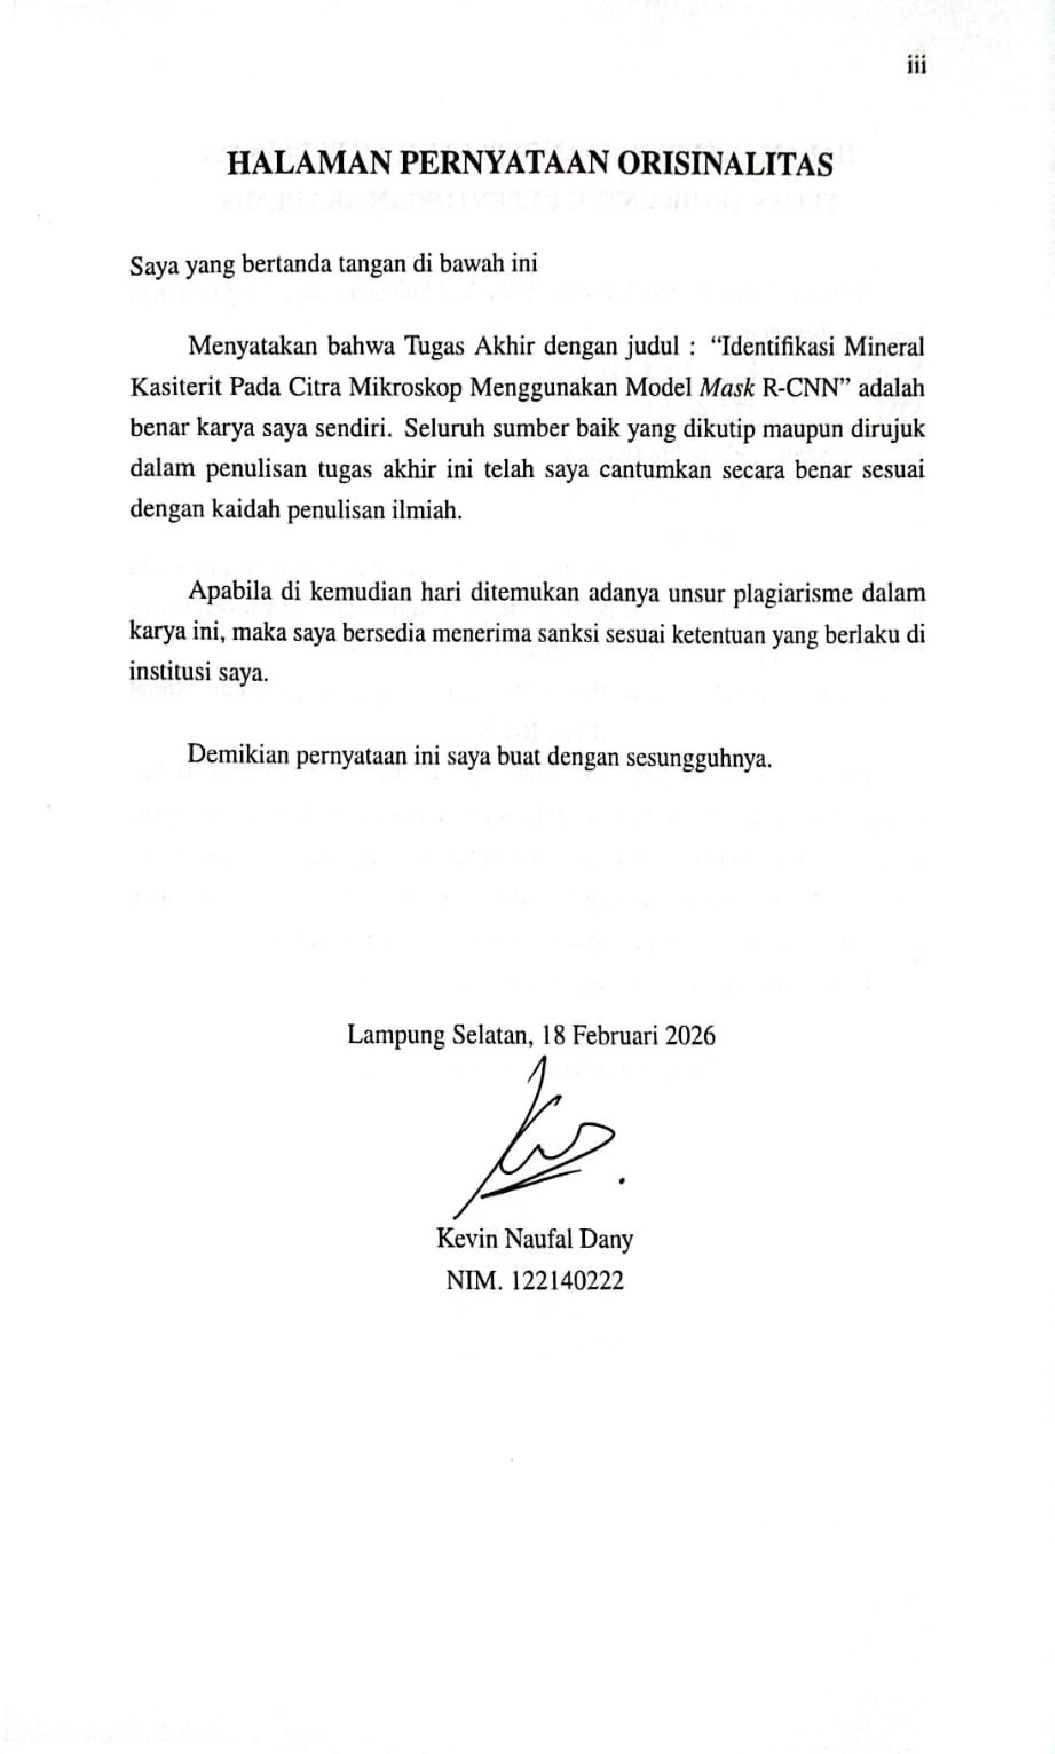
\includepdf[
    pages=1,
    width=\paperwidth,
    height=\paperheight
]{doc/orisinil.pdf}

\clearpage 		% Halaman Pernyataan Orisinalitas
	\input{chapters/publication} 	% Halaman Persetujuan Publikasi
	\clearpage
\phantomsection% 
\addcontentsline{toc}{chapter}{KATA PENGANTAR}
%\thispagestyle{fancy}

\begin{justifying}
	\large \bfseries \centering \MakeUppercase{Kata Pengantar}\linebreak
	
	\normalsize \normalfont \justifying
	% \textit{Pada halaman ini mahasiswa berkesempatan untuk menyatakan terima kasih secara tertulis kepada pembimbing dan pihak lain yang telah memberi bimbingan, nasihat, saran dan kritik, kepada mereka yang telah membantu melakukan penelitian, kepada perorangan atau lembaga yang telah memberi bantuan keuangan, materi dan/atau sarana. Cara menulis kata pengantar beraneka ragam, tetapi hendaknya menggunakan kalimat yang baku. Ucapan terima kasih agar dibuat tidak berlebihan dan dibatasi pada pihak yang terkait secara ilmiah (berhubungan dengan subjek/materi penelitian). } \par
	Puji syukur kehadirat Allah SWT atas segala limpahan rahmat, karunia, serta hidayah-Nya sehingga penulis dapat menyelesaikan penyusunan tugas akhir ini dengan baik. Shalawat serta salam semoga senantiasa tercurah kepada Nabi Muhammad SAW yang telah membawa umat manusia menuju jalan yang penuh ilmu pengetahuan. Penyusunan tugas akhir ini tidak terlepas dari berbagai arahan, bantuan, doa, serta dukungan dari banyak pihak. Oleh karena itu, pada kesempatan ini penulis menyampaikan rasa terima kasih yang sebesar-besarnya kepada: \par
	\begin{enumerate}
		\item Kedua orang tua saya, Bapak Pamuji Waskito Raharjo dan Mamak Anik Purwanti, yang selalu memberikan dukungan, doa yang tiada henti, biaya pendidikan, serta cinta yang tulus sehingga saya dapat menyelesaikan setiap langkah dalam perjalanan perkuliahan ini.
		\item Kedua adik saya, Delfy Celcilia dan Atha Rasyid Risky, yang selalu memberikan semangat, dukungan, dan doa dalam setiap langkah perjalanan saya.
		\item Keluarga besar saya, Nenek Sarmi, Mbah Surati, keluarga besar Bapak, keluarga besar Ibu, serta seluruh kerabat yang selalu memberikan dukungan dan doa yang tulus.
		\item Bapak Martin Clinton Tosima Manullang, Ph.D. dan Ibu Leslie Anggraini, S.Kom., M.Cs. selaku Dosen Pembimbing yang telah meluangkan waktu, memberikan bimbingan, arahan, dukungan moral dan material, serta berbagai masukan yang sangat berharga selama proses penyusunan tugas akhir ini.
		\item Bapak Imam Eko Wicaksono, S.Si., M.Si., Bapak Meida Cahyo Untoro, S.Kom., M.Kom. dan Bapak Andika Setiawan, S.Kom., M.Cs. selaku Dosen Penguji yang telah memberikan saran, kritik, dan masukan yang konstruktif untuk meningkatkan kualitas tugas akhir ini.
		\item Ibu Winda Yulita, M.Cs. dan Ibu Leslie Anggraini, S.Kom., M.Cs. selaku Dosen Wali yang memberikan bimbingan, dukungan, serta perhatian selama masa perkuliahan.
		\item Bapak Hadi, Bapak Ahmad, Bapak Paul, Bapak Mesa, dan Bapak Wiko dari PT Timah Tbk yang telah memberikan ide, saran, waktu, serta menyediakan segala kebutuhan penelitian sehingga penelitian ini dapat terlaksana dengan baik.
		\item Rahma Nur Fadillah, wanita hebat yang telah menemani perjalanan perkuliahan dari awal hingga akhir, memberikan dukungan, semangat, dan doa yang tiada henti. Terima kasih atas segala bantuan dan motivasi yang selalu kamu berikan.
		\item Rekan seperjuangan Coconut Boys, INLINEER 22, Keprofesian HMIF, Grub bimbingan iMUL dan LIA, yang telah memberikan dukungan, semangat, serta berbagai bantuan selama masa perkuliahan. Terima kasih atas kebersamaan dan pertemanan yang luar biasa.
		\item Semua pihak yang tidak dapat saya sebutkan satu per satu yang telah memberikan dukungan, bantuan, serta doa selama perjalanan perkuliahan ini. Terima kasih atas segala kontribusi yang telah diberikan.
	\end{enumerate} \par
	Penulis menyadari bahwa penulisan tugas akhir ini masih jauh dari sempurna dan memiliki banyak kekurangan. Oleh karena itu, penulis sangat terbuka dan mengharapkan saran serta kritik yang bersifat membangun untuk perbaikan di masa mendatang. Akhir kata, penulis berharap semoga tugas akhir ini dapat memberikan manfaat bagi kita semua.
	\vfill
	
\end{justifying}
\clearpage





\begin{comment}
\clearpage
\pagestyle{fancy}
\fancyhf{}
\fancyhead[R]{\thepage}
\phantomsection% 
%\clearpage
%\phantomsection% 
\addcontentsline{toc}{chapter}{KATA PENGANTAR}
%\thispagestyle{fancy}

\begin{justifying}
	\large \bfseries \centering \MakeUppercase{Kata Pengantar}\linebreak
	
	\normalsize \normalfont \justifying
	Puji syukur kehadirat Tuhan Yang Maha Esa atas limpahan rahmat, karunia, serta petunjuk-Nya sehingga penyusunan tugas akhir ini telah terselesaikan dengan baik. Dalam penyusunan tugas akhir ini penulis telah banyak mendapatkan arahan, bantuan, serta dukungan dari berbagai pihak. Oleh karena itu pada kesempatan ini penulis mengucapan terima kasih kepada: \par
	\begin{enumerate}
		\item Bapak Prof. Dr. I. Nyoman Pugeg Aryantha selaku Rektor Institut Teknologi Sumatera.  
		\item Bapak Hadi Teguh Yudistira, S.T., Ph.D. selaku Dekan Fakultas Teknologi Industri.
		\item Bapak Andika Setiawan, S. Kom., M. Cs. selaku Ketua Program Studi Teknik Informatika.
		\item Bapak Ilham Firman Ashari, S. Kom., M.T. selaku Koordinator Tugas Akhir Program Studi Teknik Informatika.  
		\item Bapak Martin C. T. Manullang, Ph.D. selaku Dosen Pembimbing atas ide, waktu, tenaga, perhatian, dan masukan yang telah disumbangsihkan kepada penulis.
            \item Bapak Andika Setiawan, S. Kom., M. Cs dan Bapak Eko Dwi Nugroho, S.Kom., M.Cs. selaku Dosen Penguji atas saran dan masukan yang diberikan. 
		\item Kedua Orang Tua dan Adik yang selalu memberikan dukungan dan doa sehingga penulis dapat menyelesaikan tugas akhir ini. Kelembutan, dukungan, dan cinta yang kalian berikan selalu menjadi sumber inspirasi dan kekuatan.
		\item Teman-teman penulis yang membantu selama masa perkuliahan yang tidak bisa disebutkan satu persatu.
	\end{enumerate} \par
	Akhir kata penulis berharap semoga tugas akhir ini dapat memberikan manfaat bagi kita semua. Penulis menyadari bahwa tugas akhir ini tidak luput dari kekurangan dan kelemahan, dan penulis  terbuka untuk menerima saran, kritik, dan masukan yang membangun.
	\vfill
	
\end{justifying}
\clearpage
\end{comment} 		% Kata Pengantar
    \input{chapters/motto} 			% Motto
	\clearpage
\phantomsection% 
\addcontentsline{toc}{chapter}{RINGKASAN}
\thispagestyle{fancy}

\begin{center}
	\large \bfseries \MakeUppercase{Ringkasan}\\
	\normalsize \normalfont {\thetitle}\\
	\normalsize \normalfont {\theauthor}\\
	\bigskip
	
	\normalsize \normalfont \justifying
	\normalsize \normalfont \justifying
	% P1: Latar Belakang
	Indonesia merupakan salah satu negara dengan kekayaan sumber daya mineral yang melimpah, termasuk timah. Kasiterit (\senyawatin) merupakan mineral utama pembentuk timah yang secara teoritis mengandung 78\% timah, namun kandungan aktualnya hanya sekitar 73–75\% karena jarang ditemukan dalam bentuk murni. Proses identifikasi mineral kasiterit di Laboratorium Eksplorasi PT. Timah Tbk. saat ini masih mengandalkan metode konvensional \textit{Grain Counting Analysis} (GCA) yang dilakukan secara manual di bawah mikroskop binokuler. Metode ini memiliki sejumlah keterbatasan, di antaranya bersifat subjektif, rentan terhadap kelelahan visual (\textit{eye fatigue}), serta menghasilkan variasi hasil identifikasi antaranalis. Selain itu, keberadaan butiran mineral yang saling tumpang tindih (\textit{occluded}) menyebabkan kesulitan dalam membedakan batas antar butir kasiterit sehingga menurunkan akurasi hasil identifikasi. Oleh karena itu, untuk menangani masalah komputasional karena keterbatasan metode konvesional adalah dengan menggunakan pendekatan berbasis teknologi yang mengidentifikasi mineral pada citra mikroskop menggunakan  \textit{deep learning}. \par

	% P2: Tujuan Penelitian
	Penelitian ini bertujuan untuk: (1) menghasilkan model identifikasi berbasis \textit{Mask} R-CNN yang dapat melakukan segmentasi mineral kasiterit pada citra mikroskop serta \textit{robust} terhadap oklusi melalui teknik \textit{amodal instance segmentation}, sehingga model mampu memprediksi bentuk utuh setiap butir kasiterit meskipun sebagian tertutup; dan (2) melakukan pengujian dan analisis untuk mengetahui performa model \textit{Mask} R-CNN menggunakan metrik \textit{Average Precision} (AP) untuk menilai ketepatan klasifikasi area mineral dan \textit{Intersection over Union} (IoU) untuk mengukur akurasi tumpang tindih antara area segmentasi prediksi dengan area sebenarnya dalam mengidentifikasi mineral kasiterit dari citra mikroskop. \par

	% P3: Rumusan Masalah dan Batasan Masalah
	Berdasarkan permasalahan tersebut, penelitian ini merumuskan dua masalah utama, yaitu: (1) bagaimana merancang dan mengembangkan model identifikasi berbasis \textit{Mask} R-CNN yang dapat melakukan segmentasi mineral kasiterit pada citra mikroskop dan mengatasi oklusi antar butir melalui teknik \textit{amodal instance segmentation}, dan (2) bagaimana mengevaluasi performa model \textit{Mask} R-CNN menggunakan metrik AP dan IoU dalam mengidentifikasi mineral kasiterit dari citra mikroskop. Adapun batasan dalam penelitian ini adalah bahwa penelitian hanya berfokus pada identifikasi mineral kasiterit (\senyawatin) dan tidak mencakup identifikasi mineral ikutan lainnya. Dataset yang digunakan sebanyak 142 citra mikroskop trinokuler yang bersumber dari Laboratorium Eksplorasi PT. Timah Tbk. yang berlokasi di Kota Pangkalpinang, Bangka Belitung, dengan proses segmentasi data dilakukan menggunakan perangkat lunak LabelMe yang terintegrasi dengan \textit{Segment Anything}. \par
	
	% Pemilihan \textit{Mask} R-CNN didasarkan pada kemampuannya dalam melakukan deteksi dan \textit{instance segmentation} secara presisi pada citra berlatar belakang kompleks, sementara pendekatan \textit{amodal} memungkinkan model memprediksi bentuk utuh objek meskipun sebagian tertutup. \par

	% P4: Metodologi Penelitian (diperluas)
	Metodologi penelitian diawali dengan tahap identifikasi masalah, di mana ditemukan bahwa proses identifikasi mineral kasiterit di Laboratorium Eksplorasi PT. Timah Tbk. masih dilakukan secara manual menggunakan metode konvensional GCA. Tahap pengumpulan data menghasilkan 142 citra mikroskop mineral kasiterit yang merupakan data sekunder dari Laboratorium Eksplorasi PT. Timah Tbk. Prapemrosesan data meliputi pemilihan data berdasarkan kriteria kualitas pencahayaan dan kejelasan objek, anotasi dan segmentasi data menggunakan metode poligon yang menghasilkan 7.664 objek kasiterit, pembagian citra (\textit{image tiling}) dengan grid $2 \times 2$ yang meningkatkan jumlah objek menjadi 8.433 dengan total 537 \textit{tiles}, augmentasi data menggunakan teknik \textit{flip} horizontal dan vertikal, \textit{rotate} dengan rentang $-15$ hingga $15$ derajat, serta penambahan \textit{Gaussian noise} dengan variansi 0{,}2, dan normalisasi untuk menyeragamkan rentang nilai piksel citra. Pembagian data menggunakan metode \textit{k-fold cross validation} dengan $K=5$ dan rasio 80:20 pada setiap iterasi. Pengembangan model dilakukan dengan melatih dua model \textit{pre-trained} \textit{Mask} R-CNN berbasis \textit{backbone} ResNet50 FPN versi V1 dan V2, dengan dua jenis model \textit{standard} dan \textit{amodal} serta dua variasi \textit{optimizer} SGD dan \textit{Adam}. Evaluasi kinerja model dilakukan menggunakan metrik standar \textit{COCO} yang meliputi AP dan IoU pada beberapa ambang batas, yaitu 0{,}50, 0{,}75, dan 0{,}50:0{,}95, dengan metrik utama \APrangefiftyy dan \IoUrangefiftyy. \par

	% P5: Hasil Evaluasi dan Analisis Optimizer Adam vs SGD
	Hasil evaluasi menunjukkan bahwa model \textit{pre-trained Mask} R-CNN ResNet50 FPN V1 dengan pendekatan \textit{Amodal} dan \textit{optimizer Adam} menghasilkan performa terbaik dengan nilai rata-rata \APrangefiftyy sebesar 0{,}458 dan \IoUrangefiftyy sebesar 0{,}915. Model terbaik kedua adalah \textit{Mask} R-CNN ResNet50 FPN V2 dengan pendekatan \textit{Standard} dan \textit{optimizer} SGD yang memperoleh nilai \APrangefiftyy sebesar 0{,}449 dan \IoUrangefiftyy sebesar 0{,}915, dengan selisih \APrangefiftyy sebesar 0{,}009 terhadap model terbaik pertama. Secara keseluruhan, analisis terhadap seluruh konfigurasi pelatihan menunjukkan bahwa penggunaan \textit{optimizer Adam} secara konsisten menghasilkan performa yang lebih unggul dibandingkan \textit{optimizer} SGD. Keunggulan ini disebabkan oleh mekanisme \textit{adaptive learning rate} yang dimiliki \textit{Adam}, yang mampu mempercepat dan menstabilkan proses konvergensi terutama pada objek dengan bentuk kompleks seperti butir mineral kasiterit pada citra mikroskop. \par
	
	% Pada model V1, penggunaan \textit{Adam} menghasilkan \APrangefiftyy yang lebih tinggi baik pada pendekatan \textit{Amodal} (0{,}458 vs 0{,}446) maupun \textit{Standard} (0{,}450 vs 0{,}437), dengan selisih masing-masing sebesar 0{,}012 dan 0{,}013. Pola serupa juga terlihat pada model V2, di mana \textit{Adam} mengungguli SGD pada pendekatan \textit{Amodal} dengan selisih yang lebih signifikan sebesar 0{,}019 (0{,}420 vs 0{,}401). 
	
	% P6: Penerapan Amodal di Setiap Model Pre-trained
	Penerapan teknik \textit{Amodal Instance Segmentation} menunjukkan pengaruh yang berbeda pada masing-masing model \textit{pre-trained}. Pada model \textit{pre-trained Mask} R-CNN ResNet50 FPN V1 dengan \textit{optimizer Adam}, penambahan teknik \textit{amodal} yang meningkatkan jumlah parameter sebesar 2.950.914 (sekitar 6{,}75\%) terbukti efektif meningkatkan performa, ditunjukkan oleh kenaikan nilai \APrangefiftyy sebesar 0{,}021 (dari 0{,}437 menjadi 0{,}458) serta peningkatan \IoUrangefiftyy sebesar 0{,}005 (dari 0{,}910 menjadi 0{,}915), dengan penambahan waktu pelatihan sebesar 0{,}37 jam yang masih dalam batas komputasi yang dapat diterima. Sebaliknya, pada model \textit{pre-trained Mask} R-CNN ResNet50 FPN V2 dengan \textit{optimizer} SGD, penerapan teknik \textit{amodal} yang meningkatkan jumlah parameter sebesar 2.950.914 (sekitar 6{,}46\%) justru tidak memberikan peningkatan performa. Nilai \APrangefiftyy mengalami penurunan sebesar 0{,}029 (dari 0{,}449 menjadi 0{,}420), sementara \IoUrangefiftyy menurun sebesar 0{,}002 (dari 0{,}915 menjadi 0{,}913), meskipun waktu pelatihan hanya bertambah 0{,}45 jam. Hasil ini menunjukkan bahwa peningkatan kompleksitas model melalui pendekatan \textit{amodal} tidak selalu berbanding lurus dengan peningkatan kinerja, serta mengindikasikan bahwa efektivitas teknik \textit{Amodal Instance Segmentation} sangat bergantung pada kesesuaian arsitektur model \textit{pre-trained} dan pemilihan \textit{optimizer} yang digunakan. \par

	% P7: Hasil Pengujian dan Pengamatan Oklusi
	Pengujian kedua model terbaik dilakukan pada 6 citra uji yang berbeda dari dataset pelatihan. Hasil pengujian menunjukkan perbedaan karakteristik yang jelas antara kedua model. Model V2 \textit{Standard} dengan \textit{optimizer} SGD mampu mengidentifikasi objek kasiterit dengan akurasi deteksi yang tinggi, namun cenderung mengalami \textit{overprediction} yang mengakibatkan tingginya jumlah \textit{False Positive}. Pada data uji ke-5, model V2 \textit{Standard} bahkan menghasilkan nilai \IoUrangefiftyy berupa \textit{NaN}, yang mengindikasikan kegagalan deteksi pada ambang batas IoU tertentu. Sebaliknya, model V1 \textit{Amodal} dengan \textit{optimizer Adam} menunjukkan performa segmentasi yang lebih stabil dan konsisten, ditandai dengan nilai \IoUrangefiftyy yang lebih tinggi secara konsisten serta jumlah \textit{False Positive} yang lebih rendah, meskipun nilai \APrangefiftyy cenderung lebih rendah karena sifat prediksi yang lebih konservatif. Hasil pengamatan visual pada kondisi oklusi memperkuat temuan tersebut, di mana pada kasus kasiterit yang saling bersebelahan dan mengalami oklusi, model V1 \textit{Amodal} mampu memisahkan dan memprediksi masing-masing butir kasiterit secara individual sesuai dengan anotasi \textit{Ground Truth}, sementara model V2 \textit{Standard} cenderung memprediksi area tersebut sebagai satu objek utuh. Lebih lanjut, pada kondisi oklusi oleh elemen latar belakang berupa penanda skala (500 $\mu$m), model V1 \textit{Amodal} masih mampu mendeteksi kasiterit yang tertutup sebagian, sedangkan model V2 \textit{Standard} gagal mendeteksi dan mengabaikan objek tersebut sepenuhnya. \par

	% P8: Kesimpulan
	Berdasarkan hasil penelitian secara keseluruhan, dapat disimpulkan bahwa penelitian ini berhasil merancang dan mengembangkan model identifikasi berbasis \textit{Mask} R-CNN yang dapat melakukan segmentasi mineral kasiterit pada citra mikroskop serta mengatasi oklusi antar butir melalui teknik \textit{amodal instance segmentation}. Model \textit{pre-trained Mask} R-CNN ResNet50 FPN V1 \textit{Amodal} dengan \textit{optimizer Adam} terbukti sebagai konfigurasi terbaik dengan nilai \APrangefiftyy sebesar 0{,}458 dan \IoUrangefiftyy sebesar 0{,}915, didukung evaluasi metrik AP dan IoU melalui skema \textit{k-fold cross validation} yang memberikan gambaran komprehensif terhadap kinerja deteksi dan kualitas segmentasi. Temuan ini menegaskan bahwa pendekatan \textit{amodal instance segmentation} terbukti lebih efektif dan andal untuk identifikasi mineral kasiterit pada citra mikroskop dengan tingkat oklusi yang kompleks dibandingkan pendekatan \textit{standard}. \par

	% P9: Manfaat, Harapan, dan Saran
	Penelitian ini diharapkan dapat memberikan kontribusi sebagai fondasi bagi pengembangan model identifikasi mineral berbasis \textit{deep learning} serta menjadi referensi bagi penelitian selanjutnya yang berkaitan dengan penerapan teknologi \textit{deep learning} dalam bidang geologi dan pertambangan. Untuk pengembangan lebih lanjut, disarankan agar penelitian selanjutnya menerapkan identifikasi pada jenis mineral lain selain kasiterit, mengembangkan model segmentasi yang dapat bekerja secara \textit{real-time} langsung dari mikroskop, menerapkan strategi untuk mengurangi \textit{overprediction}, menerapkan identifikasi jenis kasiterit yang lebih spesifik berdasarkan ciri visual seperti warna, tekstur, atau bentuk kristal, serta menggunakan dua dataset terpisah yakni dataset \textit{amodal} dan \textit{modal} untuk melihat perbedaan hasil penerapan teknik \textit{Amodal Instance Segmentation}. \par


	\vfill
	
\end{center}
\clearpage 		% Ringkasan
	\clearpage
\phantomsection% 
\addcontentsline{toc}{chapter}{ABSTRAK}
\thispagestyle{fancy}

\begin{center}
	\large \bfseries \MakeUppercase{Abstrak}\\
	% \normalsize \normalfont {\thetitle}\\
	% \normalsize \normalfont {\theauthor}\\
	\bigskip
	
	\normalsize \normalfont \justifying \singlespacing
	Identifikasi mineral kasiterit di Laboratorium Eksplorasi PT. Timah Tbk. saat ini masih mengandalkan metode konvensional \textit{Grain Counting Analysis} (GCA) yang dilakukan secara manual menggunakan mikroskop. Metode ini memiliki keterbatasan seperti memerlukan waktu yang lama, bersifat subjektif, dan rentan terhadap kelelahan visual yang menyebabkan tidak konsistennya perhitungan. Penelitian ini bertujuan untuk merancang dan mengembangkan model identifikasi berbasis \textit{Mask} R-CNN yang dapat melakukan segmentasi mineral kasiterit menggunakan dengan teknik \textit{amodal instance segmentation} yang mampu mengatasi permasalahan oklusi antar butir mineral pada citra mikroskop. Pemilihan \textit{Mask} R-CNN didasarkan pada kemampuannya dalam melakukan deteksi dan \textit{instance segmentation} secara presisi pada citra berlatar belakang kompleks, sementara pendekatan \textit{amodal} memungkinkan model memprediksi bentuk utuh objek meskipun sebagian tertutup. Dataset yang digunakan terdiri dari 142 citra mikroskop trinokuler dari Laboratorium Eksplorasi PT. Timah Tbk. yang dianotasi dan divalidasi oleh salah satu tim analis Laboratorium Eksplorasi PT. Timah Tbk. Penelitian ini melatih dua model \textit{pre-trained} \textit{Mask} R-CNN ResNet50 FPN V1 dan V2, dengan dua jenis model \textit{standard} dan \textit{amodal} serta dua variasi \textit{optimizer} SGD dan \textit{Adam}. Evaluasi kinerja model dilakukan menggunakan metrik \textit{Average Precision} (AP) dan \textit{Intersection over Union} (IoU) melalui skema \textit{k-fold cross validation}. Hasil penelitian menunjukkan bahwa model \textit{pre-trained Mask} R-CNN ResNet50 FPN V1 dengan pendekatan \textit{amodal} dan \textit{optimizer Adam} memberikan performa terbaik dengan nilai \APrangefiftyy sebesar 0{,}458 dan \IoUrangefiftyy sebesar 0{,}915, yang menunjukkan kemampuannya dalam melakukan deteksi dan segmentasi kasiterit secara akurat meskipun terjadi oklusi antar butir mineral. Hasil pengujian menunjukkan bahwa model \textit{amodal} Mask R-CNN ResNet50 FPN V1 dengan \textit{optimizer Adam} menghasilkan performa segmentasi yang lebih baik dengan nilai \IoUrangefiftyy yang tinggi dan konsisten, serta hasil prediksi dengan nilai \APrangefiftyy yang stabil, sementara konfigurasi lain masih menunjukkan kecenderungan \textit{overprediction}, terutama pada kondisi oklusi. Penelitian ini menunjukkan bahwa penerapan pendekatan \textit{amodal instance segmentation} terbukti efektif dan andal untuk identifikasi mineral kasiterit pada citra mikroskop dengan tingkat oklusi yang kompleks. \par

    \vspace{20pt}
	\raggedright \textbf{Kata Kunci: Identifikasi Mineral, Kasiterit, \textit{Mask} R-CNN, \textit{Amodal Instance Segmentation}, Citra Mikroskop}
	
	\vfill
	
\end{center}
\clearpage 	% Abstrak (Indonesia)
	\clearpage
\phantomsection% 
\addcontentsline{toc}{chapter}{ABSTRACT}
\thispagestyle{fancy}

\begin{center}
	\large \bfseries \MakeUppercase{Abstract}\\
	% \normalsize \normalfont {\thetitleEN}\\
	% \normalsize \normalfont {\theauthor}\\
	\bigskip
	
	\normalsize \normalfont \justifying \singlespacing
	The identification of cassiterite minerals at the Exploration Laboratory of PT. Timah Tbk. currently still relies on the conventional method of Grain Counting Analysis (GCA), which is performed manually using a microscope. This method has limitations such as being time-consuming, subjective, and prone to visual fatigue, which leads to inconsistent calculations. This study aims to design and develop a \textit{Mask} R-CNN based discovery model that can segment cassiterite minerals using the \textit{amodal instance segmentation} technique that is able to overcome the problem of occlusion between mineral grains in microscope images. The selection of \textit{Mask} R-CNN is based on its ability to perform precise detection and \textit{instance segmentation} on images with complex backgrounds, while the \textit{amodal} approach allows the model to predict the entire shape of an object even if it is partially covered. The dataset used consists of 142 trinocular microscope images from the Exploration Laboratory of PT. Timah Tbk. which were annotated and validated by one of the analyst teams at the Exploration Laboratory of PT. Timah Tbk. This study trained two pre-trained Mask R-CNN ResNet50 FPN V1 and V2 models, with two types of standard and amodal models and two variations of SGD and Adam optimizers. Model performance was evaluated using the Average Precision (AP) and Intersection over Union (IoU) metrics through a k-fold cross validation scheme. The results showed that the pre-trained Mask R-CNN ResNet50 FPN V1 model with the \textit{amodal} approach and \textit{Adam optimizer} provided the best performance with a value of \APrangefiftyy of 0{,}458 and \IoUrangefiftyy of 0{,}915, demonstrating its ability to accurately detect and segment cassiterite despite occlusion between mineral grains. Test results show that the \textit {amodal} Mask R-CNN ResNet50 FPN V1 with \textit{Adam optimizer} produces better segmentation performance with high and consistent \IoUrangefiftyy values, as well as prediction results with stable \APrangefiftyy values, while other configurations still show a tendency toward \textit{overprediction}, especially under occlusion conditions. This study shows that the application of the \textit{amodal instance segmentation} approach is effective and reliable for identifying cassiterite minerals in microscope images with complex occlusion levels. \par


    \vspace{20pt}
	\raggedright\textbf{Keywords: Mineral Identification, Cassiterite, Mask R-CNN, Amodal Instance Segmentation, Microscope Images}
	
	\vfill
	
\end{center}
\clearpage 	% Abstrak (Inggris)    
    %----------------------------------------------------------------%
    % Halaman Daftar
    %----------------------------------------------------------------%    
	% Daftar Isi
	\phantomsection% 
	\addcontentsline{toc}{chapter}{DAFTAR ISI}
	\tableofcontents
	% Daftar tabel
	\phantomsection% 
	\addcontentsline{toc}{chapter}{DAFTAR TABEL}
	\listoftables
	% Daftar gambar
	\phantomsection% 
	\addcontentsline{toc}{chapter}{DAFTAR GAMBAR} % TODO: No halaman ga selang-seling di Daftar? (RDB)
	\listoffigures
	% Daftar rumus
	% \pagestyle{daftarrumusstyle}
	\phantomsection% 
	\addcontentsline{toc}{chapter}{DAFTAR RUMUS}
	\listofmyequations
	% \thispagestyle{daftarrumusstyle}
	% \pagebreak
	%    \input{chapters/symbols}
	% Daftar kode HIDUPIN
	\phantomsection% 
	\addcontentsline{toc}{chapter}{DAFTAR KODE}
	\lstlistoflistings
	\pagebreak
    %----------------------------------------------------------------%
    % Konfigurasi Bab
    %----------------------------------------------------------------%
    \renewcommand{\chaptername}{BAB}
    % Bab: Arabic
    \renewcommand{\thechapter}{\Roman{chapter}}
    % Sub-bab: Roman
    \renewcommand\thesection{\arabic{chapter}.\arabic{section}}
    % Setting supaya nomor halaman pertama dengan "chapter"
    % berada di tengah bawah, tapi selanjut2nya di kanan atas
    \fancypagestyle{plain}{%
    	\fancyhf{}%
    	\renewcommand{\headrulewidth}{0pt}
    	\fancyhead[]{}
    	\fancyfoot[C]{\thepage}
    }
    % Reset penomoran halaman menjadi 1
    \setcounter{page}{1}
    \pagenumbering{arabic}    
    \justifying
    % Mulai selang-seling halaman
    \forceoddpage
    \cleardoublepage
    \pagestyle{alternatingstyle}
    %----------------------------------------------------------------%
    % Daftar Bab
    % Untuk menambahkan daftar bab, buat berkas bab misalnya `chapter-6` di direktori `chapters`, dan masukkan ke sini.
    %----------------------------------------------------------------%
    \newpage

\chapter{PENDAHULUAN} \label{Bab I}

\section{Latar Belakang} \label{I.Latar Belakang}
Indonesia merupakan salah satu negara yang memiliki kekayaan sumber daya mineral yang melimpah, salah satunya adalah timah \cite{PurificationCassiterite4}. Secara historis, Indonesia telah dikenal sebagai produsen timah terbesar di dunia sejak awal abad ke-20 dengan kontribusi yang signifikan terhadap pasar global \cite{IrzonTimahIndonesia12}. Timah (Sn) adalah unsur kimia yang ditemukan dalam bentuk mineral di alam, terutama dalam bentuk kasiterit (\senyawatin) yang merupakan sumber utama timah \cite{IrzonTimahIndonesia12}. Pemanfaatan sumber daya mineral ini memerlukan penerapan metode dan teknologi yang efektif untuk memperoleh hasil yang optimal, menekan biaya produksi, serta memastikan proses yang ramah lingkungan \cite{PurificationCassiterite4}. \par

Kasiterit merupakan mineral utama pembentuk timah yang secara teoritis mengandung 78\% timah, namun karena jarang ditemukan dalam bentuk murni, maka kandungan timahnya hanya sekitar 73–75\% \cite{bookTin} \cite{PurificationCassiterite4}. Wilayah penghasil kasiterit di Indonesia tersebar terutama di Bangka, Belitung, Kundur, Singkep, Karimun, dan Kampar \cite{PurificationCassiterite4}. Pada wilayah-wilayah tersebut, kasiterit umumnya hadir bersama mineral ikutan seperti ilmenit, pasir kuarsa, zirkon, rutil, pirit, kalsit, lantanum, dan monasit, yang menjadi tantangan dalam proses pemisahan untuk memperoleh mineral kasiterit dengan tingkat kemurnian yang tinggi \cite{PurificationCassiterite4} \cite{IrzonTimahIndonesia12}. \par

Salah satu metode identifikasi untuk memperoleh mineral kasiterit adalah metode  \textit{Grain Counting Analysis (GCA)}. GCA merupakan pendekatan konvensional yang digunakan untuk menganalisis jumlah butiran mineral pada sampel guna mengetahui distribusi relatif antara mineral utama dan mineral ikutan \cite{KajianPTTimah6}. Proses ini dilakukan secara manual di bawah mikroskop binokuler, di mana seorang analis menghitung butiran mineral satu per satu berdasarkan pengamatan visual \cite{KajianPTTimah6}. Meskipun metode ini telah lama diterapkan dalam kegiatan eksplorasi mineral, penggunaan mikroskop secara intensif dan berulang berpotensi menimbulkan kelelahan visual (\textit{eye fatigue}), gangguan muskuloskeletal, serta menurunkan konsentrasi kerja, sehingga berdampak pada akurasi dan konsistensi hasil analisis \cite{VisualTrain8} \cite{ConcernAssociated7}. \par

PT. Timah Tbk. merupakan perusahaan pertambangan timah terbesar di Indonesia yang memiliki peran penting dalam kegiatan eksplorasi, penambangan, dan pengolahan bijih timah \cite{PTTimahWebsite}. Saat ini, proses identifikasi dan analisis kuantitatif mineral kasiterit di Laboratorium Eksplorasi PT. Timah Tbk., masih mengandalkan metode GCA. Berdasarkan hasil wawancara pada tanggal 13 Agustus 2025 dengan Bapak Mesa Madestriasa selaku Kepala Laboratorium Eksplorasi PT. Timah Tbk., diketahui bahwa metode ini memiliki sejumlah keterbatasan, terutama berkaitan dengan subjektivitas analis. Satu sampel yang sama dapat dihitung berulang kali dan menghasilkan estimasi yang berbeda, karena sangat bergantung pada ketelitian serta konsistensi analis dalam melakukan pengamatan di bawah mikroskop. Hal ini menimbulkan kekhawatiran akan kemungkinan terjadinya subjektif oleh analis. Adapun salah satu solusi untuk menangani masalah komputasional karena keterbatasan metode konvesional adalah dengan menggunakan pendekatan berbasis teknologi yang mengidentifikasi mineral pada citra mikroskop menggunakan  \textit{deep learning} \cite{ImprovedMaskRCNNOrePanggangan}. \par

Pada beberapa tahun terakhir, \textit{deep learning} berbasis \textit{Convolutional Neural Network} (CNN) terbukti efektif dalam berbagai bidang, khususnya model berbasis \textit{Mask Region-based Convolutional Neural Network} (\textit{Mask} R-CNN) yang mampu melakukan deteksi dan \textit{instance segmentation} secara andal pada citra berlatar belakang kompleks \cite{OreSegmentation2} \cite{ImprovedMaskRCNNOrePanggangan}. Beberapa penelitan sebelumnya telah berhasil menerapkan berbagai model untuk identifikasi objek geologis. Seperti penelitian dari penelitian oleh K. Tang, \textit{et al} pada tahun 2025 mengusulkan perbaikan \textit{Mask} R-CNN untuk segmentasi bijih \textit{polymetallic} untuk meningkatkan ketelitian segmentasi pada citra bijih yang mencapai \textit{Mean Intersection over Union} (MIoU) 92,8\% dan \textit{Mean Average Precision} (mAP) 97,2\% yang lebih tinggi daripada Mask R-CNN standar MIoU 85,88\% dan mAP 92,10\% \cite{OreSegmentation2}. Sementara itu, penelitian yang lebih spesifik oleh M.R. Iyas, N.I. Setiawan, dan I.W. Warmada pada tahun 2020 pada mikroskopi petrografi menerapkan Mask R-CNN untuk identifikasi mineral pembentuk batuan dan menunjukkan bahwa model terbaik adalah Model B (ResNet-101 + pencahayaan) dengan \textit{Average Precision} (AP) 58,0\% sebagai yang terbaik, mengungguli Model A (57,8\%), Model C (45,8\%), dan Model D (43,6\%), serta bahwa pencahayaan mikroskop meningkatkan performa sekitar 12–14,4\%  \cite{maskrcnnKalimantanMic}. \par

Seiring dengan perkembangan tersebut, penelitian ini berfokus pada penerapan model \textit{deep learning}, yaitu \textit{Mask} R-CNN. \textit{Mask} R-CNN merupakan model \textit{instance segmentation} yang tidak hanya mampu mendeteksi dan mengklasifikasikan objek, tetapi juga dapat menghasilkan masker piksel yang presisi untuk setiap butir mineral kasiterit yang terdeteksi \cite{MaskRcnnIEEE11}. \textit{Instance segmentation} merupakan teknik \textit{computer vision} tingkat lanjut yang mengidentifikasi dan mengklasifikasikan setiap objek individu pada tingkat piksel guna memberikan pemahaman komposisi visual yang mendalam dan akurat. Berbeda dengan deteksi objek yang hanya menggunakan kotak pembatas (\textit{bounding box}) untuk lokalisasi, \textit{instance segmentation} mampu menentukan batas setiap objek secara presisi melalui masker piksel, sehingga sangat krusial untuk mencapai lokalisasi yang akurat pada objek-objek berukuran kecil dalam citra yang kompleks \cite{segmentasi-deteksiobjek}. Pendekatan ini sangat sesuai untuk analisis citra mikroskop dalam mendeteksi setiap butir mineral kasiterit, di mana butir-butir mineral sering kali saling tumpang tindih (\textit{occluded}). 

Fenomena tumpang tindih antarobjek (\textit{occlusion}) merupakan kondisi ketika sebagian area objek tertutup oleh objek lain sehingga informasi bentuk yang terlihat pada citra menjadi tidak utuh. Kondisi ini menyulitkan model dalam mempelajari representasi morfologi butir mineral secara konsisten dan berpotensi menurunkan akurasi segmentasi. Meskipun \textit{Mask} R-CNN memiliki kemampuan yang baik dalam melakukan segmentasi objek, citra butir mineral menghadirkan tantangan tersendiri berupa tumpang tindih (\textit{occlusion}) antarbutir yang sering terjadi. Untuk mengatasi permasalahan tersebut, penelitian ini mengusulkan penerapan teknik \textit{amodal instance segmentation}, di mana model dilatih untuk mengidentifikasi bentuk utuh dari setiap butir mineral kasiterit meskipun sebagian areanya tertutup oleh butir lainnya \cite{FoodMaskRCNN10}.

Untuk mengukur performa model yang diusulkan, evaluasi dilakukan menggunakan metrik standar \textit{COCO} yang meliputi \textit{Average Precision} (AP) dan \textit{Intersection over Union} (IoU) \cite{MaskRcnnIEEE11}. \textit{Intersection over Union} (IoU) digunakan untuk mengukur tingkat ketepatan tumpang tindih antara area segmentasi hasil prediksi dengan area segmentasi sebenarnya. Sementara itu, \textit{Average Precision} (AP) merupakan rata-rata presisi yang dihitung pada berbagai ambang batas IoU dan menilai keseimbangan antara tingkat presisi dan \textit{recall} model. Hasil evaluasi ini digunakan sebagai acuan dalam penilaian kinerja model, analisis performa segmentasi, serta sebagai dasar perbaikan dan pengembangan penelitian serupa di masa mendatang \cite{OreSegmentation2}. \par

\section{Rumusan Masalah} \label{I.Rumusan Masalah}
Berdasarkan latar belakang yang telah diuraikan, dapat diidentifikasi beberapa rumusan masalah pada penelitian ini, di antaranya :

\begin{enumerate}[noitemsep]
	\item Bagaimana merancang dan mengembangkan model identifikasi berbasis \textit{Mask} R-CNN yang dapat melakukan segmentasi mineral kasiterit pada citra mikroskop dan mengatasi oklusi antar butir melalui teknik \textit{amodal instance segmentation}?
	\item Bagaimana mengevaluasi performa model \textit{Mask} R-CNN menggunakan metrik AP dan IoU dalam mengidentifikasi mineral kasiterit dari citra mikroskop?
\end{enumerate}

\section{Tujuan Penelitian} \label{I.Tujuan}
Berdasarkan rumusan masalah yang telah diuraikan, penelitian ini memiliki tujuan sebagai berikut:

\begin{enumerate}[noitemsep]
	\item Menghasilkan model identifikasi berbasis \textit{Mask} R-CNN yang dapat melakukan segmentasi mineral  kasiterit pada citra mikroskop serta robust terhadap oklusi melalui teknik \textit{amodal instance segmentation}.
	\item Melakukan pengujian dan analisis untuk mengetahui hasil performa model \textit{Mask} R-CNN menggunakan metrik AP untuk menilai tingkat ketepatan klasifikasi area mineral dan IoU untuk mengukur akurasi tumpang tindih antara area segmentasi hasil prediksi dengan area sebenarnya dalam mengidentifikasi mineral kasiterit dari citra mikroskop.
\end{enumerate}

\section{Batasan Masalah} \label{I.Batasan}
Batasan masalah dalam penelitan ini dibuat untuk  menghindari penelitian keluar dari fokus dan memastikan pencapaian tujuan yang realistis. Adapun batasan-batasan dalam penelitian ini adalah sebagai berikut:

\begin{enumerate}[noitemsep]
	\item Penelitian ini hanya berfokus pada identifikasi mineral kasiterit (\senyawatin) dan tidak mencakup identifikasi mineral ikutan lainnya seperti ilmenit, kuarsa, zirkon, rutil, atau monasit.
	\item Dataset yang digunakan sebanyak 142 citra mikroskop trinokuler yang bersumber  dari Laboratorium Eksplorasi PT. Timah Tbk yang berlokasi di Kota Pangkalpinang, Bangka Belitung.
	\item Citra butir mineral kasiterit yang digunakan ber-ekstensi *.jpg.
	% mencakup 7664 butir mineral kasiterit.
	% sebanyak 1053 citra mikroskop dan 
	\item Proses anotasi data dilakukan menggunakan perangkat lunak LabelMe with SAM dan tidak mengeksplorasi tools anotasi lainnya \cite{Wada_Labelme_Image_Polygonal}.
\end{enumerate}

\section{Manfaat Penelitian} \label{I.Manfaat}
Penelitian ini diharapkan dapat memberikan manfaat bagi berbagai pihak, antara lain:

\begin{enumerate}[noitemsep]
	\item Mengetahui mineral kasiterit secara otomatis dari citra mikroskop menggunakan teknologi \textit{deep learning}.
	\item Meningkatkan efisiensi dalam proses identifikasi mineral kasiterit di laboratorium.
	\item Memberikan fondasi untuk pengembangan model identifikasi mineral lainnya seperti ilmenit, kuarsa, zirkon, rutil, dan monasit dalam penelitian selanjutnya.
	\item Menjadi referensi bagi penelitian selanjutnya yang berkaitan dengan penerapan teknologi \textit{deep learning} dalam bidang geologi dan pertambangan.
\end{enumerate}

\section{Sistematika Penulisan} \label{I.Sistematika}
Sistematika penulisan berisi pembahasan apa yang akan ditulis disetiap Bab. Sistematika pada umumnya berupa paragraf yang setiap paragraf mencerminkan bahasan setiap Bab. \par

\subsection{Bab I Pendahuluan}
Bab ini berisi pengantar penelitian yang menjabarkan latar belakang, rumusan masalah, tujuan penelitian, batasan masalah, manfaat penelitian, serta sistematika penulisan. \par

\subsection{Bab II Tinjauan Pustaka}
Bab ini membahas mengenai tinjauan pustaka dari penelitan terdahulu dan dasar teori yang berkaitan dengan penelitian ini.

\subsection{Bab III Metodologi Penelitian}
Bab ini berisikan penjelasan alur kerja sistem, alat dan data yang digunakan, metode yang digunakan, dan rancangan pengujian.

\subsection{Bab IV Hasil dan Pembahasan}
Bab ini membahas hasil implementasi dan pengujian dari penelitian yang dilakukan, serta analisis dan evaluasi yang dapat dipetik dari hasil.

\subsection{Bab V Kesimpulan dan Saran}
Bab ini membahas kesimpulan dari hasil penelitian dan juga saran untuk penelitian selanjutnya.
    \newpage
\chapter{TINJAUAN PUSTAKA} \label{Bab II}

\section{Tinjauan Pustaka} \label{II.Tinjauan}
Tinjauan pustaka berisi berbagai penelitian terdahulu yang memiliki kesamaan topik dengan penelitian ini dan digunakan sebagai referensi utama. Penelitian ini merujuk pada beberapa studi literatur yang membahas metode serta pendekatan yang akan diterapkan. Berikut adalah beberapa penelitian yang di jadikan acuan.\par

Penelitian yang dilakukan oleh N. Aditama dan R. Munir pada tahun 2022 mengusulkan metode estimasi kalori makanan jalanan Indonesia menggunakan \textit{Mask} R-CNN untuk segmentasi makanan dan \textit{Multiple Linear Regression} (MLR) untuk estimasi kalori yang menerapkan teknik \textit{amodal instance segmentation} menggunakan beberapa \textit{backbone} seperti ResNet-101-FPN dan ResNetXt-101-FPN. Dataset terdiri dari 1.646 citra makanan dengan enam kelas mencakup 4.530 total objek menggunakan optimizer \textit{Stochastic Gradient Descent} (SGD). Hasil pengujian terbaik diperoleh menggunakan \textit{Mask} R-CNN ResNeXt-101-FPN dengan nilai \textit{F1-Score} sebesar 0,821 pada kondisi tertutup dengan \textit{F1-Score} sebesar 0,994 pada kondisi tidak tertutup, dan rata-rata R² = 0,80425 pada model regresi \cite{FoodMaskRCNN10}. \par

Penelitian yang dilakukan oleh K. Tang, \textit{et.al} pada tahun 2025 yang mengembangkan \textit{Improved Mask} R-CNN dengan menambahkan  \textit{Re-parameterized Refocus Convolution} (RefConv) dan \textit{Efficient Channel Attention} (ECA). Dataset yang digunakan berjumlah 3,500 gambar yang dilatih selama 100 epoch. Hasil eksperimen berhasil meningkatkan ketelitian segmentasi pada citra bijih yang mencapai MIoU 92,8\% dan mAP 97,2\% yang lebih tinggi daripada Mask R-CNN standar MIoU 85,88\% dan mAP 92,10\% menunjukkan bahwa kombinasi RefConv dan ECA berhasil meningkatkan kemampuan model dalam meningkatkan akurasi segmentasi \cite{OreSegmentation2}. \par

Penelitian yang dilakukan oleh H. Zhou, G. Cai, dan S. Liu pada tahun 2023 mengusulkan \textit{Improved Mask} R-CNN untuk mendeteksi bijih yang bertumpuk menggunakan arsitektur ResNet-101 dengan modifikasi \textit{Multipath Feature Pyramid Network} (MFPN) yang memperkaya detail fitur dari citra bijih. Dataset yang digunakan berjumlah 1,000 gambar yang dilatih selama 200 epoch menggunakan \textit{optimizer Adam}. Hasil eksperimen menunjukkan peningkatan kinerja dengan nilai $AP_{75}$ dengan jaringan fusi fitur yang ditingkatkan mencapai sekitar 73,12\%, sekitar 6,64\% lebih tinggi dibanding \textit{Mask} R-CNN standar \cite{ImprovedMaskRCNNOrePanggangan}. \par

Penelitian yang dilakukan oleh B.A.P. Ferreira, \textit{et.al} pada tahun 2024 mengusulkan penerapan \textit{Mask} R-CNN untuk mengidentifikasi dan melakukan segmentasi partikel kuarsa pada citra mikroskop bijih besi menggunakan pendekatan \textit{instance segmentation}. Dataset terdiri dari 865 citra yang berisi 1.740 partikel kuarsa yang dilabel secara manual menggunakan perangkat VGG \textit{Image Annotator} (VIA) dengan menggunakan \textit{backbone} ResNet-101 dengan optimasi menggunakan \textit{stochastic gradient descent}. Hasil pengujian menunjukkan performa yang sangat baik dengan \textit{precision} sebesar 95,22\%, \textit{recall} 88,46\%, dan \textit{F1-score} 91,72\% yang menunjukkan kemampuan tinggi model dalam mengenali dan memisahkan partikel kuarsa dari latar belakang kompleks \cite{QuartzMicMaskrcnn}. \par

Penelitian yang dilakukan oleh M.R. Iyas, N.I. Setiawan, dan I.W. Warmada pada tahun 2020 mengusulkan penggunaan \textit{Mask} R-CNN untuk identifikasi mineral pembentuk batuan pada citra \textit{petrography} menggunakan empat model berbeda berdasarkan pencahayaan mikroskop \textit{Plane Polarized Light} (PPL) dan \textit{Cross Polarized Light} (XPL) serta jenis \textit{backbone} (ResNet-50 dan ResNet-101). Hasil pengujian menunjukkan bahwa model terbaik adalah Model B (ResNet-101 + pencahayaan) dengan AP 58,0\% sebagai yang terbaik, mengungguli Model A (57,8\%), Model C (45,8\%), dan Model D (43,6\%), serta bahwa pencahayaan mikroskop meningkatkan performa sekitar 12–14,4\% \cite{maskrcnnKalimantanMic}. \par
 
Penelitian yang dilakukan oleh E.J.Y. Koh, \textit{et.al} pada tahun 2021 melakukan penelitian mengenai otomatisasi analisis mineralogi menggunakan dua algoritma segmentasi berbasis \textit{deep learning}, yaitu \textit{Mask} R-CNN dan SOLO v2. Dataset terdiri atas 122 citra mikroskop dengan tiga kelas utama. Model Mask R-CNN dilatih selama 303 epoch dengan hasil $AP_{coco}$ sebesar 44,3\% dengan 5 frame/detik, sementara SOLO v2 di latih selama 45 epoch menghasilkan $AP_{coco}$ sebesar 50,4\% dengan 20 frame/detik yang menunjukan bahwa model \textit{instance segmentation} mampu mendeteksi mineral secara cepat dan akurat \cite{mineralogiMaskRCNNSolo}. Berikut pada Tabel \ref{table:2.Tinjauan} dilampirkan ringkasan tinjauan pustaka terdahulu. \par

% Penelitian yang dilakukan oleh L. Qi, \textit{et.al} mengusulkan metode \textit{amodal instance segmentation} melalui pengenalan dataset baru, KINS (KITTI INStance dataset). Mereka mengusulkan arsitektur \textit{Amodal Segmentation Network} (ASN) untuk memprediksi bentuk utuh objek termasuk bagian yang tidak terlihat atau teroklusi, yang menerapkan teknik \textit{Multi-Level Coding} (MLC) dan sebuah \textit{Occlusion Classification Branch}. Metode ini diimplementasikan di atas \textit{baseline} \textit{state-of-the-art} seperti \textit{Mask} R-CNN. Dataset KINS terdiri dari 14.991 total citra, dibagi menjadi 7.474 citra latih dan 7.518 citra uji, dengan anotasi padat untuk 7 kategori objek. Model dilatih menggunakan optimizer \textit{Stochastic Gradient Descent} (SGD). Hasil pengujian menunjukkan ASN meningkatkan kinerja \textit{baseline} secara signifikan, di mana \textit{Mask} R-CNN + ASN menghasilkan rata-rata presisi (\textit{mAP}) sebesar 32{,}7\% untuk deteksi (dibanding 31{,}3\%), 31{,}1\% untuk \textit{amodal segmentation} (dibanding 29{,}3\%), dan 28{,}7\% untuk \textit{inmodal segmentation} (dibanding 26{,}6\%) \cite{AmodalASN}. Berikut pada Tabel \ref{table:2.Tinjauan} dilampirkan ringkasan tinjauan pustaka terdahulu.\par

% Atur margin untuk landscape - bisa disesuaikan nilai left dan right
\newgeometry{top=2cm, bottom=1.75cm, left=2.25cm, right=2cm}
\begin{landscape}
% \thispagestyle{landscape} % Untuk page number yang benar di landscape
\begin{longtable}{|p{0.2cm}|p{1.6cm}|p{2.4cm}|p{2.5cm}|p{2.5cm}|p{2.5cm}|p{3.5cm}|}
	\caption{Penelitian Terdahulu}
	\label{table:2.Tinjauan}\\
	\hline
	\multicolumn{1}{|c|}{\textbf{No.}} & 
	\multicolumn{1}{c|}{\textbf{Peneliti}} & 
	\multicolumn{1}{c|}{\textbf{Judul}} & 
	\multicolumn{1}{c|}{\textbf{Metode Seleksi Fitur}} & 
	\multicolumn{1}{c|}{\textbf{Permasalahan}} & 
	\multicolumn{1}{c|}{\textbf{Metode Klasifikasi}} &
	\multicolumn{1}{c|}{\textbf{Hasil}} \\
	\hline
	\endfirsthead
	
	% \multicolumn{7}{c}{\tablename\ \thetable\ -- \textit{Lanjutan dari halaman sebelumnya}} \\
	\hline
	\multicolumn{1}{|c|}{\textbf{No.}} & 
	\multicolumn{1}{c|}{\textbf{Peneliti}} & 
	\multicolumn{1}{c|}{\textbf{Judul}} & 
	\multicolumn{1}{c|}{\textbf{Metode Seleksi Fitur}} & 
	\multicolumn{1}{c|}{\textbf{Permasalahan}} & 
	\multicolumn{1}{c|}{\textbf{Metode Klasifikasi}} &
	\multicolumn{1}{c|}{\textbf{Hasil}} \\
	\hline
	\endhead
	
	\hline
	% \multicolumn{7}{r}{\textit{Bersambung ke halaman berikutnya}} \\
	\endfoot
	
	\hline
	\endlastfoot
	
	1. & 
	N. Aditama, dan R. Munir (2022) \cite{FoodMaskRCNN10}& 
	\textit{Indonesian Street Food Calorie Estimation using Mask R-CNN and Multiple Linear Regression} & 
	ResNet-101-FPN, ResNeXt-101-FPN, \textit{Amodal instance segmentation} & 
	Segmentasi pada citra makanan dengan objek yang saling menutupi \textit{(occlusion)} serta variasi bentuk yang kompleks & 
	\textit{Mask} R-CNN, \textit{Multiple Linear Regression} & 
	Model ResNeXt-101-FPN mencapai \textit{F1-score} 0,821 pada kondisi tertutup, 0,994 pada kondisi tidak tertutup, dan R² 0,80425 untuk regresi kalori \\
	\hline
	
	2. & 
	K. Tang, \textit{et al.} (2025) \cite{OreSegmentation2}& 
	\textit{Improvement of Mask R-CNN Algorithm for Ore Segmentation} & 
	\textit{Re-parameterized Refocus Convolution} (RefConv), \textit{Efficient Channel Attention} (ECA), ResNet-50  & 
	Segmentasi bijih \textit{polymetallic nodules} kurang akurat pada model standar akibat hilangnya detail tepi & 
	\textit{Improvement Mask} R-CNN & 
	Model \textit{Improvement Mask} R-CNN menghasilkan MIoU 92,8\% dan mAP 97,2\% yang meningkat signifikan dari model standar dengan MIoU 85,88\% dan mAP 92,10\% \\
	\hline
	 
	3. & 
	H. Zhou, G. Cai, dan S. Liu (2023) \cite{ImprovedMaskRCNNOrePanggangan}& 
	\textit{Research on stacked ore detection based on improved Mask RCNN under complex background} & 
	\textit{Multipath Feature Pyramid Network} (MFPN) dengan ResNet-101 & 
	Deteksi bijih yang saling bertumpuk pada latar belakang kompleks & 
	\textit{Improvement Mask} R-CNN & 
	Model dengan MFPN mencapai $AP_{75}$ sebesar 73,12\%, meningkat 6,64\% dibanding \textit{Mask} R-CNN standar \\
	\hline

	4. & 
	B.A.P. Ferreira \textit{et al.} (2024) \cite{QuartzMicMaskrcnn} & 
	\textit{Instance Segmentation of Quartz in Iron Ore Optical Microscopy Images by Deep Learning} & 
	ResNet-101, VGG \textit{Image Annotator} (VIA) & 
	Segmentasi partikel kuarsa yang memiliki sifat transparan dan warna serupa dengan resin pengikat & 
	\textit{Mask} R-CNN & 
	Model \textit{Mask} R-CNN mencapai \textit{precision} sebesar 95,22\%, \textit{recall} 88,46\%, dan \textit{F1-score} 91,72\% dalam segmentasi partikel kuarsa \\
	\hline

	5. & 
	M.R. Iyas, N.I. Setiawan, dan I.W. Warmada (2020) \cite{maskrcnnKalimantanMic}& 
	\textit{Mask R-CNN for rock-forming minerals identification on petrography, case study at Monterado, West Kalimantan} & 
	ResNet-50, ResNet-101, \textit{Plane Polarized Light} (PPL), \textit{Cross Polarized Light} (XPL) & 
	Identifikasi mineral pembentuk batuan pada citra yang dipengaruhi oleh perbedaan pencahayaan mikroskop & 
	\textit{Mask} R-CNN & 
	Model terbaik adalah model B (ResNet-101 dengan pencahayaan) memperoleh AP 58,0\% yang lebih tinggi 12-14\% dibanding model tanpa pencahayaan \\
	\hline

	6. & 
	E.J.Y. Koh \textit{et al.} (2021) \cite{mineralogiMaskRCNNSolo}& 
	\textit{Utilising convolutional neural networks to perform fast automated modal mineralogy analysis for thin-section optical microscopy} & 
	ResNet, SOLO v2, \textit{Feature Pyramid Network} (FPN) & 
	Segmentasi mineral untuk analisis mineralogi modal otomatis pada mikroskop optik \textit{thin-section} & 
	\textit{Mask} R-CNN, SOLO v2 & 
	\textit{Mask} R-CNN menghasilkan $AP_{coco}$ 44,3\% dengan kecepatan 5 frame/ detik, sedangkan SOLO v2 mencapai $AP_{coco}$ 50,4\% dengan kecepatan 20 frame/detik. \\
	\hline

	
	% 7. & 
	% L. Qi \textit{et al.}  & 
	% \textit{Amodal Instance Segmentation with KINS Dataset} (2019) \cite{AmodalASN} & 
	% \textit{Amodal Segmentation Network} (ASN), \textit{Multi-Level Coding} (MLC), Occlusion \textit{Classification Branch} & 
	% Model standar gagal memprediksi bagian objek yang teroklusi \textit{(amodal)} karena \textit{overfitting} pada fitur lokal yang terlihat. & 
	% Mask R-CNN, PANet & 
	% Metode ASN (dengan MLC) meningkatkan mAP sebesar 32{,}7\% untuk deteksi (dibanding 31{,}3\%), 31{,}1\% untuk \textit{amodal segmentation} (dibanding 29{,}3\%), dan 28{,}7\% untuk \textit{inmodal segmentation} (dibanding 26{,}6\%). \\ 
	% \hline
	
\end{longtable}
\end{landscape}
\restoregeometry
% \pagestyle{fancy} % Kembalikan ke pagestyle normal setelah landscape

Berdasarkan informasi yang telah disajikan pada Tabel 2.1, terdapat sejumlah perbedaan dan pembaruan dibandingkan dengan penelitian terdahulu. Penelitian ini berfokus pada identifikasi mineral kasiterit dari citra mikroskop menggunakan model \textit{Mask} R-CNN dengan penerapan teknik \textit{amodal instance segmentation} untuk mengatasi oklusi antarbutir mineral. Evaluasi performa dilakukan menggunakan metrik AP dan IoU guna menilai ketepatan deteksi dan akurasi segmentasi \par

\section{Dasar Teori} \label{II.Teori}
Dasar teori merupakan landasan intelektual yang memberikan pemahaman menyeluruh terhadap konsep-konsep yang relevan dengan penelitian, menjelaskan prinsip-prinsip teoretis yang mendasari kajian, serta membentuk kerangka konseptual yang menjadi acuan dalam pengembangan metode, analisis, dan interpretasi hasil penelitian secara ilmiah dan terarah. \par

\subsection{Kasiterit} \label{II.TeoriKasiterit}
Kasiterit (\senyawatin) dikenal juga dengan nama \textit{Tinstone} merupakan mineral utama pembentuk timah yang secara teoritis mengandung 78\% timah, namun karena jarang ditemukan dalam bentuk murni, maka kandungan timahnya hanya sekitar 73–75\% \cite{PurificationCassiterite4} \cite{bookTin}. Mineral ini memiliki struktur kristal tetragonal yang memiliki sifat \textit{opaque} yang dapat tembus pada sayatan tipis dan kilap \textit{adamantin} hingga \textit{submetallic}. Kasiterit memiliki densitas tinggi (sekitar $7,15~g/cm^3$) yang sangat tahan terhadap pelapukan dan di klasifikasikan sebagai mineral berat \cite{GeochemicalGeologicalTin}. Mineral kasiterit yang di ambil pada citra mikroskop dapat di lihat pada Gambar \ref{fig:2.Kasiterit} berikut. \par

\begin{figure}[H] % Kalau menggunakan H, posisi gambar akan tepat dibawah teks
    \centering
    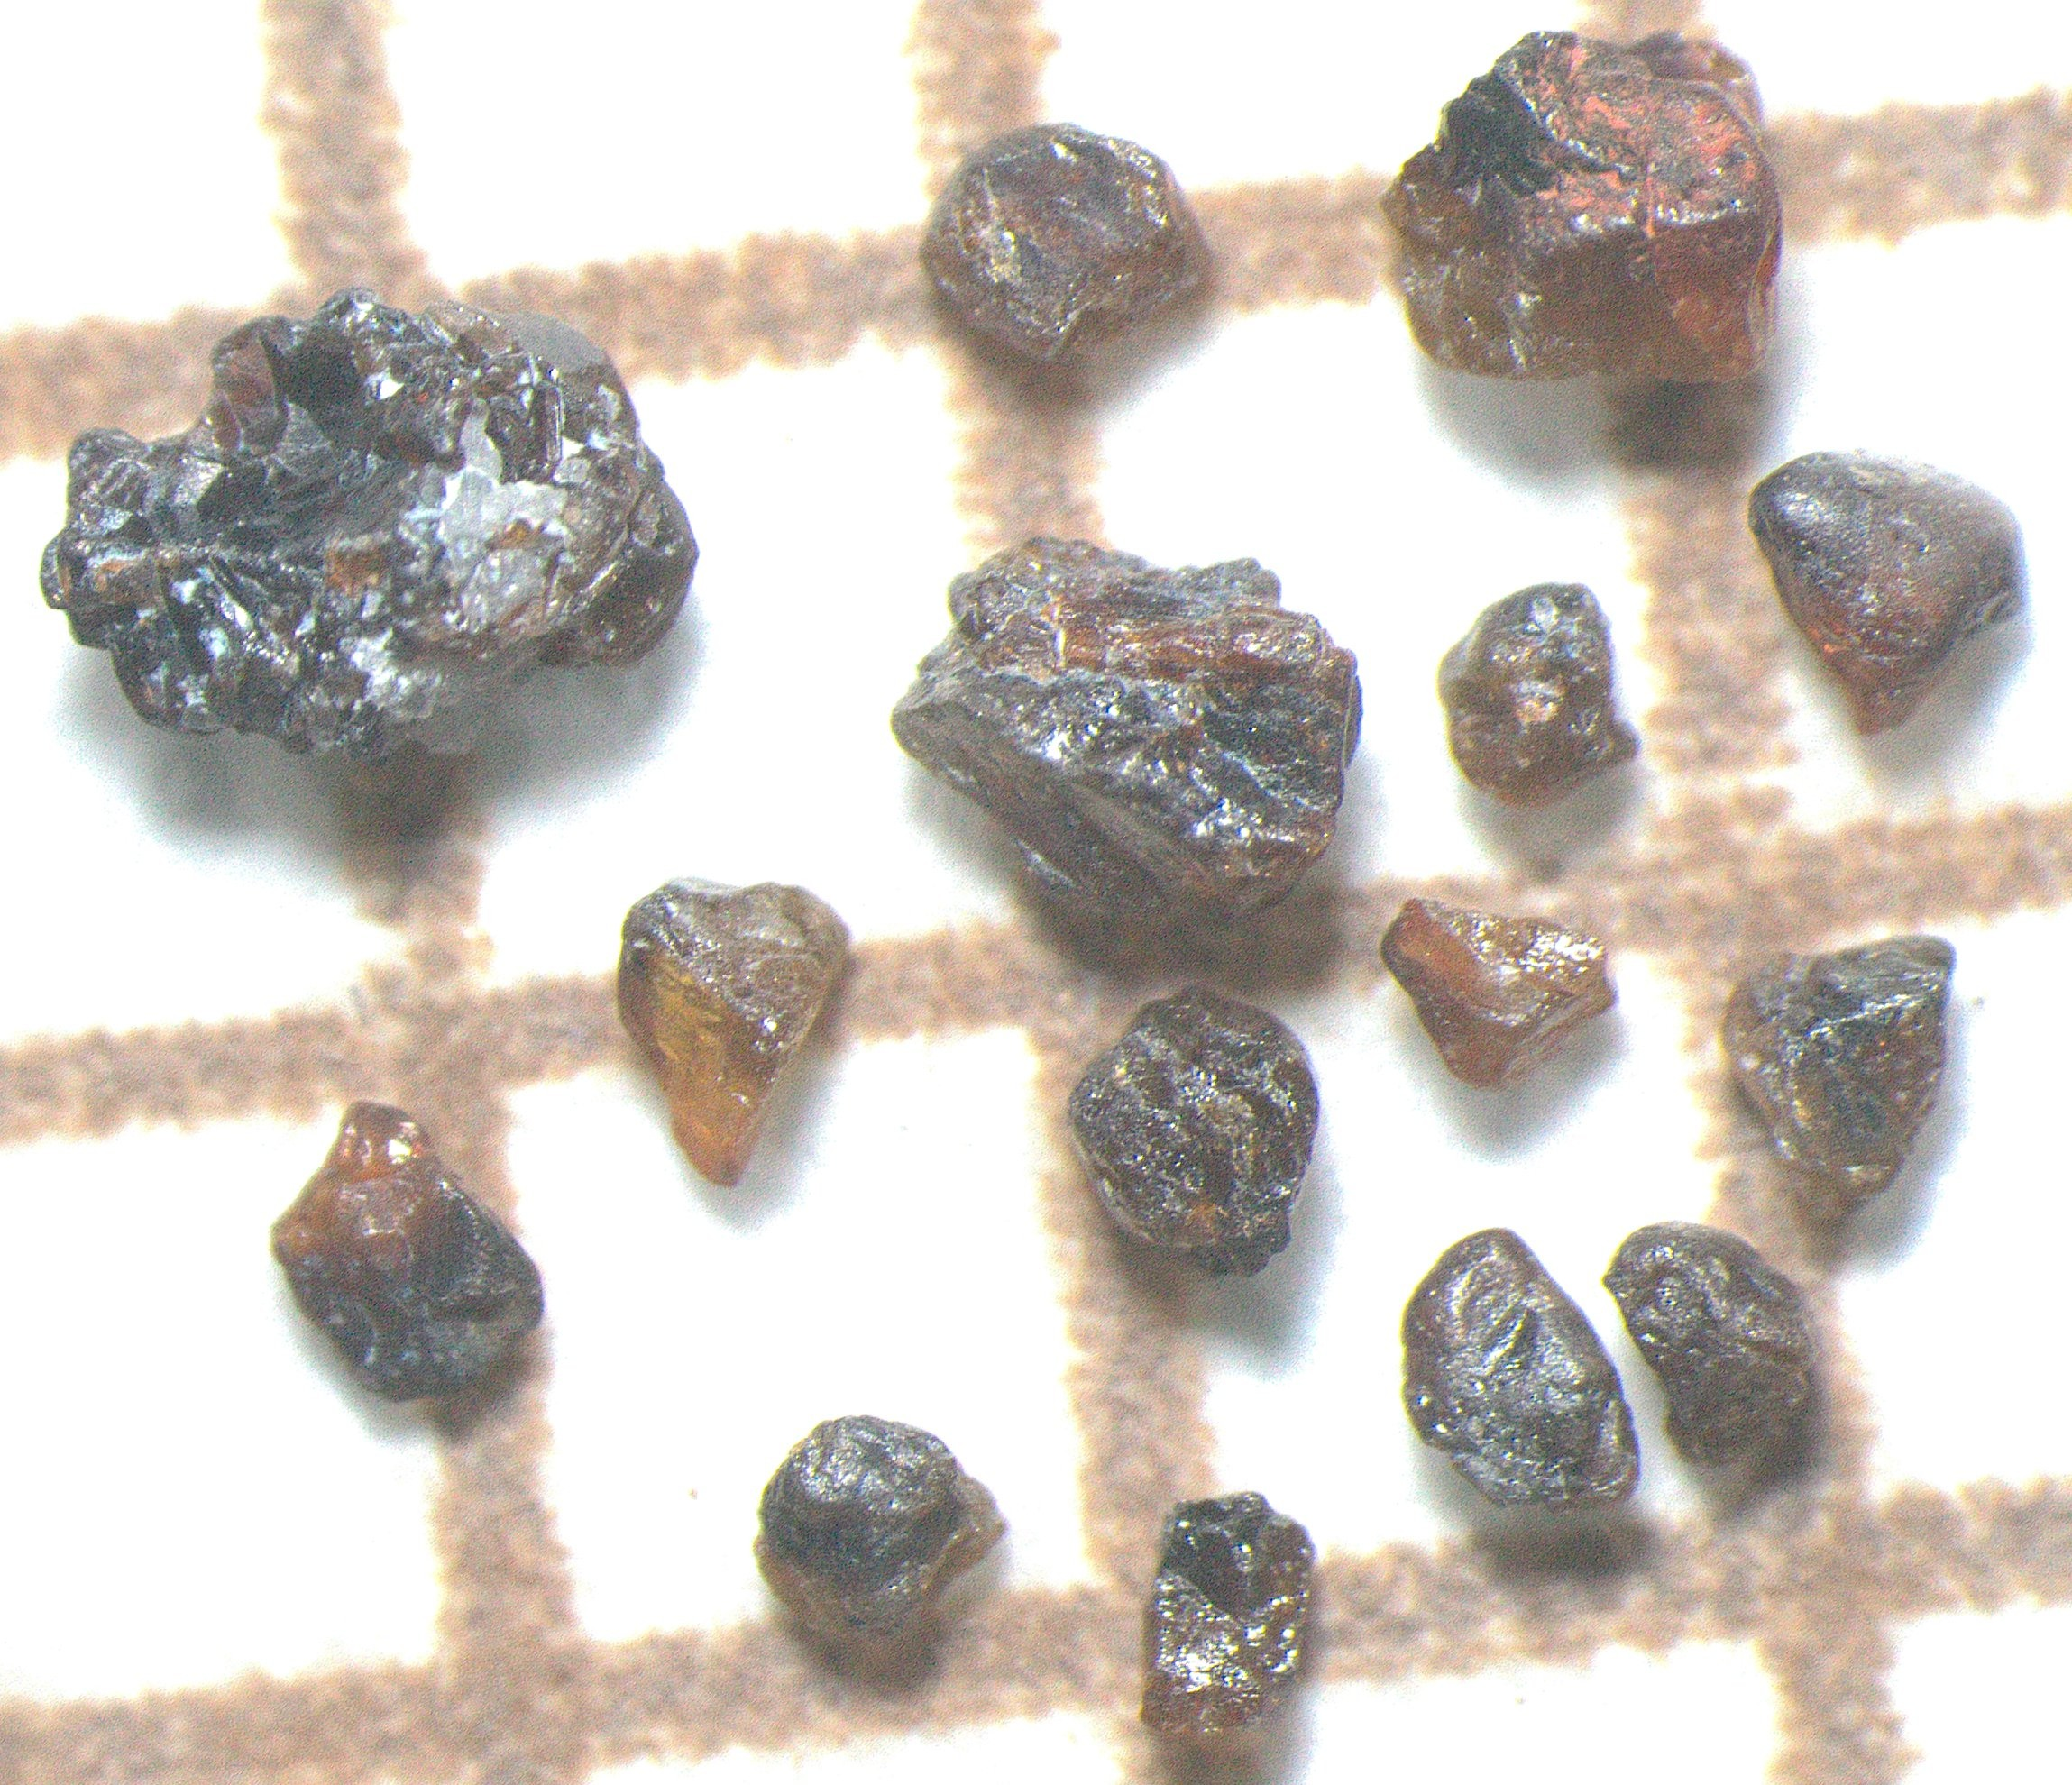
\includegraphics[width=0.5\textwidth]{figure/cassiteriteImg.jpg}
    \caption{Mineral Kasiterit}
    \label{fig:2.Kasiterit}
\end{figure}

Mineral kasiterit umumnya berwarna coklat gelap hingga hitam, meskipun variasi kemerahan atau kekuningan dapat terjadi karena pengotor utama seperti tantalum, niobium, titanium, dan unsur-unsur lainnya dalam bentuk \textit{solid solution} \cite{IrzonTimahIndonesia12} \cite{bookTin}. Setidaknya terdapat 14 mineral pembawa timah lainnya dan sebagian di antaranya hanya ditemukan pada wilayah tertentu \cite{IrzonTimahIndonesia12}. Pada wilayah-wilayah tersebut, kasiterit umumnya hadir bersama mineral ikutan seperti ilmenit, pasir kuarsa, zirkon, rutil, pirit, kalsit, lantanum, dan monasit, yang merupakan sumber potensial unsur tanah jarang (UTJ) \cite{PurificationCassiterite4} \cite{IrzonTimahIndonesia12}. Detail karakteristik kasiterit dapat dilihat pada Tabel \ref{table:ciri2-kasiterit} berikut. \par

\begin{longtable}{|p{0.04\textwidth}|p{0.26\textwidth}|p{0.60\textwidth}|}
\caption{Ciri-ciri Kasiterit}
\label{table:ciri2-kasiterit} \\
\hline
\centering\textbf{No.} & \centering\textbf{Ciri} & \centering\arraybackslash\textbf{Spesifikasi} \\
\hline
\endfirsthead

\hline
\centering\textbf{No.} & \centering\textbf{Ciri} & \centering\arraybackslash\textbf{Spesifikasi} \\
\hline
\endhead

1 &
Warna &
Kasiterit memiliki variasi warna seperti hitam, coklat, coklat gelap, hingga merah gelap, tergantung kondisi mineral dan kandungan unsur jejaknya. \\
\hline

2 &
Kilap &
Kasiterit memiliki kilap minyak (\textit{oil luster}) yang tampak seperti permukaan berminyak saat diamati di bawah mikroskop. \\
\hline

3 &
Bentuk Butir &
Bentuk butir kasiterit umumnya membulat hingga setengah membulat (\textit{rounded} sampai \textit{sub-rounded}) dan tidak bersudut tajam. \\
\hline

4 &
Tekstur Visual &
Pada pengamatan mikroskop, kasiterit sering terlihat memiliki tekstur menyerupai daging atau serat halus. \\
\hline

5 &
Pembeda Utama &
Ciri utama pembeda kasiterit dengan mineral lain yang mirip adalah kilap minyaknya yang khas dibandingkan mineral seperti ilmenit. \\
\hline

6 &
Transparansi &
Kasiterit bersifat opak hingga tembus cahaya (translusen), terutama pada sayatan tipis atau kristal berukuran kecil. \\
\hline

7 &
Goresan (\textit{Streak}) &
Warna goresan kasiterit umumnya coklat pucat hingga putih, dan pada beberapa sampel tidak meninggalkan jejak goresan yang jelas. \\
\hline

\end{longtable}

\subsubsection{Timah} \label{II.TeoriTimah}
Timah (Sn) adalah unsur logam yang di temukan dalam bentuk mineral di alam dengan nomor atom 50 dan massa atom 118,71 \cite{IrzonTimahIndonesia12} \cite{GeochemicalGeologicalTin}. Logam ini memiliki titik lebur yang relatif rendah (232°C) dan ketahanan yang baik terhadap korosi dan oksidasi, membuatnya mudah di dilelehkan dan dilebur yang telah dimanfaatkan manusia sejak ribuan tahun lalu \cite{IrzonTimahIndonesia12}. PT. Timah Tbk. merupakan perusahaan pertambangan timah terbesar di Indonesia yang memiliki peran penting dalam kegiatan eksplorasi, penambangan, dan pengolahan bijih timah \cite{PTTimahWebsite}. Salah satu produk timah yang dihasilkan oleh PT. Timah Tbk dikenal dengan merek dagang Banka, yang merupakan bentuk timah batangan hasil proses peleburan dan pemurnian bijih timah,sebagaimana dapat dilihat pada Gambar \ref{fig:2.TimahBanka} berikut. \par

\begin{figure}[H] % Kalau menggunakan H, posisi gambar akan tepat dibawah teks
	\centering
		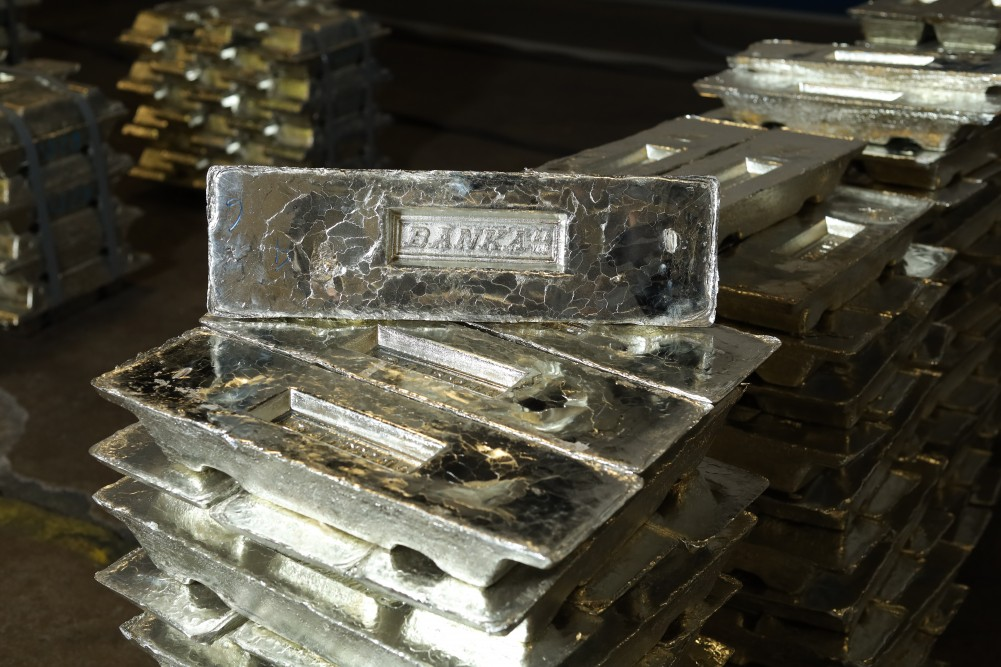
\includegraphics[width=0.5\textwidth]{figure/timahBanka.jpg}
		\caption{Produk Timah (\textit{Brand} Banka) \cite{PTTimahWebsite}}
		\label{fig:2.TimahBanka}
\end{figure}


\subsection{Citra Digital} \label{II.TeoriCitra}
Citra adalah suatu cahaya pada bidang dua dimensi. Secara matematis, citra merupakan fungsi kontinu dari intensitas cahaya pada bidang dua dimensi. Dalam konteks digital, citra adalah kumpulan titik yang dinamakan piksel (\textit{pixel} atau \textit{picture element}) \cite{bookCitra}. Setiap piksel digambarkan sebagai satu kotak kecil yang memiliki koordinat posisi. Sebuah citra digital dapat direpresentasikan sebagai ruang diskrit berdimensi-dua yang berasal dari citra analog melalui proses sampling atau digitalisasi \cite{bookCitra}. \par

\subsubsection{Citra Mikroskop} \label{II.TeoriCitraMikroskop}
Citra mikroskop pada dasarnya adalah kumpulan data intensitas foton yang berfungsi untuk memperlihatkan detail halus dalam struktur suatu objek atau sampel. Citra ini terbentuk ketika cahaya berinteraksi dengan materi yang menyusun sampel yang sedang diamati. Intensitas interaksi cahaya ini, yang menentukan kecerahan gambar, diatur secara tepat menggunakan pengatur intensitas lampu (\textit{rheostat}) \cite{microscope}. Variasi pencahayaan mikroskop berpengaruh terhadap kualitas citra yang dihasilkan, baik dari segi ketajaman maupun kontras objek mineral. Perbandingan tingkat kecerahan tersebut dapat dilihat pada Gambar \ref{fig:2.MicComparison}, yang menunjukkan perbedaan antara citra terlalu gelap, pencahayaan optimal, dan terlalu terang. \par

\begin{figure}[H]
    \centering
    % Baris pertama: dua gambar sejajar
    \begin{subfigure}[b]{0.475\textwidth}
        \centering
        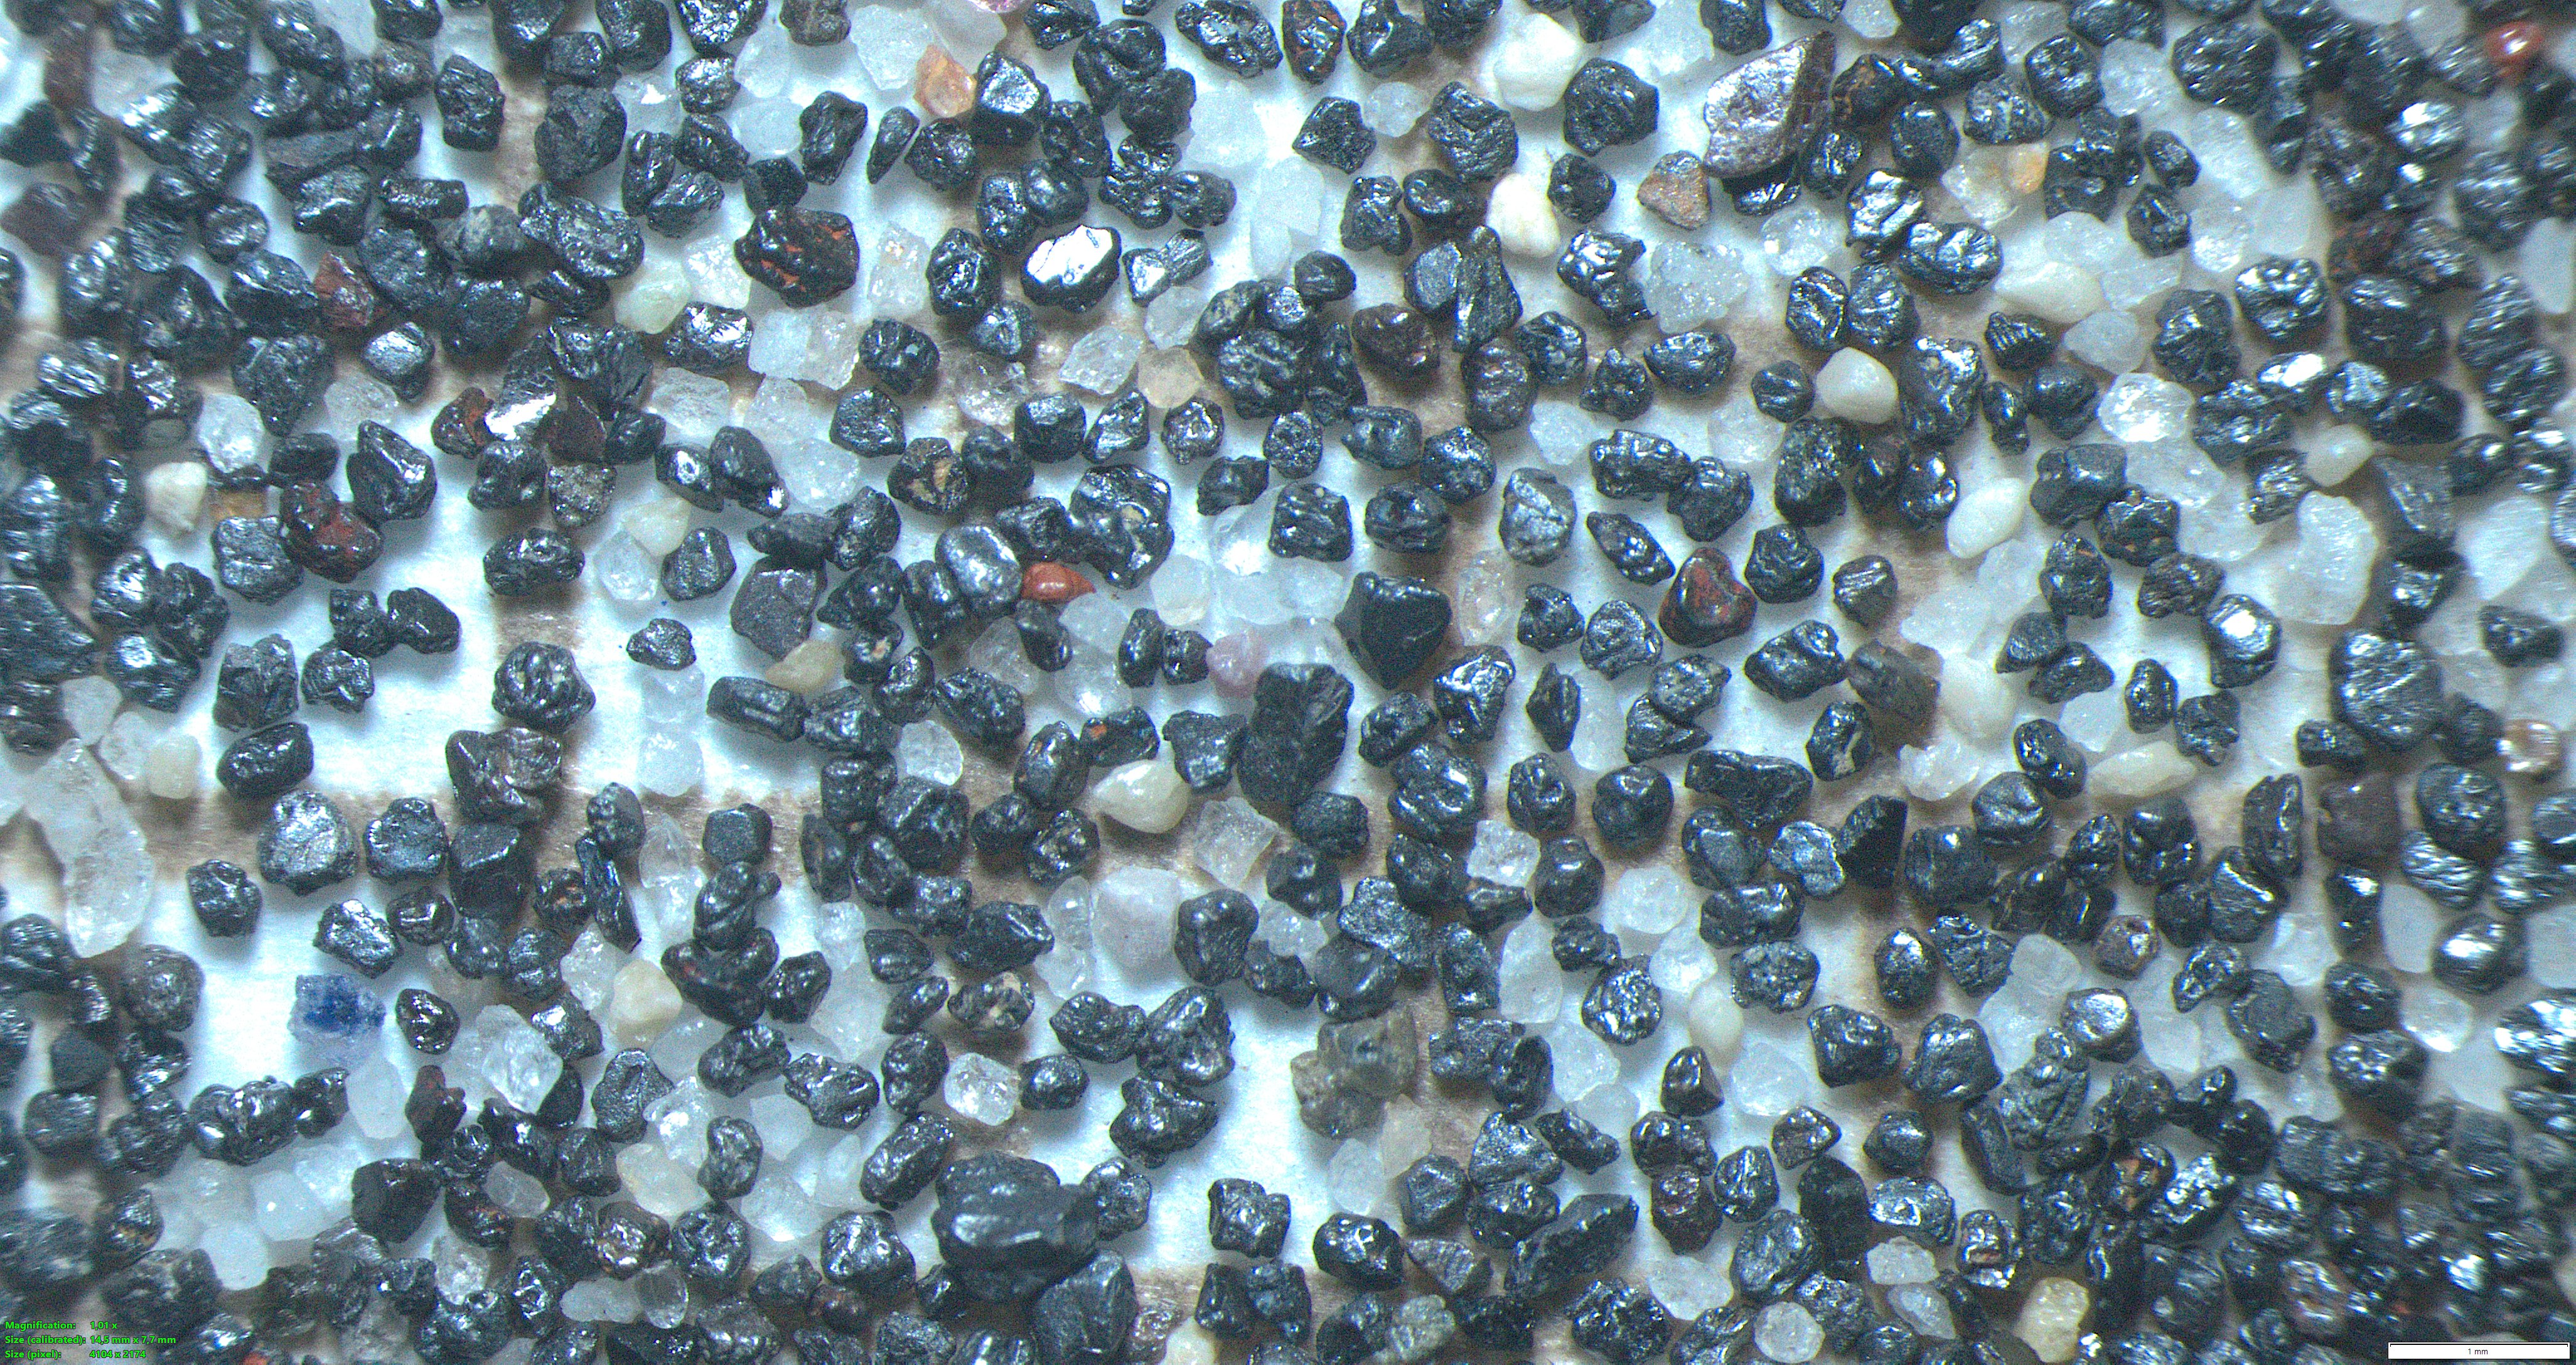
\includegraphics[width=\textwidth]{figure/micGelap.jpg}
        \caption{Kecerahan Citra Mikroskop Terlalu Gelap}
        \label{fig:2.Mic1}
    \end{subfigure}
    \hfill
    \begin{subfigure}[b]{0.475\textwidth}
        \centering
        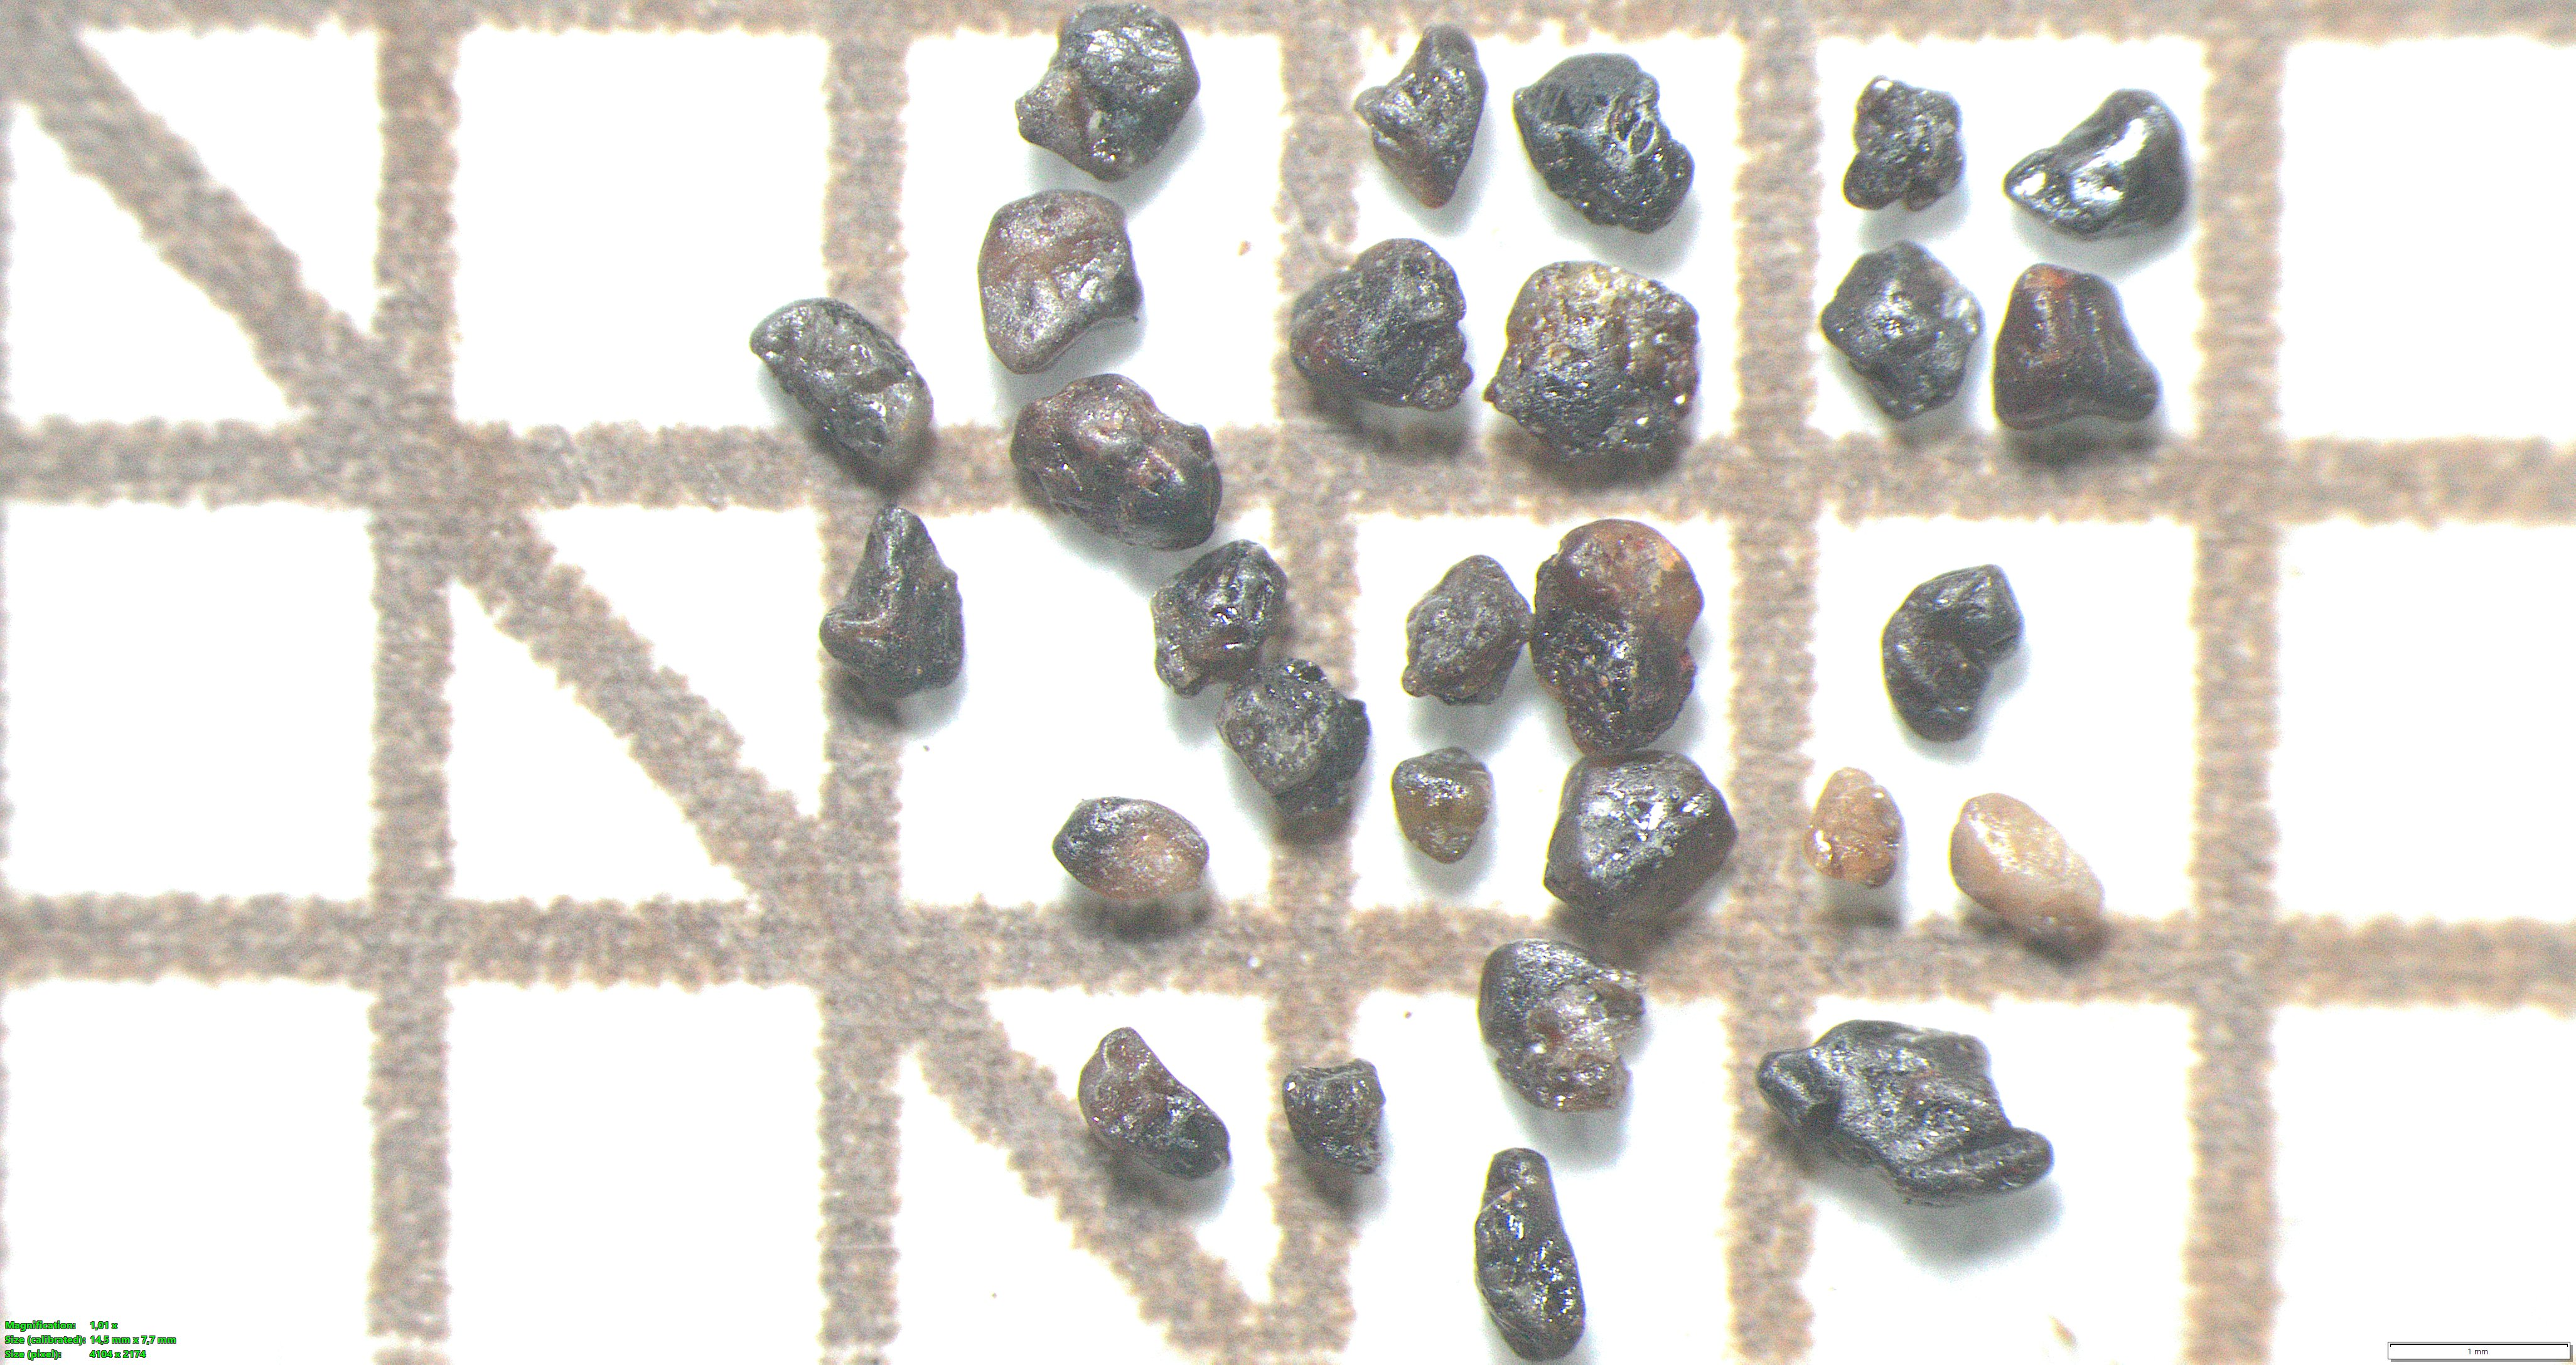
\includegraphics[width=\textwidth]{figure/micTerang.jpg}
        \caption{Kecerahan Citra Mikroskop Terlalu Terang}
        \label{fig:2.Mic3}
    \end{subfigure}
    
    % Baris kedua: satu gambar di bawah tengah
    \vskip\baselineskip
    \begin{subfigure}[b]{0.475\textwidth}
        \centering
        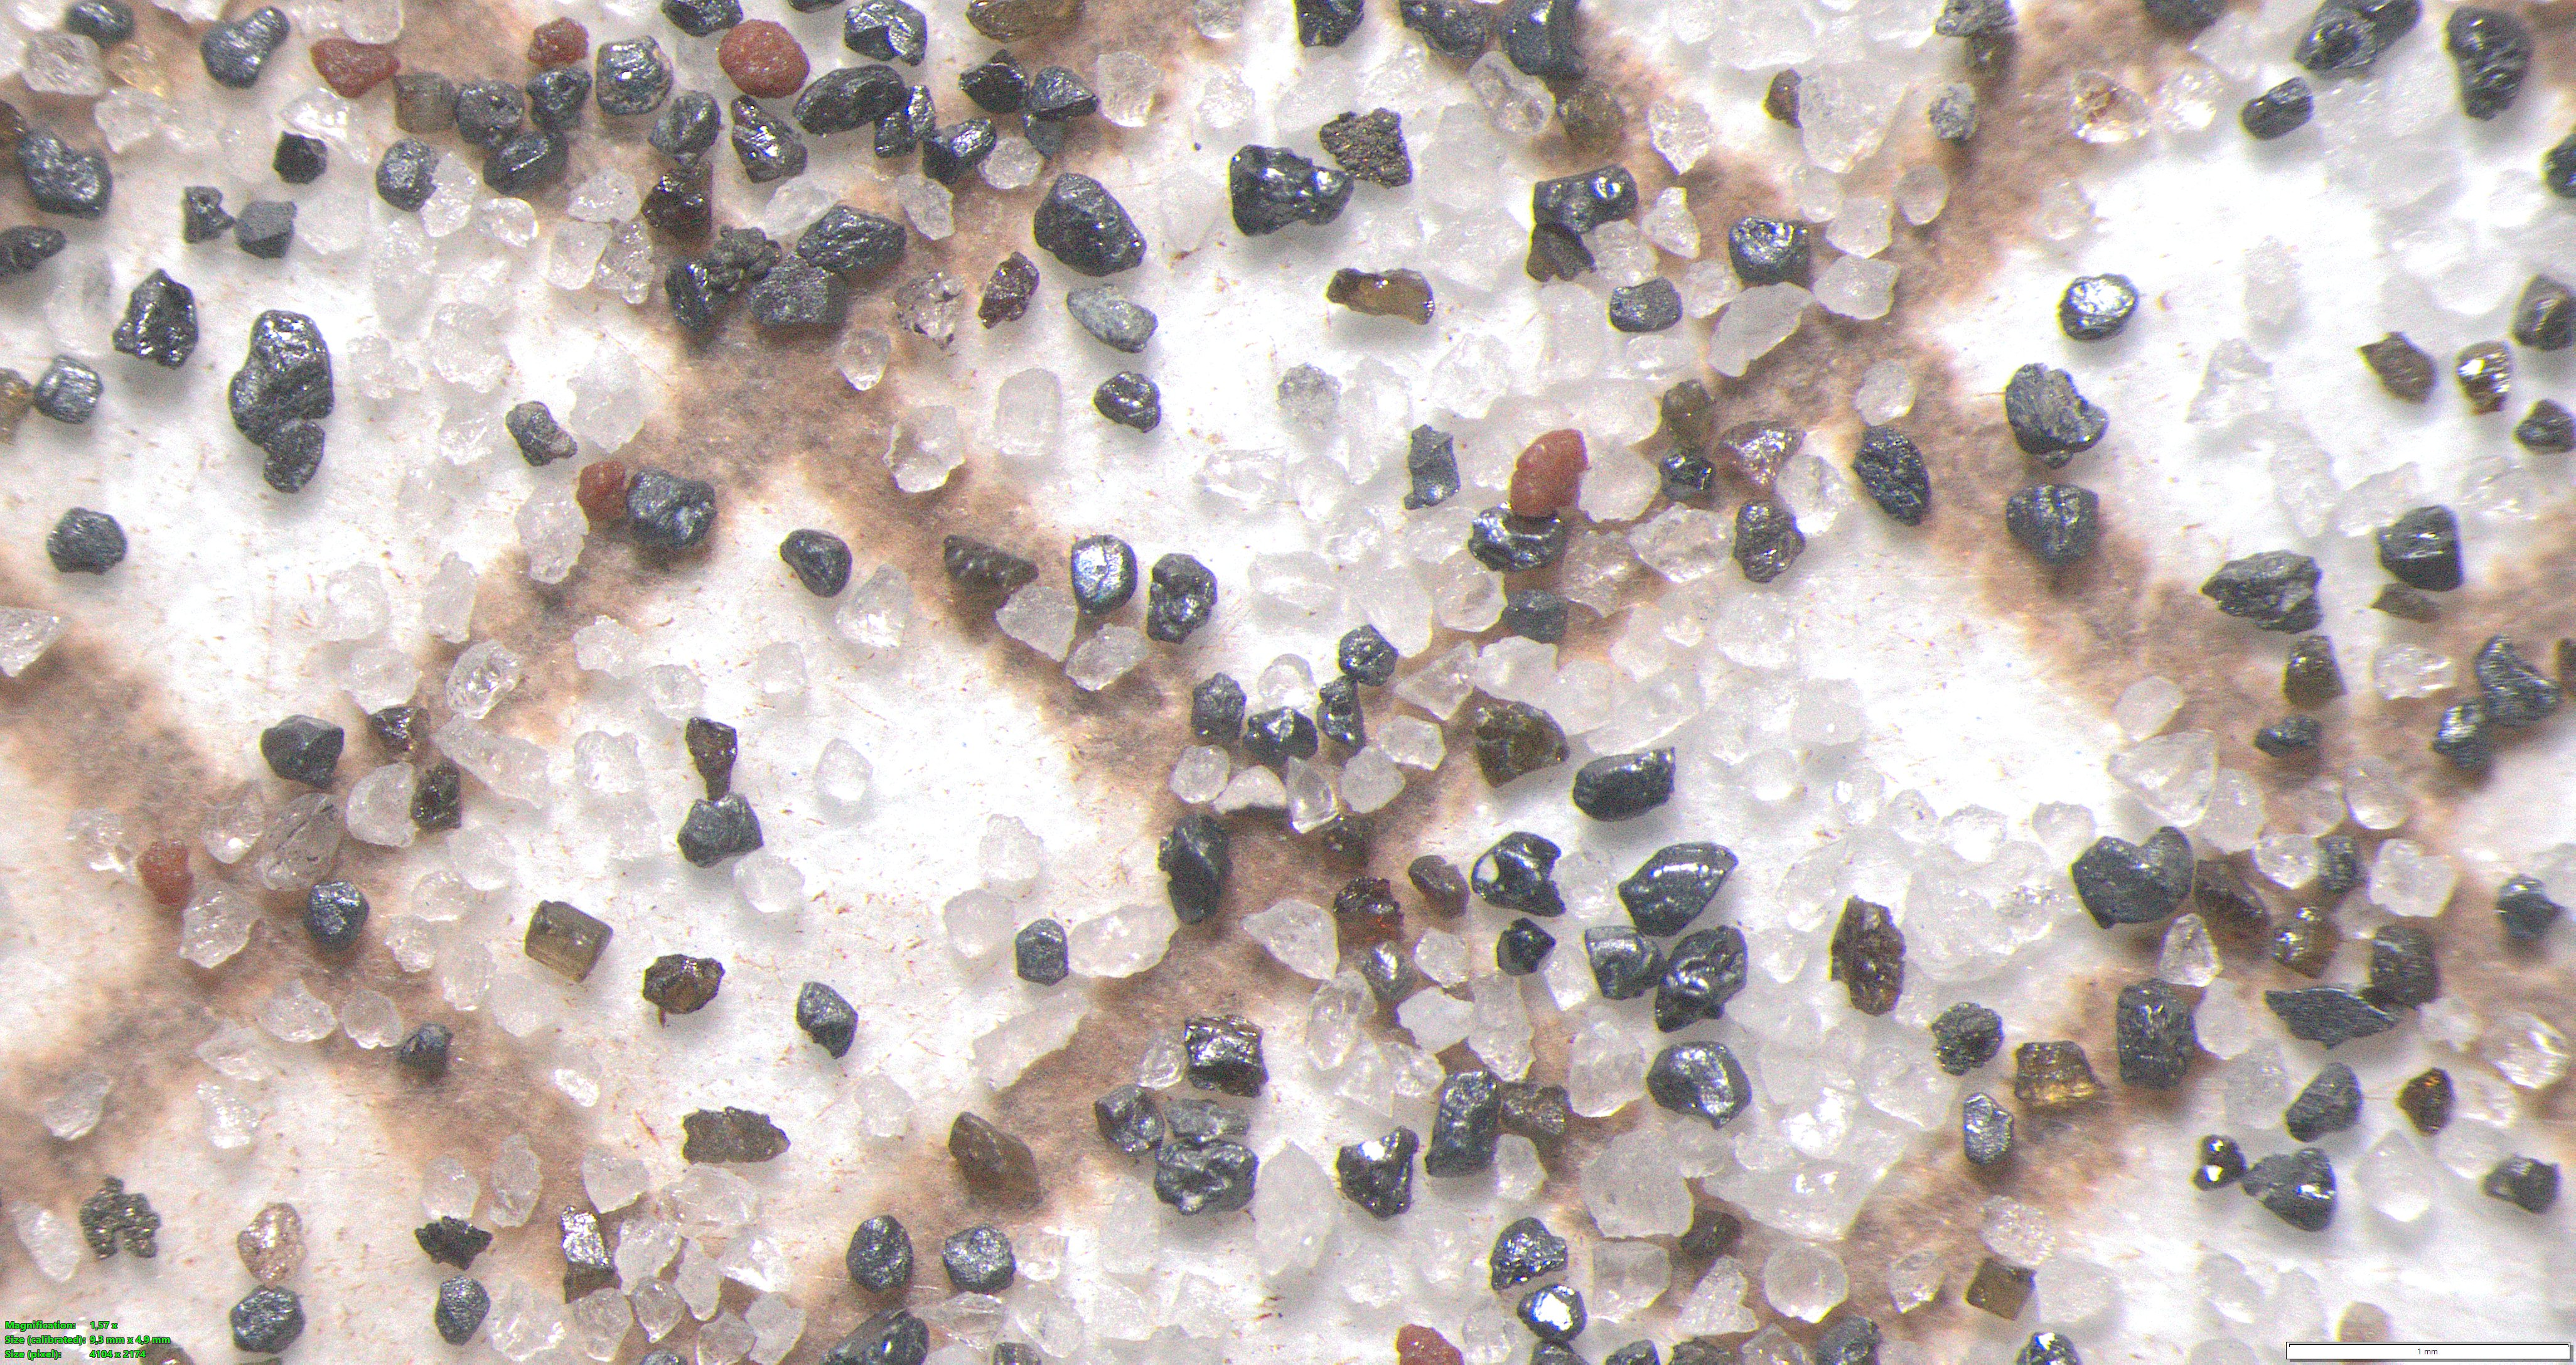
\includegraphics[width=\textwidth]{figure/micSedang.jpg}
        \caption{Kecerahan Citra Mikroskop Optimal}
        \label{fig:2.Mic2}
    \end{subfigure}
    
    \caption{Perbandingan Tingkat Kecerahan Citra Mikroskop}
    \label{fig:2.MicComparison}
\end{figure}

\subsubsection{Ruang Warna RGB} \label{II.Ruang-Warna-RGB}
Citra berwarna, yang sering dikenal dengan istilah truecolor, menggunakan ruang warna RGB untuk menyajikan data visual melalui penggabungan tiga komponen dasar yaitu Merah (Red), Hijau (Green), dan Biru (Blue). Model ini diadopsi secara luas pada perangkat seperti monitor dan kamera video karena reseptor mata manusia dapat merasakan kombinasi ketiga warna ini secara efektif untuk membentuk persepsi visual. Secara teknis, setiap komponen warna dalam sistem ini menggunakan kedalaman 8 bit yang menentukan intensitasnya dalam rentang nilai 0 hingga 255. Dengan variasi intensitas tersebut, ruang warna RGB memungkinkan representasi spektrum yang sangat luas hingga mencapai total 16.581.375 kemungkinan warna yang dapat disajikan \cite{bookCitra}. \par

\subsection{Prapemrosesan Data} \label{II.TeoriPrapemrosesan}
Prapemrosesan data (\textit{data preprocessing}) merupakan tahap awal dalam pengolahan data yang bertujuan untuk meningkatkan kualitas data sebelum data tersebut digunakan ke dalam model. Tahap ini dilaksanakan karena dalam banyak kasus data mentah yang akan digunakan, termasuk pada data yang seringkali mengalami masalah seperti ukuran (dimensi) yang tidak konsisten, orientasi atau posisi objek yang berbeda-beda, skala nilai yang tidak seragam, maupun format atau pencahayaan yang variatif. Dengan melakukan prapemrosesan, data menjadi lebih konsisten, mudah diolah, dan model yang dibangun memiliki peluang konvergensi yang lebih baik serta mampu menghasilkan generalisasi yang lebih baik. \par

\subsubsection{Segmentasi Citra} \label{II.TeoriSegmentasiCitra}
Segmentasi citra adalah proses fundamental dalam pemprosesan citra digital dan visi komputer yang bertujuan mempartisi atau membagi citra menjadi beberapa segmen atau subkelompok piksel, yang sering disebut sebagai \textit{region} atau objek \cite{imageSegmentation} \cite{bookCitra}. Secara teknis, segmentasi melibatkan pemberian label unik pada setiap piksel dalam citra sedemikian rupa sehingga piksel-piksel dengan label yang sama berbagi karakteristik visual tertentu (seperti warna, intensitas, atau tekstur) dan secara kolektif membentuk suatu \textit{region} yang koheren \cite{bookCitra}. 
Segmentasi citra terbagi menjadi semantic segmentation, yaitu pelabelan piksel berdasarkan kategori objek hanya sesama kelas, dan instance segmentation, yang tidak hanya mengelompokkan berdasarkan kategori tetapi juga membedakan setiap objek individual dari kelas yang sama \cite{imageSegmentation}. Hasil segmentasi pada Gambar \ref{fig:2.SegmentasiComparison} diperoleh menggunakan metode \textit{instance segmentation}, yang mampu mengidentifikasi dan memberi label pada setiap objek secara individual.\par

\begin{figure}[H]
	\centering
	% Baris pertama: dua gambar sejajar
	\begin{subfigure}[b]{0.425\textwidth}
		\centering
		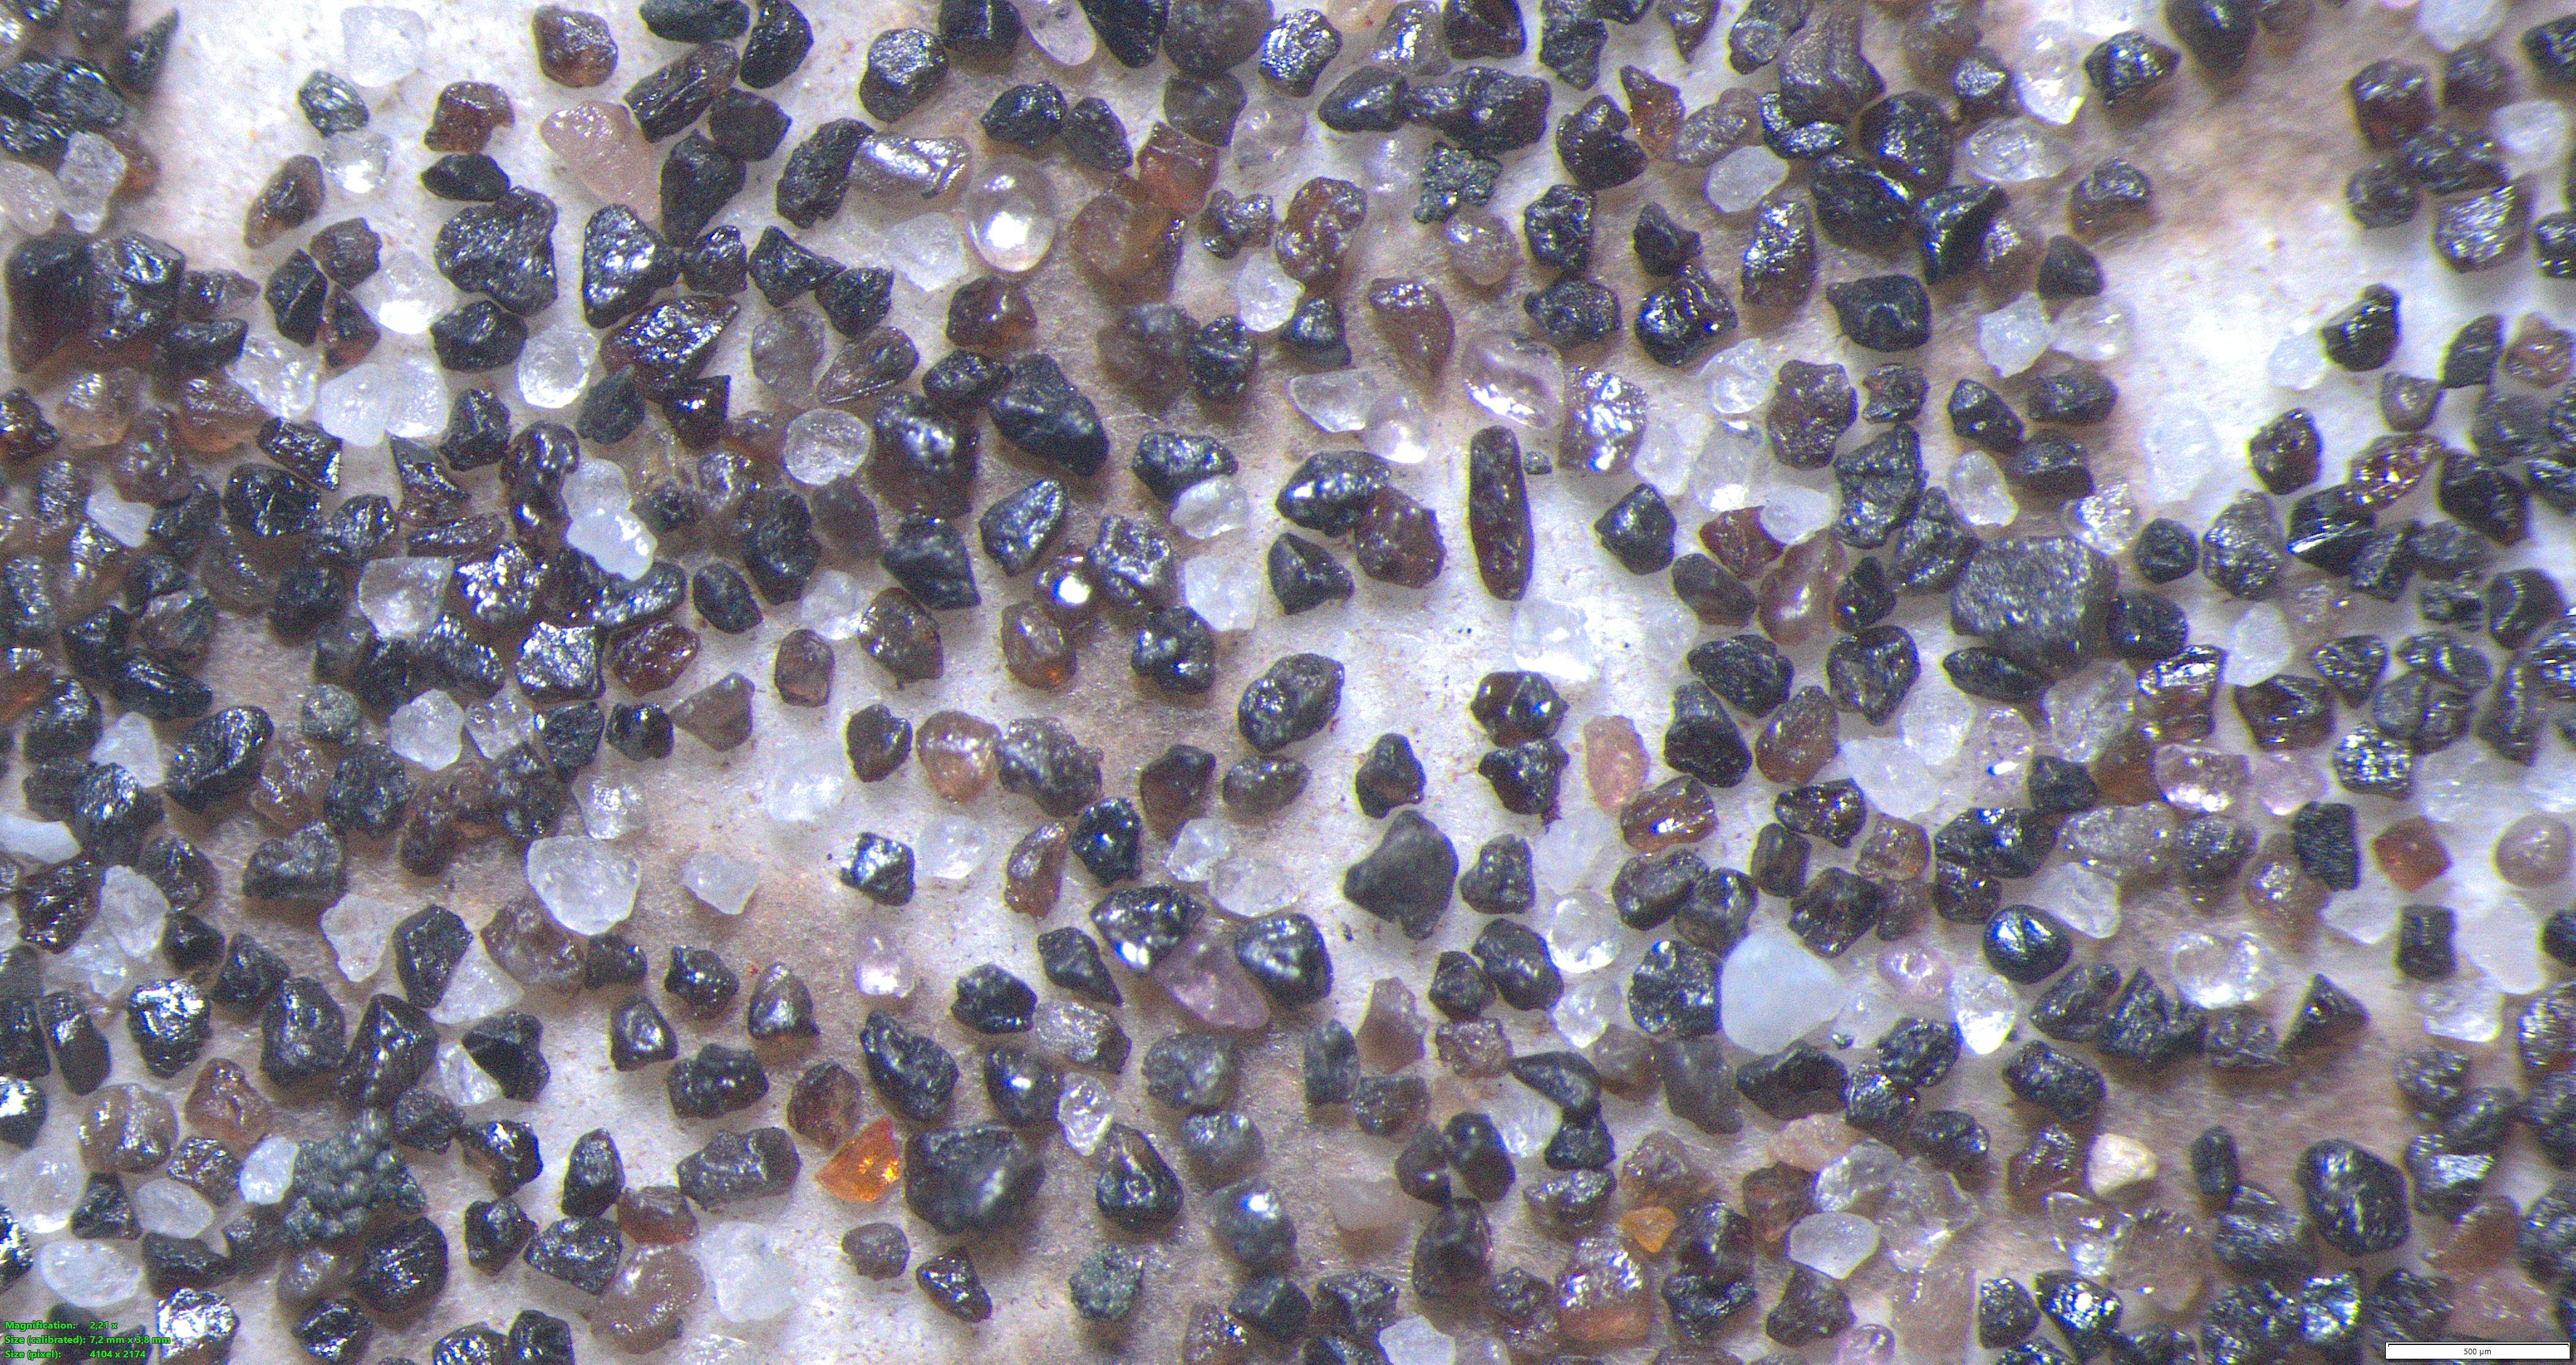
\includegraphics[width=\textwidth]{figure/segmentasiOri.jpg}
		\caption{Citra Original}
		\label{fig:2.Segmentasi1}
	\end{subfigure}
	\hspace{0.5cm}
	\begin{subfigure}[b]{0.425\textwidth}
		\centering
		
\includegraphics[width=\textwidth]{figure/segmentasiMask.png}
		\caption{Citra Hasil Segmentasi (\textit{Mask})}
		\label{fig:2.Segmentasi2}
	\end{subfigure}

	\caption{Perbandingan Hasil Segmentasi Citra}
	\label{fig:2.SegmentasiComparison}
\end{figure}

\subsubsection*{\textnormal{1. \textit{Amodal Instance Segmentation}}}
 \label{II.TeoriAmodalInstanceSegmentation}
\textit{Amodal instance segmentation} merupakan tugas untuk memprediksi wilayah yang mencakup keseluruhan bagian objek, baik yang terlihat (\textit{visible}) maupun yang terhalang atau tersembunyi (\textit{occluded}) oleh objek lain. Ini berbeda dari \textit{modal instance segmentation} standar, yang tujuannya hanya menandai piksel-piksel objek yang terlihat. Tantangan utama dalam pengembangan metode untuk tugas ini adalah kurangnya ketersediaan data latih publik yang memiliki anotasi \textit{amodal}. Meskipun demikian, sebuah sistem segmentasi \textit{amodal} yang efektif sangat penting karena memungkinkan penalaran oklusi (\textit{occlusion reasoning}) yang canggih, seperti kemampuan untuk menyimpulkan keberadaan, batasan, dan urutan kedalaman relatif dari objek yang terhalang \cite{AmodalInstanceSegmentation}. Perbandingan citra asli dengan hasil segmentasi \textit{modal} dan \textit{amodal} ditunjukkan pada Gambar \ref{fig:2.Amodal}, yang menggambarkan perbedaan area prediksi antara objek yang terlihat dan yang tersembunyi. \par

\begin{figure}[H] % Kalau menggunakan H, posisi gambar akan tepat dibawah teks
    \centering
    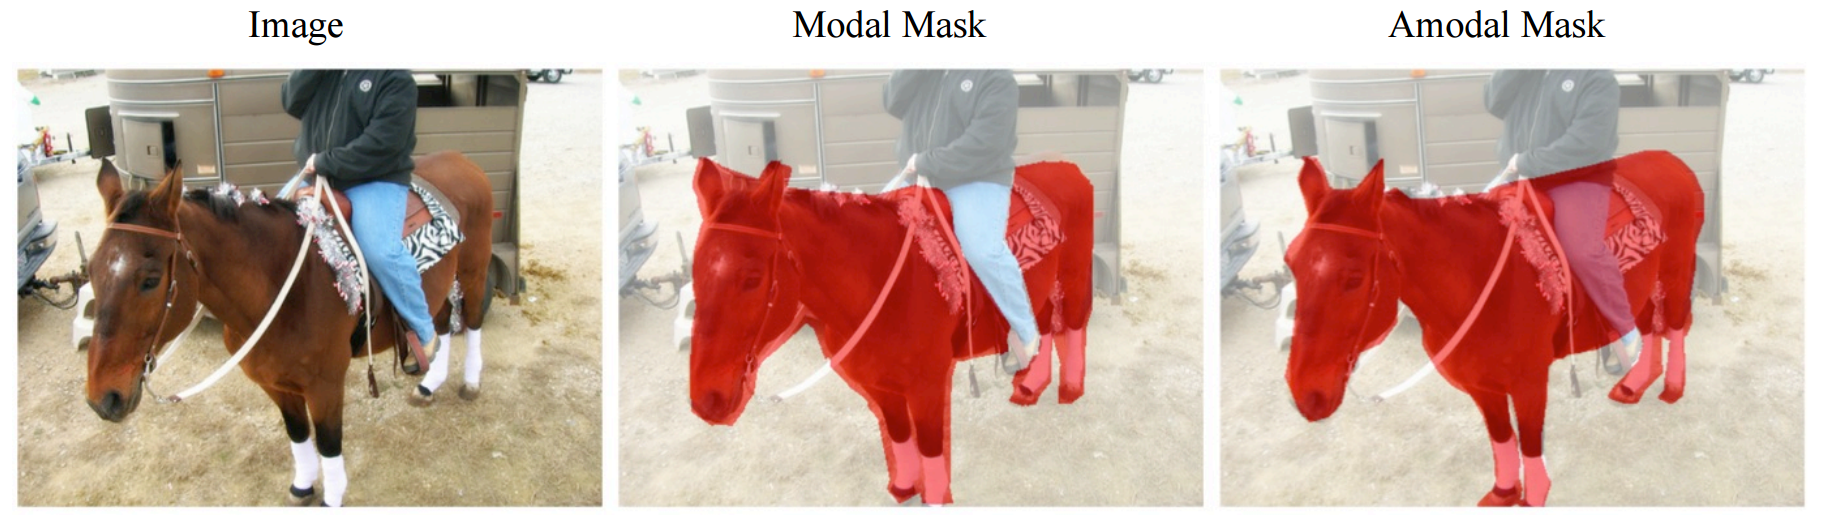
\includegraphics[width=1\textwidth]{figure/amodal.png}
    \caption{Perbandingan Hasil Segmentasi \textit{modal} dan \textit{amodal} \cite{AmodalInstanceSegmentation}}
    \label{fig:2.Amodal}
\end{figure}

\subsubsection{Pembagian Citra (\textit{Image Tiling})} \label{II.TeoriImageTiling}
Pembagian citra (\textit{image tiling}) merupakan teknik strategi pemrosesan yang membagi citra beresolusi tinggi menjadi potongan-potongan sub-citra (\textit{tiles}) yang saling tumpang tindih untuk mengatasi hilangnya detail pada deteksi objek kecil. Pendekatan ini secara efektif meningkatkan ukuran area piksel relatif objek kecil saat dimasukkan ke dalam jaringan saraf tiruan, sehingga mencegah kegagalan deteksi yang sering terjadi akibat proses \textit{down-sampling} pada arsitektur CNN standar. Metode ini diterapkan secara konsisten baik pada tahapan pelatihan (\textit{training}) untuk memperkaya representasi data, maupun pada tahapan inferensi (\textit{inference}) untuk menjaga akurasi deteksi pada perangkat dengan daya komputasi terbatas seperti GPU seluler. Akhirnya, proposal objek yang terdeteksi secara independen pada setiap potongan citra akan digabungkan kembali menggunakan algoritma merging yang memperhitungkan irisan antar-\textit{tile} untuk menghasilkan deteksi final yang akurat pada resolusi asli citra \cite{ImageTiling}.

% \subsubsection{\textit{Resize}} \label{II.TeoriResize}
% \textit{Resize image} merupakan salah satu tahap \textit{preprocessing} yang berperan untuk menyamaratakan semua gambar pada tingkat ukuran yang sama dengan ukuran yang telah ditentukan (misalnya $1920 \times 1080$) \cite{resize}. Penyesuaian  dimensi  gambar pada tahap ini memastikan bahwa semua data yang akan di input dapat diproses secara konsisten oleh model. Tujuan utama dari penyeragaman ukuran ini adalah untuk mengurangi ukuran file suatu citra dan meringankan beban kerja dari proses training data. 

\subsubsection{Augmentasi Data} \label{II.TeoriAugmentasiData}
Augmentasi data merupakan proses modifikasi gambar dalam dataset untuk menciptakan variasi baru sehingga data menjadi lebih beragam tanpa mengubah label aslinya. Teknik ini bertujuan untuk meningkatkan keragaman data pelatihan secara minimal tanpa perlu mengumpulkan data baru secara manual, yang berfungsi efektif untuk mengurangi risiko overfitting. Melalui penambahan variansi data, augmentasi membantu model mengenali pola visual dari berbagai sudut pandang dan skenario pencahayaan yang berbeda.

\subsubsection*{\textnormal{1. \textit{Flip}}} \label{II.TeoriFlip}
\textit{Flip}, atau membalik gambar, merupakan salah satu teknik manipulasi gambar yang dikategorikan sebagai metode augmentasi data dasar (\textit{basic approaches}). Teknik ini termasuk dalam metode augmentasi geometris yang umumnya diterapkan dalam dua bentuk, yaitu \textit{vertical flip} (membalik secara vertikal) dan \textit{horizontal flip} (membalik secara horizontal). Tujuan utama dari penerapan flipping adalah untuk meningkatkan jumlah dan keragaman data pelatihan secara signifikan tanpa mengubah label atau makna sebenarnya dari citra tersebut \cite{flip}. Operasi \textit{flip} dapat di lakukan menggunakan \ref{eq:2.HorizontalFlip} untuk \textit{flip} horizontal dan \ref{eq:2.VerticalFlip} untuk \textit{flip} vertikal \cite{thesisNova}. \par

\vspace{0.5\baselineskip}
\begin{equationcaptioned}[eq:2.HorizontalFlip]{
		I'(x, y) = I(W - 1 - x, y)
	}{
		Operasi \textit{Horizontal Flip}
	}
\end{equationcaptioned}

Keterangan:
\begin{itemize}
\renewcommand\labelitemi{} % menghilangkan simbol bullet
    \item $I'(x, y)$ : nilai piksel setelah dilakukan pembalikan
    \item $I(x, y)$ : nilai piksel asli
    \item $W$ : lebar citra
    \item $W - 1 - x$ : posisi kolom baru setelah dilakukan pembalikan
    \item $y$ : koordinat baris (tidak berubah)
\end{itemize}

\vspace{0.5\baselineskip}
\begin{equationcaptioned}[eq:2.VerticalFlip]{
		I'(x, y) = I(x, H - 1 - y)
	}{
		Operasi \textit{Vertical Flip}
	}
\end{equationcaptioned}

Keterangan:
\begin{itemize}
\renewcommand\labelitemi{} % menghilangkan simbol bullet
    \item $I'(x, y)$ : nilai piksel setelah dilakukan pembalikan
    \item $H$ : tinggi citra
    \item $H - 1 - y$ : posisi baris baru setelah dilakukan pembalikan
    \item $x$ : koordinat kolom (tidak berubah)
\end{itemize}

\subsubsection*{\textnormal{2. \textit{Rotate}}} \label{II.TeoriRotate}
\textit{Rotate} atau rotasi merupakan metode augmentasi data yang memutar citra pada sudut tertentu, seperti 15°, atau secara acak dalam rentang tertentu. Tujuannya adalah agar model menjadi lebih fleksibel dalam mengenali objek dari melakukan pengenalan pola visual di berbagai orientasi tanpa bergantung pada posisi aslinya. \textit{Rotate} membantu model mengenali pola yang sama meskipun tampil dari sudut pandang berbeda. Dengan demikian, teknik ini meningkatkan kemampuan generalisasi model terhadap variasi orientasi objek pada data pelatihan \cite{RotateBatik}. Operasi \textit{Rotate} dapat dilakukan menggunakan \ref{eq:2.operasi}, di mana matriks rotasi ${R}_\theta$ memutar vektor posisi ${x}$ sebesar sudut $\theta$ untuk menghasilkan posisi baru ${x}'$ setelah rotasi.\par

\vspace{0.5\baselineskip}
\begin{equationcaptioned}[eq:2.operasi]{
		{x}' = {R}_\theta \, {x}
	}{
		Operasi \textit{Rotate}
	}
\end{equationcaptioned}

Keterangan:
\begin{itemize}
\renewcommand\labelitemi{} % menghilangkan simbol bullet
	\item ${x}'$ : vektor posisi hasil rotasi setelah dilakukan perputaran sebesar sudut $\theta$
    \item ${R}_\theta$ : operator rotasi (matriks rotasi) yang memutar semua titik terhadap titik asal $(0,0)$ sebesar sudut $\theta$
    \item ${x}$ : vektor posisi awal suatu titik atau piksel sebelum rotasi
\end{itemize}

% \vspace{0.5\baselineskip}
% \begin{equationcaptioned}[eq:2.clockwise]{
% 		{R}_{\text{CW}} =
% 		\begin{bmatrix}
% 		\cos\theta & \sin\theta \\
% 		-\sin\theta & \cos\theta
% 		\end{bmatrix}
% 	}{
% 		Operasi \textit{Rotate Clockwise}
% 	}
% \end{equationcaptioned}

% Keterangan:
% \begin{itemize}
% \renewcommand\labelitemi{} % menghilangkan simbol bullet
% 	\item ${R}_{\text{CW}}$ : matriks rotasi untuk arah searah jarum jam (\textit{clockwise})
%     \item $\theta$ : sudut rotasi (dalam radian), searah jarum jam (\textit{clockwise})
% \end{itemize}

% \vspace{0.5\baselineskip}
% \begin{equationcaptioned}[eq:2.counter-clockwise]{
% 		{R}_{\text{CCW}} =
% 		\begin{bmatrix}
% 		\cos\theta & -\sin\theta \\
% 		\sin\theta & \cos\theta
% 		\end{bmatrix}
% 	}{
% 		Operasi \textit{Rotate Counter Clockwise}
% 	}
% \end{equationcaptioned}

% Keterangan:
% \begin{itemize}
% \renewcommand\labelitemi{} % menghilangkan simbol bullet
% 	\item ${R}_{\text{CCW}}$ : matriks rotasi untuk berlawanan arah jarum jam (\textit{counter-clockwise})
%     \item $\theta$ : sudut rotasi (dalam radian), berlawanan arah jarum jam (\textit{counter-clockwise})
% \end{itemize}


\subsubsection*{\textnormal{3. \textit{Gaussian Noise}}} \label{II.TeoriGaussianNoise}
\textit{Gaussian noise} adalah derau statistik (\textit{statistical noise}) yang memiliki fungsi kepadatan probabilitas (\textit{probability density function}) yang setara dengan distribusi normal. Derau ini bersifat aditif (\textit{additive noise}), di mana piksel dalam gambar yang bising (\textit{noisy image}) merupakan hasil penjumlahan dari nilai piksel asli dengan nilai \textit{Gaussian noise} acak. \textit{Gaussian noise} bersifat independen di setiap piksel dan juga independen terhadap besaran sinyal (\textit{signal magnitude}) \cite{GaussianNoiseManga}. Dalam konteks augmentasi data, Gaussian noise dapat ditambahkan ke fitur kueri (\textit{query feature}) yang diambil sampelnya dari distribusi \textit{Gaussian} untuk meningkatkan variasi kueri tersebut di dalam \textit{feature space} \cite{GaussianNoise}. Operasi \textit{Gaussian Noise} dapat di lakukan menggunakan \ref{eq:2.gaussian_distribution} untuk distribusi \textit{gaussian} pada fitur \par
% dan \ref{eq:2.gaussian_addition} untuk penambahan noise ke fitur yang hanya di lakukan pada tahap \textit{training} untuk memperbesar variasi data di ruang fitur.\par

\vspace{0.5\baselineskip}
\begin{equationcaptioned}[eq:2.gaussian_distribution]{
    n_{ijk} \sim \mathcal{N}(0, \sigma_i^2)
}{
    Distribusi \textit{Gaussian} pada Fitur
}
\end{equationcaptioned}

Keterangan:
\begin{itemize}
\renewcommand\labelitemi{} % menghilangkan simbol bullet
    \item $n_{ijk}$ : nilai \textit{noise} pada channel ke-$i$, baris ke-$j$, dan kolom ke-$k$
    \item $\sigma_i$ : standar deviasi dari \textit{noise} untuk channel ke-$i$
    \item $\mathcal{N}(0, \sigma_i^2)$ : distribusi Gaussian dengan mean $0$ dan variansi $\sigma_i^2$
\end{itemize}

% \vspace{0.5\baselineskip}
% \begin{equationcaptioned}[eq:2.gaussian_addition]{
%     {F}_q \leftarrow {F}_q + {N}
% }{
%     Penambahan \textit{Noise Gaussian} pada Fitur
% }
% \end{equationcaptioned}

% Keterangan:
% \begin{itemize}
% \renewcommand\labelitemi{} % menghilangkan simbol bullet
%     \item ${F}_q$ : fitur dari \textit{query image}
%     \item ${N}$ : tensor \textit{Gaussian noise} berukuran $C \times H \times W$
% \end{itemize}

\subsubsection{\textit{Normalization}} \label{II.TeoriNormalization}
\textit{Normalization} atau proses normalisasi adalah sebuah proses mengubah nilai piksel pada gambar ke dalam rentang tertentu, seperti melakukan konversi nilai piksel dari rentang 0--255 menjadi 0--1. Proses ini digunakan untuk mempersiapkan data agar dapat memenuhi kebutuhan pemrosesan dan mendukung model dalam mendapatkan hasil yang lebih optimal. Pentingnya proses normalisasi adalah agar input memiliki nilai yang seragam. Input data yang tidak seragam akan mempengaruhi proses komputasi dan hasil akhir pada aplikasi \cite{Normalisasi}. Operasi normalisasi piksel dapat dilakukan dengan menggunakan \ref{eq:2.normalization} \cite{thesisNova}. \par

\vspace{0.5\baselineskip}
\begin{equationcaptioned}[eq:2.normalization]{
    X_{normal} = \frac{X - X_{min}}{X_{max} - X_{min}}
}{
    Normalisasi Piksel
}
\end{equationcaptioned}

Keterangan:
\begin{itemize}
\renewcommand\labelitemi{} % menghilangkan simbol bullet
    \item $X_{normal}$ : nilai piksel setelah dilakukan normalisasi
    \item $X_{min}$ : nilai piksel minimum dalam citra (biasanya 0)
    \item $X_{max}$ : nilai piksel maksimum dalam citra (biasanya 255)
    \item $X$ : nilai piksel asli
\end{itemize}

\subsection{\textit{Deep Learning}} \label{II.TeoriDeepLearning}
\textit{Deep Learning} merupakan metode pembelajaran representasi yang menggunakan model komputasi dengan beberapa lapisan pemrosesan untuk mempelajari representasi data pada berbagai tingkat abstraksi. Metode ini memungkinkan mesin untuk diberi data mentah dan secara otomatis menemukan representasi yang diperlukan untuk deteksi atau klasifikasi. Dimulai dari input mentah, setiap modul sederhana namun \textit{non-linear} dalam lapisan tersebut mengubah representasi di satu tingkat menjadi representasi di tingkat yang lebih tinggi dan sedikit lebih abstrak \cite{DeepLearning}. \par

Untuk menemukan struktur rumit dalam kumpulan data besar, \textit{deep Learning} memanfaatkan algoritma backpropagation untuk menunjukkan bagaimana mesin harus mengubah parameter internalnya di setiap lapisan. Aspek kunci dari \textit{deep Learning} adalah bahwa lapisan-lapisan fitur ini tidak dirancang oleh insinyur manusia, melainkan dipelajari dari data menggunakan prosedur pembelajaran umum. Pendekatan ini telah secara dramatis meningkatkan kemampuan \textit{state-of-the-art} dalam berbagai \textit{domain}, termasuk klasifikasi gambar, pengenalan objek visual, deteksi objek, dan pengenalan ucapan \cite{DeepLearning} \cite{DeepResidual}. \par

\subsection{\textit{Transfer Learning}} \label{II.TeoriTransferLearning}
\textit{Transfer learning} merupakan sebuah pendekatan yang memanfaatkan pengetahuan (\textit{knowledge}) dari domain sumber untuk meningkatkan kinerja pada domain target. Pendekatan ini sering menggunakan \textit{pre-trained model}, yaitu model yang telah dilatih pada dataset berskala besar sehingga menyediakan pengetahuan dasar dan umum yang fundamental untuk tugas-tugas \textit{downstream}. Dengan memanfaatkan model yang sudah dilatih ini, sebuah paradigma yang sukses seperti \textit{fine-tuning} memungkinkan peningkatan kinerja pada tugas target tanpa harus memulai keseluruhan proses pelatihan dari awal. Karena banyaknya model yang tersedia, penilaian \textit{pre-trained model} untuk \textit{transfer learning} menjadi penting untuk mengidentifikasi kandidat model yang optimal bagi tugas \textit{downstream} tertentu \cite{TransferLearning}. \par

\subsection{\textit{Mask} R-CNN} \label{II.TeoriMaskRCNN}
\textit{Mask} R-CNN adalah sebuah kerangka kerja (\textit{framework}) yang fleksibel dan umum untuk tugas \textit{instance segmentation} objek, yang secara efisien mendeteksi objek dalam sebuah citra dan menghasilkan masker segmentasi berkualitas tinggi untuk setiap objek secara bersamaan \cite{MaskRcnnIEEE11}. Arsitektur ini merupakan perluasan dari \textit{Faster} R-CNN dengan menambahkan sebuah cabang (\textit{branch}) baru secara paralel untuk memprediksi masker objek di samping cabang yang sudah ada untuk klasifikasi kelas dan regresi \textit{bounding box} \cite{MaskRcnnIEEE11}. Alur kerja dan hubungan antar komponen utama seperti \textit{Region Proposal Network} (RPN), \textit{ROI Align}, serta cabang klasifikasi, regresi, dan prediksi masker dapat dilihat pada Gambar \ref{fig:2.MaskR-CNN}.  \par

\begin{figure}[H] % Kalau menggunakan H, posisi gambar akan tepat dibawah teks
    \centering
    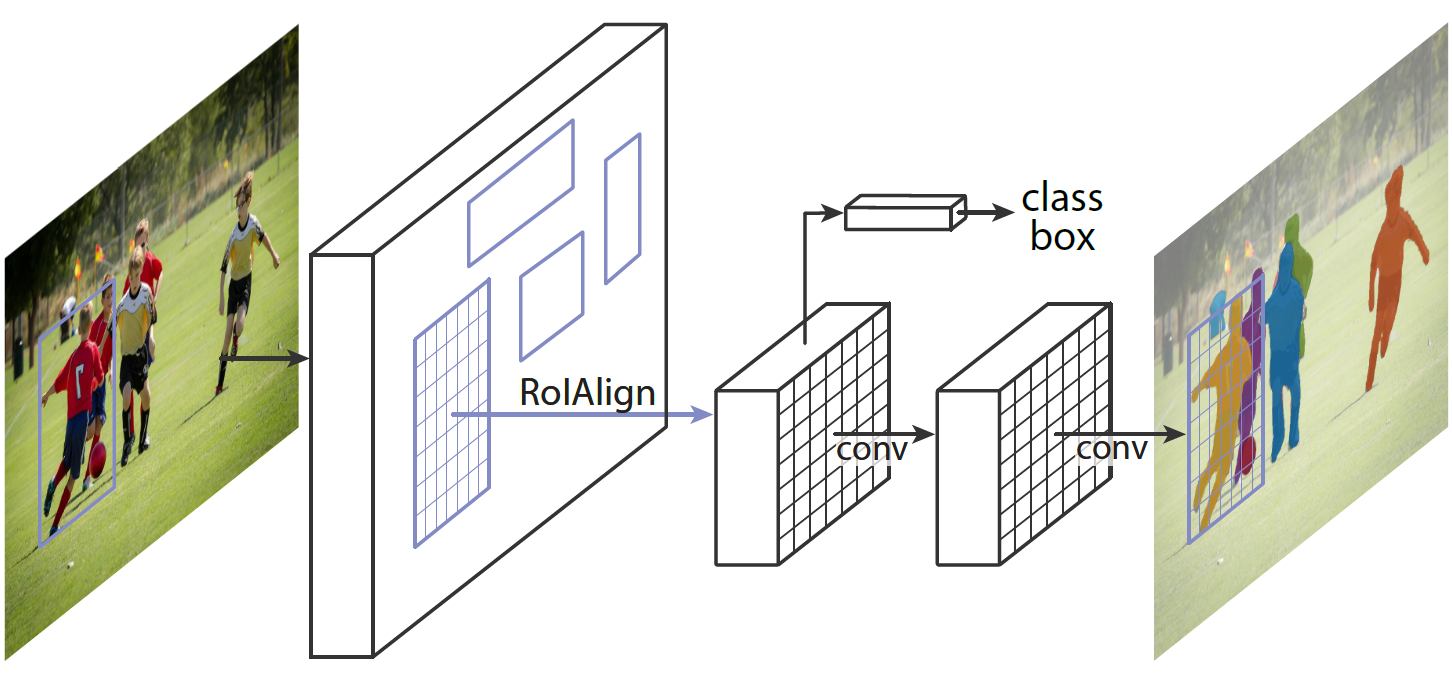
\includegraphics[width=0.8\textwidth]{figure/maskrcnn.png}
    \caption{Alur Kerja dari Arsitektur \textit{Mask} R-CNN \cite{MaskRcnnIEEE11}}
    \label{fig:2.MaskR-CNN}
\end{figure}

Pendekatan \textit{Mask} R-CNN ini mengikuti prosedur dua tahap yang sama seperti \textit{Faster} R-CNN, dimana tahap pertama adalah RPN yang mengusulkan kandidat \textit{bounding box} objek, dan tahap kedua secara paralel melakukan klasifikasi, regresi \textit{bounding box}, serta prediksi masker biner untuk setiap RoI \cite{MaskRcnnIEEE11}. Secara arsitektur, \textit{Mask} R-CNN dimulai dengan jaringan \textit{backbone} konvolusi (seperti ResNet yang dikombinasikan dengan \textit{Feature Pyramid Network} (FPN)) yang berfungsi untuk mengekstraksi fitur dari seluruh citra input. Fitur yang diekstraksi kemudian diteruskan ke RPN untuk menghasilkan sejumlah kandidat RoI \cite{MaskRcnnIEEE11}. Setiap RoI diproses melalui lapisan RoIAlign guna menjaga keselarasan spasial sebelum diteruskan ke tiga cabang paralel untuk klasifikasi objek, regresi \textit{bounding box}, dan prediksi masker biner berukuran $m \times m$ untuk setiap kelas objek \cite{MaskRcnnIEEE11}. Fungsi kerugian total (\textit{loss function}) pada \textit{Mask} R-CNN dapat dilihat pada \ref{eq:2.maskrcnn} \cite{MaskRcnnIEEE11}, yang merupakan gabungan dari tiga komponen kerugian utama. Perhitungan \textit{classification loss} secara spesifik ditunjukkan pada Persamaan~\ref{eq:2.cls_loss}, sedangkan perhitungan \textit{bounding box regression loss} dijelaskan pada Persamaan~\ref{eq:2.box_loss}, dan perhitungan \textit{mask loss} secara spesifik dijelaskan pada \ref{eq:2.maskloss} \cite{rumusMaskrcnn} berikut. \par

\vspace{0.5\baselineskip}
\begin{equationcaptioned}[eq:2.maskrcnn]{
	L = L_{\text{cls}} + L_{\text{box}} + L_{\text{mask}}
}{
	Fungsi Loss \textit{Mask} R-CNN
}
\end{equationcaptioned}

Keterangan:
\begin{itemize}
\renewcommand\labelitemi{} % menghilangkan simbol bullet
	\item \(L_{\text{cls}}\) : \textit{classification loss} untuk memprediksi kelas objek.
	\item \(L_{\text{box}}\) : \textit{bounding box regression loss} untuk memperkirakan posisi kotak pembatas.
	\item \(L_{\text{mask}}\) : \textit{mask loss} berbasis \textit{binary cross-entropy} yang dihitung per piksel pada setiap \textit{Region of Interest (RoI)}.
\end{itemize}

\vspace{0.5\baselineskip}
\begin{equationcaptioned}[eq:2.cls_loss]{
    {L}_{cls}
    = \frac{1}{N_{cls}} \sum_i \big(-p_i^* \log p_i - (1 - p_i^*) \log (1 - p_i)\big)
}{
    Fungsi kerugian klasifikasi (\textit{Classification Loss})
}
\end{equationcaptioned}

Keterangan:
\begin{itemize}
\renewcommand\labelitemi{} % menghilangkan simbol bullet
    \item ${L}_{cls}$ : \textit{Classification loss}, menghitung kesalahan antara hasil klasifikasi ($p_i$) dan label sebenarnya ($p_i^*$).
    \item $N_{cls}$ : Jumlah total \textit{anchor} yang digunakan untuk proses klasifikasi.
    \item $p_i$ : Probabilitas prediksi bahwa \textit{anchor} ke-$i$ mengandung objek (output dari \textit{sigmoid classifier}).
    \item $p_i^*$ : Label kebenaran untuk \textit{anchor} ke-$i$ ($1$ jika mengandung objek, $0$ jika bukan objek).
\end{itemize}

\vspace{0.5\baselineskip}
\begin{equationcaptioned}[eq:2.box_loss]{
    {L}_{box}
    = \frac{\lambda}{N_{box}} \sum_i p_i^* \cdot L_1^{smooth}(t_i - t_i^*)
}{
    Fungsi kerugian regresi kotak pembatas (\textit{Bounding Box Regression Loss})
}
\end{equationcaptioned}

Keterangan:
\begin{itemize}
\renewcommand\labelitemi{} % menghilangkan simbol bullet
    \item ${L}_{box}$ : \textit{Bounding box regression loss}, mengukur perbedaan antara koordinat prediksi ($t_i$) dan koordinat sebenarnya ($t_i^*$).
    \item $N_{box}$ : Jumlah total \textit{anchor} yang digunakan untuk regresi kotak pembatas.
    \item $t_i$ : Vektor koordinat prediksi kotak pembatas hasil regresi.
    \item $t_i^*$ : Vektor koordinat sebenarnya dari kotak pembatas (\textit{ground truth box}).
    \item $\lambda$ : Koefisien penyeimbang antara kerugian klasifikasi dan regresi.
    \item $L_1^{smooth}$ : \textit{Smooth L1 loss}, fungsi yang digunakan untuk menghitung selisih koordinat secara stabil tanpa pengaruh ekstrem.
\end{itemize}

\vspace{0.5\baselineskip}
\begin{equationcaptioned}[eq:2.maskloss]{
	L_{\text{mask}} = -\frac{1}{m^2}\sum_{1 \leq i,j \leq m}
	\Big[ y_{ij} \log \hat{y}^{k}_{ij} + (1 - y_{ij}) \log (1 - \hat{y}^{k}_{ij}) \Big]
}{
	Operasi \textit{Mask Loss (Binary Cross-Entropy)}
}
\end{equationcaptioned}

Keterangan:
\begin{itemize}
\renewcommand\labelitemi{}
	\item $m$² atau $m \times m$ : ukuran resolusi keluaran \textit{mask} untuk setiap kelas objek.
	\item $y_{ij}$ : nilai \textit{ground-truth} piksel ke-$i,j$ (1 untuk area objek, 0 untuk latar belakang).
	\item $\hat{y}^{k}_{ij}$ : probabilitas hasil prediksi piksel ke-$i,j$ untuk kelas objek ke-$k$.
	\item Operasi penjumlahan $\sum_{1 \leq i,j \leq m}$ : menghitung rata-rata \textit{binary cross-entropy loss} dari seluruh piksel pada mask.
\end{itemize}

\subsubsection{\textit{Backbone}} \label{II.TeoriBackbone}
\textit{Backbone} merupakan jaringan konvolusi dasar yang berfungsi mengekstraksi fitur dari seluruh citra sebelum digunakan oleh komponen lain seperti RPN atau \textit{head} deteksi. Salah satu arsitektur yang umum digunakan sebagai \textit{backbone} adalah ResNet-50 (\textit{Residual Network} dengan 50 lapisan), yang memperkenalkan konsep \textit{residual learning} melalui koneksi pintas (\textit{skip connection}) untuk mengatasi masalah degradasi akurasi pada jaringan yang sangat dalam. ResNet-50 terdiri dari lima tahap konvolusi dengan berbagai kedalaman lapisan residual, yang memungkinkan jaringan untuk mempelajari representasi fitur hierarkis dari tingkat rendah hingga tingkat tinggi. Ketika dikombinasikan dengan FPN, ResNet-50 menghasilkan peta fitur multi-skala yang kaya semantik, sehingga meningkatkan kemampuan deteksi dan segmentasi objek pada berbagai ukuran \cite{DeepResidual}. \par

\subsubsection{\textit{Feature Pyramid Network} (FPN)} \label{II.TeoriFPN}
\textit{Feature Pyramid Network} (FPN) merupakan arsitektur yang dirancang untuk memanfaatkan hierarki fitur multi-skala pada jaringan konvolusi (\textit{backbone}) guna membentuk piramida fitur dengan makna semantik yang konsisten di setiap tingkat skala, namun dengan biaya komputasi yang rendah \cite{fpn}. FPN menggabungkan fitur beresolusi rendah yang kaya semantik dari lapisan dalam dengan fitur beresolusi tinggi yang detail secara spasial dari lapisan dangkal melalui jalur \textit{top-down} dengan \textit{upsampling} dan koneksi lateral menggunakan konvolusi $1 \times 1$ serta penjumlahan \textit{element-wise} \cite{fpn}. Struktur umum dari arsitektur FPN dapat dilihat pada Gambar \ref{fig:2.FPN} yang memperlihatkan alur pembentukan piramida fitur melalui proses \textit{top-down} dan koneksi lateral \cite{fpn}. Fungsi matematis dari arsitektur FPN yang digunakan untuk menentukan level piramida fitur setiap RoI ditunjukkan pada Persamaan \ref{eq:2.fpn}, yang merepresentasikan hubungan antara ukuran objek dengan level \textit{feature map} yang sesuai dalam struktur piramida multi-skala.
\par

\begin{figure}[H] % Kalau menggunakan H, posisi gambar akan tepat dibawah teks
    \centering
    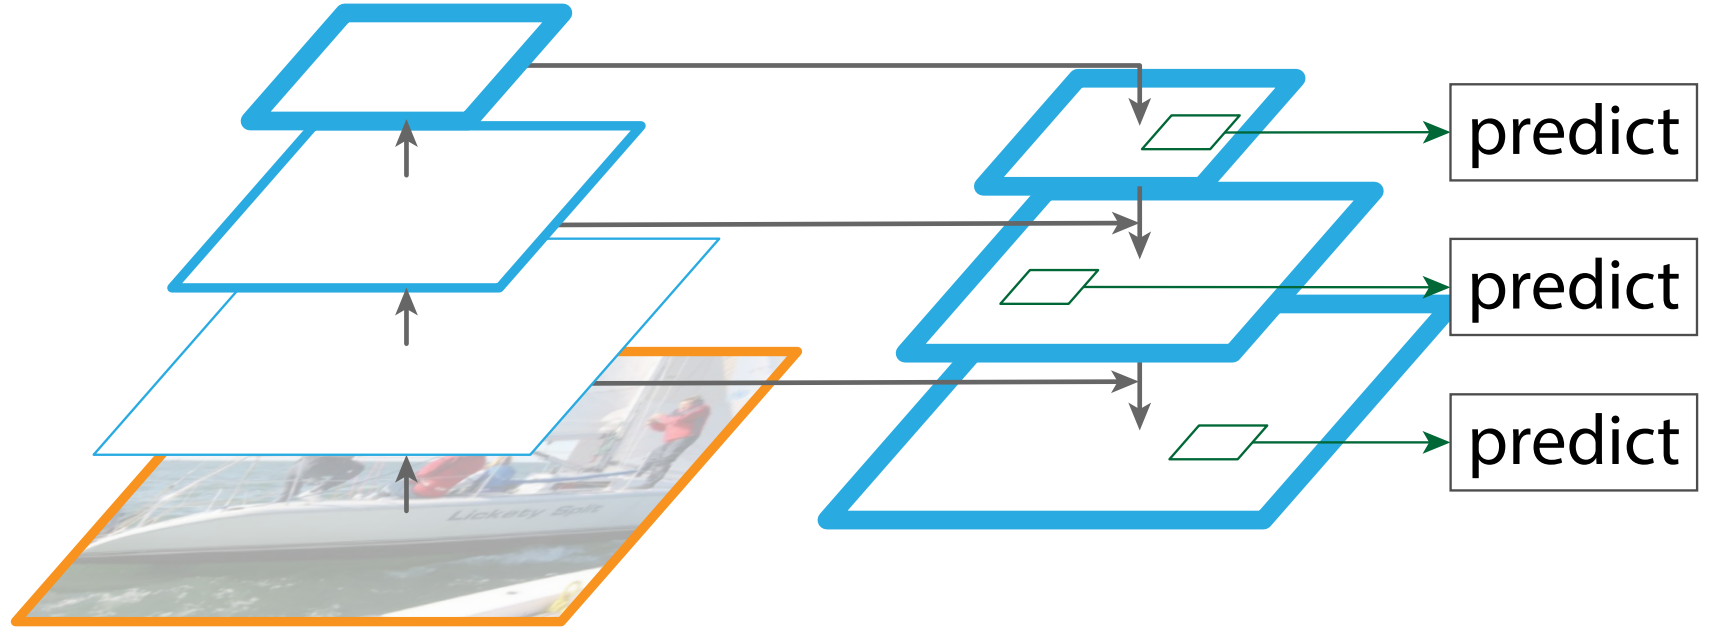
\includegraphics[width=0.8\textwidth]{figure/fpn.png}
    \caption{Arsitektur dari \textit{Feature Pyramid Network} (FPN) \cite{fpn}}
    \label{fig:2.FPN}
\end{figure}

\vspace{0.5\baselineskip}
\begin{equationcaptioned}[eq:2.fpn]{
	k = \left\lfloor k_0 + \log_2\left(\frac{\sqrt{wh}}{224}\right) \right\rfloor
}{
	Operasi Penentuan Level Piramida FPN
}
\end{equationcaptioned}

Keterangan:
\begin{itemize}
\renewcommand\labelitemi{} % menghilangkan simbol bullet
	\item $k$ : level \textit{feature map} piramida ($P_k$) tempat RoI ditempatkan.
	\item $k_0$ : level dasar piramida (biasanya $k_0 = 4$).
	\item $w, h$ : lebar dan tinggi RoI pada citra masukan.
	\item $224$ : ukuran kanonis (\textit{canonical scale}) dari \textit{ImageNet pre-training}, digunakan sebagai skala referensi.
\end{itemize}

% \subsubsection*{\textnormal{1. \textit{Multipath Feature Pyramid Network} (MFPN)}}
%  \label{II.TeoriMFPN}
% \textit{Multipath Feature Pyramid Network} (MFPN) adalah arsitektur jaringan yang diusulkan untuk mengatasi masalah kesalahan identifikasi akibat hilangnya detail fitur lapisan dalam (\textit{deep features}) selama proses ekstraksi fitur. Jaringan ini bekerja dengan menambahkan satu jalur fusi fitur (\textit{feature fusion}) baru dengan arah dari bawah ke atas (\textit{bottom-up}). Jalur baru ini beroperasi secara paralel dengan jalur fusi \textit{top-down} dari FPN orisinal, di mana fitur dari lapisan dangkal (\textit{shallow features}) akan di-downsampling dan ditambahkan ke fitur pada lapisan yang lebih dalam. Fusi dua arah yang paralel ini bertujuan untuk memperkaya informasi detail pada fitur lapisan dalam, sehingga memperkuat kemampuan jaringan dalam mengekstraksi fitur dan meningkatkan akurasi deteksi secara keseluruhan \cite{ImprovedMaskRCNNOrePanggangan}. Struktur umum dari arsitektur MFPN ditunjukkan pada Gambar \ref{fig:2.MFPN}, yang menggabungkan jalur \textit{top-down} dan \textit{bottom-up} secara paralel untuk memperkaya representasi fitur multi-skala melalui proses fusi dua arah yang meningkatkan ketepatan ekstraksi fitur pada lapisan dalam \cite{ImprovedMaskRCNNOrePanggangan}.

% \begin{figure}[H] % Kalau menggunakan H, posisi gambar akan tepat dibawah teks
%     \centering
%     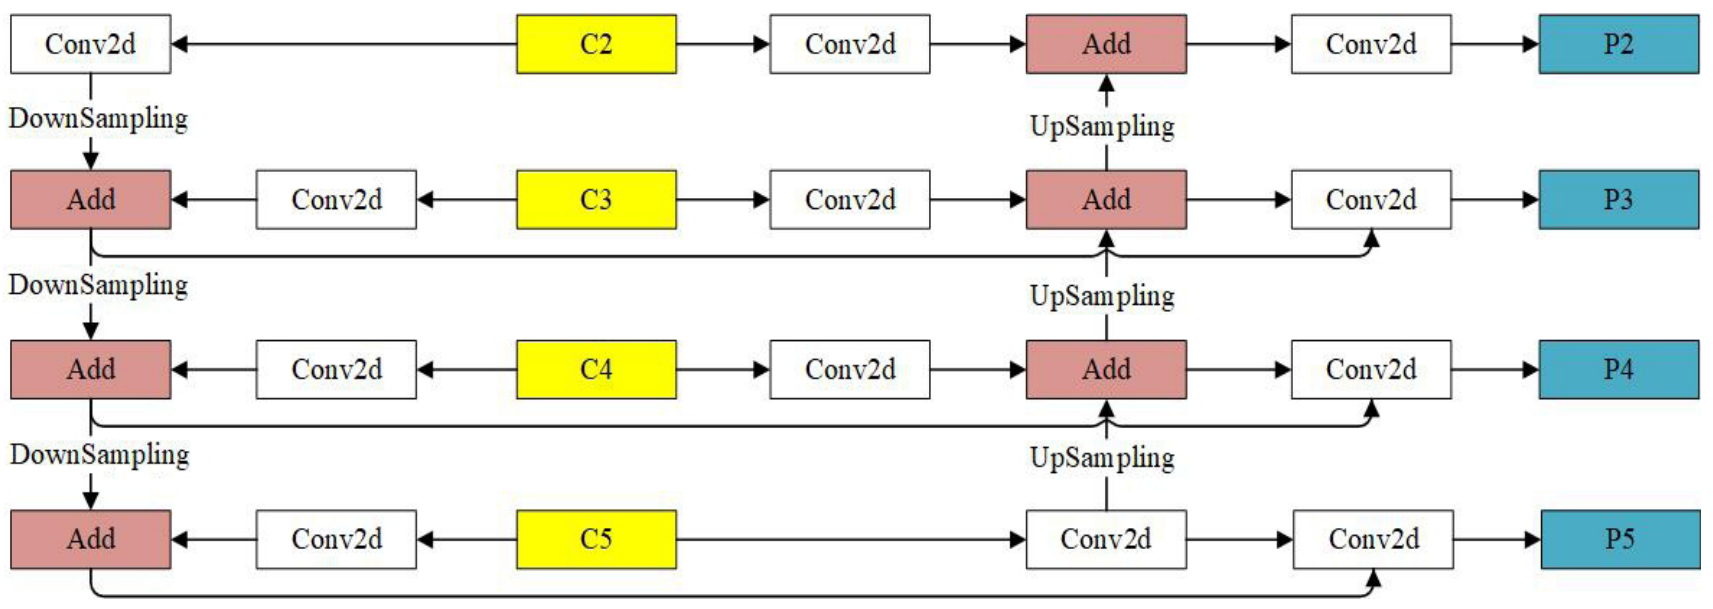
\includegraphics[width=1\textwidth]{figure/MFPN.png}
%     \caption{Struktur Arsitektur \textit{Multipath Feature Pyramid Network} (MFPN) \cite{ImprovedMaskRCNNOrePanggangan}}
%     \label{fig:2.MFPN}
% \end{figure}

\subsubsection{\textit{Region Proposal Network} (RPN)} \label{II.TeoriRPN}
\textit{Region Proposal Network} (RPN) adalah sebuah Jaringan Konvolusi Penuh (\textit{Fully Convolutional Network}) yang diperkenalkan untuk mengatasi hambatan komputasi dalam menghasilkan proposal wilayah pada sistem deteksi objek. RPN bekerja dengan cara berbagi lapisan konvolusi full-image dengan jaringan deteksi utama, sehingga memungkinkan proses penghasilan proposal wilayah menjadi hampir tanpa biaya (\textit{nearly cost-free}). Jaringan ini, seperti yang diilustrasikan pada Gambar \ref{fig:2.RPN}, secara bersamaan memprediksi batas-batas objek (\textit{object bounds}) dan skor keobjekan (\textit{objectness scores}) pada setiap posisi di peta fitur konvolusi. RPN dilatih secara \textit{end-to-end} untuk menghasilkan proposal wilayah berkualitas tinggi yang kemudian digunakan oleh jaringan deteksi untuk melakukan deteksi objek \cite{RPN}. Fungsi kerugian (\textit{loss function}) RPN yang digunakan untuk optimasi jaringan ditunjukkan pada Persamaan \ref{eq:RPNLoss}, yang menggabungkan komponen klasifikasi dan regresi untuk setiap \textit{anchor} yang diproses \cite{RPN}. \par

\begin{figure}[H] % Kalau menggunakan H, posisi gambar akan tepat dibawah teks
    \centering
    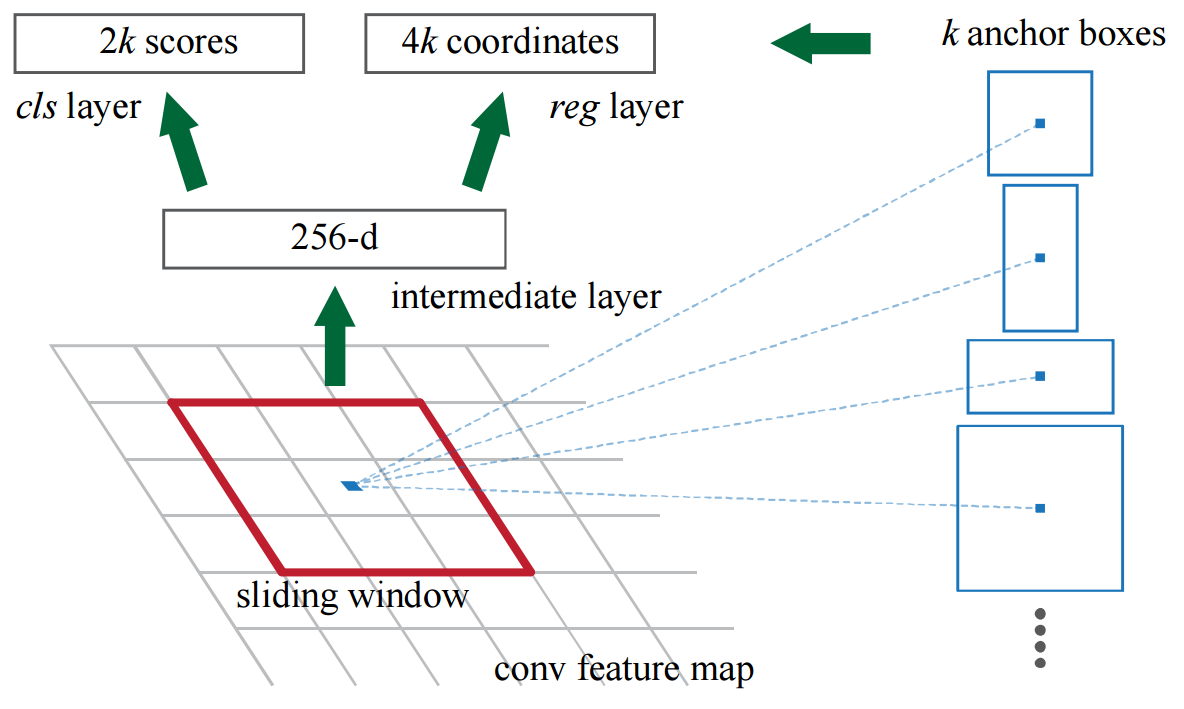
\includegraphics[width=0.8\textwidth]{figure/RPN.png}
    \caption{Jaringan dari \textit{Region Proposal Network} (RPN) \cite{RPN}}
    \label{fig:2.RPN}
\end{figure}

\vspace{0.5\baselineskip}
\begin{equationcaptioned}[eq:RPNLoss]{
    L(\{p_i\}, \{t_i\}) =
    \frac{1}{N_{\text{cls}}} \sum_i L_{\text{cls}}(p_i, p_i^*)
    + \lambda \frac{1}{N_{\text{reg}}} \sum_i p_i^* L_{\text{reg}}(t_i, t_i^*)
}{
    Fungsi Kerugian \textit{loss function} RPN
}
\end{equationcaptioned}

Keterangan:
\begin{itemize}
\renewcommand\labelitemi{} % menghilangkan simbol bullet
    \item $L_{\text{cls}}$ : \textit{Binary Cross-Entropy Loss} yang digunakan untuk membedakan antara \textit{anchor} yang mengandung objek dan yang tidak.
    \item $L_{\text{reg}}$ : \textit{Smooth L1 Loss} yang mengukur perbedaan antara koordinat kotak prediksi dan \textit{ground truth}.
    \item $p_i$ : probabilitas bahwa \textit{anchor} ke-$i$ berisi objek.
    \item $p_i^*$ : label kebenaran untuk \textit{anchor} ke-$i$ (1 jika positif, 0 jika negatif).
    \item $t_i$ : vektor parameter regresi $(t_x, t_y, t_w, t_h)$ hasil prediksi RPN.
    \item $t_i^*$ : vektor target regresi yang dihitung dari selisih antara \textit{anchor} dan \textit{ground truth box}.
    \item $N_{\text{cls}}$ : jumlah total \textit{anchor} dalam satu \textit{mini-batch}.
    \item $N_{\text{reg}}$ : jumlah \textit{anchor} positif yang digunakan untuk regresi.
    \item $\lambda$ : koefisien penyeimbang antara komponen klasifikasi dan regresi (biasanya bernilai 10).
    \item $\sum_i$ : operator penjumlahan yang dilakukan terhadap seluruh \textit{anchor} ke-$i$ pada citra, baik yang berlabel positif maupun negatif.
\end{itemize}
\vspace{0.5\baselineskip}

\subsubsection{\textit{RoIAlign}} \label{II.TeoriRoIAlign}
RoIAlign adalah sebuah lapisan bebas kuantisasi yang dirancang untuk menyelaraskan fitur yang diekstraksi secara tepat dengan input. Prinsip kerjanya adalah menghindari kuantisasi kasar pada koordinat batas-batas RoI ataupun \textit{bin}, misalnya dengan menggunakan $x/16$. Lapisan ini menggunakan \textit{interpolasi bilinear} untuk menghitung nilai-nilai pasti dari fitur input pada empat lokasi sampel yang teratur di dalam setiap \textit{bin} RoI. Nilai-nilai yang dihasilkan kemudian diagregasi (biasanya menggunakan \textit{average} atau \textit{max pooling}) untuk memastikan bahwa fitur yang diekstraksi mempertahankan lokasi spasial yang tepat dan akurat \cite{MaskRcnnIEEE11}. Setiap nilai fitur pada titik $(x, y)$ di dalam \textit{bin} RoI diperoleh dengan menggabungkan empat piksel terdekat secara berbobot menurut jaraknya, yang secara matematis ditunjukkan pada Persamaan~\ref{eq:2.RoIAlign}.


\vspace{0.5\baselineskip}
\begin{equationcaptioned}[eq:2.RoIAlign]{
    y(p) = \sum_{i=0}^{1} \sum_{j=0}^{1} (1 - |x - x_i|)\,(1 - |y - y_j|)\,x(p_{ij})
}{
    Fungsi Interpolasi Bilinear pada \textit{RoIAlign}
}
\end{equationcaptioned}

Keterangan:
\begin{itemize}
\renewcommand\labelitemi{} % menghilangkan simbol bullet
    \item $y(p)$ : nilai fitur hasil \textit{sampling} di titik $(x, y)$ di dalam setiap \textit{bin} RoI.
    \item $x(p_{ij})$ : nilai fitur pada empat piksel terdekat pada \textit{feature map}.
    \item $(x_i, y_j)$ : koordinat piksel integer terdekat terhadap titik $(x, y)$.
    \item $(1 - |x - x_i|)(1 - |y - y_j|)$ : bobot \textit{interpolasi bilinear} yang menentukan kontribusi setiap piksel tetangga.
    \item $\sum_{i=0}^{1} \sum_{j=0}^{1}$ : operasi penjumlahan terhadap empat piksel terdekat untuk mendapatkan nilai fitur interpolasi.
\end{itemize}
\vspace{0.5\baselineskip}

\subsection{\textit{Optimizer}} \label{II.TeoriOptimizer}
\textit{Optimizer} merupakan salah satu komponen matematis utama dalam deep learning yang bertujuan untuk meminimalkan perbedaan antara keluaran yang diharapkan (\textit{expected output}) dan keluaran yang diinginkan (\textit{desired one}), yang diukur melalui \textit{loss function} (fungsi kerugian) \cite{optimizer}. \textit{Optimizer} mencapai tujuan ini secara iteratif dengan mengadaptasi dan memperbarui \textit{weights} (bobot) jaringan berdasarkan nilai kerugian (\textit{loss}) yang dihitung, sebuah proses yang memperkuat algoritma \textit{back-propagation}. Pemilihan \textit{optimizer} yang tepat merupakan keputusan penting karena sangat menentukan kecepatan pelatihan model \textit{deep learning} dan performa akhir yang akan diprediksi oleh model tersebut \cite{optimizer}. \par

% \subsection{\textit{Amodal Segmentation Network} (ASN)} \label{II.TeoriASN}
% \textit{Amodal Segmentation Network} (ASN) merupakan perluasan arsitektur \textit{multi-task} untuk memprediksi bentuk lengkap instan dengan menggabungkan fitur kotak (\textit{box}) dan fitur oklusi (\textit{occlusion}). Jaringan ini memperkenalkan cabang klasifikasi oklusi (\textit{occlusion classification branch}) untuk secara khusus menentukan apakah oklusi ada di dalam \textit{Region of Interest} (RoI). ASN kemudian menggunakan modul \textit{Multi-Level Coding} (MLC) untuk memperkuat informasi global tersebut, menggabungkannya dengan fitur \textit{mask} lokal untuk memandu prediksi segmentasi agar dapat merekonstruksi bagian yang terhalang \cite{AmodalASN}. Struktur umum dari arsitektur \textit{Amodal Segmentation Network} (ASN) dapat dilihat pada Gambar \ref{fig:2.ASN}, yang menunjukkan proses \textit{multi-task} dari ekstraksi fitur hingga segmentasi \textit{amodal} dan \textit{inmodal} \cite{AmodalASN}. Fungsi kerugian total (\textit{loss function}) pada ASN dapat dilihat pada \ref{eq:2.asnloss}, yang merupakan gabungan dari empat komponen kerugian utama. Perhitungan \textit{occlusion loss} secara spesifik ditunjukkan pada Persamaan~\ref{eq:occlusion_loss}, sedangkan perhitungan \textit{mask loss} dijelaskan pada \ref{eq:2.asnmask} berikut. \par

% \begin{figure}[H] % Kalau menggunakan H, posisi gambar akan tepat dibawah teks
%     \centering
%     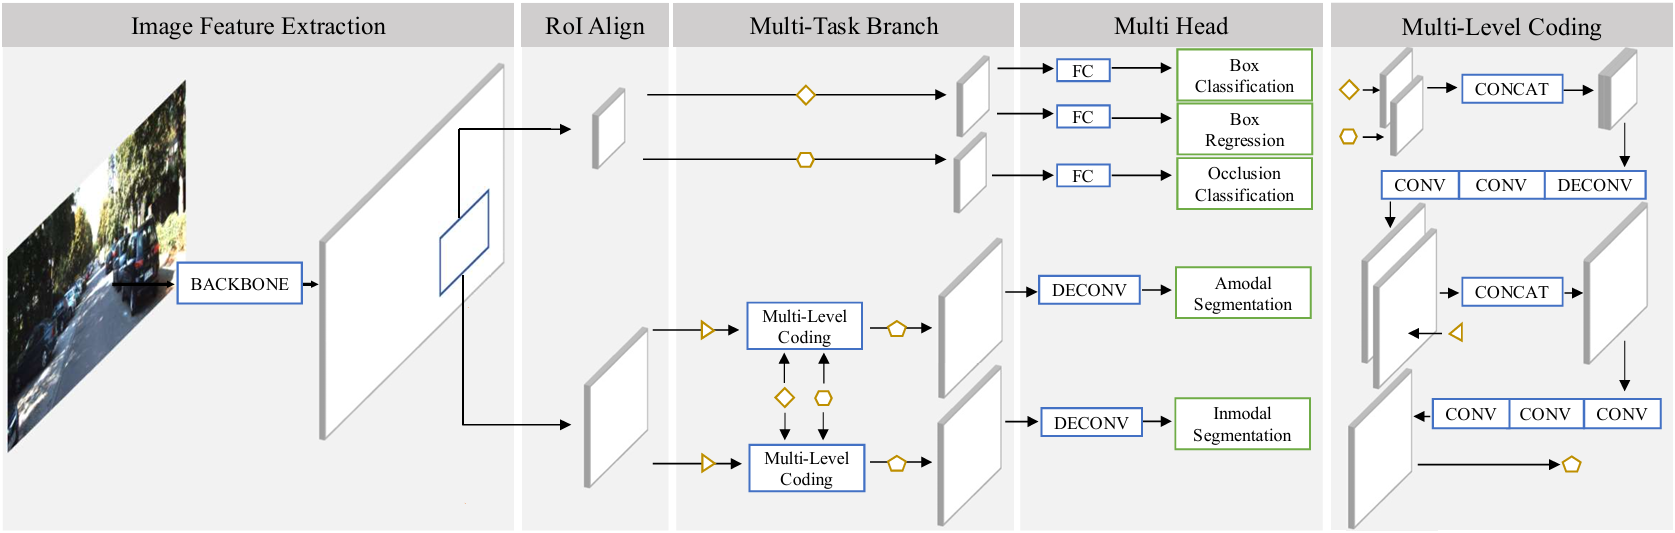
\includegraphics[width=1\textwidth]{figure/asn.png}
%     \caption{Arsitektur ASN hasil modifikasi dari \textit{Mask} R-CNN \cite{AmodalASN}}
%     \label{fig:2.ASN}
% \end{figure}

% \vspace{0.1\baselineskip}
% \begin{equationcaptioned}[eq:2.asnloss]{
% 	L = L_{\text{cls}} + L_{\text{box}} + L_{\text{occlusion}} + L_{\text{mask}}
% }{
% 	Fungsi \textit{Loss} Utama pada ASN
% }
% \end{equationcaptioned}

% Keterangan:
% \begin{itemize}
% \renewcommand\labelitemi{} % menghilangkan bullet
% 	\item \(L_{\text{cls}}\) : \textit{classification loss} untuk memprediksi kelas objek.
% 	\item \(L_{\text{box}}\) : \textit{bounding box regression loss} untuk memperkirakan posisi kotak pembatas.
% 	\item \(L_{\text{occlusion}}\) : \textit{occlusion classification loss} untuk mengenali area tertutup pada citra.
% 	\item $ L_{\text{mask}} $ : penjumlahan dari \textit{binary cross-entropy mask amodal} dan \textit{inmodal}.
% \end{itemize}

% \vspace{0.5\baselineskip}
% \begin{equationcaptioned}[eq:occlusion_loss]{
%     {L}_{occlusion}
%     = -\big[y_{occ} \log(\hat{y}_{occ}) + (1 - y_{occ}) \log(1 - \hat{y}_{occ})\big]
% }{
%     Fungsi kerugian oklusi (\textit{Occlusion Loss})
% }
% \end{equationcaptioned}

% Keterangan:
% \begin{itemize}
% \renewcommand\labelitemi{} % menghilangkan simbol bullet
%     \item ${L}_{occlusion}$ : \textit{Occlusion loss}, mengukur kesalahan klasifikasi dalam menentukan apakah suatu objek tertutupi sebagian (\textit{occluded}) atau terlihat penuh (\textit{visible}).
%     \item $y_{occ}$ : Label kebenaran untuk status oklusi, bernilai $1$ jika objek tertutupi sebagian dan $0$ jika terlihat penuh.
%     \item $\hat{y}_{occ}$ : Nilai probabilitas prediksi model terhadap status oklusi.
%     \item $\log$ : Fungsi logaritma natural yang digunakan untuk menghitung \textit{binary cross-entropy loss}.
% \end{itemize}


% \vspace{0.5\baselineskip}
% \begin{equationcaptioned}[eq:2.asnmask]{
% 	L_{\text{mask}} = L_{\text{mask}}^{a} + L_{\text{mask}}^{i}
% }{
% 	Fungsi \textit{Loss Mask} pada \textit{Amodal} dan \textit{Inmodal Segmentation}
% }
% \end{equationcaptioned}

% Keterangan:
% \begin{itemize}
% \renewcommand\labelitemi{}
% 	\item \(L_{\text{mask}}^{a}\) : \textit{mask loss} untuk segmentasi \textit{amodal} (seluruh bentuk objek).
% 	\item \(L_{\text{mask}}^{i}\) : \textit{mask loss} untuk segmentasi \textit{inmodal} (bagian yang terlihat).
% \end{itemize}

\subsection{\textit{K-Fold Cross Validation}} \label{II.TeoriKFold}
\textit{K-Fold Cross Validation} merupakan sebuah teknik intensif komputasi yang menggunakan semua contoh data yang tersedia, baik sebagai data latih \textit{(train)} maupun data uji \textit{(test)}. Prosedur ini meniru penggunaan \textit{training} dan \textit{test set} dengan melatih algoritma secara berulang sebanyak $K$ kali, di mana setiap kalinya $1/K$ bagian dari data latih disisihkan untuk pengujian \cite{kfold}. Secara praktis, data akan dibagi menjadi $K$ bagian yang terpisah, lalu secara bergantian, satu bagian dipakai untuk tes sementara bagian lainnya dipakai untuk melatih model. Ilustrasi dari \textit{k-fold cross validation} ditampilkan pada Tabel \ref{table:2.KFold}. Hasil akhirnya adalah nilai rata-rata dari semua error yang didapat dari $K$ kali proses pengujian tersebut \cite{kfold}. \par

\begin{table}[H]
\centering
\caption{Ilustrasi \textit{K-Fold Cross Validation}}
\label{table:2.KFold}
\begin{tabular}{|c|c|c|c|c|c|}
\hline
\multirow{2}{*}{\textbf{Iterasi}} & \multicolumn{5}{c|}{\textbf{\textit{K-Fold Cross Validation}}} \\
\cline{2-6}
& \textbf{Fold 1} & \textbf{Fold 2} & \textbf{Fold 3} & \textbf{Fold 4} & \textbf{Fold 5} \\
\hline
1 & \cellcolor{blue!20}\textbf{Test} & Train & Train & Train & Train \\
\hline
2 & Train & \cellcolor{blue!20}\textbf{Test} & Train & Train & Train \\
\hline
3 & Train & Train & \cellcolor{blue!20}\textbf{Test} & Train & Train \\
\hline
4 & Train & Train & Train & \cellcolor{blue!20}\textbf{Test} & Train \\
\hline
5 & Train & Train & Train & Train & \cellcolor{blue!20}\textbf{Test} \\
\hline
\end{tabular}
\end{table}

\subsection{\textit{Average Precision} (AP)} \label{II.TeoriAP}
\textit{Average Precision} (AP) merupakan metrik \textit{de-facto} yang digunakan untuk mengevaluasi kinerja deteksi objek dan segmentasi objek \cite{APmAP}. Secara fundamental, metrik AP dihitung dengan mengukur luas area di bawah kurva \textit{precision-recall detector}, yang secara matematis dapat diekspresikan sebagaimana ditunjukkan pada \ref{eq:2.AP} \cite{ap}. Perhitungan ini mengharuskan setiap prediksi objek memiliki nilai kepercayaan \textit{(confidence value)}, karena evaluasi didasarkan pada pengurutan seluruh prediksi berdasarkan skor kepercayaan tersebut. Sifat metrik ini adalah \textit{rank-sensitive} atau sensitif terhadap peringkat, yang berarti metrik ini memberikan penalti yang lebih besar pada \textit{false positive} (FP) dengan kepercayaan tinggi \textit{(high confidence)} dibandingkan FP dengan kepercayaan rendah \cite{APmAP}. Dengan demikian, nilai AP merupakan rata-rata dari integral kurva \textit{precision-recall} pada berbagai nilai \textit{threshold} IoU. \par

\vspace{0.5\baselineskip}
\begin{equationcaptioned}[eq:2.AP]{
	AP = \frac{1}{|\text{threshold}|} \sum_{\tau \in \text{threshold}} \int_0^1 p(r, \tau)\, dr
}{
	\textit{Average Precision} (AP)
}
\end{equationcaptioned}

Keterangan: 
\begin{itemize}
\renewcommand\labelitemi{} % menghilangkan simbol bullet
	\item $|\text{threshold}|$ : jumlah total nilai \textit{threshold} yang digunakan dalam evaluasi.
	\item $\sum_{\tau \in \text{threshold}}$ : operator penjumlahan yang mengakumulasi nilai AP dari setiap nilai \textit{threshold} IoU yang digunakan.
	\item $\tau$ : nilai \textit{threshold} IoU yang digunakan untuk menentukan apakah prediksi dianggap benar (\textit{true positive}).
	\item $p(r, \tau)$ : nilai \textit{precision} sebagai fungsi dari \textit{recall} ($r$) pada \textit{threshold} $\tau$.
	\item $\int_0^1 p(r, \tau)\, dr$ : integral kurva \textit{precision-recall}, menghitung luas area di bawah kurva untuk \textit{threshold} tertentu.
	\item $dr$ : elemen diferensial yang merepresentasikan perubahan infinitesimal pada nilai \textit{recall}.
\end{itemize}

\subsection{\textit{Intersection over Union} (IoU)} \label{II.TeoriIoU}
\textit{Intersection over Union} (IoU), yang juga dikenal sebagai \textit{Jaccard Index}, merupakan metrik evaluasi yang paling umum digunakan untuk mengukur tingkat kesamaan spasial antara dua objek. IoU melakukan \textit{encoding} terhadap sifat bentuk dari objek-objek yang dibandingkan, seperti lebar, tinggi, dan lokasi dari dua \textit{bounding box}, ke dalam properti wilayah \textit{(region property)}, kemudian menghitung ukuran normalisasi yang berfokus pada luas \textit{(volume)} area yang tumpang tindih. Secara matematis, nilai IoU dihitung sebagai rasio antara luas irisan (\textit{intersection}) dan luas gabungan (\textit{union}) dari dua wilayah tersebut, seperti yang ditunjukkan pada \ref{eq:2.IoU} berikut \cite{IoU}. \par

\vspace{0.5\baselineskip}
\begin{equationcaptioned}[eq:2.IoU]{
		IoU = \frac{|{A_{pred}} \cap {A_{gt}}|}{|{A_{pred}} \cup {A_{gt}}|}
	}{
		\textit{Intersection over Union} (IoU)
	}
\end{equationcaptioned}

Keterangan: 
\begin{itemize}
\renewcommand\labelitemi{} % menghilangkan simbol bullet
    \item \({A_{pred}}\): Area prediksi.
    \item \({A_{gt}}\): Area \textit{ground truth}.
    \item \(\cap\): menyatakan \textit{irisan (intersection)} antara prediksi dan \textit{ground truth}.
    \item \(\cup\): menyatakan \textit{gabungan (union)} antara prediksi dan \textit{ground truth}.
    \item Garis vertikal \(|\cdot|\): menyatakan ukuran (luas) dari area tersebut, misalnya jumlah piksel.
\end{itemize}






    \newpage
\chapter{METODE PENELITIAN} \label{Bab III}

\section{Alur Penelitian} \label{III.Alur}
Pada penelitian ini, alur penelitian yang digunakan yang digunakan dalam identifikasi mineral kasiterit pada citra mikroskop menggunakan \textit{Mask} R-CNN ditunjukkan pada Gambar \ref{fig:3.alur}. \par

\begin{figure}[H]
    \centering
    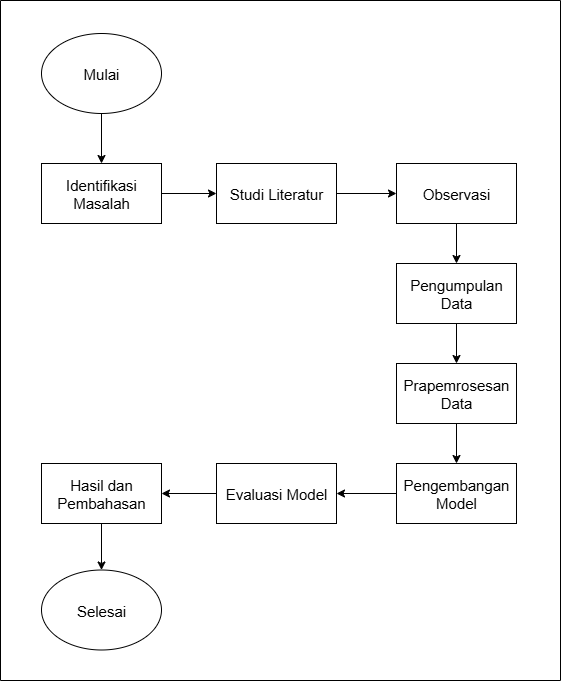
\includegraphics[width=0.9\textwidth]{figure/alurPenelitian.png}
    \caption{Alur Penelitian}
    \label{fig:3.alur}
\end{figure}

\section{Penjabaran Langkah Penelitian} \label{III.Jabar Alur}
Pada alur penelitian yang ditunjukkan pada Gambar \ref{fig:3.alur}, berikut merupakan penjabaran mengenai langkah penelitian yang dilakukan. \par

\subsection{Identifikasi Masalah} \label{III.LangkahIdentifikasiMasalah}
Pada tahap identifikasi masalah ditemukan bahwa proses identifikasi mineral kasiterit di Laboratorium Eksplorasi PT. Timah Tbk. masih dilakukan secara manual menggunakan metode \textit{Grain Counting Analysis} (GCA) dengan bantuan mikroskop binokuler. Metode ini membutuhkan ketelitian dan pengalaman tinggi dari analis, karena setiap butiran mineral harus diamati dan dihitung satu per satu secara visual. Pendekatan tersebut memiliki keterbatasan seperti memerlukan waktu yang lama, bersifat subjektif, serta rentan terhadap kesalahan pengamatan akibat kelelahan visual. Selain itu, keberadaan butiran mineral yang saling tumpang tindih (\textit{occluded}) juga menyebabkan kesulitan dalam membedakan batas antar butir kasiterit, sehingga dapat menurunkan akurasi hasil identifikasi. Oleh karena itu, penelitian ini berfokus untuk mengembangkan metode identifikasi mineral kasiterit menggunakan model \textit{Mask} R-CNN yang dapat melakukan segmentasi dengan menerapkan teknik \textit{amodal instance segmentation}, sehingga dapat digunakan untuk mengidentifikasi dan melakukan segmentasi bentuk utuh butir mineral kasiterit meskipun terjadi tumpang tindih antar butir pada citra mikroskop. \par

\subsection{Studi Literatur} \label{III.LangkahStudiLiteratur}
Pada tahap ini dilakukan pengumpulan berbagai macam informasi, referensi, konsep dasar, serta teori yang menjadi landasan dilakukannya penelitian ini. Proses ini dilakukan dengan mencari referensi berupa buku, jurnal, penelitian terdahulu, publikasi ilmiah, maupun sumber terpercaya lainnya yang berkaitan dengan penerapan \textit{deep learning} dalam bidang geologi, khususnya pada identifikasi mineral menggunakan citra mikroskop. Fokus kajian diarahkan pada pemahaman arsitektur \textit{Mask} R-CNN serta penerapan teknik \textit{amodal instance segmentation} yang digunakan untuk mengidentifikasi bentuk utuh butir mineral kasiterit meskipun terjadi tumpang tindih antar butir pada citra mikroskop. \par

\subsection{Observasi} \label{III.LangkahObservasi}
Kegiatan observasi dilakukan secara langsung di Laboratorium Eksplorasi PT. Timah Tbk. sebagai bagian dari proses pengumpulan data dan pemahaman terhadap sistem identifikasi mineral yang sedang diterapkan. Dalam kegiatan ini, peneliti melakukan kunjungan langsung ke laboratorium untuk melihat secara nyata proses identifikasi mineral menggunakan mikroskop yang menjadi bagian penting dari analisis mineralogi. Observasi dilakukan dengan tujuan untuk memahami kondisi aktual pelaksanaan analisis mineral di lapangan serta memperoleh gambaran awal mengenai metode yang digunakan dalam kegiatan laboratorium. \par

Selama kegiatan observasi, peneliti berkesempatan untuk melakukan wawancara langsung dengan Bapak Mesa Madestriasa selaku Kepala Laboratorium Eksplorasi PT. Timah Tbk. Wawancara ini bertujuan untuk memperoleh informasi terkait mekanisme identifikasi mineral kasiterit yang sedang diterapkan, permasalahan yang dihadapi selama proses analisis, serta faktor-faktor yang memengaruhi keakuratan hasil pengamatan mikroskopis. Dari hasil wawancara, diketahui bahwa kegiatan identifikasi mineral di laboratorium masih dilakukan secara manual dengan tingkat ketergantungan tinggi terhadap kemampuan dan ketelitian analis. Metode tersebut memerlukan waktu cukup lama dan rawan menghasilkan variasi hasil identifikasi antar pengamat akibat faktor kelelahan visual maupun subjektivitas pengamatan. Gambar \ref{fig:Wawancara} pada Lampiran \ref{lampiran:Wawancara} merupakan dokumentasi kegiatan wawancara yang dilakukan oleh peneliti bersama Kepala Laboratorium Eksplorasi PT. Timah Tbk. sebagai bagian dari proses pengumpulan data penelitian. \par

Selain melakukan wawancara, peneliti juga mendapatkan kesempatan untuk mencoba secara langsung penggunaan mikroskop binokuler yang digunakan dalam proses identifikasi mineral. Kegiatan ini didampingi oleh salah satu tim analis di Laboratorium Eksplorasi PT. Timah Tbk. Selama pengamatan, peneliti mempelajari karakteristik visual mineral kasiterit seperti bentuk, warna, kilap, dan reflektivitasnya, serta membandingkannya dengan mineral ikutan lain yang sering muncul bersamaan pada sampel. Pengalaman langsung ini memberikan pemahaman yang lebih konkret mengenai tantangan identifikasi butiran mineral, terutama ketika butiran tersebut saling menutupi atau mengalami oklusi sebagian. Lampiran \ref{lampiran:Observasi} merupakan kumpulan dokumentasi hasil observasi yang dilakukan peneliti di Laboratorium Eksplorasi PT. Timah Tbk., yang menampilkan proses identifikasi mineral serta kondisi lingkungan penelitian secara langsung. \par

Berdasarkan hasil wawancara dan pengamatan tersebut, dapat disimpulkan bahwa metode manual yang diterapkan di laboratorium memiliki keterbatasan dalam hal efisiensi dan objektivitas. Kondisi ini menjadi dasar kuat bagi peneliti untuk mengembangkan pendekatan otomatis berbasis teknologi \textit{deep learning} menggunakan model \textit{Mask Region-based Convolutional Neural Network} (\textit{Mask} R-CNN). Model ini dipilih karena mampu melakukan deteksi dan segmentasi setiap butir mineral kasiterit secara presisi, bahkan dengan menerapkan teknik \textit{amodal instance segmentation} untuk merekonstruksi bentuk utuh mineral yang sebagian tertutup oleh butir lainnya. \par

Setelah kegiatan wawancara dan observasi selesai dilakukan, peneliti mengurus proses administratif berupa pengajuan surat pengantar resmi sebagai bentuk permohonan izin penelitian kepada pihak laboratorium. Surat ini digunakan sebagai dasar legalitas untuk memperoleh data citra mikroskop yang akan digunakan dalam penelitian. Gambar \ref{fig:SuratIzinPenelitian} pada Lampiran \ref{lampiran:SuratIzin} merupakan hasil dari Surat Permohonan Izin Penelitian Tugas Akhir yang telah dibuat dan disetujui oleh pihak Fakultas Teknologi Industri, Institut Teknologi Sumatera sebagai dasar pelaksanaan kegiatan penelitian di PT. Timah Tbk.\par

\subsection{Pengumpulan Data} \label{III.LangkahPengumpulanData}
Data yang digunakan dalam penelitian ini berupa citra mikroskop mineral kasiterit yang merupakan data sekunder yang berasal dari Laboratorium Eksplorasi PT. Timah Tbk. Data tersebut diperoleh melalui Bapak Mesa Madestriasa selaku Kepala Laboratorium Eksplorasi PT. Timah Tbk. Gambar \ref{fig:PengumpulanData} pada Lampiran \ref{lampiran:Dataset} merupakan dokumentasi proses pengumpulan data yang dilakukan bersama Bapak Mesa Madestriasa. Proses ini dilakukan untuk memperoleh data pendukung penelitian berupa citra mikroskop yang telah dikumpulkan dan disimpan oleh pihak laboratorium. \par

Data yang didapatkan terdiri merupakan data citra mikroskop dengan berbagai mineral dan yang di gunakan sebanyak 142 citra mikroskop. % mencakup 7664 butir mineral kasiterit. 
Contoh citra pada dataset ditunjukkan pada Gambar \ref{fig:3.ContohDataset}. Gambar \ref{fig:PengantarPenelitian} pada Lampiran \ref{lampiran:SuratIzin} merupakan dokumentasi proses penyerahan surat izin penelitian oleh peneliti kepada Kepala Laboratorium Eksplorasi PT. Timah Tbk. sebagai bentuk permohonan resmi untuk pelaksanaan kegiatan penelitian di lingkungan laboratorium. \par

\begin{figure}[H] % Kalau menggunakan H, posisi gambar akan tepat dibawah teks
    \centering
    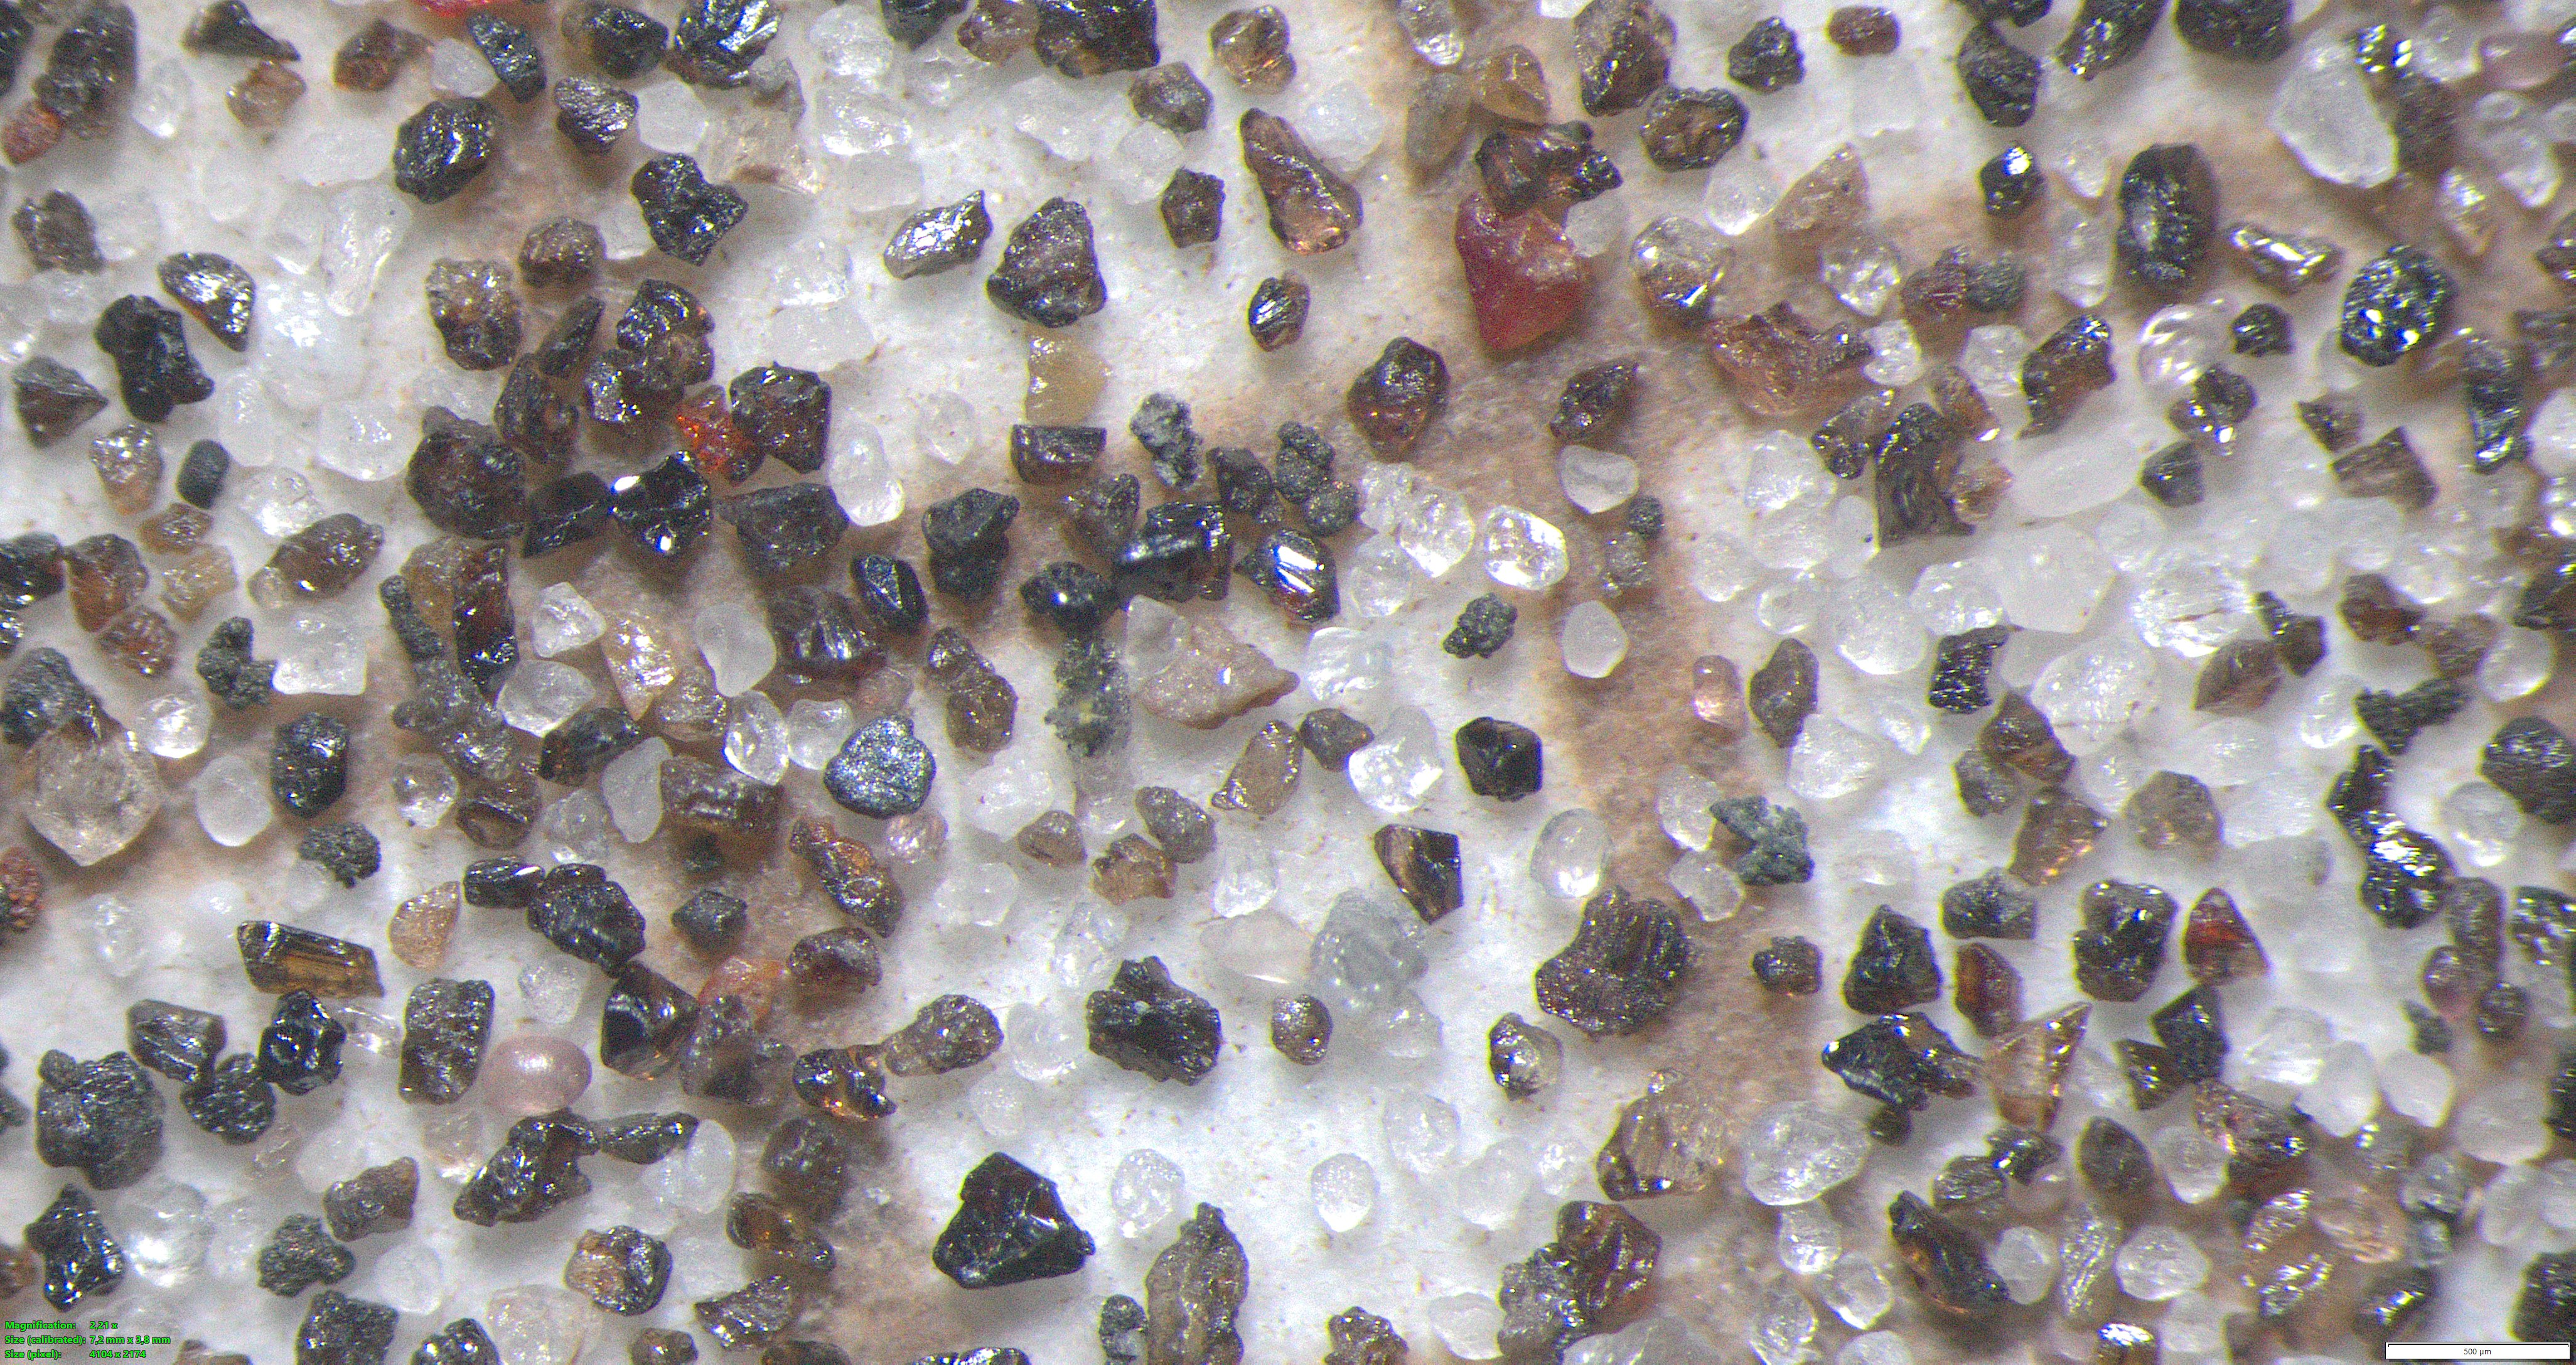
\includegraphics[width=1\textwidth]{figure/748-30100H.jpg}
    \caption{Contoh Gambar Dataset}
    \label{fig:3.ContohDataset}
\end{figure}

\subsection{Prapemrosesan Data} \label{III.LangkahPrapemrosesanData}
Pada penelitian ini, tahap prapemrosesan data dilakukan untuk mempersiapkan citra agar sesuai dengan kebutuhan model \textit{Mask} R-CNN. Tahap prapemrosesan meliputi pemilihan data untuk memastikan kualitas citra yang memadai, anotasi dan segmentasi data yang bertujuan untuk menandai serta memisahkan area objek kasiterit pada citra mikroskop, pembagian citra (\textit{image tiling}) yang digunakan untuk memecah citra menjadi beberapa bagian agar sesuai dengan kebutuhan input model, augmentasi data berupa \textit{flip} untuk membalik citra secara horizontal atau vertikal, \textit{rotate} untuk memutar citra pada sudut tertentu guna menambah variasi data, serta penambahan \textit{Gaussian noise} untuk meningkatkan ketahanan model terhadap gangguan visual, dan \textit{normalization} untuk menyesuaikan rentang nilai piksel citra agar berada dalam skala tertentu sehingga mempercepat konvergensi model. \par

\subsubsection{Pemilihan Data}
Dalam tahap prapemrosesan data, dilakukan proses pemilihan citra mikroskop untuk memastikan bahwa hanya citra dengan kualitas visual yang memadai yang digunakan dalam penelitian. Pemilihan ini mempertimbangkan beberapa faktor penting, termasuk tingkat pencahayaan serta kejelasan keberadaan objek mineral kasiterit pada citra mikroskop. Selain itu, citra yang tidak mengandung mineral kasiterit sebagai objek utama penelitian dikeluarkan dari proses selanjutnya. Citra dengan pencahayaan yang kurang memadai seperti pada Gambar \ref{fig:3.MilihGelap}, citra yang tidak menampilkan mineral kasiterit secara jelas seperti pada Gambar \ref{fig:3.MilihKurangJelas}, maupun citra yang tidak mengandung kasiterit seperti pada Gambar \ref{fig:3.MilihZircon}, dianggap tidak memenuhi kriteria kualitas data.

Berdasarkan proses seleksi tersebut, diperoleh sebanyak 142 citra mikroskop yang telah dinilai layak dan representatif oleh tim analis di Laboratorium Eksplorasi PT. Timah Tbk. untuk digunakan pada tahap pelatihan dan evaluasi model. Contoh citra yang memenuhi kriteria kelayakan ditunjukkan pada Gambar \ref{fig:3.MilihBagus}, sedangkan perbandingan tingkat keoptimalan kualitas citra secara keseluruhan dapat dilihat pada Gambar \ref{fig:3.MilihComparison}. Proses pemilihan ini bertujuan untuk memastikan bahwa data yang digunakan memiliki kualitas visual yang konsisten serta mencerminkan karakteristik objek penelitian secara akurat. Selain itu, proses kurasi ini dapat membatasi kemampuan model untuk beradaptasi terhadap citra dunia nyata yang memiliki kualitas pencahayaan atau kejernihan yang kurang ideal.

\begin{figure}[H]
    \centering
    % Baris pertama: dua gambar sejajar
    \begin{subfigure}[b]{0.475\textwidth}
        \centering
        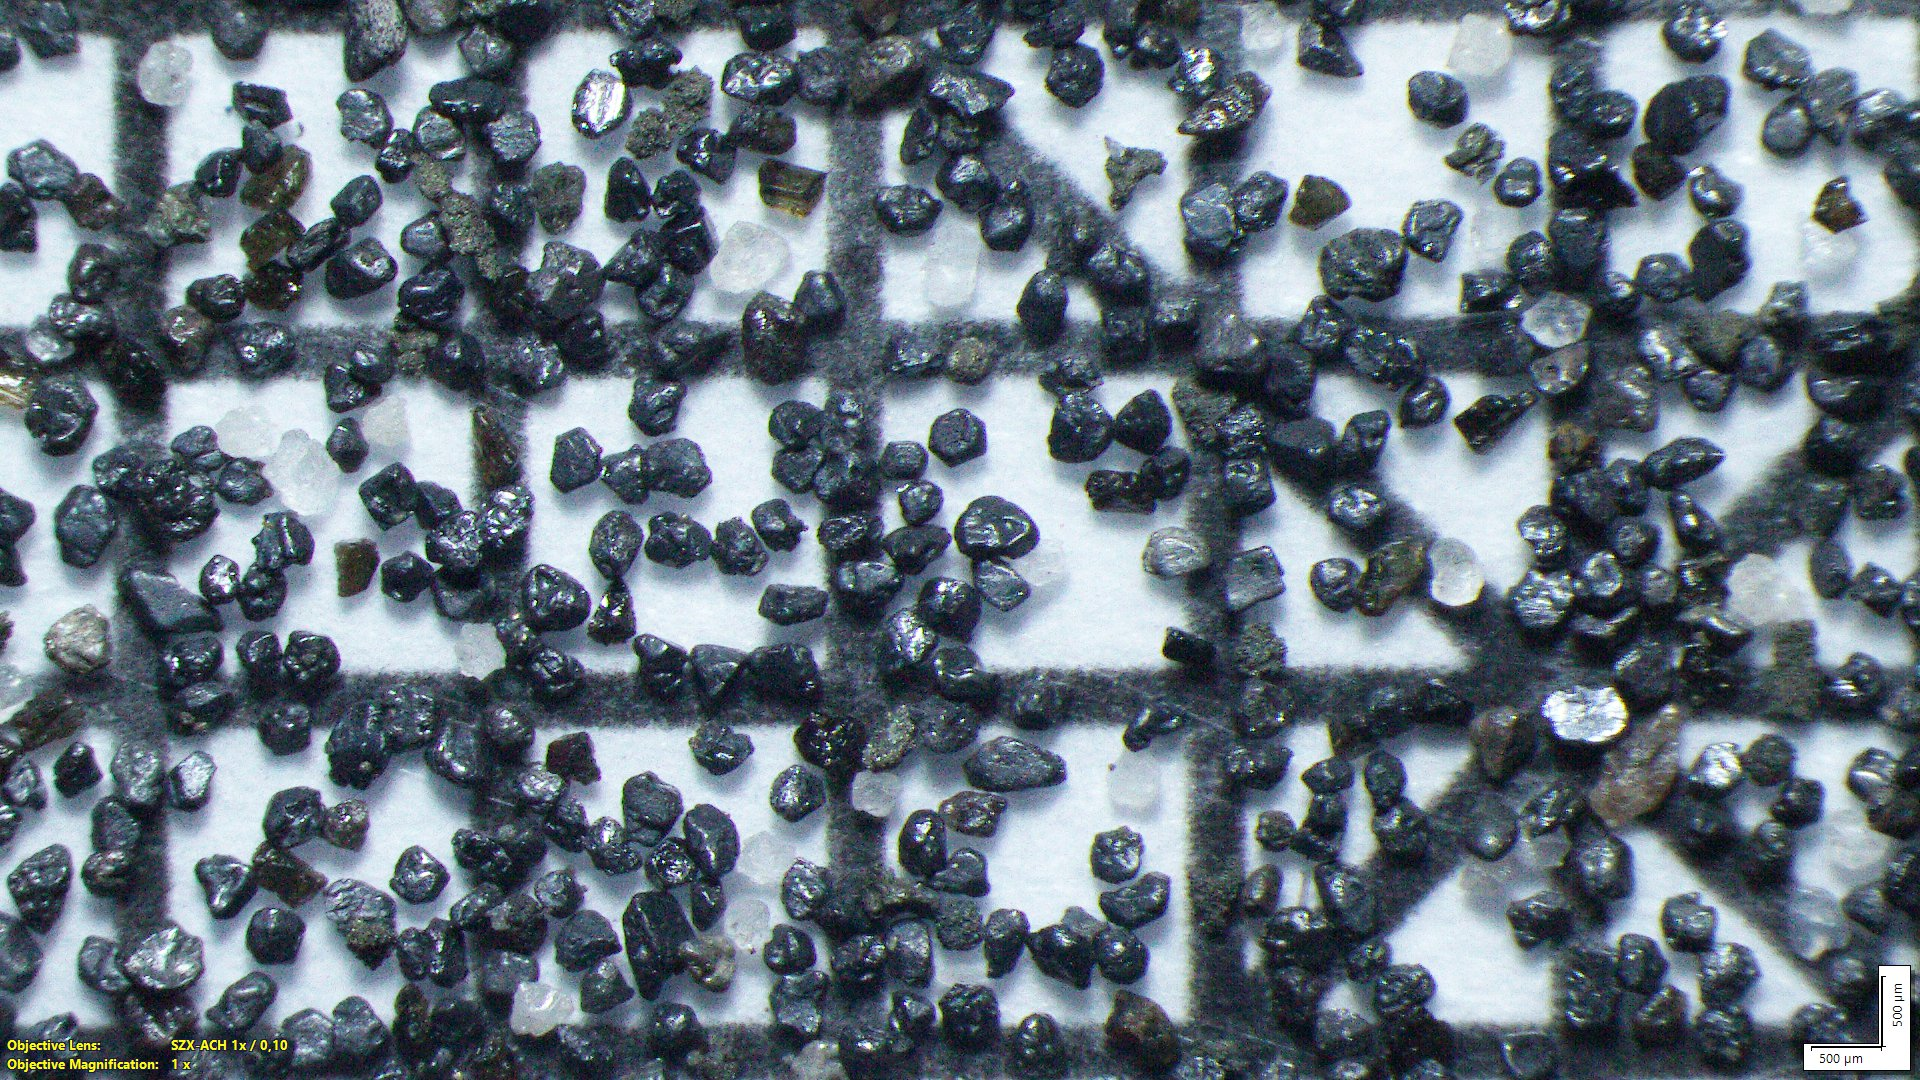
\includegraphics[width=\textwidth]{figure/MilihGelap.jpg}
        \caption{Citra dengan pencahayaan yang kurang memadai (Gelap)}
        \label{fig:3.MilihGelap}
    \end{subfigure}
    \hfill
    \begin{subfigure}[b]{0.475\textwidth}
        \centering
        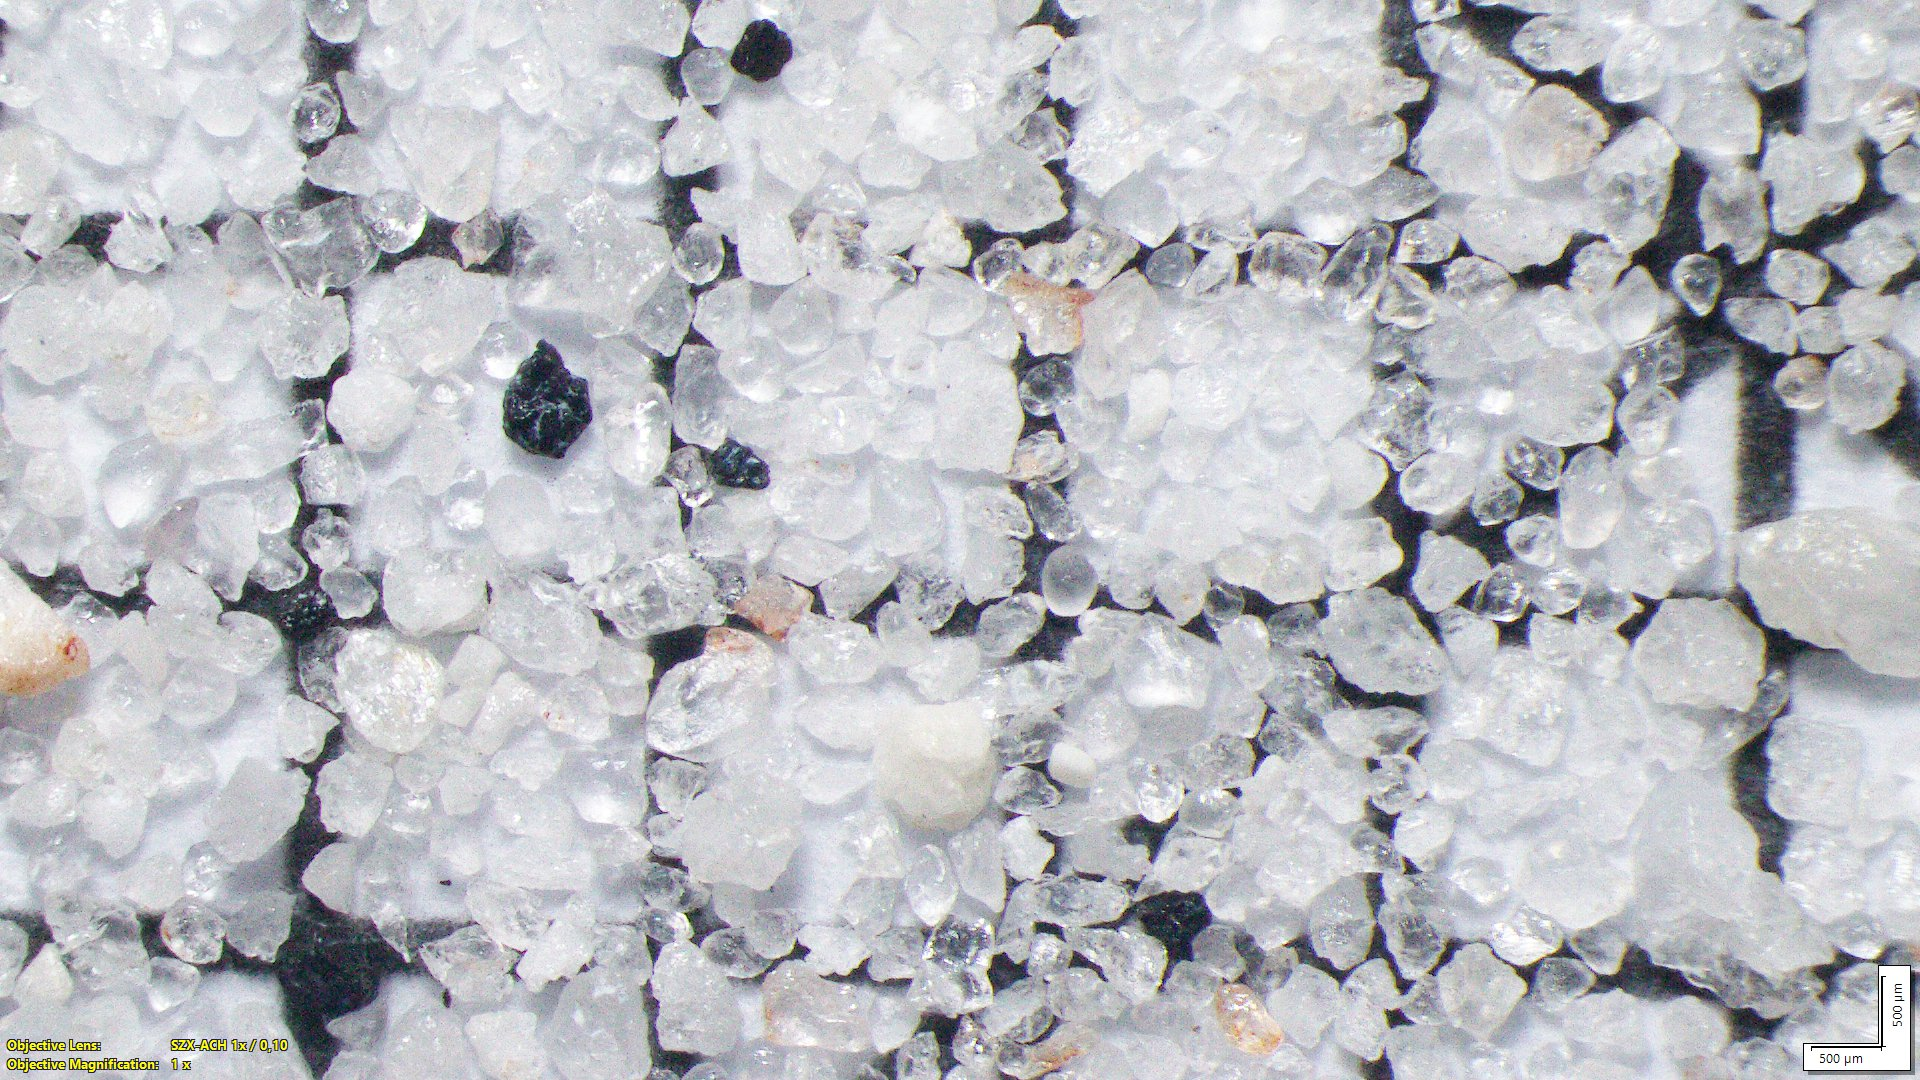
\includegraphics[width=\textwidth]{figure/MilihKurangJelas.jpg}
        \caption{Citra tidak menunjukkan keberadaan mineral target secara jelas}
        \label{fig:3.MilihKurangJelas}
    \end{subfigure}
    
    % Baris kedua: satu gambar di bawah tengah
    \vskip\baselineskip
    \begin{subfigure}[b]{0.475\textwidth}
        \centering
        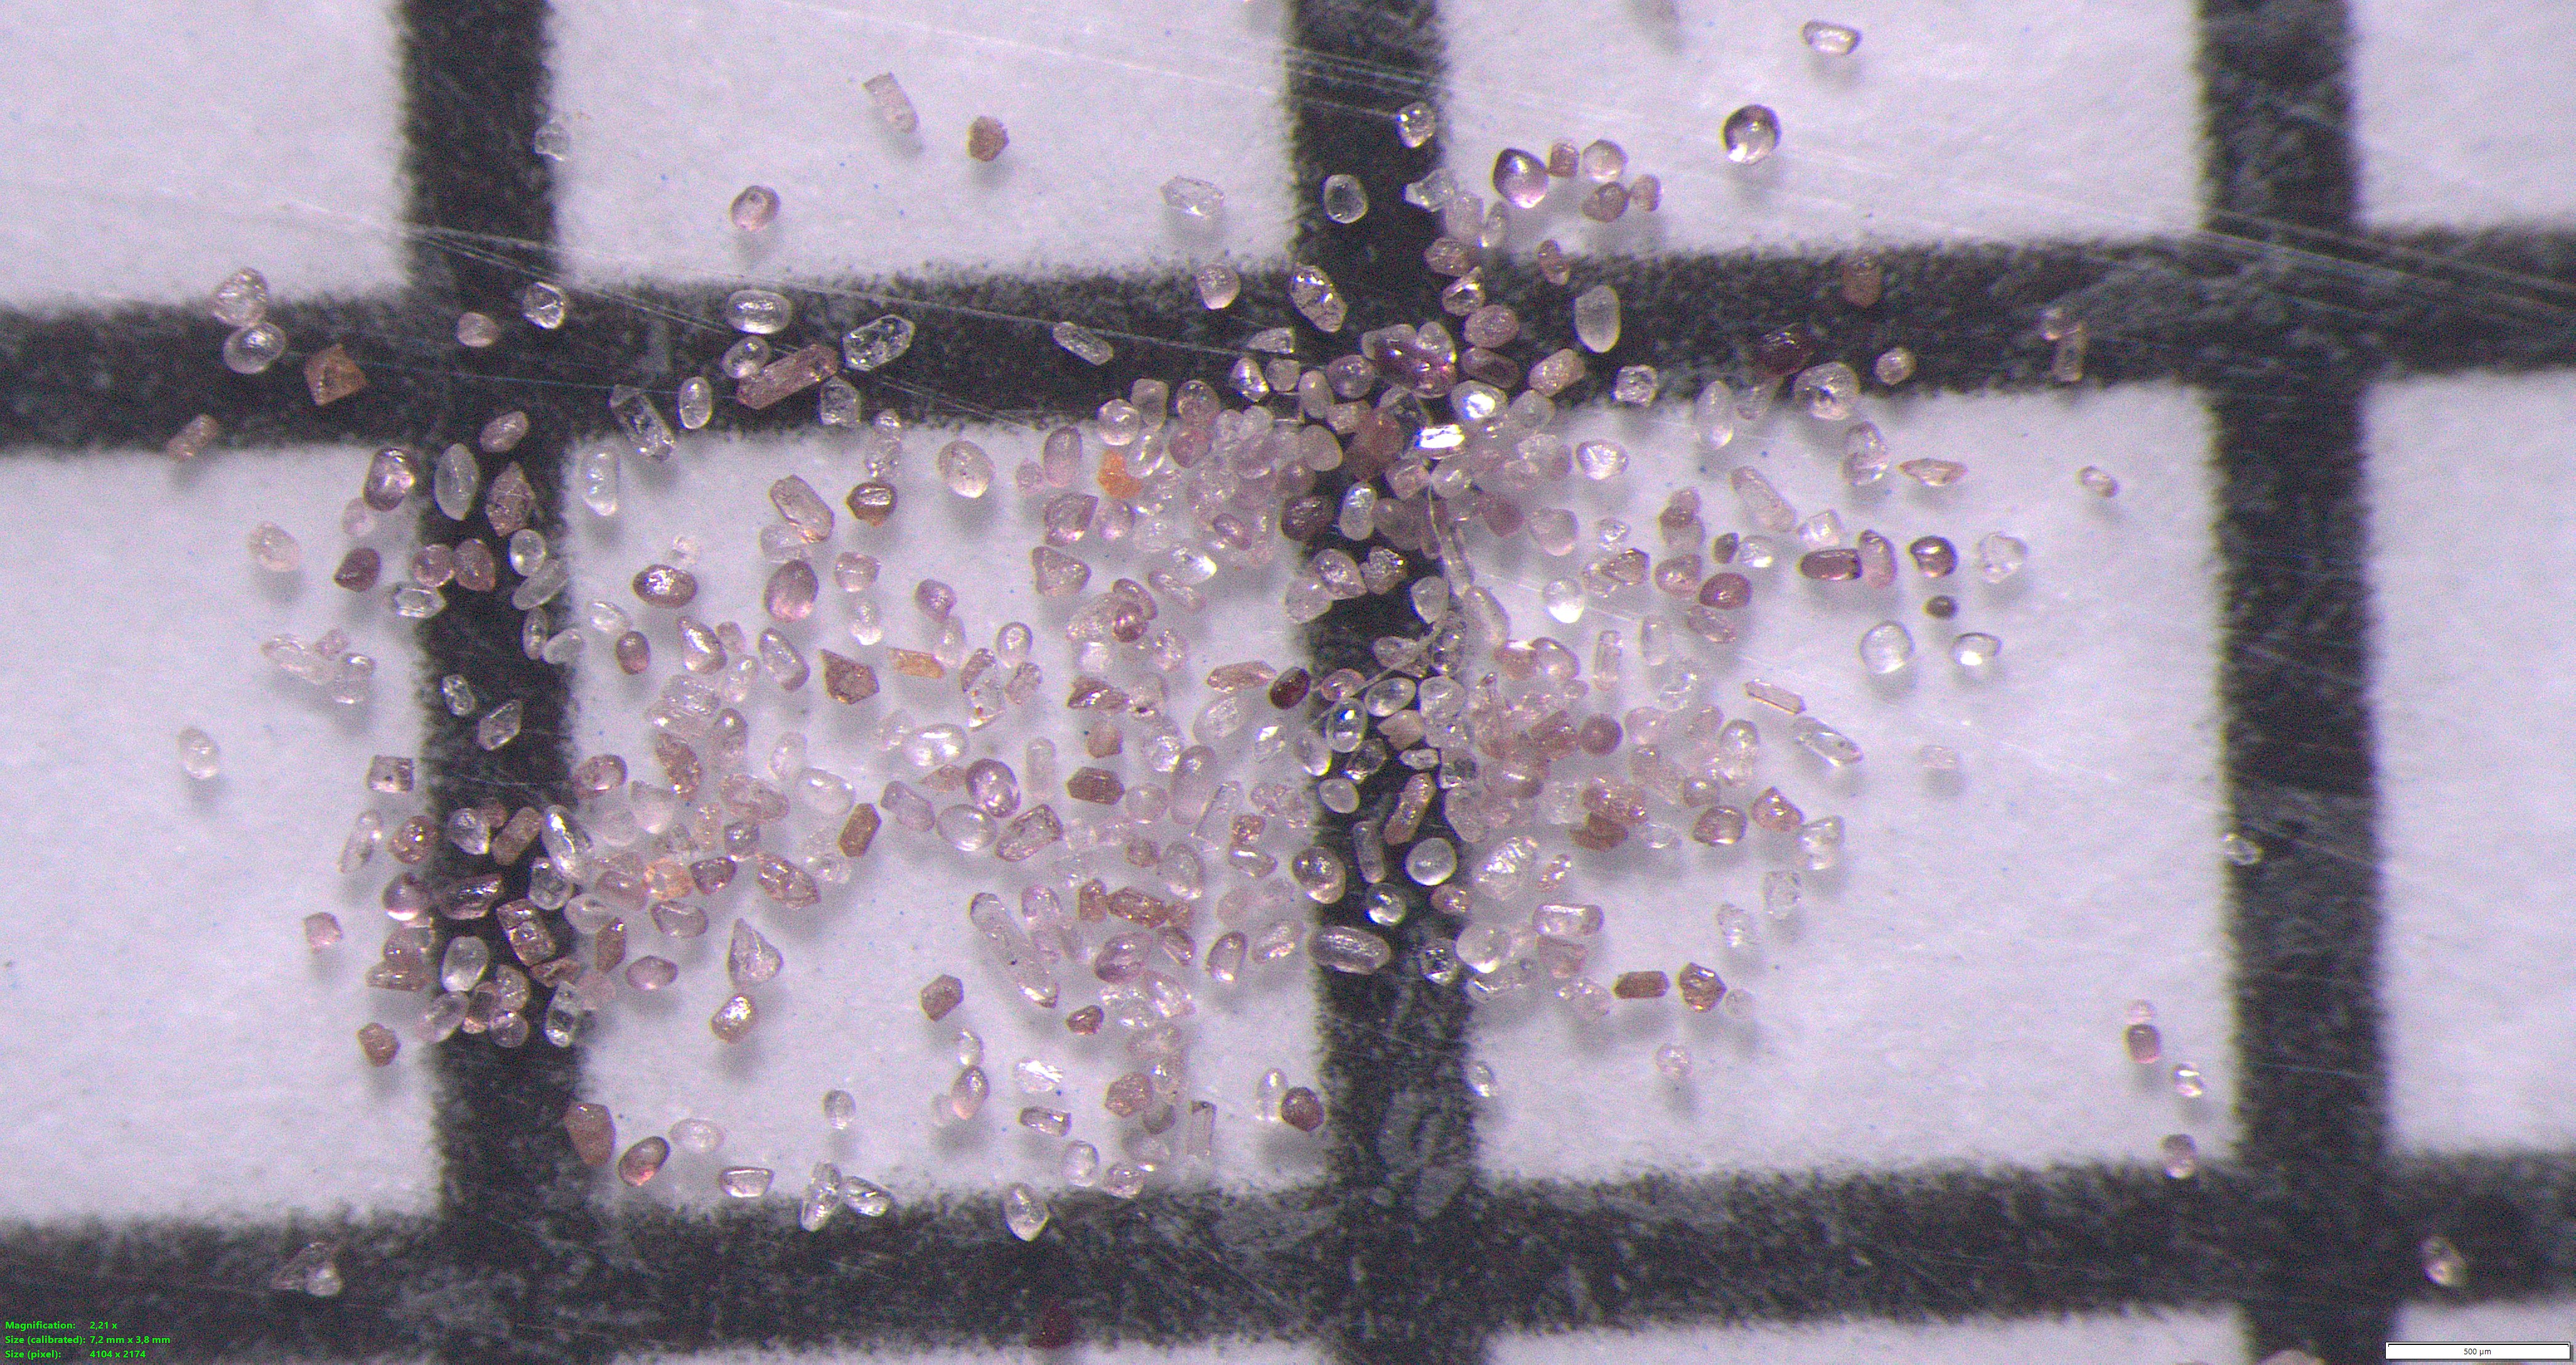
\includegraphics[width=\textwidth]{figure/MilihZircon.jpg}
        \caption{Citra yang tidak mengandung mineral kasiterit}
        \label{fig:3.MilihZircon}
    \end{subfigure}
    \hfill
    \begin{subfigure}[b]{0.475\textwidth}
        \centering
        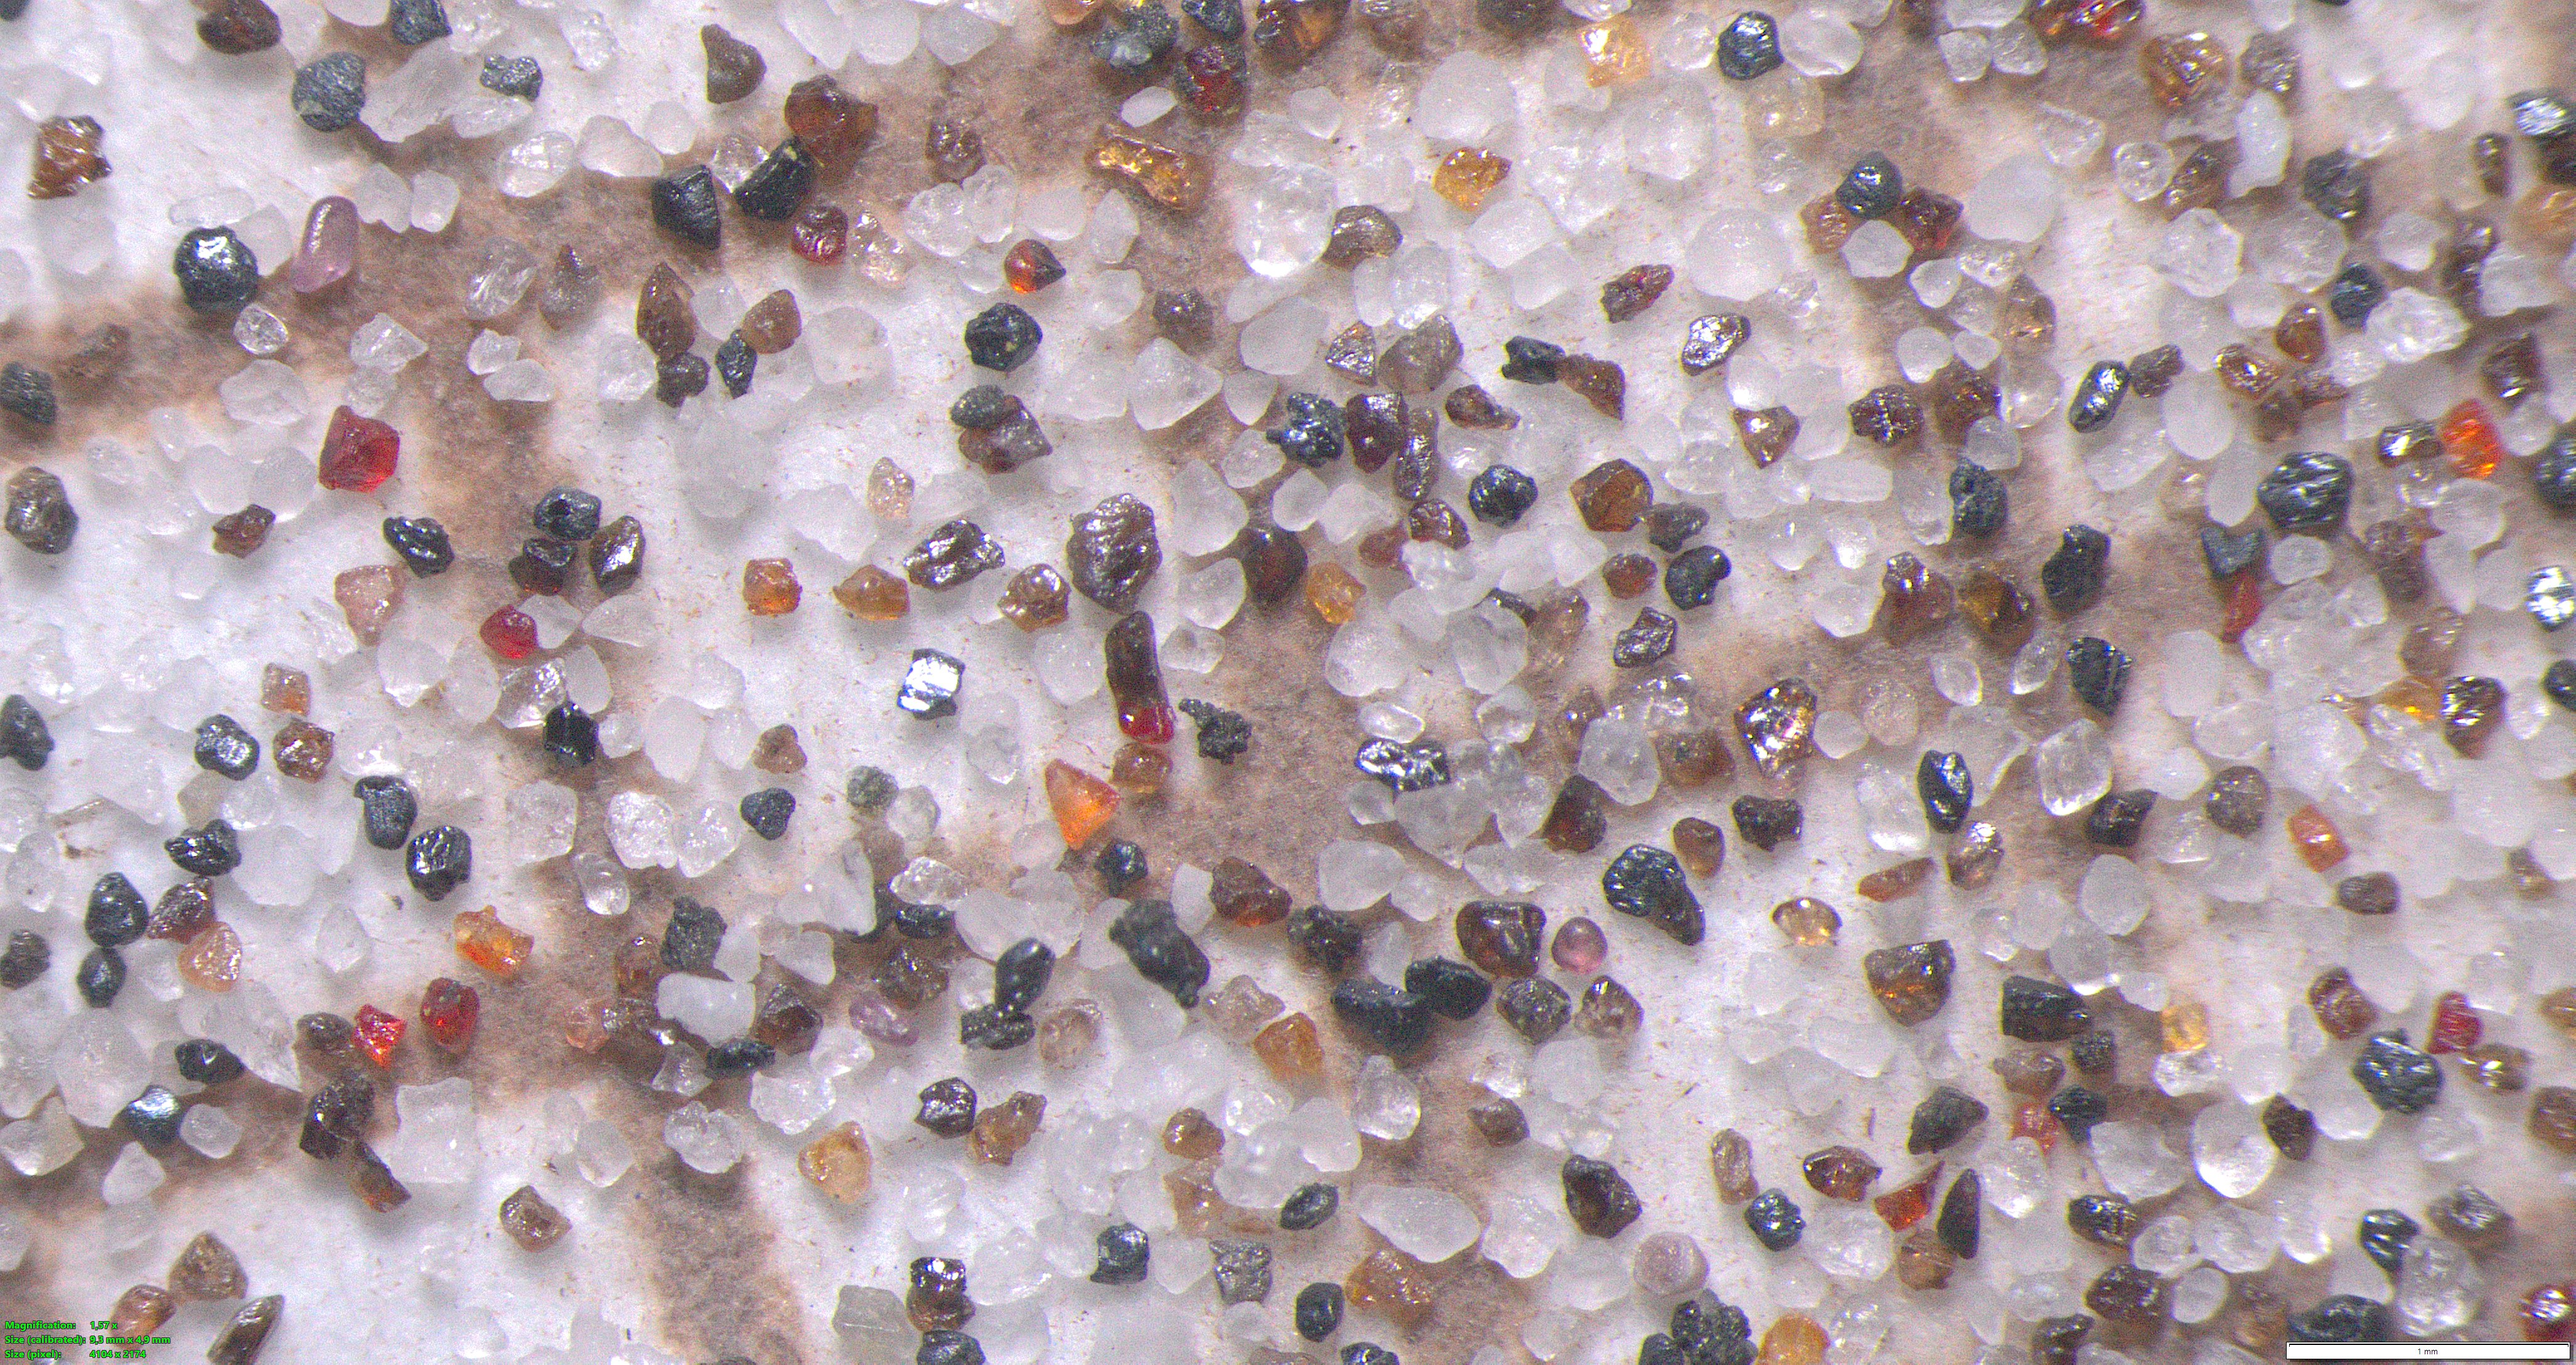
\includegraphics[width=\textwidth]{figure/MilihBagus.jpg}
        \caption{Citra pencahayaan dan kejelasannya optimal}
        \label{fig:3.MilihBagus}
    \end{subfigure}
    
    \caption{Perbandingan Tingkat Keoptimalan Data Citra Mikroskop}
    \label{fig:3.MilihComparison}
\end{figure}

\subsubsection{Anotasi Data}
Dalam proses anotasi data ini, peneliti terlebih dahulu melibatkan seorang anotator serta validator yang merupakan salah satu dari tim analis di Laboratorium Eksplorasi PT. Timah Tbk. untuk mengerjakan 10 citra mikroskop sebagai anotasi awal. Hasil dari anotasi tersebut kemudian dipelajari oleh peneliti untuk memahami pola dan standar anotasi yang telah ditetapkan. Setelah itu, peneliti melanjutkan proses anotasi secara mandiri terhadap 132 citra mikroskop tambahan. Seluruh hasil anotasi tersebut kemudian dievaluasi kembali oleh anotator yang sama guna memastikan konsistensi dan ketepatan anotasi. Proses evaluasi dilakukan dengan memberikan koreksi menggunakan warna berbeda, seperti warna merah untuk anotasi awal dan hijau untuk koreksi, sehingga perbedaan dapat teridentifikasi secara visual seperti yang terlihat pada Gambar \ref{fig:3.AnotasiAwal} dan Gambar \ref{fig:3.AnotasiEval}. Dokumentasi dari proses ini mencerminkan perbandingan antara hasil anotasi awal dengan hasil yang telah diperiksa, sekaligus menjadi bukti adanya proses revisi dan penyempurnaan. Contoh hasil anotasi data ditunjukkan pada Gambar \ref{fig:3.HasilAnotasiData} berikut.\par

\begin{figure}[H]
    \centering
    % Baris pertama: dua gambar sejajar
    \begin{subfigure}[b]{0.475\textwidth}
        \centering
        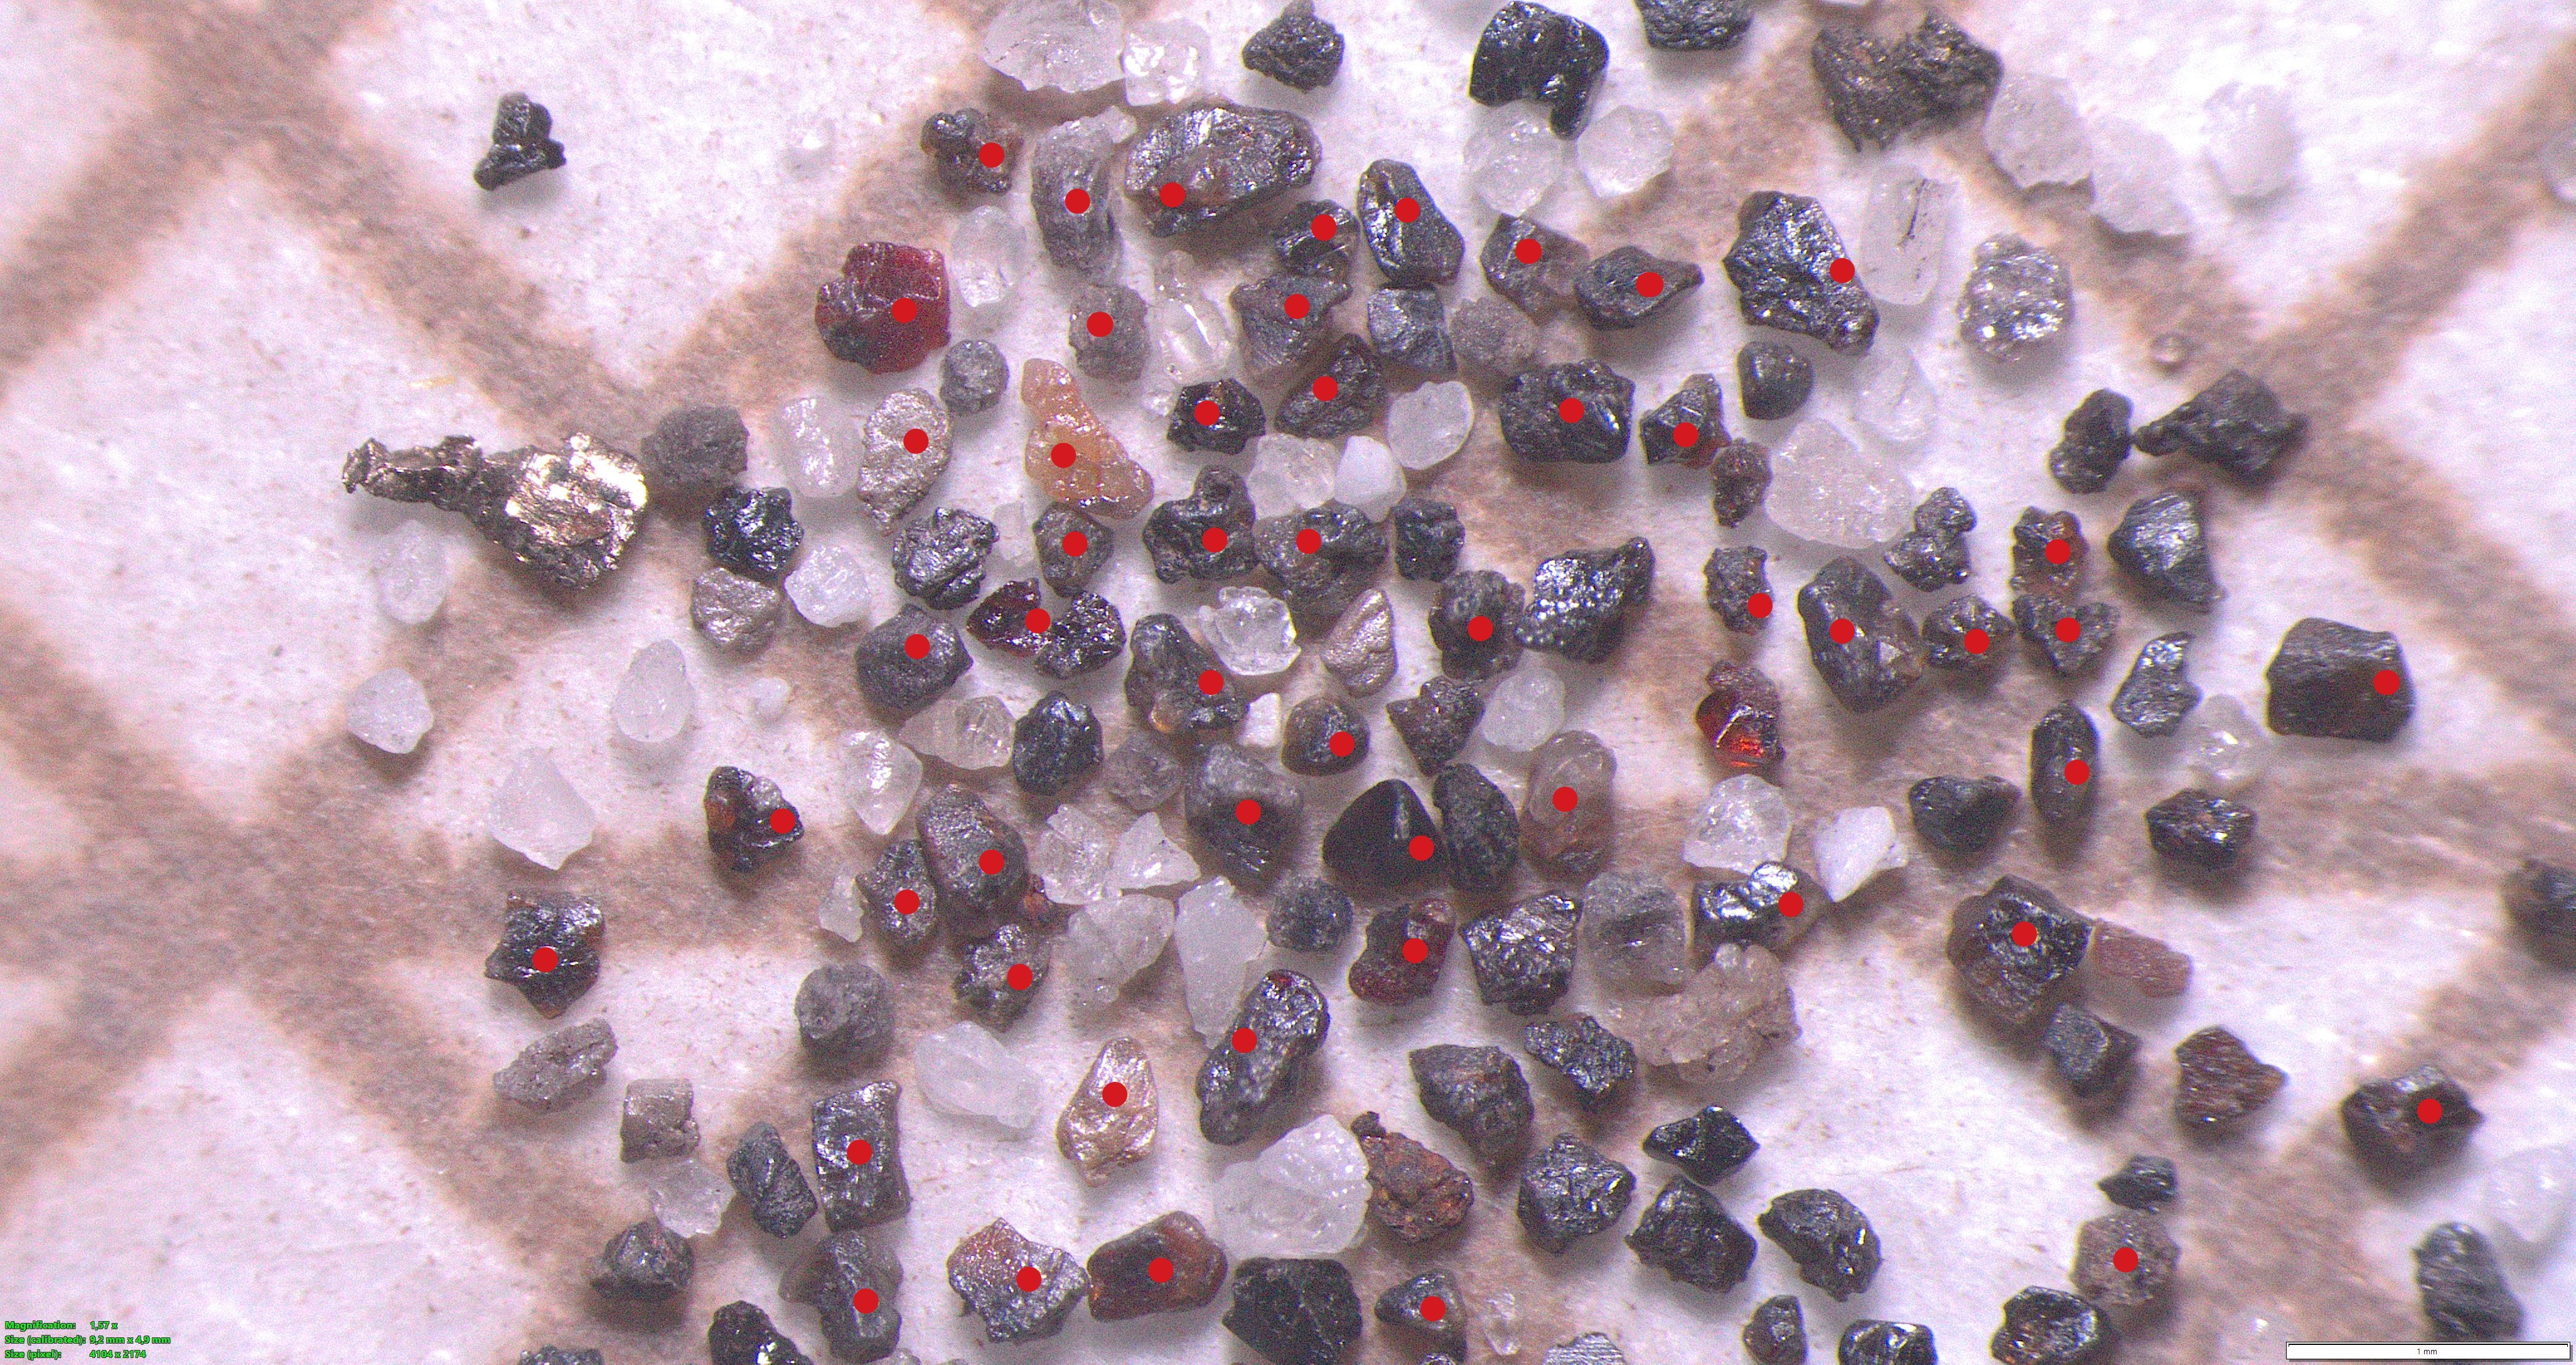
\includegraphics[width=\textwidth]{figure/anotasiAwal.jpg}
        \caption{Hasil Anotasi Awal yang di lakukan oleh \textit{Anotator}}
        \label{fig:3.AnotasiAwal}
    \end{subfigure}
    \hfill
    \begin{subfigure}[b]{0.475\textwidth}
        \centering
        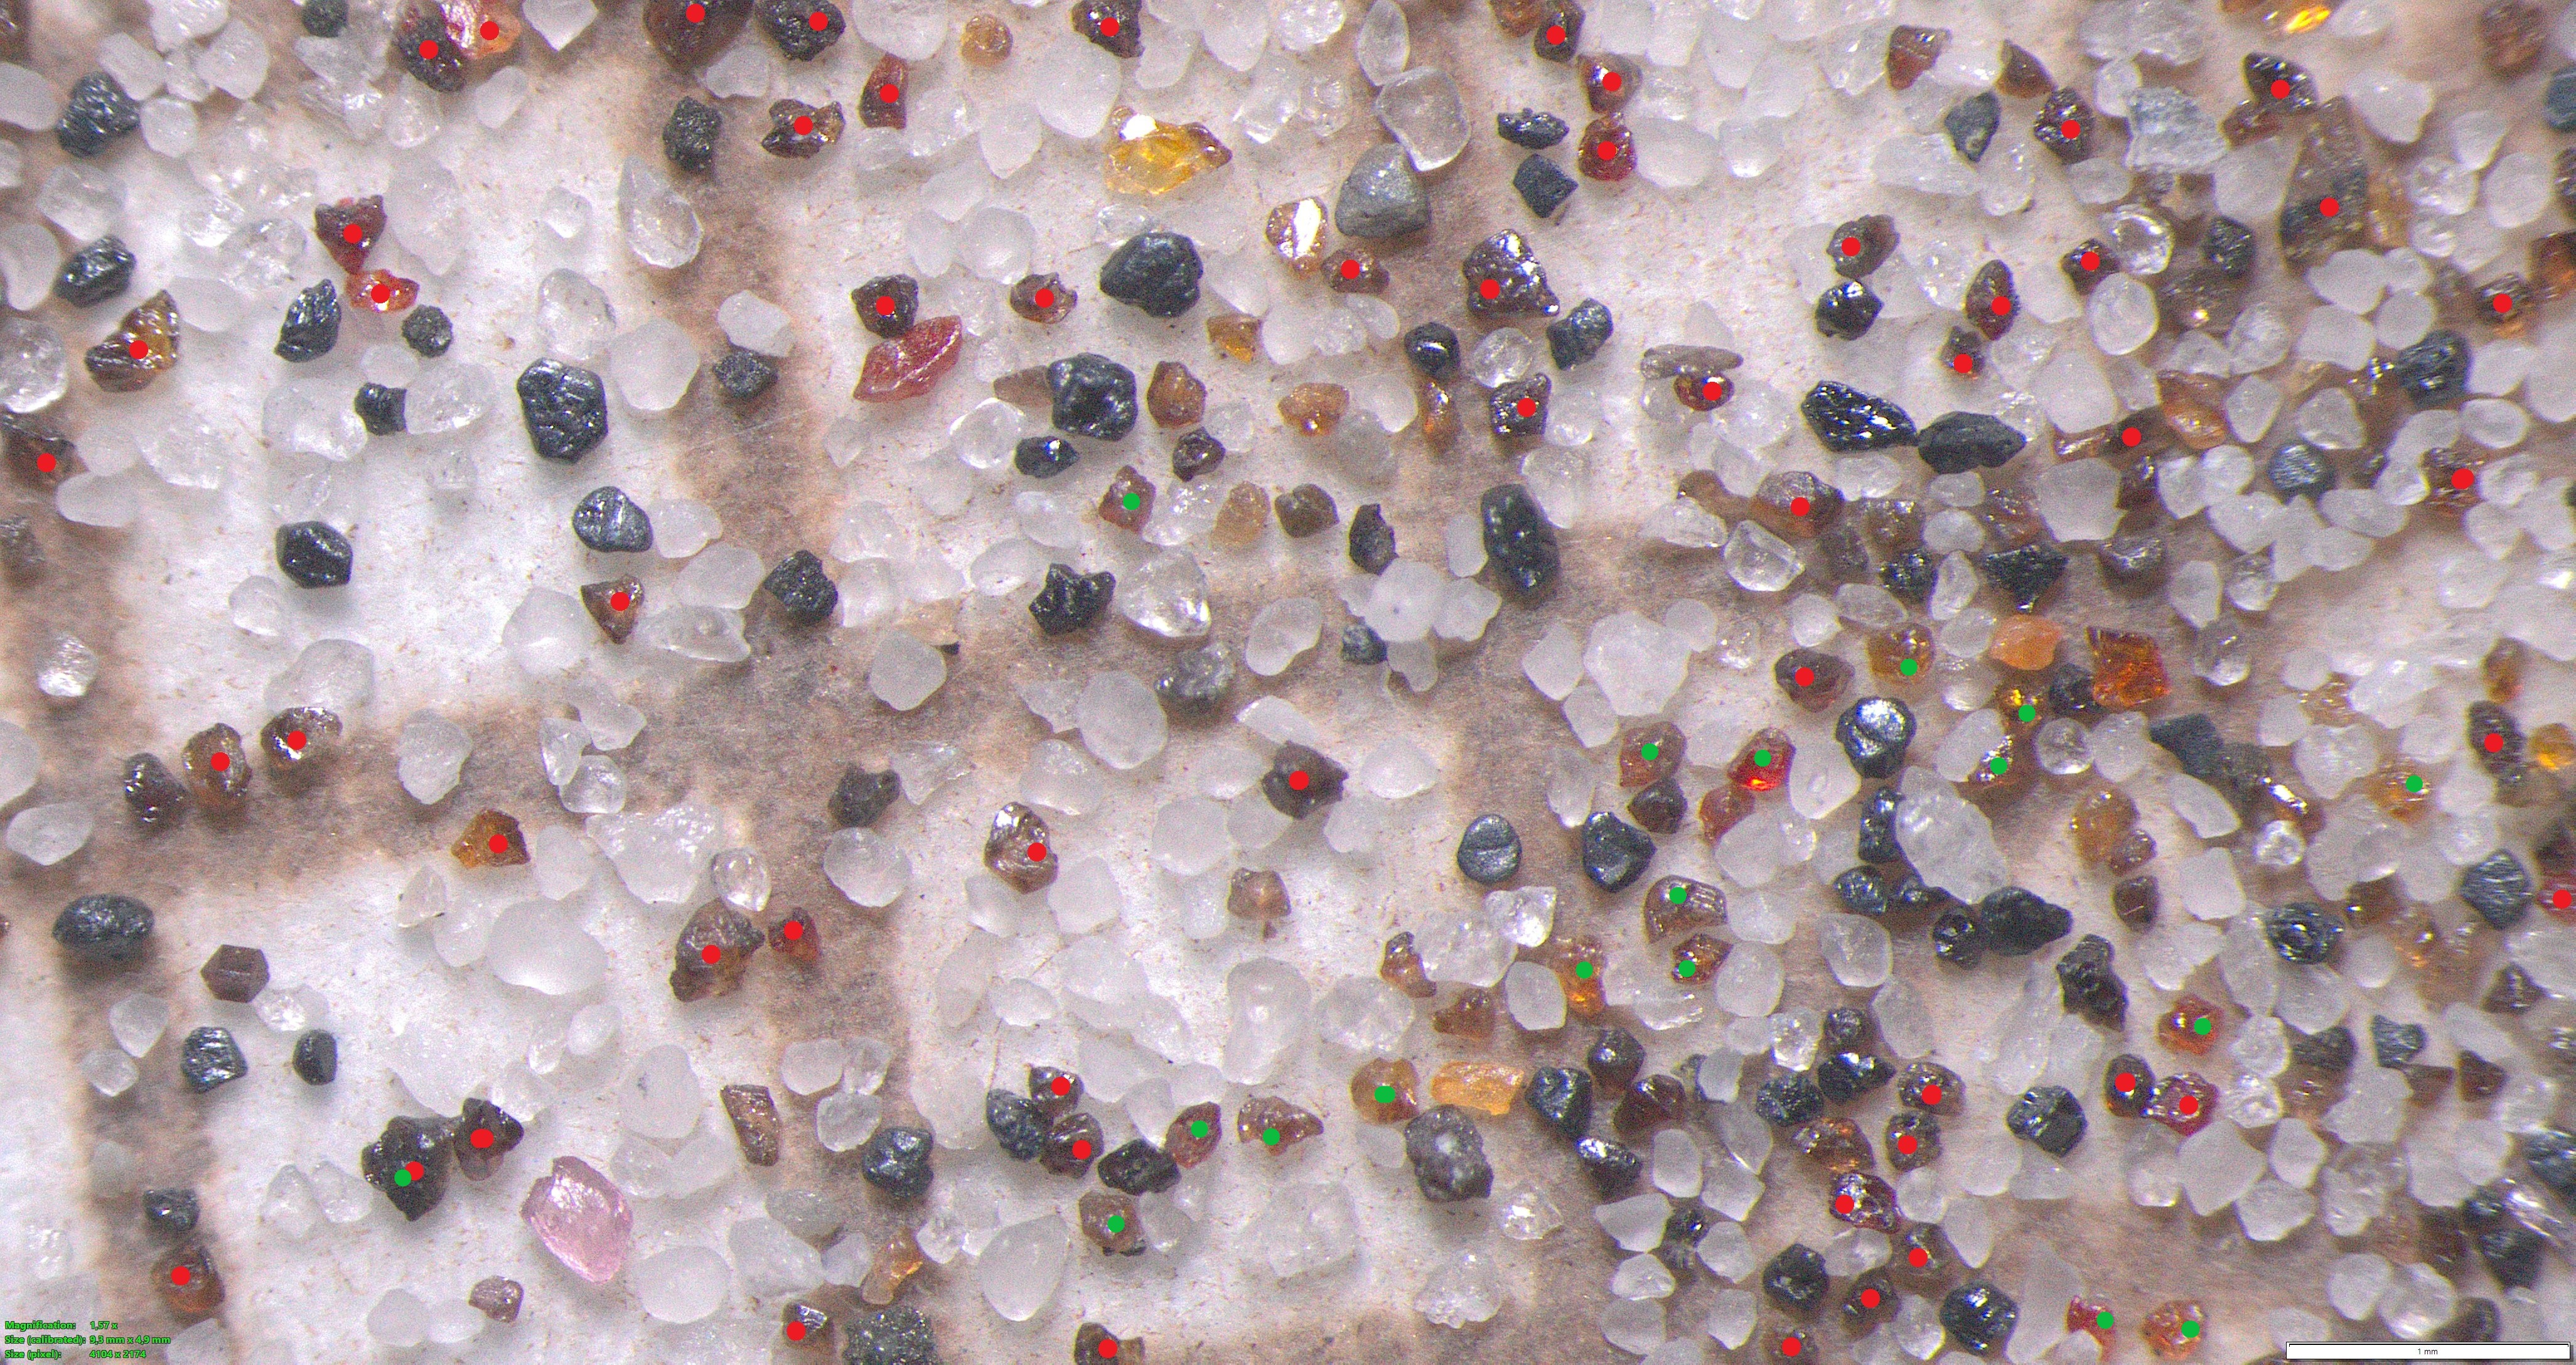
\includegraphics[width=\textwidth]{figure/AnotasiEval.jpg}
        \caption{Hasil Anotasi setelah di Evaluasi oleh \textit{Anotator}}
        \label{fig:3.AnotasiEval}
    \end{subfigure}

	\caption{Hasil Anotasi Data}
    \label{fig:3.HasilAnotasiData}
\end{figure}

\subsubsection{Segmentasi Data}
Pada tahap ini, dilakukan proses segmentasi data menggunakan LabelMe yang terintegrasi dengan \textit{Segment Anything} dengan fitur \textit{"Create Polygon with Segment Anything"}. Segmentasi dilakukan dengan metode poligon untuk mempermudah penandaan area kasiterit pada citra mikroskop. Dengan bantuan \textit{Segment Anything}, kontur mineral dapat diikuti secara otomatis, sehingga proses penandaan menjadi lebih efisien dan tetap fleksibel karena area mineral yang teroklusi dapat disesuaikan kembali secara manual dengan mengacu pada karakteristik bentuk kasiterit yang diperoleh dari wawancara pada tanggal 13 Agustus 2025 dengan Bapak Mesa Madestriasa selaku Kepala Laboratorium Eksplorasi PT. Timah Tbk., bahwa butiran kasiterit hasil preparasi umumnya berbentuk \textit{rounded} hingga \textit{sub-rounded} tanpa sudut angular, di mana tingkat kebulatanya semakin bulat pada butiran berukuran lebih kecil. Selain itu, penggunaan poligon yang dapat diedit membuat proses koreksi menjadi mudah dan tidak memerlukan langkah yang rumit. Labeling data dilakukan dalam satu kelas, setiap area yang ditandai diberi label yaitu \textit{"cassiterite"}. Dengan demikian, tahap ini memastikan bahwa data yang digunakan untuk pelatihan model segmentasi sudah teranotasi dan terlabel dengan baik. 

Dari keseluruhan proses segmentasi yang dilakukan terhadap 142 citra mikroskop, diperoleh total sebanyak 7,664 objek kasiterit yang berhasil diidentifikasi dan ditandai sebagai mask pada dataset. Jumlah ini merepresentasikan keseluruhan butiran kasiterit yang digunakan oleh model untuk mempelajari variasi bentuk, ukuran, serta karakteristik mineral pada tahap pelatihan. Contoh hasil segmentasi data ditunjukkan pada Gambar \ref{fig:3.HasilSegmentasiData} berikut. \par

\begin{figure}[H]
    \centering
    % Baris pertama: dua gambar sejajar
    \begin{subfigure}[b]{0.475\textwidth}
        \centering
        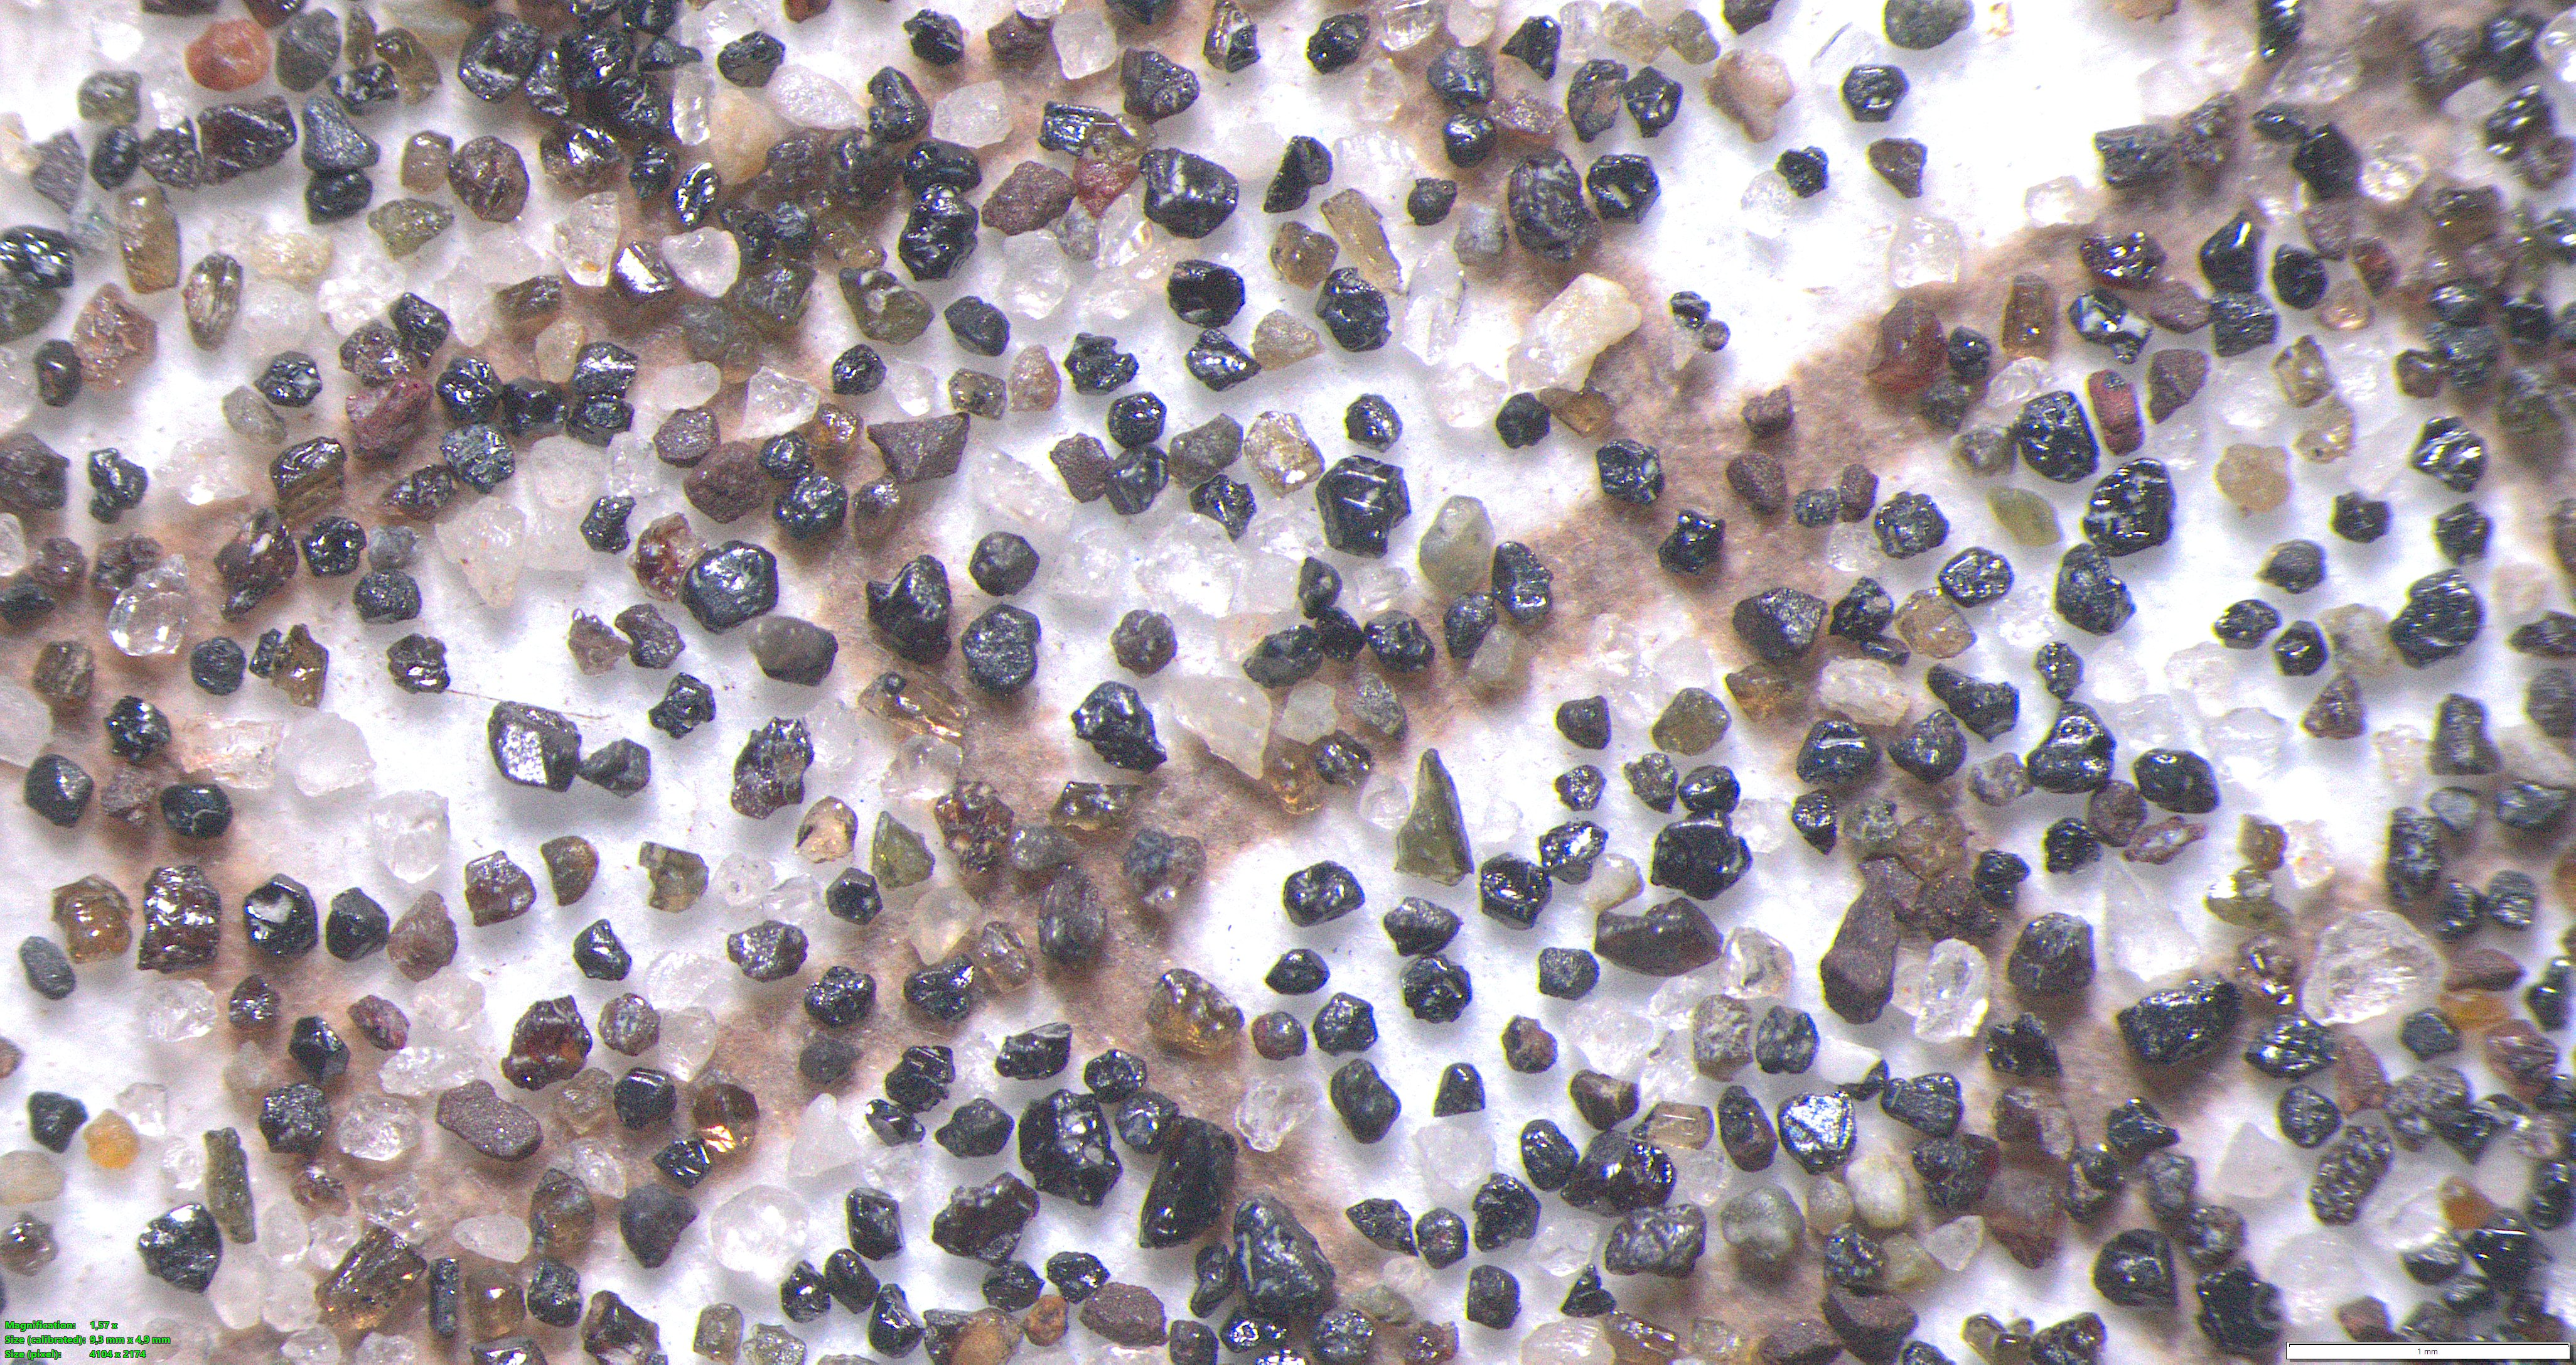
\includegraphics[width=\textwidth]{figure/input1.jpg}
        \caption{Data Sebelum Segmentasi}
        \label{fig:3.SebelumSegmentasi}
    \end{subfigure}
    \hfill
    \begin{subfigure}[b]{0.475\textwidth}
        \centering
        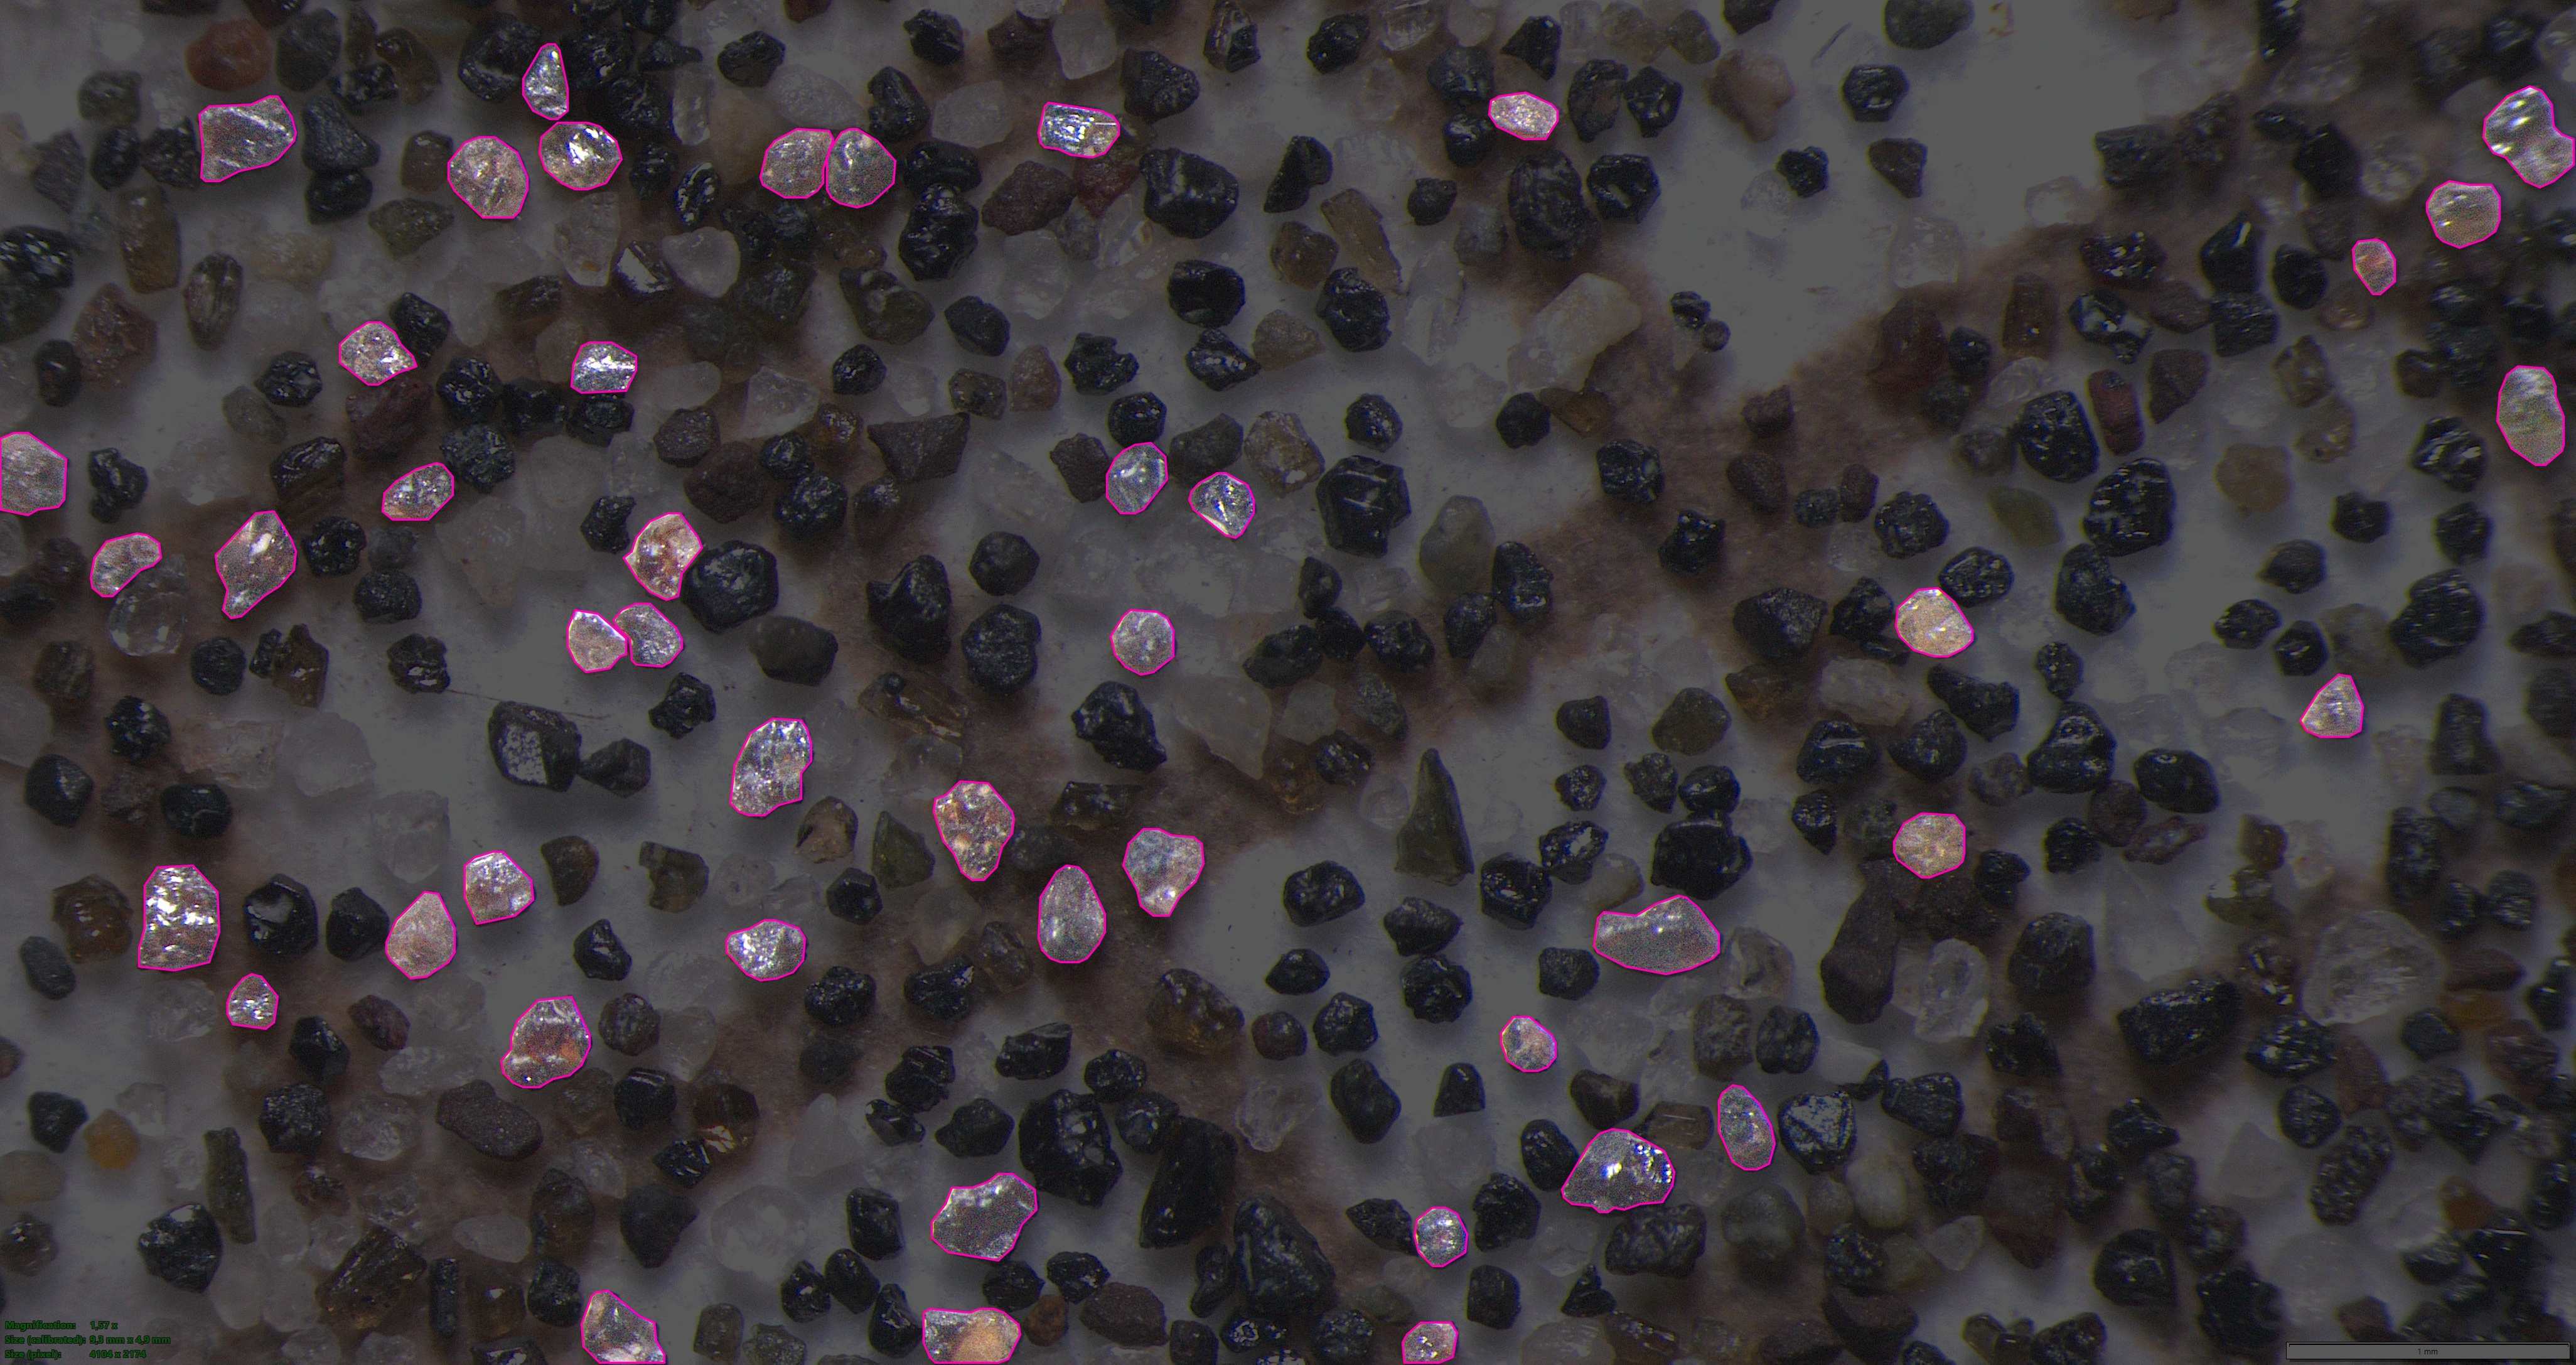
\includegraphics[width=\textwidth]{figure/output2.jpg}
        \caption{Data Setelah Segmentasi}
        \label{fig:3.SetelahSegmentasi}
    \end{subfigure}

	\caption{Hasil Segmentasi Data}
    \label{fig:3.HasilSegmentasiData}
\end{figure}

\subsubsection{Pembagian Citra (\textit{Image Tiling})} 
Pada tahap ini, dilakukan pembagian citra atau \textit{image tiling} untuk membagi citra beresolusi tinggi menjadi beberapa bagian yang lebih kecil atau \textit{patch}. Proses ini dilakukan sebagai alternatif dari proses \textit{resize} konvensional guna mempertahankan detail fitur pada butiran kasiterit yang berukuran kecil yang mungkin hilang jika resolusi citra dikurangi secara drastis. Dengan metode ini, model dapat mempelajari karakteristik objek pada resolusi aslinya tanpa melampaui kapasitas memori GPU. Citra asli dibagi menjadi grid $2 \times 2$, sehingga menghasilkan empat sub-citra yang lebih fokus. Contoh hasil pembagian citra ini ditunjukkan pada Gambar \ref{fig:3.HasilTilingData} berikut. \par

\begin{figure}[H]
    \centering
    % Baris pertama: satu gambar original di tengah
    \begin{subfigure}[b]{0.6\textwidth}
        \centering
        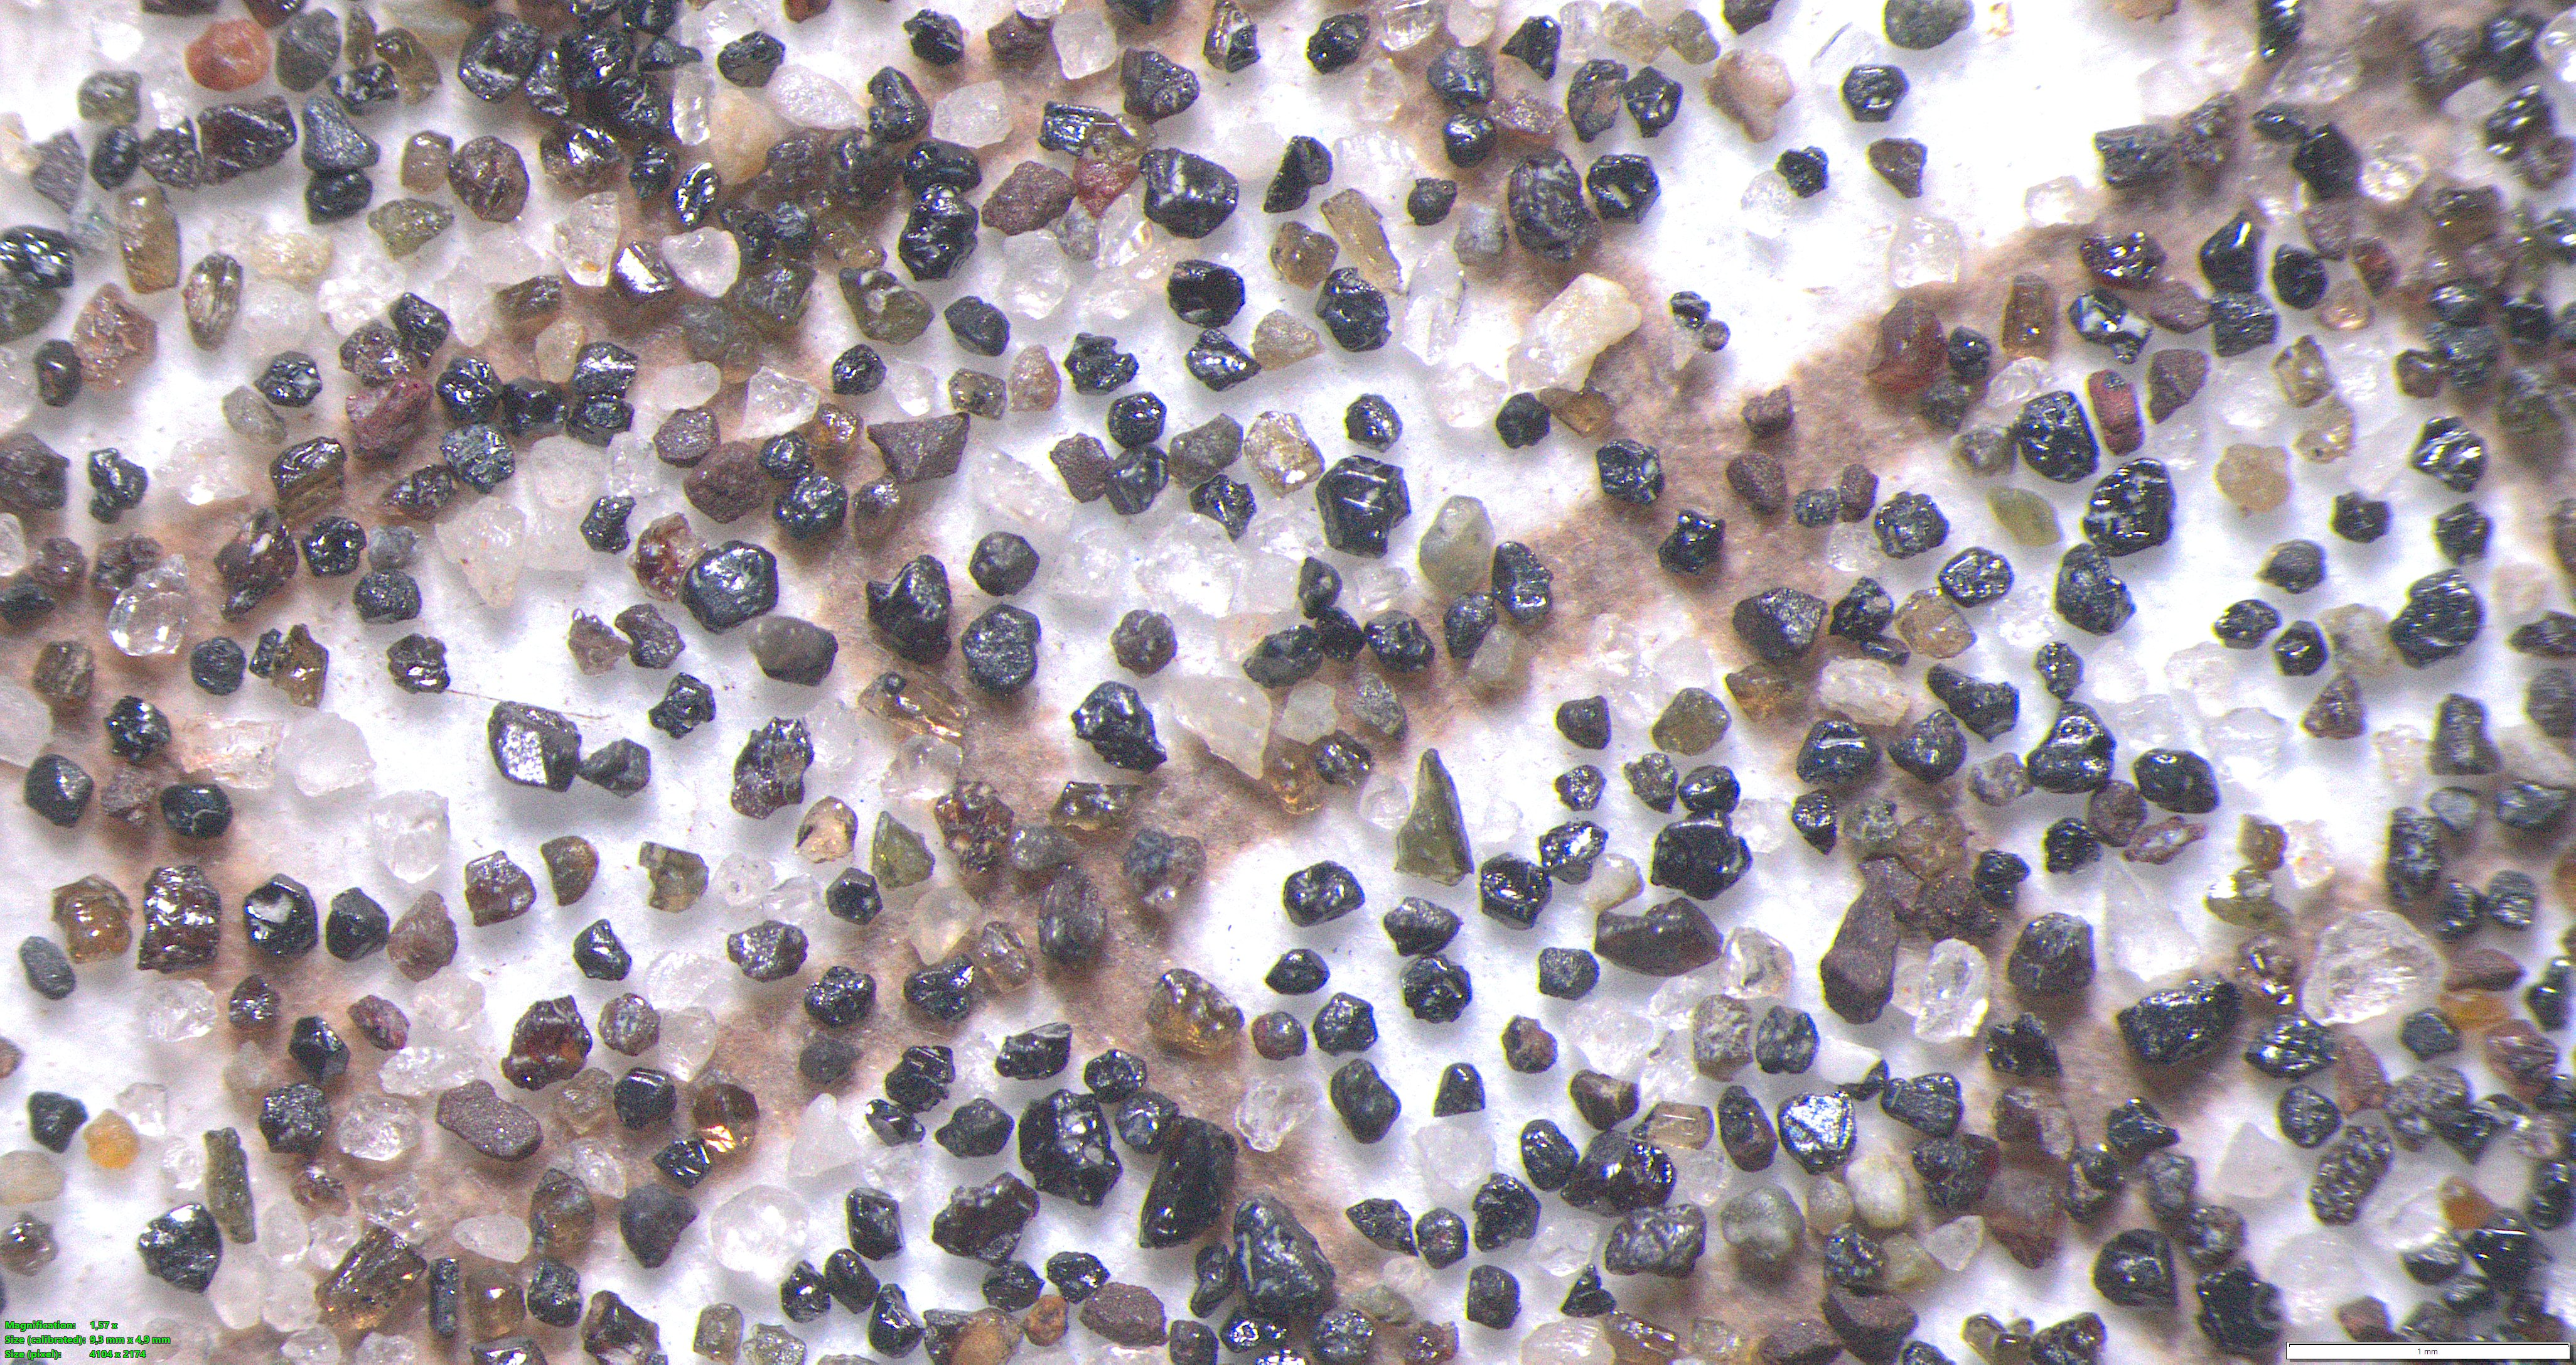
\includegraphics[width=\textwidth]{figure/tiles_285-25100F.jpg}
        \caption{Citra Original Sebelum \textit{Tiling}}
        \label{fig:3.TilingOriginal}
    \end{subfigure}
    
    \vskip\baselineskip
    
    % Baris kedua: grid 2x2 bagian atas
    \begin{subfigure}[b]{0.475\textwidth}
        \centering
        \includegraphics[width=\textwidth]{figure/285-25100F_tile0.png}
        \caption{Hasil \textit{Tiling} Bagian 1}
        \label{fig:3.Tile1}
    \end{subfigure}
    \hfill
    \begin{subfigure}[b]{0.475\textwidth}
        \centering
        \includegraphics[width=\textwidth]{figure/285-25100F_tile1.png}
        \caption{Hasil \textit{Tiling} Bagian 2}
        \label{fig:3.Tile2}
    \end{subfigure}
    
    \vskip\baselineskip
    
    % Baris ketiga: grid 2x2 bagian bawah
    \begin{subfigure}[b]{0.475\textwidth}
        \centering
        \includegraphics[width=\textwidth]{figure/285-25100F_tile2.png}
        \caption{Hasil \textit{Tiling} Bagian 3}
        \label{fig:3.Tile3}
    \end{subfigure}
    \hfill
    \begin{subfigure}[b]{0.475\textwidth}
        \centering
        \includegraphics[width=\textwidth]{figure/285-25100F_tile3.png}
        \caption{Hasil \textit{Tiling} Bagian 4}
        \label{fig:3.Tile4}
    \end{subfigure}

    \caption{Proses Pembagian Citra (\textit{Image Tiling}) Menjadi Grid $2 \times 2$}
    \label{fig:3.HasilTilingData}
\end{figure}

% % ini di bagi jadi 4 gambar
% \begin{figure}[H]
%     \centering
    
%     % Gambar original (tetap di atas, tengah)
%     \begin{subfigure}[b]{0.6\textwidth}
%         \centering
%         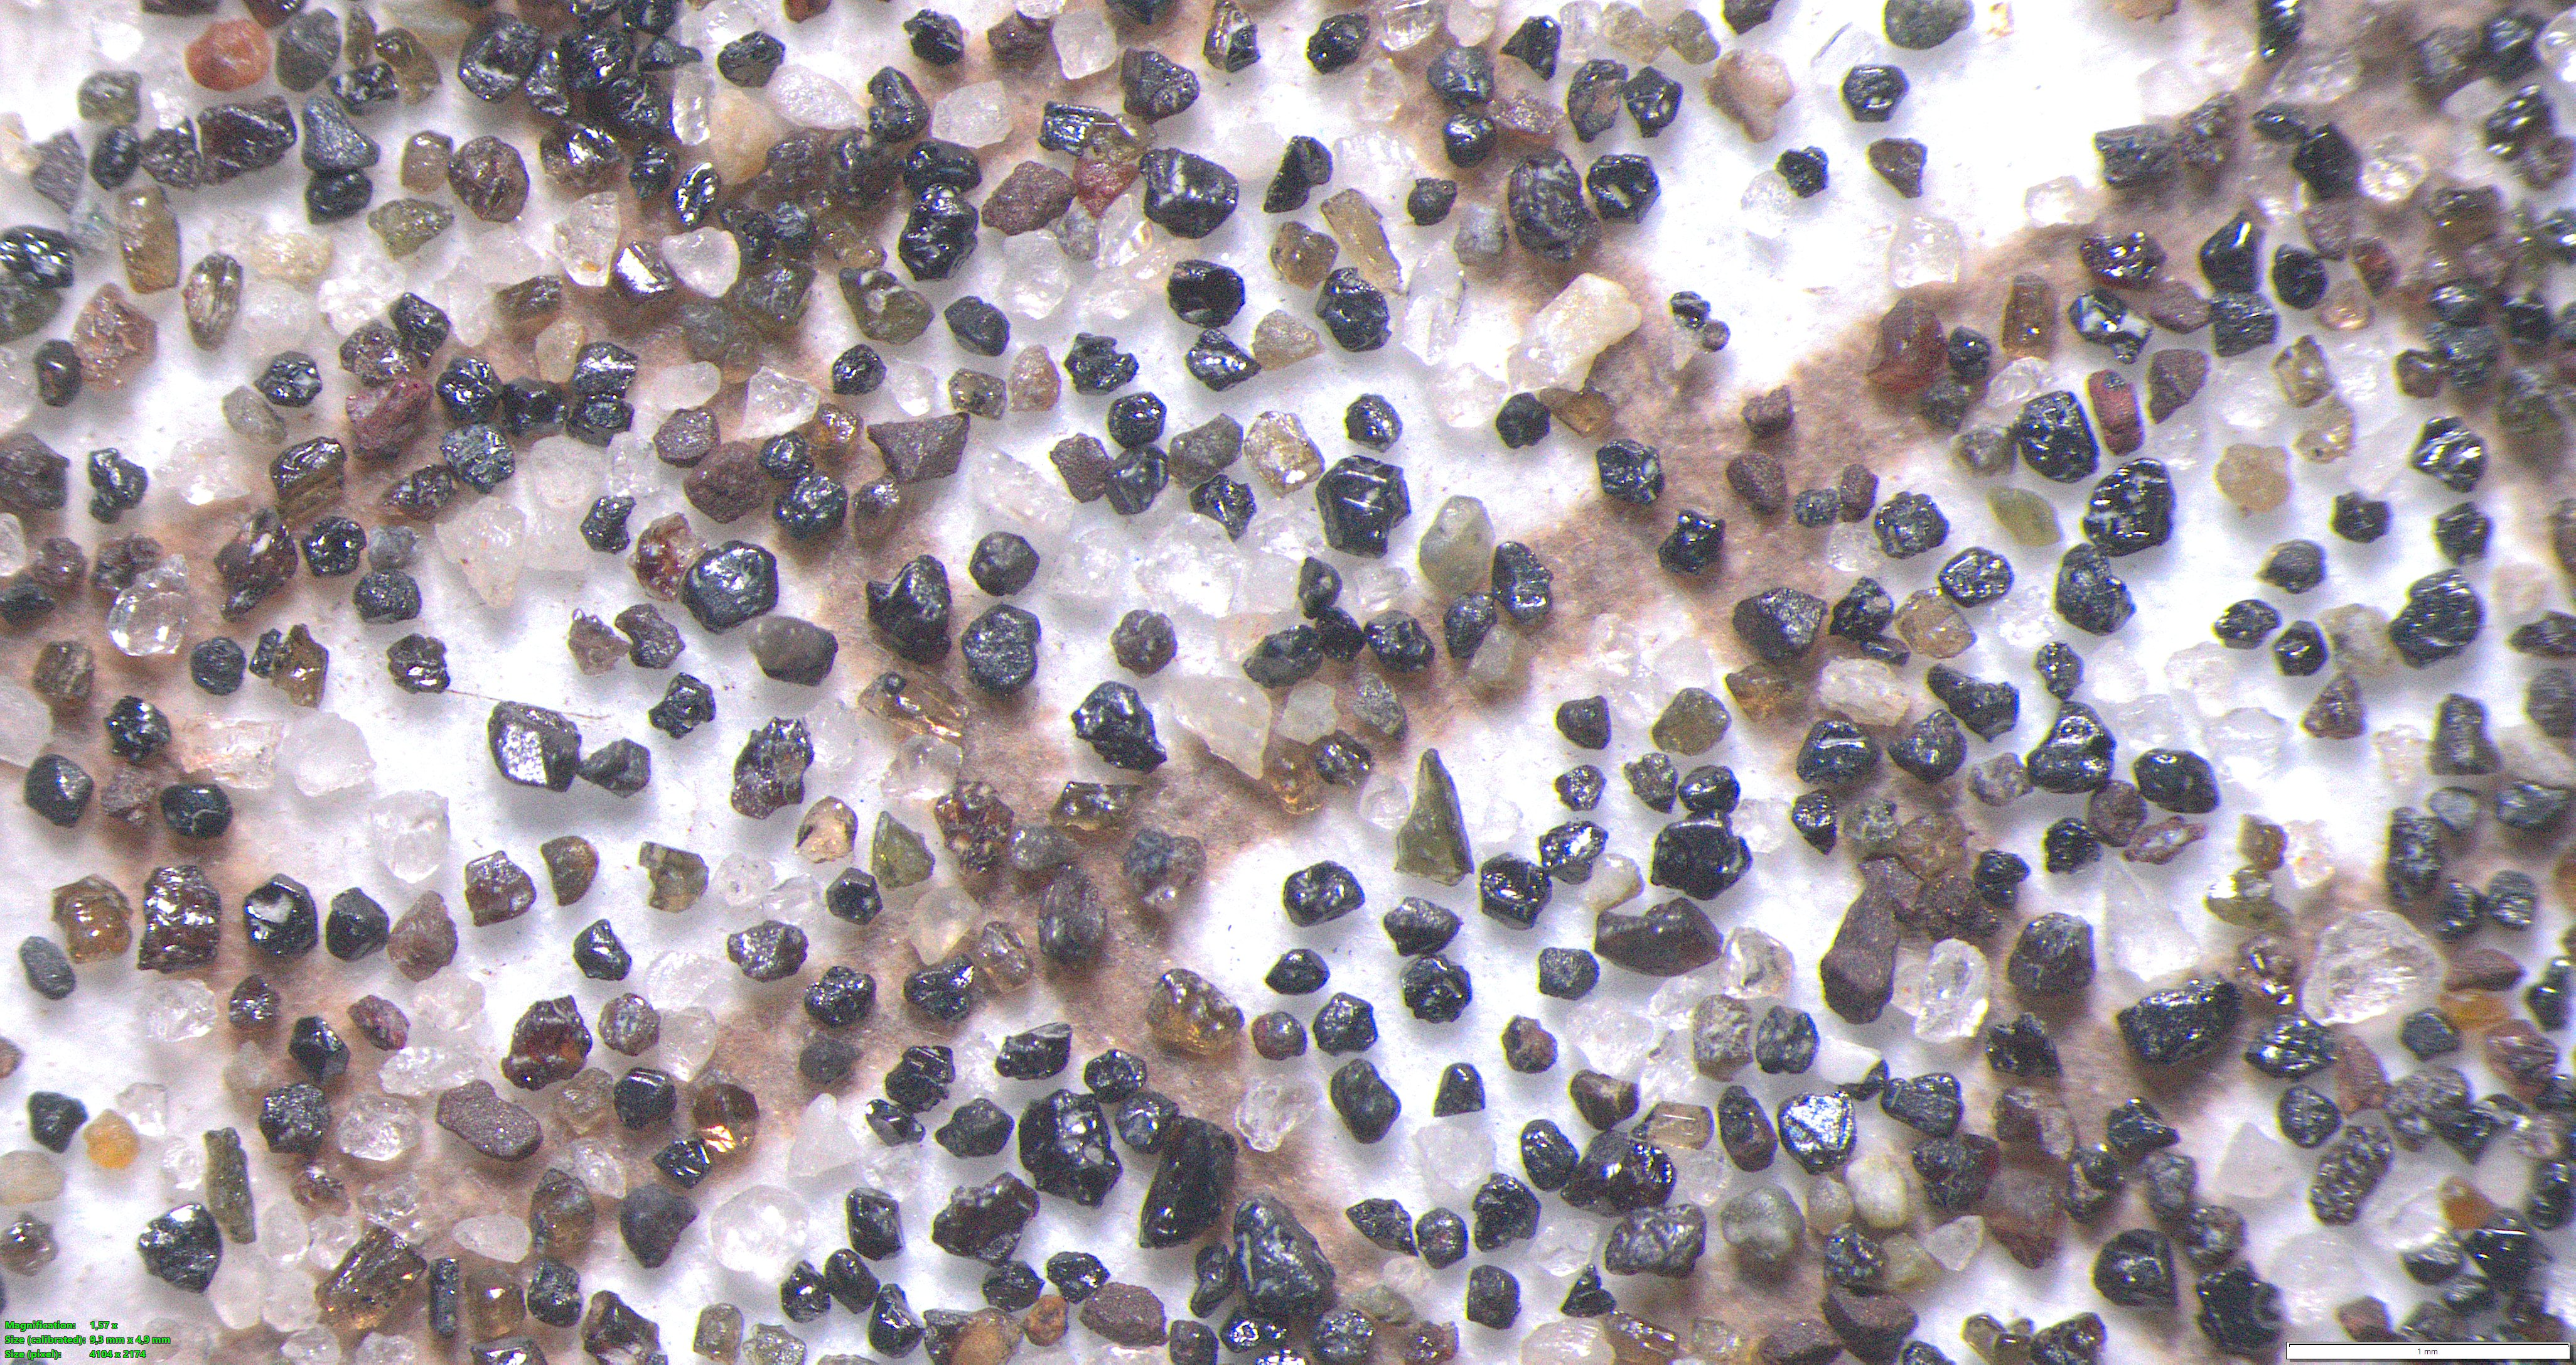
\includegraphics[width=\textwidth]{figure/tiles_285-25100F.jpg}
%         \caption{Citra Original Sebelum \textit{Tiling}}
%         \label{fig:3.TilingOriginal}
%     \end{subfigure}
    
%     \vskip\baselineskip
    
%     % 4 gambar sejajar satu baris
%     \begin{subfigure}[b]{0.24\textwidth}
%         \centering
%         \includegraphics[width=\textwidth]{figure/285-25100F_tile0.png}
%         \caption{Bagian 1}
%         \label{fig:3.Tile1}
%     \end{subfigure}
%     \hfill
%     \begin{subfigure}[b]{0.24\textwidth}
%         \centering
%         \includegraphics[width=\textwidth]{figure/285-25100F_tile1.png}
%         \caption{Bagian 2}
%         \label{fig:3.Tile2}
%     \end{subfigure}
%     \hfill
%     \begin{subfigure}[b]{0.24\textwidth}
%         \centering
%         \includegraphics[width=\textwidth]{figure/285-25100F_tile2.png}
%         \caption{Bagian 3}
%         \label{fig:3.Tile3}
%     \end{subfigure}
%     \hfill
%     \begin{subfigure}[b]{0.24\textwidth}
%         \centering
%         \includegraphics[width=\textwidth]{figure/285-25100F_tile3.png}
%         \caption{Bagian 4}
%         \label{fig:3.Tile4}
%     \end{subfigure}

%     \caption{Proses Pembagian Citra (\textit{Image Tiling}) Menjadi Grid $2 \times 2$}
%     \label{fig:3.HasilTilingData}
% \end{figure}


% \subsubsection{\textit{Resize}}
% Pada tahapan ini, data diproses untuk menghasilkan kumpulan data dengan ukuran yang seragam, yaitu  $1920 \times 1080$ piksel. Ukuran data dipilih berdasarkan resolusi asli citra mikroskop yang diperoleh dari Laboratorium Eksplorasi PT. Timah Tbk., yakni terdapat dua ukuran yaitu $1920 \times 1080$ piksel dan $4104 \times 2174$ piksel. Penyeragaman ukuran citra dilakukan agar seluruh data memiliki dimensi yang konsisten, sehingga memudahkan proses pelatihan model dan menghindari ketidaksesuaian resolusi yang dapat memengaruhi hasil segmentasi. Selain itu, pemilihan ukuran $1920 \times 1080$ piksel juga dipertimbangkan untuk menjaga keseimbangan antara kualitas detail citra dan efisiensi komputasi selama proses pemrosesan data. Contoh hasil perubahan resolusi citra dari ukuran awal menjadi ukuran seragam ditunjukkan pada Gambar \ref{fig:3.HasilResizeData} berikut. \par

% \begin{figure}[H]
%     \centering
%     % Baris pertama: dua gambar sejajar
%     \begin{subfigure}[b]{0.475\textwidth}
%         \centering
%         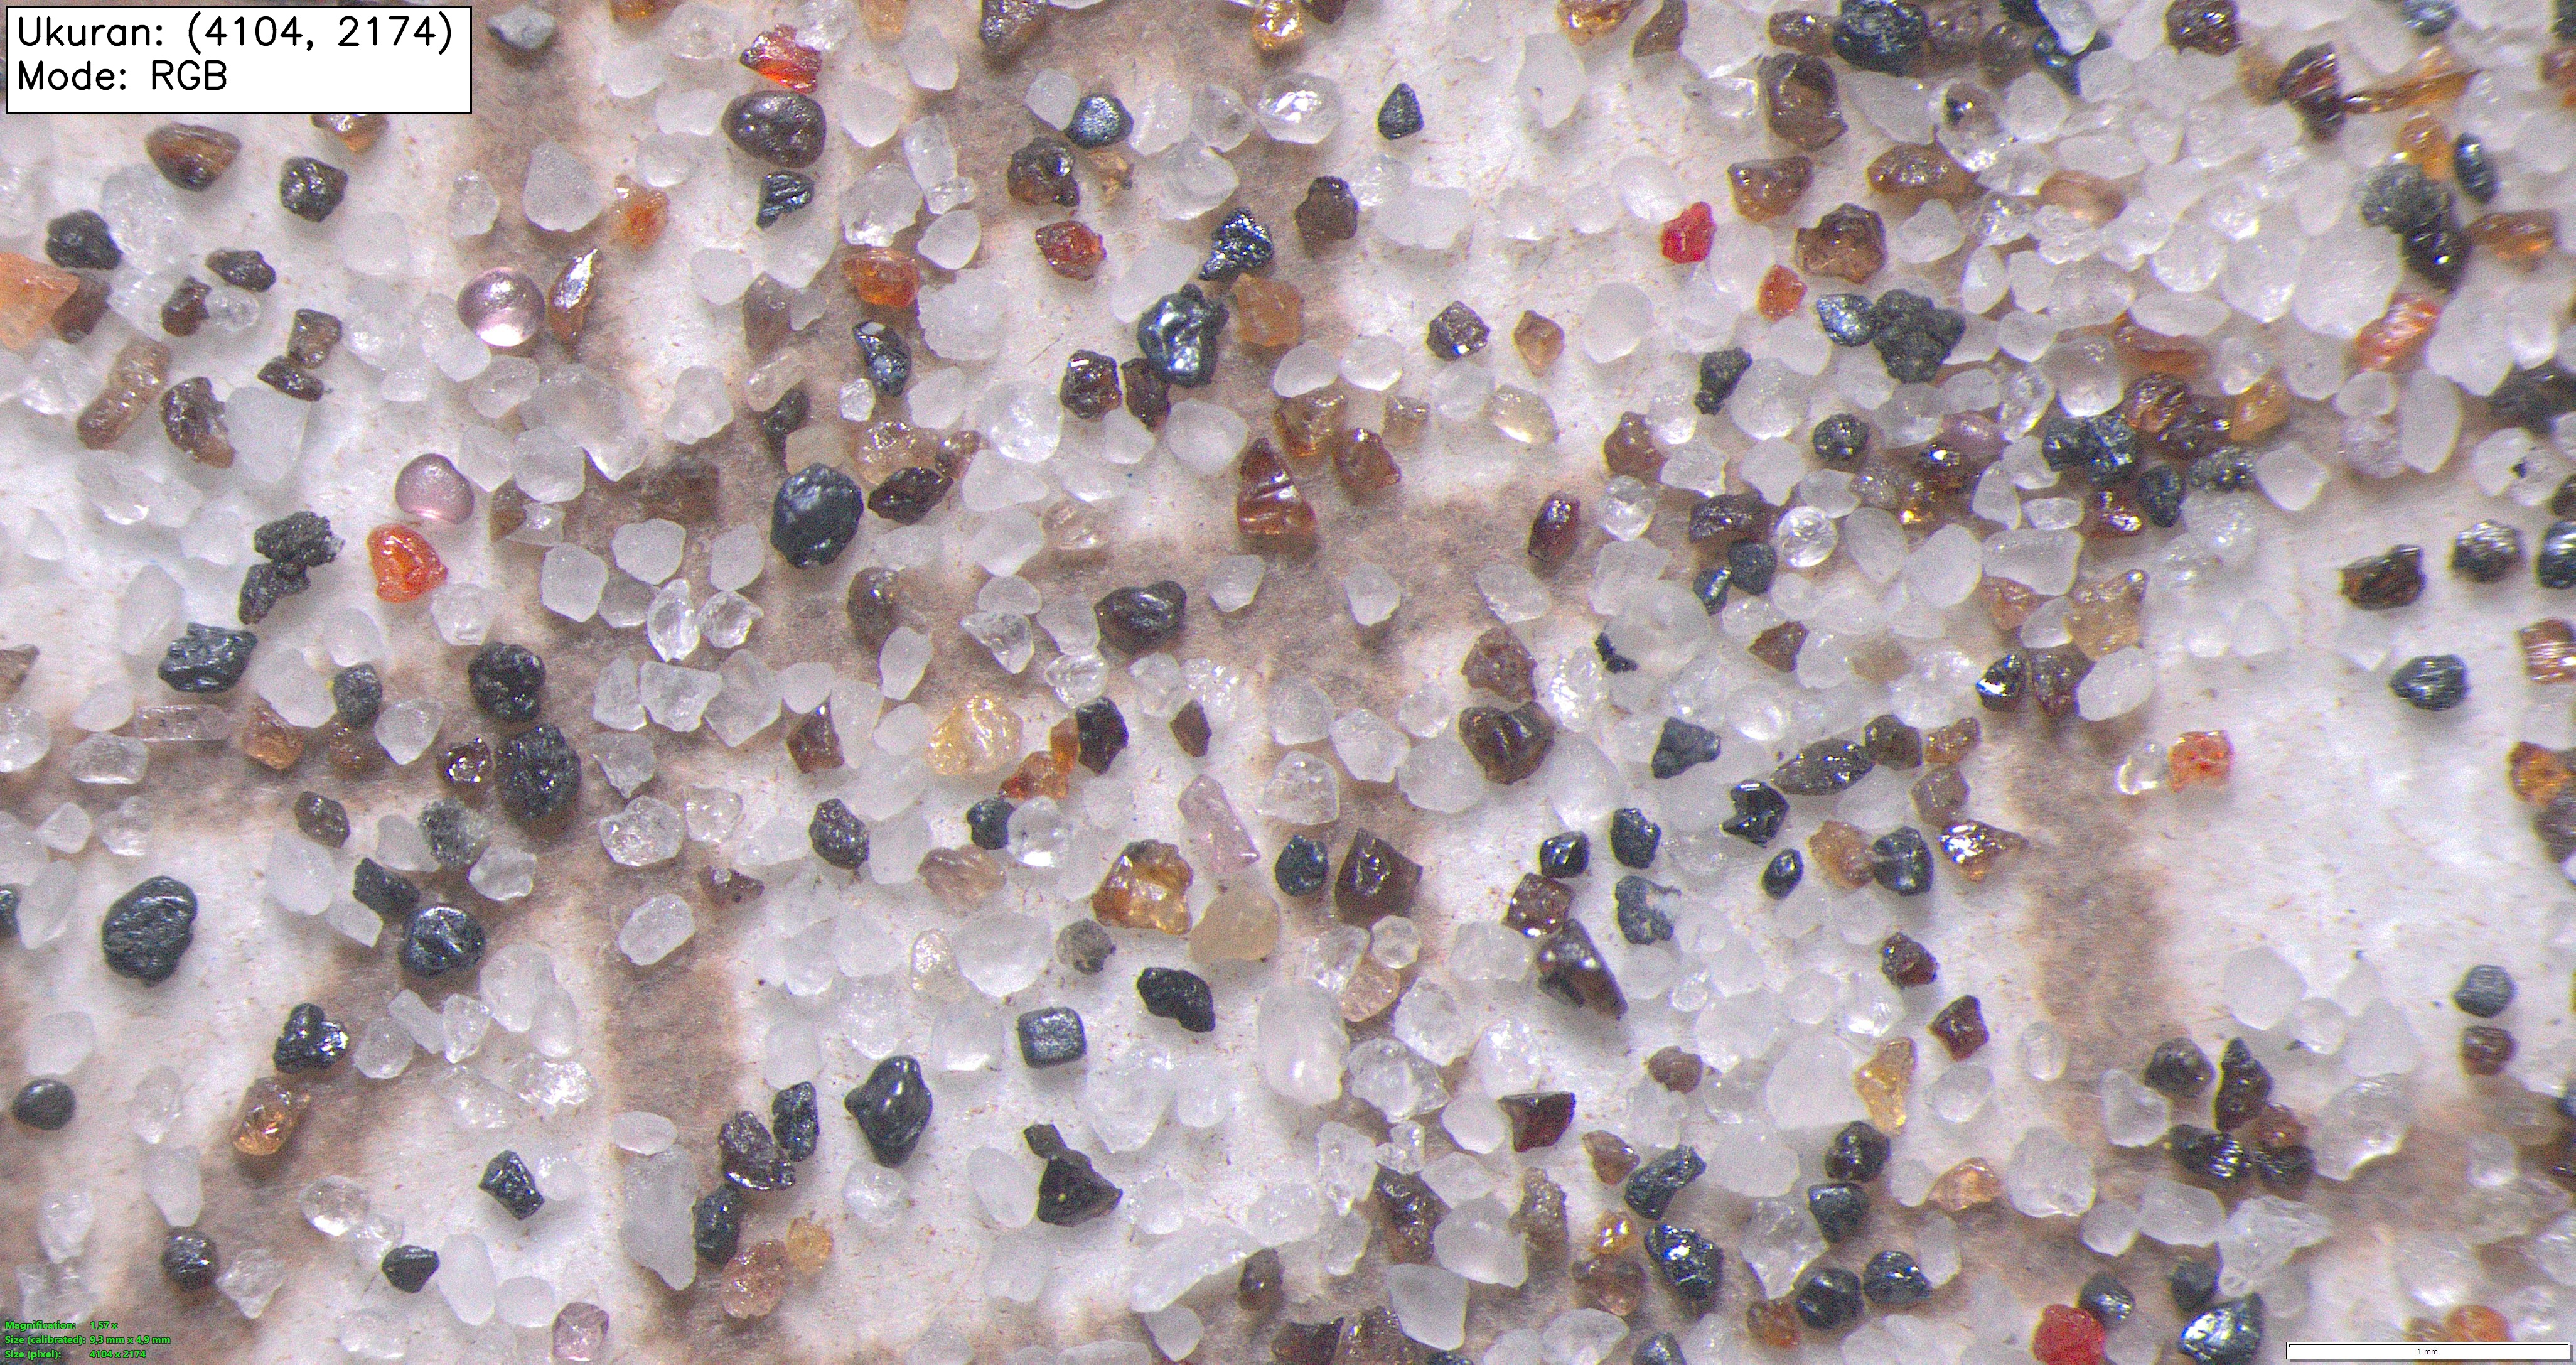
\includegraphics[width=\textwidth]{figure/hasilResizeAsli_denganKeterangan.jpg}
%         \caption{Citra Awal dengan resolusi $4104 \times 2174$ piksel}
%         \label{fig:3.ResizeAwal}
%     \end{subfigure}
%     \hfill
%     \begin{subfigure}[b]{0.475\textwidth}
%         \centering
%         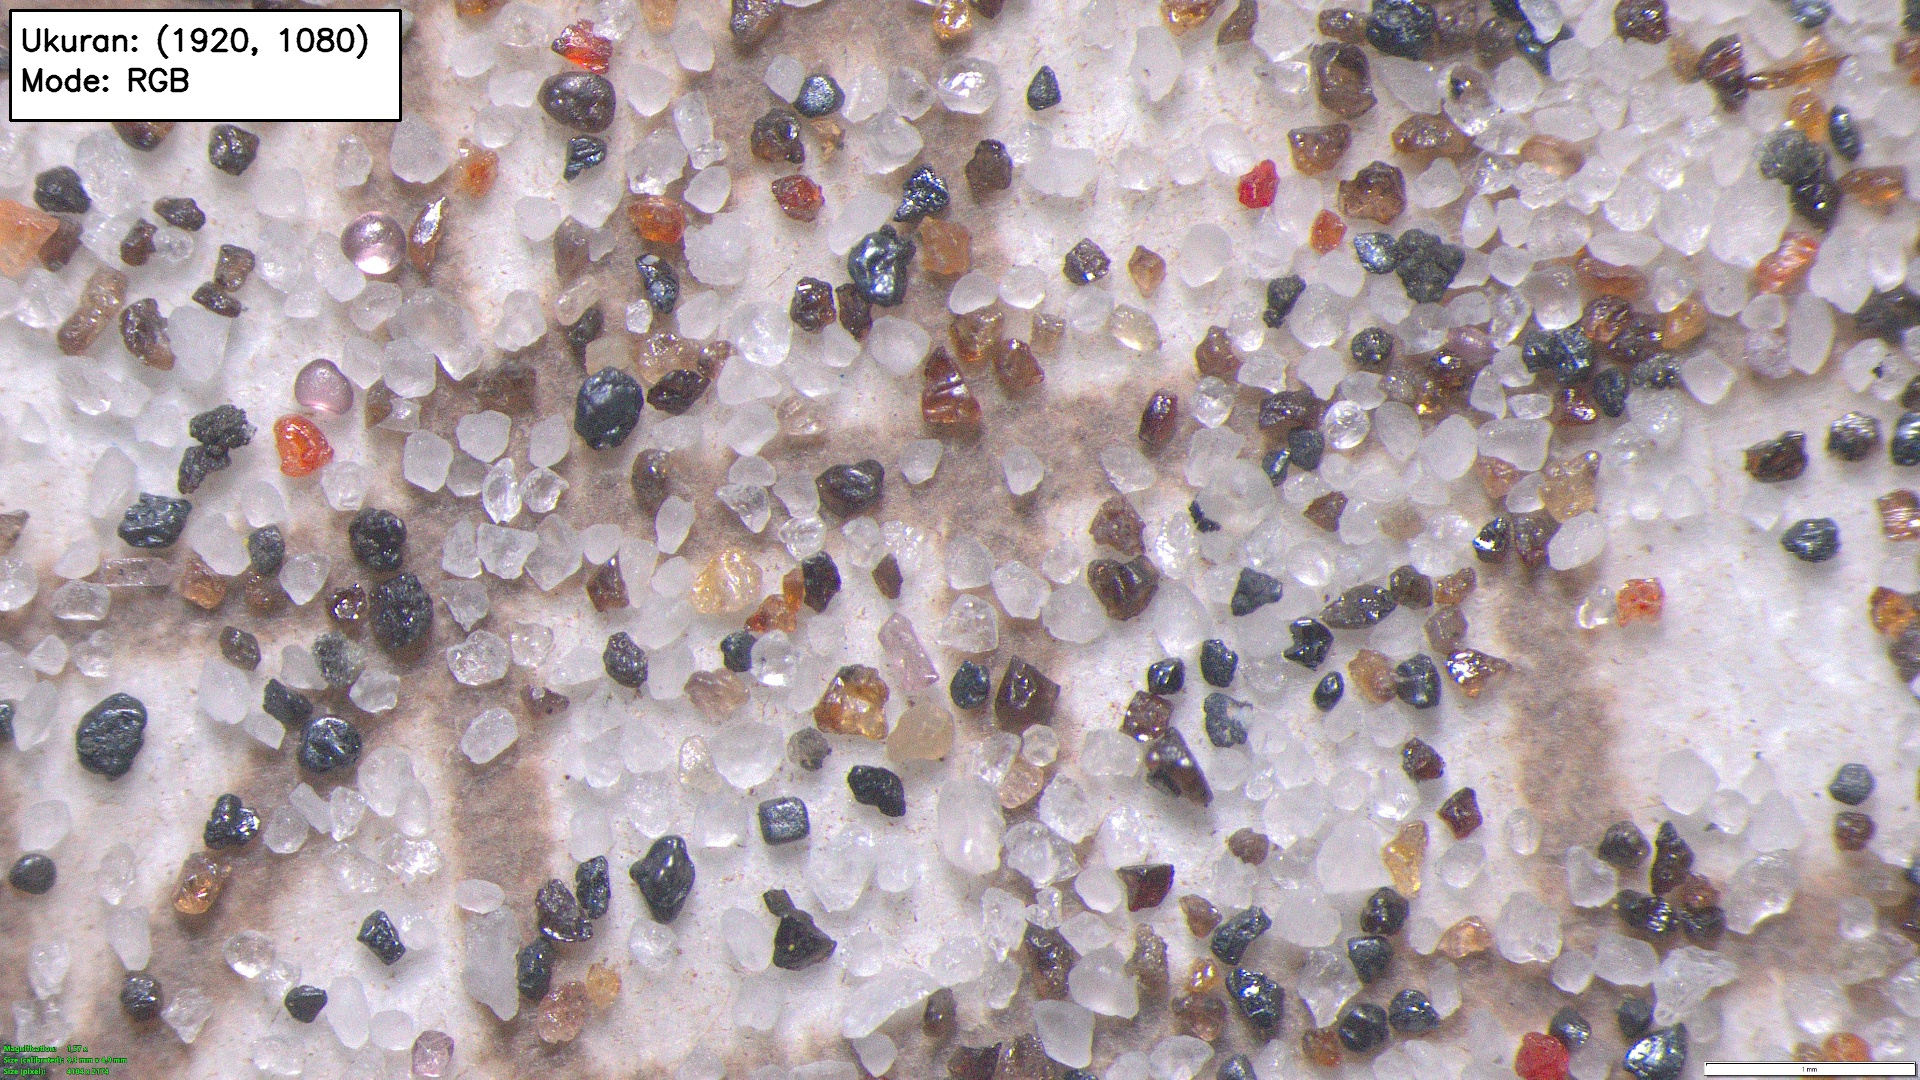
\includegraphics[width=\textwidth]{figure/hasilResize_denganKeterangan.jpg}
%         \caption{Hasil Resize dengan resolusi $1920 \times 1080$ piksel}
%         \label{fig:3.ResizeAkhir}
%     \end{subfigure}

% 	\caption{Hasil Resize Data}
%     \label{fig:3.HasilResizeData}
% \end{figure}

\subsubsection{Augmentasi Data}
Augmentasi yang dilakukan pada penelitian ini meliputi teknik \textit{flip}, \textit{rotate}, dan penambahan \textit{Gaussian noise}. Teknik-teknik ini diterapkan untuk memperkaya variasi data pelatihan, sehingga model dapat belajar mengenali objek mineral kasiterit dalam berbagai kondisi visual yang berbeda. Berikut merupakan penjelasan dari masing-masing teknik augmentasi yang diterapkan.\par

\subsubsection*{\textnormal{1. \textit{Flip}}}
Pada tahapan ini, data citra mikroskop diolah dengan menerapkan teknik augmentasi \textit{flip} yang membalik citra baik secara \textit{horizontal} maupun \textit{vertikal} untuk menambah variasi data pelatihan \cite{thesisNova}. Teknik ini digunakan agar model dapat mengenali objek mineral kasiterit dari berbagai orientasi tanpa kehilangan informasi penting pada citra. Dengan adanya \textit{HorizontalFlip} dan \textit{VerticalFlip} yang diterapkan secara acak, model menjadi lebih \textit{robust} terhadap perubahan posisi atau arah objek pada citra mikroskop. Contoh hasil penerapan teknik \textit{flip} secara \textit{horizontal} dan \textit{vertikal} ditunjukkan pada Gambar \ref{fig:3.HasilFlipData} berikut.\par

\begin{figure}[H]
    \centering
    % Baris pertama: dua gambar sejajar
    \begin{subfigure}[b]{0.475\textwidth}
        \centering
        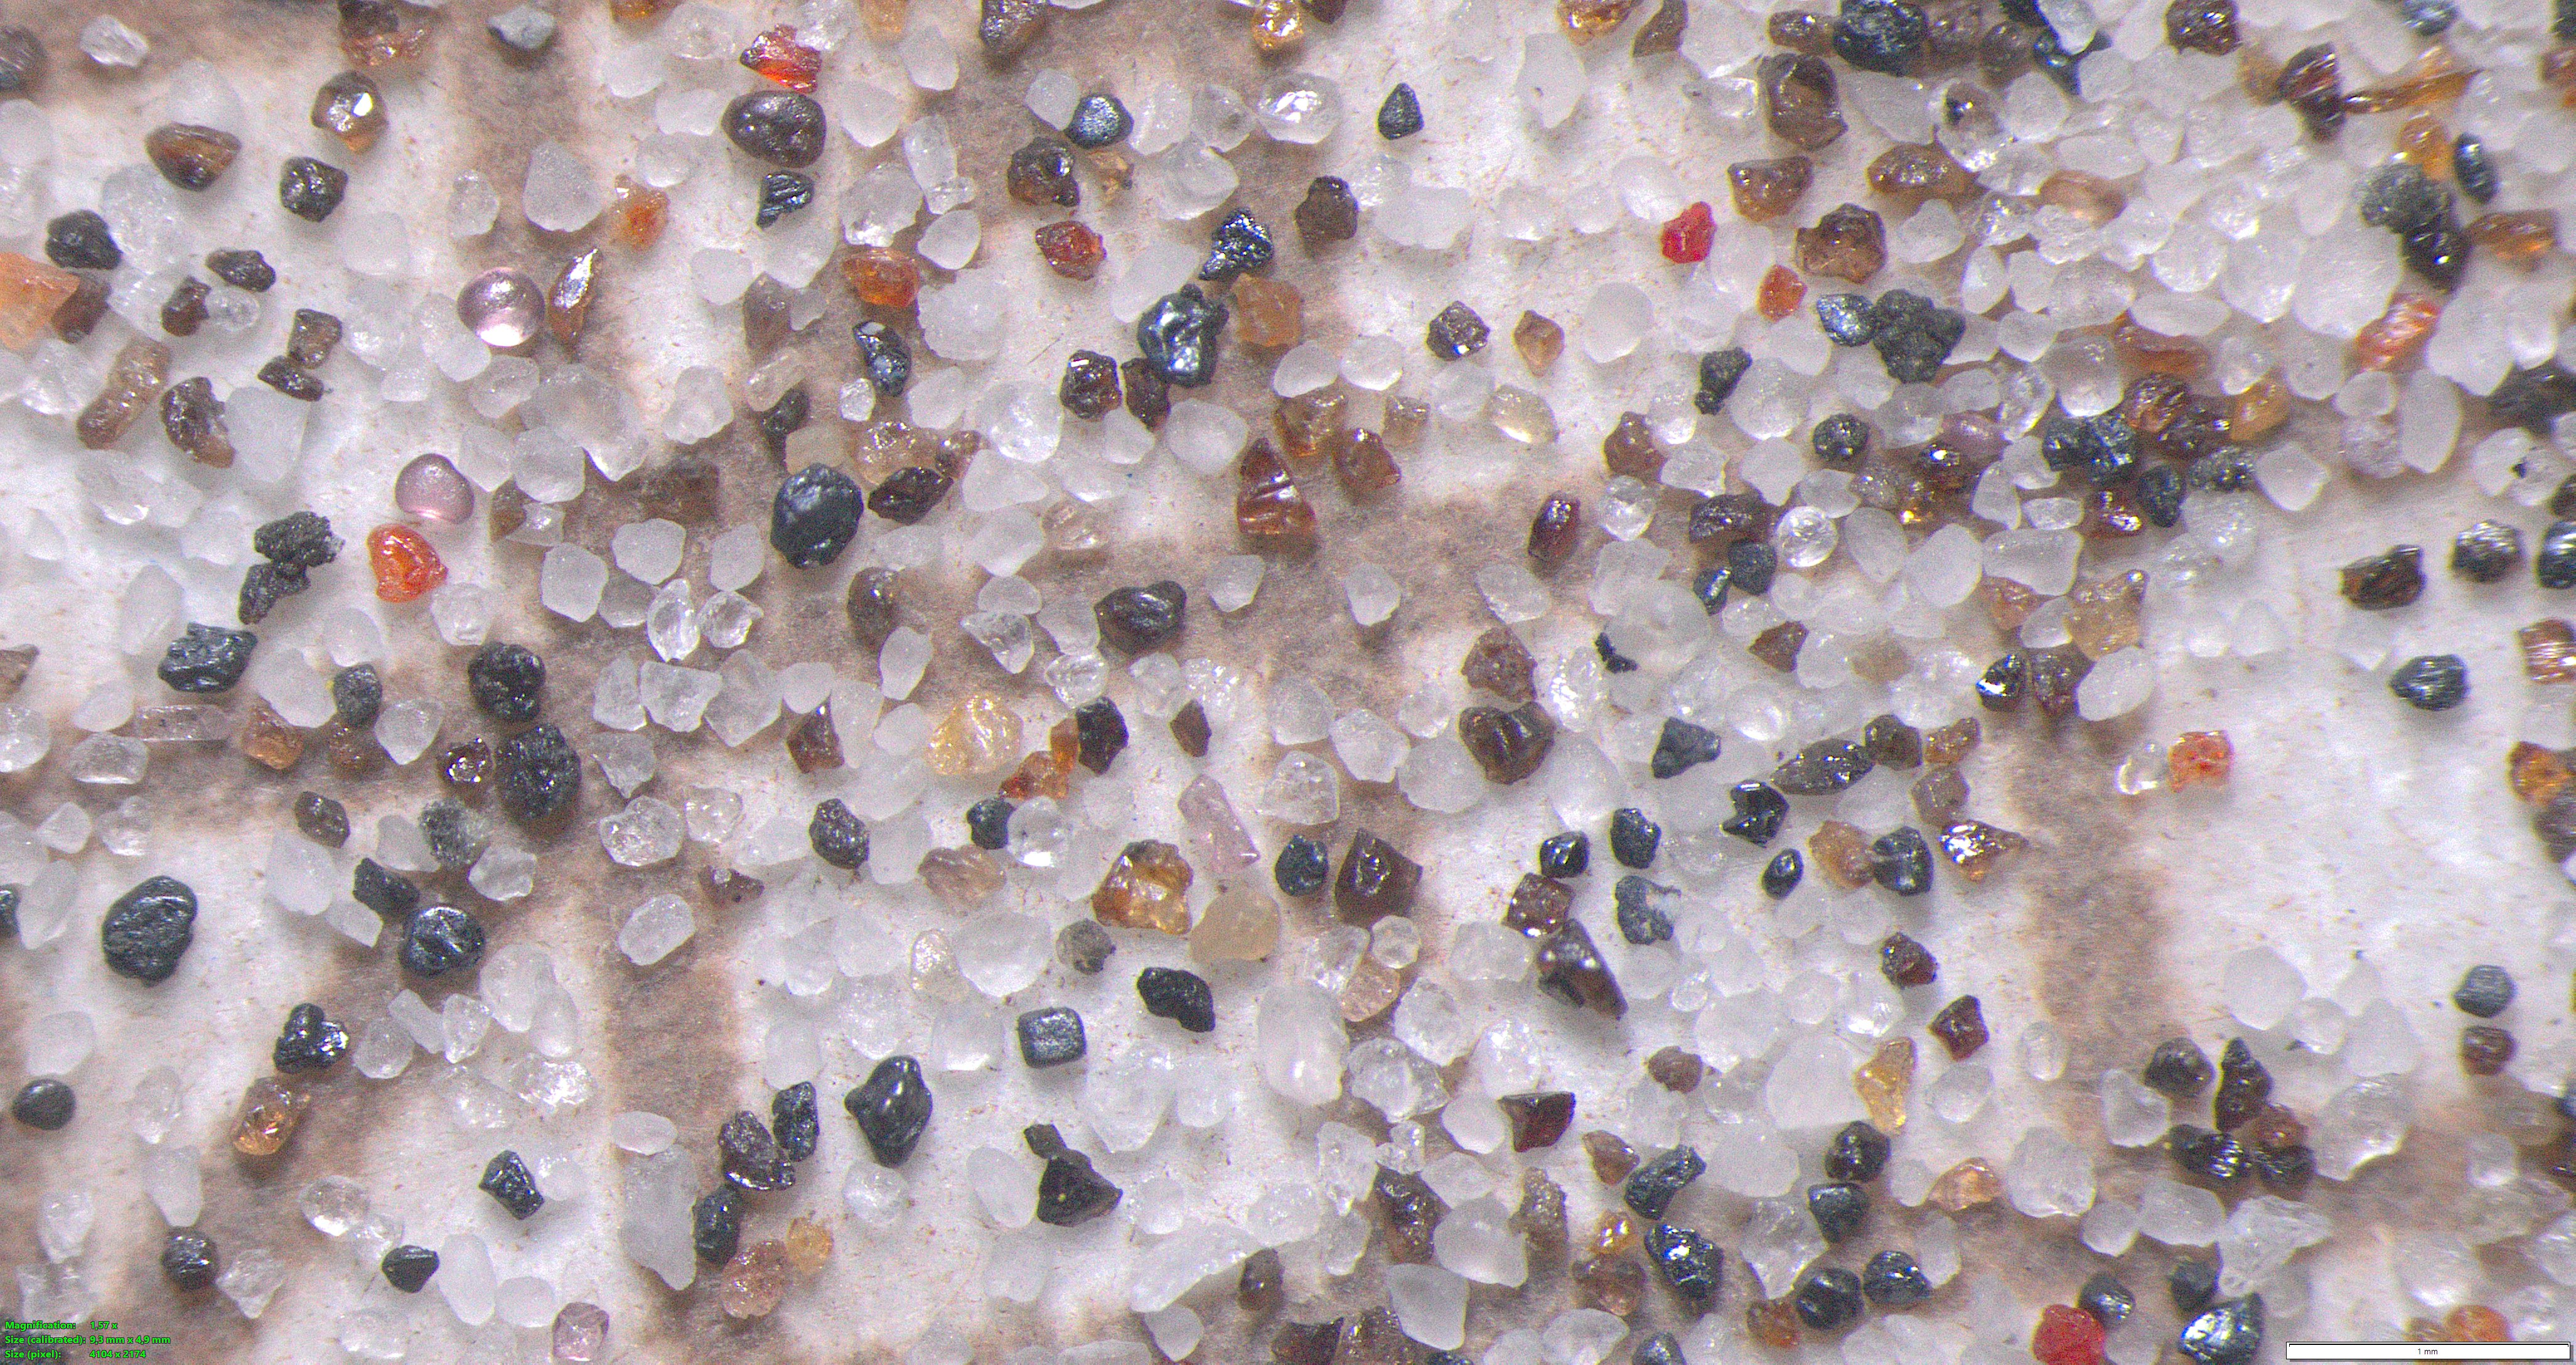
\includegraphics[width=\textwidth]{figure/sebeleumResize.jpg}
        \caption{Citra Awal tanpa \textit{Flip}}
        \label{fig:3.CitraAwalFlip}
    \end{subfigure}
    
    % Baris kedua: satu gambar di bawah tengah
    \vskip\baselineskip
    \begin{subfigure}[b]{0.475\textwidth}
        \centering
        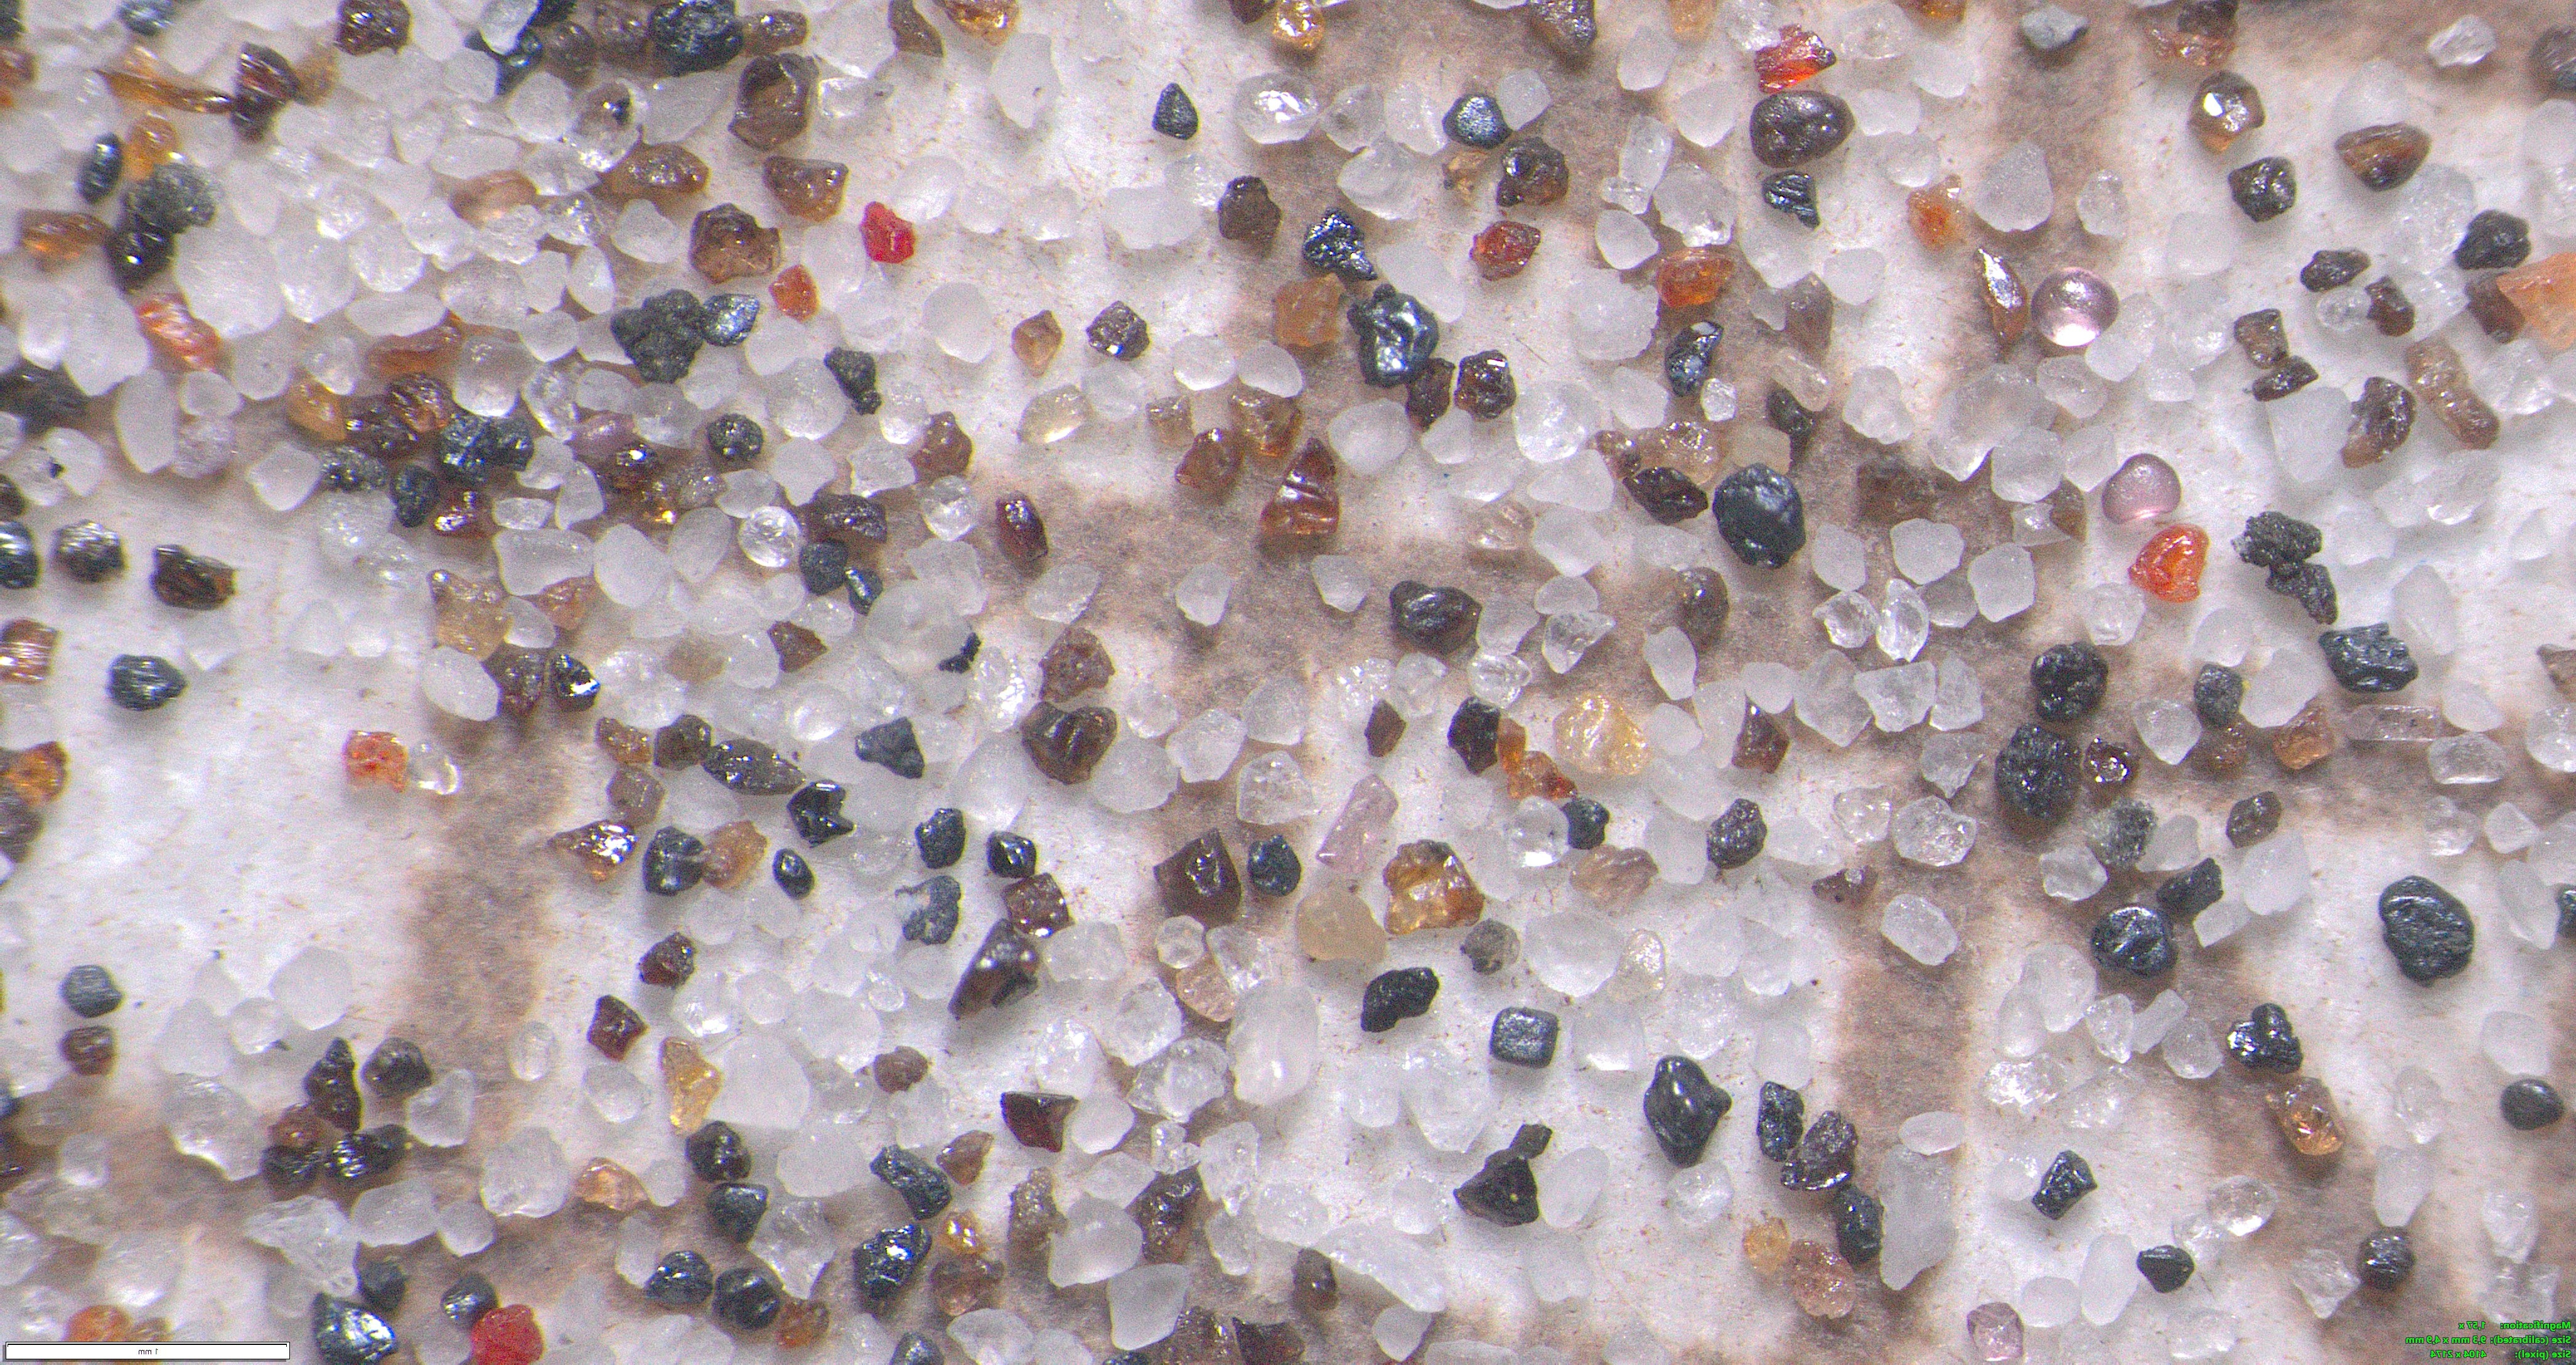
\includegraphics[width=\textwidth]{figure/hasilFlipHorizontal.jpg}
        \caption{Hasil \textit{Flip} Horizontal ($\curvearrowright$)}
        \label{fig:3.hasilFlipHorizontal}
    \end{subfigure}
    \hfill
    \begin{subfigure}[b]{0.475\textwidth}
        \centering
        \includegraphics[width=\textwidth]{figure/hasilFlipVertical.jpg}
        % \caption{Hasil \textit{Flip} Vertical ($\shortdownarrow$)}
        \caption{Hasil \textit{Flip} Vertical (\protect$\downarrow$)}
        % \caption{Hasil \textit{Flip} Vertical ($\downarrow$)}

        \label{fig:3.hasilFlipVertical}
    \end{subfigure}
    \caption{Hasil \textit{Flip} Data}
    \label{fig:3.HasilFlipData}
\end{figure}

\subsubsection*{\textnormal{2. \textit{Rotate}}}
Pada tahapan ini, data citra mikroskop diolah dengan menerapkan teknik augmentasi \textit{random rotation} yang memutar citra pada rentang sudut tertentu, seperti $-15^{\circ}$ hingga $+15^{\circ}$ untuk menambah variasi data pelatihan \cite{RotateBatik}. Teknik ini digunakan agar model dapat mengenali objek mineral kasiterit dari berbagai sudut pandang tanpa kehilangan informasi penting pada citra. Tujuan dari \textit{rotate} ini adalah untuk memperkaya sudut pandang data dan membantu model dalam mengenali objek mineral kasiterit yang mungkin muncul dalam orientasi berbeda di bawah mikroskop. Contoh hasil penerapan teknik \textit{rotate} dengan sudut rotasi sebesar $15^{\circ}$ dapat dilihat pada Gambar \ref{fig:3.HasilRotateData} berikut. \par

\begin{figure}[H]
    \centering
    % Baris pertama: dua gambar sejajar
    \begin{subfigure}[b]{0.475\textwidth}
        \centering
        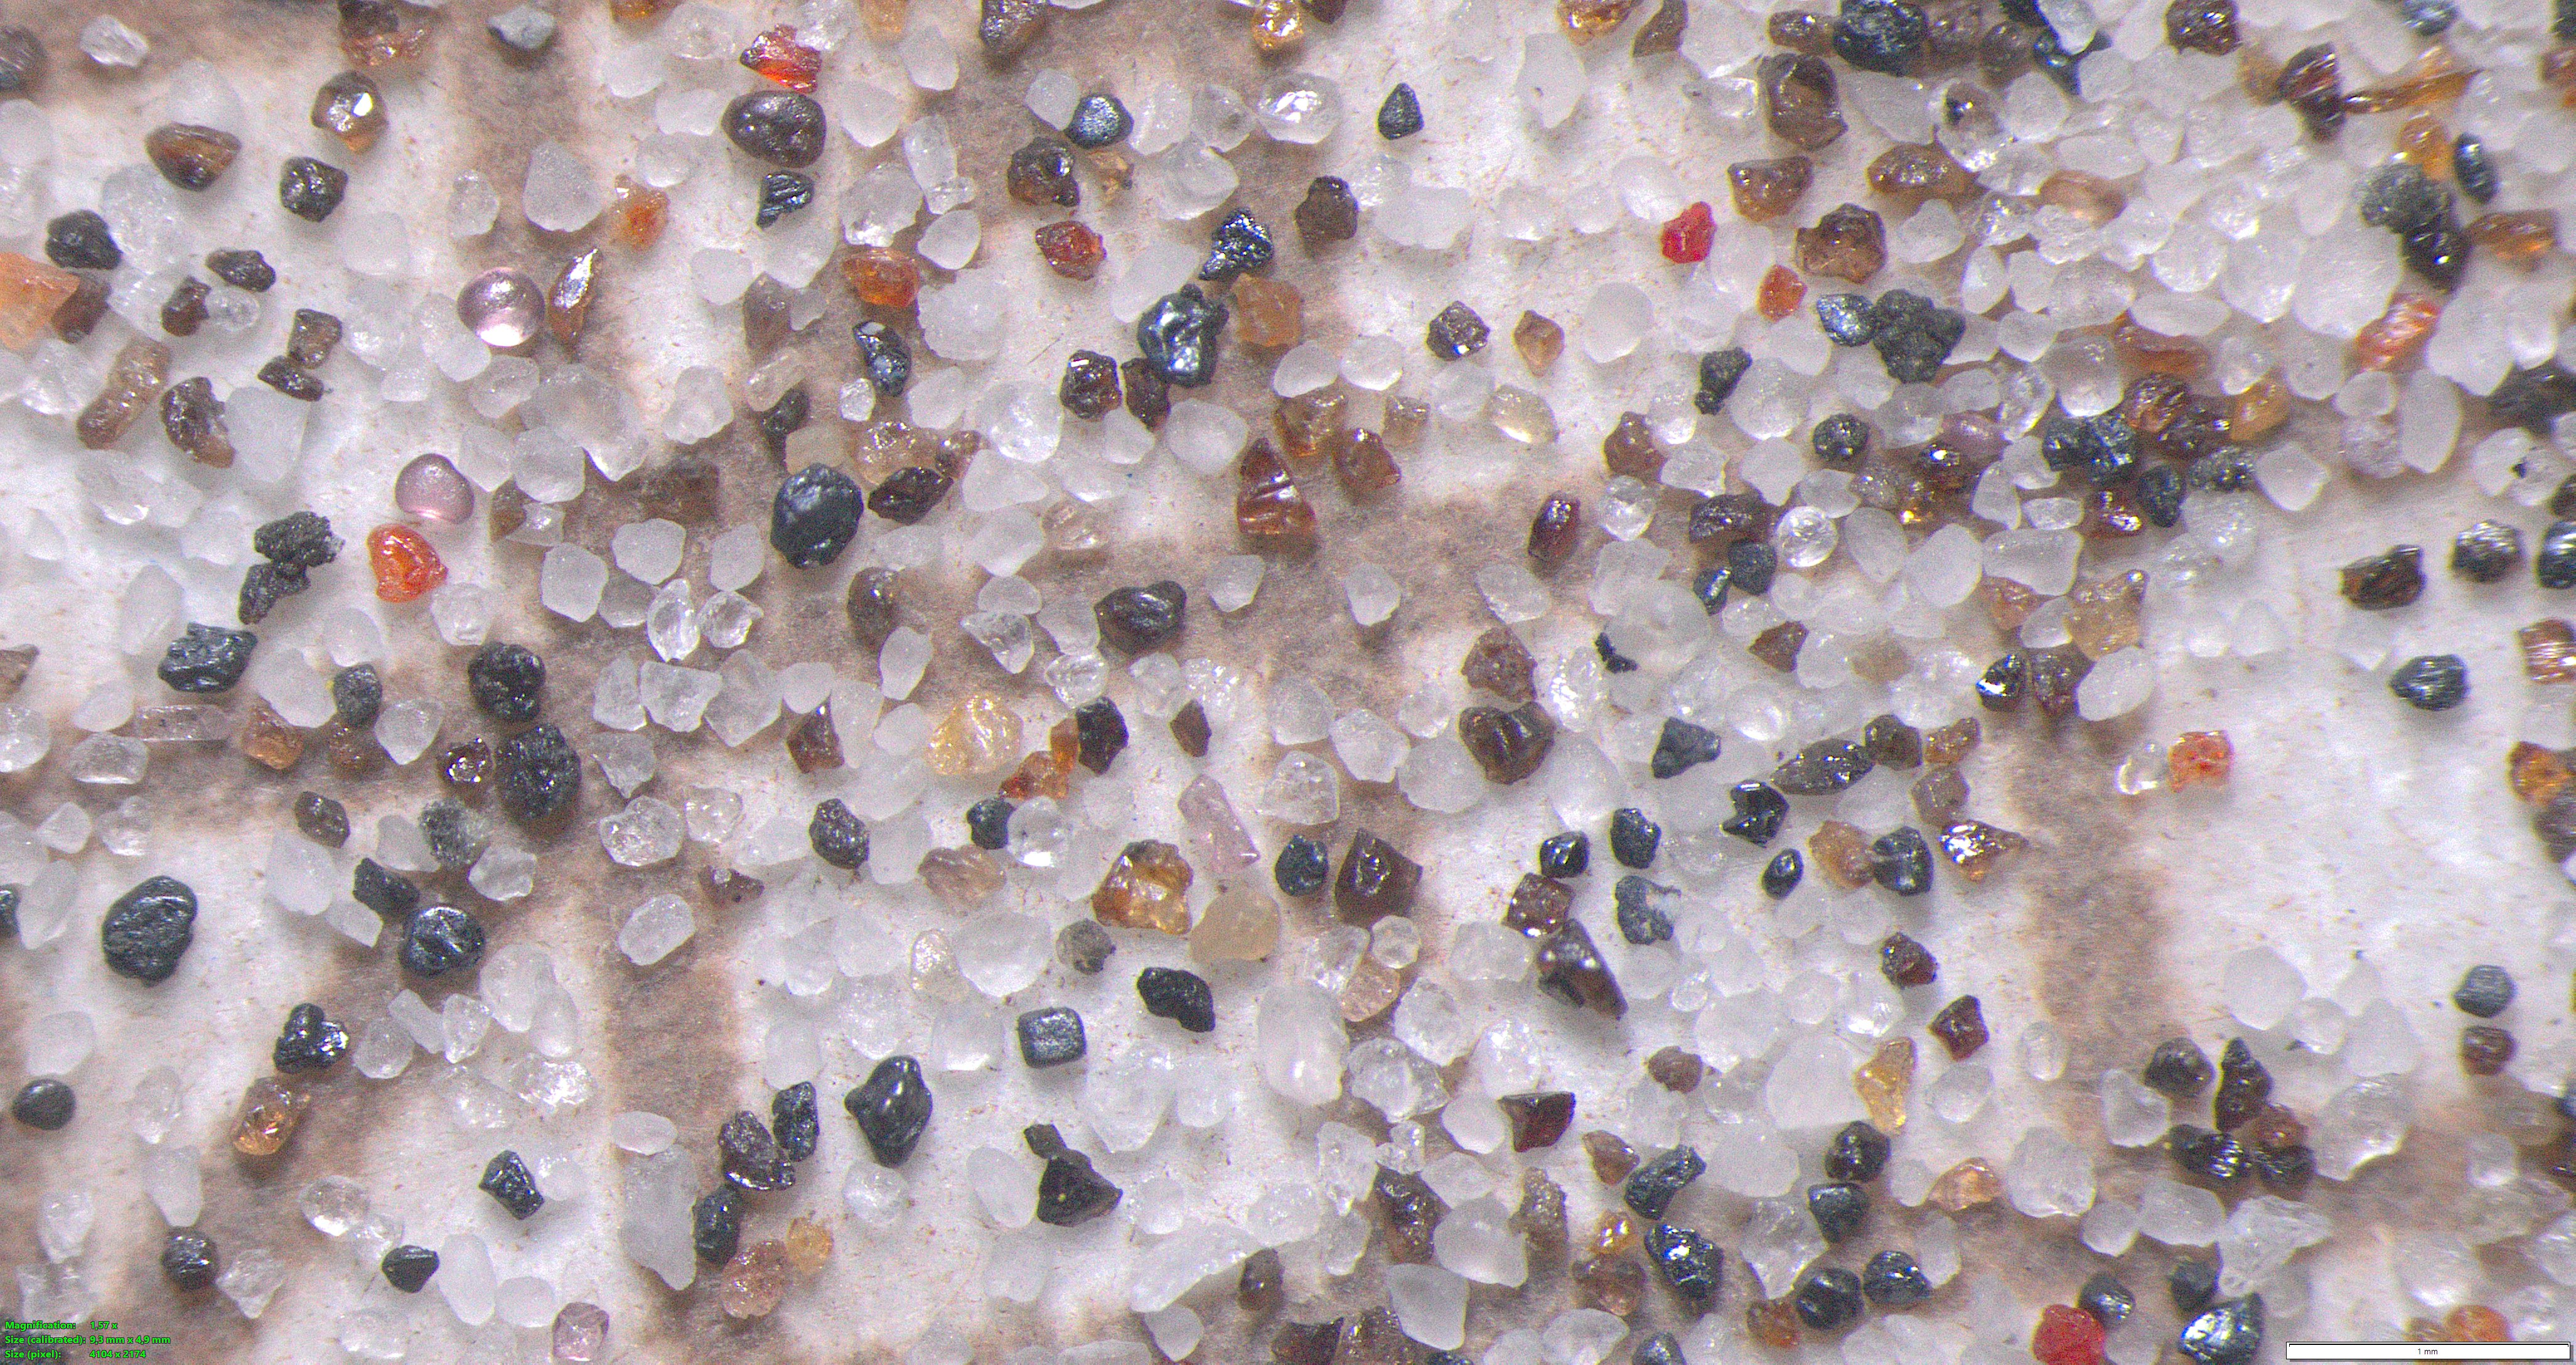
\includegraphics[width=\textwidth]{figure/sebeleumResize.jpg}
        \caption{Citra Awal tanpa \textit{Rotate}}
        \label{fig:3.RotateAwal}
    \end{subfigure}
    \hfill
    \begin{subfigure}[b]{0.475\textwidth}
        \centering
        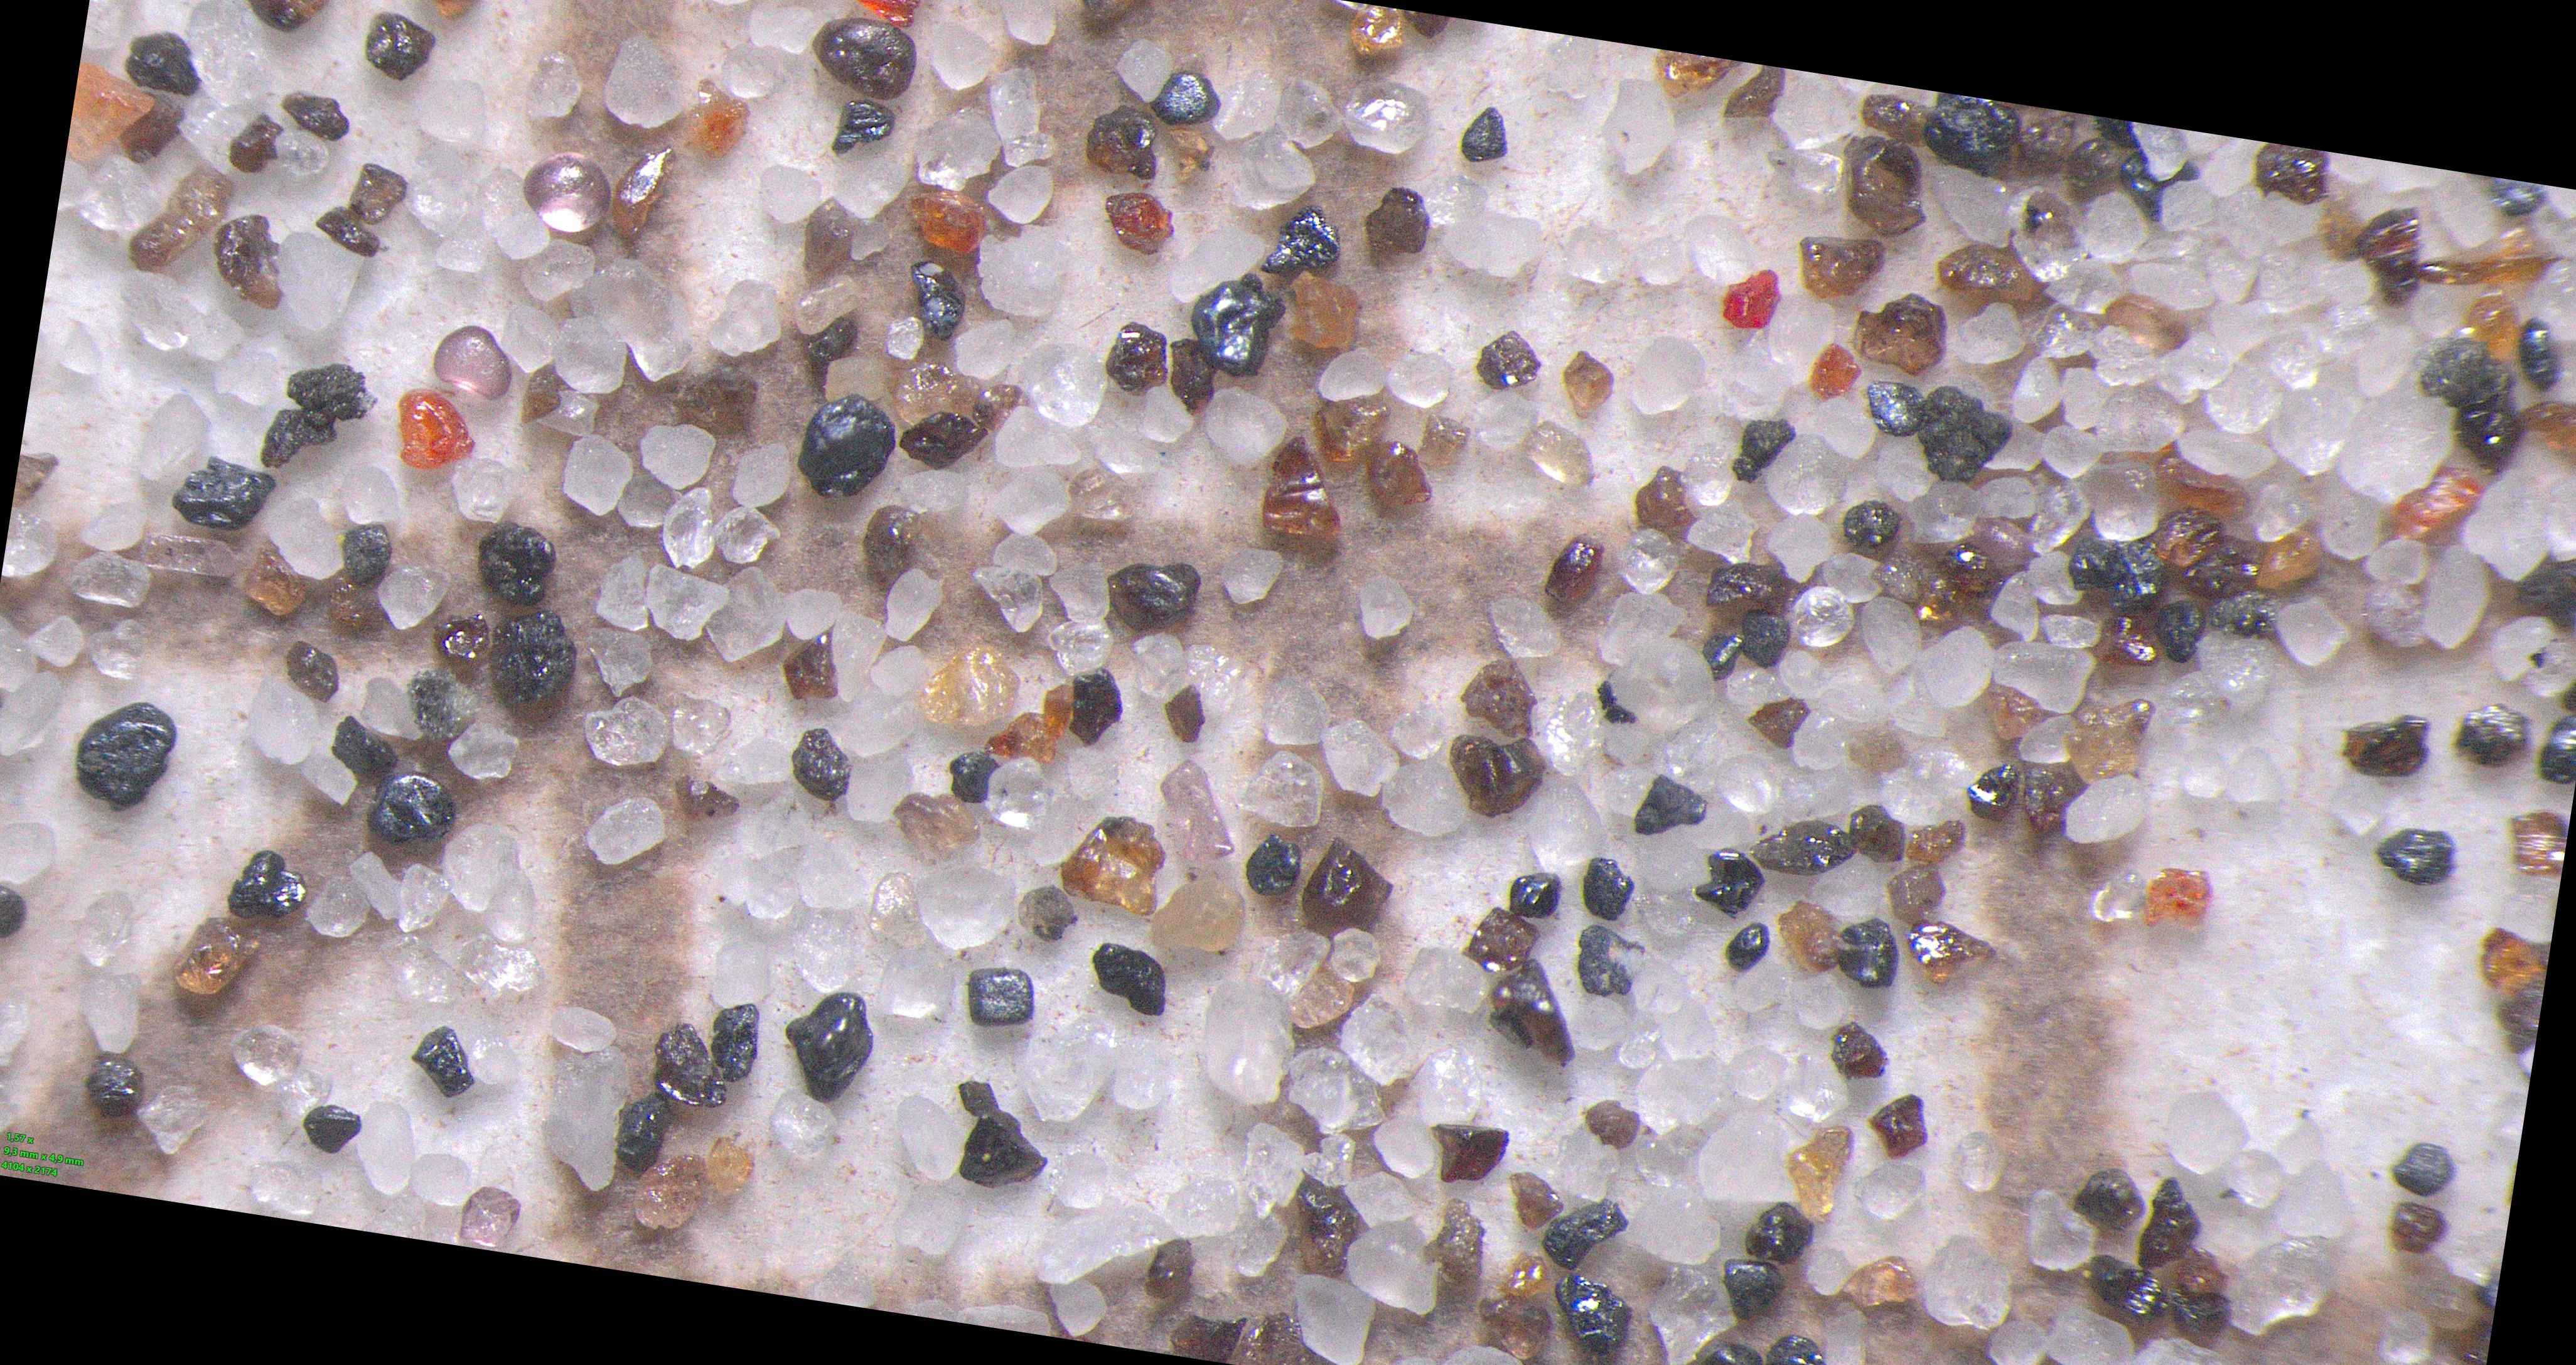
\includegraphics[width=\textwidth]{figure/hasilRotate.jpg}
        \caption{Hasil \textit{Rotate} dengan 15\textdegree}
        \label{fig:3.HasilRotate}
    \end{subfigure}

	\caption{Hasil \textit{Rotate} Data}
    \label{fig:3.HasilRotateData}
\end{figure}

\subsubsection*{\textnormal{3. \textit{Gaussian Noise}}}
Pada tahapan ini, data citra mikroskop diolah dengan menerapkan teknik augmentasi \textit{Gaussian noise} yang menambahkan derau acak pada citra untuk meningkatkan ketahanan model terhadap gangguan visual. Penambahan \textit{noise} dilakukan dengan intensitas rendah agar tidak mengubah karakteristik warna asli mineral, tetapi tetap memberikan variasi kecil yang dapat memperkuat kemampuan generalisasi model terhadap perubahan pencahayaan dan fluktuasi sensor. \textit{Gaussian noise} diterapkan menggunakan nilai variansi sebesar 0{,}2 \cite{GaussianNoise0.2}, sehingga derau yang ditambahkan bersifat halus dan tidak mengganggu struktur visual mineral kasiterit. Contoh hasil penerapan teknik \textit{Gaussian noise} dengan variansi 0{,}2 ditunjukkan pada Gambar \ref{fig:3.HasilGaussianNoiseData} berikut. \par

\begin{figure}[H]
    \centering
    % Baris pertama: dua gambar sejajar
    \begin{subfigure}[b]{0.475\textwidth}
        \centering
        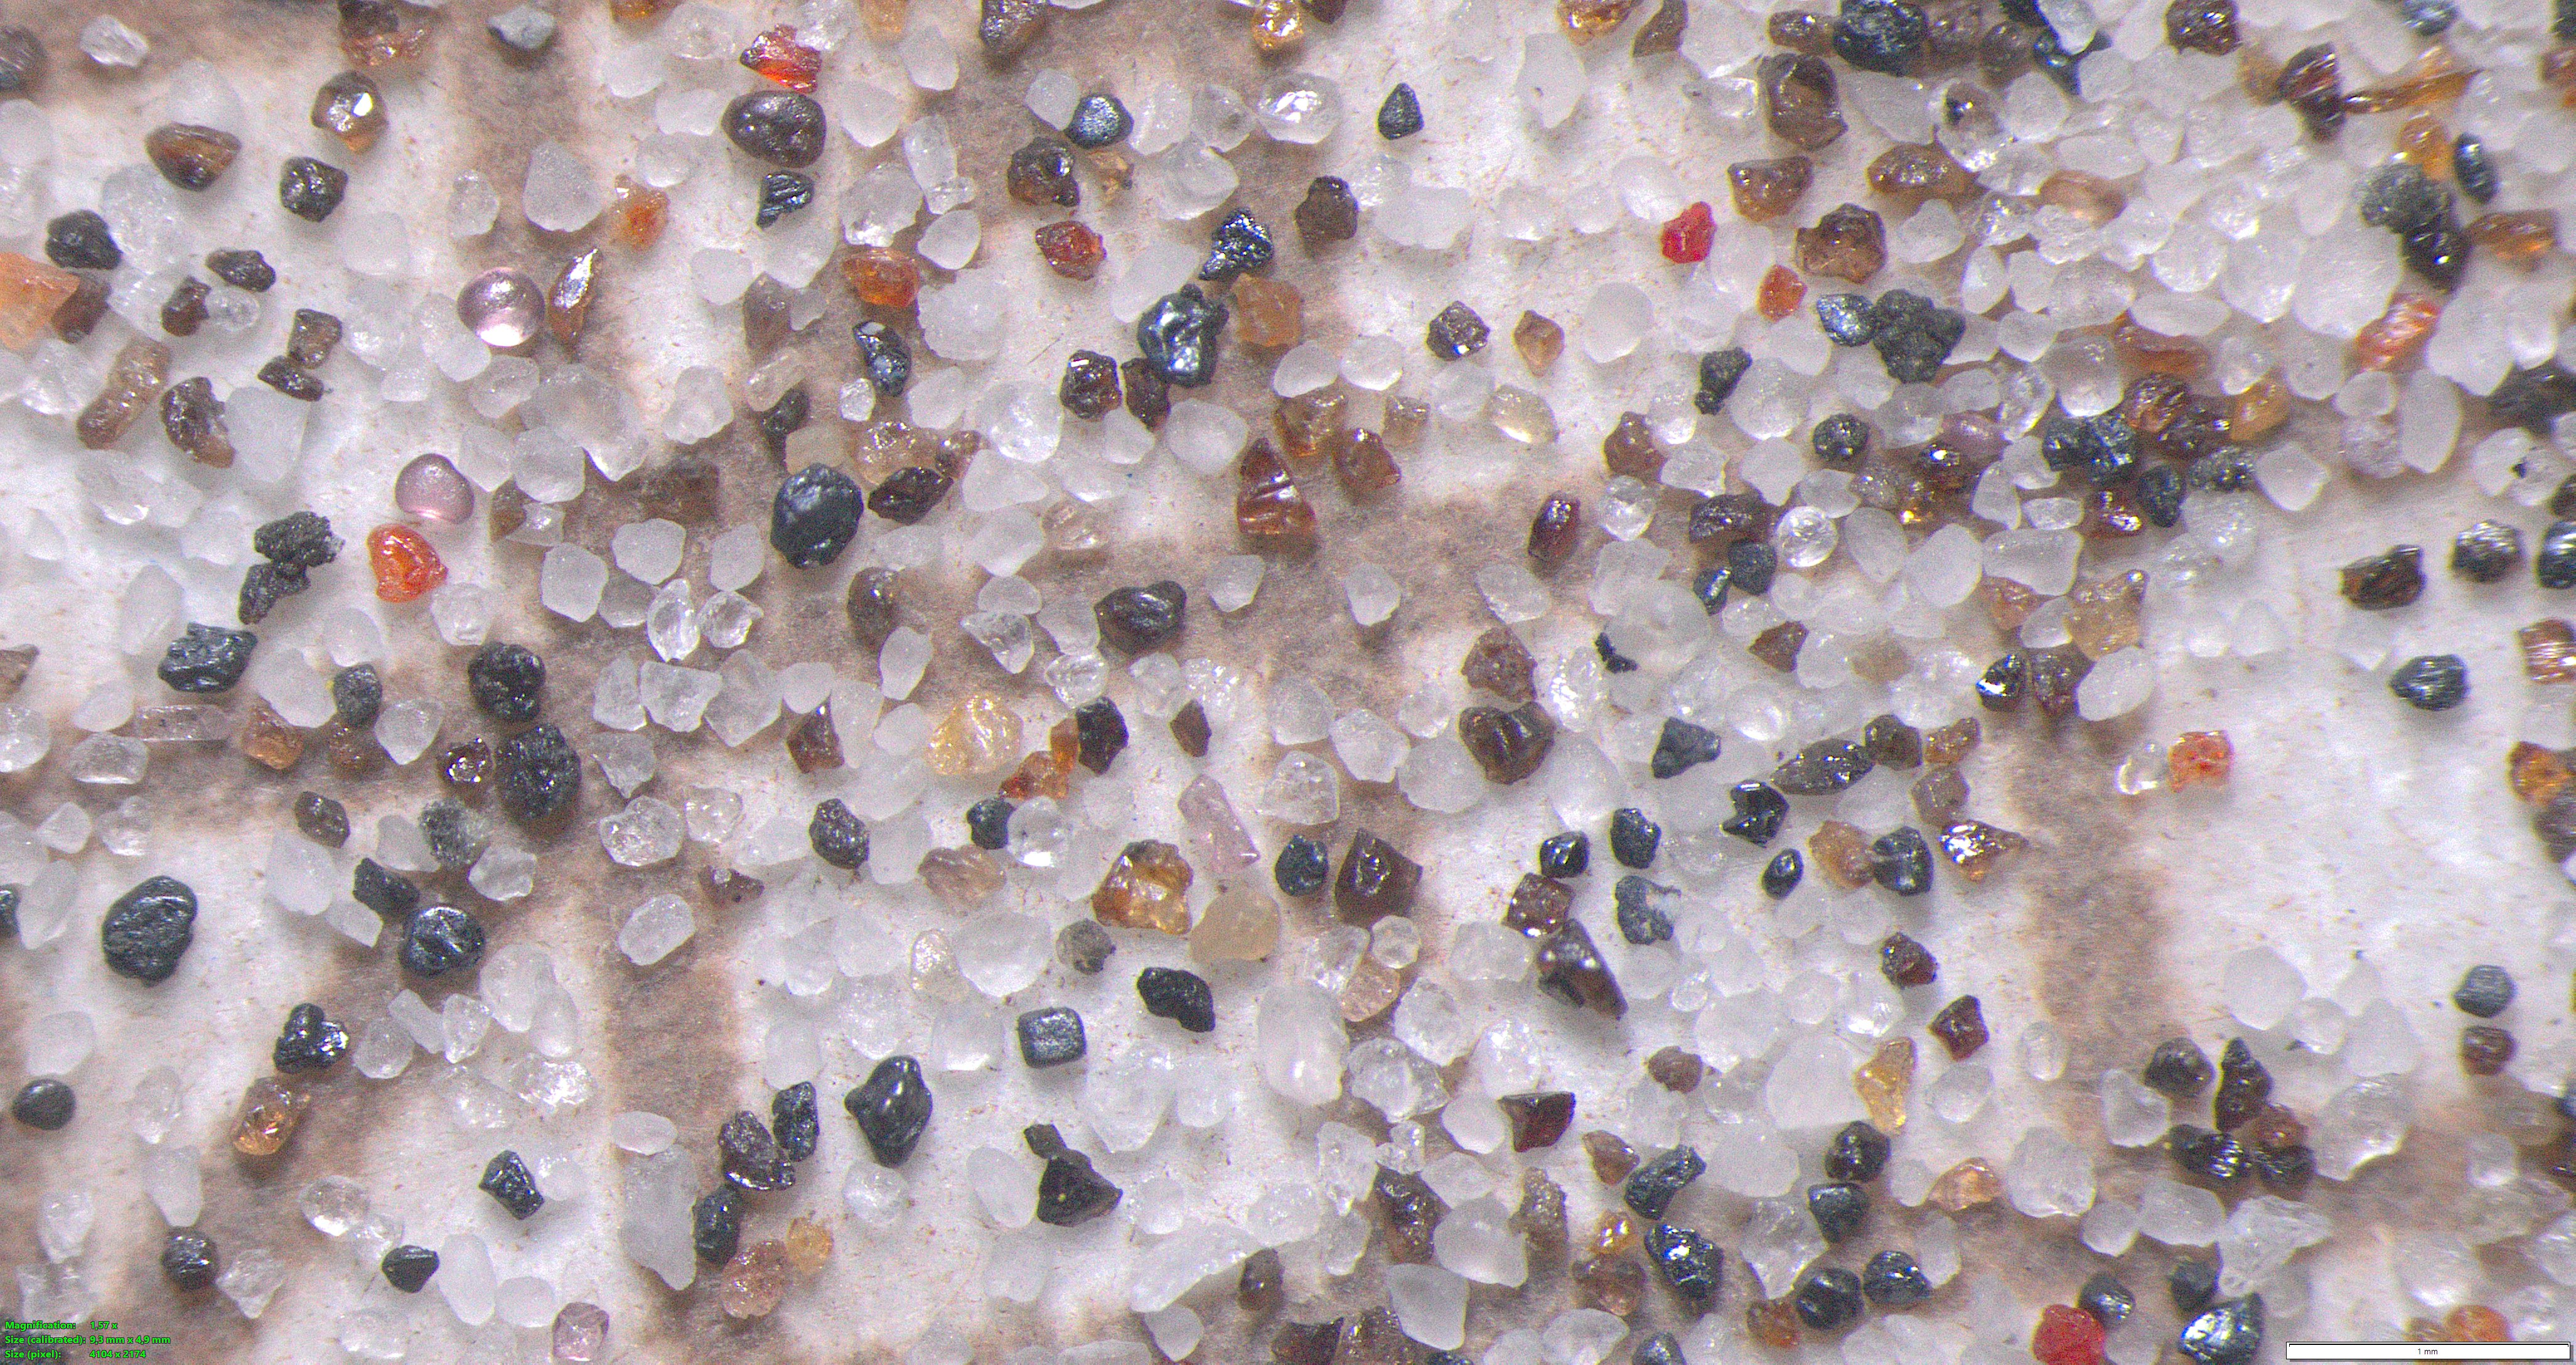
\includegraphics[width=\textwidth]{figure/sebeleumResize.jpg}
        \caption{Citra Awal tanpa \textit{Gaussian Noise}}
        \label{fig:3.GaussianAwal}
    \end{subfigure}
    \hfill
    \begin{subfigure}[b]{0.475\textwidth}
        \centering
        \includegraphics[width=\textwidth]{figure/hasilGaussianNoise.jpg}
        \caption{Hasil \textit{Gaussian Noise} dengan variansi 0{,}2}
        \label{fig:3.HasilGaussianNoise}
    \end{subfigure}

	\caption{Hasil \textit{Gaussian Noise} Data}
    \label{fig:3.HasilGaussianNoiseData}
\end{figure}

\subsubsection{\textit{Normalization}}
Pada tahapan ini, data citra mikroskop diolah dengan menerapkan teknik \textit{normalization} yang menyesuaikan rentang nilai piksel citra agar berada dalam skala tertentu, biasanya antara 0 hingga 1. Teknik ini digunakan untuk memastikan bahwa semua fitur pada citra memiliki kontribusi yang seimbang selama proses pelatihan model. Dengan melakukan \textit{normalization}, model dapat belajar lebih efektif karena perbedaan skala nilai piksel tidak akan memengaruhi proses pembelajaran.  \par

\begin{table}[h!]
\centering
\caption{Contoh piksel sebelum dinormalisasi}
\renewcommand{\arraystretch}{1.2} % Mengatur jarak antar baris
\setlength{\tabcolsep}{10pt} % Mengatur jarak antar kolom
\label{table:3.contoh-normalization}
\begin{tabular}{|c|c|c|c|c|}
\hline
\textbf{(i,j)} & \textbf{$(0,j)$} & \textbf{$(1,j)$} & \textbf{$(2,j)$} & \textbf{$(3,j)$} \\ \hline
$(i,0)$ & 123 & 45 & 200 & 89 \\ \hline
$(i,1)$ & 15  & 255 & 87 & 142 \\ \hline
$(i,2)$ & 64  & 31 & 219 & 176 \\ \hline
$(i,3)$ & 92  & 8 & 73 & 240 \\ \hline
\end{tabular}
\end{table}

Sebagai contoh, nilai piksel sebesar $X = 123$ yang terletak pada posisi baris ke-1 dan kolom ke-1 (indeks [0,0]) pada Tabel \ref{table:3.contoh-normalization} digunakan untuk perhitungan normalisasi. Berdasarkan Persamaan \ref{eq:2.normalization}, dengan $X_{min} = 0$ dan $X_{max} = 255$. Maka nilai piksel setelah dilakukan normalisasi ($X_{normal}$) dapat dihitung sebagai berikut: 

\begin{align*}
    X_{normal} &= \frac{X - X_{min}}{X_{max} - X_{min}} \\[0.5em]
    X_{normal} &= \frac{123 - 0}{255 - 0} \\[0.5em]
    X_{normal} &= \frac{123}{255} \\[0.5em]
    X_{normal} &= 0{,}482 \\[0.5em]
\end{align*}

Dengan demikian, nilai piksel pada indeks [0,0] sebesar $123$ setelah dilakukan normalisasi menjadi $0{,}482$, yang menunjukkan bahwa intensitas piksel tersebut telah diskalakan ke dalam rentang 0--1 sehingga siap digunakan dalam proses pelatihan model.

\begin{table}[h!]
\centering
\caption{Hasil piksel sebelum di normalisasii}
\renewcommand{\arraystretch}{1.2} % Mengatur jarak antar baris
\setlength{\tabcolsep}{10pt} % Mengatur jarak antar kolom
\label{table:3.Hasil-normalization}
\begin{tabular}{|c|c|c|c|c|}
\hline
\textbf{(i,j)} & \textbf{$(0,j)$} & \textbf{$(1,j)$} & \textbf{$(2,j)$} & \textbf{$(3,j)$} \\ \hline
$(i,0)$ & 0{,}482 & 0{,}176 & 0{,}784 & 0{,}349 \\ \hline
$(i,1)$ & 0{,}059 & 1{,}000 & 0{,}341 & 0{,}557 \\ \hline
$(i,2)$ & 0{,}251 & 0{,}122 & 0{,}859 & 0{,}690 \\ \hline
$(i,3)$ & 0{,}361 & 0{,}031 & 0{,}286 & 0{,}941 \\ \hline
\end{tabular}
\end{table}


\subsection{Pengembangan Model} \label{III.LangkahPengembanganModel}
Pada penelitian ini, alur pengembangan model yang digunakan dalam identifikasi mineral kasiterit pada citra mikroskop menggunakan \textit{Mask} R-CNN ditunjukkan pada Gambar \ref{fig:3.AlurPengembanganModel} berikut.\par

\begin{figure}[H] % Kalau menggunakan H, posisi gambar akan tepat dibawah teks
    \centering
    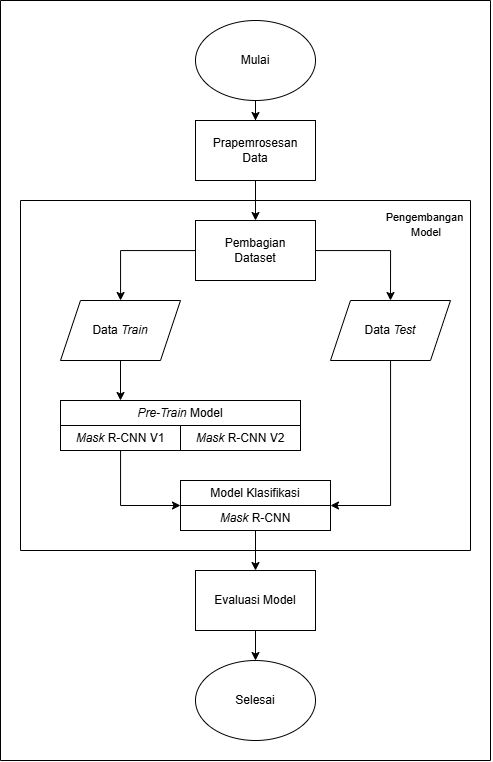
\includegraphics[width=0.73\textwidth]{figure/pengembanganModelfinal.png}
    \caption{Alur Pengembangan Model}
    \label{fig:3.AlurPengembanganModel}
\end{figure}

\subsubsection{Pembagian Data}
Pada tahapan ini, dataset yang telah melalui proses prapemrosesan dibagi menjadi data latih (\textit{training}) dan data validasi (\textit{validation}) menggunakan metode \textit{k-fold cross validation} dengan nilai $K=5$. Metode ini membagi dataset menjadi lima bagian (\textit{fold}) yang seimbang, di mana setiap \textit{fold} secara bergantian berperan sebagai data uji, sementara empat \textit{fold} lainnya digunakan untuk pelatihan. Dengan rasio pembagian 80:20 pada setiap iterasi, yaitu 80\% data digunakan untuk pelatihan dan 20\% data digunakan untuk pengujian, sehingga seluruh data memperoleh kesempatan untuk menjadi data uji setidaknya satu kali. \par

\subsubsection{Pelatihan Model}
Pada tahap ini, arsitektur \textit{Mask} R-CNN dilatih menggunakan data latih yang telah disiapkan sebelumnya. Penelitian terdahulu dengan topik serupa telah berhasil mengidentifikasi konfigurasi arsitektur yang efektif untuk tugas segmentasi objek mineral \cite{mineralogiMaskRCNNSolo} \cite{OreSegmentation2} \cite{unet}. Penelitian ini menggunakan dua \textit{Model Pre-trained} dari arsitektur \textit{Mask} R-CNN, yaitu dengan \textit{backbone} ResNet50 FPN versi V1 dan versi V2. Versi V2 tidak mengubah struktur arsitektur inti dari V1, tetapi meningkatkan performa melalui proses pelatihan ulang yang lebih mutakhir, meliputi penerapan augmentasi skala besar (\textit{Large Scale Jittering}), penggunaan normalisasi yang lebih stabil, penerapan regularisasi \textit{DropPath}, serta pemanfaatan \textit{optimizer AdamW} \cite{maskrcnnv2}. Strategi pelatihan yang lebih modern tersebut menghasilkan bobot \textit{pre-trained} yang lebih representatif dan akurat, dengan nilai \textit{mask} $mAP$ sebesar 41{,}8 pada V2, lebih tinggi dibandingkan V1 yang memperoleh 34{,}6 \cite{pytorchWebsite}.

Kedua arsitektur tersebut diuji pada dua bentuk model, yaitu model \textit{standar} dan model \textit{amodal}. Model \textit{standar} menggunakan \textit{mask head} konvensional yang hanya memprediksi bagian objek yang terlihat (\textit{visible mask}), sedangkan model \textit{amodal} dilengkapi dengan cabang jaringan tambahan (\textit{amodal mask head}) yang dirancang khusus untuk merekonstruksi bentuk utuh objek meskipun sebagian tertutup oleh objek lain (oklusi). 

\begin{figure}[H]
    \centering
    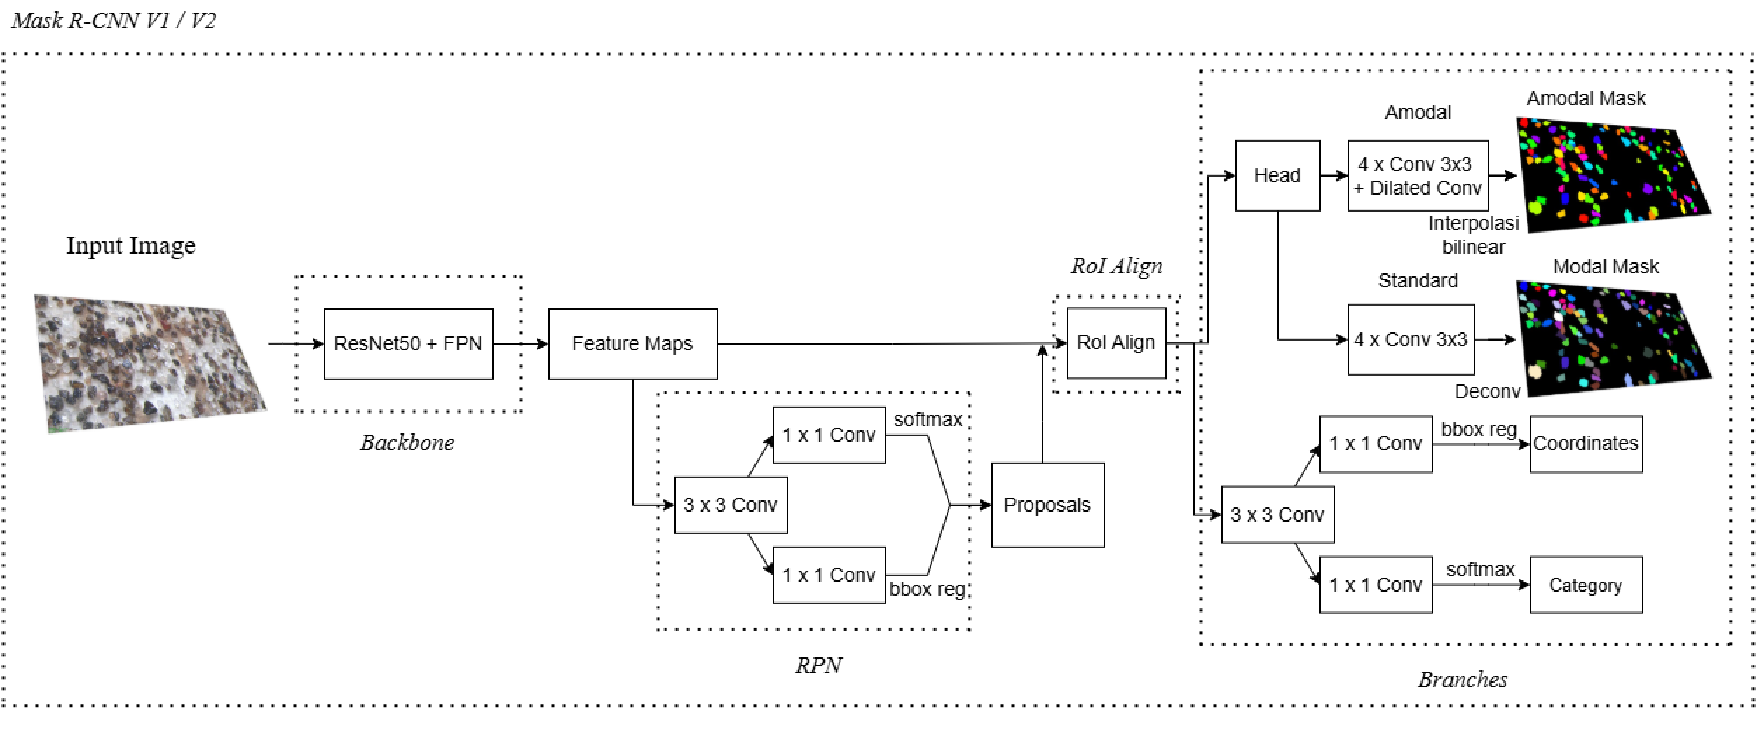
\includegraphics[page=1, width=1\textwidth]{doc/arsitektur ammodal.drawio2.pdf}
    \caption{Arsitektur \textit{Mask} R-CNN dengan cabang \textit{Amodal Instance Segmentation}}
    \label{fig:amodal-architecture}
\end{figure}

Sebagaimana ditunjukkan pada Gambar \ref{fig:amodal-architecture}, cabang \textit{amodal mask head} memiliki struktur arsitektur yang berbeda dibandingkan dengan \textit{modal mask head} standar. Pada cabang modal, arsitektur yang digunakan mengikuti struktur konvensional yang terdiri dari tumpukan lapisan konvolusi dan dilanjutkan dengan lapisan dekonvolusi untuk proses \textit{upsampling} \cite{MaskRcnnIEEE11}. Sementara itu, cabang amodal mengintegrasikan empat lapisan konvolusi $3 \times 3$ dengan lapisan \textit{dilated convolution}. Penerapan \textit{dilated convolution} bertujuan untuk memperluas \textit{receptive field} secara eksponensial tanpa mengorbankan resolusi spasial, sehingga mampu menangkap informasi konteks global pada berbagai skala \cite{dilatedConv}. Hal ini krusial bagi model dalam memprediksi kelanjutan struktur butiran mineral kasiterit yang teroklusi. Selanjutnya, lapisan \textit{upsample} berbasis interpolasi bilinear diterapkan untuk meningkatkan resolusi \textit{mask} secara halus guna menjaga konsistensi bentuk dan kontinuitas spasial objek, diikuti oleh lapisan konvolusi $1 \times 1$ untuk menghasilkan probabilitas piksel pada setiap lokasi \textit{mask amodal}. Melalui kombinasi komponen tersebut, model mampu merekonstruksi bentuk utuh mineral kasiterit meskipun sebagian areanya tertutup oleh butiran lain, yang pada akhirnya meningkatkan akurasi identifikasi pada kondisi oklusi dalam citra mikroskop. \par

Selain variasi model, kedua arsitektur juga dikombinasikan dengan dua algoritma optimasi berbeda, yaitu \textit{Stochastic Gradient Descent} (SGD) dan \textit{Adam}. Kombinasi antara variasi model dan algoritma optimasi tersebut menghasilkan delapan konfigurasi pelatihan sebagaimana ditunjukkan pada Tabel~\ref{table:3.konfigurasi-model}.
 
\begin{longtable}{|>{\centering\arraybackslash}p{0.25\textwidth}|>{\centering\arraybackslash}p{0.25\textwidth}|>{\centering\arraybackslash}p{0.25\textwidth}|} % Longtable berguna agar tabel dapat terpotong di halaman baru
    \caption{Variasi konfigurasi pelatihan}
        \label{table:3.konfigurasi-model}\\
        \hline
        \textbf{\textit{Model Pre-trained}} & \textbf{\textit{Model}} & \textbf{\textit{Optimizer}} \\
        \hline
        \endfirsthead % Header tabel untuk halaman pertama
        \hline
        \textbf{\textit{Model Pre-trained}} & \textbf{\textit{Model}} & \textbf{\textit{Optimizer}} \\
        \hline
        \endhead % Header tabel untuk halaman selanjutnya (repeat header row)
        \multirow{4}{*}{\shortstack{\textit{Mask} R-CNN \\ResNet50 FPN V1}} & \multirow{2}{*}{\textit{Amodal}} & SGD \\
        \cline{3-3}
         & & \textit{Adam} \\
        \cline{2-3}
         & \multirow{2}{*}{\textit{Standar}} & SGD \\
        \cline{3-3}
         & & \textit{Adam} \\
        \hline
        \multirow{4}{*}{\shortstack{\textit{Mask} R-CNN \\ResNet50 FPN V2}} & \multirow{2}{*}{\textit{Amodal}} & SGD \\
        \cline{3-3}
         & & \textit{Adam} \\
        \cline{2-3}
         & \multirow{2}{*}{\textit{Standar}} & SGD \\
        \cline{3-3}
         & & \textit{Adam} \\
        \hline
\end{longtable}

\subsection{Evaluasi Model} \label{III.LangkahEvaluasiModel}
Pada tahap evaluasi, setiap variasi konfigurasi pelatihan pada model \textit{Mask} R-CNN diuji untuk menilai pengaruhnya terhadap kinerja model. Evaluasi dilakukan menggunakan data validasi yang telah dipisahkan sebelumnya agar hasil yang diperoleh bersifat objektif dan bebas dari bias data latih. Kinerja model diukur berdasarkan dua metrik utama, yaitu \textit{Average Precision} (AP) dan \textit{Intersection over Union} (IoU), yang digunakan untuk menilai tingkat akurasi deteksi serta kualitas segmentasi objek. Metrik AP dihitung pada tiga \textit{threshold} yang berbeda, yaitu \APfifty, \APseventyfive, dan \APrangefifty, untuk mengukur performa model pada tingkat keketatan deteksi yang bervariasi. Begitu pula dengan IoU, yang dihitung pada \IoUfifty, \IoUseventyfive, dan \IoUrangefifty guna mengevaluasi kualitas tumpang tindih antara prediksi dan \textit{ground truth} pada berbagai tingkat presisi. Evaluasi ini juga mempertimbangkan penerapan teknik \textit{amodal instance segmentation} untuk menguji kemampuan model mengenali objek yang saling menutupi pada citra uji. Hasil evaluasi dari setiap konfigurasi kemudian dibandingkan untuk menentukan kombinasi konfigurasi pelatihan yang memberikan performa terbaik. \par


\subsection{Hasil dan Pembahasan} \label{III.LangkahHasilDanPembahasan}
Pada tahap ini, setelah model \textit{Mask} R-CNN selesai dilakukan evaluasi, diperoleh hasil perbandingan dari setiap variasi konfigurasi pelatihan yang telah diuji. Hasil performa dari setiap variasi konfigurasi pelatihan akan dibandingkan untuk mengetahui model mana yang paling optimal dalam melakukan identifikasi mineral kasiterit pada citra mikroskop berdasarkan metrik \textit{Average Precision} (AP) dan \textit{Intersection over Union} (IoU) termasuk pada penerapan teknik \textit{amodal instance segmentation} untuk mendeteksi butiran yang saling menutupi. Berdasarkan hasil analisis, akan diperoleh kesimpulan mengenai efektivitas masing-masing variasi konfigurasi pelatihan dalam melakukan identifikasi mineral kasiterit. Selain itu, kesimpulan juga dapat menjadi dasar untuk penelitian atau pengembangan selanjutnya. \par

\section{Alat dan Bahan Tugas Akhir} \label{III.Alat dan Bahan}
Alat dan Bahan yang digunakan dalam penelitian tugas akhir ini adalah sebagai berikut: \par

\subsection{Alat} \label{III.Alat}
Alat yang digunakan untuk melakukan penelitian tugas akhir ini adalah sebagai berikut: \par
\begin{enumerate}[noitemsep]
	\item Laptop ASUS TUF FX517ZC dengan sistem operasi Windows 11 Home 64-bit, RAM 16 GB DDR5, prosesor Intel® Core™ i7-12650H, kartu grafis NVIDIA® GeForce RTX™ 3050 4GB GDDR6.
	\item Visual Studio Code versi 1.109.0 dan Antigravity versi 1.107.0 untuk melakukan pengembangan kode program dan penulisan dokumentasi.
	\item Github untuk menyimpan kode program, dataset dan dokumentasi secara daring.
	\item Notion untuk mencatat revisi dan informasi, sekaligus untuk manajemen proyek.
	\item Labelme with SAM \cite{Wada_Labelme_Image_Polygonal} untuk melakukan segmentasi data citra mikroskop.
	\item Runpod untuk melakukan pelatihan model \textit{Mask} R-CNN menggunakan GPU RTX PRO 6000.
\end{enumerate}

\subsection{Bahan} \label{III.Bahan}
Bahan yang digunakan pada penelitian ini adalah dataset citra mikroskop mineral kasiterit yang bersumber dari Laboratorium Eksplorasi PT. Timah Tbk yang berlokasi di Kota Pangkalpinang, Bangka Belitung \cite{PTTimahWebsite}.\par

\section{Metode Pengembangan} \label{III.Metode}
Pada penelitian ini, metode pengembangan yang digunakan adalah \textit{Mask} R-CNN untuk mengidentifikasi dan dapat melakukan segmentasi mineral kasiterit pada citra mikroskop dengan membandingkan beberapa variasi konfigurasi pelatihan serta menerapkan teknik \textit{amodal instance segmentation} agar model dapat mengenali bentuk utuh butiran mineral yang saling menutupi pada citra mikroskop. 

\section{Ilustrasi Perhitungan Metode} \label{III.Ilustrasi}
Berikut adalah ilustrasi perhitungan yang dilakukan pada penelitian ini. \par

\subsection{\textit{Loss Function Mask} R-CNN}
Bagian ini menjelaskan secara rinci proses perhitungan fungsi kerugian (\textit{loss function}) pada arsitektur \textit{Mask R-CNN}, yang terdiri dari tiga komponen utama: \textit{Classification Loss} ($L_{\text{cls}}$), \textit{Bounding Box Regression Loss} ($L_{\text{box}}$), dan \textit{Mask Loss} ($L_{\text{mask}}$). Ketiga komponen ini bekerja bersama untuk mengoptimalkan performa deteksi dan segmentasi objek pada citra. 
Fungsi kerugian total ($L$) pada \textit{Mask R-CNN} dapat dihitung dengan menjumlahkan ketiga komponen tersebut, seperti yang ditunjukkan pada \ref{eq:2.maskrcnn}. \par

% \begin{align*}
%     L &= L_{\text{cls}} + L_{\text{box}} + L_{\text{mask}} \\[0.5em]
% \end{align*}

Sebagai ilustrasi penerapan perhitungan fungsi kerugian secara keseluruhan, digunakan contoh data yang terdiri dari hasil perhitungan ketiga komponen loss, yaitu $L_{\text{cls}} = 0{,}27002$, $L_{\text{box}} = 0{,}0023$, dan $L_{\text{mask}} = 0{,}1923$. Dengan memasukkan nilai-nilai tersebut ke dalam rumus total loss pada \textit{Mask} R-CNN, diperoleh perhitungan akhir sebagai berikut: \par

\begin{align*}
    L &= L_{\text{cls}} + L_{\text{box}} + L_{\text{mask}} \\[0.5em]
    L &= 0{,}27002 + 0{,}0023 + 0{,}1923 \\[0.5em]
    L &= 0{,}46462
\end{align*}

\subsubsection{Perhitungan $L_{\text{cls}}$ \textit{(Classification Loss)}}

Fungsi kerugian klasifikasi digunakan untuk mengukur seberapa baik model dalam memprediksi label kelas untuk setiap \textit{Region of Interest} (RoI). Pada Mask R-CNN, fungsi ini biasanya menggunakan \textit{binary cross-entropy loss} yang membandingkan nilai prediksi ($p_i$) dengan label sebenarnya ($p_i^*$) menggunakan logaritma natural yang di definisikan sebagai $\log$, seperti yang ditunjukkan pada \ref{eq:2.cls_loss}.  \par

% \begin{align*}
%     L_{\text{cls}} &= \frac{1}{N_{\text{cls}}} \sum_i \big(-p_i^* \log p_i - (1 - p_i^*) \log (1 - p_i)\big) \\[0.5em]
% \end{align*}

Tabel berikut menunjukkan data contoh lima RoI yang digunakan dalam ilustrasi perhitungan ini, masing-masing memiliki nilai prediksi ($p_i$), label kebenaran ($p_i^*$), dan ukuran mask yang seragam ($4\times4$), seperti yang ditunjukkan pada Tabel \ref{table:3.contoh-data-roi-loss} berikut. \par

\begin{table}[H]
\centering
\caption{Contoh Data RoI untuk Ilustrasi Perhitungan \textit{Classification Loss} R-CNN}
\renewcommand{\arraystretch}{1.3}
\label{table:3.contoh-data-roi-loss}
\begin{tabular}{|c|c|c|>{\centering\arraybackslash}m{2.2cm}|}
\hline
\textbf{RoI} & \textbf{$p_i$ (prediksi)} & \textbf{$p_i^*$ (label)} & \textbf{Ukuran Mask} \\ 
\hline
1 & 0,80 & 1 & $4 \times 4$ \\ 
\hline
2 & 0,60 & 1 & $4 \times 4$ \\ 
\hline
3 & 0,20 & 0 & $4 \times 4$ \\ 
\hline
4 & 0,75 & 1 & $4 \times 4$ \\ 
\hline
5 & 0,10 & 0 & $4 \times 4$ \\ 
\hline
\end{tabular}
\end{table}

Jumlah total RoI yang digunakan adalah lima, sehingga $N_{\text{cls}} = 5$. Perhitungan dilakukan dengan memasukkan nilai-nilai prediksi dan label ke dalam rumus \textit{cross-entropy loss} untuk tiap RoI. Dalam perhitungan ini, kita akan menggunakan data $p_i = 0{,}8$ dan $p_i^* = 1$ sebagai contoh untuk RoI pertama. \par 

\begin{align*}
    L_{\text{cls}} &= \frac{1}{N_{\text{cls}}} \sum_i \big(-p_i^* \log p_i - (1 - p_i^*) \log (1 - p_i)\big) \\[0.5em]
     &= \frac{1}{5} \sum_{i=1}^{5} \big(-1 \cdot \log 0{,}8 - (1 - 1) \log (1 - 0{,}8)\big) \\[0.5em]
     &= \frac{1}{5} \sum_{i=1}^{5} \big(-1 \cdot \log 0{,}8 - 0 \cdot \log (1 - 0{,}8)\big) \\[0.5em]
     &= \frac{1}{5} \sum_{i=1}^{5} \big(-\log 0{,}8 \big) \\[0.5em]
     &= \frac{1}{5} \sum_{i=1}^{5} 0{,}2231 \\[0.5em]
     &= 0{,}2231 \\[0.5em]
\end{align*}

Berikut hasil lengkap perhitungan per-RoI untuk $L_{\text{cls}}$.

\begin{table}[H]
\centering
\caption{Perhitungan $L_{\text{cls}}$ (klasifikasi)}
\renewcommand{\arraystretch}{1.3}
\label{table:3.loss-cls}
\begin{tabular}{|c|c|c|>{\centering\arraybackslash}m{3.7cm}|c|}
\hline
\textbf{RoI} & \textbf{$p_i$ (prediksi)} & \textbf{$p_i^*$ (label)} & \textbf{Rumus terapan} & \textbf{Hasil} \\ 
\hline
1 & 0,80 & 1 & $-\log 0{,}8$ & 0{,}2231 \\ 
\hline
2 & 0,60 & 1 & $-\log 0{,}6$ & 0{,}5108 \\ 
\hline
3 & 0,20 & 0 & $-\log (1-0{,}2) = -\log 0{,}8$ & 0{,}2231 \\ 
\hline
4 & 0,75 & 1 & $-\log 0{,}75$ & 0{,}2877 \\ 
\hline
5 & 0,10 & 0 & $-\log (1-0{,}1) = -\log 0{,}9$ & 0{,}1054 \\ 
\hline
\end{tabular}
\end{table}

Dengan menjumlahkan seluruh hasil dan membaginya dengan jumlah RoI, diperoleh nilai rata-rata $L_{\text{cls}}$ sebesar:

\begin{align*}
    L_{\text{cls}} &= \frac{0{,}2231 + 0{,}5108 + 0{,}2231 + 0{,}2877 + 0{,}1054}{5} \\[0.5em]
     &= \frac{1{,}3501}{5} \\[0.5em]
     &= 0{,}27002
\end{align*}

\subsubsection{Perhitungan $L_{\text{box}}$ \textit{(Bounding Box Regression Loss)}}
Bagian ini menghitung kesalahan antara koordinat prediksi kotak pembatas ($t_i$) dan nilai kebenarannya ($t_i^*$). Komponen ini menggunakan fungsi $L_1^{\text{smooth}}$, yang merupakan versi halus dari \textit{L1 loss} untuk menghindari perubahan gradien mendadak, seperti yang ditunjukkan pada \ref{eq:2.box_loss}.

% \begin{align*}
%     L_{\text{box}} &= \frac{\lambda}{N_{\text{box}}} \sum_i p_i^* \cdot L_1^{\text{smooth}}(t_i - t_i^*) \\[0.5em]
% \end{align*}

Data berikut menunjukkan tiga RoI dengan label positif ($p_i^* = 1$), yang digunakan untuk menghitung $L_{\text{box}}$ sebanyak 3 RoI, seperti yang ditunjukkan pada Tabel \ref{table:3.contoh-data-box-loss-pos} berikut.

\begin{table}[H]
\centering
\caption{Contoh Data RoI (hanya label = 1) dengan $t_i$, $t_i^*$ dan hasil bbox ($t_i - t_i^*$)}
\renewcommand{\arraystretch}{1.3}
\label{table:3.contoh-data-box-loss-pos}
\begin{tabular}{|c|c|>{\centering\arraybackslash}m{2.4cm}|>{\centering\arraybackslash}m{2.6cm}|}
\hline
\textbf{RoI} & \textbf{$p_i^*$} & \textbf{$t_i$ (prediksi)} & \textbf{$t_i^*$ (ground-truth)} \\ 
\hline
1 & 1 & [0{,}55; \,0{,}45; \newline\,0{,}62; \,0{,}52] & [0{,}45; \,0{,}50; \newline\,0{,}60; \,0{,}55] \\ 
\hline
2 & 1 & [0{,}68; \,-0{,}22; \newline\,0{,}55; \,0{,}21] & [0{,}60; \,-0{,}20; \newline\,0{,}50; \,0{,}20] \\ 
\hline
4 & 1 & [0{,}55; \,0{,}44; \newline\,-0{,}28; \,-0{,}16] & [0{,}50; \,0{,}40; \newline\,-0{,}25; \,-0{,}15] \\ 
\hline
\end{tabular}
\end{table}

Perhitungan selisih $t_i - t_i^*$ menghasilkan vektor $d$, yang selanjutnya digunakan dalam fungsi $L_1^{\text{smooth}}$. Karena semua komponen memiliki nilai $|d| < 1$, maka digunakan rumus $\frac{1}{2}d^2$ untuk setiap elemen. Sebagai contoh perhitungan untuk RoI pertama menggunakan  ${t_i} = [0{,}55; \,0{,}45; \,0{,}62; \,0{,}52]$ dan ${t_i^*} = [0{,}45; \,0{,}50; \,0{,}60; \,0{,}55]${,}

\begin{align*}
    {t_i - t_i^*} &= [0{,}55; \,0{,}45; \,0{,}62; \,0{,}52] - [0{,}45; \,0{,}50; \,0{,}60; \,0{,}55] \\[0.5em]
    {t_i - t_i^*} &= [0{,}10; \,-0{,}05; \,0{,}02; \,-0{,}03] \\[0.5em]
\end{align*}

Dari hasil selisih ($t_i - t_i^*$) atau $d$ pada perhitungan di atas, dapat dilihat bahwa semua nilai $d$ memenuhi kondisi $|d| < 1$. Oleh karena itu, fungsi $L_1^{\text{smooth}}(t_i - t_i^*)$ yang digunakan adalah $\frac{1}{2}d^2$ untuk setiap komponen vektor $d$. Sebagai contoh, perhitungan dilakukan untuk komponen pertama vektor $d$ yaitu $d[0] = 0{,}10$ sebagai berikut:

% \begin{align*}
%     {t_i - t_i^*} &= d = [0.10; \,-0.05; \,0.02; \,-0.03] \\[0.5em]
% \end{align*}

\begin{align*}
    d[0] &= 0{,}10 = |0{,}10| = \frac{1}{2}(0{,}10)^2 = 0{,}0050 \\
    % d[1] &= -0.05 = |0.05| = \frac{1}{2}(0.05)^2 = 0.00125 \\[0.5em]
    % d[2] &= 0.02 = |0.02| = \frac{1}{2}(0.02)^2 = 0.0002 \\[0.5em]
    % d[3] &= -0.03 = |0.03| = \frac{1}{2}(0.03)^2 = 0.00045 \\[0.5em]
\end{align*}

Setelah menghitung nilai smooth $L_1$ untuk setiap komponen vektor $d$, diperoleh empat nilai yaitu $0{,}0050$; $0{,}00125$; $0{,}0002$; dan $0{,}00045$. Selanjutnya, hasil dari semua komponen tersebut dijumlahkan untuk memperoleh total nilai $L_1^{\text{smooth}}(t_i - t_i^*)$ untuk RoI pertama. Perhitungan dilakukan sebagai berikut:

\begin{align*}
    L_1^{\text{smooth}}(t_i - t_i^*) &= 0{,}0050 + 0{,}00125 + 0{,}0002 + 0{,}00045 \\[0.5em]
     &= 0{,}0069 \\[0.5em]
     &= 0{,}0050 + 0{,}00125 + 0{,}0002 + 0{,}00045 \\[0.5em]
     &= 0{,}0069 \\[0.5em]
\end{align*}

Dengan cara yang sama, perhitungan $L_1^{\text{smooth}}(t_i - t_i^*)$ dilakukan untuk RoI kedua dan keempat, menghasilkan nilai 0{,}0035 dan 0{,}0018 secara berurutan. Selanjutnya, nilai-nilai ini digunakan untuk menghitung total $L_{\text{box}}$ dengan memasukkan nilai-nilai tersebut ke dalam rumus utama. \\
\begin{align*}
    L_{\text{box}} &= \frac{\lambda}{N_{\text{box}}} \sum_i p_i^* \cdot L_1^{\text{smooth}}(t_i - t_i^*) \\[0.5em]
     &= \frac{1}{3} \sum_{i=1}^{3} 1 \cdot 0{,}0069 \\[0.5em]
     &= \frac{1}{3} \cdot 0{,}0069 \\[0.5em]
     &= 0{,}0023 \\[0.5em]
\end{align*}

Tabel \ref{table:3.hasil-data-box-loss-pos} berikut menunjukkan hasil perhitungan $L_{\text{box}}$ untuk setiap RoI dengan label positif ($p_i^* = 1$). Pada tabel tersebut dapat dilihat selisih antara prediksi dan ground truth ($t_i - t_i^*$), nilai $L_1^{\text{smooth}}$ untuk masing-masing RoI, serta kontribusi setiap RoI terhadap total $L_{\text{box}}$.

\begin{table}[H]
\centering
\caption{Hasil Akhir Perhitungan $L_{\text{box}}$}
\renewcommand{\arraystretch}{1.3}
\label{table:3.hasil-data-box-loss-pos}
\begin{tabular}{|c|>{\centering\arraybackslash}m{1.9cm}|>{\centering\arraybackslash}m{1.9cm}|>{\centering\arraybackslash}m{1.9cm}|>{\centering\arraybackslash}m{1.4cm}|c|}
\hline
\textbf{RoI} & \textbf{$t_i$} & \textbf{$t_i^*$} & \textbf{$t_i - t_i^*$ ($d$)} & \textbf{$L_1^{\text{smooth}}$} & \textbf{$L_{\text{box}}$} \\ 
\hline
1 & [0{,}55; \,0{,}45; \newline\,0{,}62; \,0{,}52] & [0{,}45; \,0{,}50; \newline\,0{,}60; \,0{,}55] & [0{,}10; \,-0{,}05; \newline\,0{,}02; \,-0{,}03] & 0{,}0069 & 0{,}0023 \\ 
\hline
2 & [0{,}68; \,-0{,}22; \newline\,0{,}55; \,0{,}21] & [0{,}60; \,-0{,}20; \newline\,0{,}50; \,0{,}20] & [0{,}08; \,-0{,}02; \newline\,0{,}05; \,0{,}01] & 0{,}0035 & 0{,}0012 \\ 
\hline
4 & [0{,}55; \,0{,}44; \newline\,-0{,}28; \,-0{,}16] & [0{,}50; \,0{,}40; \newline\,-0{,}25; \,-0{,}15] & [0{,}05; \,0{,}04; \newline\,-0{,}03; \,-0{,}01] & 0{,}0018 & 0{,}0006 \\ 
\hline
\end{tabular}
\end{table}

\subsubsection{Perhitungan $L_{\text{mask}}$ \textit{(Mask Loss)}}
Komponen ini berfungsi mengukur seberapa akurat model dalam menghasilkan segmentasi piksel objek dibandingkan dengan mask sebenarnya. Setiap piksel dihitung menggunakan \textit{binary cross-entropy} berdasarkan probabilitas prediksi $\hat{y}_{ij}$ dan label kebenaran $y_{ij}$, seperti yang ditunjukkan pada \ref{eq:2.maskloss}.

% \begin{align*}
% 	L_{\text{mask}} &= -\frac{1}{m^2}\sum_{1 \leq i,j \leq m}
% 	\Big[ y_{ij} \log \hat{y}^{k}_{ij} + (1 - y_{ij}) \log (1 - \hat{y}^{k}_{ij}) \Big] \\[0.5em]
% \end{align*}

Ukuran mask yang digunakan adalah $4 \times 4$, sehingga jumlah piksel total $m^2 = 16$. Berikut contoh representasi nilai label dan prediksi yang digunakan: \\

\begin{align*}
y_{ij} &=
\begin{bmatrix}
1 & 1 & 0 & 0 \\
1 & 1 & 0 & 0 \\
1 & 0 & 0 & 0 \\
0 & 0 & 0 & 0
\end{bmatrix}, \quad
\hat{y}_{ij} =
\begin{bmatrix}
0{,}9 & 0{,}8 & 0{,}2 & 0{,}1 \\
0{,}9 & 0{,}7 & 0{,}3 & 0{,}2 \\
0{,}8 & 0{,}4 & 0{,}1 & 0{,}1 \\
0{,}2 & 0{,}1 & 0{,}1 & 0{,}0
\end{bmatrix}
\\[0.5em]
\end{align*}

Untuk menghitung \textit{mask loss} secara detail, perhitungan dilakukan untuk setiap piksel pada mask yang berukuran $4 \times 4$. Setiap piksel diidentifikasi menggunakan index $(i,j)$ yang dimulai dari $(0,0)$ hingga $(3,3)$, di mana $i$ mewakili index baris dan $j$ mewakili index kolom. Perhitungan \textit{loss} untuk setiap piksel dilakukan dengan terlebih dahulu memecah rumus utama menjadi bentuk yang lebih sederhana, yaitu $\text{loss}_{ij}$. Dengan demikian, rumus \textit{mask loss} dapat ditulis ulang menjadi:

\begin{align*}
    L_{\text{mask}} &= \frac{1}{m^2}\sum_{1 \leq i,j \leq m} \text{loss}_{ij} \\[0.5em]
\end{align*}

Di mana nilai $\text{loss}_{ij}$ untuk setiap piksel pada mask dihitung secara terpisah menggunakan rumus di bawah ini yang menerapkan fungsi \textit{binary cross-entropy} untuk membandingkan nilai prediksi dengan nilai sebenarnya:

\begin{align*}
    % \\[0.5em]
	{\text{loss}_{ij}} &= -\Big[ y_{ij} \log \hat{y}^{k}_{ij} + (1 - y_{ij}) \log (1 - \hat{y}^{k}_{ij}) \Big] \\[0.5em]
\end{align*}

Sebagai contoh, perhitungan untuk piksel pertama dengan index $(0,0)$ dilakukan menggunakan nilai $y_{ij} = 1$ dan $\hat{y}_{ij} = 0{,}9$ sebagai berikut:

\begin{align*}
    % \\[0.5em]
	{\text{loss}_{ij}} &= -\Big[ y_{ij} \log \hat{y}^{k}_{ij} + (1 - y_{ij}) \log (1 - \hat{y}^{k}_{ij}) \Big] \\[0.5em]
	 &= -\Big[ 1 \cdot \log 0{,}9 + (1 - 1) \log (1 - 0{,}9) \Big] \\[0.5em]
	 &= -\Big[ 1 \cdot \log 0{,}9 + 0 \cdot \log (0{,}1) \Big] \\[0.5em]
	 &= -\Big[\log 0{,}9 \Big] \\[0.5em]
	 &= 0{,}1057\\[0.5em]
\end{align*}

Dengan cara yang sama, perhitungan dilakukan untuk setiap piksel pada seluruh index ($i = 0, 1, 2, 3$) menggunakan rumus yang telah ditetapkan. Adapun hasil perhitungan untuk salah satu indeks yaitu indeks 0, adalah sebagai berikut. \par

\textbf{Index 0 ($i = 0$)}
\begin{table}[H]
\centering
% \caption{data tabel Index 0 ($i = 0$)}
\renewcommand{\arraystretch}{1.3}
\label{table:3.data-index-0}
\begin{tabular}{|c|c|c|c|c|}
\hline
\textbf{(i,j)} & \textbf{$y_{ij}$} & \textbf{$\hat{y}_{ij}$} & \textbf{Bentuk Rumus} & \textbf{Hasil} \\
\hline
(0,0) & 1 & 0{,}9 & $-\log(0{,}9)$ & 0{,}1054 \\ \hline
(0,1) & 1 & 0{,}8 & $-\log(0{,}8)$ & 0{,}2231 \\ \hline
(0,2) & 0 & 0{,}2 & $-\log(1-0{,}2)=-\log(0{,}8)$ & 0{,}2231 \\ \hline
(0,3) & 0 & 0{,}1 & $-\log(1-0{,}1)=-\log(0{,}9)$ & 0{,}1054 \\
\hline
\end{tabular}
\end{table}

% \textbf{Index 1 ($i = 1$)}
% \begin{table}[H]
% \centering
% % \caption{data tabel Index 1 ($i = 1$)}
% \renewcommand{\arraystretch}{1.3}
% \label{table:3.data-index-1}
% \begin{tabular}{|c|c|c|c|c|}
% \hline
% \textbf{(i,j)} & \textbf{$y_{ij}$} & \textbf{$\hat{y}_{ij}$} & \textbf{Bentuk Rumus} & \textbf{Hasil} \\
% \hline
% (1,0) & 1 & 0.9 & $-\log(0.9)$ & 0.1054 \\ \hline
% (1,1) & 1 & 0.7 & $-\log(0.7)$ & 0.3567 \\ \hline
% (1,2) & 0 & 0.3 & $-\log(1-0.3)=-\log(0.7)$ & 0.3567 \\ \hline
% (1,3) & 0 & 0.2 & $-\log(1-0.2)=-\log(0.8)$ & 0.2231 \\
% \hline
% \end{tabular}
% \end{table}

% \textbf{Index 2 ($i = 2$)}
% \begin{table}[H]
% \centering
% % \caption{data tabel Index 2 ($i = 2$)}
% \renewcommand{\arraystretch}{1.3}
% \label{table:3.data-index-2}
% \begin{tabular}{|c|c|c|c|c|}
% \hline
% \textbf{(i,j)} & \textbf{$y_{ij}$} & \textbf{$\hat{y}_{ij}$} & \textbf{Bentuk Rumus} & \textbf{Hasil} \\
% \hline
% (2,0) & 1 & 0.8 & $-\log(0.8)$ & 0.2231 \\ \hline
% (2,1) & 0 & 0.4 & $-\log(1-0.4)=-\log(0.6)$ & 0.5108 \\ \hline
% (2,2) & 0 & 0.1 & $-\log(1-0.1)=-\log(0.9)$ & 0.1054 \\ \hline
% (2,3) & 0 & 0.1 & $-\log(1-0.1)=-\log(0.9)$ & 0.1054 \\
% \hline
% \end{tabular}
% \end{table}

% \textbf{Index 3 ($i = 3$)}
% \begin{table}[H]
% \centering
% % \caption{data tabel Index 3 ($i = 3$)}
% \renewcommand{\arraystretch}{1.3}
% \label{table:3.data-index-3}
% \begin{tabular}{|c|c|c|c|c|}
% \hline
% \textbf{(i,j)} & \textbf{$y_{ij}$} & \textbf{$\hat{y}_{ij}$} & \textbf{Bentuk Rumus} & \textbf{Hasil} \\
% \hline
% (3,0) & 0 & 0.2 & $-\log(1-0.2)=-\log(0.8)$ & 0.2231 \\ \hline
% (3,1) & 0 & 0.1 & $-\log(1-0.1)=-\log(0.9)$ & 0.1054 \\ \hline
% (3,2) & 0 & 0.1 & $-\log(1-0.1)=-\log(0.9)$ & 0.1054 \\ \hline
% (3,3) & 0 & 0.0 & $-\log(1-0.0)=-\log(1)=0$ & 0.0000 \\
% \hline
% \end{tabular}
% \end{table}

% di index (3,3), y = 0 dan ŷ = 0 → model yakin ini latar belakang, dan benar → loss = 0.

Setelah menghitung nilai $\text{loss}_{ij}$ untuk setiap piksel pada seluruh index, langkah selanjutnya adalah menjumlahkan hasil perhitungan per index. Penjumlahan ini dilakukan dengan menambahkan semua nilai $\text{loss}_{ij}$ pada setiap baris ($i = 0, 1, 2, 3$) untuk mendapatkan total \textit{loss} pada masing-masing index. Adapun hasil perhitungan untuk salah satu $\text{loss}_{ij}$, yaitu $\text{loss}_{0j}$ pada index 0, adalah sebagai berikut. \par

\begin{align*}
    \sum_{j=0}^{3}\text{loss}_{0j} &= 0{,}1054 + 0{,}2231 + 0{,}2231 + 0{,}1054 \\
     &= 0{,}6570 \\
\end{align*}

% \begin{align*}
%     \sum_{j=0}^{3}\text{loss}_{1j} &= 0.1054 + 0.3567 + 0.3567 + 0.2231 \\[0.5em]
%     \sum_{j=0}^{3}\text{loss}_{1j} &= 1.0419 \\[0.5em]
% \end{align*}

% \begin{align*}
%     \sum_{j=0}^{3}\text{loss}_{2j} &= 0.2231 + 0.5108 + 0.1054 + 0.1054 \\[0.5em]
%     \sum_{j=0}^{3}\text{loss}_{2j} &= 0.9447 \\[0.5em]
% \end{align*}

% \begin{align*}
%     \sum_{j=0}^{3}\text{loss}_{3j} &= 0.2231 + 0.1054 + 0.1054 + 0.0000 \\[0.5em]
%     \sum_{j=0}^{3}\text{loss}_{3j} &= 0.4339 \\[0.5em]
% \end{align*}

Setelah memperoleh nilai loss untuk masing-masing index dengan hasil 0{,}6570, 1{,}0419, 0{,}9447, dan 0{,}4339, langkah berikutnya adalah menjumlahkan seluruh nilai tersebut untuk mendapatkan total $\sum_{1 \leq i,j \leq m}{\text{loss}_{ij}}$. Penjumlahan ini dilakukan dengan menambahkan hasil loss dari index 0 hingga index 3 sebagai berikut. \par

\begin{align*}
    \sum_{1 \leq i,j \leq m}{\text{loss}_{ij}} &= 0,6570 + 1,0419 + 0,9447 + 0,4339 \\
     &= 3,0774 
\end{align*}

\subsubsection{Penghitungan Rata-rata per Piksel}

Setelah memperoleh total nilai loss dari seluruh piksel, langkah selanjutnya adalah menghitung rata-rata loss per piksel dengan membagi total loss terhadap jumlah piksel pada mask ($m^2$). Mengingat ukuran mask yang digunakan adalah $4 \times 4$, maka nilai $m = 4$ dan $m^2 = 16$. Perhitungan rata-rata loss per piksel dilakukan sesuai dengan rumus berikut:

\begin{align*}
    L_{\text{mask}} &= \frac{1}{m^2}\sum_{1 \leq i,j \leq m}{\text{loss}_{ij}} \\[0.5em]
     &= \frac{1}{4^2} \cdot 3{,}0774 \\[0.5em]
     &= \frac{1}{16} \cdot 3{,}0774 \\[0.5em]
     &= 0{,}1923 \\[0.5em]
\end{align*}

Dengan demikian, nilai $L_{\text{mask}}$ yang diperoleh adalah 0{,}1923, yang merepresentasikan rata-rata kesalahan prediksi mask untuk setiap piksel pada citra.

\subsection{Penentuan Level FPN}
Penentuan level pada \textit{Feature Pyramid Network} (FPN) dilakukan untuk menentukan pada level mana suatu \textit{Region of Interest} (RoI) akan diproses, yang bergantung pada ukuran objek ($w \times h$). Level FPN menentukan resolusi fitur yang digunakan, di mana objek kecil akan dianalisis pada level rendah (misalnya $P_2$), sedangkan objek besar menggunakan level tinggi (misalnya $P_5$), seperti yang ditunjukkan pada \ref{eq:2.maskloss}.  \\

% \begin{align*}
%     k = \left\lfloor k_0 + \log_2\!\left(\frac{\sqrt{wh}}{224}\right) \right\rfloor \\[0.5em]
% \end{align*}

Tabel \ref{table:3.data-fpn-level} menunjukkan contoh data tiga RoI dengan ukuran yang berbeda-beda, di mana nilai lebar ($w$) dan tinggi ($h$) untuk masing-masing RoI akan digunakan dalam perhitungan penentuan level FPN.

\begin{table}[H]
\centering
\caption{Data untuk Perhitungan Level FPN}
\renewcommand{\arraystretch}{1.3}
\label{table:3.data-fpn-level}
\begin{tabular}{|c|c|c|}
\hline
\textbf{RoI} & \textbf{$w$} & \textbf{$h$} \\ 
\hline
1 & 64 & 64 \\ 
\hline
2 & 128 & 128 \\ 
\hline
3 & 300 & 300 \\
\hline
\end{tabular}
\end{table}

dengan $k_0 = 4$ sebagai nilai default level dasar FPN, serta $w$ dan $h$ merupakan lebar dan tinggi RoI yang akan dihitung. Sebagai ilustrasi, perhitungan dilakukan untuk RoI pertama dengan menggunakan nilai $k_0 = 4$, $w = 64$, dan $h = 64$. Nilai-nilai ini kemudian disubstitusikan ke dalam rumus penentuan level FPN untuk memperoleh level yang sesuai.

\begin{align*}
    k &= \left\lfloor k_0 + \log_2\left(\frac{\sqrt{wh}}{224}\right) \right\rfloor \\[0.5em]
     &= \left\lfloor 4 + \log_2\left(\frac{\sqrt{64 \cdot 64}}{224}\right) \right\rfloor \\[0.5em]
     &= \left\lfloor 4 + \log_2\left(\frac{64}{224}\right) \right\rfloor \\[0.5em]
     &= \left\lfloor 4 + \log_2\left(\frac{2}{7}\right) \right\rfloor \\[0.5em]
     &= \left\lfloor 4 + \log_2\left(0{,}2857\right) \right\rfloor \\[0.5em]
     &= \left\lfloor 4 - 1{,}8075 \right\rfloor \\[0.5em]
     &= 2{,}1925 = 2 \\[0.5em]
\end{align*}

Dengan cara yang sama, perhitungan level FPN dilakukan untuk RoI kedua dan ketiga. Untuk RoI kedua ($w = 128$, $h = 128$) diperoleh $k = 3{,}1926 = 3$ sehingga diproses pada $P_3$, sedangkan RoI ketiga ($w = 300$, $h = 300$) diperoleh $k = 4{,}4211 = 4$ sehingga diproses pada $P_4$. Hasil lengkap perhitungan ditunjukkan pada Tabel \ref{table:3.hasil-fpn-level}, yang menunjukkan bahwa FPN secara otomatis menyesuaikan level pemrosesan berdasarkan ukuran objek. \par
\begin{table}[H]
\centering
\caption{Hasil untuk Perhitungan Level FPN}
\renewcommand{\arraystretch}{1.3}
\label{table:3.hasil-fpn-level}
\begin{tabular}{|c|c|c|c|c|c|}
\hline
\textbf{RoI} & \textbf{$w$} & \textbf{$h$} & \textbf{$\sqrt{wh}$} & \textbf{$k$} & \textbf{Level FPN}\\ 
\hline
1 & 64 & 64 & 64 & 2{,}1925 = 2 & $P_2$ \\ 
\hline
2 & 128 & 128 & 128 & 3{,}1926 = 3 & $P_3$ \\ 
\hline
3 & 300 & 300 & 300 & 4{,}4211 = 4 & $P_4$ \\
\hline
\end{tabular}
\end{table}

\subsection{\textit{Loss} RPN}
Fungsi kerugian pada \textit{Region Proposal Network} (RPN) digunakan untuk melatih jaringan agar menghasilkan proposal kotak (anchor) yang sesuai dengan objek sebenarnya. Rumus total \textit{loss}-nya terdiri dari dua komponen utama, yaitu \textit{classification loss} dan \textit{regression loss}, seperti yang ditunjukkan pada Tabel \ref{eq:RPNLoss}.

% \begin{align*}
%     L(\{p_i\}, \{t_i\}) =
%     \frac{1}{N_{\text{cls}}} \sum_i L_{\text{cls}}(p_i, p_i^*)
%     + \lambda \frac{1}{N_{\text{reg}}} \sum_i p_i^* L_{\text{reg}}(t_i, t_i^*) \\[0.5em]
% \end{align*}

Sebagai ilustrasi, misalkan terdapat empat \textit{anchor} yang masing-masing memiliki hasil prediksi probabilitas ($p_i$), label kebenaran ($p_i^*$), serta koordinat prediksi dan \textit{ground-truth} untuk kotak pembatas seperti yang ditunjukkan pada Tabel \ref{table:3.data-loss-rpn} berikut:


\begin{table}[H]
\centering
\caption{Data Dummy untuk Perhitungan \textit{Loss} RPN}
\renewcommand{\arraystretch}{1.3}
\label{table:3.data-loss-rpn}
\begin{tabular}{|c|c|c|>{\centering\arraybackslash}m{2.4cm}|>{\centering\arraybackslash}m{2.6cm}|}
\hline
\textbf{Anchor} & \textbf{$p_i$} & \textbf{$p_i^*$} & \textbf{$t_i$ (prediksi)} & \textbf{$t_i^*$ (ground-truth)} \\
\hline
1 & 0{,}9 & 1 & [0{,}55; \,0{,}60; \newline \,0{,}52; \,0{,}48] & [0{,}50; \,0{,}55; \newline \,0{,}50; \,0{,}50] \\
\hline
2 & 0{,}2 & 0 & – & – \\
\hline
3 & 0{,}7 & 1 & [0{,}40; \,0{,}38; \newline \,0{,}45; \,0{,}44] & [0{,}42; \,0{,}40; \newline \,0{,}47; \,0{,}45] \\
\hline
4 & 0{,}1 & 0 & – & – \\
\hline
\end{tabular}
\end{table}

\subsubsection{Perhitungan $L_{\text{cls}}$ (Klasifikasi RPN)}

Pada tahap ini dilakukan perhitungan \textit{classification loss} pada RPN menggunakan fungsi \textit{binary cross-entropy} untuk mengukur seberapa akurat model dalam memprediksi apakah suatu \textit{anchor} mengandung objek atau tidak. Fungsi \textit{loss} untuk setiap \textit{anchor} dihitung menggunakan persamaan berikut:

\begin{align*}
    L_{\text{cls}}(p_i, p_i^*) = -\Big[p_i^* \log(p_i) + (1 - p_i^*) \log(1 - p_i)\Big] \\
\end{align*}

Sebagai contoh perhitungan untuk \textit{anchor} pertama dengan nilai $p_i = 0{,}9$ (probabilitas prediksi bahwa \textit{anchor} mengandung objek) dan $p_i^* = 1$ (label kebenaran yang menyatakan bahwa \textit{anchor} tersebut benar-benar mengandung objek), maka perhitungan dilakukan sebagai berikut:

\begin{align*}
    L_{\text{cls}}(p_1, p_1^*) &= -\Big[p_1^* \log(p_1) + (1 - p_1^*) \log(1 - p_1)\Big] \\[0.5em]
     &= -\Big[1 \cdot \log(0{,}9) + (1 - 1) \log(1 - 0{,}9)\Big] \\[0.5em]
     &= -\Big[\log(0{,}9) + 0 \cdot \log(0{,}1)\Big] \\[0.5em]
     &= -\log(0{,}9) \\[0.5em]
     &= 0{,}1054 \\[0.5em]
\end{align*}

Dengan cara yang sama, perhitungan $L_{\text{cls}}$ dilakukan untuk seluruh \textit{anchor} yang ada. Hasil perhitungan untuk masing-masing \textit{anchor} ditunjukkan pada Tabel \ref{table:3.hasil-cls-rpn} berikut.

\begin{table}[H]
\centering
\caption{Hasil Perhitungan $L_{\text{cls}}$ untuk Setiap \textit{Anchor}}
\renewcommand{\arraystretch}{1.3}
\label{table:3.hasil-cls-rpn}
\begin{tabular}{|c|c|c|c|c|}
\hline
\textbf{Anchor} & \textbf{$p_i$} & \textbf{$p_i^*$} & \textbf{Bentuk Rumus} & \textbf{Hasil} \\
\hline
1 & 0{,}9 & 1 & $-\log(0{,}9)$ & 0{,}1054 \\
\hline
2 & 0{,}2 & 0 & $-\log(1-0{,}2) = -\log(0{,}8)$ & 0{,}2231 \\
\hline
3 & 0{,}7 & 1 & $-\log(0{,}7)$ & 0{,}3567 \\
\hline
4 & 0{,}1 & 0 & $-\log(1-0{,}1) = -\log(0{,}9)$ & 0{,}1054 \\
\hline
\end{tabular}
\end{table}

Setelah memperoleh nilai $L_{\text{cls}}$ untuk setiap \textit{anchor}, langkah selanjutnya adalah menghitung rata-rata \textit{classification loss} dengan membagi total \textit{loss} terhadap jumlah \textit{anchor} ($N_{\text{cls}} = 4$). Perhitungan dilakukan sebagai berikut. \\

\begin{align*}
    L_{\text{cls}} &= \frac{1}{N_{\text{cls}}} \sum_{i=1}^{4} L_{\text{cls}}(p_i, p_i^*) \\[0.5em]
     &= \frac{1}{4} (0{,}1054 + 0{,}2231 + 0{,}3567 + 0{,}1054) \\[0.5em]
     &= \frac{0{,}7906}{4} \\[0.5em]
     &= 0{,}1976
\end{align*}

\subsubsection{Perhitungan $L_{\text{reg}}$ (Regresi RPN)}
Pada tahap ini dilakukan perhitungan \textit{regression loss} pada RPN untuk mengukur akurasi prediksi koordinat kotak pembatas relatif terhadap \textit{anchor}. Perhitungan hanya dilakukan pada \textit{anchor} positif ($p_i^* = 1$) menggunakan fungsi $L_1^{\text{smooth}}$. Sebagai contoh, untuk \textit{anchor} pertama dengan $t_i = [0{,}55; \,0{,}60; \,0{,}52; \,0{,}48]$ dan $t_i^* = [0{,}50; \,0{,}55; \,0{,}50; \,0{,}50]$, selisih koordinat ($d$) dihitung sebagai berikut:

\begin{align*}
    d = t_i - t_i^* &= [0{,}55; \,0{,}60; \,0{,}52; \,0{,}48] - [0{,}50; \,0{,}55; \,0{,}50; \,0{,}50] \\[0.5em]
    d &= [0{,}05; \,0{,}05; \,0{,}02; \,-0{,}02] \\[0.5em]
\end{align*}

Karena semua komponen memiliki nilai $|d| < 1$, maka digunakan rumus $\frac{1}{2}d^2$ untuk setiap elemen. Sebagai contoh, perhitungan dilakukan untuk komponen pertama vektor $d$ yaitu $d[0] = 0{,}05$ sebagai berikut:

\begin{align*}
    d[0] &= 0{,}05 = |0{,}05| = \frac{1}{2}(0{,}05)^2 = 0{,}00125 \\[0.5em]
    % d[1] &= 0.05 = |0.05| = \frac{1}{2}(0.05)^2 = 0.00125 \\[0.5em]
    % d[2] &= 0.02 = |0.02| = \frac{1}{2}(0.02)^2 = 0.0002 \\[0.5em]
    % d[3] &= -0.02 = |0.02| = \frac{1}{2}(0.02)^2 = 0.0002 \\[0.5em]
\end{align*}

Kemudian, nilai-nilai tersebut dijumlahkan untuk memperoleh total $L_{\text{reg}}$ pada \textit{anchor} pertama:

\begin{align*}
    L_{\text{reg,1}} &= 0{,}00125 + 0{,}00125 + 0{,}0002 + 0{,}0002 \\[0.5em]
     &= 0{,}0029 \\
\end{align*}

Dengan cara yang sama, perhitungan dilakukan untuk \textit{anchor} ketiga. Hasil perhitungan untuk kedua \textit{anchor} positif ditunjukkan pada Tabel \ref{table:3.hasil-reg-rpn} berikut.

\begin{table}[H]
\centering
\caption{Hasil Perhitungan $L_{\text{reg}}$ untuk \textit{Anchor} Positif}
\renewcommand{\arraystretch}{1.3}
\label{table:3.hasil-reg-rpn}
\begin{tabular}{|c|>{\centering\arraybackslash}m{2.2cm}|>{\centering\arraybackslash}m{2.2cm}|>{\centering\arraybackslash}m{2.2cm}|c|}
\hline
\textbf{Anchor} & \textbf{$t_i$} & \textbf{$t_i^*$} & \textbf{$t_i - t_i^*$ ($d$)} & \textbf{$L_{\text{reg}}$} \\
\hline
1 & [0{,}55; \,0{,}60; \newline \,0{,}52; \,0{,}48] & [0{,}50; \,0{,}55; \newline \,0{,}50; \,0{,}50] & [0{,}05; \,0{,}05; \newline \,0{,}02; \,-0{,}02] & 0{,}0029 \\
\hline
3 & [0{,}40; \,0{,}38; \newline \,0{,}45; \,0{,}44] & [0{,}42; \,0{,}40; \newline \,0{,}47; \,0{,}45] & [-0{,}02; \,-0{,}02; \newline \,-0{,}02; \,-0{,}01] & 0{,}00045 \\
\hline
\end{tabular}
\end{table}

Setelah memperoleh nilai $L_{\text{reg}}$ untuk setiap \textit{anchor} positif, langkah selanjutnya adalah menghitung rata-rata \textit{regression loss} dengan membagi total \textit{loss} terhadap jumlah \textit{anchor} positif ($N_{\text{reg}} = 2$). Perhitungan dilakukan sebagai berikut:

\begin{align*}
    L_{\text{reg}} &= \frac{1}{N_{\text{reg}}} \sum_{i \in \{\text{positif}\}} L_{\text{reg,i}} \\[0.5em]
     &= \frac{1}{2} (0{,}0029 + 0{,}00045) \\[0.5em]
     &= \frac{0{,}00335}{2} \\[0.5em]
     &= 0{,}0017 
\end{align*}

\subsubsection{Perhitungan Total \textit{Loss} RPN}

Setelah memperoleh nilai $L_{\text{cls}}$ dan $L_{\text{reg}}$, langkah terakhir adalah menghitung total \textit{loss} RPN dengan menjumlahkan kedua komponen tersebut. Dalam hal ini, digunakan nilai $\lambda = 1$ sebagai bobot untuk \textit{regression loss}. Perhitungan dilakukan sebagai berikut:

\begin{align*}
    L &= L_{\text{cls}} + \lambda \cdot L_{\text{reg}} \\[0.5em]
     &= 0{,}1976 + 1 \times 0{,}0017 \\[0.5em]
     &= 0{,}1993 \\
\end{align*}

Dengan demikian, nilai total \textit{loss} RPN yang diperoleh adalah $0{,}1993$, yang merepresentasikan gabungan kesalahan klasifikasi dan regresi pada seluruh \textit{anchor} yang digunakan dalam proses pelatihan.
\subsection{Interpolasi \textit{RoIAlign}}

Pada tahap \textit{RoIAlign}, setiap \textit{Region of Interest} (RoI) yang dihasilkan dari RPN perlu di-\textit{sampling} agar ukurannya seragam sebelum masuk ke tahap klasifikasi dan segmentasi. Untuk itu, digunakan interpolasi bilinear yang menghitung nilai fitur baru ($y(p)$) pada posisi kontinu berdasarkan empat nilai tetangganya ($x(p_{ij})$), seperti yang ditunjukkan pada \ref{eq:2.RoIAlign}.

% \begin{align*}
%     y(p) &= \sum_{i=0}^{1} \sum_{j=0}^{1} (1 - |x - x_i|)\,(1 - |y - y_j|)\,x(p_{ij}) \\[0.5em]
% \end{align*}
Misalkan terdapat sebuah peta fitur dengan nilai pada empat piksel tetangga di sekitar titik kontinu $p = (2{,}3;\,1{,}7)$ yang akan diinterpolasi, seperti yang ditunjukkan pada ilustrasi berikut.

\begin{align*}
\begin{matrix}
    x(2,1)=4 \quad x(3,1)=6 \\[0.5em]
    x(2,2)=10 \quad x(3,2)=12 \\[0.8em]
\end{matrix}
\end{align*}

\bigskip
Titik yang akan diinterpolasi terletak pada koordinat kontinu $p = (2{,}3;\,1{,}7)$, dengan koordinat $x = 2{,}3$ dan $y = 1{,}7$. Koordinat tetangga terdekat pada sumbu $x$ dan $y$ dapat dituliskan sebagai:

\begin{align*}
    x_i = \{2, 3\}, \quad y_j = \{1, 2\} \\
\end{align*}

Selanjutnya, bobot untuk setiap piksel tetangga dihitung berdasarkan jarak relatif dari titik interpolasi $p$ terhadap masing-masing koordinat tetangga menggunakan rumus berikut:

\begin{align*}
    w_x = 1 - |x - x_i|, \quad w_y = 1 - |y - y_j| \\[0.5em]
\end{align*}

Dengan demikian, bobot untuk setiap arah sumbu dapat dihitung. Sebagai contoh, untuk $x_0 = 2,3$ dan $y_0 = 1,7$, bobot dihitung sebagai berikut:

\begin{align*}
\begin{aligned}
x - x_0 &= 2{,}3 - 2 = 0{,}3, & \Rightarrow w_{x_0} = 1 - |x - x_0| = 1 - 0{,}3 = 0{,}7 \\[0.5em]
% x - x_1 &= 2.3 - 3 = -0.7, & \Rightarrow w_{x_1} = 1 - |x - x_1| = 1 - 0.7 = 0.3 \\[0.5em]
y - y_0 &= 1{,}7 - 1 = 0{,}7, & \Rightarrow w_{y_0} = 1 - |y - y_0| = 1 - 0{,}7 = 0{,}3 \\[0.8em]
% y - y_1 &= 1.7 - 2 = -0.3, & \Rightarrow w_{y_1} = 1 - |y - y_1| = 1 - 0.3 = 0.7 \\[0.8em]
\end{aligned}
\end{align*}

\bigskip
Setelah memperoleh bobot pada masing-masing sumbu, dengan hasil bobot 0{,}7, 0{,}3, 0{,}7 dan 0{,}3, nilai hasil interpolasi dapat dihitung dengan mengalikan bobot tersebut dengan nilai piksel tetangga yang sesuai, kemudian menjumlahkan seluruh kontribusi dari keempat piksel. Perhitungan dilakukan menggunakan rumus interpolasi bilinear sebagai berikut:
\medskip

\begin{align*}
\begin{aligned}
y(p) &= \sum_{i=0}^{1} \sum_{j=0}^{1} (1 - |x - x_i|)\,(1 - |y - y_j|)\,x(p_{ij}) \\[0.5em]
 &= (0{,}7)(0{,}3)\,\cdot(2,1) + (0{,}3)(0{,}3)\,\cdot(3,1) \\[0.5em]
     &+ (0{,}7)(0{,}7)\,\cdot(2,2) + (0{,}3)(0{,}7)\,\cdot(3,2)\\[0.5em]
 &= (0{,}21)(4) + (0{,}09)(6) \\[0.5em]
     &+ (0{,}49)(10) + (0{,}21)(12) \\[0.5em]
 &= 0{,}84 + 0{,}54 + 4{,}9 + 2{,}52 \\[0.5em]
 &= 8{,}80 \\[0.8em]
\end{aligned}
\end{align*}

\bigskip
Jadi, nilai hasil interpolasi di titik kontinu $(2{,}3;\,1{,}7)$ adalah 8{,}80  
yang merupakan kombinasi bobot dari empat piksel tetangganya menggunakan interpolasi bilinear pada proses \textit{RoIAlign}.

\section{Rancangan Pengujian} \label{III.Rancang_Uji}
Setelah proses pelatihan selesai, model dievaluasi menggunakan data validasi yang tidak digunakan selama pelatihan untuk mengukur kemampuan model dalam menggeneralisasi terhadap data baru dengan format dan struktur yang serupa dengan data latih.

\subsection{Pengukuran \textit{Average Precision} (AP)}
Pada penelitian ini, metrik \textit{Average Precision} (AP) digunakan untuk mengukur kinerja model dalam tugas deteksi dan segmentasi objek. Secara teoretis, untuk setiap nilai \textit{IoU threshold} ($\tau$), seperti yang ditunjukkan pada \ref{eq:2.AP}. 

% \medskip
% \begin{align*}
%     AP &= \frac{1}{|\text{threshold}|} 
%     \sum_{\tau \in \text{threshold}} \int_0^1 p(r, \tau)\, dr \\[0.5em]
% \end{align*}

Untuk menghitung AP pada satu \textit{threshold} tertentu, integral tersebut dihampiri dengan menjumlahkan luas beberapa segmen di bawah kurva berdasarkan pasangan nilai \textit{recall} dan \textit{precision} yang tersedia

% \medskip
% \begin{align*}
%     AP(\tau) &= \int_0^1 p(r,\tau)\,dr, \\[0.5em]
% \end{align*}

Sebagai contoh mencari nilai \APfifty, menggunakan \textit{IoU threshold} $\tau = 0{,}50$, dan diperoleh empat pasangan nilai \textit{recall--precision} seperti pada Tabel~\ref{table:3.contoh-pr-05}. 

\medskip
\begin{table}[H]
\centering
\caption{Contoh Nilai \textit{Recall--Precision} untuk $\tau = 0{,}50$}
\renewcommand{\arraystretch}{1.3}
\label{table:3.contoh-pr-05}
\begin{tabular}{|c|c|c|}
\hline
\textbf{Indeks} $k$ & \textbf{$r_k$ (recall)} & \textbf{$p_k$ (precision)} \\
\hline
1 & 0,25 & 1,00 \\
\hline
2 & 0,50 & 0,90 \\
\hline
3 & 0,75 & 0,80 \\
\hline
4 & 1,00 & 0,70 \\
\hline
\end{tabular}
\end{table}

Nilai-nilai pada Tabel~\ref{table:3.contoh-pr-05} merepresentasikan kurva \textit{precision--recall} dalam bentuk diskrit. Secara teoretis, nilai $AP$ pada $\tau = 0{,}50$ ditulis sebagai:

\medskip
\begin{align*}
    AP(\tau) &= \int_0^1 p(r,\tau)\,dr, \\[0.5em]
    AP(0{,}50) &= \int_0^1 p(r, 0{,}50)\, dr. \\[0.5em]
\end{align*}

Integral tersebut dihampiri dengan membagi rentang \textit{recall} $[0,1]$ menjadi beberapa selang, kemudian menjumlahkan luas setiap selang. Pada contoh ini, interval \textit{recall} dibagi menjadi empat segmen:

\medskip
\begin{align*}
[0;\,0{,}25],\quad
[0{,}25;\,0{,}50],\quad
[0{,}50;\,0{,}75],\quad
[0{,}75;\,1{,}00]. \\[0.5em]
\end{align*}

Luas masing-masing segmen dihitung dengan mengalikan lebar selang \textit{recall} dengan nilai \textit{precision} pada ujung kanan selang tersebut:

\medskip
\begin{align*}
    \text{Luas} &= \sum_{k=1}^{4} \big(r_k - r_{(k-1)}\big)\, p_k(r_k, \tau) \\[0.5em]
    \text{Luas}_1 &= (0{,}25 - 0)\times 1{,}00 = 0{,}25, \\[0.5em]
    \text{Luas}_2 &= (0{,}50 - 0{,}25)\times 0{,}90 = 0{,}25 \times 0{,}90 = 0{,}225, \\[0.5em]
    \text{Luas}_3 &= (0{,}75 - 0{,}50)\times 0{,}80 = 0{,}25 \times 0{,}80 = 0{,}200, \\[0.5em]
    \text{Luas}_4 &= (1{,}00 - 0{,}75)\times 0{,}70 = 0{,}25 \times 0{,}70 = 0{,}175. \\[0.5em]
\end{align*}

Selanjutnya, luas-luas tersebut dijumlahkan untuk menghampiri nilai integral $\int_0^1 p(r, 0{,}50)\,dr$:

\medskip
\begin{align*}
    AP(0{,}50) 
    &= \int_0^1 p(r, 0{,}50)\, dr \\
    &\approx \text{Luas}_1 + \text{Luas}_2 + \text{Luas}_3 + \text{Luas}_4 \\[0.5em]
    &= 0{,}25 + 0{,}225 + 0{,}200 + 0{,}175 \\[0.5em]
    &= 0{,}85. \\[0.5em]
\end{align*}

Dengan demikian, nilai $AP$ pada berbagai \textit{IoU threshold} $0{,}50$ (ditulis sebagai \APfifty) pada contoh ini adalah $0{,}85$. Untuk menghitung nilai \APrangefifty, diperlukan nilai $AP$ pada berbagai \textit{IoU threshold} $\tau$ dengan interval $0{,}05$ dari $0{,}50$ hingga $0{,}95$. Misalkan telah dihitung nilai $AP$ untuk setiap $\tau$ seperti yang ditunjukkan pada Tabel \ref{table:3.contoh-ap-05-95} berikut.

\begin{table}[H]
\centering
\caption{Contoh Nilai $AP$ pada Berbagai Nilai $\tau$}
\renewcommand{\arraystretch}{1.3}
\label{table:3.contoh-ap-05-95}
\begin{tabular}{|c|c|c|}
\hline
\textbf{$\tau$} & \textbf{$AP$} & \textbf{Nilai $AP$} \\
\hline
0{,}50 & \textit{AP50} & 0{,}50 \\
\hline
0{,}55 & \textit{AP55} & 0{,}55 \\
\hline
0{,}60 & \textit{AP60} & 0{,}60 \\
\hline
0{,}65 & \textit{AP65} & 0{,}65 \\
\hline
0{,}70 & \textit{AP70} & 0{,}70 \\
\hline
0{,}75 & \textit{AP75} & 0{,}75 \\
\hline
0{,}80 & \textit{AP80} & 0{,}80 \\
\hline
0{,}85 & \textit{AP85} & 0{,}85 \\
\hline
0{,}90 & \textit{AP90} & 0{,}90 \\
\hline
0{,}95 & \textit{AP95} & 0{,}95 \\
\hline
\end{tabular}
\end{table}

Untuk menghitung nilai \APrangefifty, pertama-tama nilai $AP$ dihitung pada setiap \textit{IoU threshold} $\tau$ dari $0{,}50$ hingga $0{,}95$ dengan interval $0{,}05$. Berdasarkan data pada Tabel \ref{table:3.contoh-ap-05-95}, terdapat sepuluh nilai $AP$ yang akan dirata-ratakan. Perhitungan dilakukan dengan menjumlahkan seluruh nilai $AP$ pada setiap \textit{threshold}, kemudian membaginya dengan jumlah \textit{threshold} yang digunakan, yaitu:

\begin{align*}
    \APrangefifty
    &= \frac{1}{|\text{threshold}|} 
    \sum_{\tau \in \text{threshold}} AP(\tau) \\[0.5em]
    &= \frac{1}{10} \Big( AP(0{,}50) + AP(0{,}55) + \cdots + AP(0{,}95) \Big) \\[0.5em]
    &= \frac{1}{10} \big( 0{,}50 + 0{,}55 + 0{,}60 + 0{,}65 + 0{,}70 \\[0.5em]
    &\quad\quad\quad + 0{,}75 + 0{,}80 + 0{,}85 + 0{,}90 + 0{,}95 \big) \\[0.5em]
    &= \frac{7{,}25}{10} \\[0.5em]
    &= 0{,}725. \\[0.5em]
\end{align*}

Dengan demikian, nilai \APrangefifty pada contoh ini adalah $0{,}725$, yang merupakan rata-rata dari sepuluh nilai $AP$ yang dihitung pada rentang \textit{IoU threshold} dari $0{,}50$ hingga $0{,}95$ dengan interval $0{,}05$. Dalam skema evaluasi, metrik ini digunakan sebagai ukuran standar untuk menilai performa model deteksi dan segmentasi objek secara komprehensif pada berbagai tingkat keketatan tumpang tindih antara prediksi dan \textit{ground truth}.

\subsection{Pengukuran \textit{Intersection over Union} (IoU)}
Metrik \textit{Intersection over Union} (IoU) digunakan untuk mengukur seberapa besar tumpang tindih (\textit{overlap}) antara area prediksi model ($A_{\text{pred}}$) dan area kebenaran sebenarnya (\textit{ground truth}, $A_{\text{gt}}$). Nilai IoU berkisar antara 0 hingga 1, di mana semakin tinggi nilainya, semakin baik kecocokan prediksi terhadap objek sebenarnya, seperti yang ditunjukkan pada \ref{eq:2.IoU} berikut.

\medskip
\begin{align*}
    IoU = \frac{|A_{\text{pred}} \cap A_{\text{gt}}|}{|A_{\text{pred}} \cup A_{\text{gt}}|} \\[0.5em]
\end{align*}


Sebagai contoh, misalkan hasil deteksi model menghasilkan kotak prediksi dengan koordinat
$(x_1, y_1, x_2, y_2)_{\text{pred}} = (20, 20, 60, 60)$ dan \textit{ground truth} objek yang sebenarnya berada pada koordinat
$(x_1, y_1, x_2, y_2)_{\text{gt}} = (40, 40, 80, 80)$.
Luas masing-masing area dihitung sebagai berikut:

\medskip
\begin{align*}
    |A_{\text{pred}}| &= (60 - 20) \times (60 - 20) = 1600, \\
    |A_{\text{gt}}|   &= (80 - 40) \times (80 - 40) = 1600. \\[0.5em]
\end{align*}

Daerah tumpang tindih (\textit{intersection}) kedua kotak dihitung dengan menentukan batas koordinat yang saling beririsan:

\medskip
\begin{align*}
    x_{\text{intersection}}^{(1)} &= \max(20, 40) = 40, \\
    y_{\text{intersection}}^{(1)} &= \max(20, 40) = 40, \\
    x_{\text{intersection}}^{(2)} &= \min(60, 80) = 60, \\
    y_{\text{intersection}}^{(2)} &= \min(60, 80) = 60. \\[0.5em]
\end{align*}

Sehingga luas tumpang tindih adalah:

\medskip
\begin{align*}
    |A_{\text{pred}} \cap A_{\text{gt}}| 
    &= (60 - 40) \times (60 - 40) = 400. \\[0.5em]
\end{align*}

Luas gabungan (\textit{union}) dari kedua area adalah:

\medskip
\begin{align*}
    |A_{\text{pred}} \cup A_{\text{gt}}|
    &= |A_{\text{pred}}| + |A_{\text{gt}}| - |A_{\text{pred}} \cap A_{\text{gt}}| \\[0.5em]
     &= 1600 + 1600 - 400 \\[0.5em]
     &= 2800. \\[0.5em]
\end{align*}

Dengan demikian, nilai IoU untuk pasangan prediksi dan \textit{ground truth} tersebut adalah:

\medskip
\begin{align*}
    IoU &= \frac{|A_{\text{pred}} \cap A_{\text{gt}}|}{|A_{\text{pred}} \cup A_{\text{gt}}|} \\[0.5em]
     &= \frac{400}{2800} \\[0.5em]
     &= 0{,}1428. \\[0.5em]
\end{align*}

Jika ditetapkan ambang batas (\textit{threshold}) $\tau = 0{,}50$, maka karena $IoU = 0{,}1428 < 0{,}50$, prediksi ini dikategorikan sebagai \textit{False Positive} (FP), sedangkan objek pada \textit{ground truth} yang tidak terdeteksi akan menjadi \textit{False Negative} (FN).

Sebaliknya, jika $IoU \geq 0{,}50$, prediksi dianggap benar (\textit{True Positive}, TP).
Proses evaluasi ini dilakukan untuk seluruh pasangan prediksi dan \textit{ground truth}, kemudian dari hasil klasifikasi TP, FP, dan FN tersebut dihitung nilai \textit{precision} dan \textit{recall} pada setiap \textit{IoU threshold} $\tau$. Nilai-nilai inilah yang digunakan dalam perhitungan metrik \textit{Average Precision} (AP) seperti yang dijelaskan pada bagian berikutnya.

    \newpage
\chapter{HASIL DAN PEMBAHASAN} \label{Bab IV}

\section{Hasil Penelitian} \label{IV.Hasil}
Bagian ini menyajikan hasil penelitian yang diperoleh melalui tahapan yang telah dilaksanakan. Proses penelitian mencakup kegiatan pengumpulan data, prapemrosesan data, pengembangan model, serta evaluasi model menggunakan metrik standar \textit{COCO} yang meliputi \textit{Average Precision} (AP) dan \textit{Intersection over Union} (IoU). Hasil yang diperoleh berasal dari percobaan terhadap dua variasi model \textit{Pre-train Mask R-CNN} berbasis backbone \textit{ResNet50 FPN} versi V1 dan V2, dengan penerapan pendekatan segmentasi standar dan \textit{amodal instance segmentation} serta variasi optimizer yang serupa pada masing-masing model. \par

\subsection{Pengumpulan Data} \label{IV.Pengumpulan_Data}
Dataset yang digunakan dalam penelitian ini berupa citra mikroskop mineral kasiterit yang merupakan data sekunder dari Laboratorium Eksplorasi PT. Timah Tbk. Dataset diperoleh melalui Kepala Laboratorium Eksplorasi PT. Timah Tbk., Bapak Mesa Madestriasa. Contoh citra pada dataset ditunjukkan pada Gambar \ref{fig:3.ContohDataset}, sedangkan dokumentasi proses pengumpulan data dan perizinan penelitian ditampilkan pada Lampiran \ref{lampiran:Dataset} dan Lampiran \ref{lampiran:SuratIzin}. Dataset tersebut kemudian dibagi menjadi data \textit{train} dan data \textit{validation} menggunakan metode \textit{k-fold cross validation} dengan nilai $K=5$. \par

\subsection{Prapemrosesan Data} \label{IV.Prapemrosesan_Data}
Tahap prapemrosesan data dilakukan untuk memastikan kualitas dan konsistensi dataset sebelum digunakan pada proses pelatihan dan evaluasi model. Pada tahap ini, dilakukan seleksi citra mikroskop berdasarkan kriteria kualitas pencahayaan, kejelasan objek, serta keberadaan mineral kasiterit sebagai objek utama. Berdasarkan proses seleksi tersebut, diperoleh sebanyak 142 citra mikroskop yang dinilai layak dan representatif untuk digunakan dalam penelitian. Citra yang tidak memenuhi kriteria tersebut dikeluarkan dari dataset dan tidak dilibatkan pada tahap selanjutnya. Tahapan prapemrosesan data selanjutnya meliputi anotasi data dan segmentasi data, yang dijelaskan sebagai berikut.

\subsubsection{Anotasi Data}
Anotasi data menghasilkan total 142 citra mikroskop yang telah diberi penandaan objek kasiterit secara konsisten berdasarkan standar anotasi yang divalidasi oleh salah satu tim analis Laboratorium Eksplorasi PT. Timah Tbk. Proses evaluasi ulang memastikan ketepatan dan keseragaman anotasi pada seluruh citra. Contoh hasil anotasi serta perbandingan sebelum dan sesudah evaluasi ditunjukkan pada Gambar \ref{fig:3.AnotasiAwal}, Gambar \ref{fig:3.AnotasiEval}, dan Gambar \ref{fig:3.HasilAnotasiData}.

\subsubsection{Segmentasi Data}
Hasil segmentasi data menggunakan metode poligon menggunakan LabelMe yang terintegrasi dengan \textit{Segment Anything} yang menghasilkan mask objek kasiterit yang merepresentasikan bentuk dan ukuran mineral secara akurat. Dari keseluruhan 142 citra mikroskop, berhasil diidentifikasi dan disegmentasi sebanyak 7.664 objek kasiterit yang digunakan sebagai data pelatihan model. Contoh hasil segmentasi data ditampilkan pada Gambar \ref{fig:3.HasilSegmentasiData}.


\subsubsection{Pembagian Citra (\textit{Image Tiling})} 
Penerapan teknik \textit{image tiling} menghasilkan peningkatan jumlah data segmentasi yang signifikan. Citra mikroskop beresolusi tinggi dibagi secara otomatis oleh \textit{data reader} ke dalam grid $2 \times 2$, dengan hanya mempertahankan \textit{tile} yang mengandung hasil segmentasi kasiterit, sedangkan bagian tanpa objek tidak disertakan dalam dataset. Berdasarkan proses ini, jumlah objek kasiterit meningkat dari 7.664 menjadi 8.433 objek, atau bertambah sebanyak 769 objek hasil potongan citra. Secara keseluruhan, diperoleh sebanyak 537 \textit{tiles} yang selanjutnya akan digunakan pada tahap pelatihan dan evaluasi model. Contoh hasil pembagian citra ditunjukkan pada Gambar \ref{fig:3.HasilTilingData}. Kode yang digunakan pada tahap Pembagian Citra (\textit{Image Tiling}) dapat dilihat pada Kode \ref{code:4.image_tiling}. \par

% Menulis blok kode
\begin{lstlisting}[caption={Proses Pembagian Citra (\textit{Image Tiling})}, label={code:4.image_tiling}]
def clip_polygon(points, crop_box):
    """
    Clip polygon dengan crop box menggunakan shapely.
    """
    try:
        poly = Polygon(points)
        
        # Fix invalid geometry
        if not poly.is_valid:
            poly = poly.buffer(0)
        
        # Ensure crop_box is valid too
        if not crop_box.is_valid:
            crop_box = crop_box.buffer(0)
        
        clipped = poly.intersection(crop_box)
        
        if clipped.is_empty:
            return None
        if clipped.geom_type == "Polygon":
            return np.array(clipped.exterior.coords)
        elif clipped.geom_type == "MultiPolygon":
            # Ambil polygon terbesar jika hasil intersection adalah MultiPolygon
            largest = max(clipped.geoms, key=lambda p: p.area)
            return np.array(largest.exterior.coords)
        return None
    except Exception as e:
        # Skip polygon yang error
        return None


def get_valid_tiles_from_image(root_dir, img_name, grid=(2, 2)):
    """
    Helper function untuk mendapatkan valid tiles dari satu image.
    """
    img_path = os.path.join(root_dir, img_name)
    
    # Load image untuk mendapatkan dimensi
    image = cv2.imread(img_path)
    if image is None:
        return []
    
    original_h, original_w = image.shape[:2]
    
    # Load annotation
    json_name = os.path.splitext(img_name)[0] + '.json'
    json_path = os.path.join(root_dir, json_name)
    
    try:
        with open(json_path, 'r', encoding='utf-8') as f:
            annotation = json.load(f)
    except:
        return []
    
    # Calculate tile boundaries
    tile_h = original_h // grid[0]
    tile_w = original_w // grid[1]
    
    valid_tiles = []
    n_tiles = grid[0] * grid[1]
    
    for tile_id in range(n_tiles):
        i = tile_id // grid[1]
        j = tile_id % grid[1]
        
        x1 = j * tile_w
        y1 = i * tile_h
        x2 = x1 + tile_w
        y2 = y1 + tile_h
        
        crop_box = box(x1, y1, x2, y2)
        
        # Check if ada polygon yang intersect dengan tile ini
        has_object = False
        for shape in annotation.get('shapes', []):
            if shape['shape_type'] == 'polygon':
                points = np.array(shape['points'], dtype=np.float32)
                clipped = clip_polygon(points, crop_box)
                
                if clipped is not None:
                    # Check if resulting polygon is large enough
                    x_coords = clipped[:, 0]
                    y_coords = clipped[:, 1]
                    width = np.max(x_coords) - np.min(x_coords)
                    height = np.max(y_coords) - np.min(y_coords)
                    
                    if width >= 5 and height >= 5:
                        has_object = True
                        break
        
        if has_object:
            valid_tiles.append((img_name, tile_id))
    
    return valid_tiles

	...

    all_tiles = []
    for img_file in all_files:
        valid_tiles = get_valid_tiles_from_image(root_dir, img_file, grid)
        all_tiles.extend(valid_tiles)
    
    print(f"Total valid tiles: {len(all_tiles)}")
\end{lstlisting}

Tahap pembagian citra dapat dilihat pada fungsi \texttt{clip\_polygon()} yang digunakan untuk memotong poligon anotasi agar sesuai dengan dimensi \textit{tile}, sedangkan \texttt{get\_valid\_tiles\_from\_image()} berfungsi untuk memvalidasi dan menyaring \textit{tile} yang mengandung objek kasiterit. Proses iterasi terhadap seluruh citra yang telah dibagi dilakukan melalui perulangan \texttt{for img\_file in all\_files:}, dan hanya \textit{tile} yang valid yang akan digunakan pada tahap selanjutnya. \par

\subsubsection{Augmentasi Data}
Augmentasi yang dilakukan pada penelitian ini meliputi teknik \textit{flip}, \textit{rotate}, dan penambahan \textit{Gaussian noise}. Kode yang digunakan pada tahap augmentasi data dapat dilihat pada Kode \ref{code:4.code_augmentasi_normalisasi}. Berikut merupakan hasil dari masing-masing teknik augmentasi yang diterapkan. \par

\subsubsection*{\textnormal{1. \textit{Flip}}}
Penerapan augmentasi \textit{flip} dilakukan menggunakan pustaka \textit{Albumentations} dengan menerapkan fungsi \texttt{A.HorizontalFlip(p=0.4)} dan \texttt{A.VerticalFlip(p=0.4)}. Teknik ini menghasilkan variasi orientasi citra kasiterit secara \textit{horizontal} dan \textit{vertikal} tanpa mengubah karakteristik objek. Variasi ini menggunakan probabilitas 0{,}4 \texttt{(p=0.4)}  untuk menerapkan augmentasi. Contoh hasil \textit{flip} ditunjukkan pada Gambar \ref{fig:3.HasilFlipData}. \par

% \begin{figure}[H]
%     \centering
%     % Baris pertama: dua gambar sejajar
%     \begin{subfigure}[b]{0.475\textwidth}
%         \centering
%         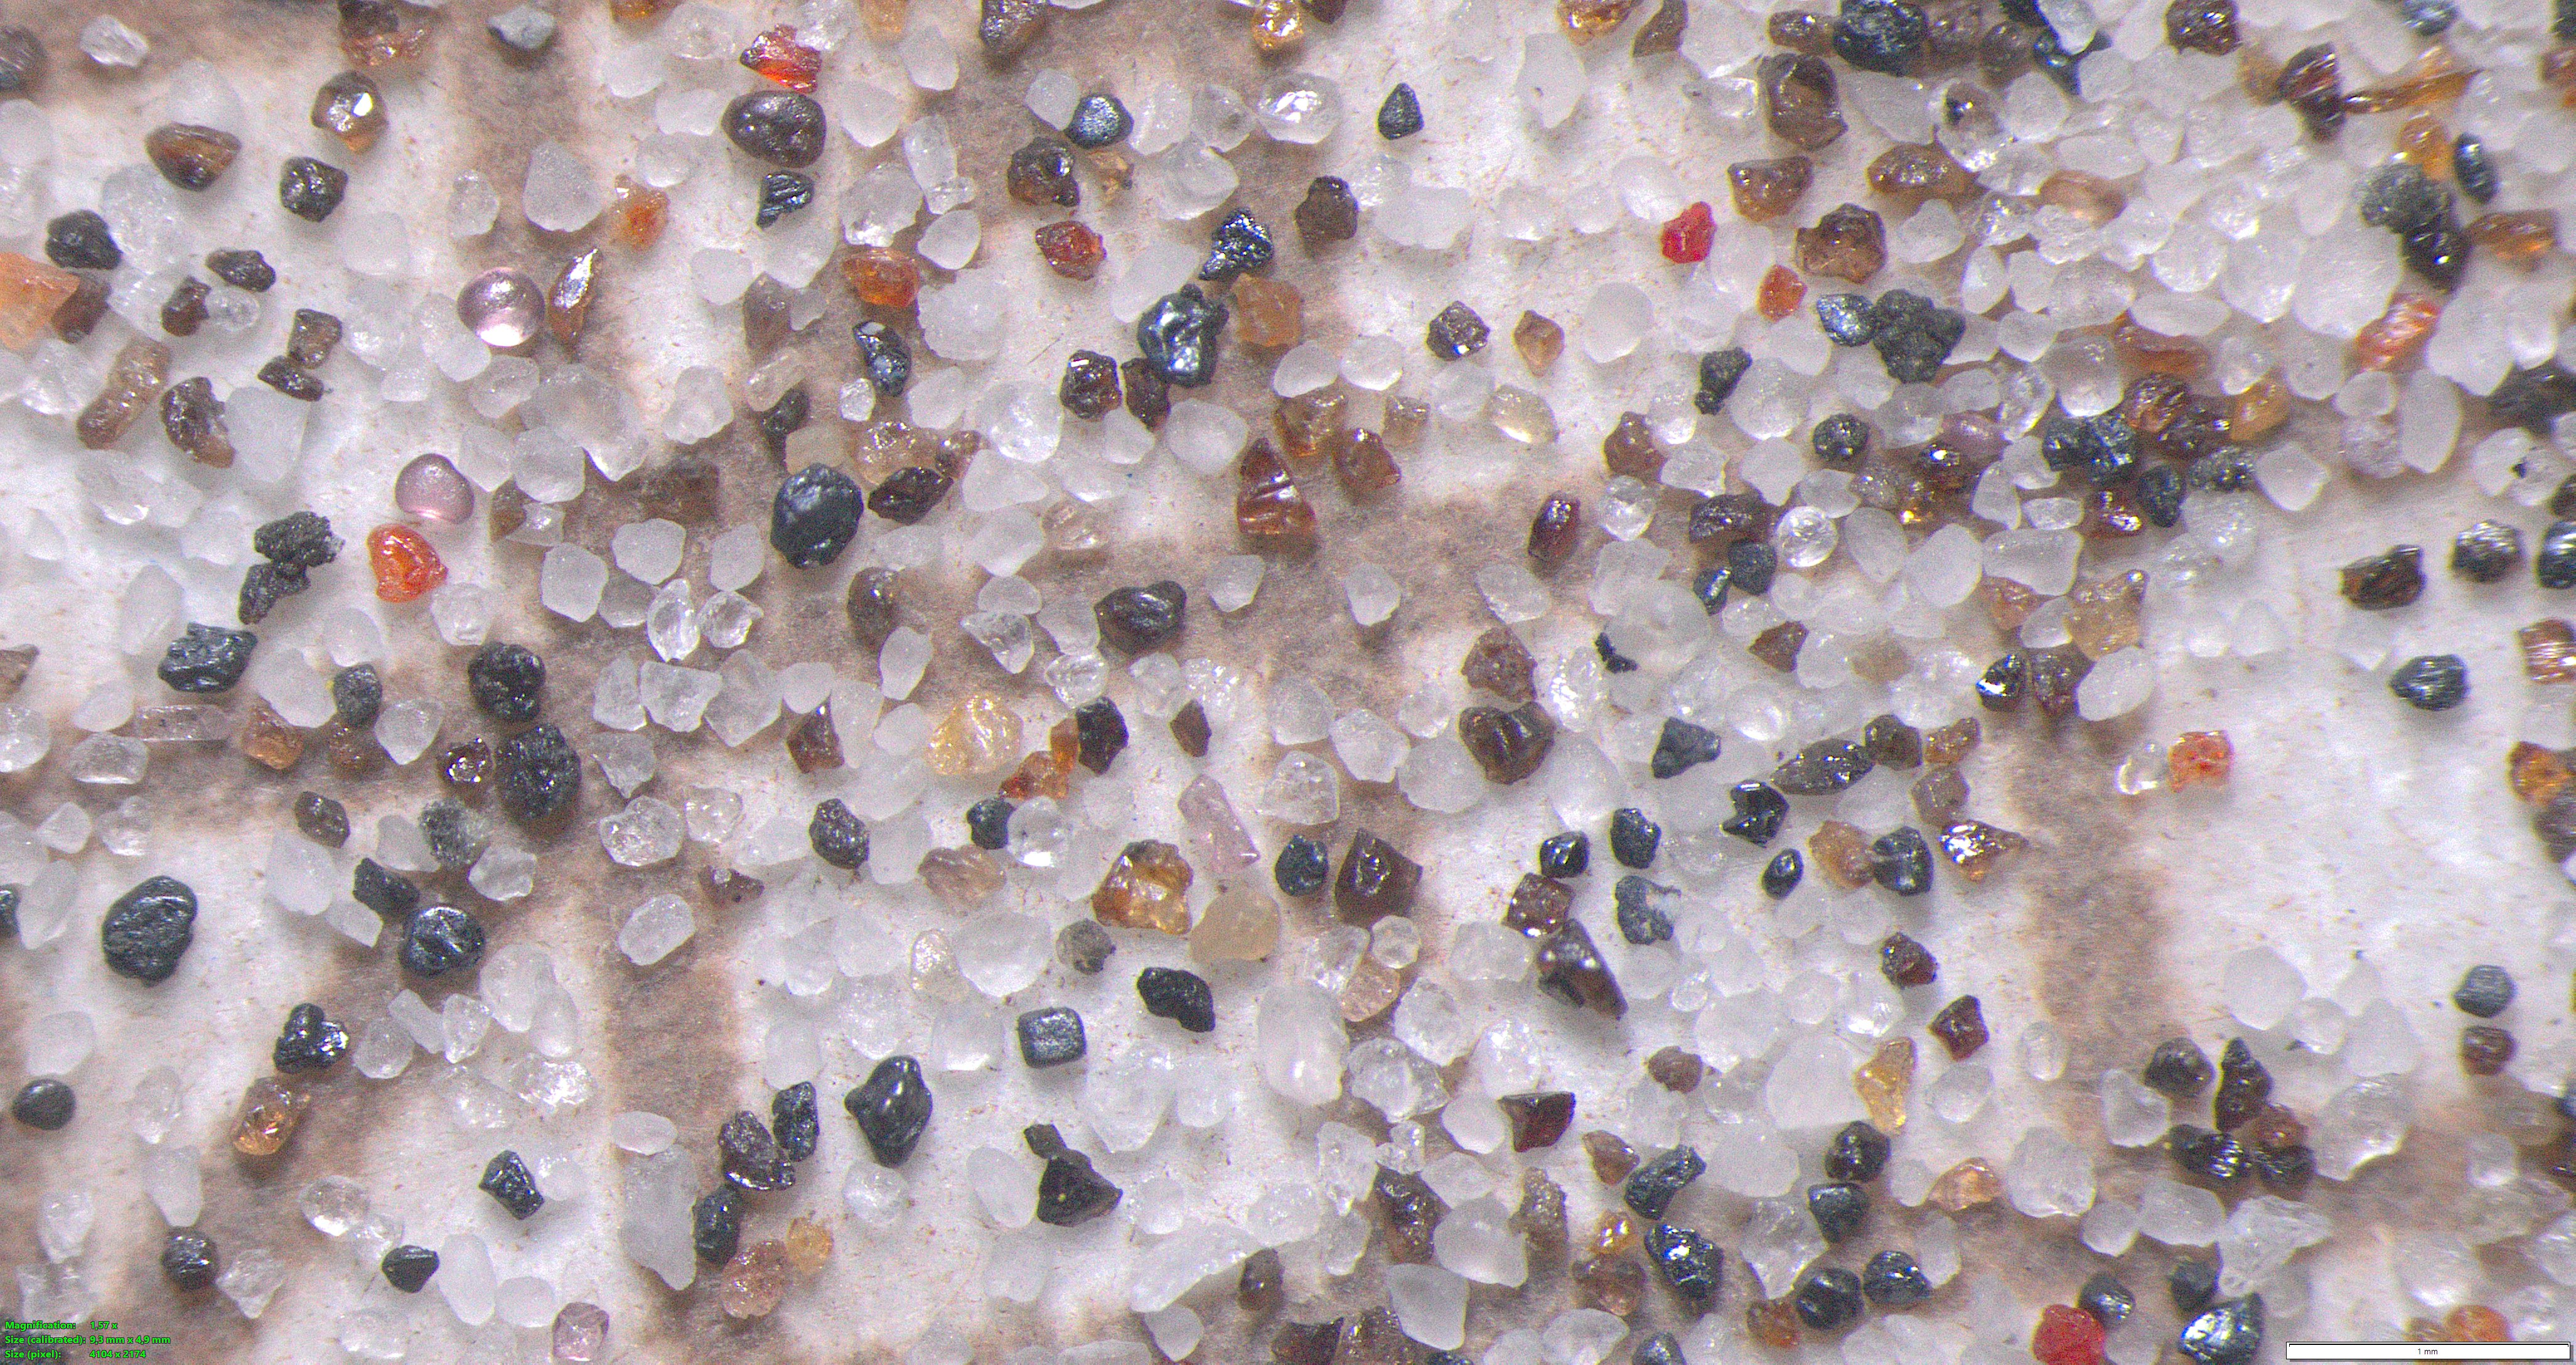
\includegraphics[width=\textwidth]{figure/sebeleumResize.jpg}
%         \caption{Citra Awal tanpa \textit{Flip}}
%         \label{fig:4.CitraAwalFlip}
%     \end{subfigure}
    
%     % Baris kedua: satu gambar di bawah tengah
%     \vskip\baselineskip
%     \begin{subfigure}[b]{0.475\textwidth}
%         \centering
%         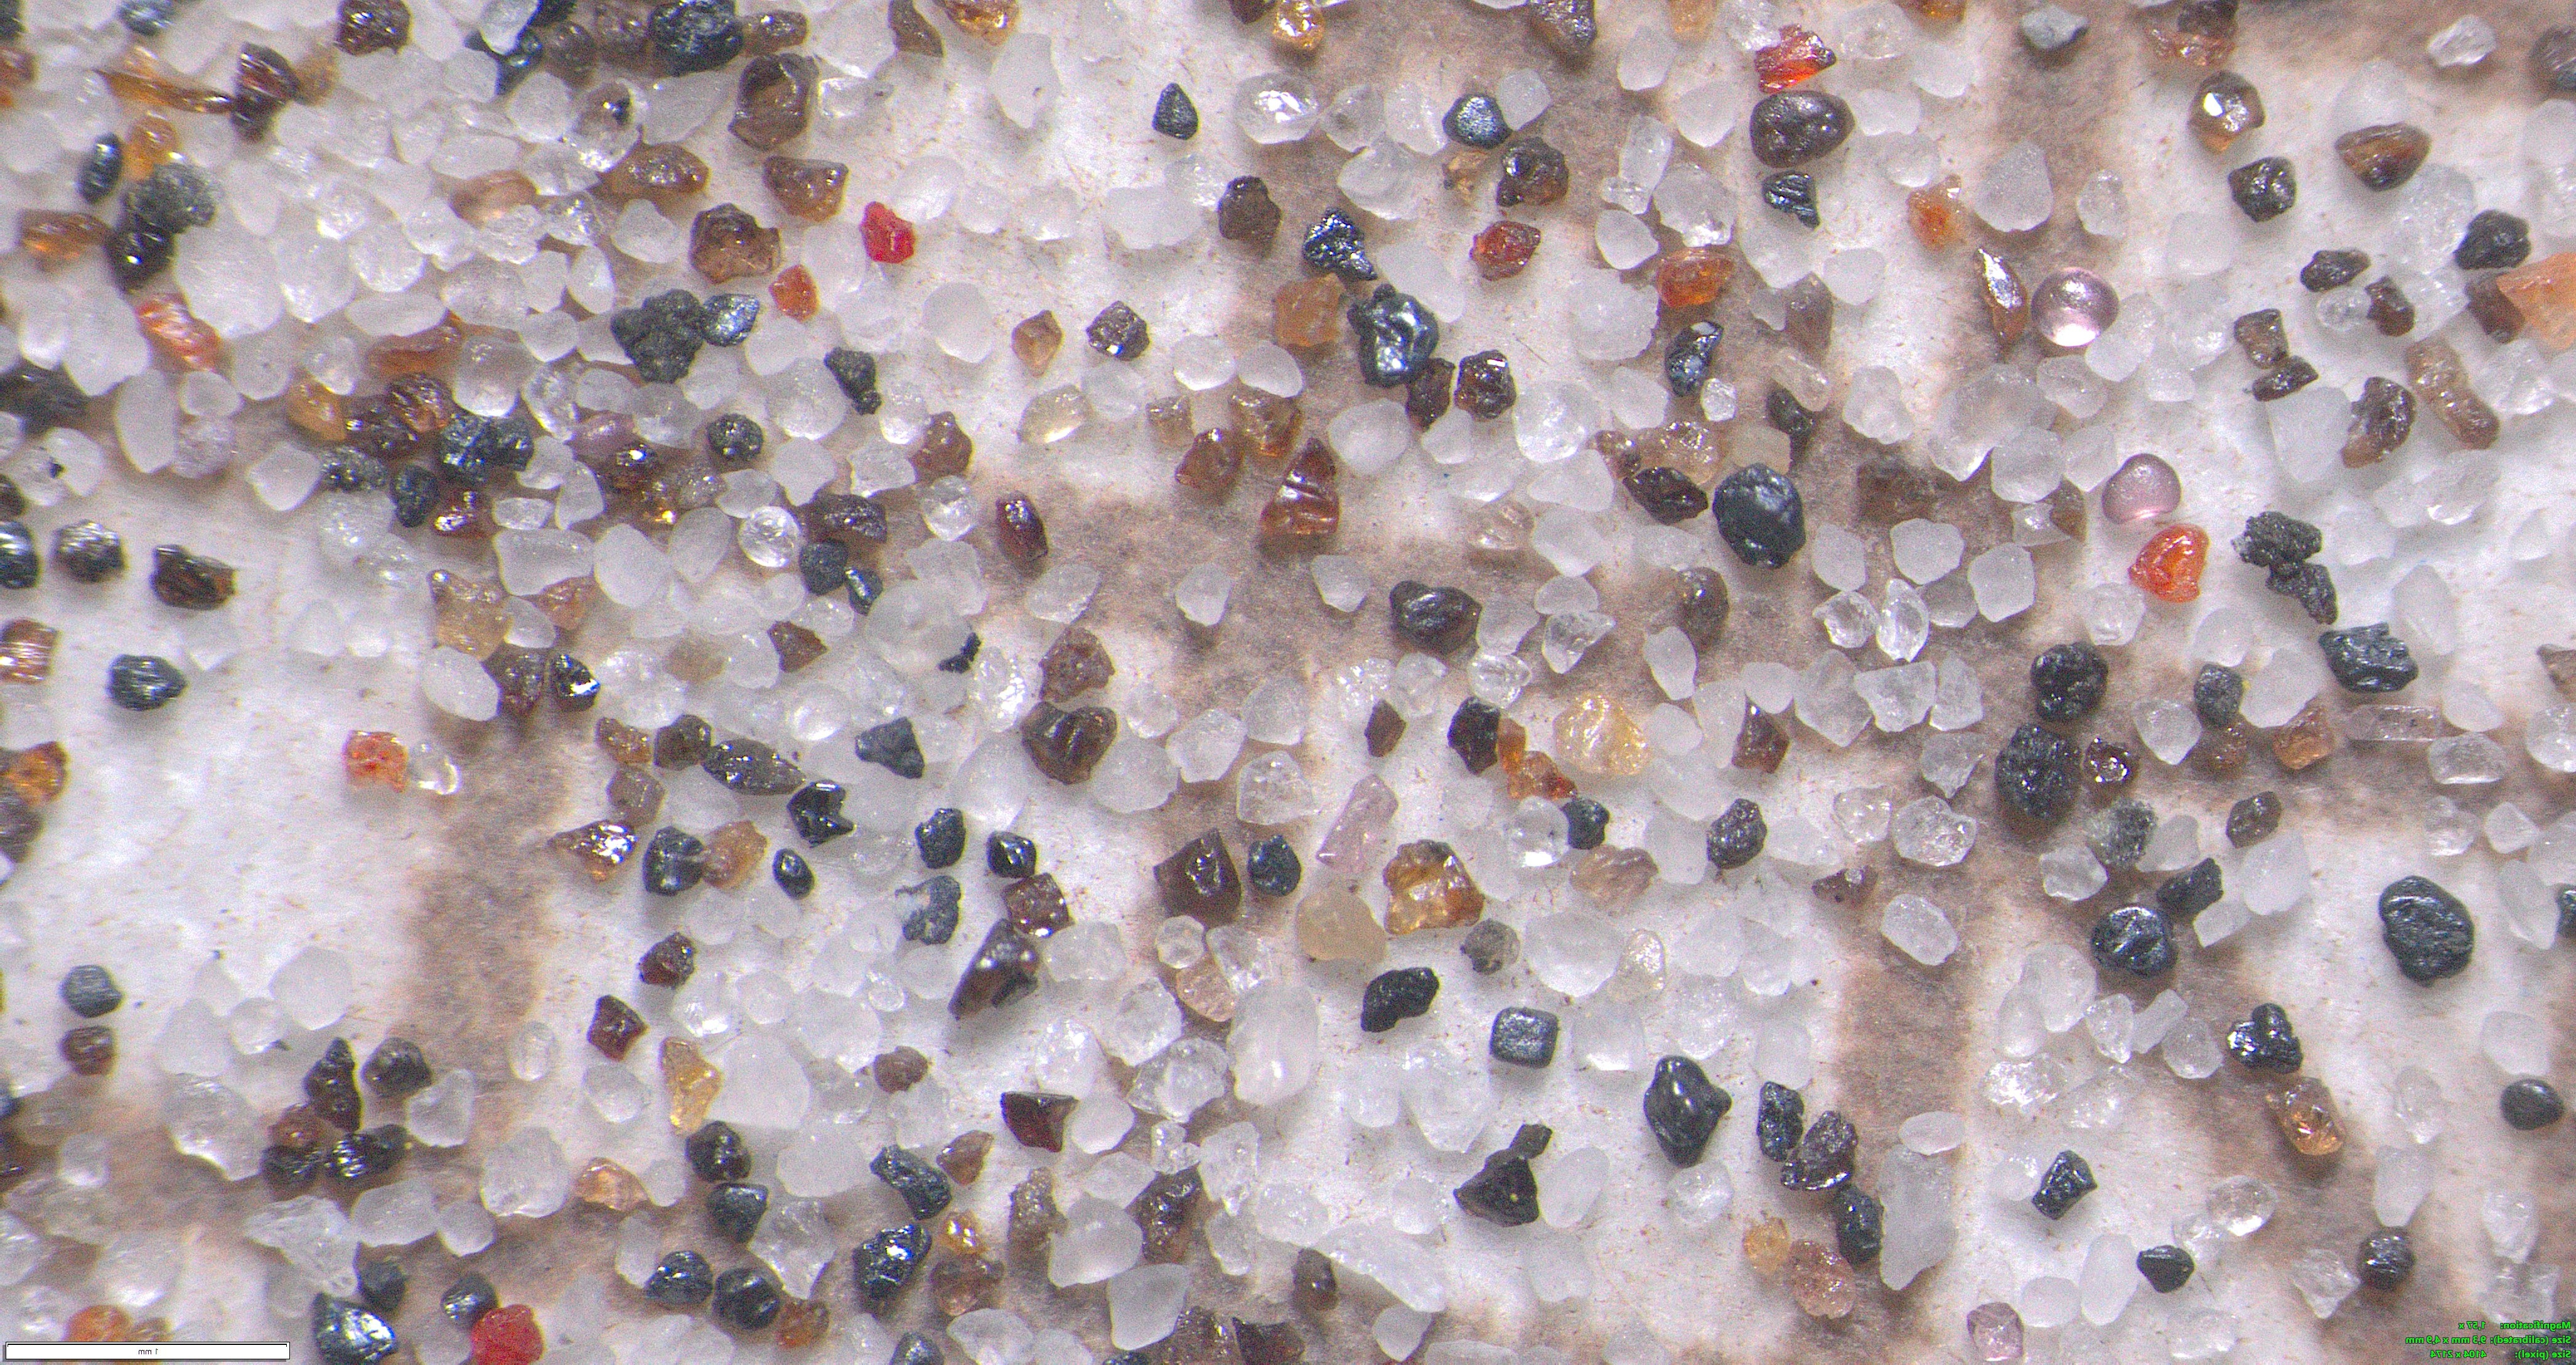
\includegraphics[width=\textwidth]{figure/hasilFlipHorizontal.jpg}
%         \caption{Hasil \textit{Flip} Horizontal ($\curvearrowright$)}
%         \label{fig:4.hasilFlipHorizontal}
%     \end{subfigure}
%     \hfill
%     \begin{subfigure}[b]{0.475\textwidth}
%         \centering
%         \includegraphics[width=\textwidth]{figure/hasilFlipVertical.jpg}
%         % \caption{Hasil \textit{Flip} Vertical ($\shortdownarrow$)}
%         \caption{Hasil \textit{Flip} Vertical (\protect$\downarrow$)}
%         % \caption{Hasil \textit{Flip} Vertical ($\downarrow$)}

%         \label{fig:4.hasilFlipVertical}
%     \end{subfigure}
%     \caption{Hasil \textit{Flip} Data}
%     \label{fig:4.HasilFlipData}
% \end{figure}

\subsubsection*{\textnormal{2. \textit{Rotate}}}
Penerapan augmentasi \textit{rotate} dilakukan menggunakan pustaka \textit{Albumentations} dengan menerapkan fungsi \texttt{A.Rotate(limit=(-15, 15), p=0.5, border\_mode=cv2.BORDER\_CONSTANT)}. Teknik ini menghasilkan variasi sudut orientasi citra kasiterit yang memperkaya data pelatihan tanpa mengubah karakteristik objek. Variasi ini menggunakan range antara -15 dan 15 derajat \texttt{(limit=(-15, 15))} dan probabilitas 0{,}5 \texttt{(p=0.5)} untuk menerapkan augmentasi. Contoh hasil \textit{rotate} ditunjukkan pada Gambar \ref{fig:3.HasilRotateData}. \par

% \begin{figure}[H]
%     \centering
%     % Baris pertama: dua gambar sejajar
%     \begin{subfigure}[b]{0.475\textwidth}
%         \centering
%         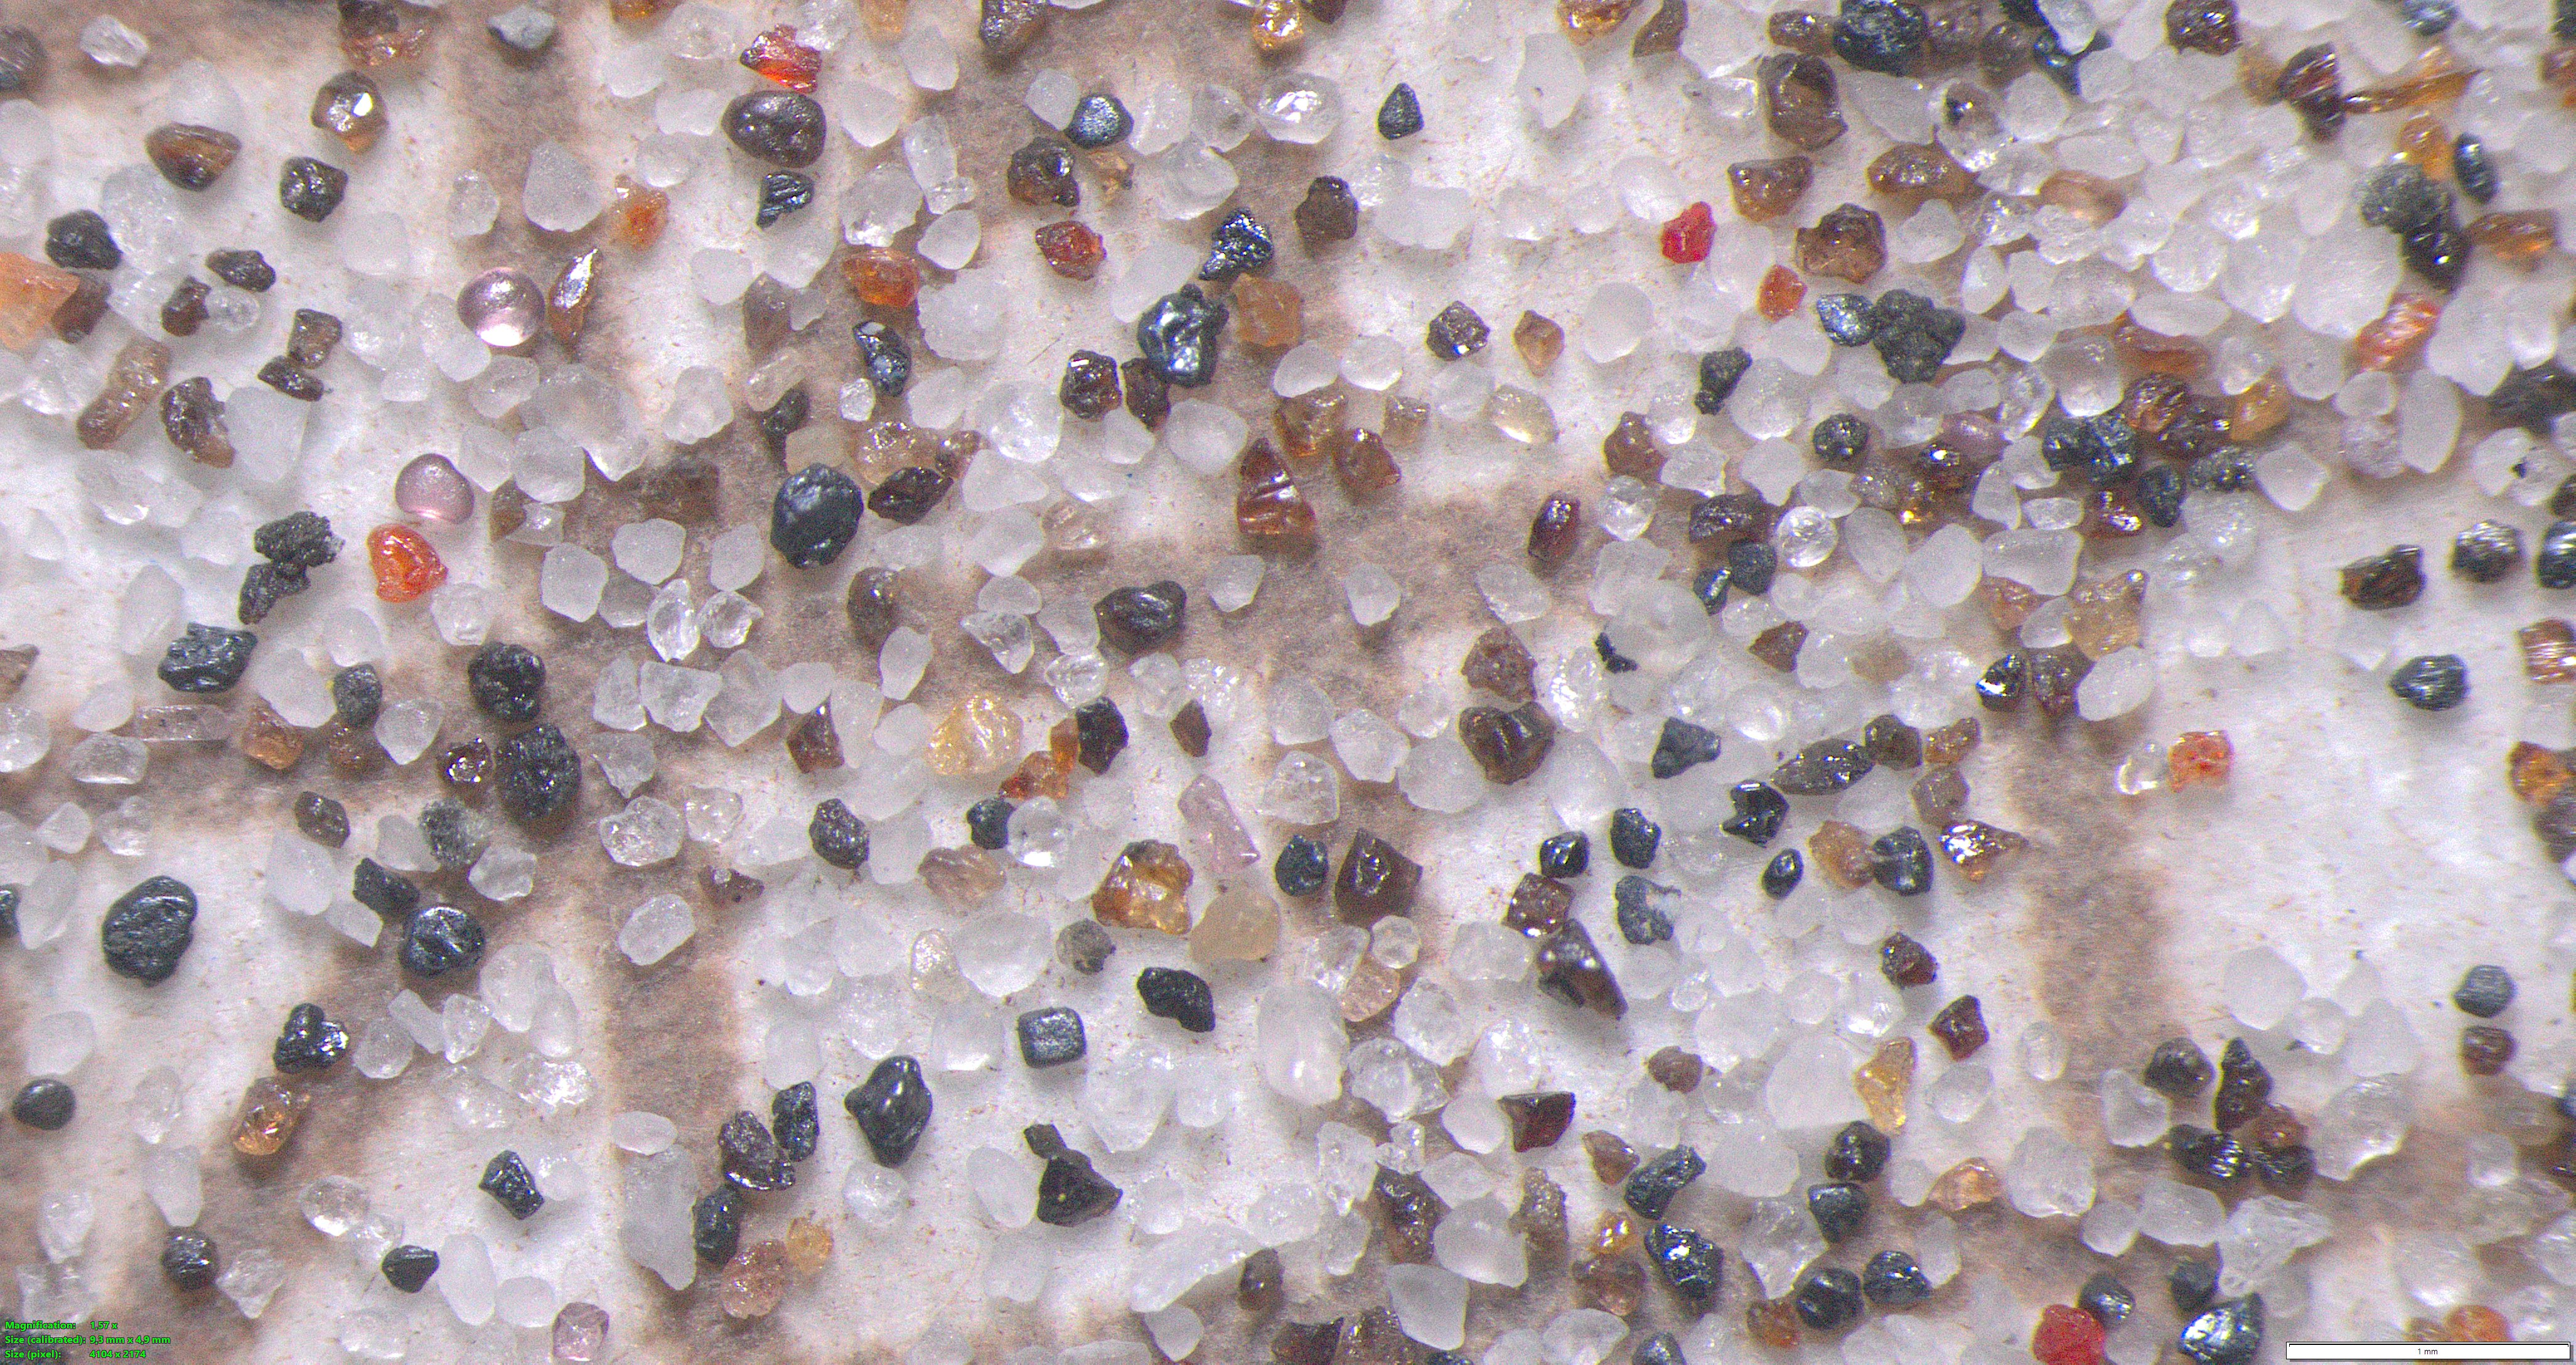
\includegraphics[width=\textwidth]{figure/sebeleumResize.jpg}
%         \caption{Citra Awal tanpa \textit{Rotate}}
%         \label{fig:4.RotateAwal}
%     \end{subfigure}
%     \hfill
%     \begin{subfigure}[b]{0.475\textwidth}
%         \centering
%         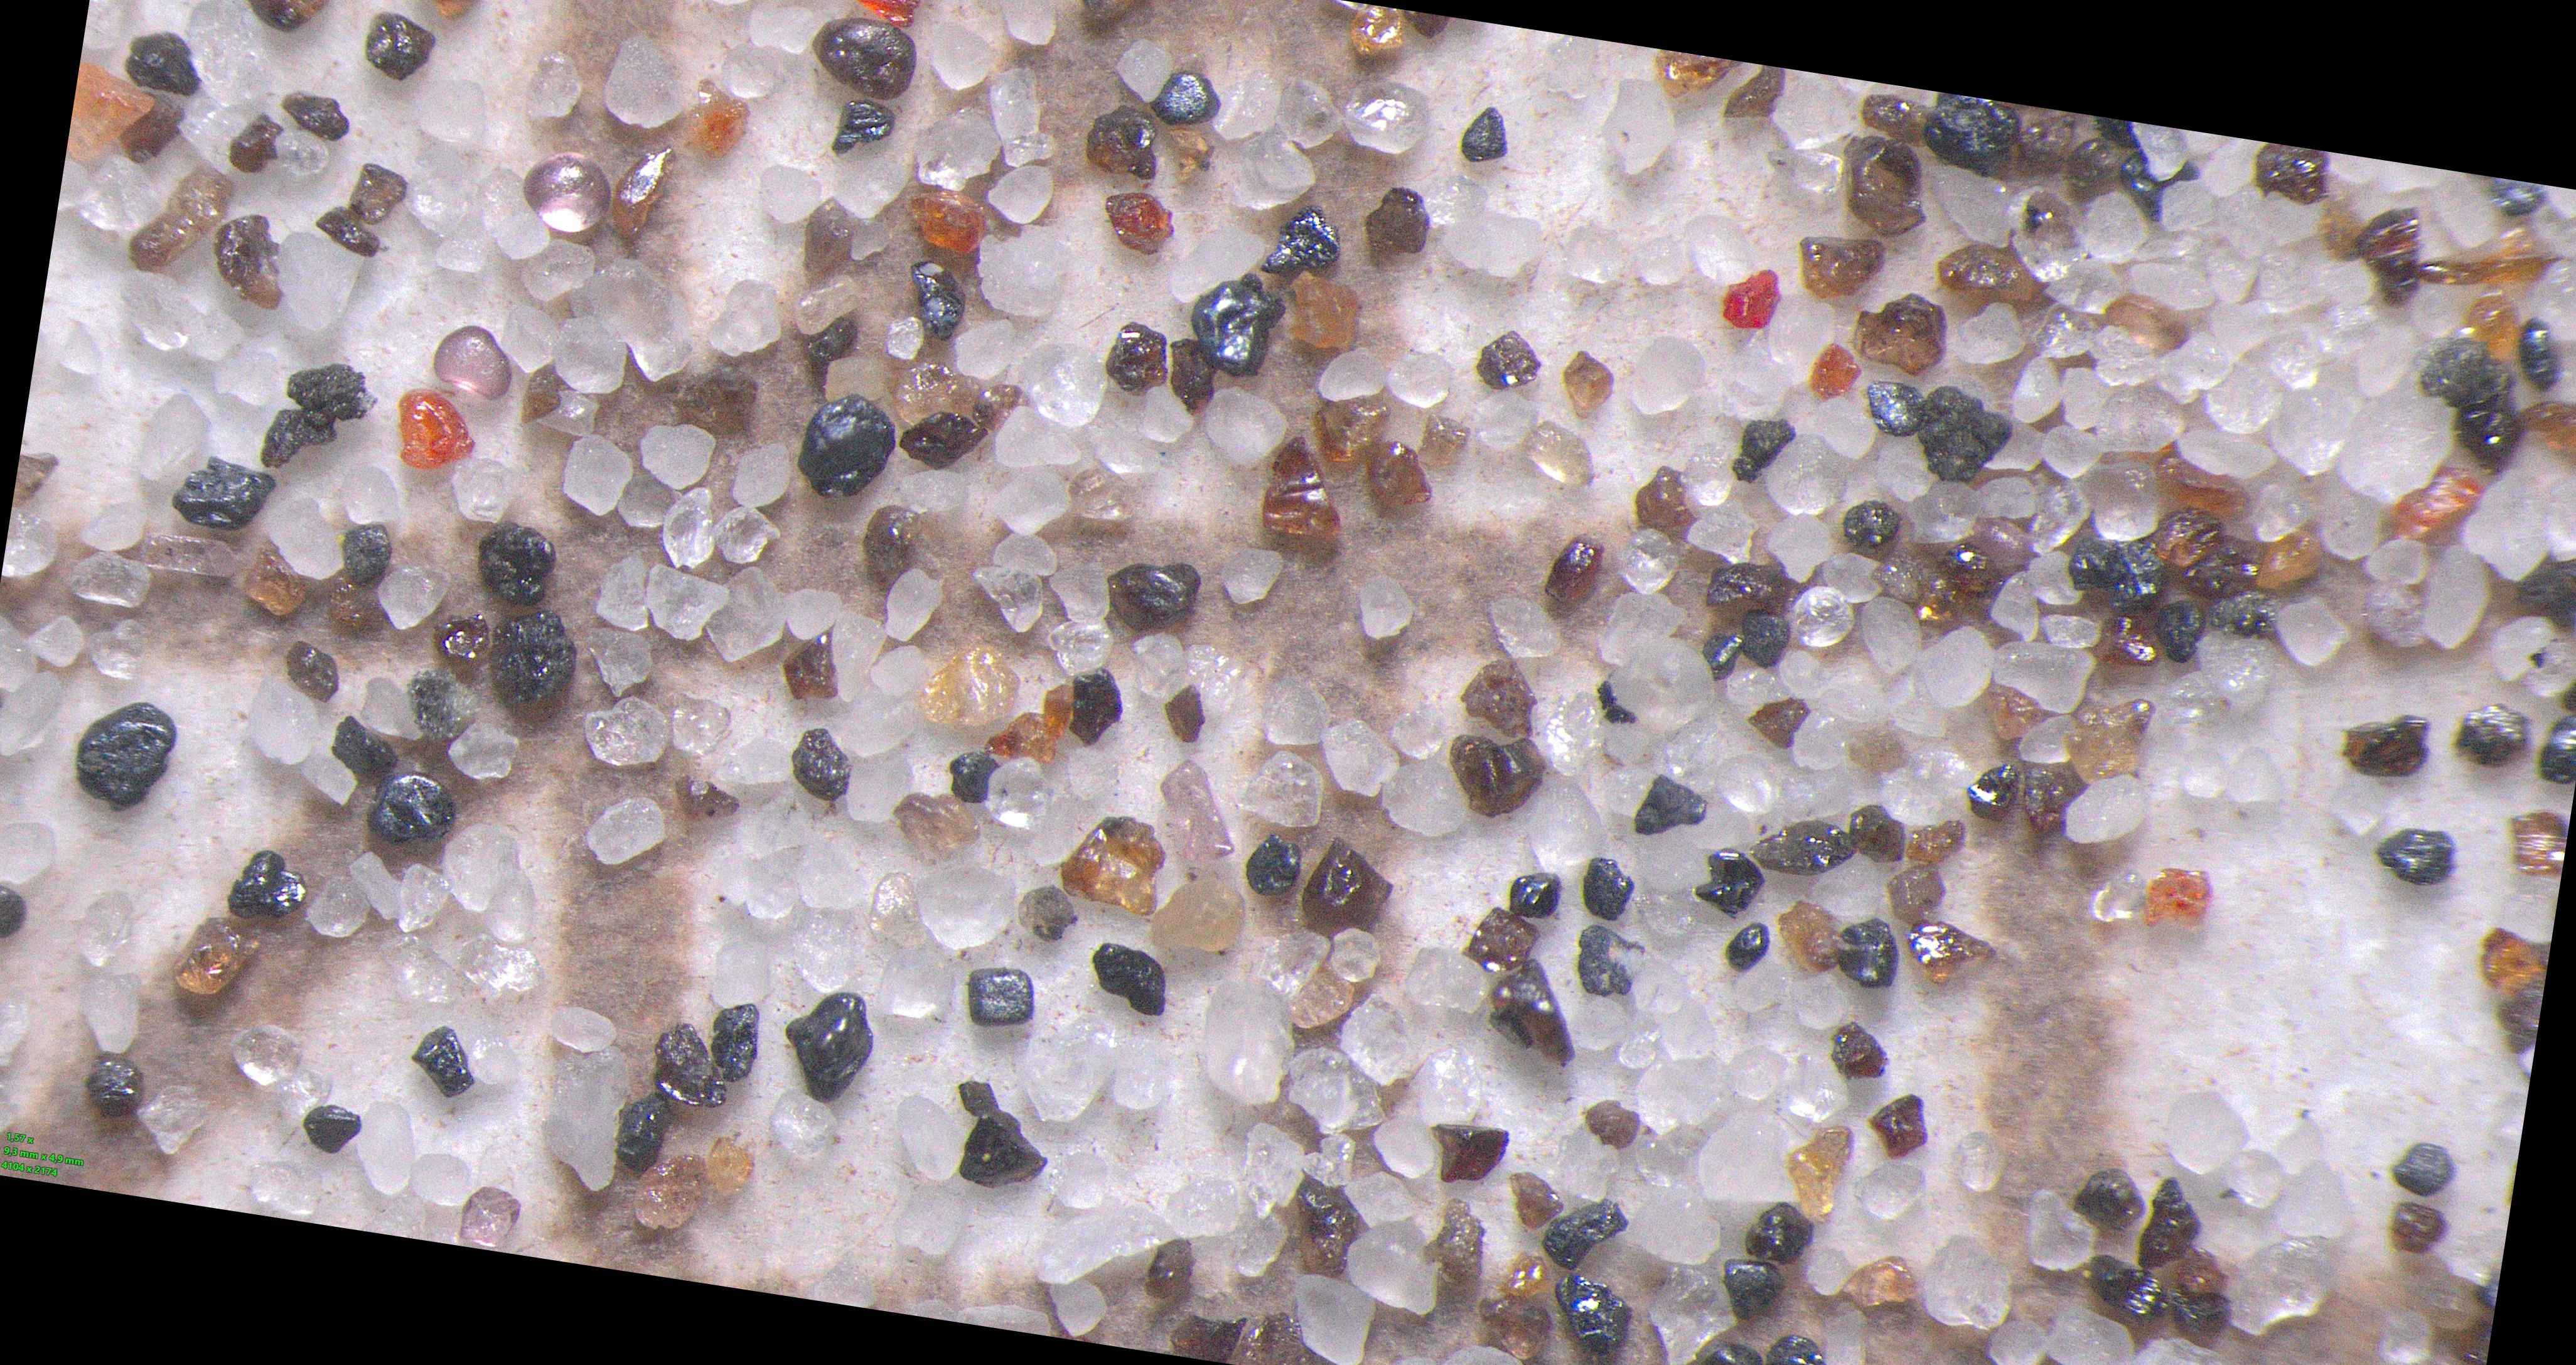
\includegraphics[width=\textwidth]{figure/hasilRotate.jpg}
%         \caption{Hasil \textit{Rotate} dengan 15\textdegree}
%         \label{fig:4.HasilRotate}
%     \end{subfigure}

% 	\caption{Hasil \textit{Rotate} Data}
%     \label{fig:4.HasilRotateData}
% \end{figure}

\subsubsection*{\textnormal{3. \textit{Gaussian Noise}}}
Penerapan augmentasi \textit{Gaussian noise} dilakukan menggunakan pustaka \textit{Albumentations} dengan menerapkan fungsi \texttt{A.GaussNoise(std\_range=(0.44721359549995793928183473374626, 0.44721359549995793928183473374626), mean\_range=(0.0, 0.0), per\_channel=True, p=0.4)}. Teknik ini menghasilkan variasi citra kasiterit dengan gangguan visual ringan tanpa mengubah struktur objek utama. Variasi ini menggunakan standar deviasi 0{,}44721359549995793928183473374626 \texttt{(std\_range=(0.44721359549995793928183473374626, 0.44721359549995793928183473374626))} yang hasilnya variansi 0{,}2 dengan perhitungan yang sudah di jelaskan pada \ref{eq:2.gaussian_distribution} dan menggunakan probabilitas 0{,}4 \texttt{(p=0.4)} untuk menerapkan augmentasi. Contoh hasil \textit{Gaussian noise} ditunjukkan pada Gambar \ref{fig:3.HasilGaussianNoiseData}. \par

% \begin{figure}[H]
%     \centering
%     % Baris pertama: dua gambar sejajar
%     \begin{subfigure}[b]{0.475\textwidth}
%         \centering
%         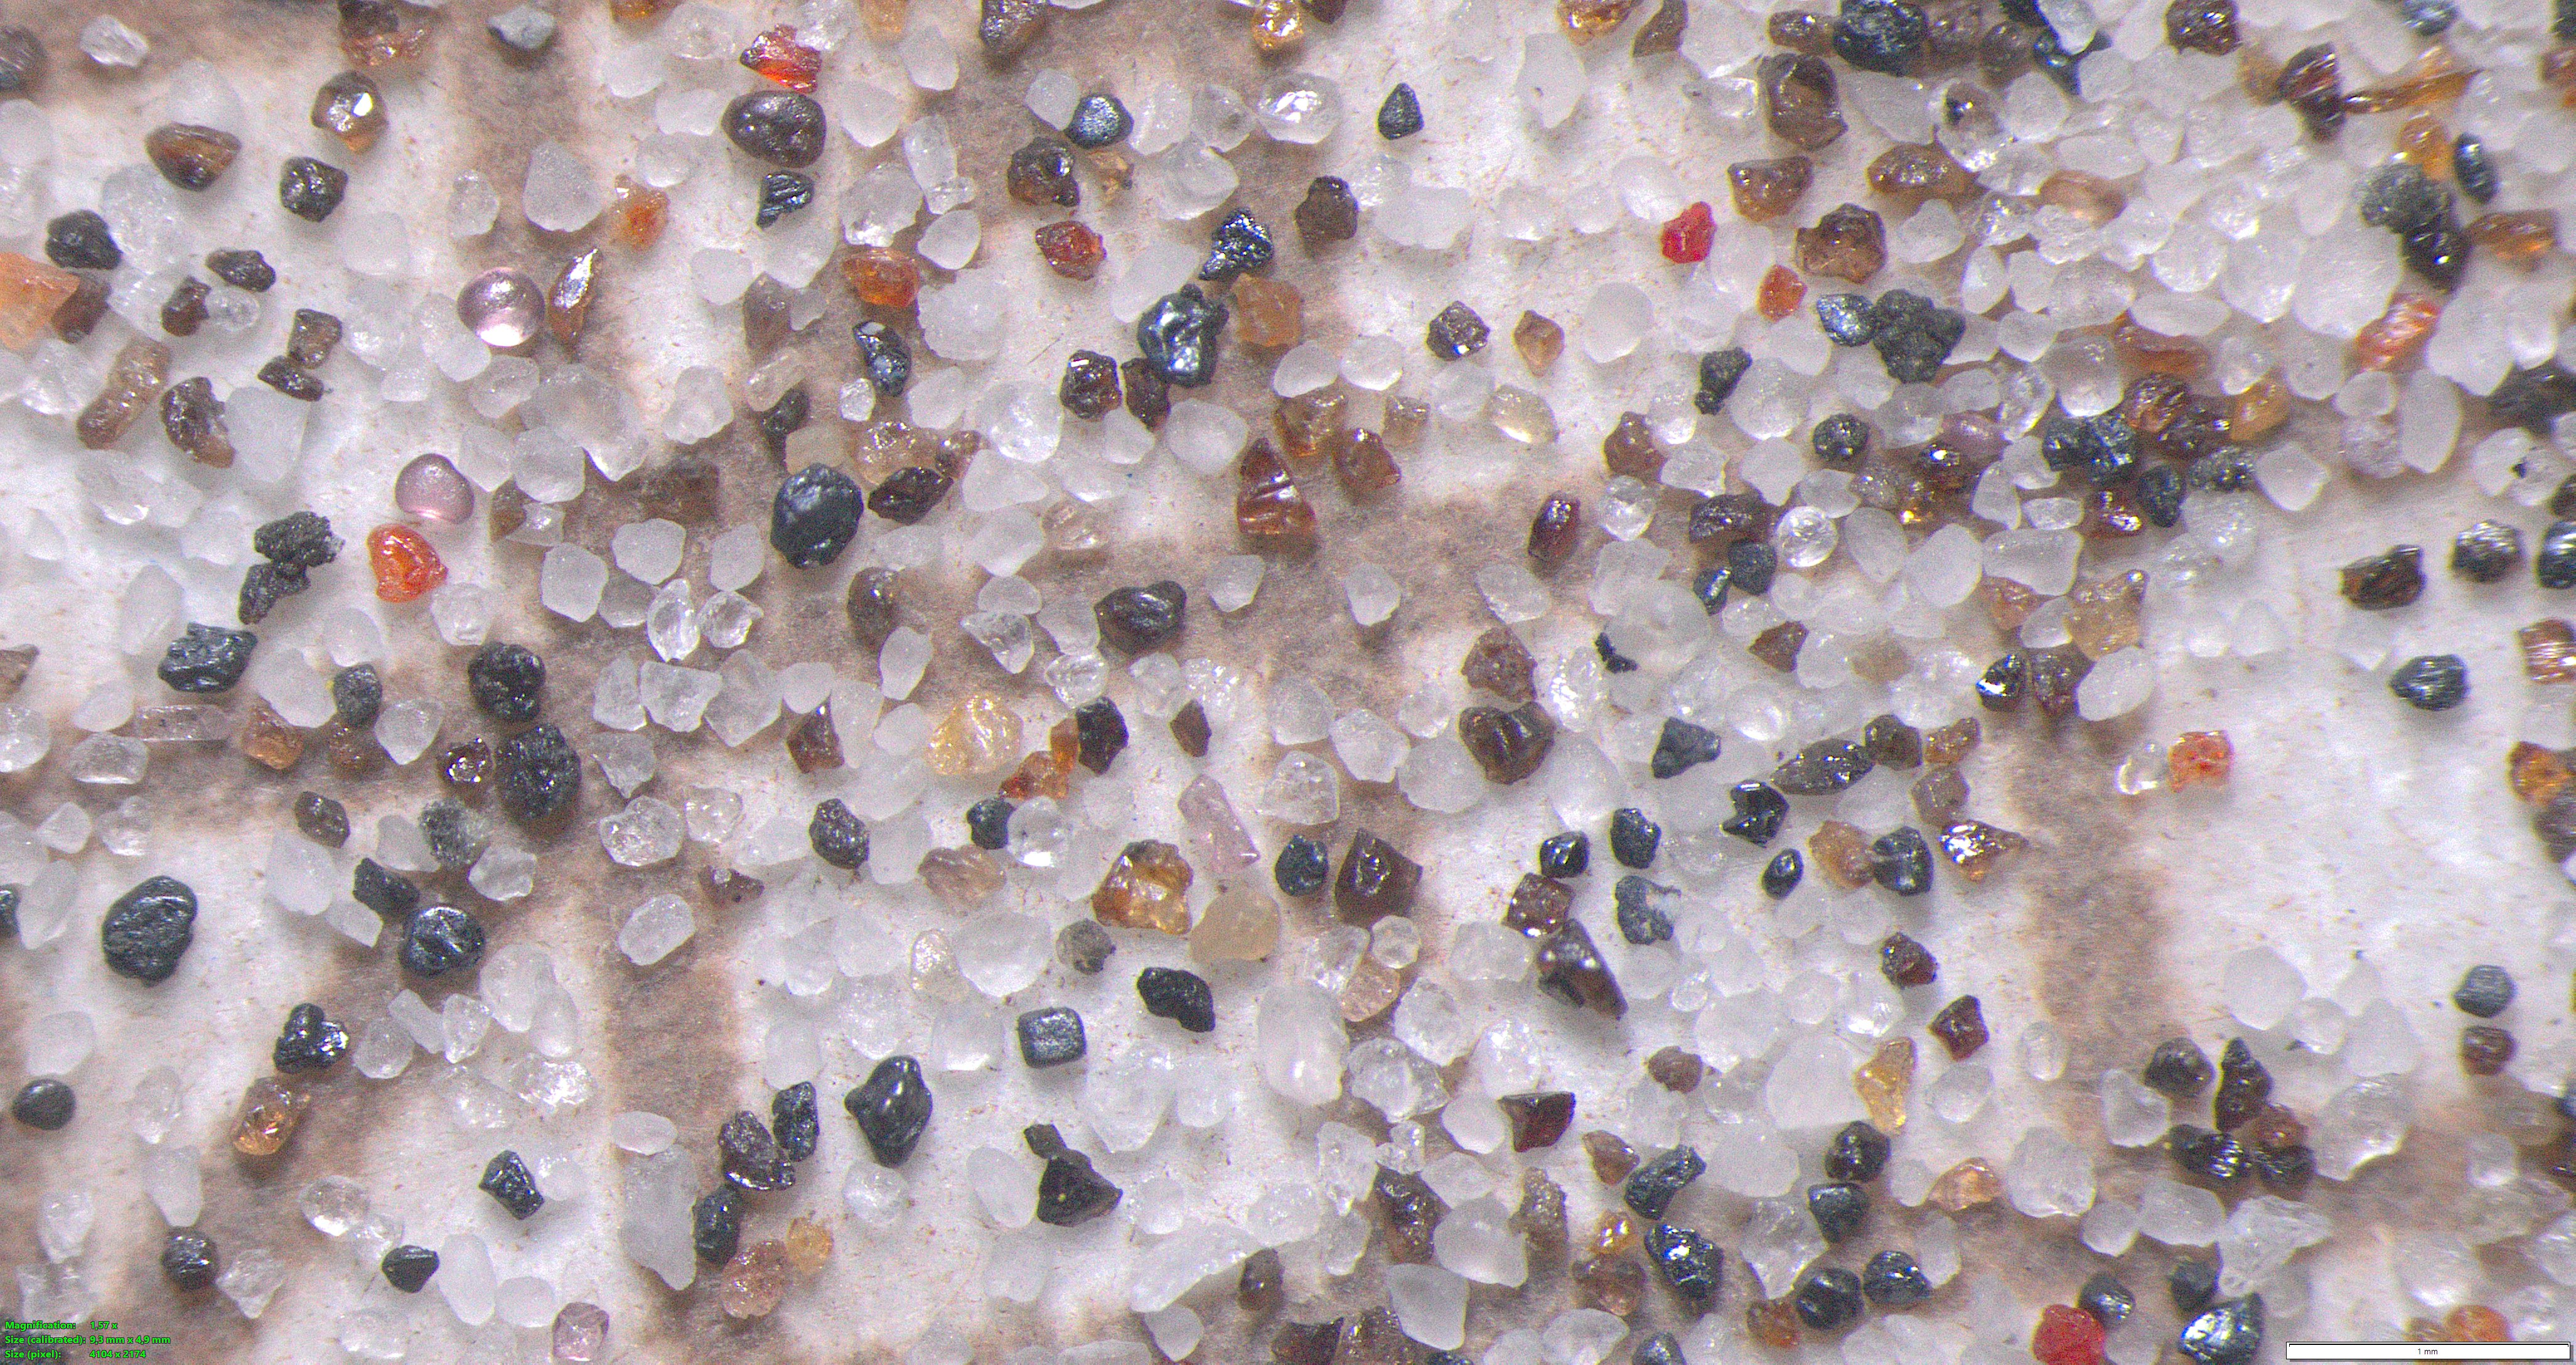
\includegraphics[width=\textwidth]{figure/sebeleumResize.jpg}
%         \caption{Citra Awal tanpa \textit{Gaussian Noise}}
%         \label{fig:4.GaussianAwal}
%     \end{subfigure}
%     \hfill
%     \begin{subfigure}[b]{0.475\textwidth}
%         \centering
%         \includegraphics[width=\textwidth]{figure/hasilGaussianNoise.jpg}
%         \caption{Hasil \textit{Gaussian Noise} dengan variansi 0{,}2}
%         \label{fig:4.HasilGaussianNoise}
%     \end{subfigure}

% 	\caption{Hasil \textit{Gaussian Noise} Data}
%     \label{fig:4.HasilGaussianNoiseData}
% \end{figure}

\subsubsection{\textit{Normalization}}
Penerapan \textit{normalization} atau normalisasi menghasilkan citra dengan rentang nilai piksel yang seragam, sehingga data pelatihan menjadi lebih stabil dan konsisten. Proses ini dilakukan dengan menggunakan nilai \textit{mean} [0{,}0, 0{,}0, 0{,}0] dan standar deviasi [1{,}0, 1{,}0, 1{,}0], sehingga nilai piksel dinormalisasi dengan rata-rata nol dan variansi satu. Kondisi ini mendukung stabilitas proses pelatihan dan meningkatkan efektivitas pembelajaran model. Kode untuk tahap augmentasi dan normalisasi dapat dilihat pada Kode \ref{code:4.code_augmentasi_normalisasi}. \par

% Menulis blok kode
\begin{lstlisting}[caption={Proses Augmentasi dan Normalisasi}, label={code:4.code_augmentasi_normalisasi}]
def get_train_transform():
    """
    Augmentasi tipis untuk training - flip, rotate, noise ringan.
    """
    return A.Compose([
        A.HorizontalFlip(p=0.4),
        A.VerticalFlip(p=0.4),
        A.Rotate(limit=(-15, 15), p=0.5, border_mode=cv2.BORDER_CONSTANT),
        A.GaussNoise(std_range=(0.44721359549995793928183473374626, 0.44721359549995793928183473374626), mean_range=(0.0, 0.0), per_channel=True, p=0.3), # Gaussian noise dengan variansi 0.2
        A.Normalize(mean=(0.0, 0.0, 0.0), std=(1.0, 1.0, 1.0), max_pixel_value=255.0),
        ToTensorV2(),
    ])


def get_val_transform():
    """
    Transformasi untuk validation - hanya normalisasi.
    """
    return A.Compose([
        A.Normalize(mean=(0.0, 0.0, 0.0), std=(1.0, 1.0, 1.0), max_pixel_value=255.0),
        ToTensorV2(),
    ])

\end{lstlisting}

Tahap augmentasi dan normalisasi citra dapat dilihat pada fungsi \texttt{get\_train\_transform()} yang digunakan untuk menerapkan augmentasi dan juga fungsi \texttt{A.Normalize()} digunakan untuk menormalisasi nilai piksel citra berdasarkan parameter \textit{mean} dan standar deviasi, sementara \texttt{ToTensorV2()} berfungsi untuk mengubah format citra menjadi \textit{tensor} agar dapat diproses oleh model PyTorch. Fungsi \texttt{get\_val\_transform()} juga menerapkan normalisasi dan konversi \textit{tensor} yang sama untuk keperluan validasi agar format data tetap konsisten. \par

\subsection{Pengembangan Model} \label{IV.Pengembangan_Model}
Pada tahap pengembangan model, dilakukan pembagian data menggunakan metode \textit{k-fold cross validation}. Selanjutnya, proses pelatihan dan evaluasi dilaksanakan pada masing-masing arsitektur model yang digunakan dalam penelitian.

\subsubsection{Pembagian Data}
Proses pembagian data dilakukan untuk memisahkan dataset menjadi data pelatihan dan data validasi. Jumlah data yang digunakan berjumlah 537 \textit{tiles}, yang terbagi ke dalam 5 \textit{fold} dengan rasio pembagian 80:20 pada setiap iterasi. Kode yang digunakan untuk proses pembagian data tersebut dapat dilihat pada Kode \ref{code:4.kfold_pembagian_data}. \par
% Menulis blok kode
\begin{lstlisting}[caption={Proses Pembagian Data}, label={code:4.kfold_pembagian_data}]
class CassiteriteDataset(Dataset):
...
    def __getitem__(self, idx):
        # Get image file and tile index
        img_name, tile_id = self.tile_index[idx]
        img_path = os.path.join(self.root_dir, img_name)
        
        # Load full image
        image = cv2.imread(img_path)
        
        if image is None:
            raise ValueError(f"Failed to load image: {img_path}")
        
        image = cv2.cvtColor(image, cv2.COLOR_BGR2RGB)
        original_h, original_w = image.shape[:2]
        
        # Load annotation
        json_name = os.path.splitext(img_name)[0] + '.json'
        json_path = os.path.join(self.root_dir, json_name)

    ...
def prepare_kfold_datasets(root_dir=ROOT_DIR, n_splits=5, grid=(2, 2)):
    """
    Mempersiapkan 5-fold cross-validation datasets dengan automatic splitting.
    """
    # Get all image files
    all_files = [f for f in os.listdir(root_dir) if f.endswith(('.jpg', '.jpeg', '.png'))]
    all_files = sorted(all_files)
    
    print(f"Total images found: {len(all_files)}")
    print(f"Grid split: {grid[0]}x{grid[1]} = {grid[0] * grid[1]} tiles per image")
    
    # Pre-compute semua valid tiles dari semua images
    print("\nPre-computing all valid tiles...")
    all_tiles = []
    for img_file in all_files:
        valid_tiles = get_valid_tiles_from_image(root_dir, img_file, grid)
        all_tiles.extend(valid_tiles)
    
    print(f"Total valid tiles: {len(all_tiles)}")
    
    # K-Fold split pada tiles
    kfold = KFold(n_splits=n_splits, shuffle=True, random_state=42)
    fold_datasets = []
    
    for fold, (train_idx, val_idx) in enumerate(kfold.split(all_tiles)):
        print(f"\nFold {fold + 1}/{n_splits}")
        
        train_tiles = [all_tiles[i] for i in train_idx]
        val_tiles = [all_tiles[i] for i in val_idx]
        
        print(f"  Train tiles: {len(train_tiles)}")
        print(f"  Val tiles: {len(val_tiles)}")
        
        # Create datasets dengan tile_list langsung
        train_dataset = CassiteriteDataset(
            root_dir=root_dir,
            tile_list=train_tiles,
            grid=grid,
            transform=get_train_transform(),
            is_train=True
        )
        
        val_dataset = CassiteriteDataset(
            root_dir=root_dir,
            tile_list=val_tiles,
            grid=grid,
            transform=get_val_transform(),
            is_train=False
        )
        
        fold_datasets.append((train_dataset, val_dataset))
    
    return fold_datasets
\end{lstlisting}

Kelas \textit{CassiteriteDataset} berfungsi untuk memuat citra dan anotasi berdasarkan indeks \textit{tile}. Metode \texttt{\_\_getitem\_\_()} melakukan pembacaan citra dalam format RGB dan pemuatan anotasi JSON yang disesuaikan secara otomatis dengan nama berkas citra, sebagaimana ditunjukkan pada baris 18 dan 19 Kode~\ref{code:4.kfold_pembagian_data}. Sementara itu, fungsi \texttt{prepare\_kfold\_datasets()} bertugas mengumpulkan seluruh \textit{tile} valid melalui \texttt{get\_valid\_tiles\_from\_image()} dan membaginya ke dalam lima \textit{fold} menggunakan metode \textit{K-Fold Cross Validation}. Dalam setiap iterasi, indeks \textit{tile} dipisahkan menjadi \textit{train\_tiles} dan \textit{val\_tiles} untuk inisialisasi objek \textit{CassiteriteDataset} dengan transformasi yang sesuai. Seluruh pasangan dataset pelatihan dan validasi kemudian disimpan dalam variabel \textit{fold\_datasets} untuk tahap pelatihan, dengan ringkasan pembagian data yang disajikan pada Tabel~\ref{table:4.pembagian_kfold}. \par

\begin{table}[H]
\centering
\caption{Ilustrasi \textit{K-Fold Cross Validation}}
\label{table:4.pembagian_kfold}
\begin{tabular}{|c|c|c|c|c|c|c|c|}
\hline
\multirow{2}{*}{\textbf{Iterasi}} & \multicolumn{5}{c|}{\textbf{\textit{K-Fold}}} & \multicolumn{2}{c|}{\textbf{Data}} \\
\cline{2-8}
& \textbf{1} & \textbf{2} & \textbf{3} & \textbf{4} & \textbf{5} & \textbf{\textit{Train}} & \textbf{\textit{Validation}} \\
\hline
1 & \cellcolor{blue!20}108 & 108 & 107 & 107 & 107 & 429 & 108 \\
\hline
2 & 108 & \cellcolor{blue!20}108 & 107 & 107 & 107 & 429 & 108 \\
\hline
3 & 108 & 108 & \cellcolor{blue!20}107 & 107 & 107 & 430 & 107 \\
\hline
4 & 108 & 108 & 107 & \cellcolor{blue!20}107 & 107 & 430 & 107 \\
\hline
5 & 108 & 108 & 107 & 107 & \cellcolor{blue!20}107 & 430 & 107 \\
\hline
\multicolumn{6}{|c|}{\textbf{Total Keseluruhan \textit{Tiles}}} & \multicolumn{2}{c|}{\textbf{537}} \\
\hline
\end{tabular}

\end{table}
Pada Tabel \ref{table:4.pembagian_kfold} terlihat bahwa dataset dibagi menjadi data pelatihan (\textit{train}) dan data validasi (\textit{validation}). Pada proses \textit{k-fold cross validation} dengan lima \textit{fold}, setiap blok berwarna biru menunjukkan \textit{fold} yang berfungsi sebagai data validasi pada iterasi ke-$n$. Sebagai contoh, pada iterasi pertama Fold 1 yang berisi 108 \textit{tiles} digunakan sebagai data validasi, sedangkan Fold 2 hingga Fold 5 berperan sebagai data pelatihan dengan total 429 \textit{tiles}. Proses ini berlanjut hingga setiap \textit{fold} mendapatkan giliran menjadi data validasi satu kali. Pada setiap iterasi, jumlah data pelatihan berkisar antara 429--430 \textit{tiles} dan data validasi sebanyak 107--108 \textit{tiles}, bergantung pada distribusi \textit{fold} yang digunakan. Secara keseluruhan, total \textit{tiles} yang digunakan dalam proses \textit{k-fold cross validation} adalah 537 \textit{tiles}. \par

\subsubsection{Pelatihan Model}
Pelatihan model akan dilakukan dengan menggunakan model \textit{pre-trained} \textit{Mask} R-CNN ResNet50 FPN V1 dan \textit{Mask} R-CNN ResNet50 FPN V2 yang sudah ada di \textit{library} PyTorch. \par

\subsubsection*{\textnormal{1. Pendefinisian model \textit{pre-trained} \textit{Mask} R-CNN ResNet50 FPN V1}}
Pada tahap ini dilakukan pendefinisian model \textit{pre-trained} \textit{Mask} R-CNN dengan \textit{backbone} ResNet50 FPN V1 yang digunakan sebagai dasar pelatihan dalam penelitian ini.

% Menulis blok kode
\begin{lstlisting}[caption={Pendefinisian Model \textit{pre-trained} \textit{Mask} R-CNN ResNet50 FPN V1}, label={code:4.definisi_v1}]
def get_maskrcnn_resnet50_fpn_v1(num_classes=2, trainable_layers=3):
    """
    Create Mask R-CNN with ResNet50 + FPN V1 pretrained on COCO.
        model: Mask R-CNN V1 with COCO pretrained weights
    """
    # Load pretrained Mask R-CNN V1 with COCO weights
    model = maskrcnn_resnet50_fpn(
        weights=MaskRCNN_ResNet50_FPN_Weights.COCO_V1,
        trainable_backbone_layers=trainable_layers
    )
    
    # Replace box predictor for custom num_classes
    in_features = model.roi_heads.box_predictor.cls_score.in_features
    model.roi_heads.box_predictor = FastRCNNPredictor(in_features, num_classes)
    
    # Replace mask predictor for custom num_classes
    in_features_mask = model.roi_heads.mask_predictor.conv5_mask.in_channels
    hidden_layer = 256
    model.roi_heads.mask_predictor = MaskRCNNPredictor(
        in_features_mask,
        hidden_layer,
        num_classes
    )
    
    return model
\end{lstlisting}

Fungsi \texttt{get\_maskrcnn\_resnet50\_fpn\_v1()} pada Kode \ref{code:4.definisi_v1} digunakan untuk membangun model \textit{Mask} R-CNN dengan \textit{backbone} ResNet50 FPN V1 yang telah dilatih sebelumnya menggunakan dataset COCO. Parameter \texttt{num\_classes=2} menentukan jumlah kelas keluaran, yaitu satu kelas untuk objek kasiterit dan satu kelas untuk latar belakang, sedangkan \texttt{trainable\_layers=3} mengatur jumlah lapisan \textit{backbone} yang dapat dilatih ulang selama proses \textit{fine-tuning}. Model dimuat dengan bobot \textit{pre-trained} melalui \texttt{MaskRCNN\_ResNet50\_FPN\_Weights.COCO\_V1}. Selanjutnya, komponen \textit{box predictor} diganti menggunakan \texttt{FastRCNNPredictor} untuk menyesuaikan jumlah fitur masukan dengan jumlah kelas yang baru, dan komponen \textit{mask predictor} diganti menggunakan \texttt{MaskRCNNPredictor} dengan jumlah \textit{hidden layer} sebanyak 256 untuk menghasilkan \textit{mask} segmentasi yang sesuai dengan jumlah kelas kustom. \par

\subsubsection*{\textnormal{2. Pendefinisian model \textit{pre-trained} \textit{Mask} R-CNN ResNet50 FPN V2}}
Pada tahap ini dilakukan pendefinisian model \textit{pre-trained} \textit{Mask} R-CNN dengan \textit{backbone} ResNet50 FPN V2 yang digunakan sebagai dasar pelatihan dalam penelitian ini.

% Menulis blok kode
\begin{lstlisting}[caption={Pendefinisian Model \textit{pre-trained} \textit{Mask} R-CNN ResNet50 FPN V2}, label={code:4.definisi_v2}]
def get_maskrcnn_resnet50_fpn_v2(num_classes=2, trainable_layers=3):
    """
    Create Mask R-CNN with ResNet50 + FPN V2 pretrained on COCO.
        model: Mask R-CNN V2 with COCO pretrained weights
    """
    # Load pretrained Mask R-CNN V2 with COCO weights
    model = maskrcnn_resnet50_fpn_v2(
        weights=MaskRCNN_ResNet50_FPN_V2_Weights.COCO_V1,
        trainable_backbone_layers=trainable_layers
    )
    
    # Replace box predictor for custom num_classes
    in_features = model.roi_heads.box_predictor.cls_score.in_features
    model.roi_heads.box_predictor = FastRCNNPredictor(in_features, num_classes)
    
    # Replace mask predictor for custom num_classes
    in_features_mask = model.roi_heads.mask_predictor.conv5_mask.in_channels
    hidden_layer = 256
    model.roi_heads.mask_predictor = MaskRCNNPredictor(
        in_features_mask,
        hidden_layer,
        num_classes
    )
    
    return model
\end{lstlisting}

Fungsi \texttt{get\_maskrcnn\_resnet50\_fpn\_v2()} pada Kode \ref{code:4.definisi_v2} digunakan untuk membangun model \textit{Mask} R-CNN dengan \textit{backbone} ResNet50 FPN V2 yang merupakan versi terbaru dengan arsitektur yang lebih optimal dibandingkan V1. Parameter \texttt{num\_classes=2} menentukan jumlah kelas keluaran untuk objek kasiterit dan latar belakang, sedangkan \texttt{trainable\_layers=3} mengatur jumlah lapisan \textit{backbone} yang dapat dilatih ulang. Model dimuat dengan bobot \textit{pre-trained} melalui \texttt{MaskRCNN\_ResNet50\_FPN\_V2\_Weights.COCO\_V1}. Serupa dengan versi V1, komponen \textit{box predictor} diganti menggunakan \texttt{FastRCNNPredictor} untuk menyesuaikan jumlah fitur masukan dengan jumlah kelas baru, dan komponen \textit{mask predictor} diganti menggunakan \texttt{MaskRCNNPredictor} dengan jumlah \textit{hidden layer} sebanyak 256 untuk menghasilkan \textit{mask} segmentasi sesuai jumlah kelas kustom. 

\subsubsection*{\textnormal{3. Proses Pelatihan Model per Epoch}}
Pada tahap ini dilakukan proses pelatihan model untuk setiap \textit{epoch} menggunakan data pelatihan pada masing-masing \textit{fold}. Proses pelatihan bertujuan untuk memperbarui bobot model secara iteratif berdasarkan nilai \textit{loss} yang dihasilkan dari prediksi dan anotasi \textit{ground truth}. \par

\begin{lstlisting}[caption={Proses Pelatihan Model per Epoch}, label={code:4.train_one_epoch}]
def train_one_epoch(model, dataloader, optimizer, device, epoch,            scheduler=None, scaler=None, use_amp=False,                     warmup_iters=0, warmup_factor=0.1, global_step=0,               base_lr=0.0001, model_type='standard'):

    model.train()
    loss_meter = AverageMeter()
    amodal_loss_meter = AverageMeter()  # Track amodal loss separately
    
    pbar = tqdm(dataloader, desc=f'Epoch {epoch}')
    
    for batch_idx, (images, targets) in enumerate(pbar):
        try:
            # Clear cache before processing batch
            if batch_idx > 0:
                torch.cuda.empty_cache()
            
            # Move to device
            images = [img.to(device) for img in images]
            targets = [{k: v.to(device) for k, v in t.items()} for t in targets]
            
            # Manual warmup (avoid scheduler warning)
            if global_step < warmup_iters:
                alpha = global_step / warmup_iters
                warmup_lr = warmup_factor * (1 - alpha) + alpha
                for param_group in optimizer.param_groups:
                    param_group['lr'] = base_lr * warmup_lr
            
            # Forward pass with optional AMP
            if use_amp and scaler is not None:
                with torch.amp.autocast(device_type='cuda', dtype=torch.float16):
                    loss_dict = model(images, targets)
                    losses = sum(loss for loss in loss_dict.values())
                
                optimizer.zero_grad()
                scaler.scale(losses).backward()
                scaler.unscale_(optimizer)
                torch.nn.utils.clip_grad_norm_(model.parameters(), max_norm=10.0)
                scaler.step(optimizer)
                scaler.update()
            else:
                loss_dict = model(images, targets)
                losses = sum(loss for loss in loss_dict.values())
                optimizer.zero_grad()
                losses.backward()
                torch.nn.utils.clip_grad_norm_(model.parameters(), max_norm=10.0)
                optimizer.step()

            global_step += 1
            
            # Update metrics
            loss_meter.update(losses.item(), len(images))
            
            # Track amodal loss separately for amodal models
            if model_type == 'amodal' and 'loss_amodal_mask' in loss_dict:
                amodal_loss_meter.update(loss_dict['loss_amodal_mask'].item(), len(images))
                pbar.set_postfix({
                    'loss': f'{loss_meter.avg:.4f}',
                    'amodal': f'{amodal_loss_meter.avg:.4f}'
                })
            else:
                pbar.set_postfix({'loss': f'{loss_meter.avg:.4f}'})
            
            # Delete tensors to free memory
            del images, targets, loss_dict, losses
            if batch_idx % 10 == 0:  # More aggressive cache clearing
                torch.cuda.empty_cache()
...
    # Return amodal loss if available
    amodal_loss = amodal_loss_meter.avg if amodal_loss_meter.count > 0 else None
    return loss_meter.avg, global_step, amodal_loss
\end{lstlisting}

Fungsi \texttt{train\_one\_epoch()} pada Kode \ref{code:4.train_one_epoch} menunjukkan proses pelatihan model untuk satu \textit{epoch} dengan menggunakan data pelatihan yang dimuat melalui \texttt{dataloader}. Model diatur pada mode \texttt{model.train()} untuk menghitung nilai \textit{loss} berdasarkan keluaran prediksi dan anotasi, kemudian dilakukan proses \textit{backpropagation} untuk memperbarui bobot model menggunakan \texttt{optimizer} yang telah ditentukan. Untuk menjaga stabilitas pelatihan, diterapkan mekanisme \textit{learning rate warm-up} pada tahap awal iterasi serta \textit{gradient clipping} menggunakan \texttt{clip\_grad\_norm\_} untuk mencegah gradien berlebih. Nilai \textit{loss} rata-rata pada setiap \textit{epoch} dicatat menggunakan \texttt{loss\_meter}, sedangkan pada model \textit{amodal} nilai \texttt{loss\_amodal\_mask} juga dipantau secara terpisah melalui \texttt{amodal\_loss\_meter}. \par

\subsubsection*{\textnormal{4. Pelatihan Model \textit{K-Fold Cross-Validation}}}
Pada tahap ini, pelatihan model dilakukan dengan menerapkan metode \textit{k-fold cross-validation}. Fungsi \texttt{train\_one\_epoch()} dipanggil secara iteratif untuk melatih model pada setiap \textit{epoch} menggunakan data pelatihan dari masing-masing \textit{fold}.

\begin{lstlisting}[caption={Proses Pelatihan Model dengan \textit{K-Fold Cross-Validation}}, label={code:4.train_kfold}]
def train_kfold(config):
...
    # Prepare K-Fold datasets
    print("\nPreparing K-Fold datasets...")
    fold_datasets = prepare_kfold_datasets(
        root_dir=config['data_dir'],
        n_splits=config['n_folds']
    )
    
    all_fold_results = []
    total_training_start = time.time()
    
    # Train each fold
    for fold_idx, (train_dataset, val_dataset) in enumerate(fold_datasets):
        fold_num = fold_idx + 1
...
        fold_start_time = time.time()
        
        # Create model configuration directory name
        lr_str = f"{config['lr']:.0e}" if config['lr'] < 0.01 else f"{config['lr']}"
        model_config_dir = f"{config['backbone']}_{config['model_type']}
         _{config['optimizer']}_lr{lr_str}"
...
        # Create fold directory inside configuration directory
        fold_dir = os.path.join(config_output_dir, f'fold{fold_num}')
        os.makedirs(fold_dir, exist_ok=True)
        
        # DataLoaders
        train_loader = get_dataloader(
            train_dataset,
            batch_size=config['batch_size'],
            shuffle=True,
            num_workers=config['num_workers']
        )
        
        val_loader = get_dataloader(
            val_dataset,
            batch_size=config['batch_size'],
            shuffle=False,
            num_workers=config['num_workers']
        )
        
        # Create model
        print(f"Creating {config['model_type']} model...")
        model = get_model(
            num_classes=config['num_classes'],
            model_type=config['model_type'],
            backbone=config['backbone'],
            trainable_layers=config['trainable_layers']
        )
        model = model.to(device)
        count_parameters(model)
        
        # Optimizer
        params = [p for p in model.parameters() if p.requires_grad]
        if config['optimizer'] == 'sgd':
            optimizer = optim.SGD(
                params, 
                lr=config['lr'], 
                momentum=config.get('momentum', 0.9),
                weight_decay=config['weight_decay']
            )
        elif config['optimizer'] == 'adam':
            optimizer = optim.Adam(
                params, 
                lr=config['lr'], 
                weight_decay=config['weight_decay']
            )
...
        # Main scheduler: CosineAnnealingWarmRestarts
        scheduler = CosineAnnealingWarmRestarts(
            optimizer, 
            T_0=config.get('COSINE_T0', 20),
            T_mult=config.get('COSINE_T_MULT', 1),
            eta_min=config.get('COSINE_ETA_MIN', 1e-6)
        )
        
        # Warmup parameters (manual warmup untuk avoid warning)
        warmup_iters = min(1000, len(train_loader))
        warmup_factor = 0.1
        
        # GradScaler
        use_amp = config.get('use_amp', False)
        scaler = torch.amp.GradScaler(device='cuda', enabled=use_amp)
        
        # Early stopping
        early_stopping = EarlyStopping(
            patience=config.get('early_stopping_patience', 3),
            min_delta=0.0001,
            mode='max',
            verbose=True
        )
...
        best_ap = 0.0  # Track best AP@0.50:0.95 (PRIMARY METRIC)
        best_epoch = 0
        global_step = 0  # Track global step for warmup
        
        for epoch in range(1, config['epochs'] + 1): # Training loop
            print(f"\n--- Epoch {epoch}/{config['epochs']} ---")
            start_time = time.time()

            # Train
            train_loss, global_step, amodal_loss = train_one_epoch(
                model, train_loader, optimizer, device, epoch,
                scheduler=scheduler,
                scaler=scaler,
                use_amp=use_amp,
                warmup_iters=warmup_iters,
                warmup_factor=warmup_factor,
                global_step=global_step,
                base_lr=config['lr'],
                model_type=config['model_type']
            )
            
            # Validate with COCO 2025 metrics
            val_results = validate(model, val_loader, device, use_amp=use_amp, model_type=config['model_type'])
            scheduler.step()
            epoch_time = time.time() - start_time

            val_loss = val_results['val_loss']
            ap_50_95 = val_results['AP@0.50:0.95']  # PRIMARY METRIC      
\end{lstlisting}
Fungsi \texttt{train\_kfold()} pada Kode \ref{code:4.train_kfold} mengimplementasikan alur pelatihan model menggunakan metode \textit{k-fold cross-validation}. Proses diawali dengan pembagian dataset melalui \texttt{prepare\_kfold\_datasets()} sesuai jumlah \textit{fold} yang ditentukan. Pada setiap iterasi \textit{fold}, data dimuat menggunakan \texttt{get\_dataloader()} dan arsitektur model dibangun melalui fungsi \texttt{get\_model()}. Optimasi bobot dilakukan menggunakan \texttt{optim.SGD} atau \texttt{optim.Adam}. Pengaturan laju pembelajaran dikelola secara adaptif menggunakan \texttt{CosineAnnealingWarmRestarts}. Di dalam \textit{training loop}, fungsi \texttt{train\_one\_epoch()} dipanggil untuk memperbarui parameter model, diikuti oleh fungsi \texttt{validate()} untuk mengevaluasi performa pada data validasi. Dengan demikian, pada setiap \textit{fold}, proses pelatihan model dilakukan selama sejumlah \textit{epoch} yang telah ditentukan, di mana pada setiap \textit{epoch} fungsi \texttt{train\_one\_epoch()} dipanggil untuk memperbarui parameter model menggunakan data pelatihan pada \textit{fold} tersebut. Hasil evaluasi berupa \texttt{AP@0.50:0.95} digunakan sebagai metrik untuk menentukan model terbaik, yang juga dipantau oleh mekanisme \texttt{EarlyStopping} guna mencegah \textit{overfitting}. \par

\subsubsection*{\textnormal{5. Evaluasi Model}}
Pada tahap evaluasi, model yang telah dilatih diuji menggunakan data validasi untuk mengukur kemampuan deteksi dan segmentasi objek kasiterit. Evaluasi dilakukan untuk menilai kesesuaian prediksi model terhadap \textit{ground truth} secara kuantitatif menggunakan metrik standar \textit{COCO}, sehingga kinerja model dapat dianalisis secara objektif dan terukur.

% Menulis blok kode
\begin{lstlisting}[caption={Proses Evaluasi Model}, label={code:4.evaluasi_validate}]
@torch.no_grad()
def validate(model, dataloader, device, use_amp=False,                        model_type='standard'):

    model.eval()
    loss_meter = AverageMeter()
    amodal_loss_meter = AverageMeter()  # Track amodal loss for validation
    
    all_predictions = []
    all_targets = []
    
    pbar = tqdm(dataloader, desc='Validation')
    
    for batch_idx, (images, targets) in enumerate(pbar):
        images = [img.to(device) for img in images]
        targets = [{k: v.to(device) for k, v in t.items()} for t in targets]
        
        # Compute loss
        model.train()
        if use_amp:
            with torch.amp.autocast(device_type='cuda', dtype=torch.float16):
                loss_dict = model(images, targets)
                losses = sum(loss for loss in loss_dict.values())
        else:
            loss_dict = model(images, targets)
            losses = sum(loss for loss in loss_dict.values())
        model.eval()
        
        loss_meter.update(losses.item(), len(images))
        
        # Track amodal loss separately for amodal models
        if model_type == 'amodal' and 'loss_amodal_mask' in loss_dict:
            amodal_loss_meter.update(loss_dict['loss_amodal_mask'].item(), len(images))
        
        # Get predictions
        if use_amp:
            with torch.amp.autocast(device_type='cuda', dtype=torch.float16):
                predictions = model(images)
        else:
            predictions = model(images)
            
        all_predictions.extend(predictions)
        all_targets.extend(targets)
        
        pbar.set_postfix({'val_loss': f'{loss_meter.avg:.4f}'})
        
        # Clean up memory
        del images, targets, loss_dict, losses, predictions
        if batch_idx % 10 == 0:
            torch.cuda.empty_cache()
    
    # Use low score_threshold (0.05) to capture early training detections
    eval_metrics = calculate_batch_iou_map(all_predictions, all_targets, score_threshold=0.05)
    
    # Return dictionary with COCO-compliant keys
    results = {
        'val_loss': loss_meter.avg,
        
        # PRIMARY METRIC (wajib bold di Table 1)
        'AP@0.50:0.95': eval_metrics['AP@0.50:0.95'],
        
        # Secondary AP metrics
        'AP@0.50': eval_metrics['AP@0.50'],
        'AP@0.75': eval_metrics['AP@0.75'],
        
        # IoU metrics (modern standard)
        'IoU@0.50:0.95': eval_metrics['IoU@0.50:0.95'],
        'IoU@0.50': eval_metrics['IoU@0.50'],
        'IoU@0.75': eval_metrics['IoU@0.75'],
    }
    
    # Add validation amodal loss if available
    if amodal_loss_meter.count > 0:
        results['val_loss_amodal'] = amodal_loss_meter.avg
    
    return results
\end{lstlisting}
Hasil evaluasi yang diperoleh melalui implementasi pada Kode~\ref{code:4.contoh} menunjukkan performa model dalam memproses data validasi dengan menghitung \texttt{val\_loss} serta metrik standar \textit{COCO}. Proses ini mengagregasi \texttt{all\_predictions} dan \texttt{all\_targets} untuk kemudian diproses oleh fungsi \texttt{calculate\_batch\_iou\_map} dengan \texttt{score\_threshold} sebesar 0.05. Hasil akhir yang disimpan dalam \textit{dictionary} \texttt{results} mencakup metrik utama \texttt{AP@0.50:0.95} dan \texttt{IoU@0.50:0.95}, yang memberikan gambaran komprehensif mengenai tingkat presisi dan kesesuaian segmentasi model secara aktual. Capaian metrik tersebut menjadi basis data hasil penelitian untuk membandingkan efektivitas berbagai variasi konfigurasi model yang telah diuji.

\subsubsection*{\textnormal{6. Argument Parser Pelatihan Model}}
Setelah kedua model pre-trained sudah didefinisikan, selanjutnya dilakukan pelatihan dan evaluasi pada masing-masing model. Variasi konfigurasi pelatihan yang digunakan untuk pelatihan model dapat dilihat pada Tabel \ref{table:3.konfigurasi-model}. Argument parser yang digunakan untuk melakukan pelatihan model adalah sebagai berikut: 

\begin{enumerate}  % [label=(\alph*)]
\item \textit{Mask} R-CNN ResNet50 FPN V1 + \textit{Amodal} + SGD \smallskip
\begin{lstlisting}
python train.py --data_dir dataset142 --backbone resnet50_fpn_v1 --model_type amodal --optimizer sgd --batch_size 1 --no_amp --num_workers 14 
\end{lstlisting}
\medskip

\item \textit{Mask} R-CNN ResNet50 FPN V1 + \textit{Amodal} + \textit{Adam} \smallskip
\begin{lstlisting}
python train.py --data_dir dataset142 --backbone resnet50_fpn_v1 --model_type amodal --optimizer adam --batch_size 1 --no_amp --num_workers 14 
\end{lstlisting}
\medskip

\item \textit{Mask} R-CNN ResNet50 FPN V1 + \textit{Standard} + SGD \smallskip
\begin{lstlisting}
python train.py --data_dir dataset142 --backbone resnet50_fpn_v1 --model_type standard --optimizer sgd --batch_size 1 --no_amp --num_workers 14 
\end{lstlisting}
\medskip

\item \textit{Mask} R-CNN ResNet50 FPN V1 + \textit{Standard} + \textit{Adam} \smallskip
\begin{lstlisting}
python train.py --data_dir dataset142 --backbone resnet50_fpn_v1 --model_type standard --optimizer adam --batch_size 1 --no_amp --num_workers 14 
\end{lstlisting}
\medskip

\item \textit{Mask} R-CNN ResNet50 FPN V2 + \textit{Amodal} + SGD \smallskip
\begin{lstlisting}
python train.py --data_dir dataset142 --backbone resnet50_fpn_v2 --model_type amodal --optimizer sgd --batch_size 1 --no_amp --num_workers 14 
\end{lstlisting}
\medskip

\item \textit{Mask} R-CNN ResNet50 FPN V2 + \textit{Amodal} + \textit{Adam} \smallskip
\begin{lstlisting}
python train.py --data_dir dataset142 --backbone resnet50_fpn_v2 --model_type amodal --optimizer adam --batch_size 1 --no_amp --num_workers 14 
\end{lstlisting}
\medskip

\item \textit{Mask} R-CNN ResNet50 FPN V2 + \textit{Standard} + SGD \smallskip
\begin{lstlisting}
python train.py --data_dir dataset142 --backbone resnet50_fpn_v2 --model_type standard  --optimizer sgd --batch_size 1 --no_amp --num_workers 14 
\end{lstlisting}
\medskip

\item \textit{Mask} R-CNN ResNet50 FPN V2 + \textit{Standard} + \textit{Adam} \smallskip
\begin{lstlisting}
python train.py --data_dir dataset142 --backbone resnet50_fpn_v2 --model_type standard --optimizer adam --batch_size 1 --no_amp --num_workers 14 
\end{lstlisting}
\end{enumerate}

% \begin{lstlisting}
% python train.py --data_dir dataset142 --backbone resnet50_fpn_v1 --model_type amodal --optimizer sgd --lr 1e-2 --batch_size 1 --no_amp --num_workers 14 --COSINE_ETA_MIN 1e-4
% \end{lstlisting}
% \medskip

% \item \textit{Mask} R-CNN ResNet50 FPN V1 + \textit{Amodal} + \textit{Adam} \smallskip
% \begin{lstlisting}
% python train.py --data_dir dataset142 --backbone resnet50_fpn_v1 --model_type amodal --optimizer adam --lr 1e-4 --batch_size 1 --weight_decay 1e-5 --no_amp --num_workers 14 
% \end{lstlisting}
% \medskip

% \item \textit{Mask} R-CNN ResNet50 FPN V1 + \textit{Standard} + SGD \smallskip
% \begin{lstlisting}
% python train.py --data_dir dataset142 --backbone resnet50_fpn_v1 --model_type standard --optimizer sgd --lr 1e-2 --batch_size 1 --no_amp --num_workers 14 --COSINE_ETA_MIN 1e-4
% \end{lstlisting}
% \medskip

% \item \textit{Mask} R-CNN ResNet50 FPN V1 + \textit{Standard} + \textit{Adam} \smallskip
% \begin{lstlisting}
% python train.py --data_dir dataset142 --backbone resnet50_fpn_v1 --model_type standard --optimizer adam --lr 1e-4 --batch_size 1 --weight_decay 1e-5 --no_amp --num_workers 14 
% \end{lstlisting}
% \medskip

% \item \textit{Mask} R-CNN ResNet50 FPN V2 + \textit{Amodal} + SGD \smallskip
% \begin{lstlisting}
% python train.py --data_dir dataset142 --backbone resnet50_fpn_v2 --model_type amodal --optimizer sgd --lr 1e-2 --batch_size 1 --no_amp --num_workers 14 --COSINE_ETA_MIN 1e-4
% \end{lstlisting}
% \medskip

% \item \textit{Mask} R-CNN ResNet50 FPN V2 + \textit{Amodal} + \textit{Adam} \smallskip
% \begin{lstlisting}
% python train.py --data_dir dataset142 --backbone resnet50_fpn_v2 --model_type amodal --optimizer adam --lr 1e-4 --batch_size 1 --weight_decay 1e-5 --no_amp --num_workers 14 
% \end{lstlisting}
% \medskip

% \item \textit{Mask} R-CNN ResNet50 FPN V2 + \textit{Standard} + SGD \smallskip
% \begin{lstlisting}
% python train.py --data_dir dataset142 --backbone resnet50_fpn_v2 --model_type standard  --optimizer sgd --lr 1e-2 --batch_size 1 --no_amp --num_workers 14 --COSINE_ETA_MIN 1e-4
% \end{lstlisting}
% \medskip

% \item \textit{Mask} R-CNN ResNet50 FPN V2 + \textit{Standard} + \textit{Adam} \smallskip
% \begin{lstlisting}
% python train.py --data_dir dataset142 --backbone resnet50_fpn_v2 --model_type standard --optimizer adam --lr 1e-4 --batch_size 1 --weight_decay 1e-5 --no_amp --num_workers 14 
% \end{lstlisting}
% \end{enumerate}

\section{Hasil Evaluasi} \label{IV.Hasil_Evaluasi}
Berdasarkan hasil evaluasi yang telah dilakukan, hasil evaluasi ditampilkan berdasarkan dua \textit{Model Pre-trained} dari arsitektur \textit{Mask} R-CNN yakni \textit{Mask} R-CNN ResNet50 FPN V1 dan \textit{Mask} R-CNN ResNet50 FPN V2. Evaluasi dilakukan menggunakan metrik \textit{Average Precision} (AP) dan \textit{Intersection over Union} (IoU) pada beberapa ambang batas, yaitu \textit{0.5}, \textit{0.75}, dan \textit{0.5:0.95} dengan metrik evaluasi utama yang digunakan adalah \textit{AP50:95} dan \textit{IoU50:95} karena mampu merepresentasikan kinerja model secara lebih menyeluruh pada berbagai tingkat ketelitian deteksi. Evaluasi dilakukan dengan skema \textit{k-fold cross validation} pada beberapa variasi konfigurasi pelatihan meliputi model \textit{Amodal} dan \textit{Standard} serta \textit{optimizer} SGD dan \textit{Adam}. \par

\subsection{Hasil Evaluasi \textit{Mask} R-CNN ResNet50 FPN V1}
Hasil evaluasi \textit{Model Pre-trained} \textit{Mask} R-CNN ResNet50 FPN V1 dengan variasi konfigurasi pelatihan dan dihitung metrik AP dan IoU ditampilkan pada Tabel \ref{table:4.hasil_evaluasi_model_v1}.

\begin{table}[H]
\centering
\caption{Hasil Evaluasi \textit{Mask} R-CNN ResNet50 FPN V1}
\label{table:4.hasil_evaluasi_model_v1}
% \footnotesize
\small
% \setlength{\tabcolsep}{6pt} % Menyesuaikan jarak antar kolom agar lebih ramping
\makebox[\textwidth][c]{
\begin{tabular}{|c|c|c|c|c|c|c|c|c|c|}
\hline
\multirow{2}{*}{\textbf{No}} & \multirow{2}{*}{\textbf{Model}} & \multirow{2}{*}{\textbf{Optim}} & \multirow{2}{*}{\textbf{Fold}} & \multicolumn{3}{c|}{\textbf{AP}} & \multicolumn{3}{c|}{\textbf{IoU}} \\
\cline{5-10}
& & & & \textbf{0.5} & \textbf{0.75} & \textbf{0.5:0.95} & \textbf{0.5} & \textbf{0.75} & \textbf{0.5:0.95} \\
\hline
\multirow{6}{*}{1} & \multirow{6}{*}{\textit{Amodal}} & \multirow{6}{*}{SGD} & 1 & 0{,}571 & 0{,}524 & 0{,}468 & 0{,}889 & 0{,}909 & 0{,}911 \\
\cline{4-10}
& & & 2 & 0{,}554 & 0{,}524 & 0{,}462 & 0{,}896 & 0{,}915 & 0{,}918 \\
\cline{4-10}
& & & 3 & 0{,}519 & 0{,}478 & 0{,}423 & 0{,}887 & 0{,}906 & 0{,}910 \\
\cline{4-10}
& & & 4 & 0{,}537 & 0{,}503 & 0{,}449 & 0{,}899 & 0{,}916 & \textbf{0{,}919} \\
\cline{4-10}
& & & 5 & 0{,}525 & 0{,}491 & 0{,}430 & 0{,}889 & 0{,}907 & 0{,}911 \\
\cline{4-10}
& & & Avg & 0{,}541 & 0{,}504 & 0{,}446 & 0{,}892 & 0{,}911 & 0{,}914 \\
\hline
\multirow{6}{*}{2} & \multirow{6}{*}{\textit{Amodal}} & \multirow{6}{*}{\textit{Adam}} & 1 & 0{,}589 & 0{,}540 & \textbf{0{,}487} & 0{,}890 & 0{,}913 & 0{,}915 \\
\cline{4-10}
& & & 2 & 0{,}550 & 0{,}514 & 0{,}455 & 0{,}894 & 0{,}914 & 0{,}916 \\
\cline{4-10}
& & & 3 & 0{,}538 & 0{,}493 & 0{,}446 & 0{,}893 & 0{,}913 & 0{,}915 \\
\cline{4-10}
& & & 4 & 0{,}549 & 0{,}515 & 0{,}456 & 0{,}896 & 0{,}912 & 0{,}915 \\
\cline{4-10}
& & & 5 & 0{,}544 & 0{,}509 & 0{,}445 & 0{,}890 & 0{,}909 & 0{,}913 \\
\cline{4-10}
& & & \cellcolor{black!15}Avg & 0{,}554 & 0{,}514 & \cellcolor{black!15}\textbf{0{,}458} & 0{,}893 & 0{,}912 & \cellcolor{black!15}\textbf{0{,}915} \\
\hline
\multirow{6}{*}{3} & \multirow{6}{*}{\textit{Standard}} & \multirow{6}{*}{SGD} & 1 & 0{,}572 & 0{,}531 & 0{,}462 & 0{,}886 & 0{,}904 & 0{,}908 \\
\cline{4-10}
& & & 2 & 0{,}533 & 0{,}497 & 0{,}431 & 0{,}885 & 0{,}905 & 0{,}909 \\
\cline{4-10}
& & & 3 & 0{,}526 & 0{,}489 & 0{,}423 & 0{,}882 & 0{,}899 & 0{,}904 \\
\cline{4-10}
& & & 4 & 0{,}536 & 0{,}508 & 0{,}448 & 0{,}897 & 0{,}914 & 0{,}917 \\
\cline{4-10}
& & & 5 & 0{,}518 & 0{,}484 & 0{,}422 & 0{,}888 & 0{,}908 & 0{,}912 \\
\cline{4-10}
& & & Avg & 0{,}537 & 0{,}502 & 0{,}437 & 0{,}888 & 0{,}906 & 0{,}910 \\
\hline
\multirow{6}{*}{4} & \multirow{6}{*}{\textit{Standard}} & \multirow{6}{*}{\textit{Adam}} & 1 & 0{,}586 & 0{,}542 & 0{,}477 & 0{,}887 & 0{,}909 & 0{,}912 \\
\cline{4-10}
& & & 2 & 0{,}554 & 0{,}521 & 0{,}454 & 0{,}886 & 0{,}908 & 0{,}912 \\
\cline{4-10}
& & & 3 & 0{,}533 & 0{,}489 & 0{,}435 & 0{,}888 & 0{,}907 & 0{,}911 \\
\cline{4-10}
& & & 4 & 0{,}547 & 0{,}509 & 0{,}451 & 0{,}890 & 0{,}911 & 0{,}913 \\
\cline{4-10}
& & & 5 & 0{,}530 & 0{,}494 & 0{,}431 & 0{,}889 & 0{,}907 & 0{,}911 \\
\cline{4-10}
& & & Avg & 0{,}536 & 0{,}499 & 0{,}450 & 0{,}888 & 0{,}908 & 0{,}912 \\
\hline
\end{tabular}
}
\end{table}

Visualisasi dari hasil evaluasi \textit{Mask} R-CNN ResNet50 FPN V1 ditampilkan pada Gambar \ref{fig:4.hasil_evaluasi_model_v1}.

\begin{figure}[H] % Kalau menggunakan H, posisi gambar akan tepat dibawah teks
    \centering
    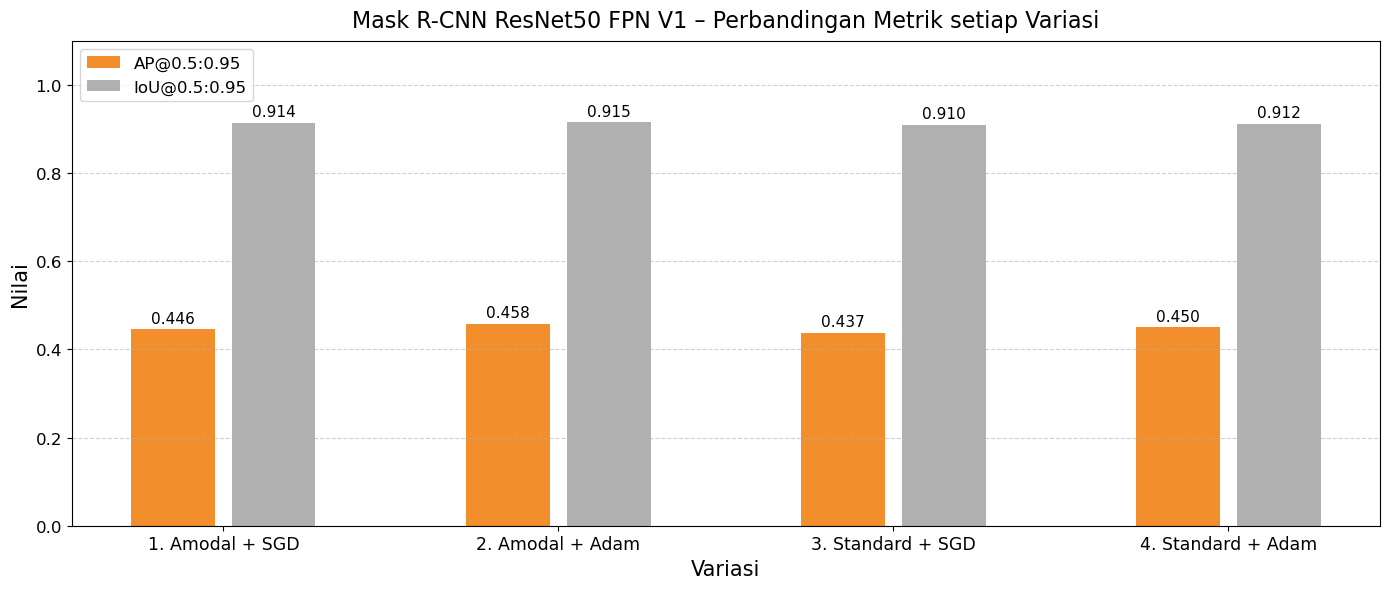
\includegraphics[width=1\textwidth]{figure/v1-version2d.png}
    \caption{Hasil Evaluasi \textit{Mask} R-CNN ResNet50 FPN V1}
    \label{fig:4.hasil_evaluasi_model_v1}
\end{figure}

Berdasarkan Tabel \ref{table:4.hasil_evaluasi_model_v1} dan Gambar \ref{fig:4.hasil_evaluasi_model_v1}, hasil evaluasi menggunakan metode \textit{K-Fold Cross Validation} menunjukkan bahwa variasi model \textit{Amodal} dengan \textit{optimizer} \textit{Adam} (variasi ke-2) menghasilkan performa rata-rata terbaik, dengan nilai \textit{AP50:95} sebesar 0{,}458 dan \textit{IoU50:95} sebesar 0{,}915. Secara spesifik, model terbaik diperoleh pada \textit{fold} pertama dengan capaian nilai \textit{AP50:95} mencapai 0{,}487 dengan \textit{IoU50:95} sebesar 0{,}915. Meskipun demikian, nilai \textit{IoU50:95} tertinggi justru diraih oleh variasi model \textit{Amodal} dengan \textit{optimizer} SGD (variasi ke-1), yaitu sebesar 0{,}919 pada \textit{fold} ke-4, meskipun dengan nilai \textit{AP50:95} yang sedikit lebih rendah, yaitu 0{,}449. \par

\subsection{Hasil Evaluasi \textit{Mask} R-CNN ResNet50 FPN V2}
Hasil evaluasi \textit{Model Pre-trained} \textit{Mask} R-CNN ResNet50 FPN V2 dengan variasi konfigurasi pelatihan dan dihitung metrik AP dan IoU ditampilkan pada Tabel \ref{table:4.hasil_evaluasi_model_v2}.

\begin{table}[H]
\centering
\caption{Hasil Evaluasi \textit{Mask} R-CNN ResNet50 FPN V2}
\label{table:4.hasil_evaluasi_model_v2}
% \footnotesize
\small
% \setlength{\tabcolsep}{6pt} % Menyesuaikan jarak antar kolom agar lebih ramping
\makebox[\textwidth][c]{
\begin{tabular}{|c|c|c|c|c|c|c|c|c|c|}
\hline
\multirow{2}{*}{\textbf{No}} & \multirow{2}{*}{\textbf{Model}} & \multirow{2}{*}{\textbf{Optim}} & \multirow{2}{*}{\textbf{Fold}} & \multicolumn{3}{c|}{\textbf{AP}} & \multicolumn{3}{c|}{\textbf{IoU}} \\
\cline{5-10}
& & & & \textbf{0.5} & \textbf{0.75} & \textbf{0.5:0.95} & \textbf{0.5} & \textbf{0.75} & \textbf{0.5:0.95} \\
\hline
\multirow{6}{*}{1} & \multirow{6}{*}{\textit{Amodal}} & \multirow{6}{*}{SGD} & 1 & 0{,}524 & 0{,}474 & 0{,}421 & 0{,}882 & 0{,}910 & 0{,}911 \\
\cline{4-10}
& & & 2 & 0{,}486 & 0{,}443 & 0{,}386 & 0{,}883 & 0{,}905 & 0{,}908 \\
\cline{4-10}
& & & 3 & 0{,}510 & 0{,}469 & 0{,}412 & 0{,}888 & 0{,}909 & 0{,}913 \\
\cline{4-10}
& & & 4 & 0{,}495 & 0{,}453 & 0{,}404 & 0{,}897 & 0{,}916 & 0{,}919 \\
\cline{4-10}
& & & 5 & 0{,}478 & 0{,}438 & 0{,}382 & 0{,}881 & 0{,}903 & 0{,}907 \\
\cline{4-10}
& & & Avg & 0{,}499 & 0{,}455 & 0{,}401 & 0{,}886 & 0{,}909 & 0{,}912 \\
\hline
\multirow{6}{*}{2} & \multirow{6}{*}{\textit{Amodal}} & \multirow{6}{*}{\textit{Adam}} & 1 & 0{,}545 & 0{,}509 & 0{,}447 & 0{,}893 & 0{,}912 & 0{,}915 \\
\cline{4-10}
& & & 2 & 0{,}524 & 0{,}481 & 0{,}424 & 0{,}892 & 0{,}910 & 0{,}913 \\
\cline{4-10}
& & & 3 & 0{,}503 & 0{,}456 & 0{,}405 & 0{,}888 & 0{,}909 & 0{,}912 \\
\cline{4-10}
& & & 4 & 0{,}504 & 0{,}466 & 0{,}408 & 0{,}888 & 0{,}908 & 0{,}911 \\
\cline{4-10}
& & & 5 & 0{,}510 & 0{,}473 & 0{,}417 & 0{,}889 & 0{,}908 & 0{,}912 \\
\cline{4-10}
& & & Avg & 0{,}517 & 0{,}477 & 0{,}420 & 0{,}890 & 0{,}909 & 0{,}913 \\
\hline
\multirow{6}{*}{3} & \multirow{6}{*}{\textit{Standard}} & \multirow{6}{*}{SGD} & 1 & 0{,}574 & 0{,}530 & \textbf{0{,}472} & 0{,}894 & 0{,}914 & 0{,}916 \\
\cline{4-10}
& & & 2 & 0{,}550 & 0{,}510 & 0{,}442 & 0{,}886 & 0{,}905 & 0{,}909 \\
\cline{4-10}
& & & 3 & 0{,}541 & 0{,}504 & 0{,}453 & 0{,}893 & 0{,}914 & 0{,}917 \\
\cline{4-10}
& & & 4 & 0{,}543 & 0{,}503 & 0{,}448 & 0{,}898 & 0{,}914 & 0{,}917 \\
\cline{4-10}
& & & 5 & 0{,}526 & 0{,}484 & 0{,}428 & 0{,}891 & 0{,}909 & 0{,}914 \\
\cline{4-10}
& & & \cellcolor{black!15}Avg & 0{,}547 & 0{,}506 & \cellcolor{black!15}\textbf{0{,}449} & 0{,}892 & 0{,}911 & \cellcolor{black!15}\textbf{0{,}915} \\
\hline
\multirow{6}{*}{4} & \multirow{6}{*}{\textit{Standard}} & \multirow{6}{*}{\textit{Adam}} & 1 & 0{,}568 & 0{,}525 & 0{,}463 & 0{,}891 & 0{,}912 & 0{,}914 \\
\cline{4-10}
& & & 2 & 0{,}550 & 0{,}511 & 0{,}444 & 0{,}886 & 0{,}906 & 0{,}909 \\
\cline{4-10}
& & & 3 & 0{,}534 & 0{,}490 & 0{,}437 & 0{,}892 & 0{,}910 & 0{,}914 \\
\cline{4-10}
& & & 4 & 0{,}542 & 0{,}507 & 0{,}454 & 0{,}900 & 0{,}918 & \textbf{0{,}921} \\
\cline{4-10}
& & & 5 & 0{,}550 & 0{,}505 & 0{,}443 & 0{,}892 & 0{,}911 & 0{,}915 \\
\cline{4-10}
& & & Avg & 0{,}547 & 0{,}506 & 0{,}448 & 0{,}892 & 0{,}912 & 0{,}914 \\
\hline
\end{tabular}
}
\end{table}

Visualisasi dari hasil evaluasi \textit{Mask} R-CNN ResNet50 FPN V2 ditampilkan pada Gambar \ref{fig:4.hasil_evaluasi_model_v2}.

\begin{figure}[H] % Kalau menggunakan H, posisi gambar akan tepat dibawah teks
    \centering
    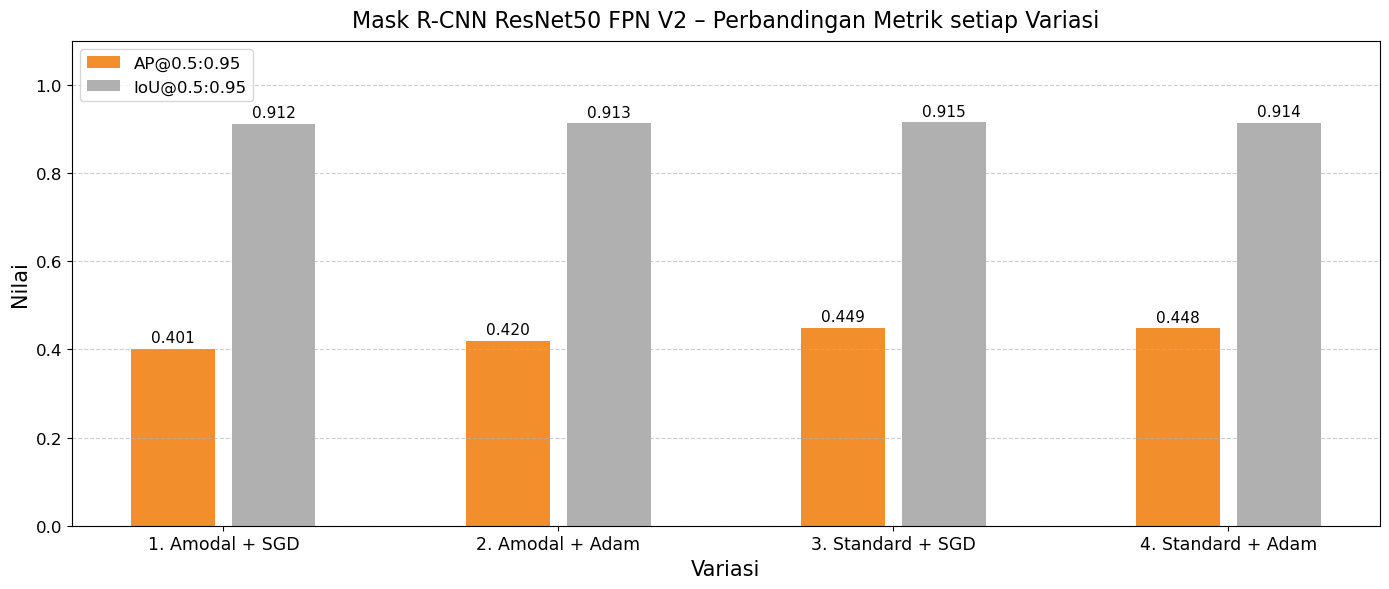
\includegraphics[width=1\textwidth]{figure/v2-version2d.png}
    \caption{Hasil Evaluasi \textit{Mask} R-CNN ResNet50 FPN V2}
    \label{fig:4.hasil_evaluasi_model_v2}
\end{figure}

Berdasarkan Tabel \ref{table:4.hasil_evaluasi_model_v2} dan Gambar \ref{fig:4.hasil_evaluasi_model_v2}, hasil evaluasi menggunakan metode \textit{K-Fold Cross Validation} menunjukkan bahwa variasi model \textit{Standard} dengan \textit{optimizer} SGD (variasi ke-3) menghasilkan performa rata-rata terbaik, dengan nilai \textit{AP50:95} sebesar 0{,}449 dan \textit{IoU50:95} sebesar 0{,}915. Secara spesifik, model terbaik diperoleh pada \textit{fold} pertama dengan capaian nilai \textit{AP50:95} mencapai 0{,}472 dengan \textit{IoU50:95} sebesar 0{,}916. Meskipun demikian, nilai \textit{IoU50:95} tertinggi justru dicapai oleh variasi model \textit{Standard} dengan \textit{optimizer} \textit{Adam} (variasi ke-4), yaitu sebesar 0{,}921 pada \textit{fold} ke-4, meskipun dengan nilai \textit{AP50:95} yang sedikit lebih rendah, yaitu 0{,}454. \par

\section{Perbandingan Evaluasi Model} \label{IV.Perbandingan_Evaluasi_Model}
Hasil pertimbangan dari kedua model \textit{pre-trained} berdasarkan variasi konfigurasi pelatihan dengan performa terbaik berdasarkan rata-rata metrik \textit{AP50:95} dari hasil metode \textit{K-Fold Cross Validation} yang ditampilkan pada Tabel \ref{table:4.perbandingan_evaluasi_model}.

\begin{table}[H]
\centering
\caption{Hasil Perbandingan Evaluasi Model Terbaik}
\label{table:4.perbandingan_evaluasi_model}
\small
\makebox[\textwidth][c]{
\begin{tabular}{|c|c|c|c|c|}
\hline
\multirow{2}{*}{\textbf{Model \textit{Pre-trained}}} & \multirow{2}{*}{\textbf{Model}} & \multirow{2}{*}{\textbf{Optimizer}} & \textbf{AP} & \textbf{IoU} \\
\cline{4-5}
& & & \textbf{0.5:0.95} & \textbf{0.5:0.95} \\
\hline
\textbf{\textit{Mask} R-CNN ResNet50 FPN V1} & \textbf{\textit{Amodal}} & \textbf{\textit{Adam}} & \textbf{0{,}458} & \textbf{0{,}915} \\
\hline
\textit{Mask} R-CNN ResNet50 FPN V1 & \textit{Standard} & SGD & 0{,}437 & 0{,}910 \\
\hline
\textit{Mask} R-CNN ResNet50 FPN V2 & \textit{Amodal} & \textit{Adam} & 0{,}420 & 0{,}913 \\
\hline
\textbf{\textit{Mask} R-CNN ResNet50 FPN V2} & \textbf{\textit{Standard}} & \textbf{SGD} & \textbf{0{,}449} & \textbf{0{,}915} \\
\hline
\end{tabular}
}
\end{table}

Berdasarkan Tabel \ref{table:4.perbandingan_evaluasi_model}, dapat dilihat bahwa hasil perbandingan dua model terbaik didapatkan bahwa model \textit{pre-trained} \textit{Mask} R-CNN ResNet50 FPN V1 dengan variasi model \textit{Amodal} dan \textit{optimizer} \textit{Adam} menunjukkan performa terbaik dengan nilai \textit{AP50:95} sebesar 0{,}458 dan \textit{IoU50:95} sebesar 0{,}915. Model \textit{pre-trained} \textit{Mask} R-CNN ResNet50 FPN V2 dengan variasi model \textit{Standard} dan \textit{optimizer} SGD menunjukkan performa yang sedikit lebih rendah dengan nilai \textit{AP50:95} sebesar 0{,}449 dan \textit{IoU50:95} sebesar 0{,}915. \par

Performa unggul model dengan \textit{optimizer} \textit{Adam} dapat dilihat secara konsisten pada hasil evaluasi. Berdasarkan Tabel \ref{table:4.hasil_evaluasi_model_v1} untuk model V1 dan Tabel \ref{table:4.hasil_evaluasi_model_v2} untuk model V2, penggunaan \textit{optimizer} \textit{Adam} menghasilkan nilai \textit{AP50:95} yang lebih tinggi dibandingkan dengan \textit{optimizer} SGD. Keunggulan ini disebabkan oleh mekanisme \textit{adaptive learning rate} yang dimiliki \textit{Adam}, yang mampu mempercepat dan menstabilkan proses konvergensi, terutama pada objek dengan bentuk kompleks seperti citra mikroskop mineral kasiterit \cite{optimizer}. Sifat adaptif ini menjadikan \textit{Adam} lebih efektif untuk pendekatan \textit{amodal} yang memerlukan kemampuan prediksi lebih kompleks. Sementara itu, \textit{optimizer} SGD tetap menunjukkan stabilitas yang baik dalam proses pembelajaran pada pendekatan segmentasi standar, meskipun nilai \textit{AP50:95} yang dihasilkan sedikit lebih rendah, dengan selisih 0{,}009 dibandingkan model \textit{pre-trained Mask R-CNN ResNet50 FPN V2} dengan variasi model \textit{Standard} dan \textit{optimizer} SGD. Berdasarkan hasil evaluasi tersebut, dapat disimpulkan bahwa konfigurasi terbaik dalam penelitian ini adalah model \textit{pre-trained Mask R-CNN ResNet50 FPN V1} dengan variasi model \textit{Amodal} dan \textit{optimizer} \textit{Adam}. \par

\begin{table}[H]
\centering
\caption{Hasil Perbandingan Penerapan Amodal}
\label{table:4.perbandingan_penerapan_amodal}
\small
\makebox[\textwidth][c]{
\begin{tabular}{|c|c|c|c|c|c|c|}
\hline
\multirow{2}{*}{\textbf{Model \textit{Pre-trained}}} & \multirow{2}{*}{\textbf{Model}} & \multirow{2}{*}{\textbf{Optimizer}} & \multirow{2}{*}{\textbf{Parameter}} & \textbf{AP} & \textbf{IoU} & \multirow{2}{*}{\textbf{Waktu \textit{Train}}} \\
\cline{5-6}
& & & & \textbf{0.5:0.95} & \textbf{0.5:0.95} & \\
\hline
\textbf{\textit{Mask} R-CNN V1} & \textbf{\textit{Amodal}} & \textbf{\textit{Adam}} & \textbf{46,650,909} & \textbf{0{,}458} & \textbf{0{,}915} & \textbf{4.46 jam} \\
\hline
\textit{Mask} R-CNN V1 & \textit{Standard} & SGD & 43,699,995  & 0{,}437 & 0{,}910 & 4.09 jam \\
\hline
\textit{Mask} R-CNN V2 & \textit{Amodal} & \textit{Adam} & 48,605,981 & 0{,}420 & 0{,}913 & 4.14 jam \\
\hline
\textbf{\textit{Mask} R-CNN V2} & \textbf{\textit{Standard}} & \textbf{SGD} & \textbf{45,655,067} & \textbf{0{,}449} & \textbf{0{,}915} & \textbf{3.69 jam} \\
\hline
\end{tabular}
}
\end{table}

Berdasarkan Tabel \ref{table:4.perbandingan_penerapan_amodal}, penerapan teknik \textit{Amodal Instance Segmentation} menunjukkan pengaruh yang berbeda pada masing-masing model \textit{pre-trained} \textit{Mask} R-CNN yang diuji. Pada model \textit{pre-trained} \textit{Mask} R-CNN ResNet50 FPN V1 dengan \textit{optimizer} \textit{Adam}, penambahan teknik \textit{amodal} yang meningkatkan jumlah parameter sebesar 2{,}950{,}914 (sekitar 6{,}75\%) menghasilkan peningkatan performa, ditunjukkan oleh kenaikan nilai \textit{AP50:95} sebesar 0{,}021 (dari 0{,}437 menjadi 0{,}458) serta peningkatan \textit{IoU50:95} sebesar 0{,}005 (dari 0{,}910 menjadi 0{,}915). Peningkatan ini disertai dengan penambahan waktu pelatihan sebesar 0{,}37 jam, yang masih berada dalam batas komputasi yang dapat diterima untuk skenario segmentasi objek dengan tingkat oklusi tinggi.

Sebaliknya, pada model \textit{pre-trained} \textit{Mask} R-CNN ResNet50 FPN V2 dengan \textit{optimizer} SGD, penerapan teknik \textit{amodal}  yang meningkatkan jumlah parameter sebesar 2{,}950{,}914 (sekitar 6{,}46\%) tidak memberikan peningkatan performa. Nilai \textit{AP50:95} justru mengalami penurunan sebesar 0{,}029 (dari 0{,}449 menjadi 0{,}420), sementara nilai \textit{IoU50:95} menurun sebesar 0{,}002 (dari 0{,}915 menjadi 0{,}913), meskipun waktu pelatihan hanya bertambah 0{,}45 jam. Hasil ini menunjukkan bahwa penambahan kompleksitas model melalui pendekatan \textit{amodal} tidak selalu berbanding lurus dengan peningkatan kinerja, serta mengindikasikan bahwa efektivitas penerapan teknik \textit{Amodal Instance Segmentation} sangat bergantung pada kesesuaian dengan model \textit{pre-trained} dan pemilihan \textit{optimizer} yang digunakan.

\begin{table}[H]
\centering
\caption{Hasil Perbandingan Evaluasi Model Terbaik per Parameter}
\label{table:4.perbandingan_parameter_model}
\small
\makebox[\textwidth][c]{
\begin{tabular}{|c|c|c|c|c|c|c|}
\hline
\multirow{2}{*}{\parbox{2.5cm}{\centering\textbf{Model \textit{Pre-trained}}}} & \multirow{2}{*}{\textbf{Model}} & \multirow{2}{*}{\textbf{Optim}} & \multirow{2}{*}{\textbf{Parameter}} & \multirow{2}{*}{\parbox{1.1cm}{\centering\textbf{Param Ratio}}} & \multicolumn{2}{c|}{\textbf{Perbandingan (Metrik/Param)}} \\
\cline{6-7}
& & & & & \parbox{1.85cm}{\centering\textbf{AP/Param}} & \textbf{IoU/Param} \\
\hline
\textit{Mask} R-CNN V1 & \textit{Amodal} & \textit{Adam} & 46,650,909 & 1{,}067$\times$ & 9{,}814e-9 & 1{,}962e-8 \\
\hline
\textbf{\textit{Mask} R-CNN V1} & \textbf{\textit{Standard}} & \textbf{SGD} & \textbf{43,699,995} & \textbf{1{,}000$\times$} & \textbf{9{,}999e-9} & \textbf{2{,}082e-8} \\
\hline
\textit{Mask} R-CNN V2 & \textit{Amodal} & \textit{Adam} & 48,605,981 & 1{,}113$\times$ & 8{,}644e-9 & 1{,}878e-8 \\
\hline
\textbf{\textit{Mask} R-CNN V2} & \textbf{\textit{Standard}} & \textbf{SGD} & \textbf{45,655,067} & \textbf{1{,}045$\times$} & \textbf{9{,}835e-9} & \textbf{2{,}004e-8} \\
\hline
\end{tabular}
}
\end{table}

Berdasarkan Tabel \ref{table:4.perbandingan_parameter_model}, evaluasi efisiensi parameter menunjukkan perbedaan kemampuan tiap model dalam memanfaatkan kompleksitas model terhadap kinerja yang dihasilkan. Model \textit{Mask} R-CNN ResNet50 FPN V1 \textit{Standard} dengan \textit{optimizer} SGD digunakan sebagai \textit{baseline} (\textit{Param Ratio} 1{,}000$\times$) dengan total 43.699.995 parameter dan menunjukkan efisiensi parameter tertinggi, ditunjukkan oleh rasio \textit{AP/Param} sebesar 9{,}999e-9 dan \textit{IoU/Param} sebesar 2{,}082e-8. Penerapan teknik \textit{amodal} pada model \textit{Mask} R-CNN V1 meningkatkan jumlah parameter menjadi 46.650.909 (\textit{Param Ratio} 1{,}067$\times$), namun tidak diikuti oleh peningkatan efisiensi, karena nilai \textit{AP/Param} dan \textit{IoU/Param} justru lebih rendah dibandingkan versi \textit{Standard}. \par

Hal yang sama juga terlihat pada model \textit{Mask} R-CNN ResNet50 FPN V2. Model \textit{Standard} dengan \textit{optimizer} SGD (\textit{Param Ratio} 1{,}045$\times$) menunjukkan rasio \textit{AP/Param} dan \textit{IoU/Param} yang lebih seimbang dibandingkan model V2 \textit{Amodal} (\textit{Param Ratio} 1{,}113$\times$). Meskipun model V1 \textit{Standard} \textit{optimizer} dengan SGD memiliki efisiensi parameter tertinggi, model V2 \textit{Standard} \textit{optimizer} dengan SGD merepresentasikan keseimbangan yang lebih baik antara kompleksitas model, efisiensi parameter, dan performa deteksi, sehingga lebih sesuai untuk penerapan praktis pada segmentasi mineral kasiterit. Secara keseluruhan, hasil ini menunjukkan bahwa peningkatan jumlah parameter melalui pendekatan \textit{amodal} tidak selalu berbanding lurus dengan peningkatan efisiensi model. \par


\section{Pengujian Model} \label{IV.Pengujian_Model}
Pengujian model akan di lakukan menggunakan ke dua model terbaik yang telah di dapatkan dari hasil evaluasi pada Bagian \ref{IV.Perbandingan_Evaluasi_Model}, yaitu model \textit{pre-trained} \textit{Mask} R-CNN ResNet50 FPN V1 dengan variasi model \textit{Amodal} dan \textit{optimizer} \textit{Adam} (V1 \textit{Am}) serta model \textit{pre-trained} \textit{Mask} R-CNN ResNet50 FPN V2 dengan variasi model \textit{Standard} dan \textit{optimizer} SGD (V2 \textit{Std}). Pengujian dilakukan pada 6 citra uji yang berbeda dari dataset pelatihan. Hasil pengujian ditampilkan pada Tabel \ref{table:4.Pengujian1}. Evaluasi kinerja prediksi dilakukan berdasarkan beberapa kategori evaluasi prediksi yang ditentukan dengan mempertimbangkan nilai \textit{Intersection over Union} (IoU) antara prediksi dan \textit{ground truth}, skor kepercayaan (\textit{confidence score}), serta kesesuaian label objek. Berdasarkan kriteria tersebut, hasil prediksi dikelompokkan ke dalam lima kategori, yaitu \textit{Correct}, \textit{Low Confidence}, \textit{Wrong Location}, \textit{False Positive}, dan \textit{False Negative}. 

Pada pengujian ini, evaluasi hasil prediksi model dilakukan dengan mengelompokkan setiap prediksi ke dalam beberapa kategori evaluasi prediksi berdasarkan nilai \textit{Intersection over Union} (IoU), skor kepercayaan (\textit{confidence score}), serta kesesuaian label prediksi terhadap \textit{ground truth}. Nilai ambang batas (\textit{threshold}) dan ambang batas IoU (\textit{IoU threshold}) ditetapkan sebesar 0,5 \cite{threshold_pengujian}, sedangkan ambang batas kepercayaan (\textit{confidence threshold}) ditetapkan sebesar 0,7. prediksi dikategorikan sebagai \textit{Correct} apabila memiliki nilai IoU $\geq 0,5$, skor kepercayaan $\geq 0,7$, dan label prediksi sesuai dengan \textit{ground truth}. Kategori \textit{Low Confidence} diberikan pada prediksi dengan IoU $\geq 0,5$ dan label yang benar, namun skor kepercayaan $<$ 0,7. Prediksi dengan label yang sesuai tetapi memiliki nilai IoU $<$ 0,5 diklasifikasikan sebagai \textit{Wrong Location}. Selanjutnya, \textit{False Positive} merupakan prediksi yang tidak memiliki pasangan \textit{ground truth} yang sesuai atau memiliki label yang tidak cocok, sedangkan \textit{False Negative} merupakan objek pada \textit{ground truth} yang tidak berhasil terprediksi oleh model.

% Atur margin untuk landscape - bisa disesuaikan nilai left dan right
\newgeometry{top=2cm, bottom=1.75cm, left=2cm, right=2cm}

\begin{landscape}
% \thispagestyle{landscape} % Untuk page number yang benar di landscape
\renewcommand{\arraystretch}{1.2} % Mengatur jarak antar baris tabel
\centering 
\begin{longtable}{|c|c|c|c|c|c|c|c|c|c|c|c|c|}
    \caption{Hasil Pengujian Model}
    \label{table:4.Pengujian1}\\
    \hline
    \multirow{2}{*}{\parbox{0.375cm}{\centering\textbf{No}}} & 
    \multirow{2}{*}{\parbox{4.0cm}{\centering\textbf{Citra}}} & 
    \multirow{2}{*}{\parbox{0.75cm}{\centering\textbf{GT\\Total}}} & 
    \multicolumn{8}{c|}{\textbf{Prediksi}} &
    \multirow{2}{*}{\parbox{1.2cm}{\centering\textbf{Hitung\\Manual}}} &
    \multirow{2}{*}{\parbox{1cm}{\centering\textbf{Model}}} \\
    \cline{4-11}
    & & &
    \parbox{0.75cm}{\centering\textbf{Total}} &
    \parbox{1.1cm}{\centering\textbf{Correct}} &
    \parbox{0.7cm}{\centering\textbf{\shortstack{Low\\[-0.2em]Conf}}} &
    \parbox{0.95cm}{\centering\textbf{\shortstack{Wrong\\[-0.35em]Loc}}} &
    \parbox{0.7cm}{\centering\textbf{\shortstack{False\\[-0.2em]Pos}}} &
    \parbox{0.7cm}{\centering\textbf{\shortstack{False\\[-0.2em]Neg}}} &
    \parbox{0.95cm}{\centering\textbf{\shortstack{AP\\[-0.2em]50:95}}} &
    \parbox{0.95cm}{\centering\textbf{\shortstack{IoU\\[-0.2em]50:95}}} &
    & \\

    \hline
    \endfirsthead
    
    \hline
    \multirow{2}{*}{\parbox{0.375cm}{\centering\textbf{No}}} & 
    \multirow{2}{*}{\parbox{4.0cm}{\centering\textbf{Citra}}} & 
    \multirow{2}{*}{\parbox{0.75cm}{\centering\textbf{GT\\Total}}} & 
    \multicolumn{8}{c|}{\textbf{Prediksi}} &
    \multirow{2}{*}{\parbox{1.2cm}{\centering\textbf{Hitung\\Manual}}} &
    \multirow{2}{*}{\parbox{1cm}{\centering\textbf{Model}}} \\
    \cline{4-11}
    & & &
    \parbox{0.75cm}{\centering\textbf{Total}} &
    \parbox{1.1cm}{\centering\textbf{Correct}} &
    \parbox{0.7cm}{\centering\textbf{\shortstack{Low\\[-0.2em]Conf}}} &
    \parbox{0.95cm}{\centering\textbf{\shortstack{Wrong\\[-0.35em]Loc}}} &
    \parbox{0.7cm}{\centering\textbf{\shortstack{False\\[-0.2em]Pos}}} &
    \parbox{0.7cm}{\centering\textbf{\shortstack{False\\[-0.2em]Neg}}} &
    \parbox{0.95cm}{\centering\textbf{\shortstack{AP\\[-0.2em]50:95}}} &
    \parbox{0.95cm}{\centering\textbf{\shortstack{IoU\\[-0.2em]50:95}}} &
    & \\
    \hline
    \endhead
    
    \hline
    \endfoot
    
    \hline
    \endlastfoot
    
    % ===== Data ke-1 =====
    \multirow{2}{*}{1} &
    \multirow{2}{*}{%
    \parbox[c][1.5cm][c]{4cm}{%
    \centering
    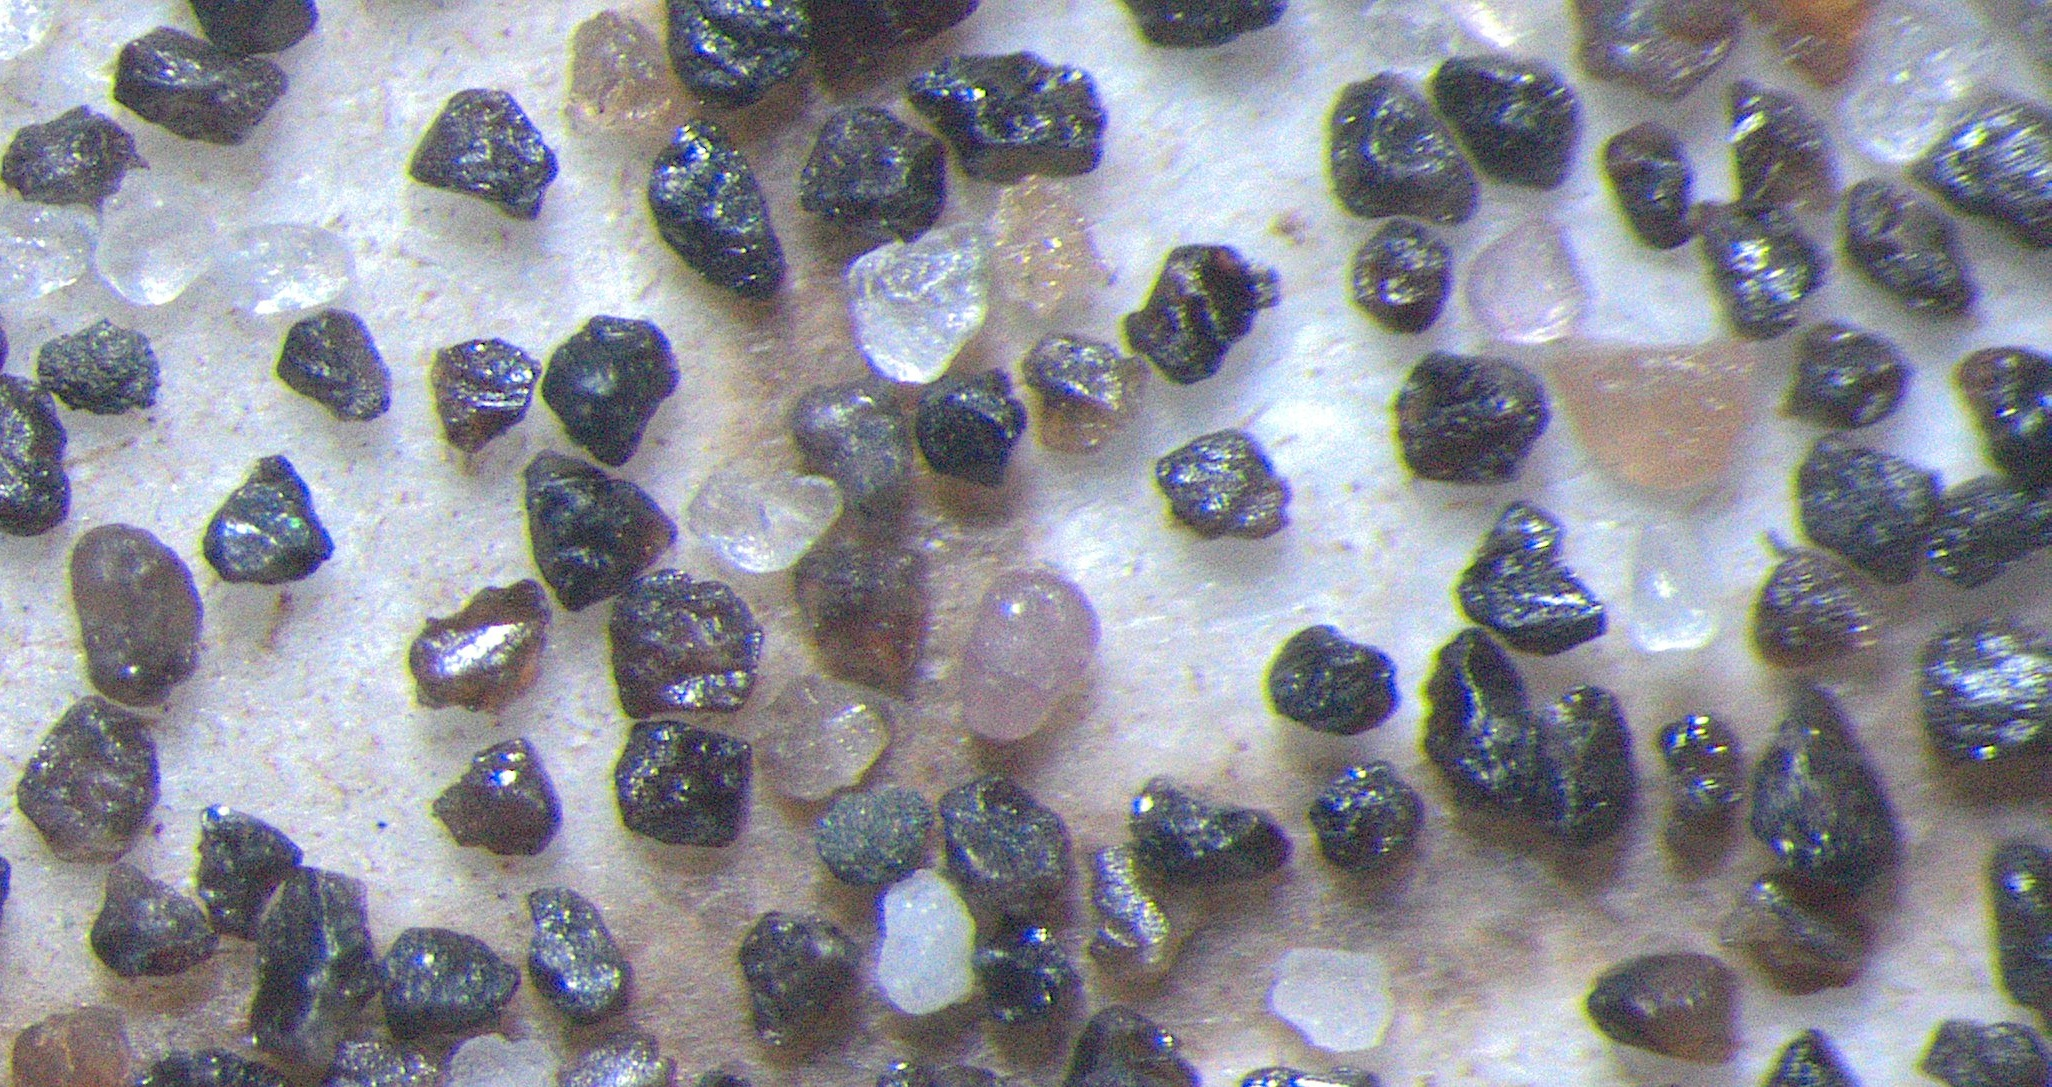
\includegraphics[width=4.05cm,height=4cm,keepaspectratio]{figure/pengujian/1/0384-16_100C_tile1.jpg}}} &
    \multirow{2}{*}{18} &

    34\rule{0pt}{3.0em} & 11 & 0 & 1 & 22 & 6 & 0{,}567 & 0{,}938 & 11 &
    V1 \textit{(Am)} \\

    \cline{4-13}

    & & &   % ← WAJIB: kosongkan No | Citra | GT Total
    36\rule{0pt}{3.0em} & 10 & 1 & 1 & 24 & 6 & 0{,}552 & 0{,}916 & 11 &
    V2 \textit{(Std)} \\

    \hline
    
    % ===== Data ke-2 =====
    \multirow{2}{*}{2} &
    \multirow{2}{*}{%
    \parbox[c][1.5cm][c]{4cm}{%
    \centering
    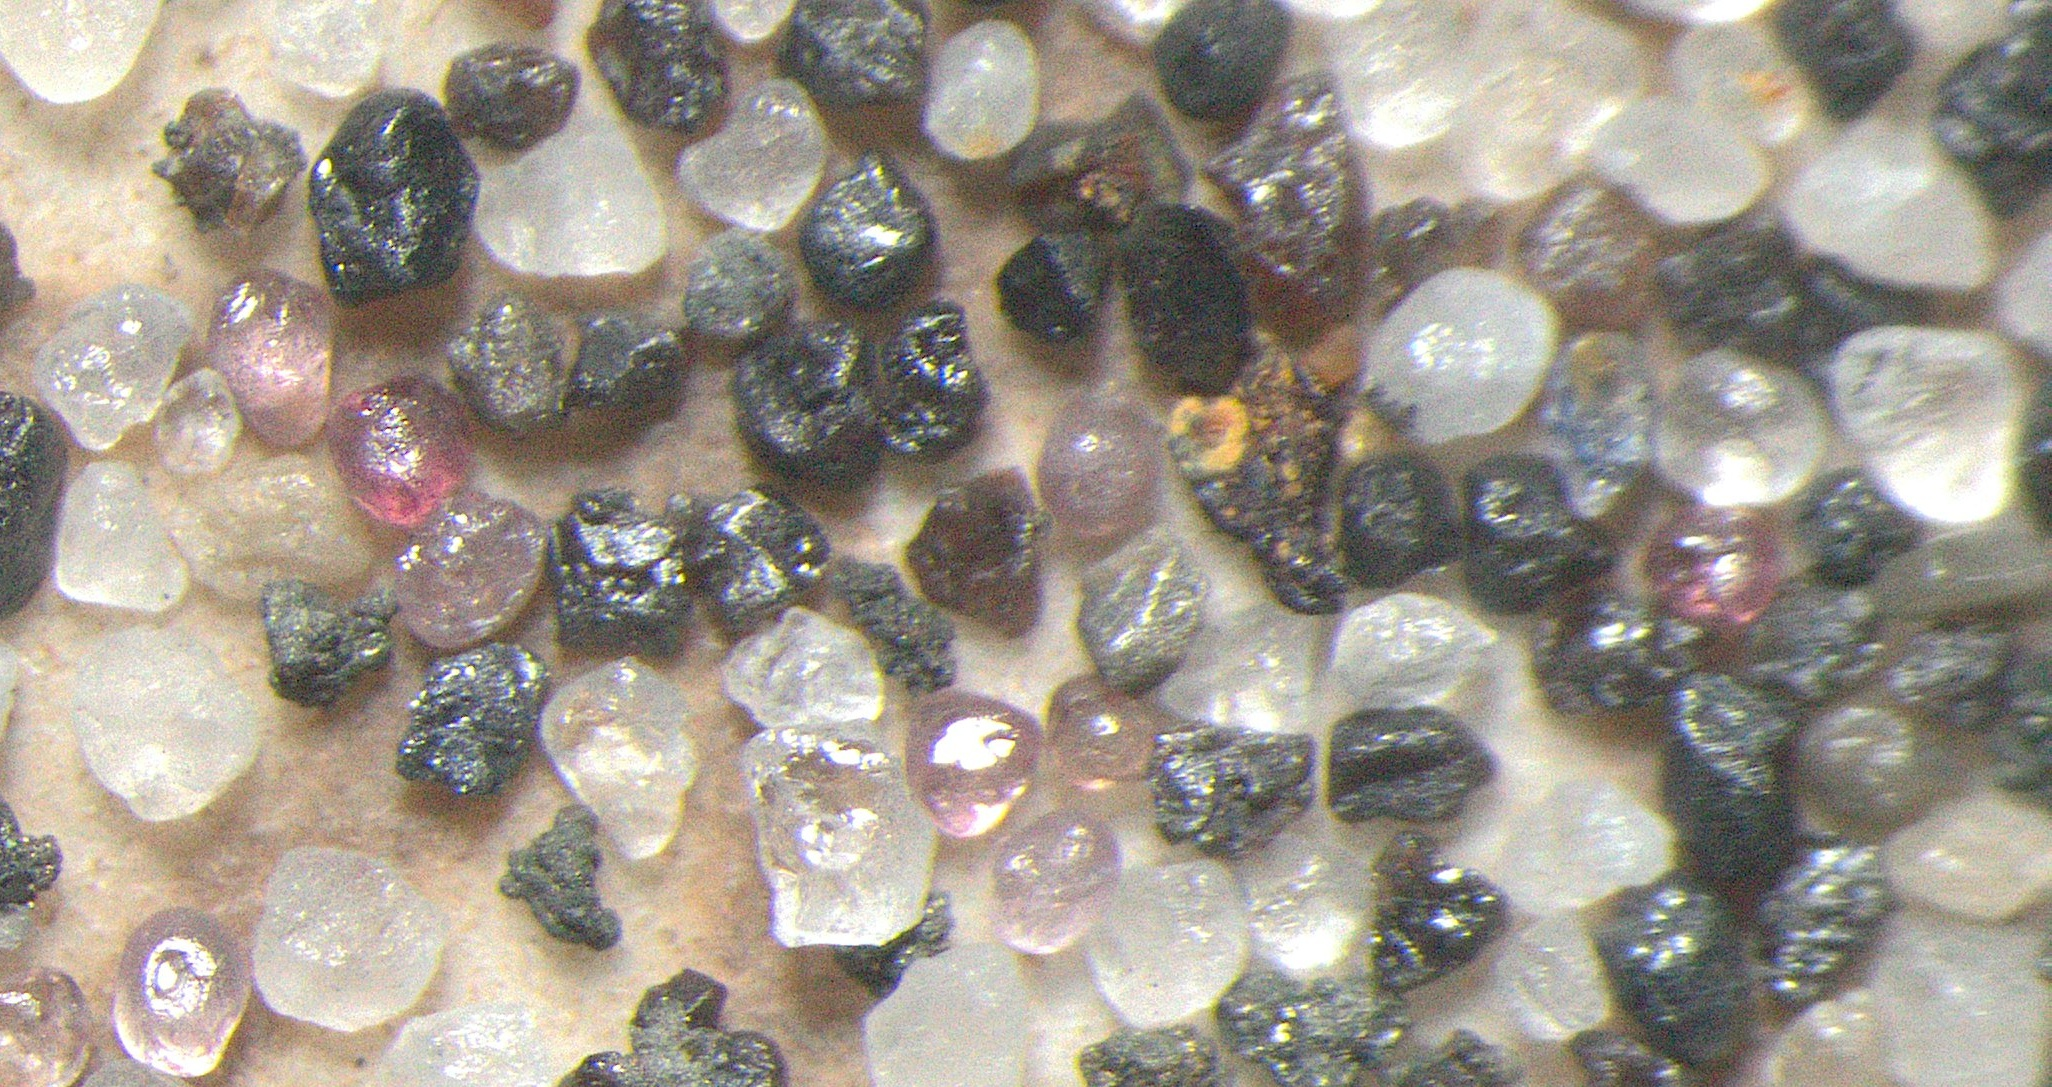
\includegraphics[width=4.05cm,height=4cm,keepaspectratio]{figure/pengujian/2/0384-16_48C_tile1.jpg}}} &
    \multirow{2}{*}{8} &

    16\rule{0pt}{3.0em} & 5 & 1 & 0 & 10 & 2 & 0{,}675 & 0{,}940 & 6 &
    V1 \textit{(Am)} \\

    \cline{4-13}

    & & &   % ← WAJIB: kosongkan No | Citra | GT Total
    28\rule{0pt}{3.0em} & 7 & 1 & 0 & 20 & 0 & 0{,}838 & 0{,}920 & 8 &
    V2 \textit{(Std)} \\

    \hline

    % ===== Data ke-3 =====
    \multirow{2}{*}{3} &
    \multirow{2}{*}{%
    \parbox[c][1.5cm][c]{4cm}{%
    \centering
    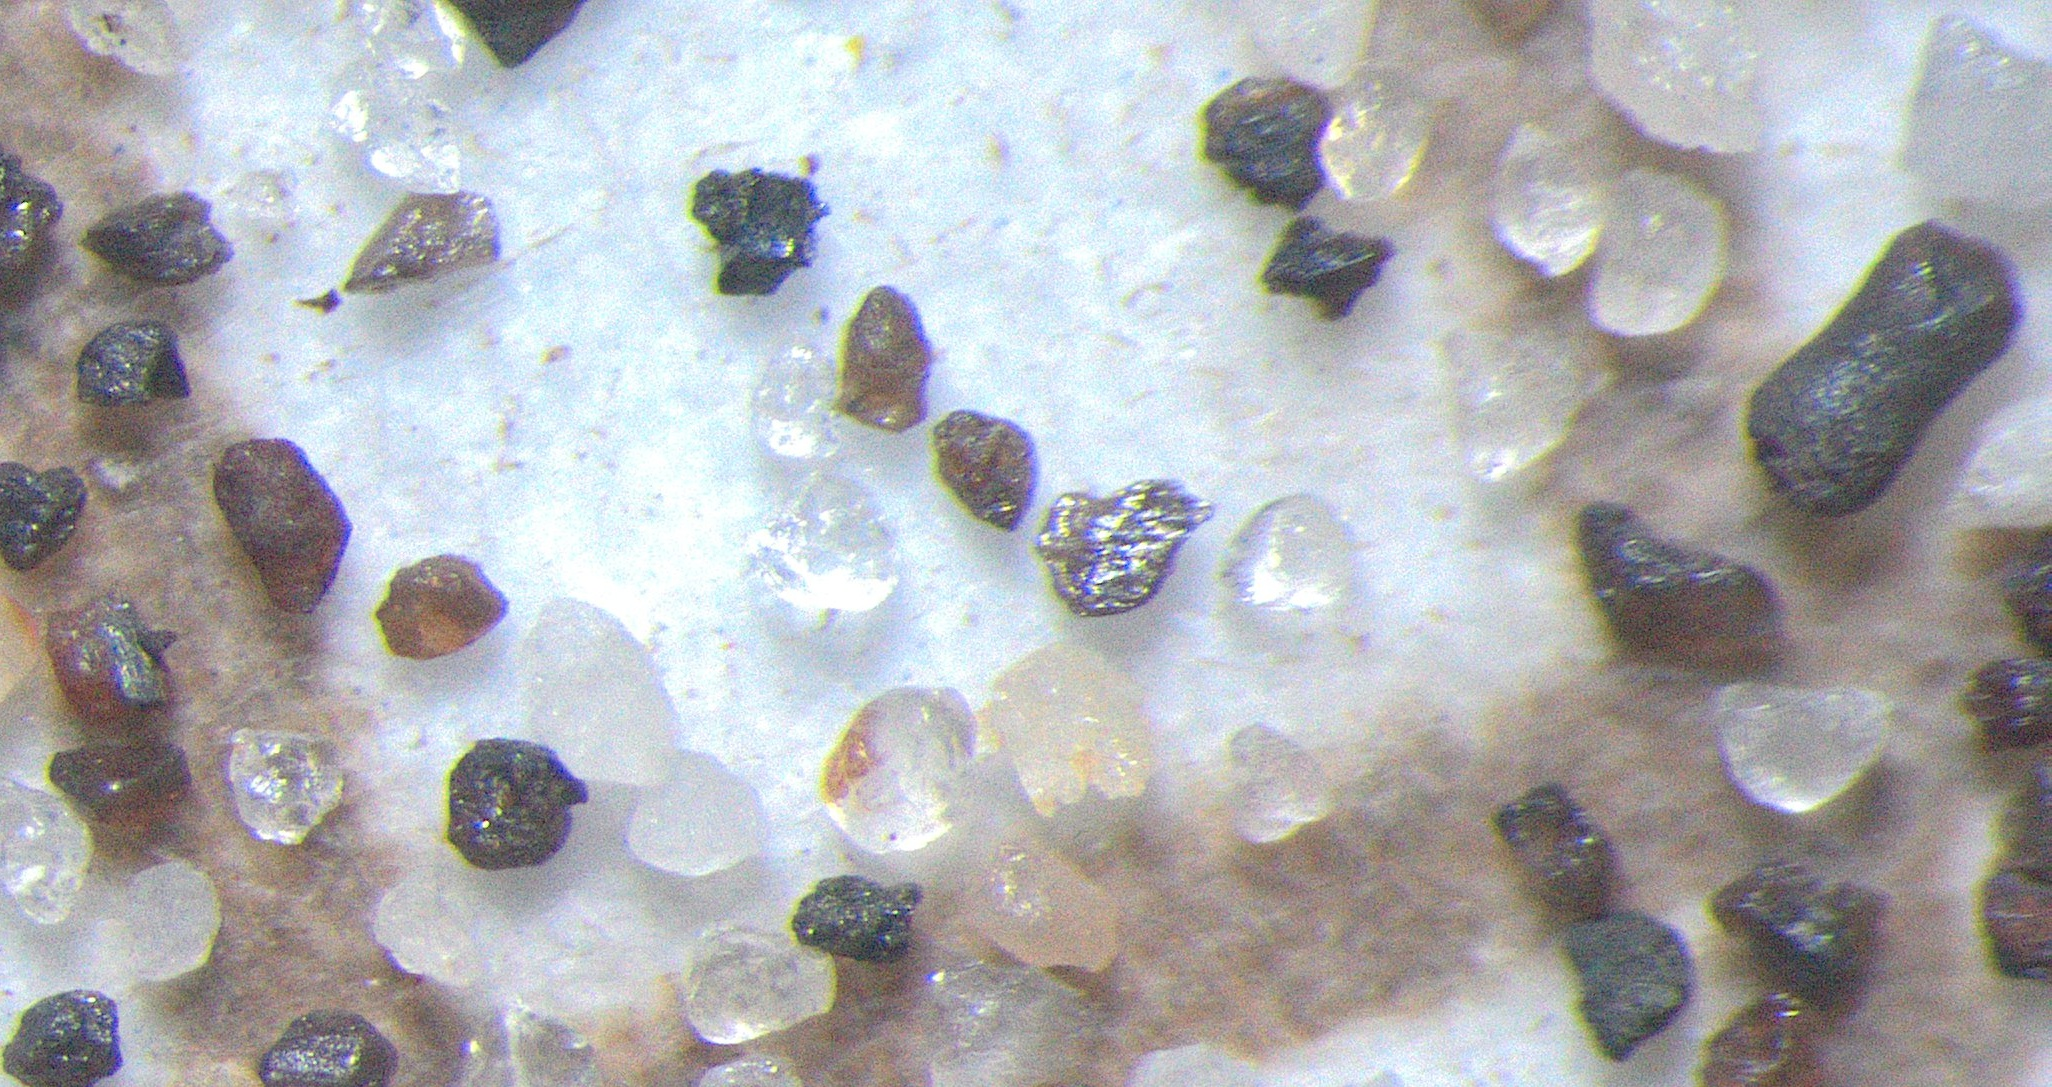
\includegraphics[width=4.05cm,height=4cm,keepaspectratio]{figure/pengujian/3/1347-20_100H_tile1.jpg}}} &
    \multirow{2}{*}{10} &

    21\rule{0pt}{3.0em} & 7 & 2 & 0 & 12 & 1 & 0{,}830 & 0{,}936 & 9 &
    V1 \textit{(Am)} \\

    \cline{4-13}

    & & &   % ← WAJIB: kosongkan No | Citra | GT Total
    19\rule{0pt}{3.0em} & 6 & 3 & 0 & 10 & 1 & 0{,}820 & 0{,}931 & 9 &
    V2 \textit{(Std)} \\

    \hline
\end{longtable}
\end{landscape}
\restoregeometry

    
\newgeometry{top=2cm, bottom=1.75cm, left=2cm, right=2cm}

\begin{landscape}
% \thispagestyle{landscape} % Untuk page number yang benar di landscape
\renewcommand{\arraystretch}{1.2} % Mengatur jarak antar baris tabel
\centering 
\begin{longtable}{|c|c|c|c|c|c|c|c|c|c|c|c|c|}
    % \caption{Hasil Pengujian Model}
    % \label{table:4.Pengujian4}\\
    \hline
    \multirow{2}{*}{\parbox{0.375cm}{\centering\textbf{No}}} & 
    \multirow{2}{*}{\parbox{4.0cm}{\centering\textbf{Citra}}} & 
    \multirow{2}{*}{\parbox{0.75cm}{\centering\textbf{GT\\Total}}} & 
    \multicolumn{8}{c|}{\textbf{Prediksi}} &
    \multirow{2}{*}{\parbox{1.2cm}{\centering\textbf{Hitung\\Manual}}} &
    \multirow{2}{*}{\parbox{0.85cm}{\centering\textbf{Model}}} \\
    \cline{4-11}
    & & &
    \parbox{0.75cm}{\centering\textbf{Total}} &
    \parbox{1.1cm}{\centering\textbf{Correct}} &
    \parbox{0.7cm}{\centering\textbf{\shortstack{Low\\[-0.2em]Conf}}} &
    \parbox{0.95cm}{\centering\textbf{\shortstack{Wrong\\[-0.35em]Loc}}} &
    \parbox{0.7cm}{\centering\textbf{\shortstack{False\\[-0.2em]Pos}}} &
    \parbox{0.7cm}{\centering\textbf{\shortstack{False\\[-0.2em]Neg}}} &
    \parbox{0.95cm}{\centering\textbf{\shortstack{AP\\[-0.2em]50:95}}} &
    \parbox{0.95cm}{\centering\textbf{\shortstack{IoU\\[-0.2em]50:95}}} &
    & \\

    \hline
    \endfirsthead
    
    \hline
    \multirow{2}{*}{\parbox{0.375cm}{\centering\textbf{No}}} & 
    \multirow{2}{*}{\parbox{4.0cm}{\centering\textbf{Citra}}} & 
    \multirow{2}{*}{\parbox{0.75cm}{\centering\textbf{GT\\Total}}} & 
    \multicolumn{8}{c|}{\textbf{Prediksi}} &
    \multirow{2}{*}{\parbox{1.2cm}{\centering\textbf{Hitung\\Manual}}} &
    \multirow{2}{*}{\parbox{0.85cm}{\centering\textbf{Model}}} \\
    \cline{4-11}
    & & &
    \parbox{0.75cm}{\centering\textbf{Total}} &
    \parbox{1.1cm}{\centering\textbf{Correct}} &
    \parbox{0.7cm}{\centering\textbf{\shortstack{Low\\[-0.2em]Conf}}} &
    \parbox{0.95cm}{\centering\textbf{\shortstack{Wrong\\[-0.35em]Loc}}} &
    \parbox{0.7cm}{\centering\textbf{\shortstack{False\\[-0.2em]Pos}}} &
    \parbox{0.7cm}{\centering\textbf{\shortstack{False\\[-0.2em]Neg}}} &
    \parbox{0.95cm}{\centering\textbf{\shortstack{AP\\[-0.2em]50:95}}} &
    \parbox{0.95cm}{\centering\textbf{\shortstack{IoU\\[-0.2em]50:95}}} &
    & \\
    \hline
    \endhead
    
    \hline
    \endfoot
    
    \hline
    \endlastfoot

    % ===== Data ke-4 =====
    \multirow{2}{*}{4} &
    \multirow{2}{*}{%
    \parbox[c][1.5cm][c]{4cm}{%
    \centering
    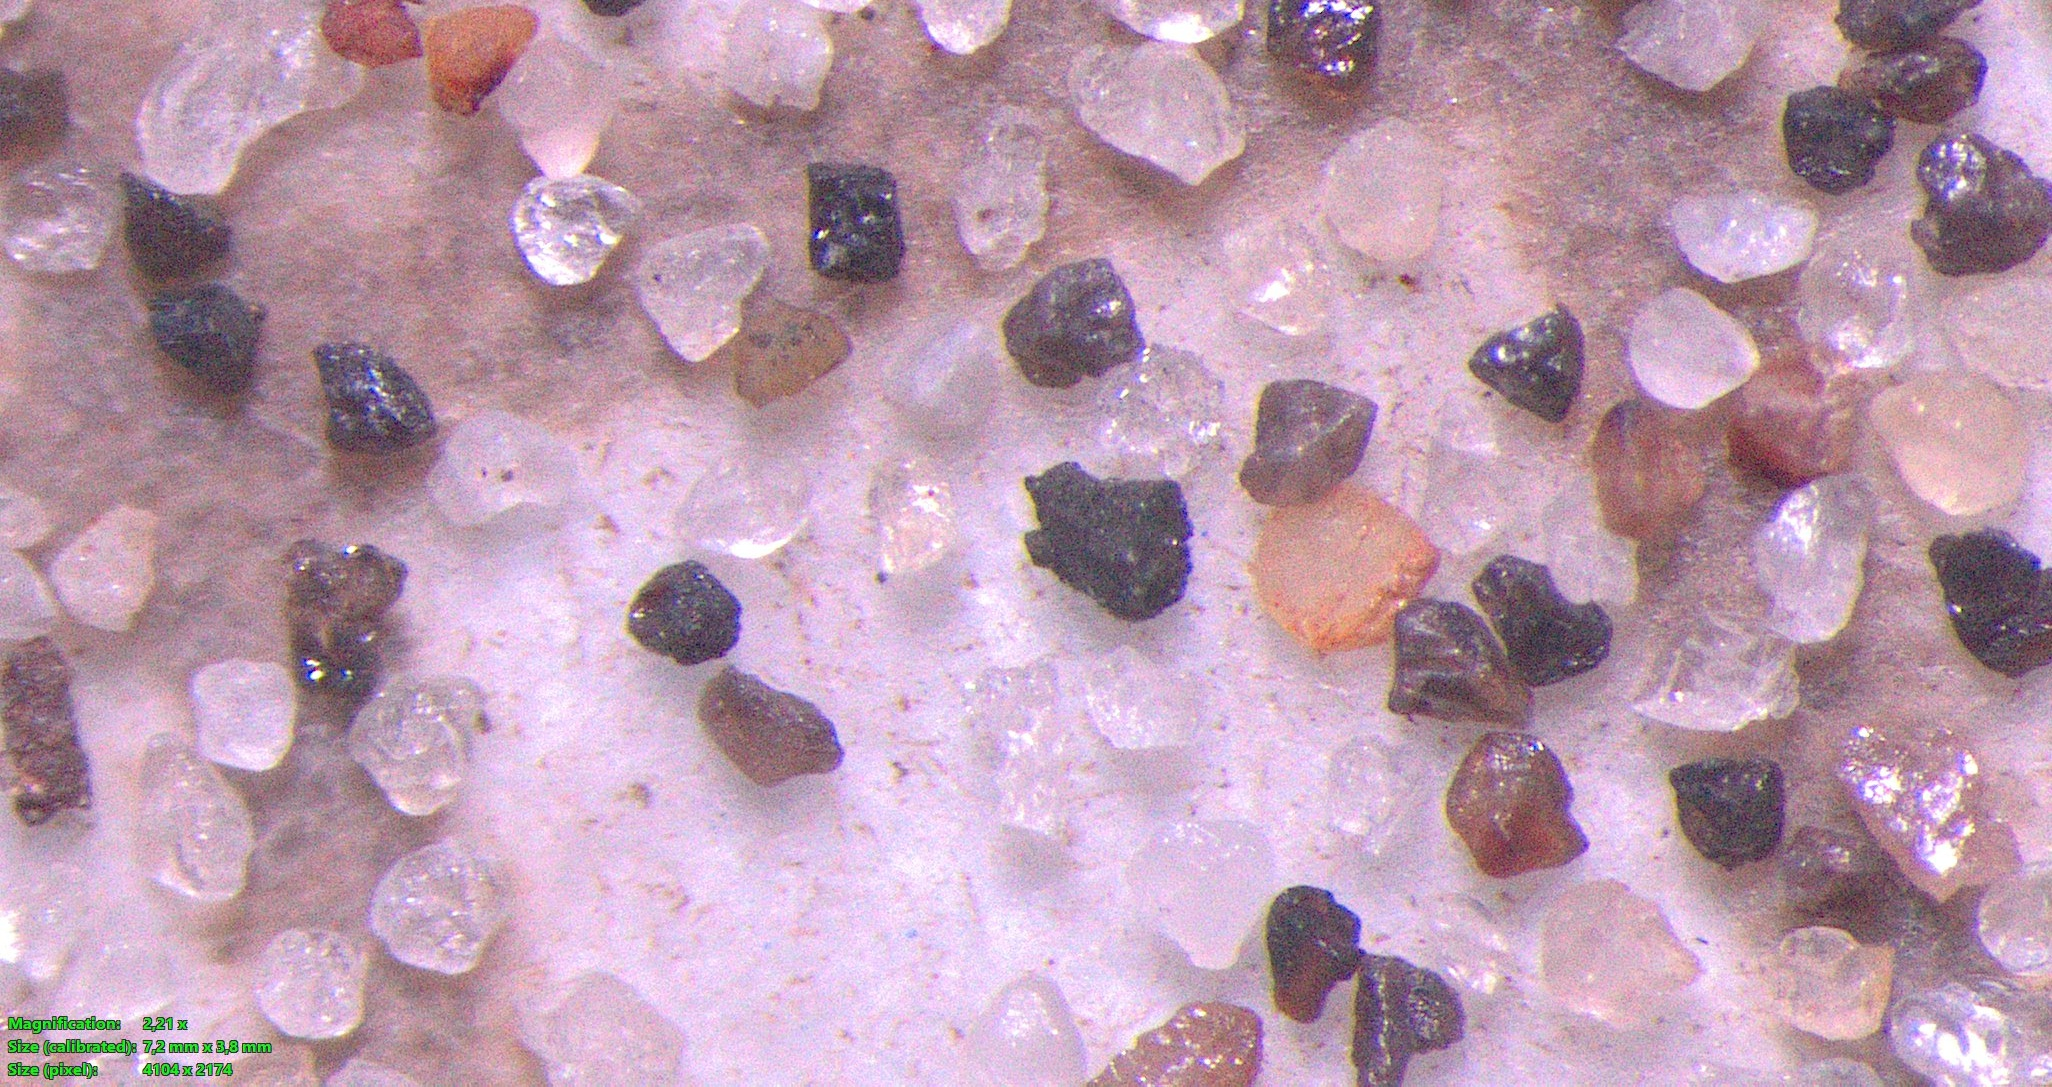
\includegraphics[width=4.05cm,height=4cm,keepaspectratio]{figure/pengujian/4/1347-17_100G_tile2.jpg}}} &
    \multirow{2}{*}{7} &

    12\rule{0pt}{3.0em} & 3 & 2 & 0 & 7 & 2 & 0{,}671 & 0{,}950 & 5 &
    V1 \textit{(Am)} \\

    \cline{4-13}

    & & &   % ← WAJIB: kosongkan No | Citra | GT Total
    21\rule{0pt}{3.0em} & 5 & 1 & 0 & 15 & 1 & 0{,}786 & 0{,}946 & 6 &
    V2 \textit{(Std)} \\

    \hline
    
    % ===== Data ke-5 =====
    \multirow{2}{*}{5} &
    \multirow{2}{*}{%
    \parbox[c][1.5cm][c]{4cm}{%
    \centering
    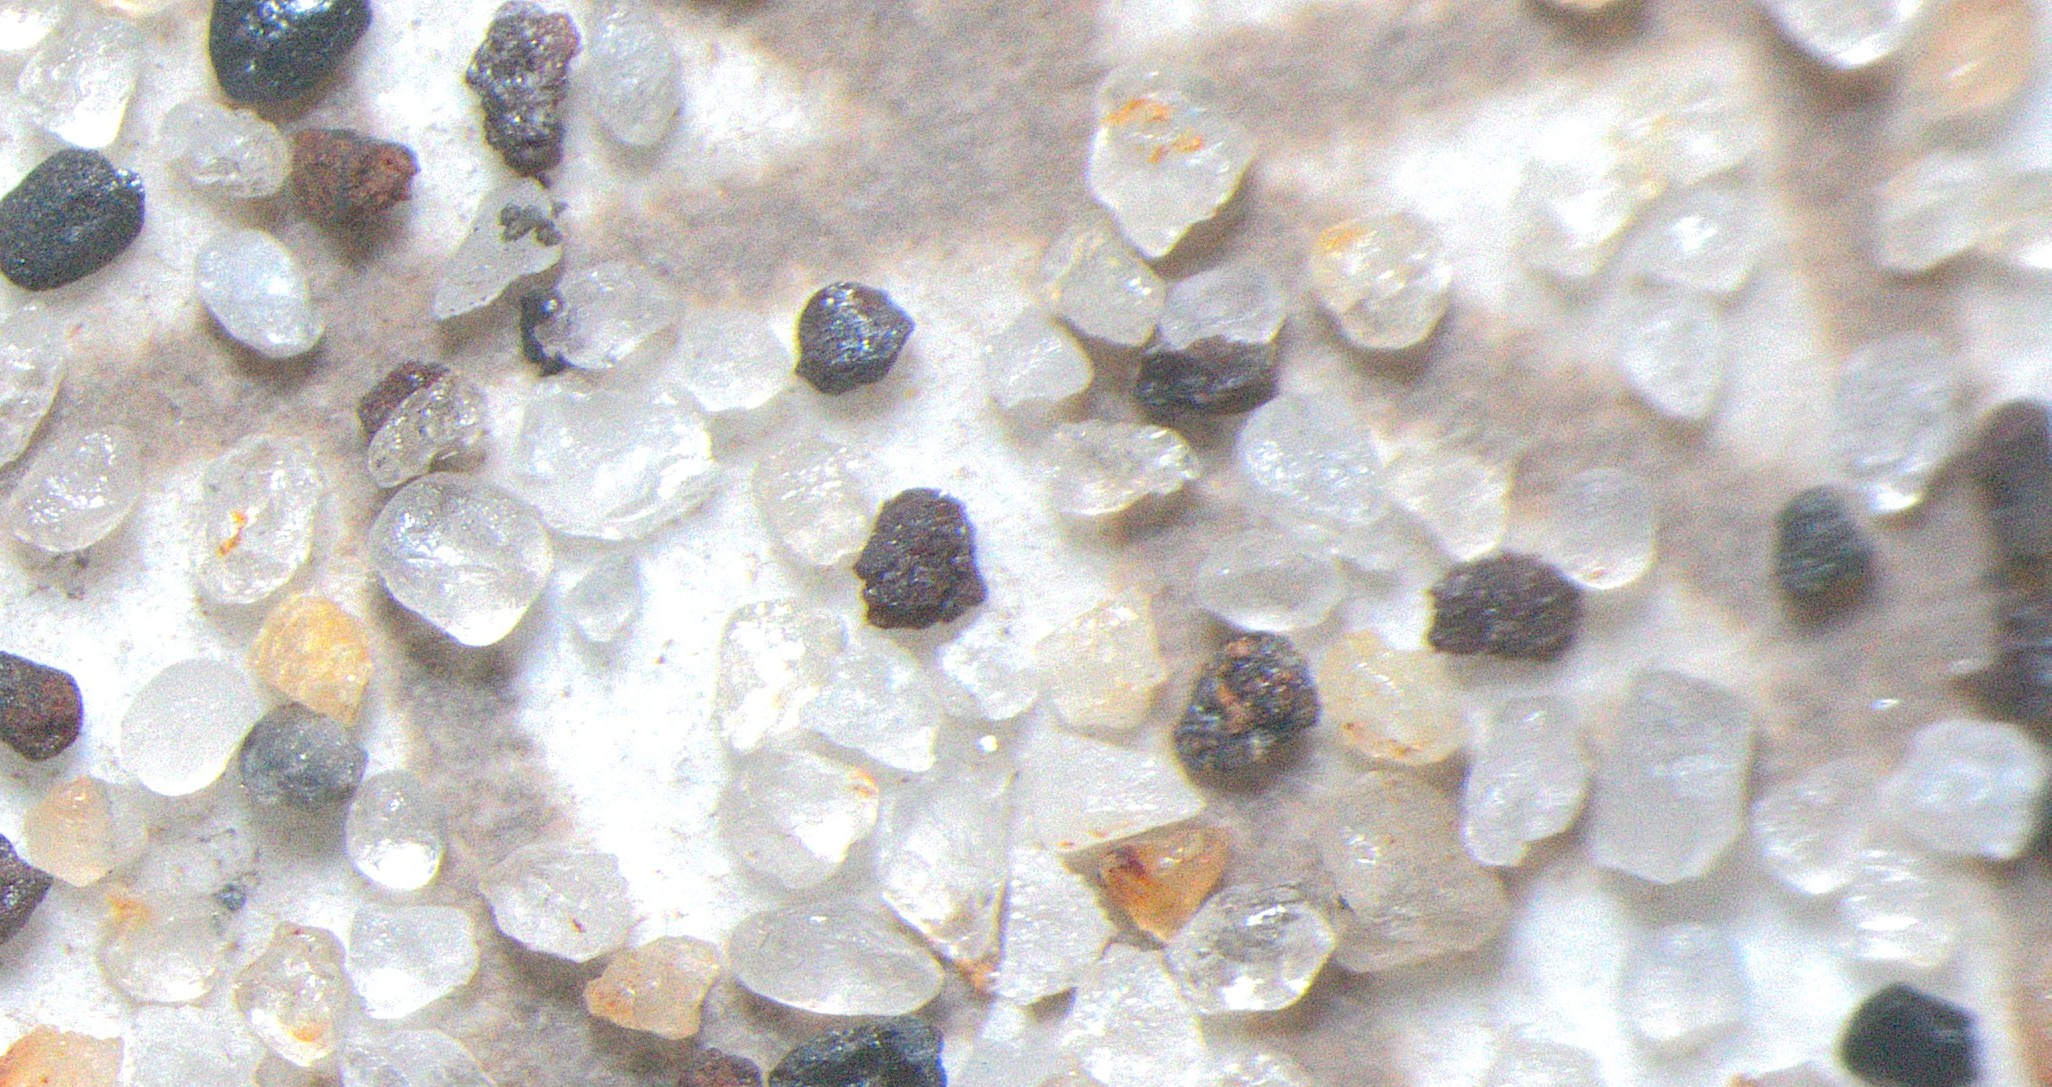
\includegraphics[width=4.05cm,height=4cm,keepaspectratio]{figure/pengujian/5/1347-20_48E_tile1.jpg}}} &
    \multirow{2}{*}{1} &

    10\rule{0pt}{3.0em} & 1 & 0 & 0 & 9 & 0 & 1{,}000 & 0{,}951 & 1 &
    V1 \textit{(Am)} \\

    \cline{4-13}

    & & &   % ← WAJIB: kosongkan No | Citra | GT Total
    11\rule{0pt}{3.0em} & 1 & 0 & 0 & 10 & 0 & 0{,}900 & \textit{NaN} & 1 &
    V2 \textit{(Std)} \\

    \hline

    % ===== Data ke-6 =====
    \multirow{2}{*}{6} &
    \multirow{2}{*}{%
    \parbox[c][1.5cm][c]{4cm}{%
    \centering
    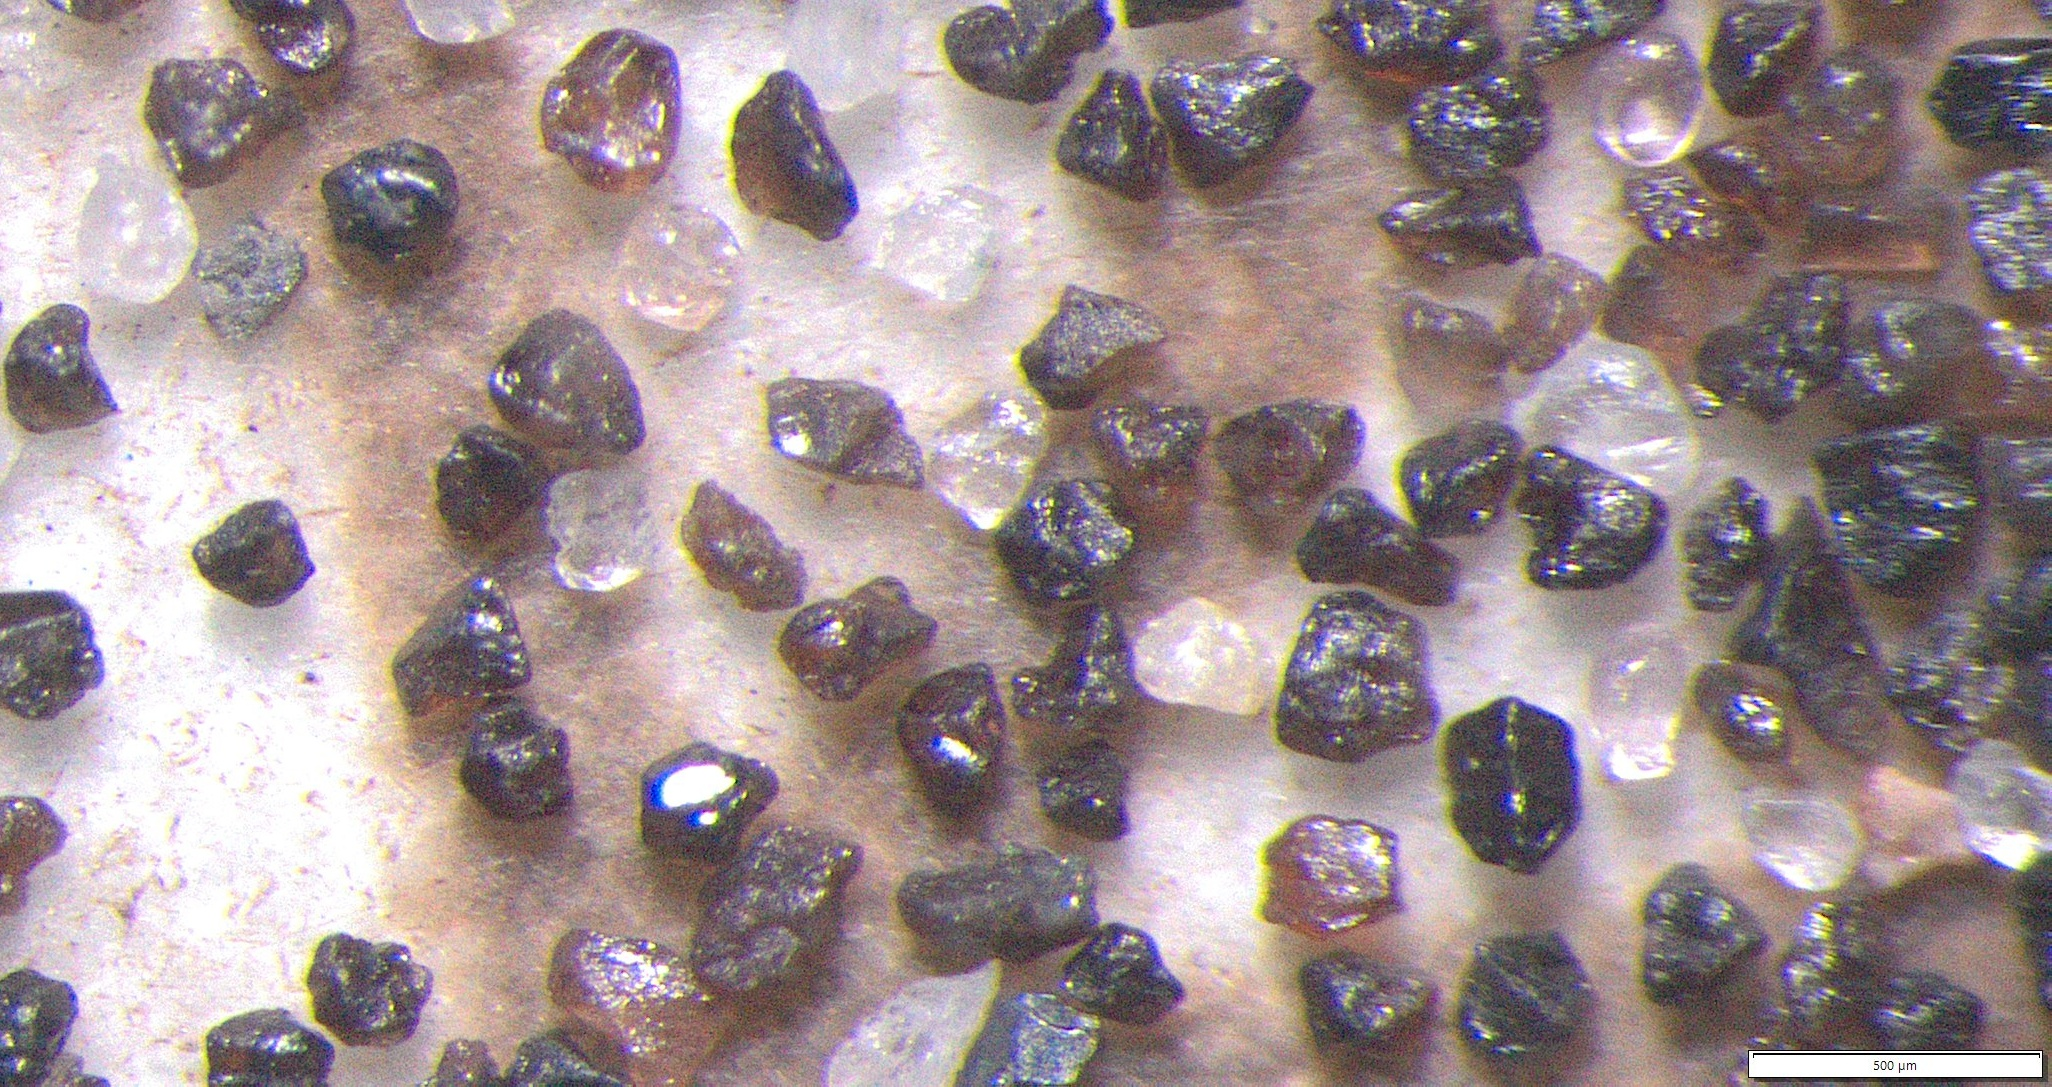
\includegraphics[width=4.05cm,height=4cm,keepaspectratio]{figure/pengujian/6/0384-16_100H_tile3.jpg}}} &
    \multirow{2}{*}{31} &

    46\rule{0pt}{3.0em} & 17 & 7 & 1 & 21 & 6 & 0{,}687 & 0{,}921 & 25 &
    V1 \textit{(Am)} \\

    \cline{4-13}

    & & &   % ← WAJIB: kosongkan No | Citra | GT Total
    71\rule{0pt}{3.0em} & 30 & 0 & 0 & 41 & 1 & 0{,}852 & 0{,}924 & 30 &
    V2 \textit{(Std)} \\

    \hline

\end{longtable}
\end{landscape}
\restoregeometry

Berdasarkan Tabel \ref{table:4.Pengujian1}, hasil pengujian menunjukkan perbedaan karakteristik antara kedua model berdasarkan beberapa kategori evaluasi deteksi. Model V2 \textit{Standard} mampu mengidentifikasi objek kasiterit dengan akurasi yang tinggi, sebagaimana tercermin dari nilai \APrangefiftyy dan \IoUrangefiftyy yang cukup baik. Namun, model ini cenderung melakukan \textit{overprediction}, yang mengakibatkan tingginya angka \textit{False Positive}. Selain itu, pada data uji ke-5, model V2 \textit{Standard} menghasilkan nilai \IoUrangefiftyy berupa \textit{NaN}, yang mengindikasikan kegagalan deteksi pada ambang batas IoU tertentu, khususnya pada IoU tinggi. Sebaliknya, model V1 \textit{Amodal} menunjukkan performa yang lebih baik dalam hal segmentasi, ditandai dengan nilai \IoUrangefiftyy yang lebih tinggi secara konsisten. Model ini juga lebih stabil dalam melakukan prediksi dan tidak mengalami \textit{overprediction} seperti model V2 \textit{Standard}, sehingga menghasilkan jumlah \textit{False Positive} yang lebih rendah. Namun, stabilitas tersebut berdampak pada nilai \APrangefiftyy yang cenderung lebih rendah dibandingkan model V2 \textit{Standard}, mengindikasikan bahwa model V1 \textit{Amodal} lebih konservatif dalam melakukan prediksi. \par

\begin{figure}[H]
    \centering
    % Baris pertama: dua gambar sejajar
    \begin{subfigure}[b]{0.475\textwidth}
        \centering
        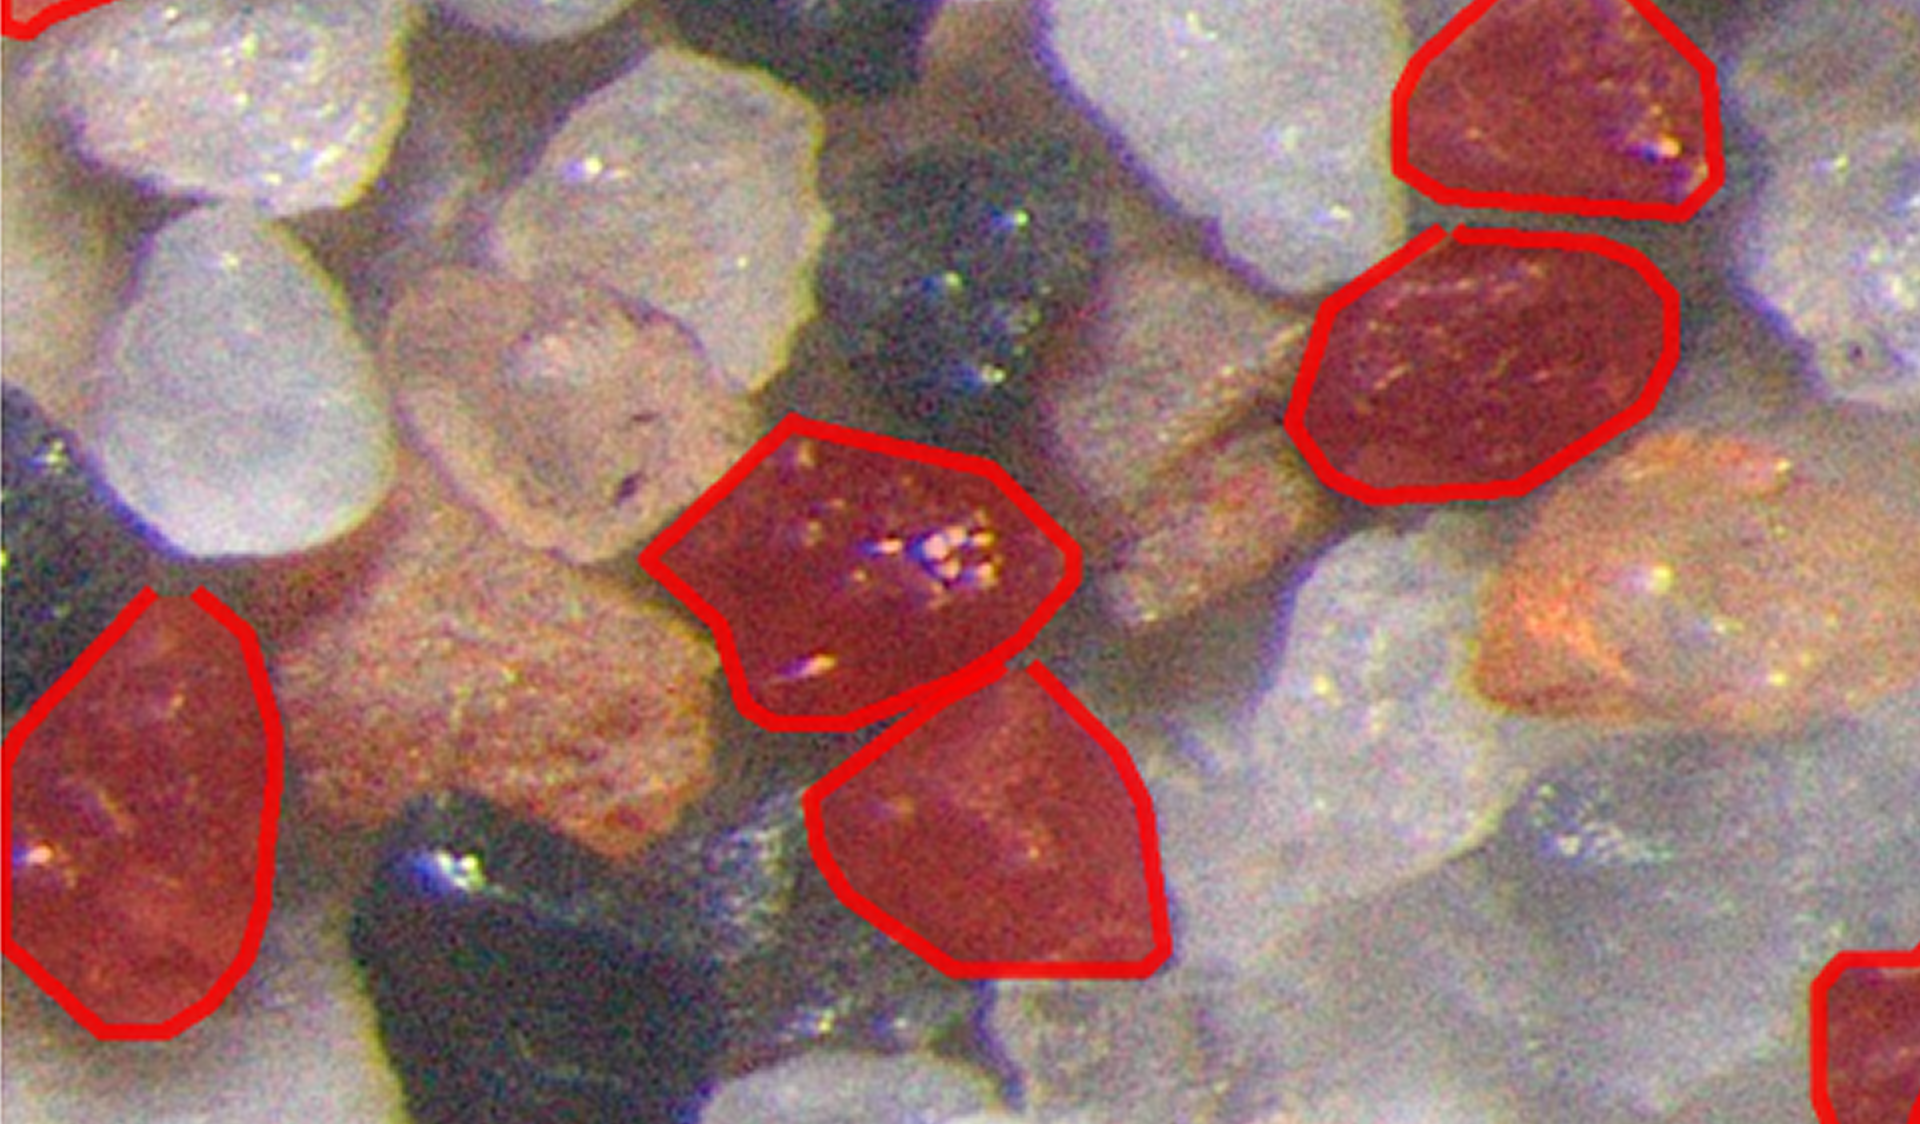
\includegraphics[width=\textwidth]{figure/oklusi/tile_2 - GT.png}
        \caption{Citra Ground Truth}
        \label{fig:4.Citra_gt}
    \end{subfigure}
    
    % Baris kedua: satu gambar di bawah tengah
    \vskip\baselineskip
    \begin{subfigure}[b]{0.475\textwidth}
        \centering
        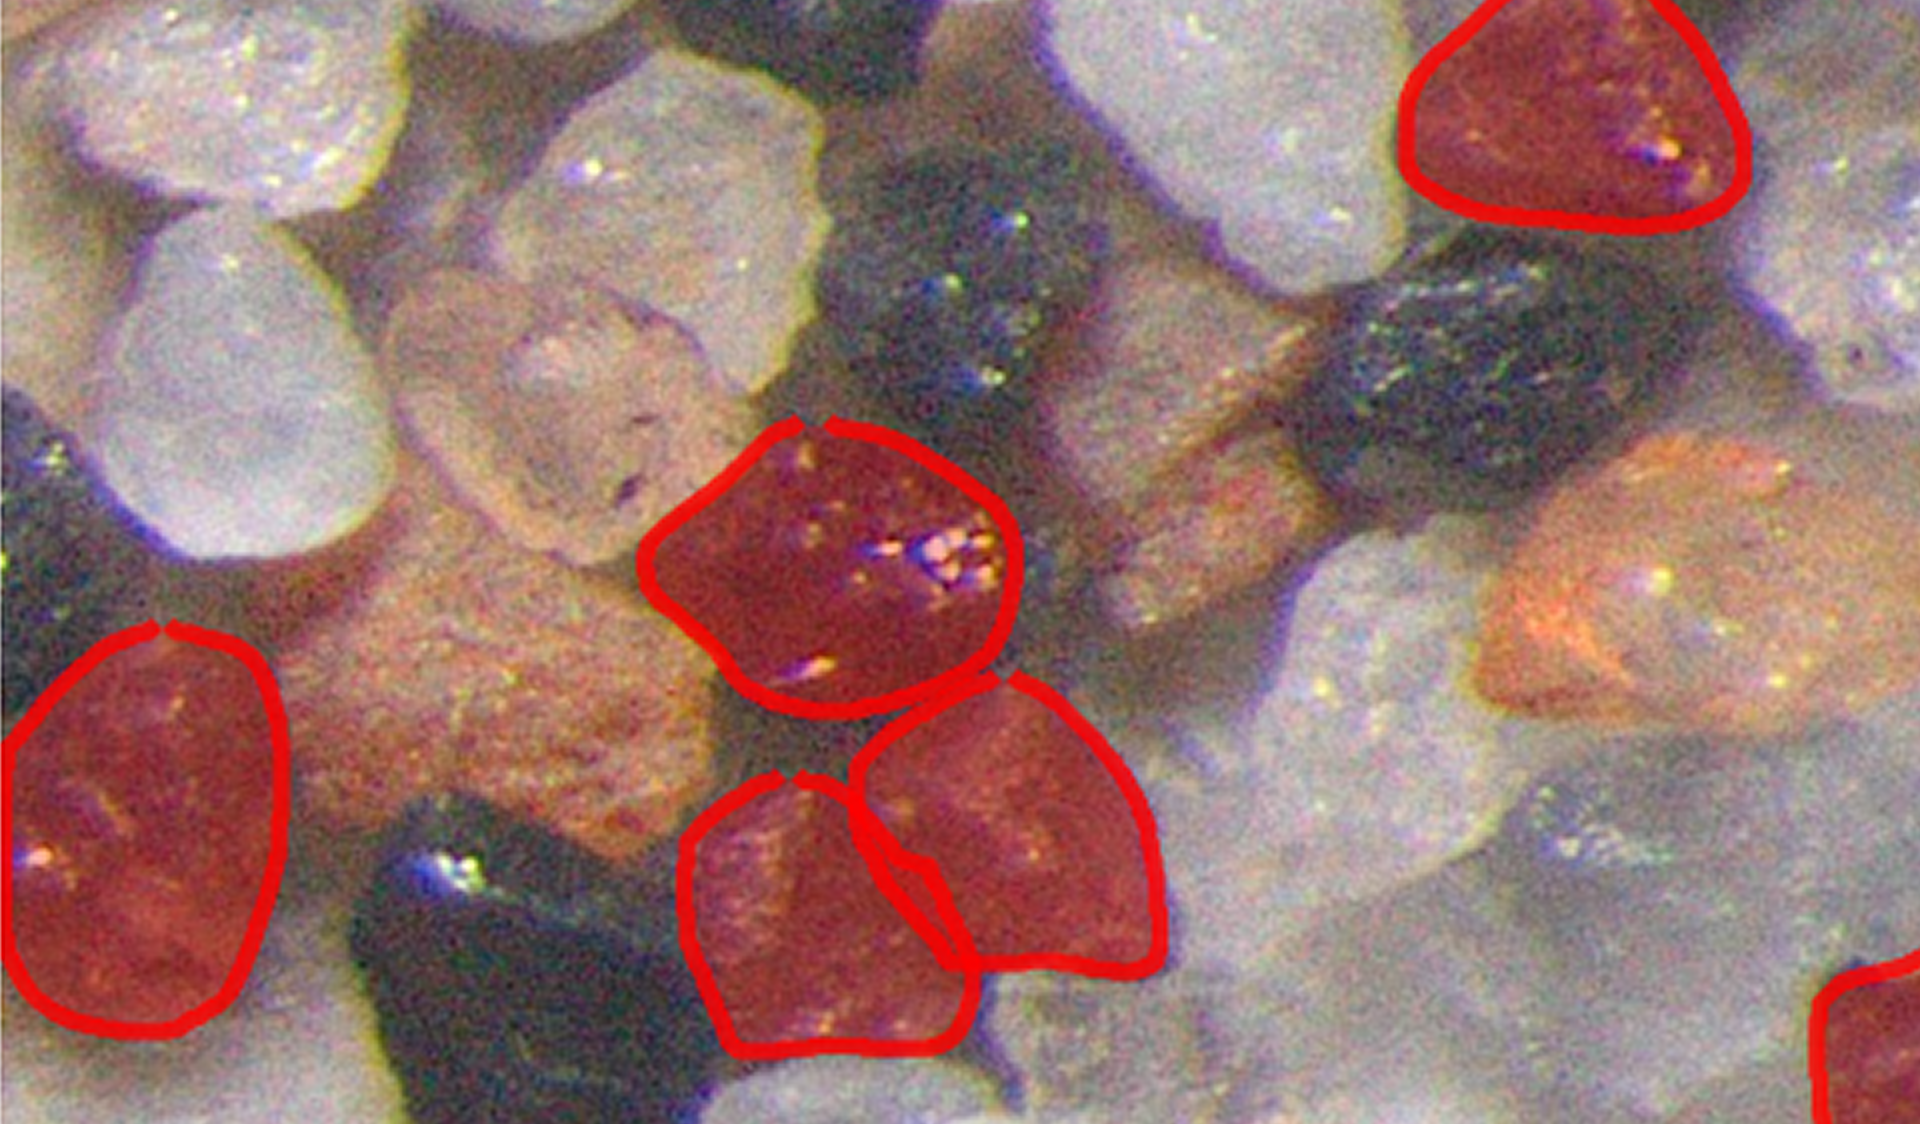
\includegraphics[width=\textwidth]{figure/oklusi/tile_2 - Amodal.png}
        \caption{Hasil Prediksi Model V1 \textit{Amodal} \textit{Adam}}
        \label{fig:4.hasil_amodal}
    \end{subfigure}
    \hfill
    \begin{subfigure}[b]{0.475\textwidth}
        \centering
        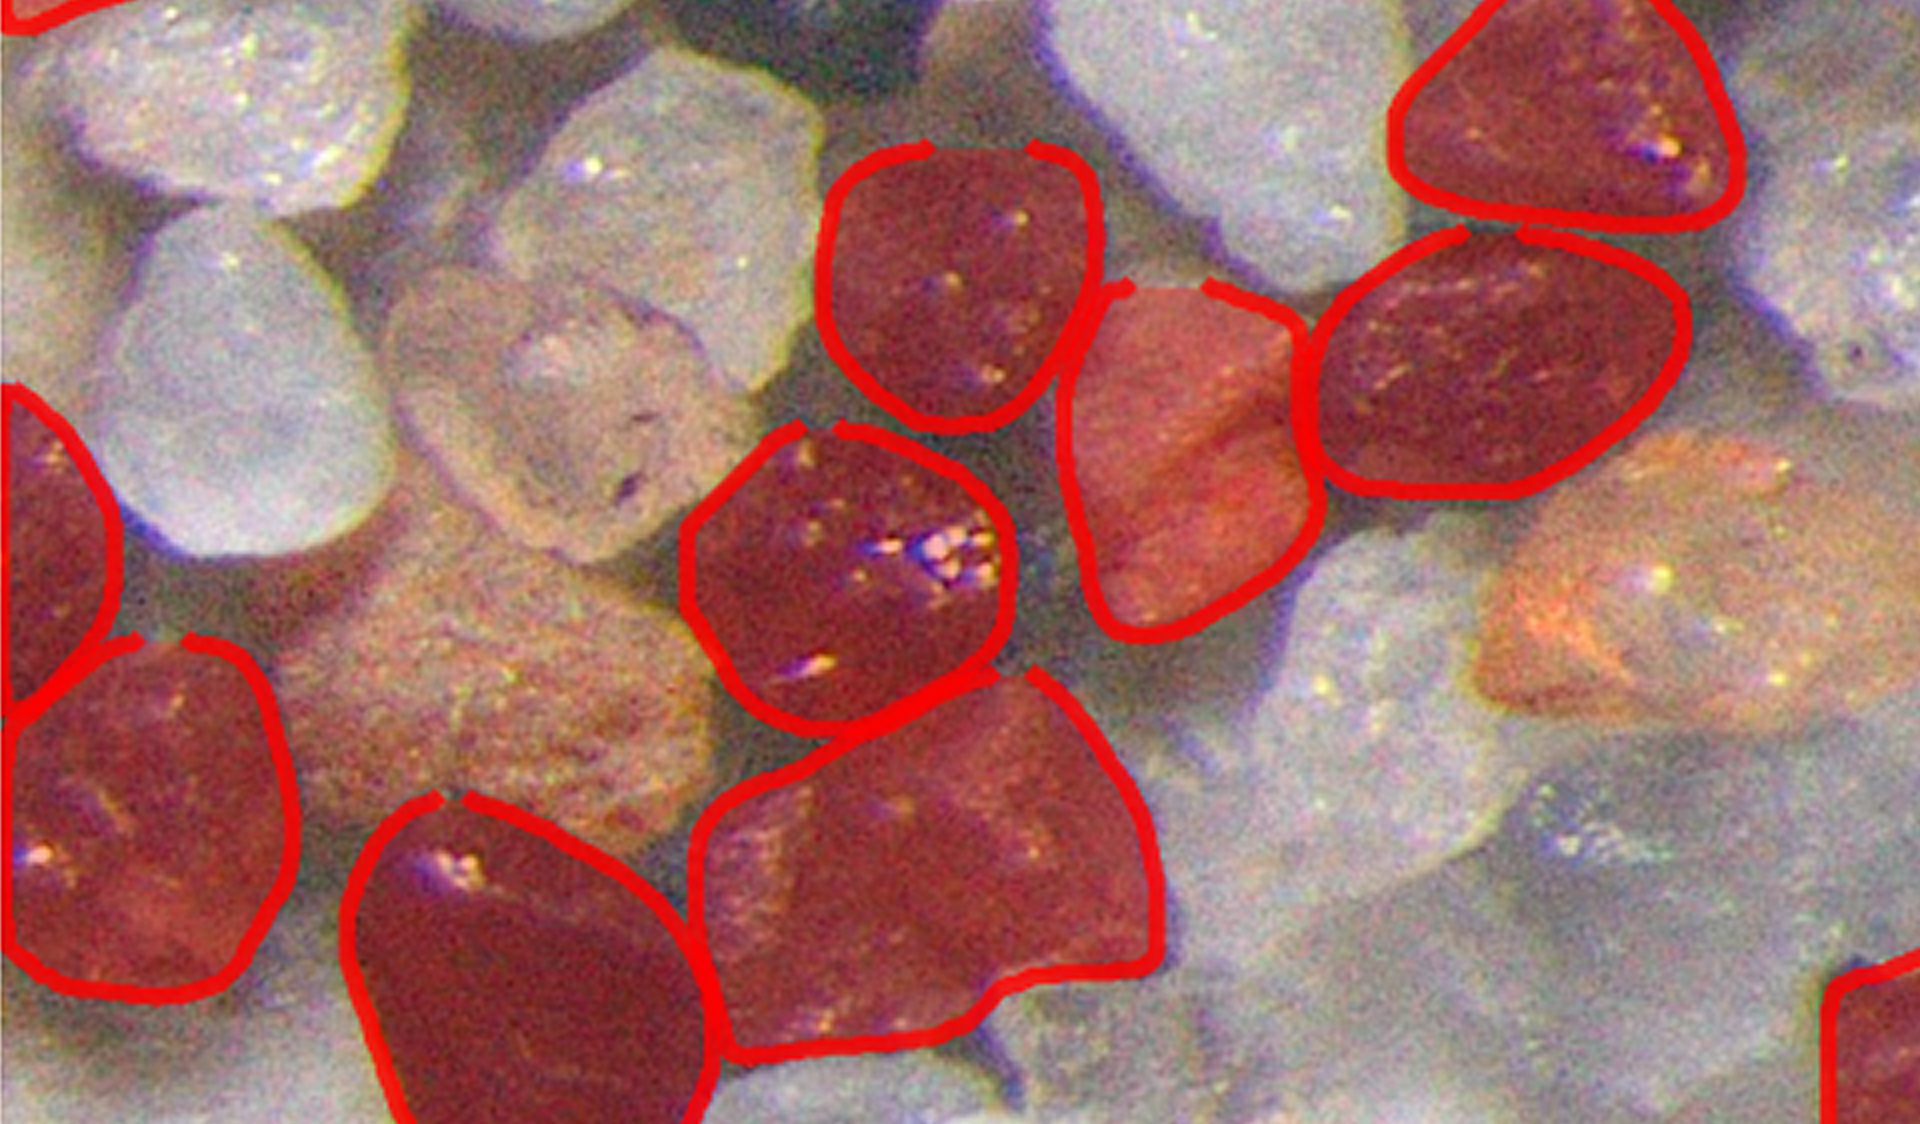
\includegraphics[width=\textwidth]{figure/oklusi/tile_2 - Standard.png}
        % \caption{Hasil \textit{Flip} Vertical ($\shortdownarrow$)}
        \caption{Hasil Prediksi Model V2 \textit{Standard} SGD}
        % \caption{Hasil \textit{Flip} Vertical ($\downarrow$)}

        \label{fig:4.hasil_stadard}
    \end{subfigure}
    \caption{Contoh Hasil Oklusi dengan Objek}
    \label{fig:4.Hasil_oklusi_dengan_objek}
\end{figure}

Berdasarkan pada Gambar \ref{fig:4.Hasil_oklusi_dengan_objek}, terlihat bahwa pada area kasiterit yang saling bersebelahan dan mengalami oklusi, model V1 \textit{Amodal} dengan \textit{optimizer Adam} mampu memisahkan dan memprediksi masing-masing butir kasiterit secara individual, meskipun sebagian bentuk objek tertutup oleh butir lain. Hal ini tampak dari beberapa area berwarna merah yang tetap tersegmentasi sebagai objek terpisah sesuai dengan anotasi \textit{Ground Truth}. Sebaliknya, pada hasil model V2 \textit{Standard} dengan \textit{optimizer} SGD, area kasiterit yang saling menutupi tersebut cenderung diprediksi sebagai satu objek utuh, sehingga batas antar butir yang berdekatan tidak terpisahkan dengan baik. Perbedaan ini menunjukkan bahwa pendekatan \textit{amodal} lebih efektif dalam menangani kondisi oklusi antar butir kasiterit dibandingkan pendekatan \textit{standard} yang bergantung pada area objek yang tampak secara visual.

\begin{figure}[H]
    \centering
    % Baris pertama: dua gambar sejajar
    \begin{subfigure}[b]{0.475\textwidth}
        \centering
        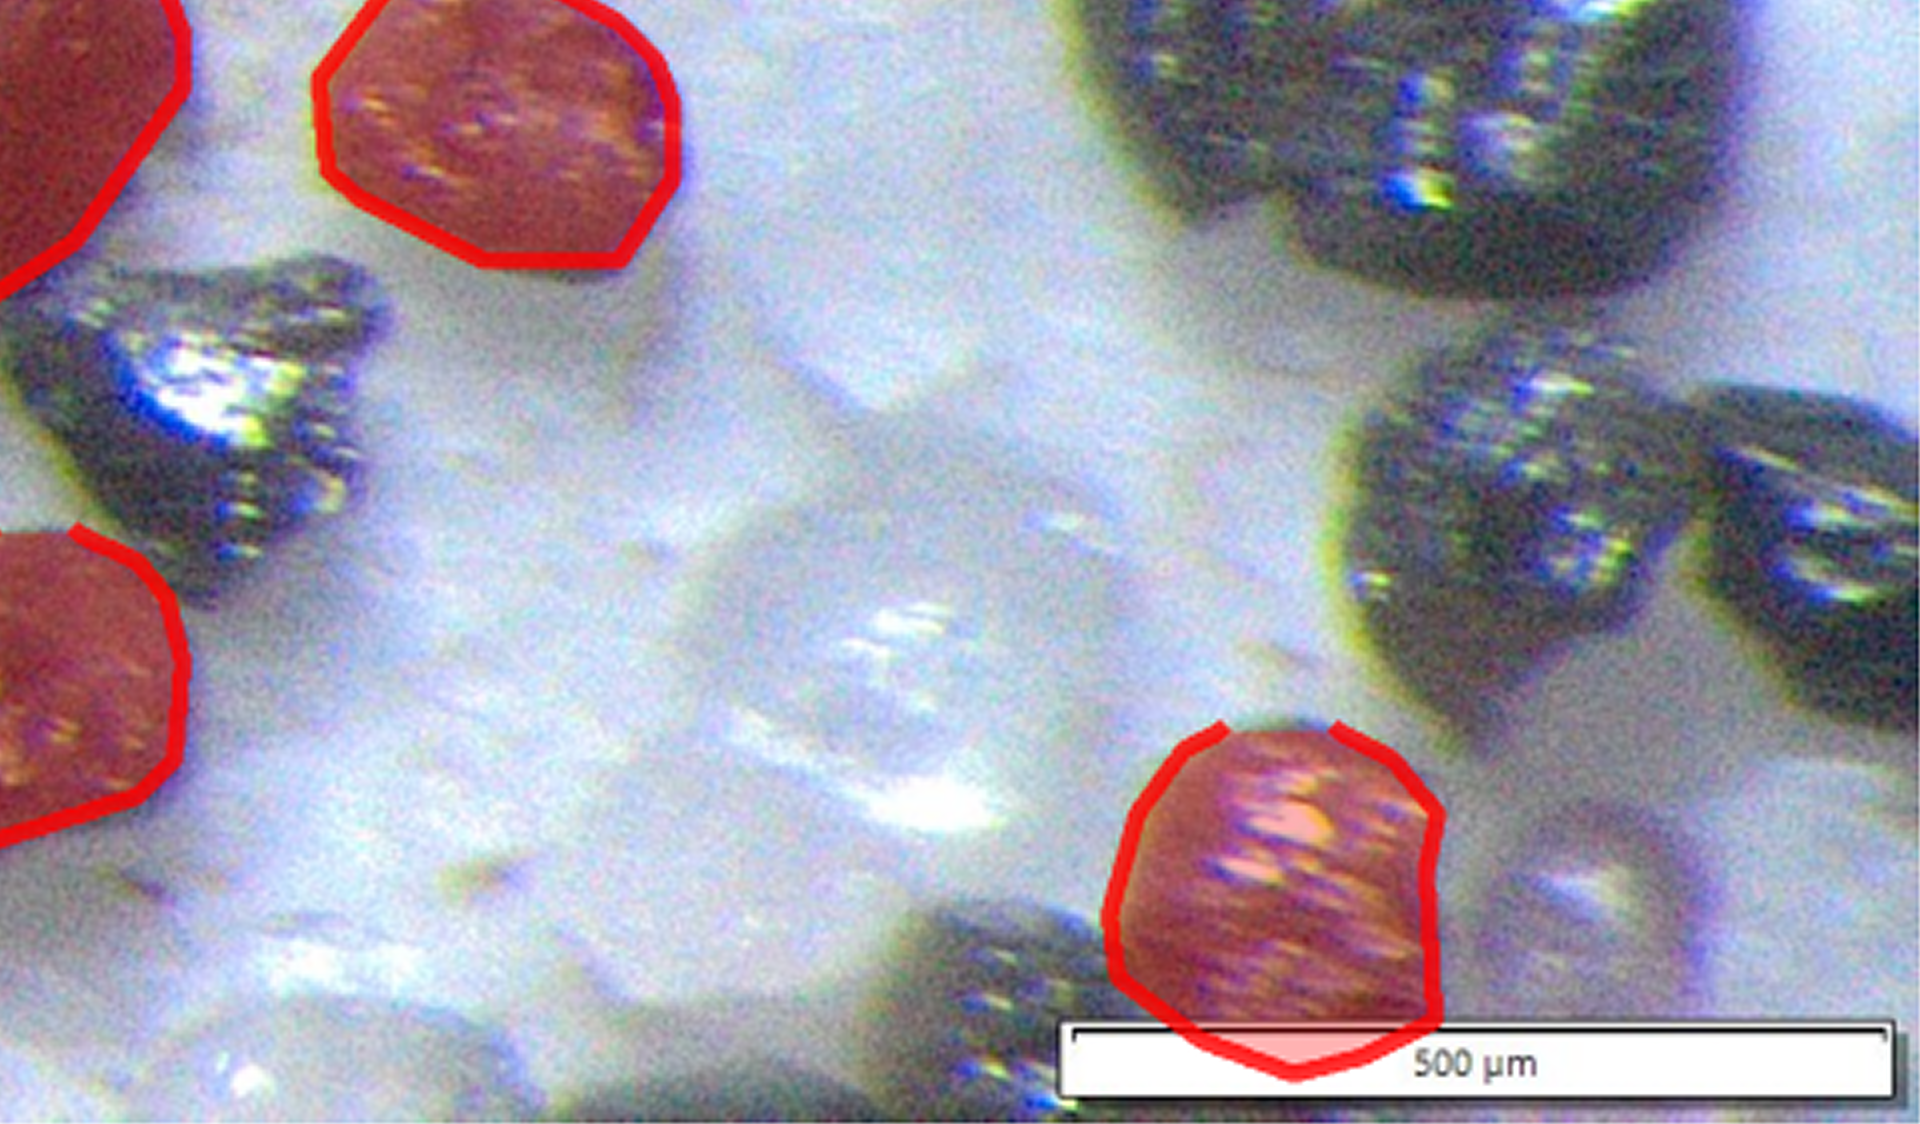
\includegraphics[width=\textwidth]{figure/oklusi/tile_4 - GT.png}
        \caption{Citra Ground Truth}
        \label{fig:4.Citra_gt1}
    \end{subfigure}
    
    % Baris kedua: satu gambar di bawah tengah
    \vskip\baselineskip
    \begin{subfigure}[b]{0.475\textwidth}
        \centering
        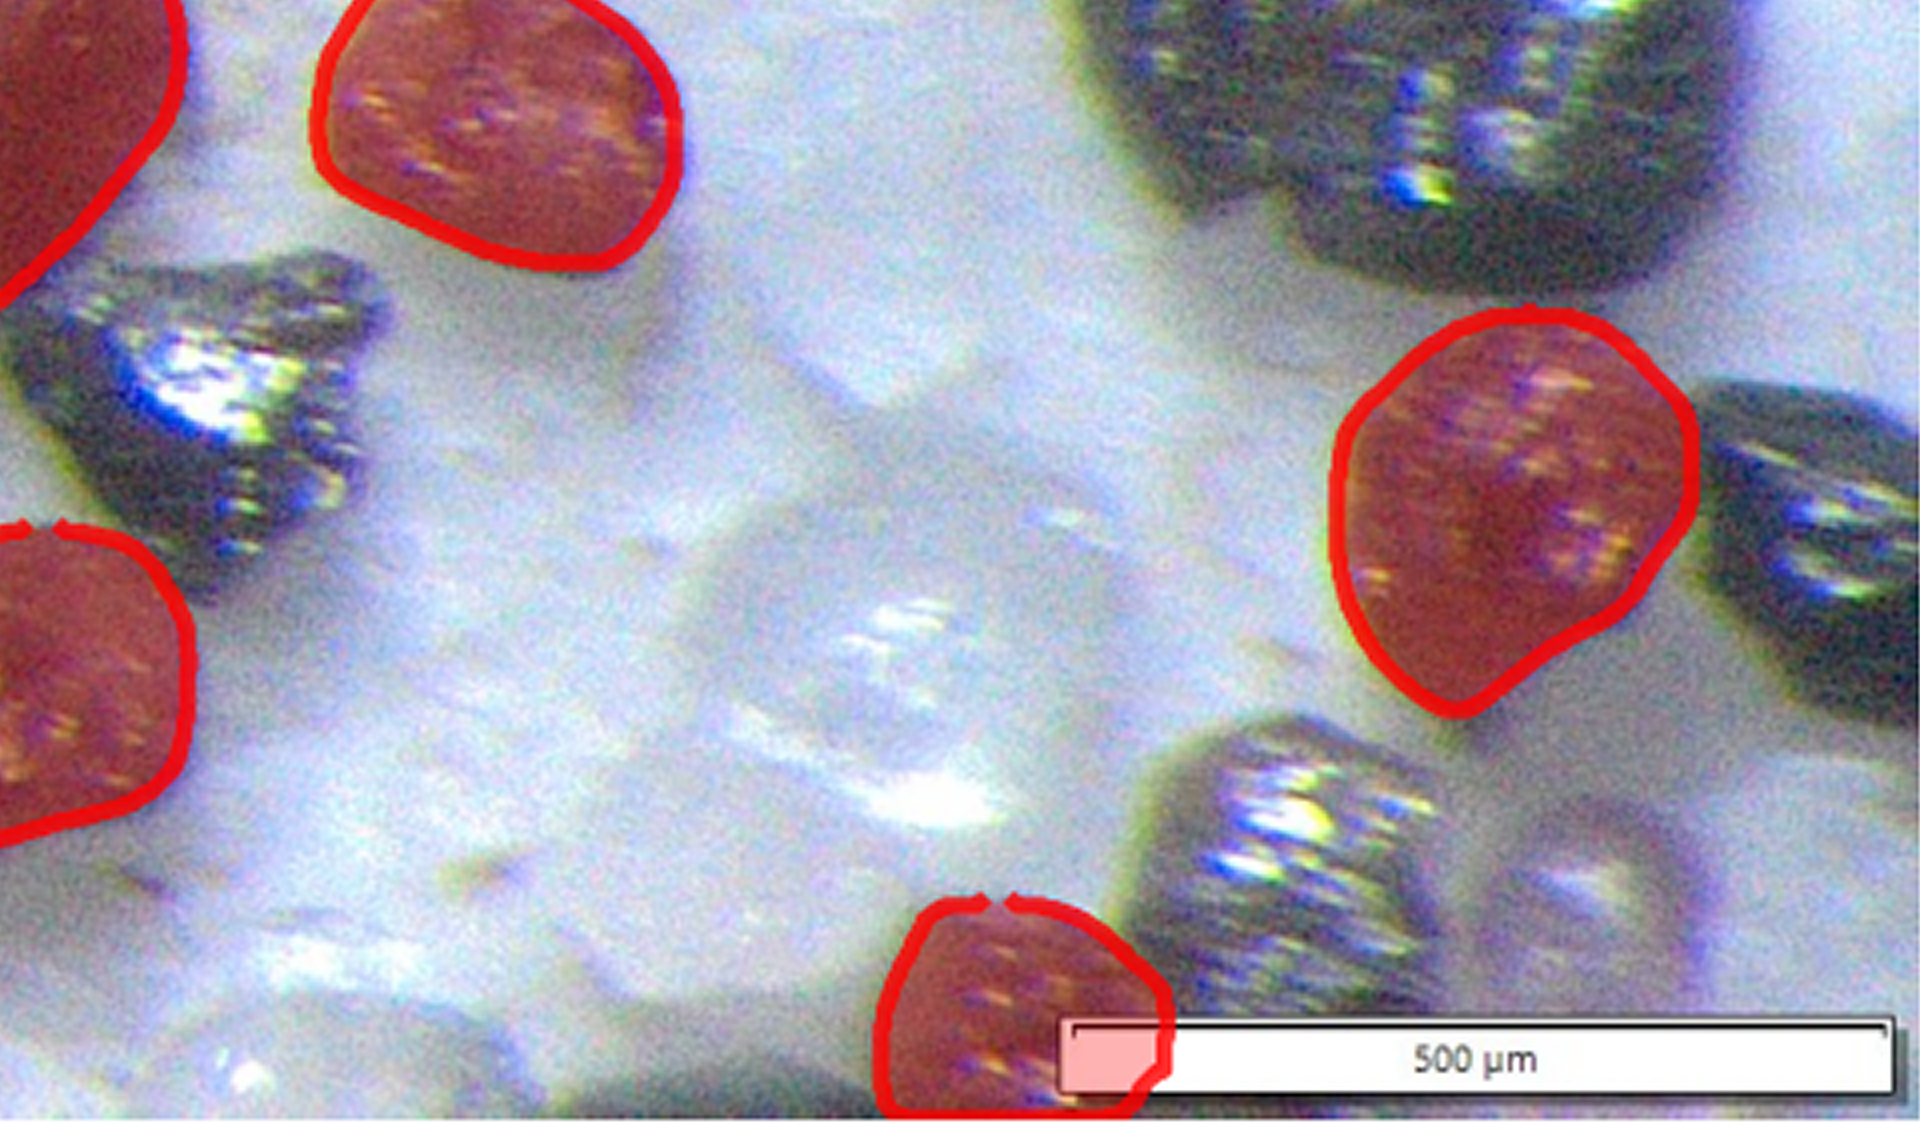
\includegraphics[width=\textwidth]{figure/oklusi/tile_4 - Amodal.png}
        \caption{Hasil Prediksi Model V1 \textit{Amodal} \textit{Adam}}
        \label{fig:4.hasil_amodal1}
    \end{subfigure}
    \hfill
    \begin{subfigure}[b]{0.475\textwidth}
        \centering
        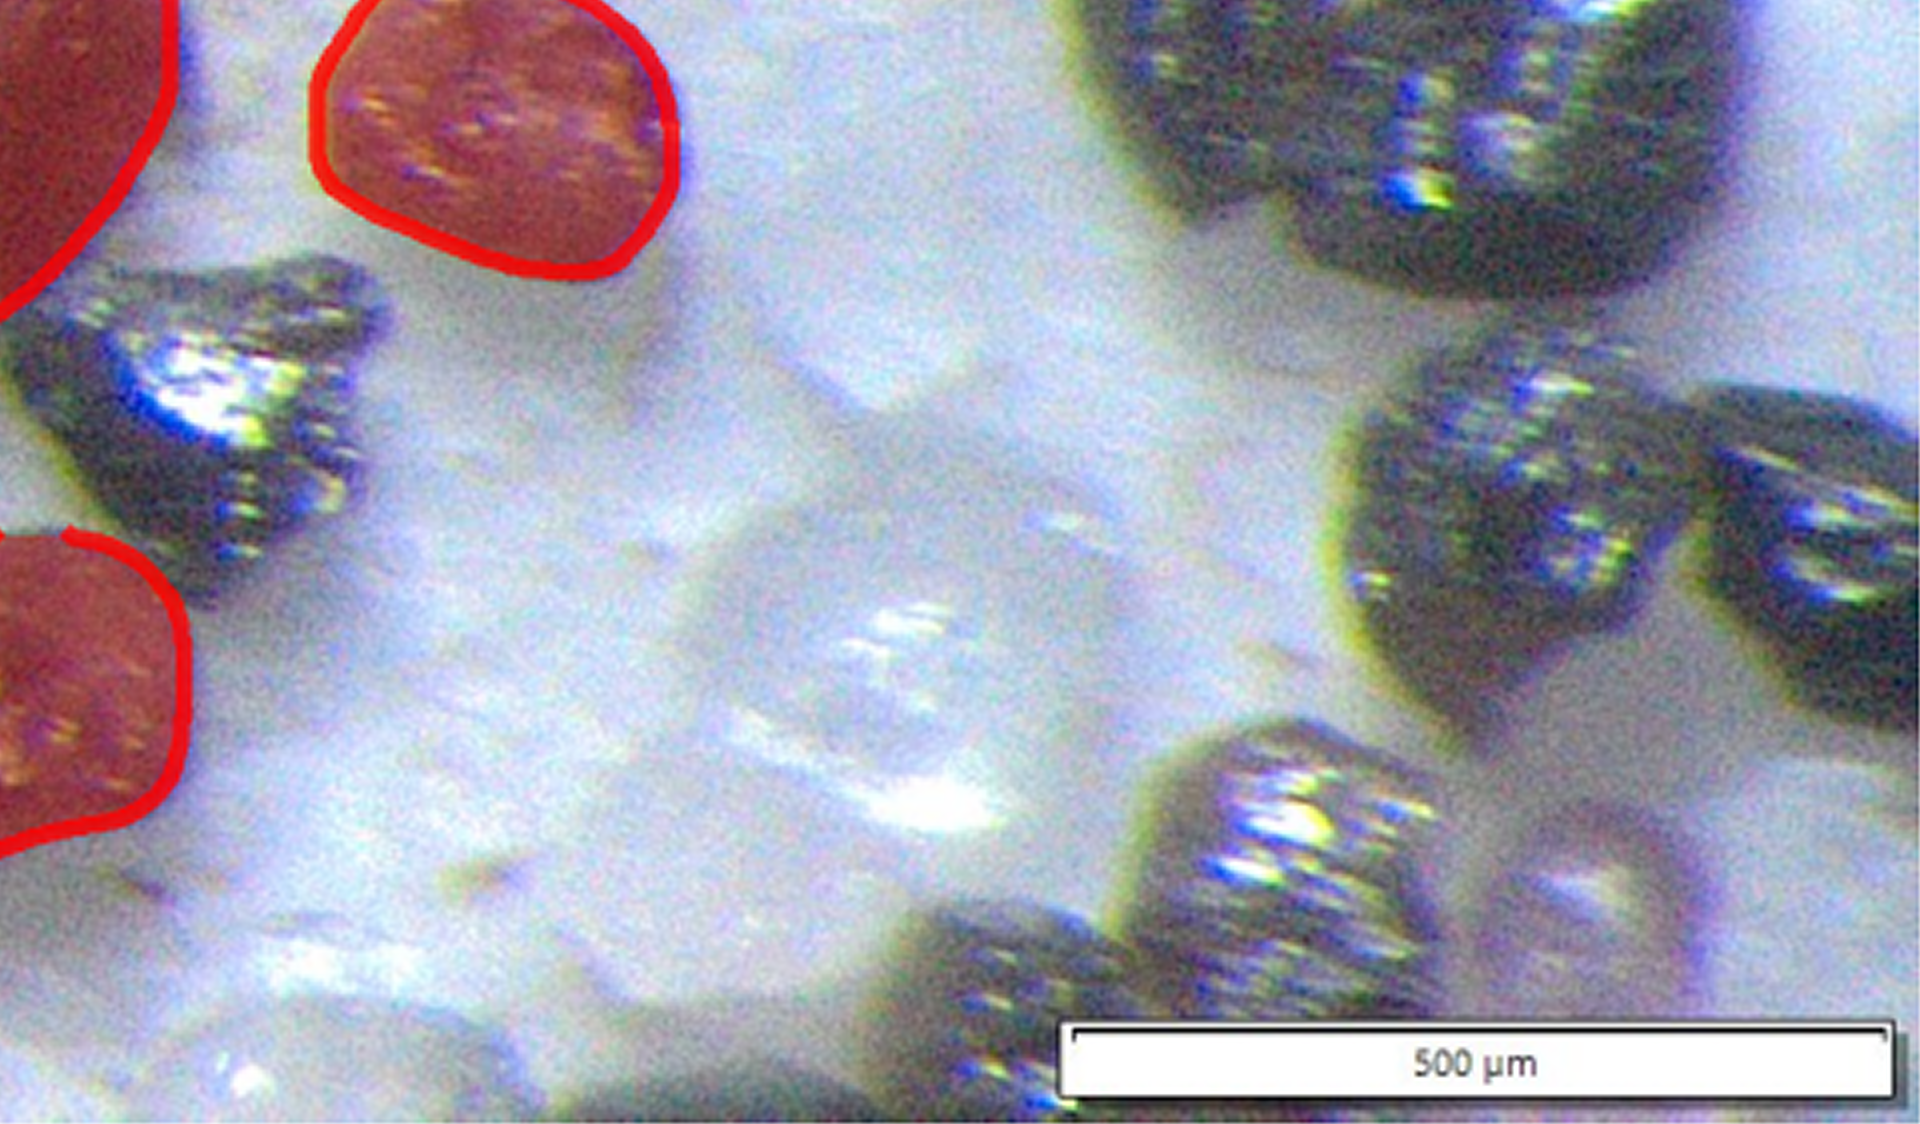
\includegraphics[width=\textwidth]{figure/oklusi/tile_4 - Standard.png}
        % \caption{Hasil \textit{Flip} Vertical ($\shortdownarrow$)}
        \caption{Hasil Prediksi Model V2 \textit{Standard} SGD}
        % \caption{Hasil \textit{Flip} Vertical ($\downarrow$)}

        \label{fig:4.hasil_stadard1}
    \end{subfigure}
    \caption{Contoh Hasil Oklusi dengan Background}
    \label{fig:4.Hasil_oklusi_dengan_bg}
\end{figure}

Berdasarkan pengamatan pada Gambar \ref{fig:4.Hasil_oklusi_dengan_bg}, terlihat bahwa pada bagian pojok kanan citra terdapat elemen latar belakang berupa penanda skala (500 $\mu$m) yang menutupi sebagian objek kasiterit. Pada kondisi ini, berdasarkan perbandingan dengan \textit{ground truth} yang berjumlah empat objek kasiterit, model V1 \textit{amodal} dengan \textit{optimizer} \textit{Adam} menghasilkan lima prediksi, dengan tiga objek terdeteksi dengan benar, satu objek tidak terdeteksi, serta dua prediksi yang termasuk kesalahan deteksi. Meskipun terdapat kesalahan, model V1 tetap mampu melakukan segmentasi pada salah satu objek kasiterit yang teroklusi oleh latar belakang, di mana area objek masih diprediksi meskipun sebagian tertutup elemen non-objek. Sebaliknya, model V2 \textit{standard} dengan \textit{optimizer} SGD hanya menghasilkan tiga deteksi yang benar dan satu objek tidak terdeteksi, serta tidak mampu melakukan segmentasi pada area yang mengalami oklusi sehingga tidak menghasilkan prediksi pada lokasi tersebut. Hal ini menunjukkan bahwa model \textit{amodal} memiliki kemampuan yang lebih baik dalam mengenali keberadaan kasiterit pada kondisi oklusi oleh latar belakang dibandingkan model \textit{standard} yang sangat bergantung pada visibilitas penuh objek. \par

\section{Analisis Hasil Keseluruhan} \label{IV.Analisis_Hasil_Keseluruhan}
Dalam penelitian ini, metrik \textit{Average Precision} pada rentang \textit{Intersection over Union} 0{,}50 hingga 0{,}95 (\APrangefifty) digunakan sebagai indikator utama dalam menentukan konfigurasi model terbaik karena mampu merepresentasikan kinerja model secara konsisten pada berbagai tingkat ambang \textit{IoU}. Metrik ini memberikan gambaran objektif mengenai akurasi deteksi dan presisi segmentasi model pada kondisi evaluasi yang bervariasi. Selain itu, metrik \IoUrangefiftyy digunakan untuk menilai tingkat kesesuaian segmentasi antara hasil prediksi dan \textit{ground truth}. Kombinasi kedua metrik tersebut memungkinkan evaluasi performa model yang lebih komprehensif dan terukur. \par

Pada hasil percobaan dari variasi konfigurasi pelatihan model terbaik pada \textit{Mask} R-CNN ResNet50 FPN V1 dan V2, didapatkan bahwa model \textit{pre-trained} \textit{Mask} R-CNN ResNet50 FPN V1 dengan variasi model \textit{Amodal} dan \textit{optimizer} \textit{Adam} menunjukkan performa terbaik dengan nilai \textit{AP50:95} sebesar 0{,}458 dan \textit{IoU50:95} sebesar 0{,}915. Model \textit{pre-trained} \textit{Mask} R-CNN ResNet50 FPN V2 dengan variasi model \textit{Standard} dan \textit{optimizer} SGD menunjukkan performa yang sedikit lebih rendah dengan nilai \textit{AP50:95} sebesar 0{,}449 dan \textit{IoU50:95} sebesar 0{,}915. Nilai tersebut memiliki selisih nilai \textit{AP50:95} sebesar 0{,}009 (0{,}9\%) dan nilai \textit{IoU50:95} sama, yang menunjukkan variasi model V1 \textit{Amodal} lebih unggul dibandingkan variasi model V2 \textit{Standard}.  \par

Penerapan teknik \textit{Amodal Instance Segmentation} menunjukkan pengaruh yang berbeda-beda pada kinerja model \textit{Mask} R-CNN. Pada model \textit{pre-trained} Mask R-CNN ResNet50 FPN V1 dengan \textit{optimizer} Adam, penambahan pendekatan \textit{amodal} yang meningkatkan jumlah parameter sebesar 2.950.914 (6{,}75\%) mampu meningkatkan performa, ditunjukkan oleh kenaikan nilai \textit{AP50:95} dari 0{,}437 menjadi 0{,}458 serta peningkatan \textit{IoU50:95} dari 0{,}910 menjadi 0{,}915, dengan tambahan waktu pelatihan sebesar 0{,}37 jam. Sebaliknya, pada model \textit{pre-trained} Mask R-CNN ResNet50 FPN V2 dengan \textit{optimizer} SGD, penerapan teknik \textit{amodal} yang menambah parameter sebesar 2.950.914 (6{,}46\%) justru menurunkan performa, dengan nilai \textit{AP50:95} berkurang dari 0{,}449 menjadi 0{,}420 dan \textit{IoU50:95} dari 0{,}915 menjadi 0{,}913, meskipun waktu pelatihan hanya bertambah 0{,}45 jam. Hasil ini menunjukkan bahwa peningkatan kompleksitas melalui pendekatan \textit{amodal} tidak selalu berbanding lurus dengan peningkatan kinerja, serta sangat bergantung pada arsitektur \textit{pre-trained} dan pemilihan \textit{optimizer}. \par

Dari segi efisiensi parameter, peningkatan kompleksitas model tidak selalu berbanding lurus dengan peningkatan efisiensi parameter. Model \textit{Mask} R-CNN ResNet50 FPN V1 \textit{Standard} dengan \textit{optimizer} SGD menunjukkan efisiensi parameter tertinggi dengan total 43{,}699{,}995 parameter serta rasio \textit{AP/Param} sebesar $9{,}999\times10^{-9}$ dan \textit{IoU/Param} sebesar $2{,}082\times10^{-8}$. Penerapan pendekatan \textit{amodal} pada V1 meningkatkan jumlah parameter menjadi 46{,}650{,}909, namun justru menurunkan efisiensi rasio kinerja terhadap parameter. Pola serupa juga terlihat pada varian V2, di mana model \textit{Standard} dengan \textit{optimizer} SGD (\textit{Param Ratio} 1{,}045$\times$) menunjukkan keseimbangan yang lebih baik dibandingkan model V2 \textit{Amodal} (\textit{Param Ratio} 1{,}113$\times$). Dengan demikian, meskipun pendekatan \textit{amodal} unggul dalam menangani oklusi, model \textit{Standard} khususnya pada varian V2 lebih sesuai untuk penerapan praktis segmentasi mineral kasiterit dari sisi efisiensi dan stabilitas kinerja. \par

Hasil pengujian menunjukkan adanya perbedaan karakteristik yang jelas antara kedua model. Model V2 \textit{standard} mampu mengidentifikasi objek kasiterit dengan akurasi yang tinggi, sebagaimana ditunjukkan oleh nilai \APrangefiftyy dan \IoUrangefiftyy yang relatif baik, namun cenderung mengalami \textit{overprediction} sehingga menghasilkan jumlah \textit{False Positive} yang lebih tinggi. Kondisi ini semakin terlihat pada data uji ke-5, di mana model V2 \textit{standard} menghasilkan nilai \IoUrangefiftyy berupa NaN, yang mengindikasikan kegagalan deteksi pada ambang batas IoU tertentu, khususnya pada IoU tinggi. Sebaliknya, model V1 \textit{amodal} menunjukkan performa segmentasi yang lebih stabil dan konsisten dengan nilai \IoUrangefiftyy yang lebih tinggi, serta tidak mengalami \textit{overprediction}, sehingga jumlah \textit{False Positive} yang dihasilkan lebih rendah. Namun, stabilitas dan sifat prediksi yang lebih konservatif tersebut berdampak pada nilai \APrangefiftyy yang cenderung lebih rendah dibandingkan model V2 \textit{standard}. \par

Hasil pengamatan pada contoh oklusi antar kasiterit dan oklusi dengan latar belakang, dapat dilihat bahwa model V1 \textit{Amodal} dengan \textit{optimizer} \textit{Adam} menunjukkan kemampuan yang lebih baik dalam mendeteksi objek kasiterit pada kondisi oklusi. Pada kasus kasiterit yang saling bersebelahan, model amodal mampu memisahkan dan memprediksi masing-masing butir kasiterit secara individual meskipun sebagian objek tertutup, sehingga hasil segmentasi tetap sesuai dengan anotasi \textit{Ground Truth}. Selain itu, pada kondisi oklusi oleh elemen latar belakang berupa penanda skala, model amodal masih mampu mendeteksi keberadaan kasiterit yang tertutup sebagian oleh \textit{background}. Sebaliknya, model V2 \textit{Standard} dengan \textit{optimizer} SGD cenderung memprediksi area kasiterit yang saling menutupi sebagai satu objek utuh serta gagal mendeteksi kasiterit yang teroklusi oleh latar belakang. Hasil ini menunjukkan bahwa pendekatan \textit{amodal} lebih efektif dalam menangani berbagai jenis oklusi, baik antar objek maupun dengan latar belakang. \par

Secara keseluruhan, hasil komparasi menunjukkan bahwa model \textit{pre-trained} \textit{Mask} R-CNN ResNet50 FPN V1 dengan pendekatan \textit{Amodal} dan \textit{optimizer} \textit{Adam} memberikan performa segmentasi yang lebih stabil dan unggul dalam menangani kondisi oklusi, ditunjukkan oleh nilai \textit{AP50:95} yang sedikit lebih tinggi, \textit{IoU50:95} yang konsisten, serta kemampuan mendeteksi objek kasiterit yang tertutup sebagian baik oleh objek lain maupun latar belakang. Sebaliknya, model \textit{Mask} R-CNN ResNet50 FPN V2 \textit{Standard} dengan \textit{optimizer} SGD memiliki efisiensi parameter yang lebih baik dan akurasi deteksi yang kompetitif, namun cenderung menghasilkan \textit{overprediction} dan menunjukkan keterbatasan dalam melakukan segmentasi pada objek yang mengalami oklusi. Dengan demikian, model V1 \textit{Amodal} lebih sesuai untuk skenario analisis citra mikroskop yang kompleks dan beroklusi, sedangkan model V2 \textit{Standard} lebih optimal dari sisi efisiensi dan stabilitas komputasi untuk penerapan praktis dengan kebutuhan sumber daya yang lebih terbatas. \par

% , dibandingkan pendekatan \textit{standard} yang lebih bergantung pada visibilitas visual objek. \par

    \newpage
\chapter{KESIMPULAN DAN SARAN} \label{Bab V}

\section{Kesimpulan} \label{V.Kesimpulan}
Berdasarkan hasil penelitian yang telah dilakukan, dapat diambil beberapa kesimpulan sebagai berikut.

\begin{enumerate}[noitemsep]
    \item Penelitian ini berhasil merancang dan mengembangkan model identifikasi berbasis \textit{Mask} R-CNN yang dapat melakukan segmentasi mineral kasiterit pada citra mikroskop dan mengatasi oklusi antar butir melalui teknik \textit{amodal instance segmentation}. Berdasarkan hasil evaluasi kuantitatif, model \textit{pre-trained Mask} R-CNN ResNet50 FPN V1 dengan pendekatan \textit{amodal} dan \textit{optimizer Adam} menunjukkan performa terbaik dengan nilai \APrangefiftyy sebesar 0{,}458 serta nilai \IoUrangefiftyy yang stabil dan tinggi sebesar 0{,}915. Temuan ini diperkuat oleh hasil pengamatan visual, di mana model V1 \textit{amodal} mampu memisahkan butir kasiterit yang saling bersebelahan dan tetap mendeteksi objek kasiterit yang teroklusi oleh latar belakang, seperti penanda skala pada citra mikroskop. Sebaliknya, meskipun model \textit{pre-trained Mask} R-CNN ResNet50 FPN V2 dengan pendekatan \textit{standard} dan \textit{optimizer} SGD memiliki akurasi deteksi yang baik, model ini cenderung mengalami \textit{overprediction} pada kasiterit yang saling menutupi serta gagal mendeteksi kasiterit yang teroklusi oleh latar belakang. Dengan demikian, pendekatan \textit{amodal instance segmentation} terbukti lebih efektif dan andal untuk identifikasi kasiterit pada citra mikroskop dengan tingkat oklusi yang kompleks.
    \item Penelitian ini berhasil mengevaluasi performa model \textit{Mask} R-CNN dalam mengidentifikasi mineral kasiterit pada citra mikroskop menggunakan metrik \textit{Average Precision} (\APrangefiftyy) dan \textit{Intersection over Union} (\IoUrangefiftyy) sebagai indikator utama. Evaluasi dilakukan secara sistematis melalui skema \textit{k-fold cross validation} untuk memperoleh hasil yang representatif dan terukur. Berdasarkan nilai rata-rata hasil evaluasi, diperoleh dua konfigurasi model dengan performa terbaik, yaitu model \textit{pre-trained Mask} R-CNN ResNet50 FPN V1 dengan pendekatan \textit{amodal} dan \textit{optimizer Adam}, serta model \textit{pre-trained Mask} R-CNN ResNet50 FPN V2 dengan pendekatan \textit{standard} dan \textit{optimizer SGD}. Model V1 \textit{amodal} menghasilkan nilai \APrangefiftyy sebesar 0{,}458 dan \IoUrangefiftyy sebesar 0{,}915, sedangkan model V2 \textit{standard} memperoleh nilai \APrangefiftyy sebesar 0{,}449 dan \IoUrangefiftyy sebesar 0{,}915. Hasil ini menunjukkan bahwa metrik AP dan IoU mampu memberikan gambaran yang komprehensif terhadap kinerja deteksi dan kualitas segmentasi, serta menegaskan pentingnya evaluasi kuantitatif yang didukung oleh analisis visual pada kondisi oklusi.
\end{enumerate} 


% Hasil dari pengembangan nya menghasilkan dua model terbaik yakni model \textit{pre-trained} \textit{Mask} R-CNN ResNet50 FPN V1 dengan variasi model \textit{Amodal} dan \textit{optimizer} \textit{Adam} dan model \textit{pre-trained} \textit{Mask} R-CNN ResNet50 FPN V2 dengan variasi model \textit{Standard} dan \textit{optimizer} SGD \par

\section{Saran} \label{V.Saran}
Berdasarkan hasil penelitian yang telah dilakukan, terdapat beberapa saran yang dapat diberikan adalah sebagai berikut. \par
\begin{enumerate}[noitemsep]
    \item Menerapkan jenis mineral lain (bukan hanya 1 kelas kasiterit) untuk membandingkan performa deteksi pada kasus \textit{amodal} atau objek yang terjadi oklusi guna memperoleh hasil yang lebih optimal.
    \item Jika hanya kasiterit saja, tetap melakukan segmentasi di mineral lain untuk untuk membandingkan performa deteksi pada kasus \textit{amodal} atau objek yang terjadi oklusi guna memperoleh hasil yang lebih optimal. 
    \item Menerapkan model segmentasi yang dapat bekerja secara langsung \textit{real-time} dari mikroskop tanpa perlu melakukan pengambilan foto terlebih dahulu.
    \item Bagaimana menerapkan model agar prediksi dari model tidak terjadi \textit{overprediction} sehingga menghasilkan prediksi yang lebih akurat.
    \item Menerapkan jenis kasiterit yang spesifik berdasarkan ciri visual, seperti warna, tekstur, atau bentuk kristal untuk mendapatkan hasil yang lebih detail, contoh kasiterit khusus dari bangka barat atau kasiterit laut tempilang.
    \item Pada proses segmentasi data, menerapkan 2 dataset terpisah yakni dataset khusus \textit{amodal} dan \textit{modal}, untuk dapat melihat hasil perbedaan \textit{output} dari hasil penerapan teknik \textit{amodal instance segmentation}.

\end{enumerate}
	%----------------------------------------------------------------%
    % Daftar Pustaka
    \newpage
    \phantomsection% 
    \addcontentsline{toc}{chapter}{DAFTAR PUSTAKA}
    \printbibliography[title={Daftar Pustaka}]
    %----------------------------------------------------------------%
    % Lampiran
    %----------------------------------------------------------------%
    % TODO: Tabel Lampiran
    % Simpan nomor halaman arabic saat ini dan kembali ke penomoran romawi
    \newpage
    \pagenumbering{roman}
    \setcounter{page}{15} % Sesuaikan dengan halaman terakhir sebelum BAB I (setelah Daftar Kode)
    \appendix
    \addcontentsline{toc}{chapter}{LAMPIRAN}
    \chapter*{Lampiran}
    
    % Konfigurasi khusus untuk Lampiran
    % Format section di TOC hanya menampilkan angka
    \renewcommand\thesection{\arabic{section}}
    
    % Reset counter untuk figure dan table di lampiran
    \setcounter{figure}{0}
    \setcounter{table}{0}
    
    % Format penomoran gambar dan tabel di lampiran (tanpa prefix chapter)
    \renewcommand{\thefigure}{\arabic{figure}}
    \renewcommand{\thetable}{\arabic{table}}
    
    % Nonaktifkan penambahan gambar/tabel lampiran ke List of Figures/Tables
    \captionsetup[figure]{list=no}
    \captionsetup[table]{list=no}
    
    % Barcode : qrcode_SB2602180004
% \begin{figure}[H] % Kalau menggunakan H, posisi gambar akan tepat dibawah teks
%     \centering
%     
\includegraphics[width=0.625\textwidth]{figure/lampiran/qrcode_SB2602180004.png}
%     % \caption{Surat Pengantar Penelitian}
% \end{figure}

\section{Lampiran 1. Surat Izin Penelitian Tugas Akhir} \label{lampiran:SuratIzin}
\begin{figure}[H]
    \centering
    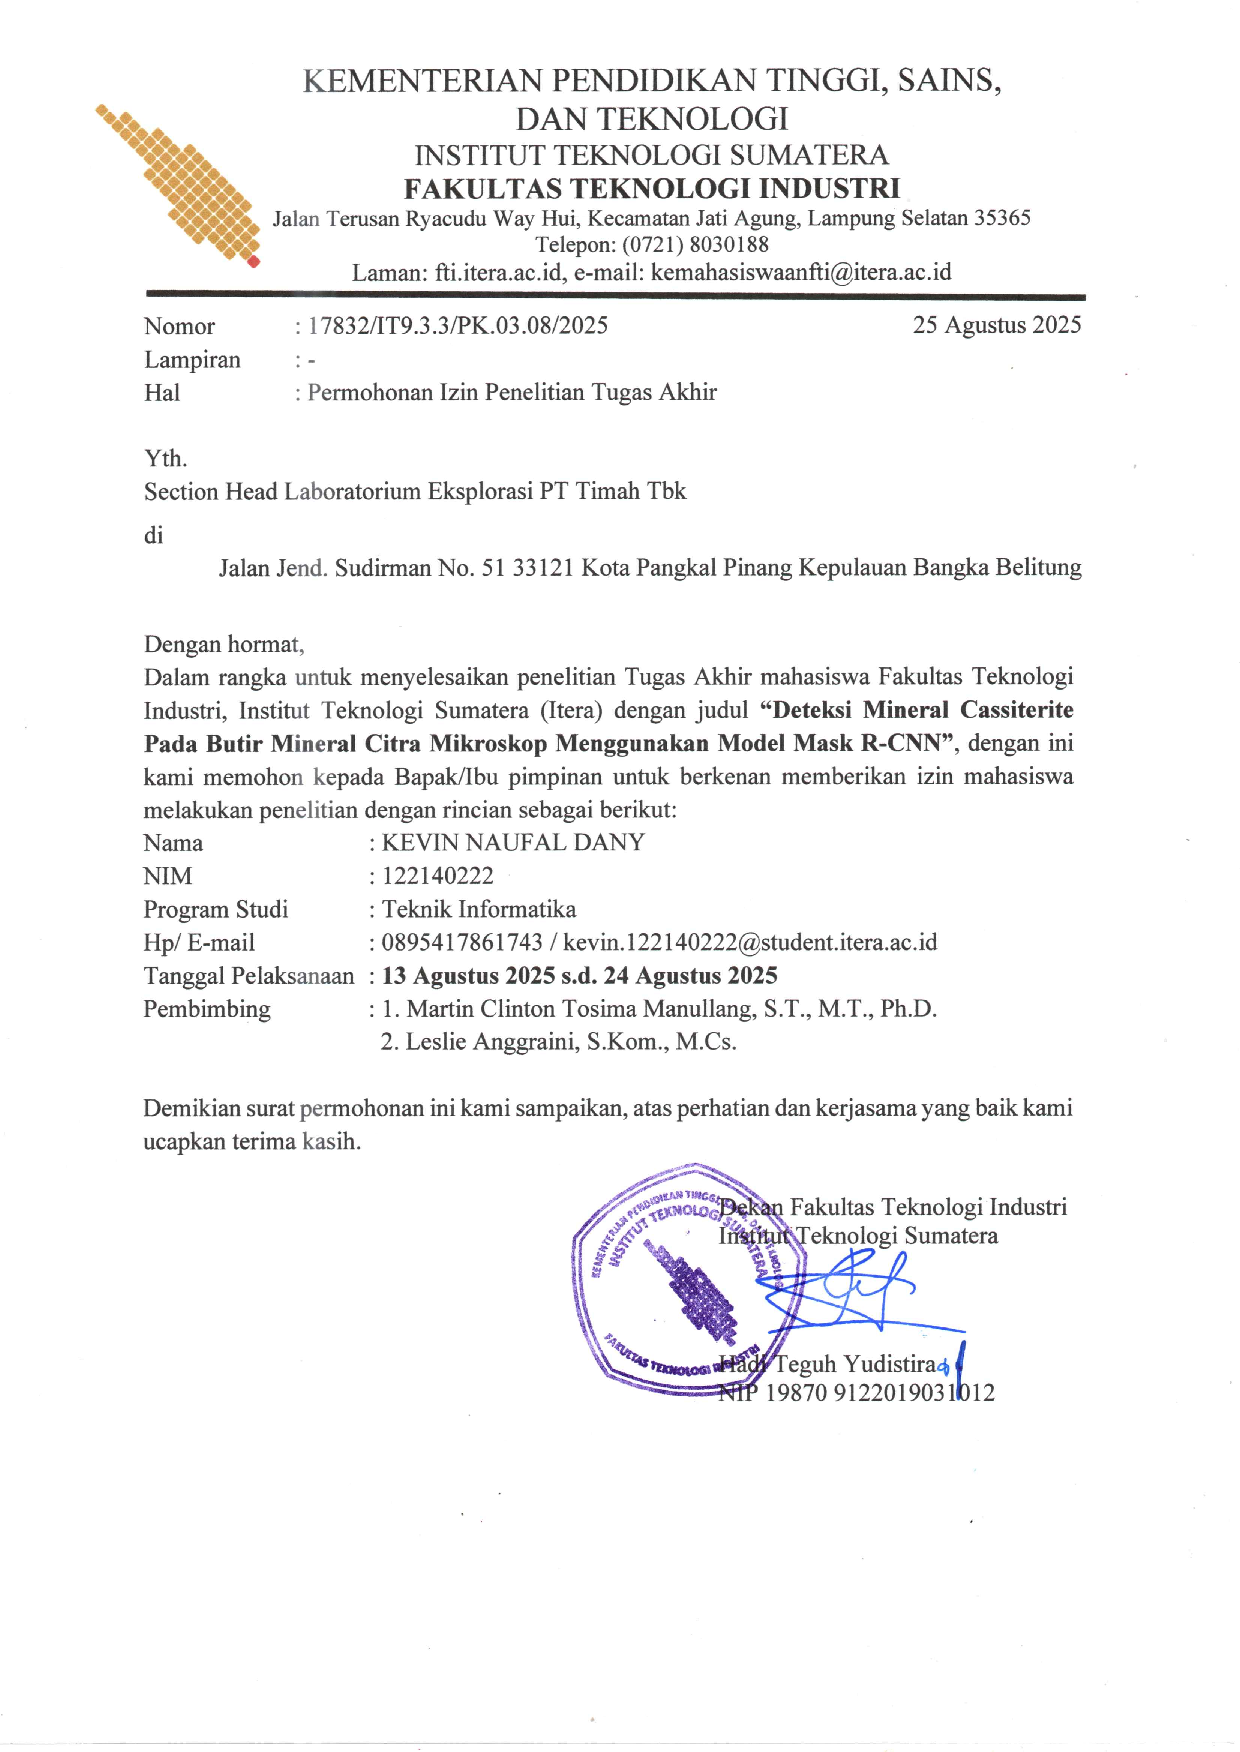
\includegraphics[page=1, width=0.85\textwidth]{doc/surat_izin_penelitian_kevin_pt_timah.pdf}
    \caption{Surat Izin Penelitian Tugas Akhir ke Laboratorium Eksplorasi PT Timah Tbk}
    \label{fig:SuratIzinPenelitian}
\end{figure}

\begin{figure}[H] % Kalau menggunakan H, posisi gambar akan tepat dibawah teks
    \centering
    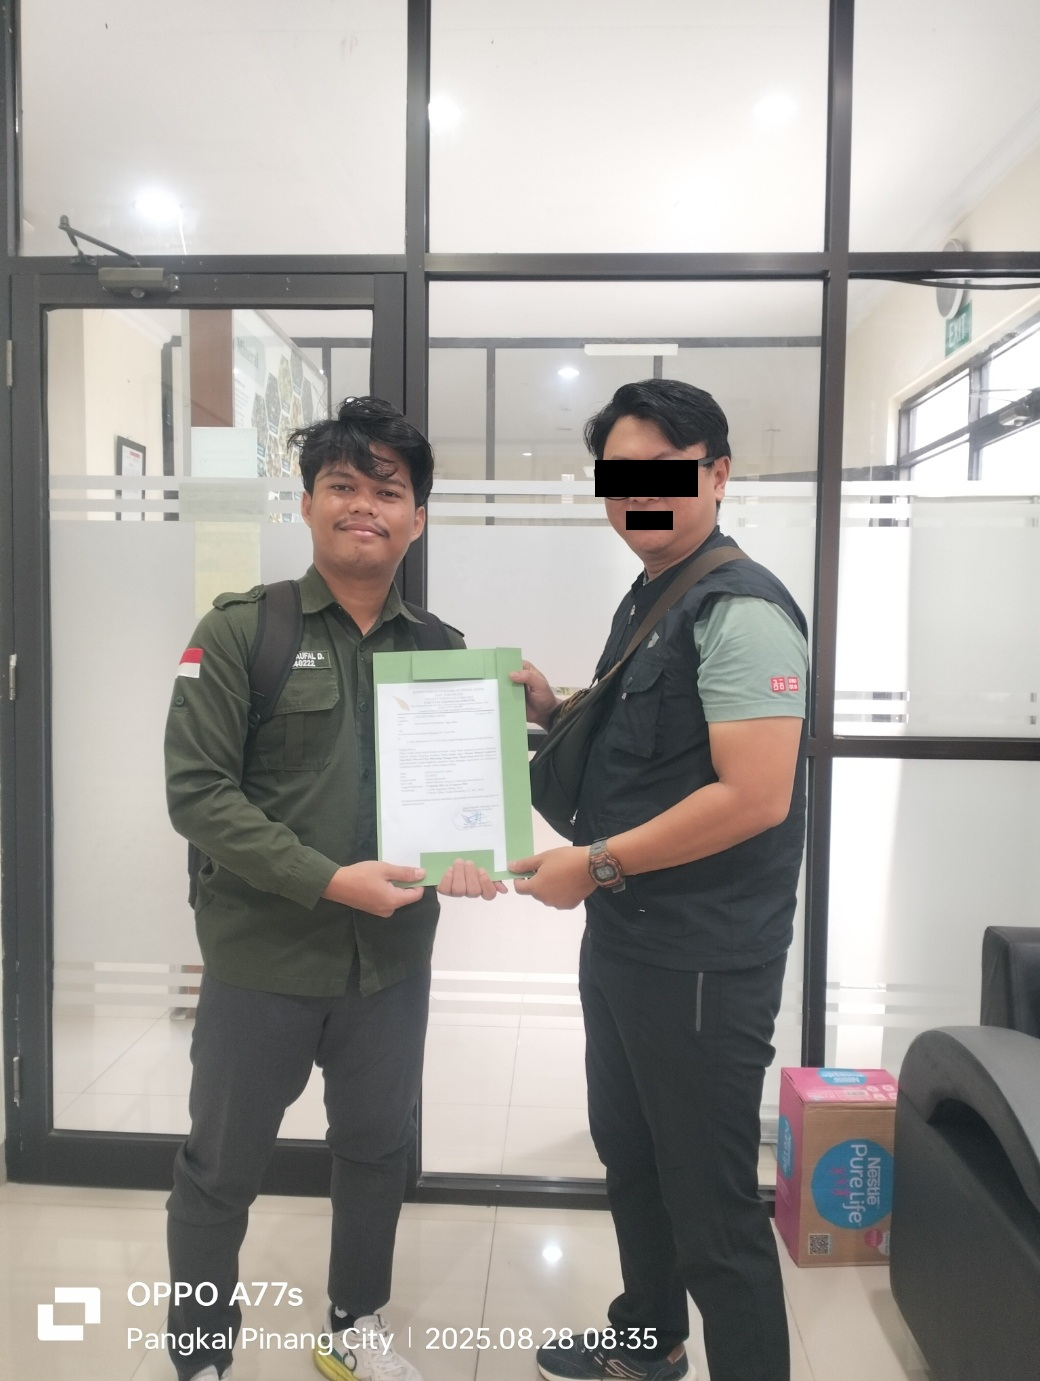
\includegraphics[width=0.85\textwidth]{figure/lampiran/pakMesaSurat.jpg}
    \caption{Surat Pengantar Penelitian}
    \label{fig:PengantarPenelitian}
\end{figure}

\section{Lampiran 2. Dataset} \label{lampiran:Dataset}

\begin{figure}[H] % Kalau menggunakan H, posisi gambar akan tepat dibawah teks
    \centering
    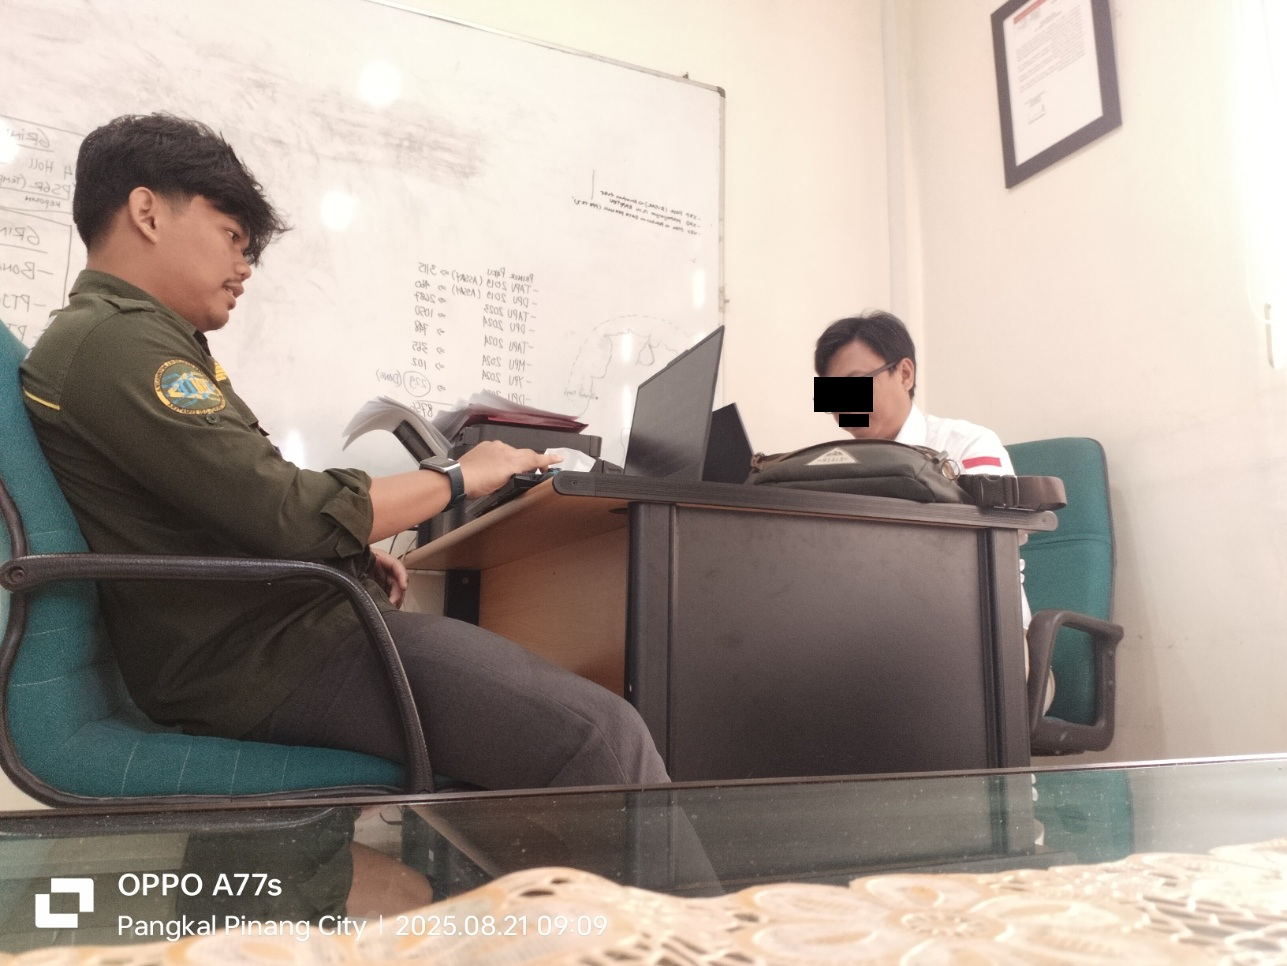
\includegraphics[width=0.85\textwidth]{figure/lampiran/pakMesaData.jpg}
    \caption{Pengumpulan Data}
    \label{fig:PengumpulanData}
\end{figure}


\section{Lampiran 3. Hasil Wawancara} \label{lampiran:Wawancara}
\begin{figure}[H] % Kalau menggunakan H, posisi gambar akan tepat dibawah teks
    \centering
    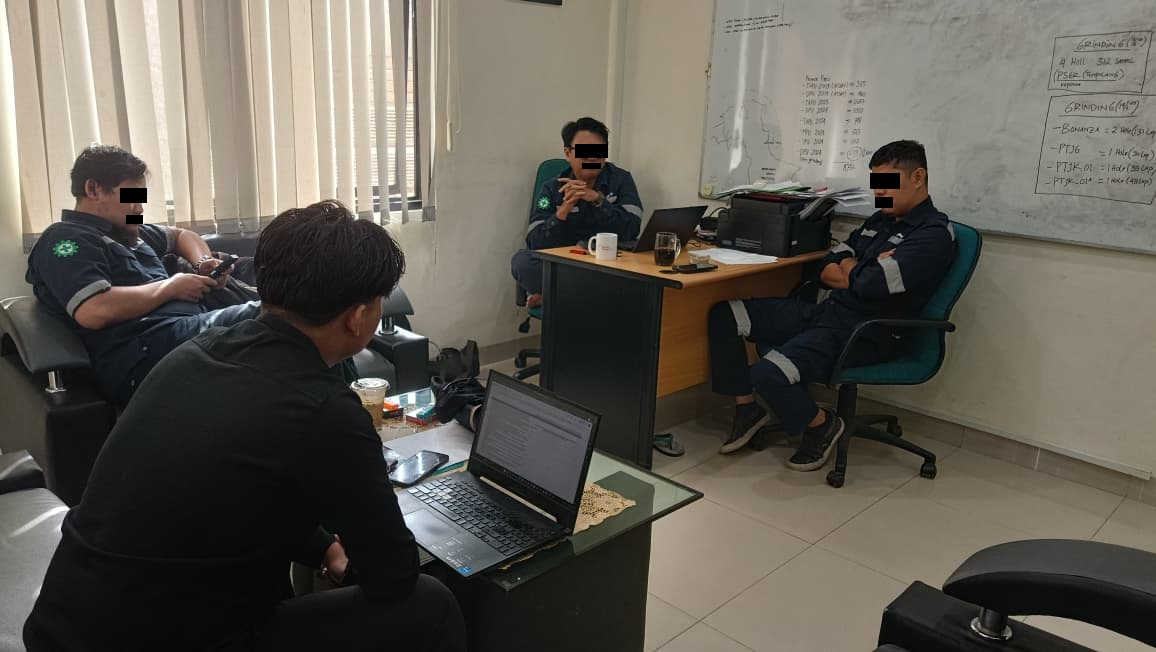
\includegraphics[width=0.85\textwidth]{figure/lampiran/fotoWwc.jpg}
    \caption{Wawancara dengan Bapak Mesa Madestriasa}
    \label{fig:Wawancara}
\end{figure}

{\footnotesize
\begin{longtable}{|p{0.025\textwidth}|p{0.45\textwidth}|p{0.45\textwidth}|}
\caption{List Pertanyaan dan Jawaban dari Hasil Wawancara}
\label{table:wawancara-bijih-timah} \\
\hline
\centering\textbf{No} & \centering\textbf{Pertanyaan} & \centering\arraybackslash\textbf{Jawaban} \\
\hline
\endfirsthead

\hline
\centering\textbf{No} & \centering\textbf{Pertanyaan} & \centering\arraybackslash\textbf{Jawaban} \\
\hline
\endhead

1 &
Di sini saya sedang melakukan penelitian mengenai deteksi bijih timah pada citra microskop menggunakan kecerdasan buatan gitu pak, jadi kasarnya itu membuat suatu program gitu yang dapat mendeteksi dan memprediksi ada berapa dan dimana saja si bijih timah pada suatu citra atau foto microskop tersebut seperti menggunakan Microscope Software, menurut apakah apakah penelitian ini bisa di implementasikan dan apakah menurut bapak ini dapat di implementasikan dalam analisis laboratorium saat ini pak &
Bisa sekali dan sudah ada juga project di sebelum2 nya yang dimana sudah 2 tahun yang lalu juga untuk membuat ai tetapi masih sekitar 50\% akurasi prediksi nya, karena saat ini harus 3 kali bolak balik sampel untuk dalam 1 sampel dan pasti ada faktor subjektivitas, dengan ai bisa mengurangi itu \\
\hline

2 &
Apakah ada standar ukuran bijih timah dalam satuan mesh yang di gunakan untuk analisis labolatorium saat ini &
Standar ukuran kita pakai kalau GCA itu tiga mesh atau 3 fraksi 48, 100 -100 mesh \\
\hline

3 &
Apakah ada karakteristik utama dan standar tertentu biji timah (cassiterite) yang membedakan satu jenis sama jenis lain berdasarkan warna atau bentuk seperti (katalog atau ensiklopedia timah) gitu pak? &
Kalau warna timah itu macam-macam. Ada yang dari mulai coklat, hitam, terus ada merah pun ada. kilap minyak / kilap solar nya yang khusus yang ada di cassiterite, ukuran nya tu ronded sampai sub-ronded tidak ada yang angular tidak ad yang tajam2 gitu, karena suda di masukkan ke mesin lalu mineral akan menggerus dirinya sendiri hingga berukuran ronded sampai sub-ronded, katalog ada tetapi seperti poster hanya seperti buku mengenai macam2 mineral'' \\
\hline

4 &
Apa saja jenis biji timah yang paling sering muncul di sampel bapak, dan apa ciri-cirinya yang dapat di lihat dari segi visual terutama foto? &
Jelas bisa, masing2 daerah mempunyai karakteristik bijih timah nya tersendiri jadi yang sering muncul ya seperti pada sebelumnya. Warnanya ya hitam, warna coklat, Coklat gelap, merah gelap. Kilapnya, kilap minyak. Jadi sering muncul kayak lemak-lemak gitu kalau dimulai mikroskop. istilahnya kayak daging dan serat2 daging gitu \\
\hline

5 &
Dari pengalaman bapak, apa tantangan terbesar dalam mengidentifikasi biji timah secara manual di lab? &
Kalau yang masih baru atau masih belajar biasanya yang tertukar itu antara mineral cassiterite dan ilminite, di karenakan ilminite berwarna hitam dan berkilap karena kalau yang masih baru2 masih belum bisa membedakan kilapnya saja \\
\hline

6 &
Ada nggak pola khusus atau ciri-ciri yang biasanya bapak cari, buat klasifikasi biji timah? &
Kilap minyak itu lah karena kilap minyak di cassiterite sangat khas \\
\hline

7 &
Apakah ada jenis biji timah tertentu yang sering bikin bingung waktu dianalisis pak seperti nemuin yang warnanya mirip banget dengan mineral lain atau memang di modifikasi untuk bijih timah nya (di pilok atau di kasih kecap gitu), seberapa sering di temukan dan gimana cara mengatasinya &
Di karenakan sudah melalui beberapa proses seperti cuci di keringkan sampel itu sebelumnya, sebelum menjadi sebuah sample sebelum di lakukan tim analisis jadi tetep ketahuan walau di pilok pun tetap ketahuan karena kilap minyak cassiterite itu \\
\hline

8 &
Bagaimana proses bapak nyiapin sampel sebelum difoto di mikroskop? &
Untuk penyiapan sampel itu sampel sudah datang clean ke lab karena sudah di keringin jadi langsung di analisa saja, kecuali kalo sampel kasar kita masukkan ke oven atau di goreng dulu jika sudah baru masuk ke lab \\
\hline

9 &
Ada nggak faktor di lab, kayak pencahayaan atau pengaturan mikroskop, yang bisa pengaruhi warna atau tampilan biji timah di foto? &
Sangat berpengaruh, karena data yang saya terima itu juga masih beragam pencahayaannya dan bagusnya itu di dalam 1 mikroskop dan dalam satu ruangan studio jadi pencahayaannya jadi seragam, tpi kalo untuk visual biasa tidak terlalu berpengaruh sekali \\
\hline

10 &
Software apa yang bapak pakai buat motret biji timah di mikroskop? lalu apakah ada format khusus buat gambarnya (.jpg/ .png)? &
Outputnya jpg \\
\hline

11 &
Apakah ukuran 48, 100, -100 Mesh ini punya perbedaan signifikan di lab, misalnya dalam cara pemrosesan atau analisis? &
Ada paling kayak 48 itu kasar, 100 itu sedang lah, -100 halus, kalo semakin kecil semakin membulat, dan misal dia berbeda mesh dalam 1 sampel itu kadang setiap mineral itu menimpa gitu saling menimpa mineral lain \\
\hline

12 &
Kalau saya ingin membuat suatu kecerdasan buatan yang bener-bener akurat, data apa yang menurut bapak wajib banget ada di dataset? &
Dari saya si maunya kasarnya dulu saja untuk menentukan persentase kasiterite nya dulu saja, apakah ai itu bisa atau tidak menemukan mineral kassiterit, jikalau sudah bisa ini sudah good untuk ai nya, persentase yang di maksud itu mengabaikan mineral selain kasiterit seperti semisal ada 100 butir dalam 1 sampel ternyata ada 60 mineral kasiterit berarti itu 60\% gitu untuk mahasiswa seperti itu aja \\
\hline

13 &
Berapa jumlah minimal gambar yang bapak saranin buat dataset biar hasil kecerdasan buatan akurat? &
Untuk data saat ini ada 1046 jadi seharusnya cukup untuk ai ya \\
\hline

\end{longtable}
}


\section{Lampiran 4. Observasi} \label{lampiran:Observasi}
\begin{figure}[H]
    \centering
    % ===== Baris atas =====
    \begin{subfigure}[t]{0.48\textwidth}
        \centering
        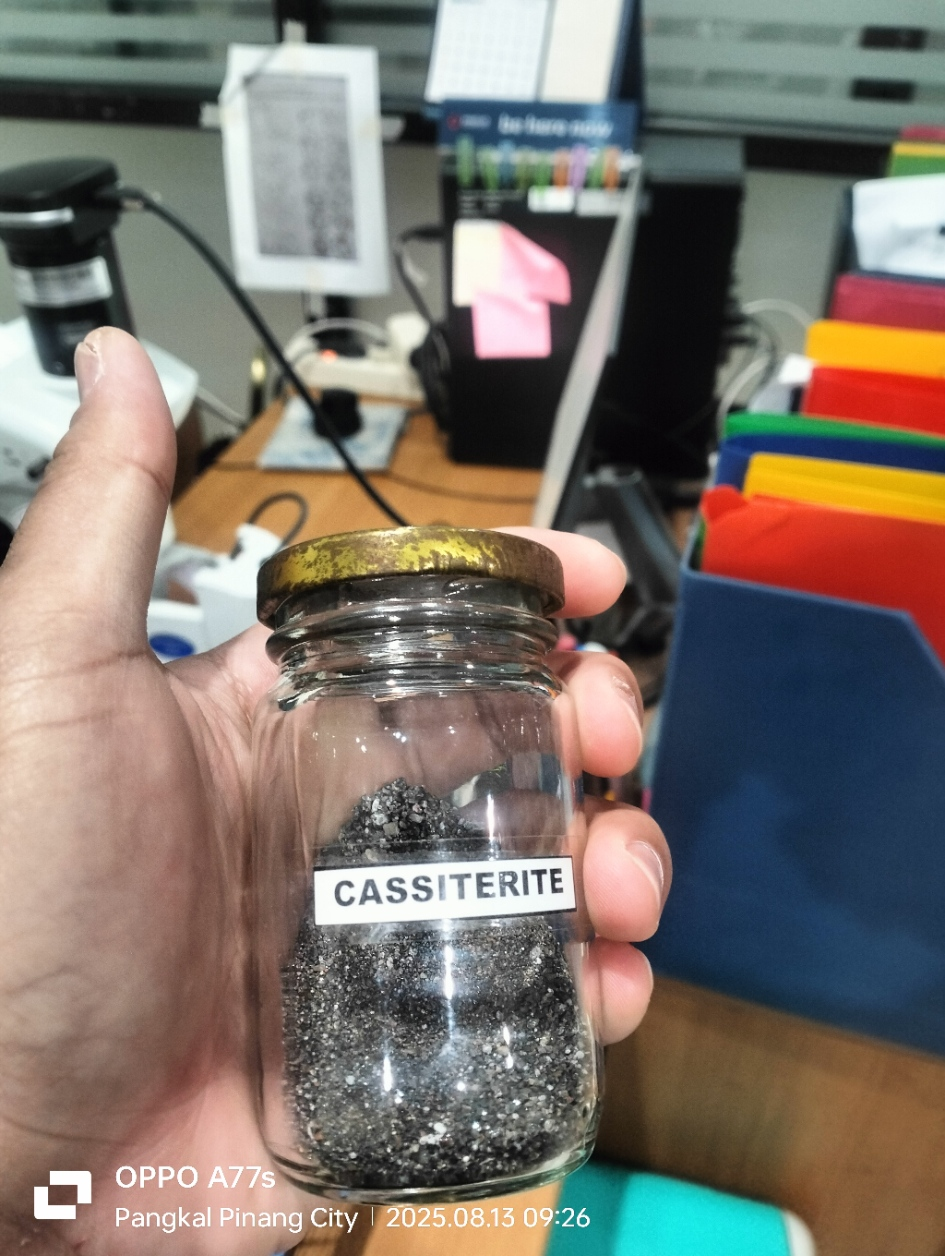
\includegraphics[width=\textwidth]{figure/lampiran/contohMineralCass.jpg}
        \caption{Contoh Mineral Cassiterite}
        \label{fig:ContohMineralCassiterite}
    \end{subfigure}
    \hfill
    \begin{subfigure}[t]{0.48\textwidth}
        \centering
        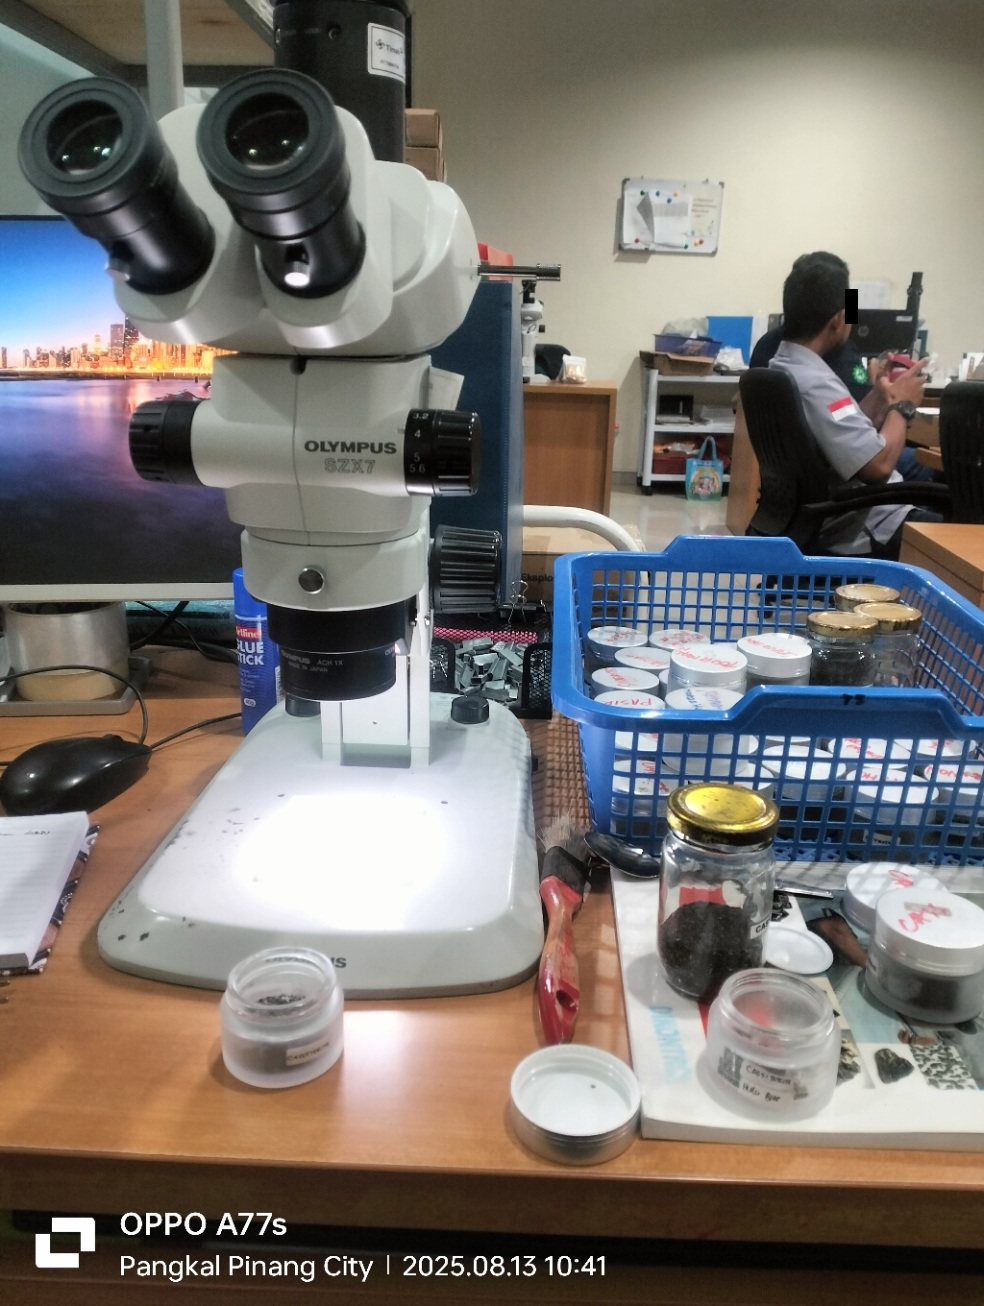
\includegraphics[width=\textwidth]{figure/lampiran/contohMikroskop.jpg}
        \caption{Contoh Mikroskop Trinokuler}
        \label{fig:ContohMikroskopTrinokuler}
    \end{subfigure}

    \vspace{0.4cm}

    % ===== Baris bawah =====
    \begin{subfigure}{0.7\textwidth}
        \centering
        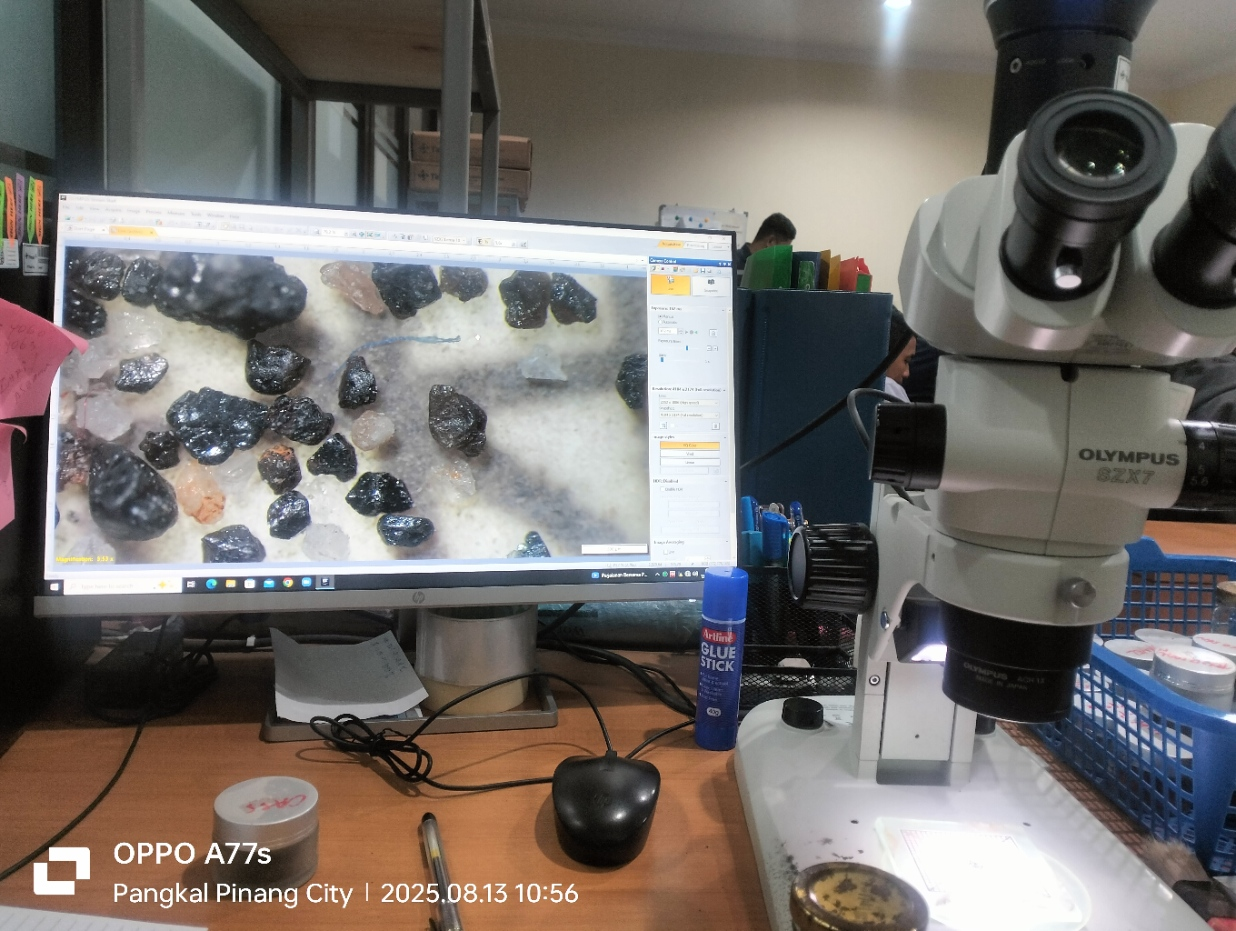
\includegraphics[width=\textwidth]{figure/lampiran/contohHasilCitraMikroskop.jpg}
        \caption{Contoh Hasil Citra Mikroskop}
        \label{fig:ContohHasilCitraMikroskop}
    \end{subfigure}

    \caption{Contoh Mineral Kasiterit, Mikroskop Trinokuler, dan Hasil Citra Mikroskop}
    \label{fig:ContohGabunganMikroskop}
\end{figure}


\begin{figure}[H]
    \centering
    % ===== Baris atas =====
    \begin{subfigure}[t]{0.48\textwidth}
        \centering
        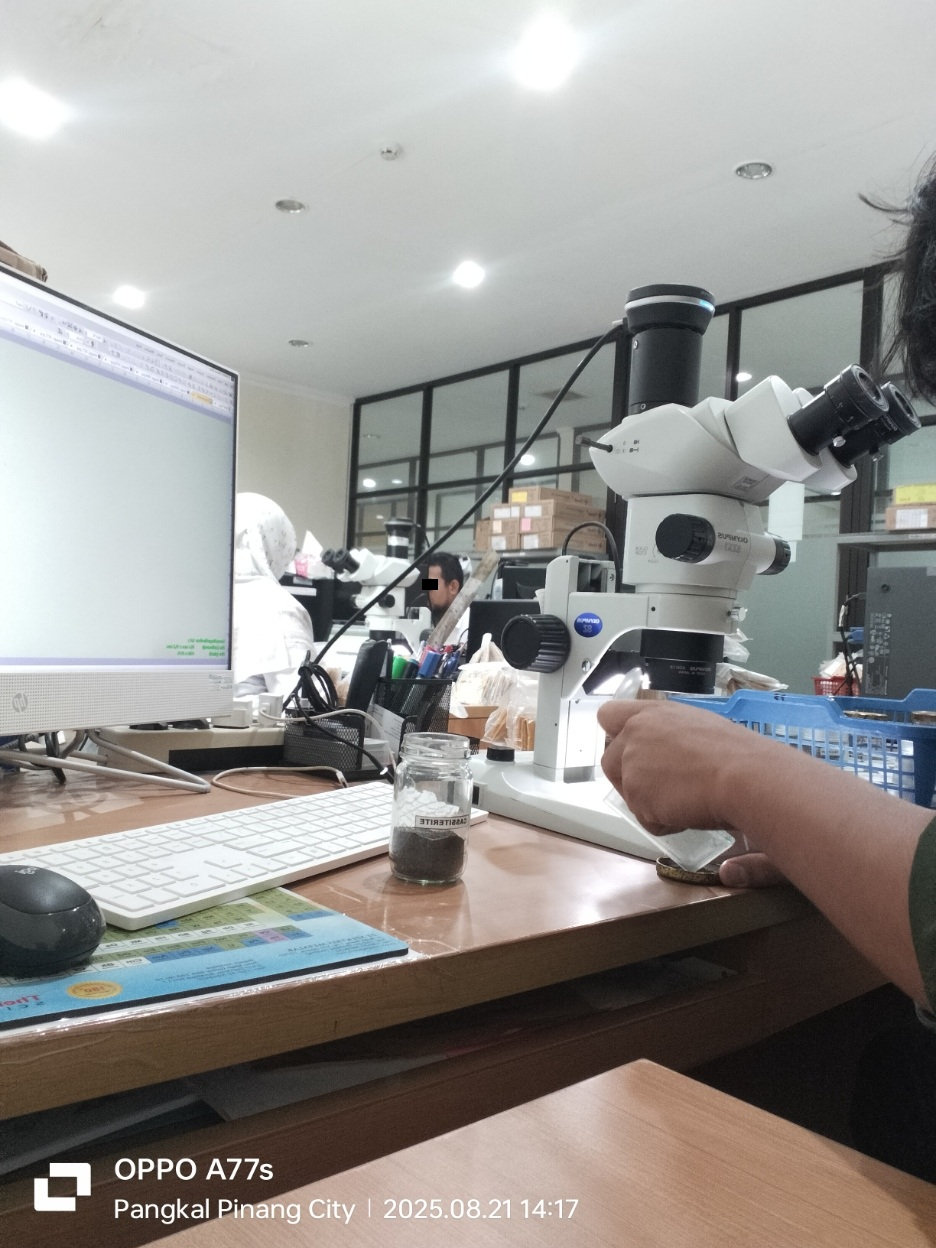
\includegraphics[width=\textwidth]{figure/lampiran/penampangMineral.jpg}
        \caption{Membersihkan Penampang Mineral}
        \label{fig:MembersihkanPenampangMineral}
    \end{subfigure}
    \hfill
    \begin{subfigure}[t]{0.48\textwidth}
        \centering
        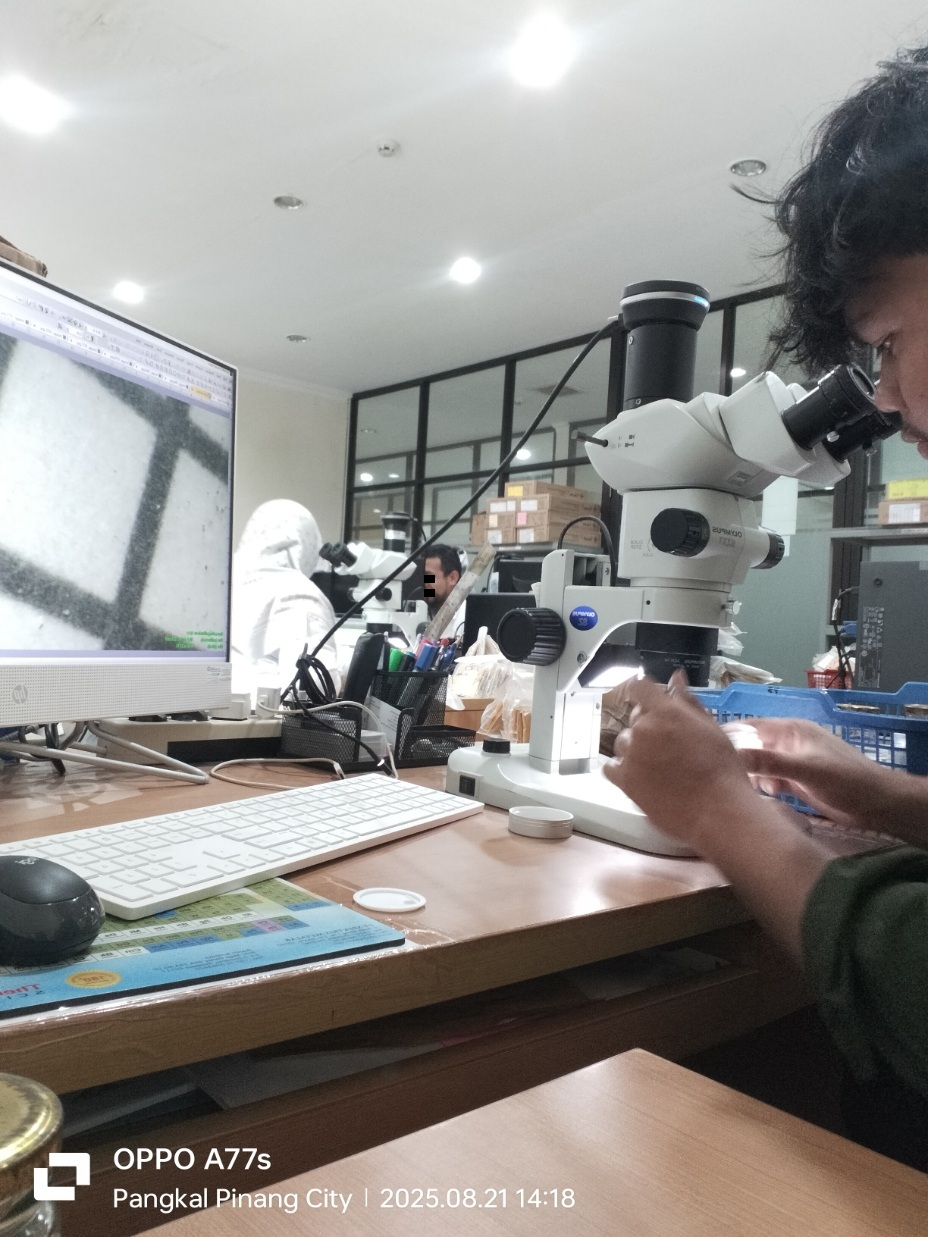
\includegraphics[width=\textwidth]{figure/lampiran/mencobaMenaburiMineralDiPenampang.jpg}
        \caption{Menaburi Mineral Kasiterit di Penampang Mineral}
        \label{fig:MenaburiMineralKasiteritDiPenampang}
    \end{subfigure}

    \vspace{0.4cm}

    % ===== Baris bawah =====
    \begin{subfigure}{0.6\textwidth}
        \centering
        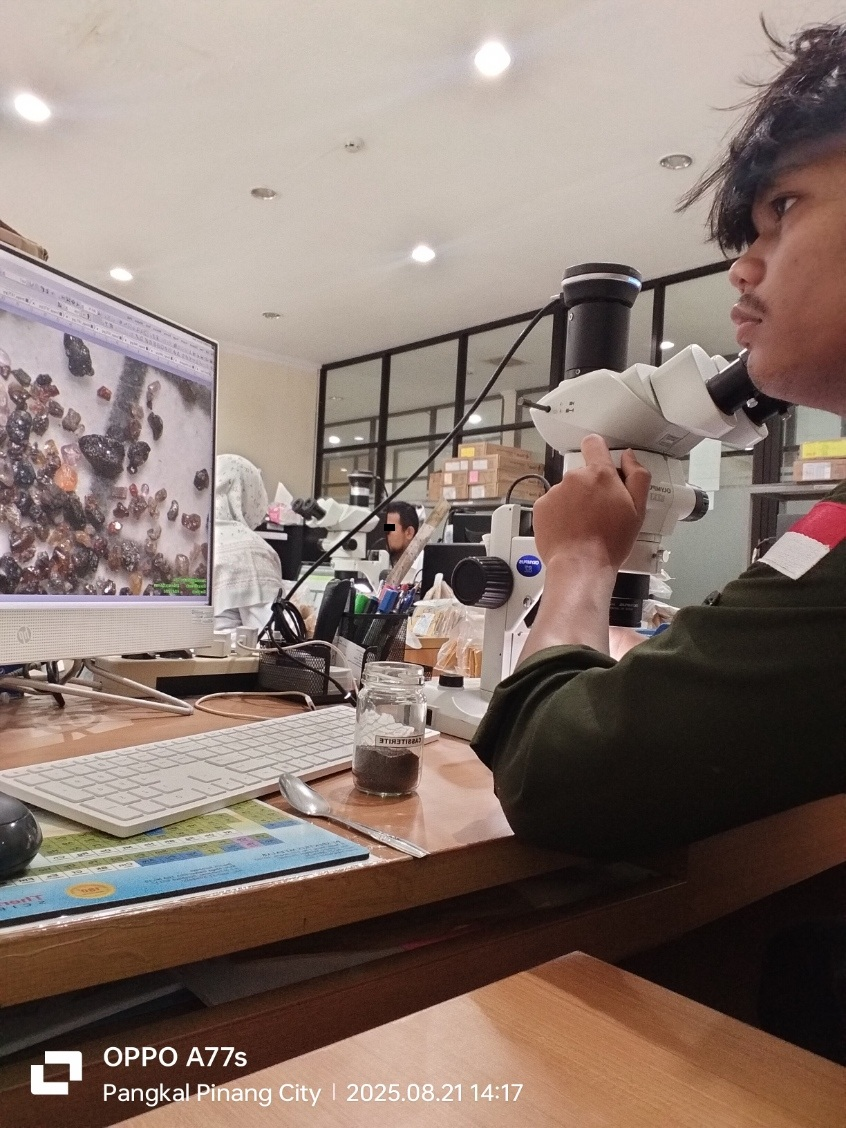
\includegraphics[width=\textwidth]{figure/lampiran/mencobaMikroskop.jpg}
        \caption{Melakukan Pengamatan Terhadap Citra Butiran Mineral Kasiterit dan Mineral Ikutan Lainnya untuk Memahami Karakteristik Secara Visual Menggunakan Mikroskop Trinokuler}
        \label{fig:MenggunakanMikroskopTrinokuler}
    \end{subfigure}

    \caption{Tahapan Persiapan dan Pengamatan Mineral Kasiterit Menggunakan Mikroskop Trinokuler}
    \label{fig:ProsesPengamatanMineralKasiterit}
\end{figure}


\section{Lampiran 5. Hasil Evaluasi Model} \label{lampiran:HasilEvaluasiModel}
\subsection*{Variasi 1 \textit{Mask} R-CNN ResNet50 FPN V1 + \textit{Amodal} + SGD}
\begin{figure}[H]
    \centering
    \fbox{\begin{minipage}{0.95\textwidth}
        \centering
        \begin{tabular}{cc}
            
\includegraphics[width=0.45\textwidth]{figure/lampiran/lampiran_eval/resnet50_fpn_v1_amodal_sgd_lr0.01/fold1/loss_fold1.png} &
            
\includegraphics[width=0.45\textwidth]{figure/lampiran/lampiran_eval/resnet50_fpn_v1_amodal_sgd_lr0.01/fold1/mean_metrics_comparison_fold1.png} \\[0.5em]
            
\includegraphics[width=0.45\textwidth]{figure/lampiran/lampiran_eval/resnet50_fpn_v1_amodal_sgd_lr0.01/fold2/loss_fold2.png} &
            
\includegraphics[width=0.45\textwidth]{figure/lampiran/lampiran_eval/resnet50_fpn_v1_amodal_sgd_lr0.01/fold2/mean_metrics_comparison_fold2.png} \\[0.5em]
            
\includegraphics[width=0.45\textwidth]{figure/lampiran/lampiran_eval/resnet50_fpn_v1_amodal_sgd_lr0.01/fold3/loss_fold3.png} &
            
\includegraphics[width=0.45\textwidth]{figure/lampiran/lampiran_eval/resnet50_fpn_v1_amodal_sgd_lr0.01/fold3/mean_metrics_comparison_fold3.png} \\[0.5em]
            
\includegraphics[width=0.45\textwidth]{figure/lampiran/lampiran_eval/resnet50_fpn_v1_amodal_sgd_lr0.01/fold4/loss_fold4.png} &
            
\includegraphics[width=0.45\textwidth]{figure/lampiran/lampiran_eval/resnet50_fpn_v1_amodal_sgd_lr0.01/fold4/mean_metrics_comparison_fold4.png} \\[0.5em]
            
\includegraphics[width=0.45\textwidth]{figure/lampiran/lampiran_eval/resnet50_fpn_v1_amodal_sgd_lr0.01/fold5/loss_fold5.png} &
            
\includegraphics[width=0.45\textwidth]{figure/lampiran/lampiran_eval/resnet50_fpn_v1_amodal_sgd_lr0.01/fold5/mean_metrics_comparison_fold5.png} \\
        \end{tabular}
    \end{minipage}}
    \caption{Hasil Evaluasi Model Variasi 1 \textit{Mask} R-CNN ResNet50 FPN V1 + \textit{Amodal} + SGD}
    \label{fig:HasilEvaluasiModel1}
\end{figure}

\subsection*{Variasi 2 \textit{Mask} R-CNN ResNet50 FPN V1 + \textit{Amodal} + Adam}
\begin{figure}[H]
    \centering
    \fbox{\begin{minipage}{0.95\textwidth}
        \centering
        \begin{tabular}{cc}
            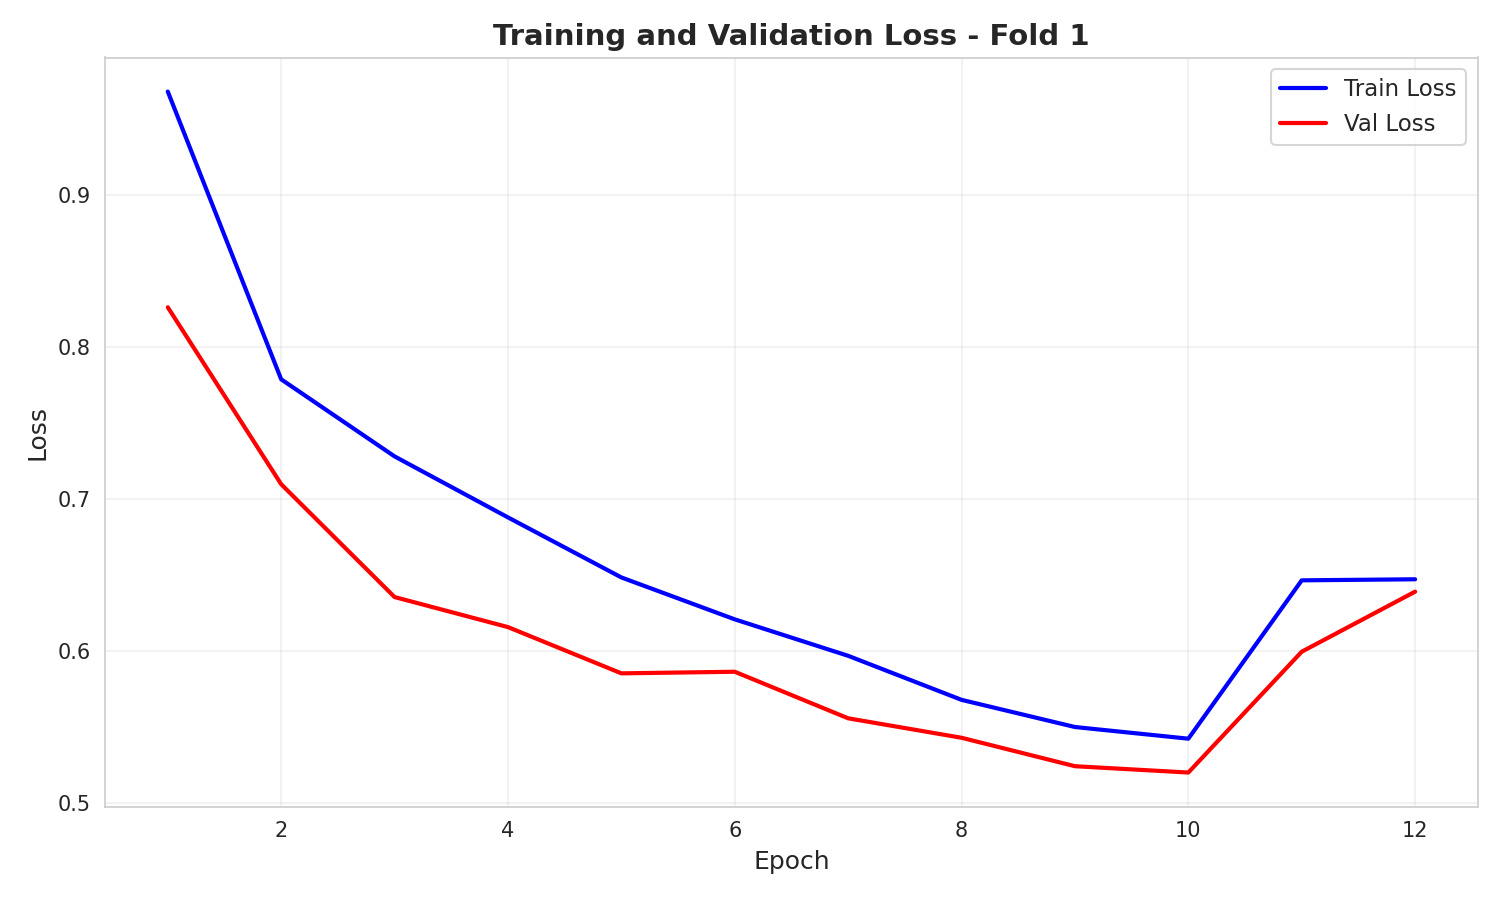
\includegraphics[width=0.45\textwidth]{figure/lampiran/lampiran_eval/resnet50_fpn_v1_amodal_adam_lr1e-04/fold1/loss_fold1.png} &
            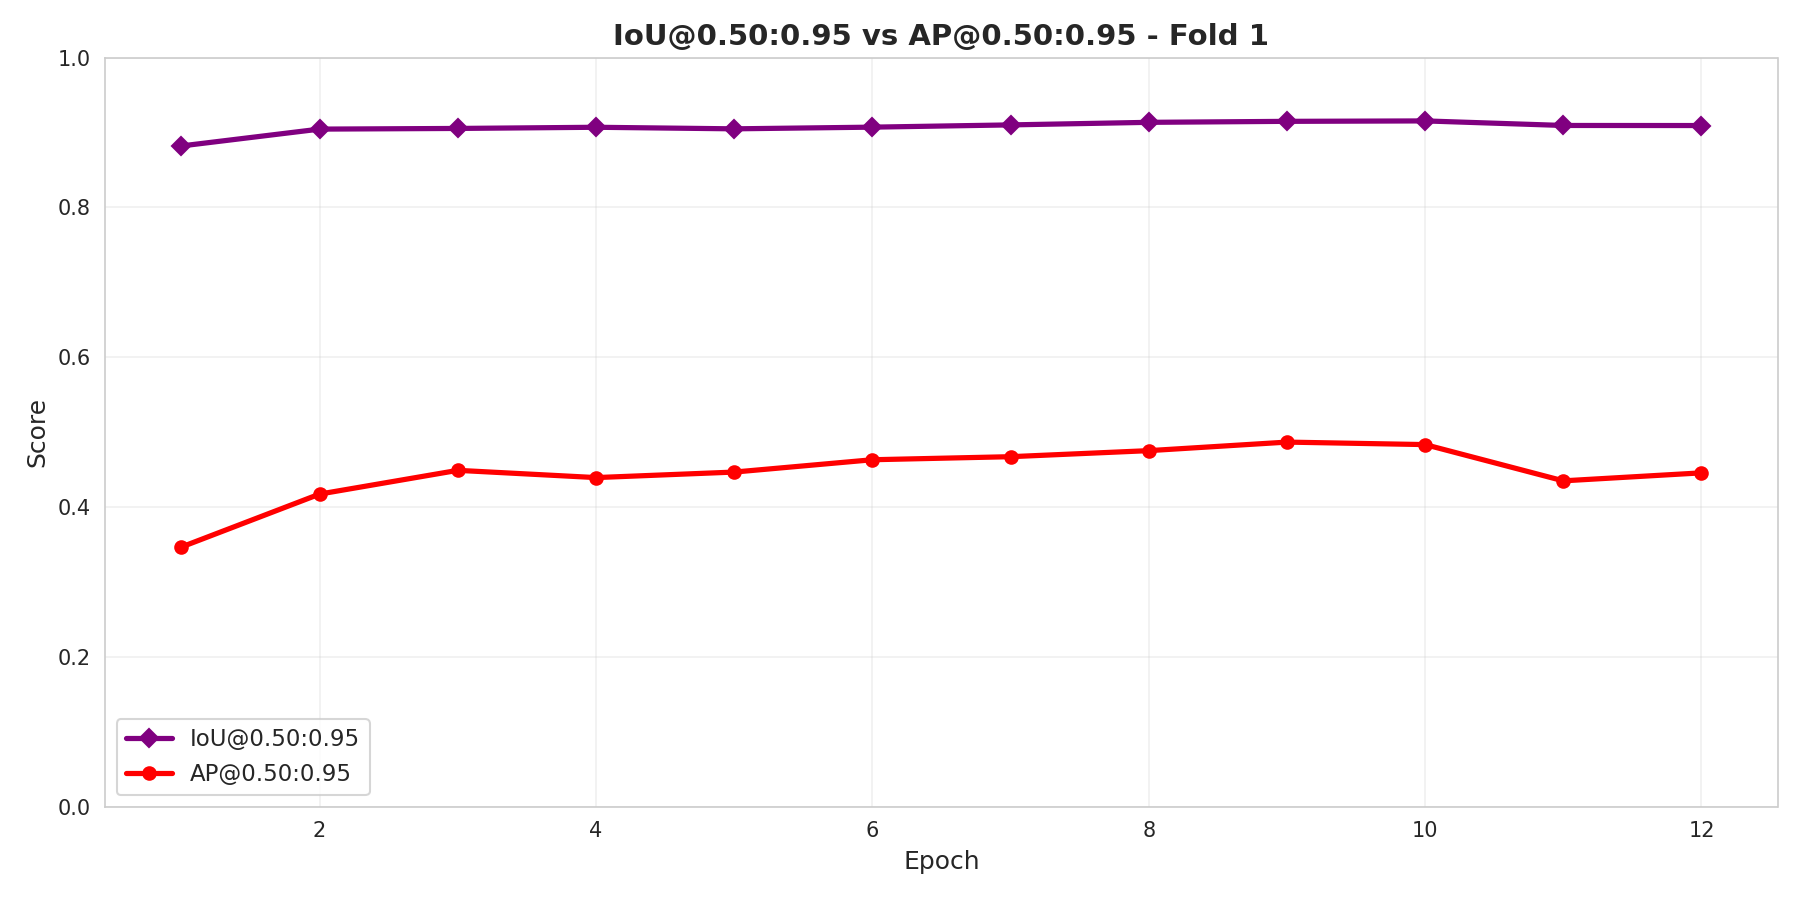
\includegraphics[width=0.45\textwidth]{figure/lampiran/lampiran_eval/resnet50_fpn_v1_amodal_adam_lr1e-04/fold1/mean_metrics_comparison_fold1.png} \\[0.5em]
            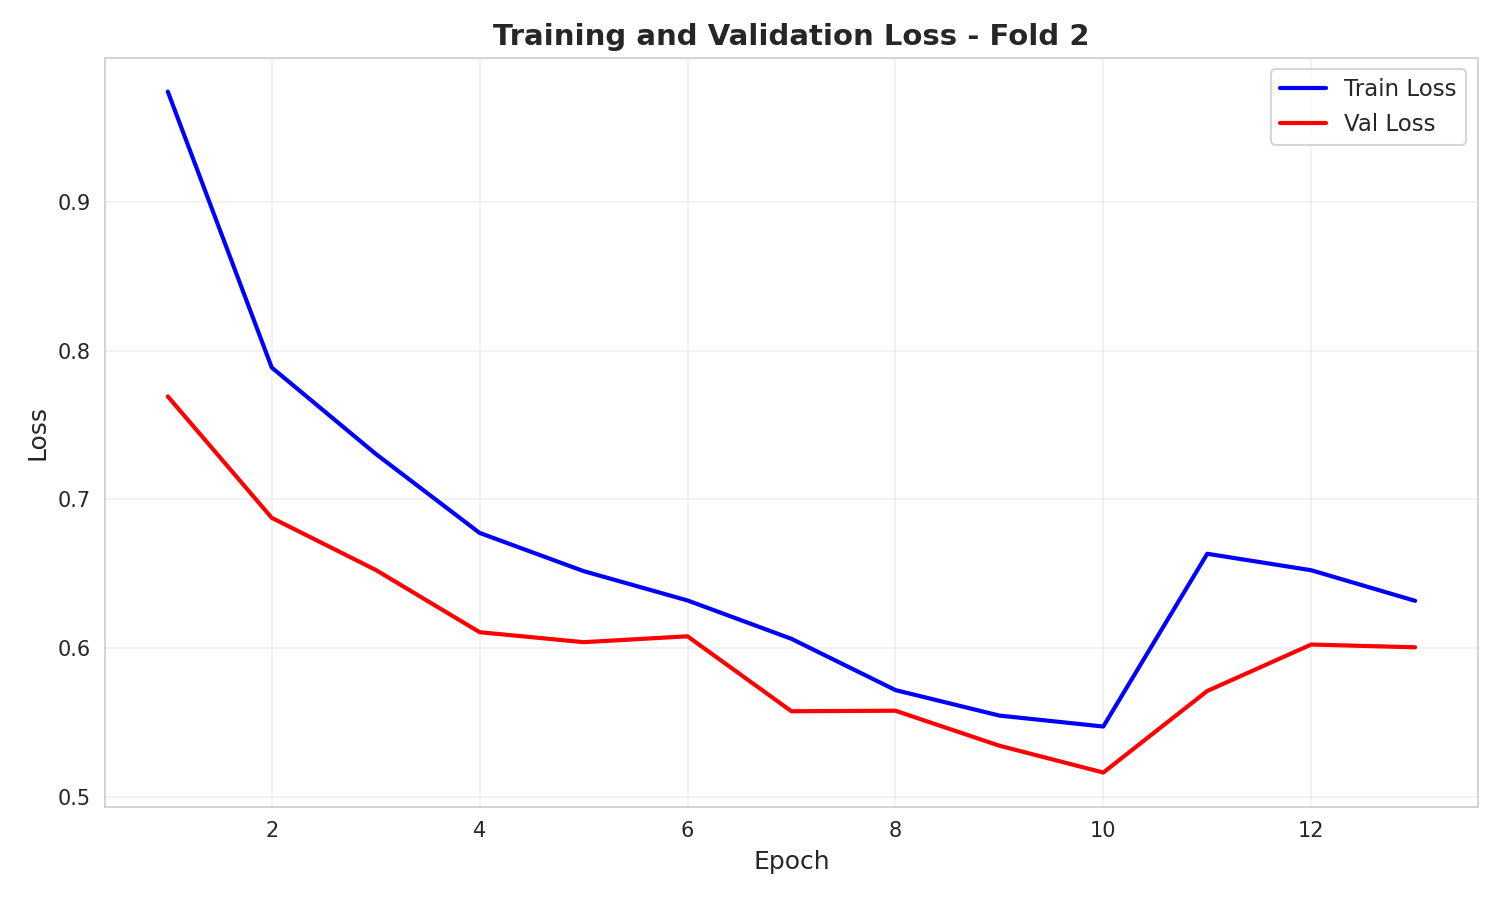
\includegraphics[width=0.45\textwidth]{figure/lampiran/lampiran_eval/resnet50_fpn_v1_amodal_adam_lr1e-04/fold2/loss_fold2.png} &
            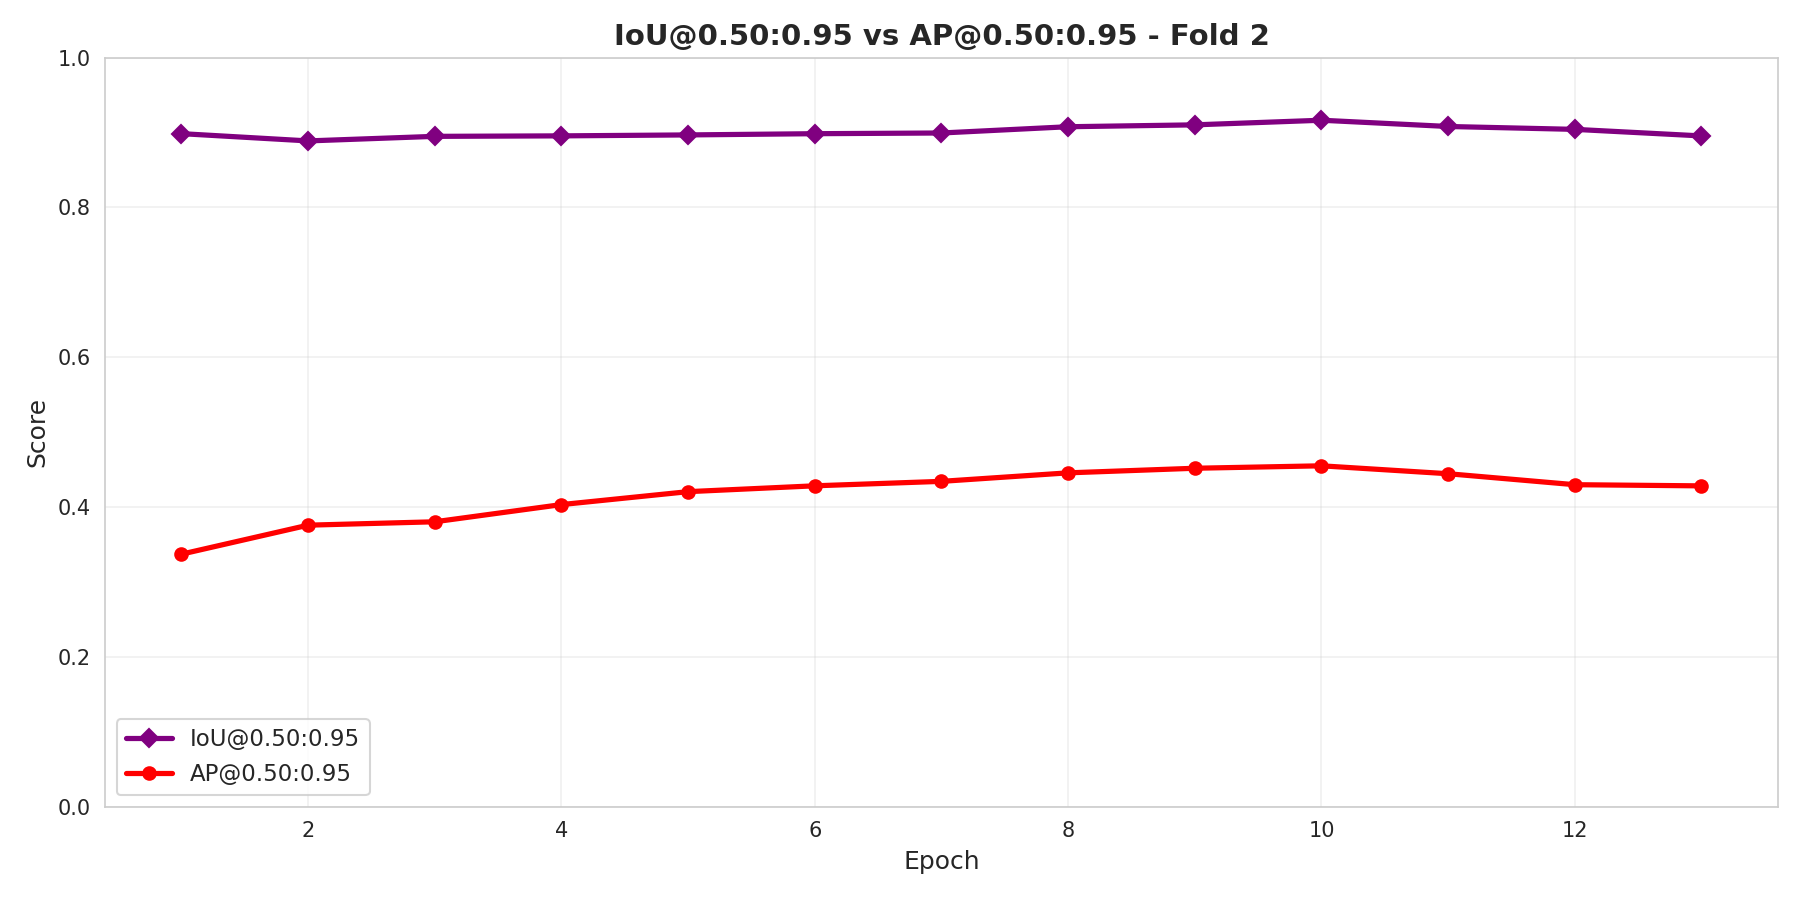
\includegraphics[width=0.45\textwidth]{figure/lampiran/lampiran_eval/resnet50_fpn_v1_amodal_adam_lr1e-04/fold2/mean_metrics_comparison_fold2.png} \\[0.5em]
            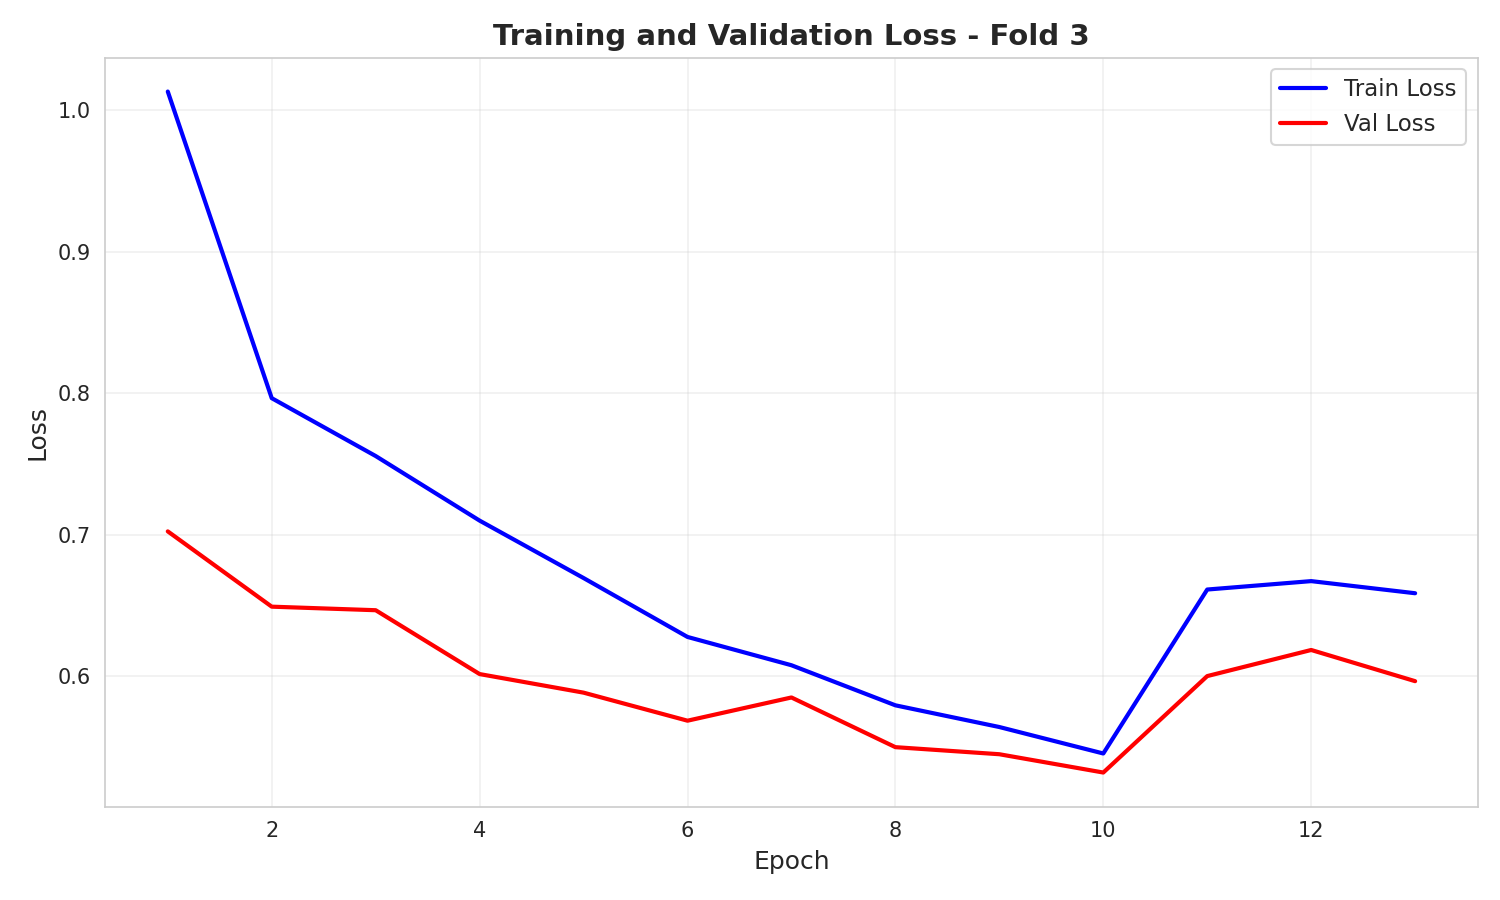
\includegraphics[width=0.45\textwidth]{figure/lampiran/lampiran_eval/resnet50_fpn_v1_amodal_adam_lr1e-04/fold3/loss_fold3.png} &
            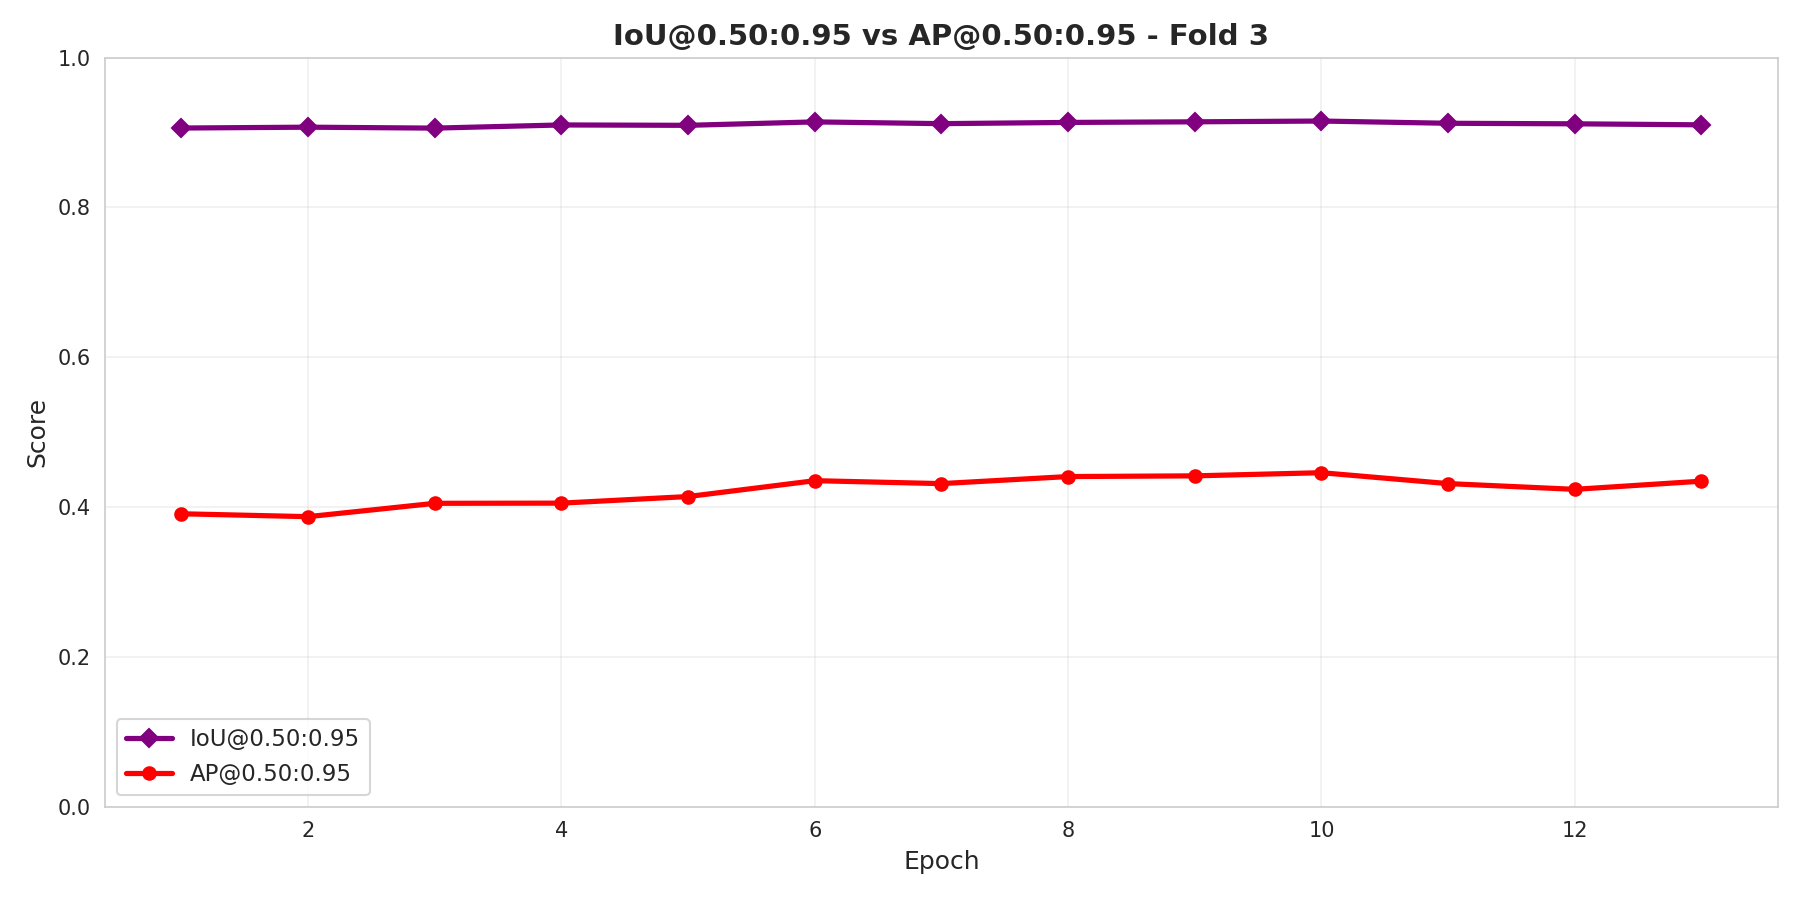
\includegraphics[width=0.45\textwidth]{figure/lampiran/lampiran_eval/resnet50_fpn_v1_amodal_adam_lr1e-04/fold3/mean_metrics_comparison_fold3.png} \\[0.5em]
            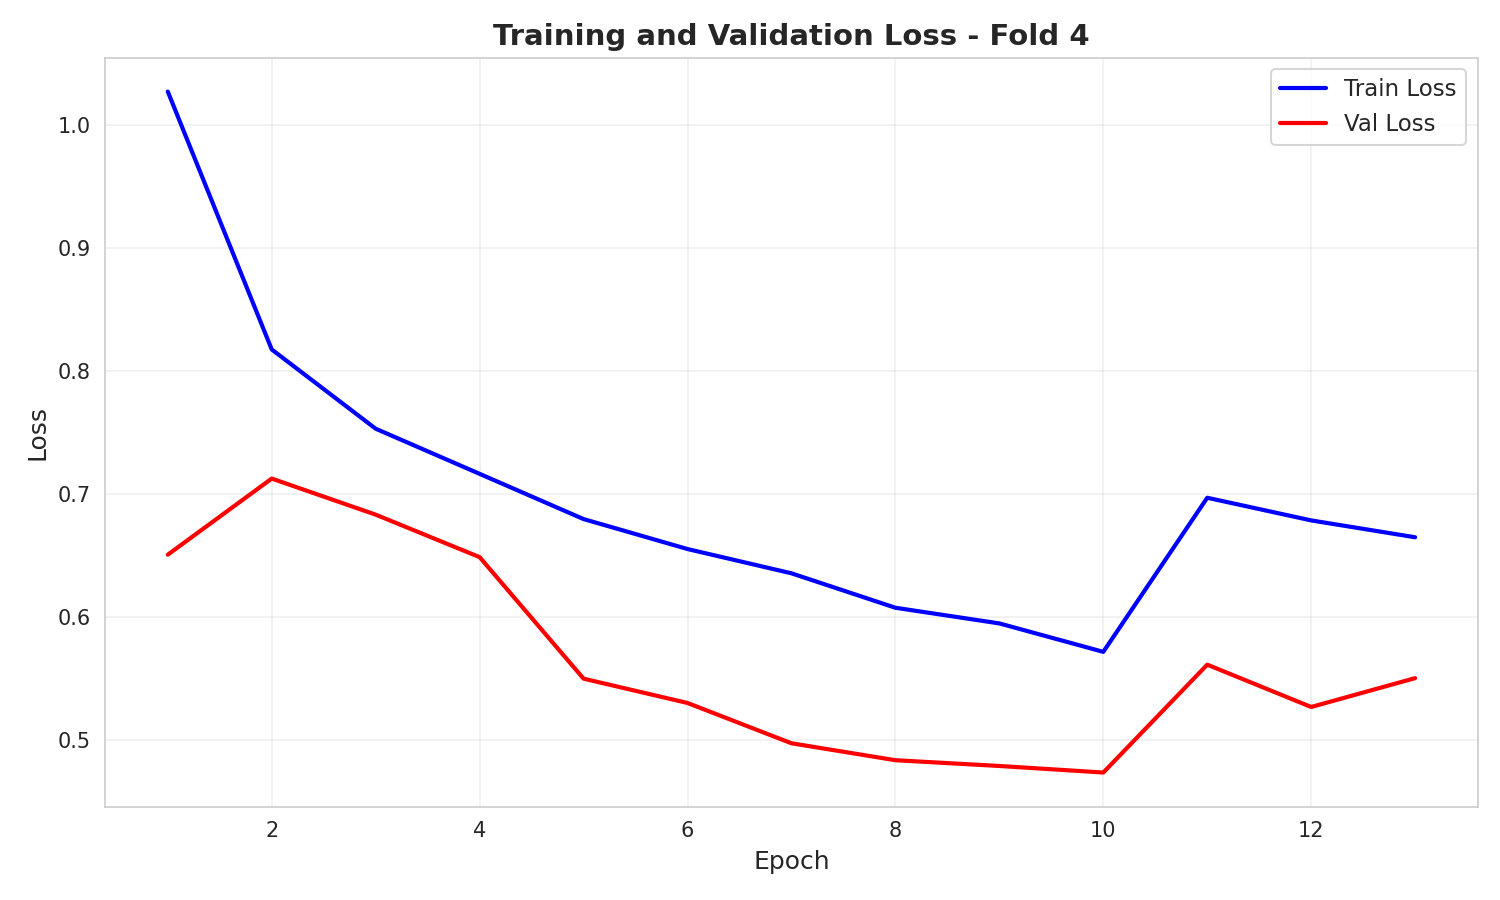
\includegraphics[width=0.45\textwidth]{figure/lampiran/lampiran_eval/resnet50_fpn_v1_amodal_adam_lr1e-04/fold4/loss_fold4.png} &
            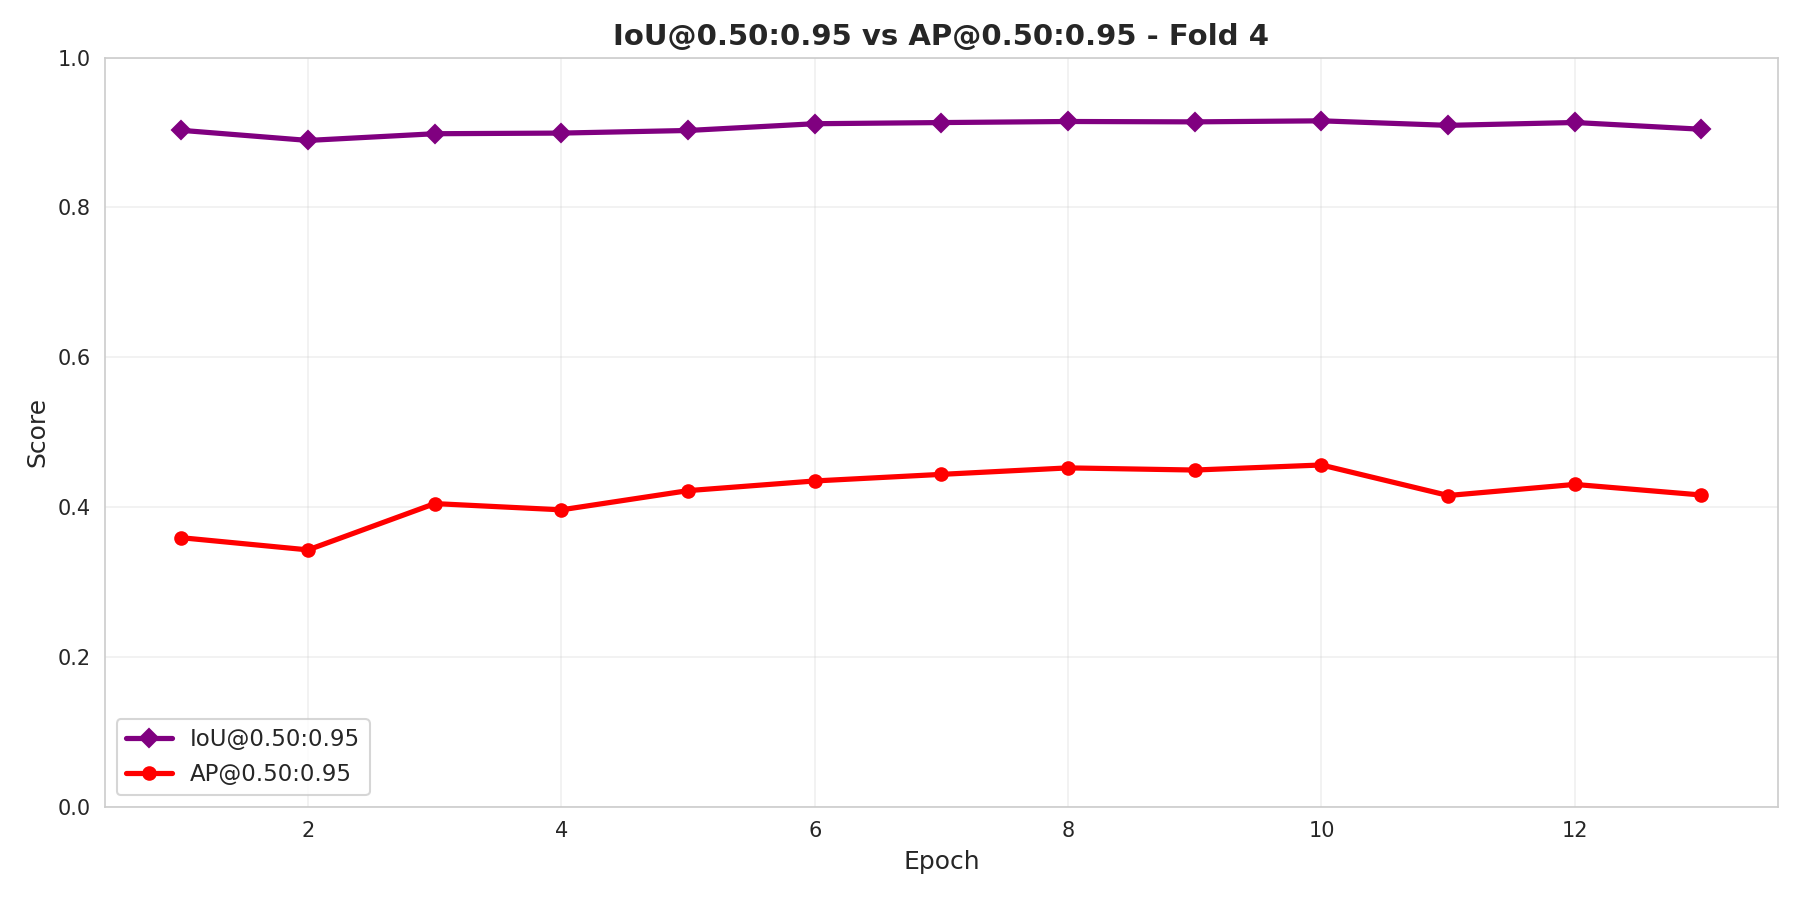
\includegraphics[width=0.45\textwidth]{figure/lampiran/lampiran_eval/resnet50_fpn_v1_amodal_adam_lr1e-04/fold4/mean_metrics_comparison_fold4.png} \\[0.5em]
            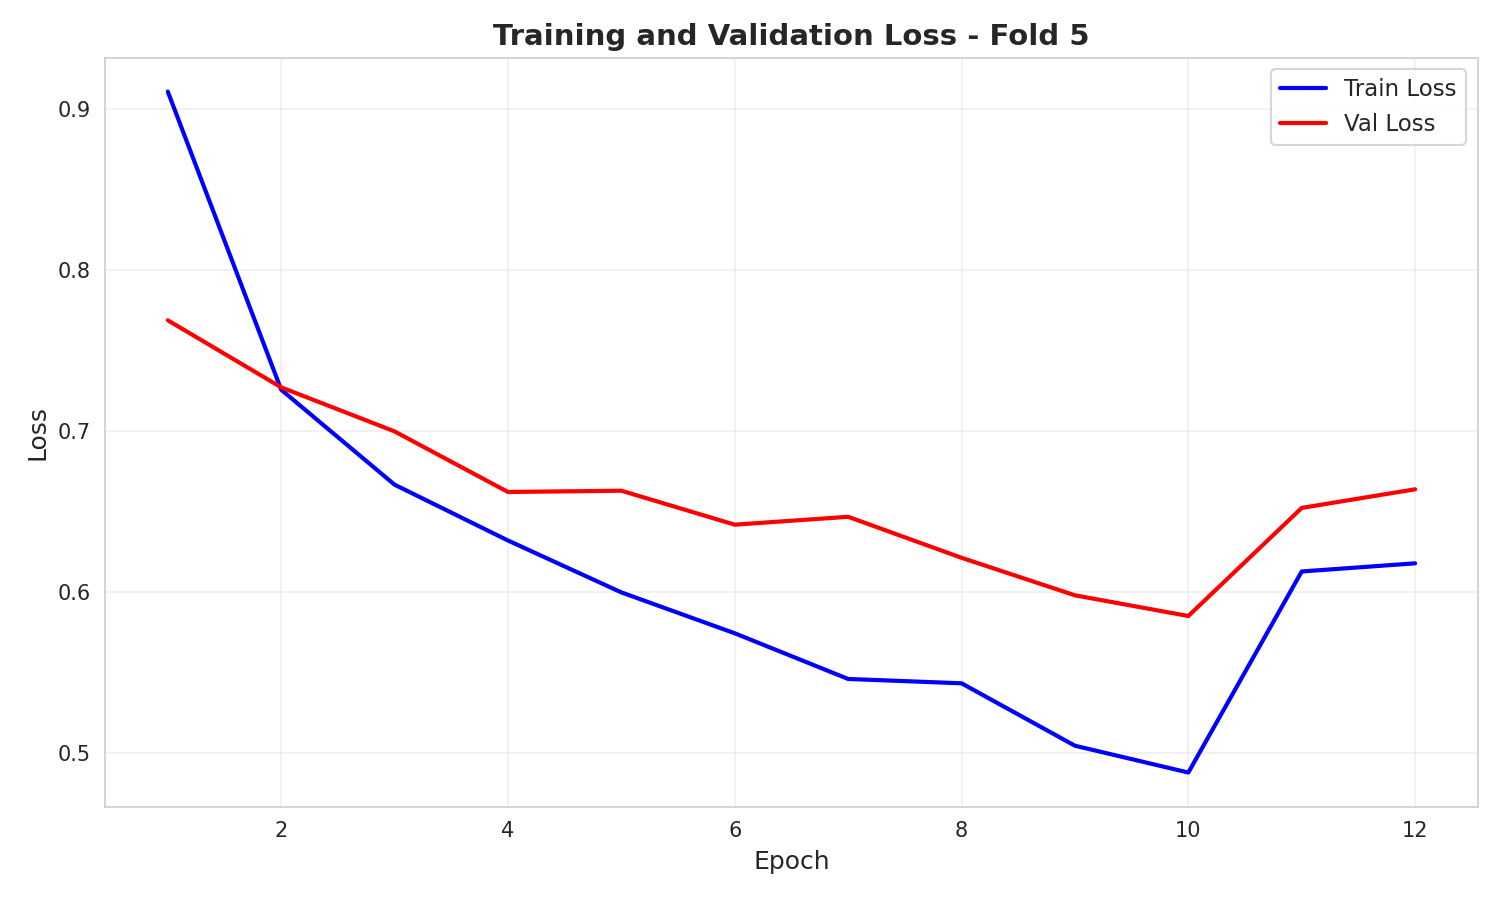
\includegraphics[width=0.45\textwidth]{figure/lampiran/lampiran_eval/resnet50_fpn_v1_amodal_adam_lr1e-04/fold5/loss_fold5.png} &
            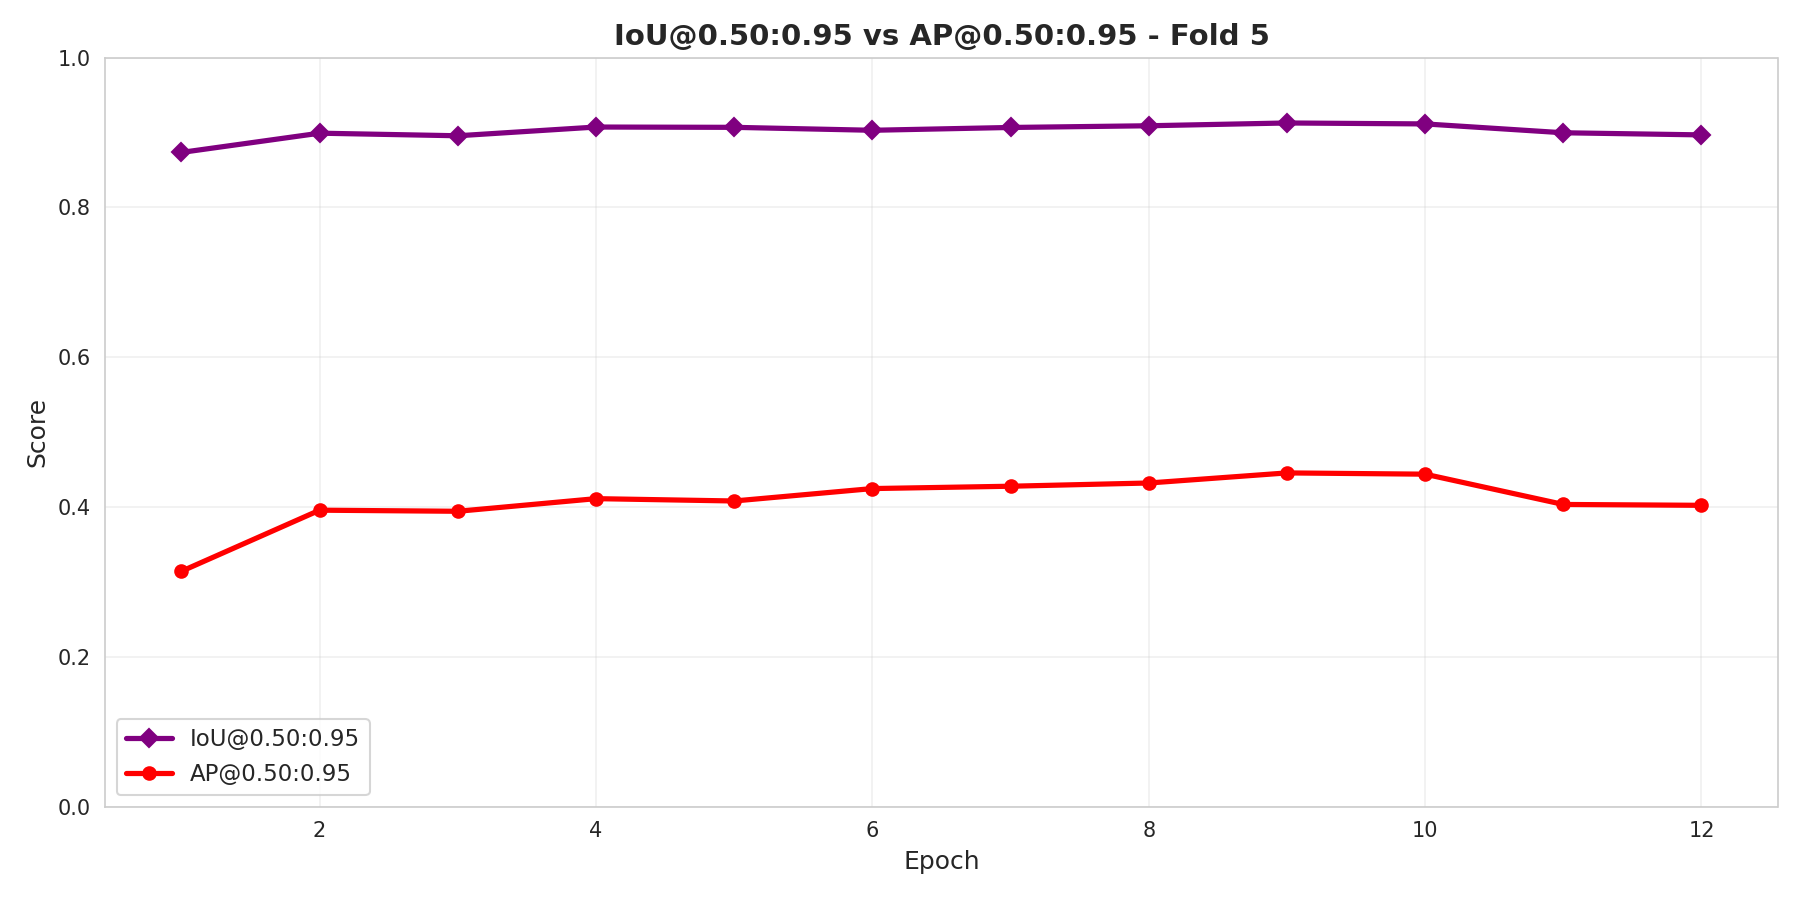
\includegraphics[width=0.45\textwidth]{figure/lampiran/lampiran_eval/resnet50_fpn_v1_amodal_adam_lr1e-04/fold5/mean_metrics_comparison_fold5.png} \\
        \end{tabular}
    \end{minipage}}
    \caption{Hasil Evaluasi Model Variasi 2 \textit{Mask} R-CNN ResNet50 FPN V1 + \textit{Amodal} + Adam}
    \label{fig:HasilEvaluasiModel2}
\end{figure}

\subsection*{Variasi 3 \textit{Mask} R-CNN ResNet50 FPN V2 + \textit{Standard} + SGD}
\begin{figure}[H]
    \centering
    \fbox{\begin{minipage}{0.95\textwidth}
        \centering
        \begin{tabular}{cc}
            
\includegraphics[width=0.45\textwidth]{figure/lampiran/lampiran_eval/resnet50_fpn_v2_standard_sgd_lr0.01/fold1/loss_fold1.png} &
            
\includegraphics[width=0.45\textwidth]{figure/lampiran/lampiran_eval/resnet50_fpn_v2_standard_sgd_lr0.01/fold1/mean_metrics_comparison_fold1.png} \\[0.5em]
            
\includegraphics[width=0.45\textwidth]{figure/lampiran/lampiran_eval/resnet50_fpn_v2_standard_sgd_lr0.01/fold2/loss_fold2.png} &
            
\includegraphics[width=0.45\textwidth]{figure/lampiran/lampiran_eval/resnet50_fpn_v2_standard_sgd_lr0.01/fold2/mean_metrics_comparison_fold2.png} \\[0.5em]
            
\includegraphics[width=0.45\textwidth]{figure/lampiran/lampiran_eval/resnet50_fpn_v2_standard_sgd_lr0.01/fold3/loss_fold3.png} &
            
\includegraphics[width=0.45\textwidth]{figure/lampiran/lampiran_eval/resnet50_fpn_v2_standard_sgd_lr0.01/fold3/mean_metrics_comparison_fold3.png} \\[0.5em]
            
\includegraphics[width=0.45\textwidth]{figure/lampiran/lampiran_eval/resnet50_fpn_v2_standard_sgd_lr0.01/fold4/loss_fold4.png} &
            
\includegraphics[width=0.45\textwidth]{figure/lampiran/lampiran_eval/resnet50_fpn_v2_standard_sgd_lr0.01/fold4/mean_metrics_comparison_fold4.png} \\[0.5em]
            
\includegraphics[width=0.45\textwidth]{figure/lampiran/lampiran_eval/resnet50_fpn_v2_standard_sgd_lr0.01/fold5/loss_fold5.png} &
            
\includegraphics[width=0.45\textwidth]{figure/lampiran/lampiran_eval/resnet50_fpn_v2_standard_sgd_lr0.01/fold5/mean_metrics_comparison_fold5.png} \\
        \end{tabular}
    \end{minipage}}
    \caption{Hasil Evaluasi Model Variasi 3 \textit{Mask} R-CNN ResNet50 FPN V2 + \textit{Standard} + SGD}
    \label{fig:HasilEvaluasiModel3}
\end{figure}

\subsection*{Variasi 4 \textit{Mask} R-CNN ResNet50 FPN V2 + \textit{Standard} + Adam}
\begin{figure}[H]
    \centering
    \fbox{\begin{minipage}{0.95\textwidth}
        \centering
        \begin{tabular}{cc}
            
\includegraphics[width=0.45\textwidth]{figure/lampiran/lampiran_eval/resnet50_fpn_v2_standard_adam_lr1e-04/fold1/loss_fold1.png} &
            
\includegraphics[width=0.45\textwidth]{figure/lampiran/lampiran_eval/resnet50_fpn_v2_standard_adam_lr1e-04/fold1/mean_metrics_comparison_fold1.png} \\[0.5em]
            
\includegraphics[width=0.45\textwidth]{figure/lampiran/lampiran_eval/resnet50_fpn_v2_standard_adam_lr1e-04/fold2/loss_fold2.png} &
            
\includegraphics[width=0.45\textwidth]{figure/lampiran/lampiran_eval/resnet50_fpn_v2_standard_adam_lr1e-04/fold2/mean_metrics_comparison_fold2.png} \\[0.5em]
            
\includegraphics[width=0.45\textwidth]{figure/lampiran/lampiran_eval/resnet50_fpn_v2_standard_adam_lr1e-04/fold3/loss_fold3.png} &
            
\includegraphics[width=0.45\textwidth]{figure/lampiran/lampiran_eval/resnet50_fpn_v2_standard_adam_lr1e-04/fold3/mean_metrics_comparison_fold3.png} \\[0.5em]
            
\includegraphics[width=0.45\textwidth]{figure/lampiran/lampiran_eval/resnet50_fpn_v2_standard_adam_lr1e-04/fold4/loss_fold4.png} &
            
\includegraphics[width=0.45\textwidth]{figure/lampiran/lampiran_eval/resnet50_fpn_v2_standard_adam_lr1e-04/fold4/mean_metrics_comparison_fold4.png} \\[0.5em]
            
\includegraphics[width=0.45\textwidth]{figure/lampiran/lampiran_eval/resnet50_fpn_v2_standard_adam_lr1e-04/fold5/loss_fold5.png} &
            
\includegraphics[width=0.45\textwidth]{figure/lampiran/lampiran_eval/resnet50_fpn_v2_standard_adam_lr1e-04/fold5/mean_metrics_comparison_fold5.png} \\
        \end{tabular}
    \end{minipage}}
    \caption{Hasil Evaluasi Model Variasi 4 \textit{Mask} R-CNN ResNet50 FPN V2 + \textit{Standard} + Adam}
    \label{fig:HasilEvaluasiModel4}
\end{figure}

\subsection*{Variasi 5 \textit{Mask} R-CNN ResNet50 FPN V2 + \textit{Amodal} + SGD}
\begin{figure}[H]
    \centering
    \fbox{\begin{minipage}{0.95\textwidth}
        \centering
        \begin{tabular}{cc}
            
\includegraphics[width=0.45\textwidth]{figure/lampiran/lampiran_eval/resnet50_fpn_v2_amodal_sgd_lr0.01/fold1/loss_fold1.png} &
            
\includegraphics[width=0.45\textwidth]{figure/lampiran/lampiran_eval/resnet50_fpn_v2_amodal_sgd_lr0.01/fold1/mean_metrics_comparison_fold1.png} \\[0.5em]
            
\includegraphics[width=0.45\textwidth]{figure/lampiran/lampiran_eval/resnet50_fpn_v2_amodal_sgd_lr0.01/fold2/loss_fold2.png} &
            
\includegraphics[width=0.45\textwidth]{figure/lampiran/lampiran_eval/resnet50_fpn_v2_amodal_sgd_lr0.01/fold2/mean_metrics_comparison_fold2.png} \\[0.5em]
            
\includegraphics[width=0.45\textwidth]{figure/lampiran/lampiran_eval/resnet50_fpn_v2_amodal_sgd_lr0.01/fold3/loss_fold3.png} &
            
\includegraphics[width=0.45\textwidth]{figure/lampiran/lampiran_eval/resnet50_fpn_v2_amodal_sgd_lr0.01/fold3/mean_metrics_comparison_fold3.png} \\[0.5em]
            
\includegraphics[width=0.45\textwidth]{figure/lampiran/lampiran_eval/resnet50_fpn_v2_amodal_sgd_lr0.01/fold4/loss_fold4.png} &
            
\includegraphics[width=0.45\textwidth]{figure/lampiran/lampiran_eval/resnet50_fpn_v2_amodal_sgd_lr0.01/fold4/mean_metrics_comparison_fold4.png} \\[0.5em]
            
\includegraphics[width=0.45\textwidth]{figure/lampiran/lampiran_eval/resnet50_fpn_v2_amodal_sgd_lr0.01/fold5/loss_fold5.png} &
            
\includegraphics[width=0.45\textwidth]{figure/lampiran/lampiran_eval/resnet50_fpn_v2_amodal_sgd_lr0.01/fold5/mean_metrics_comparison_fold5.png} \\
        \end{tabular}
    \end{minipage}}
    \caption{Hasil Evaluasi Model Variasi 5 \textit{Mask} R-CNN ResNet50 FPN V2 + \textit{Amodal} + SGD}
    \label{fig:HasilEvaluasiModel5}
\end{figure}

\subsection*{Variasi 6 \textit{Mask} R-CNN ResNet50 FPN V2 + \textit{Amodal} + Adam}
\begin{figure}[H]
    \centering
    \fbox{\begin{minipage}{0.95\textwidth}
        \centering
        \begin{tabular}{cc}
            
\includegraphics[width=0.45\textwidth]{figure/lampiran/lampiran_eval/resnet50_fpn_v2_amodal_adam_lr1e-04/fold1/loss_fold1.png} &
            
\includegraphics[width=0.45\textwidth]{figure/lampiran/lampiran_eval/resnet50_fpn_v2_amodal_adam_lr1e-04/fold1/mean_metrics_comparison_fold1.png} \\[0.5em]
            
\includegraphics[width=0.45\textwidth]{figure/lampiran/lampiran_eval/resnet50_fpn_v2_amodal_adam_lr1e-04/fold2/loss_fold2.png} &
            
\includegraphics[width=0.45\textwidth]{figure/lampiran/lampiran_eval/resnet50_fpn_v2_amodal_adam_lr1e-04/fold2/mean_metrics_comparison_fold2.png} \\[0.5em]
            
\includegraphics[width=0.45\textwidth]{figure/lampiran/lampiran_eval/resnet50_fpn_v2_amodal_adam_lr1e-04/fold3/loss_fold3.png} &
            
\includegraphics[width=0.45\textwidth]{figure/lampiran/lampiran_eval/resnet50_fpn_v2_amodal_adam_lr1e-04/fold3/mean_metrics_comparison_fold3.png} \\[0.5em]
            
\includegraphics[width=0.45\textwidth]{figure/lampiran/lampiran_eval/resnet50_fpn_v2_amodal_adam_lr1e-04/fold4/loss_fold4.png} &
            
\includegraphics[width=0.45\textwidth]{figure/lampiran/lampiran_eval/resnet50_fpn_v2_amodal_adam_lr1e-04/fold4/mean_metrics_comparison_fold4.png} \\[0.5em]
            
\includegraphics[width=0.45\textwidth]{figure/lampiran/lampiran_eval/resnet50_fpn_v2_amodal_adam_lr1e-04/fold5/loss_fold5.png} &
            
\includegraphics[width=0.45\textwidth]{figure/lampiran/lampiran_eval/resnet50_fpn_v2_amodal_adam_lr1e-04/fold5/mean_metrics_comparison_fold5.png} \\
        \end{tabular}
    \end{minipage}}
    \caption{Hasil Evaluasi Model Variasi 6 \textit{Mask} R-CNN ResNet50 FPN V2 + \textit{Amodal} + Adam}
    \label{fig:HasilEvaluasiModel6}
\end{figure}

\subsection*{Variasi 7 \textit{Mask} R-CNN ResNet50 FPN V2 + \textit{Standard} + SGD}
\begin{figure}[H]
    \centering
    \fbox{\begin{minipage}{0.95\textwidth}
        \centering
        \begin{tabular}{cc}
            
\includegraphics[width=0.45\textwidth]{figure/lampiran/lampiran_eval/resnet50_fpn_v2_standard_sgd_lr0.01/fold1/loss_fold1.png} &
            
\includegraphics[width=0.45\textwidth]{figure/lampiran/lampiran_eval/resnet50_fpn_v2_standard_sgd_lr0.01/fold1/mean_metrics_comparison_fold1.png} \\[0.5em]
            
\includegraphics[width=0.45\textwidth]{figure/lampiran/lampiran_eval/resnet50_fpn_v2_standard_sgd_lr0.01/fold2/loss_fold2.png} &
            
\includegraphics[width=0.45\textwidth]{figure/lampiran/lampiran_eval/resnet50_fpn_v2_standard_sgd_lr0.01/fold2/mean_metrics_comparison_fold2.png} \\[0.5em]
            
\includegraphics[width=0.45\textwidth]{figure/lampiran/lampiran_eval/resnet50_fpn_v2_standard_sgd_lr0.01/fold3/loss_fold3.png} &
            
\includegraphics[width=0.45\textwidth]{figure/lampiran/lampiran_eval/resnet50_fpn_v2_standard_sgd_lr0.01/fold3/mean_metrics_comparison_fold3.png} \\[0.5em]
            
\includegraphics[width=0.45\textwidth]{figure/lampiran/lampiran_eval/resnet50_fpn_v2_standard_sgd_lr0.01/fold4/loss_fold4.png} &
            
\includegraphics[width=0.45\textwidth]{figure/lampiran/lampiran_eval/resnet50_fpn_v2_standard_sgd_lr0.01/fold4/mean_metrics_comparison_fold4.png} \\[0.5em]
            
\includegraphics[width=0.45\textwidth]{figure/lampiran/lampiran_eval/resnet50_fpn_v2_standard_sgd_lr0.01/fold5/loss_fold5.png} &
            
\includegraphics[width=0.45\textwidth]{figure/lampiran/lampiran_eval/resnet50_fpn_v2_standard_sgd_lr0.01/fold5/mean_metrics_comparison_fold5.png} \\
        \end{tabular}
    \end{minipage}}
    \caption{Hasil Evaluasi Model Variasi 7 \textit{Mask} R-CNN ResNet50 FPN V2 + \textit{Standard} + SGD}
    \label{fig:HasilEvaluasiModel7}
\end{figure}

\subsection*{Variasi 8 \textit{Mask} R-CNN ResNet50 FPN V2 + \textit{Standard} + Adam}
\begin{figure}[H]
    \centering
    \fbox{\begin{minipage}{0.95\textwidth}
        \centering
        \begin{tabular}{cc}
            
\includegraphics[width=0.45\textwidth]{figure/lampiran/lampiran_eval/resnet50_fpn_v2_standard_adam_lr1e-04/fold1/loss_fold1.png} &
            
\includegraphics[width=0.45\textwidth]{figure/lampiran/lampiran_eval/resnet50_fpn_v2_standard_adam_lr1e-04/fold1/mean_metrics_comparison_fold1.png} \\[0.5em]
            
\includegraphics[width=0.45\textwidth]{figure/lampiran/lampiran_eval/resnet50_fpn_v2_standard_adam_lr1e-04/fold2/loss_fold2.png} &
            
\includegraphics[width=0.45\textwidth]{figure/lampiran/lampiran_eval/resnet50_fpn_v2_standard_adam_lr1e-04/fold2/mean_metrics_comparison_fold2.png} \\[0.5em]
            
\includegraphics[width=0.45\textwidth]{figure/lampiran/lampiran_eval/resnet50_fpn_v2_standard_adam_lr1e-04/fold3/loss_fold3.png} &
            
\includegraphics[width=0.45\textwidth]{figure/lampiran/lampiran_eval/resnet50_fpn_v2_standard_adam_lr1e-04/fold3/mean_metrics_comparison_fold3.png} \\[0.5em]
            
\includegraphics[width=0.45\textwidth]{figure/lampiran/lampiran_eval/resnet50_fpn_v2_standard_adam_lr1e-04/fold4/loss_fold4.png} &
            
\includegraphics[width=0.45\textwidth]{figure/lampiran/lampiran_eval/resnet50_fpn_v2_standard_adam_lr1e-04/fold4/mean_metrics_comparison_fold4.png} \\[0.5em]
            
\includegraphics[width=0.45\textwidth]{figure/lampiran/lampiran_eval/resnet50_fpn_v2_standard_adam_lr1e-04/fold5/loss_fold5.png} &
            
\includegraphics[width=0.45\textwidth]{figure/lampiran/lampiran_eval/resnet50_fpn_v2_standard_adam_lr1e-04/fold5/mean_metrics_comparison_fold5.png} \\
        \end{tabular}
    \end{minipage}}
    \caption{Hasil Evaluasi Model Variasi 8 \textit{Mask} R-CNN ResNet50 FPN V2 + \textit{Standard} + Adam}
    \label{fig:HasilEvaluasiModel8}
\end{figure}
    %----------------------------------------------------------------%
\end{document}